% Himpunan, Logika, Komputasi — LaTeX kumulatif.
% Disusun dening Richard Zach saka karya Open Logic Project. Teks CC BY 4.0.
% Terjemahan diprodhuksi AI OpenAI Codex, GPT-6.1 Sol (Ultra).
% Pandhuan ngasilake PDF lan lisensi komponen ana ing arsip sumber.

% content/first-order-logic/beyond/beyond.tex
\begin{filecontents*}[overwrite]{slc-module-001.tex}
% Part: first-order-logic
% Chapter: beyond

\documentclass[../../../include/open-logic-chapter]{subfiles}

\begin{document}

\olchapter{fol}{byd}{Ngluwihi Logika Tataran Kapisan}

\begin{editorial}
Bab iki ngrembug logika akeh jinis, logika tataran kapindho, logika tataran luwih dhuwur, lan logika modal. Andharané diadaptasi saka cathetan logika anggitané Jeremy Avigad.
\end{editorial}

\slcEmbeddedImport{slc-module-003.tex}

\slcEmbeddedImport{slc-module-005.tex}

\slcEmbeddedImport{slc-module-008.tex}

\slcEmbeddedImport{slc-module-002.tex}

\slcEmbeddedImport{slc-module-004.tex}

\slcEmbeddedImport{slc-module-006.tex}

\slcEmbeddedImport{slc-module-007.tex}

\OLEndChapterHook

\end{document}
\end{filecontents*}

% content/first-order-logic/beyond/higher-order-logic.tex
\begin{filecontents*}[overwrite]{slc-module-002.tex}
% Part: first-order-logic
% Chapter: beyond
% Section: higher-order-logic

\documentclass[../../../include/open-logic-section]{subfiles}

\begin{document}

\olfileid[jv]{fol}{byd}{hol}

\olsection{Logika Orde Luwih Dhuwur}

Saka logika orde kapisan menyang logika orde kapindho,
kita bisa ngrembug himpunan objek ing !!{domain}
orde kapisan kanthi basa formal. Apa sebabé kudu
mandheg ing kono? Upamane, logika orde katelu
ngidini kita ngrembug himpunan saka himpunan objek,
utawa malah himpunan kang ngemot objek lan himpunan
objek bebarengan. Logika orde kapapat banjur
ngidini kita ngrembug himpunan objek kang kaya
mangkono. Gagasan iki bisa diterusake nganti
sembarang tingkat.

Ing praktik, !!{formula} logika orde luwih dhuwur
asring katulis nganggo fungsi tinimbang relasi.
(Yen panyamaan alamiahe digatekake, bedane iki
ora wigati.) Yen ana sawetara "jinis" dhasar
$A$, $B$, $C$,~\dots (saiki kita arani "tipe"),
kita bisa nggawe tipe anyar kanthi aturan
\begin{quote}
Yen $\sigma$ lan $\tau$ iku tipe winates, mula
$\sigma \to \tau$ uga tipe winates.
\end{quote}
Tipe bisa dianggep "label" sintaktis kang
nggolongake objek kang dikarepake ing !!{domain};
$\sigma \to \tau$ njlentrehake objek awujud
fungsi kang nggawa objek tipe~$\sigma$ menyang
objek tipe~$\tau$. Upamane, kita bisa nduweni
tipe~$\Omega$ kanggo nilai bebener, "bener" lan
"luput", sarta tipe~$\Nat$ kanggo wilangan asli.
Ing kene, objek tipe $\Nat \to \Omega$ bisa
dianggep relasi unari utawa subhimpunan
saka~$\Nat$; objek tipe $\Nat \to \Nat$ iku
fungsi saka wilangan asli menyang wilangan asli;
lan objek tipe $(\Nat \to \Nat) \to \Nat$
iku "fungsional", yaiku fungsi kanthi tipe
luwih dhuwur kang nggawa fungsi menyang wilangan.

Kaya ing logika orde kapindho, logika orde luwih
dhuwur bisa dianggep sawijining logika akeh
jinis, kanthi siji jinis kanggo saben tipe
objek kang arep ditliti. Nanging lumrahe
luwih cetha yen sintaks logika tipe luwih
dhuwur ditemtokake saka dhasare. Upamane,
himpunan tipe winates bisa ditemtokake
kanthi induksi kaya mangkene. Ing kene winates nuduhake pambentukan tipe kanthi langkah sintaktis winates, dudu cacah obyek ing ranahé; tipe wilangan asli tetep nduweni obyek tanpa wates:
\begin{enumerate}
\item $\Nat$ iku tipe winates.
\item Yen $\sigma$ lan $\tau$ iku tipe winates,
  mula $\sigma \to \tau$ uga tipe winates.
\item Yen $\sigma$ lan $\tau$ iku tipe winates,
  mula $\sigma \times \tau$ uga tipe winates.
\end{enumerate}
Miturut pangertèn lumrah, $\Nat$ nuduhake
tipe wilangan asli, $\sigma \to \tau$ nuduhake
tipe fungsi saka $\sigma$ menyang $\tau$,
lan $\sigma \times \tau$ nuduhake tipe pasangan
objek, siji saka $\sigma$ lan siji saka $\tau$.
Sabanjure, himpunan terma bisa ditemtokake
kanthi induksi kaya mangkene:
\begin{enumerate}
\item Kanggo saben tipe $\sigma$, ana variabel
  $x$, $y$, $z$, \dots kanthi tipe $\sigma$
\item $\Obj 0$ iku terma tipe $\Nat$
\item $\Obj S$ (penerus) iku terma tipe
  $\Nat \to \Nat$
\item Yen $s$ iku terma tipe $\sigma$, lan
  $t$ iku terma tipe $\Nat \to (\sigma \to \sigma)$,
  mula $\Obj{R}_{st}$ iku terma tipe
  $\Nat \to \sigma$
\item Yen $s$ iku terma tipe $\tau \to \sigma$
  lan $t$ iku terma tipe~$\tau$, mula $s(t)$
  iku terma tipe $\sigma$
\item Yen $s$ iku terma tipe~$\sigma$ lan $x$
  iku variabel tipe~$\tau$, mula
  $\lambd[x][s]$ iku terma tipe
  $\tau \to \sigma$.
\item Yen $s$ iku terma tipe~$\sigma$ lan $t$
  iku terma tipe~$\tau$, mula $\tuple{s, t}$
  iku terma tipe $\sigma \times \tau$.
\item Yen $s$ iku terma tipe~$\sigma \times \tau$,
  mula $p_1(s)$ iku terma tipe~$\sigma$ lan
  $p_2(s)$ iku terma tipe~$\tau$.
\end{enumerate}
Miturut pangertèn lumrah, $\Obj{R}_{st}$
nuduhake fungsi kang ditemtokake kanthi
rekursi dening
\begin{align*}
\Obj{R}_{st}(0) & = s \\
\Obj{R}_{st}(x+1) & = t(x)(R_{st}(x)),
\end{align*}
Terma langkah rekursi nduwèni tipe fungsi mawa rong aplikasi runtut. Wènèhana argumen kapisan, banjur argumen kapindho.
$\tuple{s, t}$ nuduhake pasangan kang
komponen kapisane~$s$ lan komponen kapindhone~$t$,
dene $p_1(s)$ lan~$p_2(s)$ nuduhake unsur
kapisan lan kapindho ("proyeksi") saka~$s$.
Pungkasane, $\lambd[x][s]$ nuduhake
fungsi~$f$ kang ditemtokake dening
\[
f(x) = s
\]
kanggo saben~$x$ kanthi tipe~$\tau$;
mula butir (6) menehi salah siji wujud
komprehensi, saéngga kita bisa nemtokake
fungsi nganggo terma.
!!^{formula}s dibangun saka pratelan !!{identity}
$\eq[s][t]$ antarane terma kanthi tipe padha,
panyambung proposisional lumrah, lan
kuantifikasi tumrap tipe luwih dhuwur.
Aksioma sistem banjur bisa dijupuk minangka
persamaan dhasar kang ngatur terma-terma ing
ndhuwur, bebarengan karo aturan logika
lumrah kanggo kuantor lan !!{identity}.

Yen sistem tipe winates ditambahi tipe~$\Omega$
kanggo nilai bebener, kita uga kudu nambah
aksioma kang ngatur panganggone. Malah yen
kita cukup trampil, !!{formula}s kang rumit
bisa dibusak kabeh lan diganti terma tipe~$\Omega$!{}
Sistem bukti banjur bisa diowahi
manut kahanan iku. Asile yaiku, ing pokoke,
\emph{teori tipe prasaja} kang diajokake
Alonzo Church ing dasawarsa 1930-an.

Kaya ing logika orde kapindho, semantik
tipe luwih dhuwur nduweni sawetara versi
kang bisa dipilih. Ing versi pepak,
variabel tipe $\sigma \to \tau$ nglimputi
himpunan \emph{kabeh} fungsi saka objek
tipe~$\sigma$ menyang objek tipe~$\tau$.
Kaya kang bisa dikira, semantik iki
kuwat banget nganti ora ana sistem
!!{derivation} efektif kang jangkep
kanggo semantik kasebut. Nanging kita
bisa nggatekake semantik kang luwih ringkih,
ing ngendi !!a{structure} dumadi saka
himpunan unsur $T_\tau$ kanggo saben tipe
$\tau$, bebarengan karo operasi kang
cocog kanggo aplikasi, proyeksi, lan
sapanunggalane. Yen rinciane ditata
kanthi bener, teorema kelengkapan
bisa dioleh kanggo jinis sistem
!!{derivation} kang diterangake ing ndhuwur.

Logika tipe luwih dhuwur narik kawigaten
amarga nyedhiyakake kerangka kang bisa
ngemot akeh matematika kanthi cara lumrah:
wiwit saka~$\Nat$, kita bisa nemtokake
wilangan real, fungsi kontinu, lan liyane.
Logika iki uga narik kawigaten mligine
ing logika intuisionistik, amarga tipe-tipe
kasebut nduweni tafsiran "konstruktif"
kang cetha. Malah versi konstruktif
semantik tipe luwih dhuwur bisa
dikembangake adhedhasar logika intuisionistik,
dudu logika klasik; versi iki njlentrehake
tafsiran konstruktif kasebut kanthi
cetha lan ing akeh bab luwih narik
kawigaten tinimbang pasangan klasiké.

\end{document}
\end{filecontents*}

% content/first-order-logic/beyond/introduction.tex
\begin{filecontents*}[overwrite]{slc-module-003.tex}
% Part: first-order-logic
% Chapter: beyond
% Section: introduction

\documentclass[../../../include/open-logic-section]{subfiles}

\begin{document}

\olfileid[jv]{fol}{byd}{int}

\olsection{Ringkesan}

Logika tataran kapisan dudu siji-sijine sistem logika
kang narik kawigaten: ana akeh pangembangan
lan variasi saka logika tataran kapisan. Sawijining
logika lumrahe ngemot panetepan formal sawijining
basa, lan biasane, sanajan ora mesthi,
sistem deduktif, uga biasane, sanajan ora mesthi,
semantik kang dikarepake. Nanging panganggone
tembung iki sacara teknis nuwuhake pitakon
kang cetha: apa gegayutane sistem-sistem logika
kang dudu logika tataran kapisan karo tembung "logika"
ing pangertèn intuisi utawa filsafat? Kabeh
sistem kang bakal dijlentrehake ing ngisor iki
dirancang kanggo nggambarake sawenehing wujud
panalaran; apa kita bisa nerangake apa kang
ndadekake sistem-sistem iku logis?

Ora ana jawaban kang gampang. Tembung "logika"
digunakake kanthi maneka cara lan ing maneka
konteks, lan gagasan iki, kaya dene gagasan
"bebener", wis dianalisis saka akeh sudut
pandang filsafat. Upamane, tujuan panalaran
logis bisa dianggep minangka nemtokake
pratelan endi kang mesthi bener, bener
secara a priori, bener tanpa gumantung
marang interpretasi terma nonlogis, bener
amarga wangune, utawa bener amarga
konvensi basa; saben pamahaman iki
mbutuhake panjlentrehan kang akeh. Sanajan
sing digatekake mung jinis logika kang
digunakake ing matematika, isih durung
akeh kasapukan ngenani cakupane. Upamane,
ing \textit{Principia Mathematica}, Russell
lan Whitehead nyoba ngembangake matematika
adhedhasar logika, ngetutake tradhisi
{\em logisis} kang diwiwiti Frege. Sistem
logikane iku sawijine wujud logika tipe
luwih dhuwur kang mirip karo kang bakal
dijlentrehake ing ngisor iki. Pungkasane,
padha kudu ngenalake aksioma kang miturut
akeh ukuran ora katon murni logis
(mligine aksioma infinitas lan aksioma
reduksibilitas), nanging wong isih bisa
nganggep sawenehing wujud panalaran
orde luwih dhuwur minangka logis.
Kosok balene, Quine, kang ontologine
ora ngakoni "proposisi" minangka objek
kang sah kanggo dirembug, duwe panemu
yen logika orde kapindho lan orde
luwih dhuwur sejatiné wujud teori
himpunan kang nyamar dadi logika;
kanthi tembung liya, sistem kang
ngemot kuantifikasi tumrap predikat
dudu logika murni.

Saiki, luwih becik prakara filsafat kaya
mangkono disisihake dhisik kanggo wektu
liyane, lan sistem-sistem ing ngisor iki
dianggep minangka idealisasi formal
saka maneka jinis panalaran, logis
utawa ora.

\end{document}
\end{filecontents*}

% content/first-order-logic/beyond/intuitionistic-logic.tex
\begin{filecontents*}[overwrite]{slc-module-004.tex}
% Part: first-order-logic
% Chapter: beyond
% Section: intuitionistic-logic

\documentclass[../../../include/open-logic-section]{subfiles}

\begin{document}

\olfileid[jv]{fol}{byd}{il}

\olsection{Logika Intuisionistik}

Beda karo logika orde kapindho lan orde luwih dhuwur,
logika orde kapisan intuisionistik iku wujud
logika klasik kang diwatesi, kanthi tujuan
nggambarake cara nalar kang luwih "konstruktif".
Tuladha-tuladha ing ngisor iki bisa njlentrehake
sawetara panyebab kang ndhasari gagasan kasebut.

Upamakna ing sawijining dina ana wong kandha
marang sampeyan yen dheweke wis nemtokake
wilangan asli~$x$ kang nduweni sipat iki:
yen $x$ prima, hipotesis Riemann bener;
yen $x$ komposit, hipotesis Riemann luput.
Iki kabar apik!{} Apa hipotesis Riemann
bener utawa ora isih dadi salah siji
pitakonan gedhe kang durung kaudhari
ing matematika. Wong iku kaya-kaya wis
ngowahi masalah mau dadi pitakonan
petungan: apa wilangan tartamtu iku
prima utawa dudu.

Pira nilai ajaib saka $x$ iku?
Miturut katrangane, $x$ iku wilangan
asli kang padha karo $7$ yen
hipotesis Riemann bener, lan
padha karo $9$ yen ora bener.

Sampeyan nesu lan njaluk dhuwit
sampeyan dibalekake. Saka sudut
pandang klasik, katrangan ing
ndhuwur pancen nemtokake siji-sijine
nilai~$x$; nanging kang sejatine
sampeyan karepake yaiku nilai~$x$
kang diwenehake kanthi \emph{gamblang}.

Minangka tuladha liyane kang mbokmenawa
ora banget digawe-gawe, gatekna pitakonan
iki. Kita ngerti yen wilangan irasional
bisa dipangkatake nganggo pangkat rasional
lan ngasilake wilangan rasional.
Upamane, $\sqrt{2}^2 = 2$.
Kang durung cetha yaiku apa wilangan
irasional bisa dipangkatake nganggo
pangkat \emph{irasional} lan ngasilake
wilangan rasional. Teorema ing ngisor
iki mangsuli ya:

\begin{thm}
Ana wilangan irasional $a$ lan $b$
saéngga $a^b$ rasional.
\end{thm}

\begin{proof}
Gatekna $\sqrt{2}^{\sqrt{2}}$.
Yen iki rasional, prakara rampung:
kita bisa njupuk $a = b = \sqrt{2}$.
Yen ora, wilangan iki irasional.
Mula kita duwe
\[
(\sqrt{2}^{\sqrt{2}})^{\sqrt{2}} = \sqrt{2}^{\sqrt{2} \cdot
  \sqrt{2}} = \sqrt{2}^2 = 2,
\]
kang mesthi rasional. Dadi, ing kahanan
iki, jupuken $a$ minangka
$\sqrt{2}^{\sqrt{2}}$, lan
$b$ minangka~$\sqrt 2$.
\end{proof}

Apa iki dadi bukti kang sah?
Umume ahli matematika rumangsa
yen mangkono. Nanging ana bab
kang isih kurang marem: kita
wis mbuktekake anane pasangan
wilangan real kanthi sipat
tartamtu, tanpa bisa nyebutake
\emph{pasangan endi} kang dimaksud.
Asil kang padha bisa dibuktekake
kanthi cara kang menehi pasangan
$a$, $b$ \emph{ing bukti iku dhewe}:
jupuken $a = \sqrt{3}$ lan
$b = \log_3 4$. Banjur
\[
a^b = \sqrt{3}^{\log_3 4} = 3^{1/2 \cdot \log_3 4} = (3^{\log_3
  4})^{1/2} = 4^{1/2}= 2,
\]
amarga $3^{\log_3 x} = x$. Kanggo ndeleng yèn $b$ irasional, upamakna $\log_3 4=p/q$ kanthi $p,q$ wilangan wutuh positif. Banjur $3^p=4^q$, kang mokal miturut faktorisasi prima.

Logika intuisionistik dirancang
kanggo nggambarake cara nalar
kang ora ngidini langkah kaya
ing bukti kapisan. Kanggo
mbuktekake anane $x$ kang
nyukupi~$!A(x)$, kita kudu
menehi~$x$ tartamtu lan bukti
yen nilai iku nyukupi $!A$,
kaya ing bukti kapindho.
Kanggo mbuktekake yen $!A$
utawa $!B$ bener, kita kudu
bisa mbuktekake salah sijine.

Sacara formal, logika orde kapisan
intuisionistik dioleh kanthi
matesi sistem !!a{derivation}
kanggo logika orde kapisan
kanthi cara tartamtu.
Semono uga, ana versi
intuisionistik kanggo logika
orde kapindho utawa orde
luwih dhuwur. Saka sudut
pandang matematika, sistem
kasebut mung sistem deduktif
formal, nanging, kaya kang
wis kacathet, tujuane
nggambarake cara nalar
matematika tartamtu.
Cara nalar iki bisa dianggep
minangka cara kang dibenerake
dening pandangan filsafat
matematika tartamtu (kayata
intuisionisme Brouwer);
uga bisa dianggep minangka
cara nalar matematika kang
luwih "konkret" lan marem
(kaya konstruktivisme Bishop).
Wong uga bisa padha beda
panemu apa gambaran formal
iku cocog karo alesan informal.
Nanging apa wae pandangan
filsafat kang dianut,
logika intuisionistik bisa
ditliti minangka logika
kang diwenehake sacara
formal; lan amarga warna-warna
alesan, akeh ahli logika
matematika kang seneng
nliti logika iki.

Ana tafsiran konstruktif
informal kanggo panyambung
intuisionistik, kang lumrahe
diarani tafsiran BHK
(saka jeneng Brouwer,
Heyting, lan Kolmogorov).
Tafsiran iku kaya mangkene:
bukti $!A \land !B$
dumadi saka bukti $!A$
kang dipasangake karo
bukti $!B$; bukti
$!A \lor !B$ dumadi
saka bukti $!A$ utawa
bukti $!B$, bebarengan
karo katrangan gamblang
endi kang kelakon;
bukti $!A \lif !B$
iku prosedur kang ngowahi
bukti $!A$ dadi bukti~$!B$;
bukti $\lforall[x][!A(x)]$
iku prosedur kang ngasilake
bukti $!A(x)$ kanggo
saben nilai~$x$; lan bukti
$\lexists[x][!A(x)]$
dumadi saka nilai~$x$
bebarengan karo bukti
yen nilai iku nyukupi~$!A$.
Tafsiran iki uga bisa
diandharake kanthi istilah
komputasi kang diarani
"isomorfisme Curry--Howard"
utawa "paradigma
!!{formula}s-minangka-tipe":
!!a{formula} dianggep
nemtokake jinis tipe data,
dene bukti dadi objek
komputasi saka tipe data
kasebut kang nuduhake
yen !!{formula} kang
cocog iku bener.

Logika intuisionistik asring
dianggep logika klasik
"tanpa" hukum tengah
kang disingkirake.
Teorema ing ngisor iki
njlentrehake teges
pernyataan kasebut.
\begin{thm}
Sacara intuisionistik,
skema aksioma ing ngisor
iki padha kuwat:
\begin{enumerate}
\item $(\lnot !A \lif \lfalse) \lif !A$.
\item $!A \lor \lnot !A$
\item $\lnot \lnot !A \lif !A$
\end{enumerate}
\end{thm}
Nuduhake yen instansi saka
salah siji skema bisa dioleh
saka salah siji skema liyane
dadi gladhen kang becik
ing logika intuisionistik.

Sistem deduktif kapisan
kanggo logika proposisional
intuisionistik, kang diajokake
kanggo formalisasi intuisionisme
Brouwer, digawe kanthi mandiri
dening Kolmogorov, Glivenko,
lan Heyting. Formalisasi
kapisan logika orde kapisan
intuisionistik (lan saperangan
matematika intuisionistik)
asal saka Heyting. Sanadyan
sawetara skema sah ing logika
klasik nanging ora sah sacara
intuisionistik, akeh skema
liyane kang tetep sah.

\emph{Terjemahan negasi pindho}
njlentrehake sesambungan
wigati antarane logika klasik
lan intuisionistik.
Terjemahan iki ditemtokake
kanthi induksi kaya mangkene
(anggepen $!A^N$ minangka
terjemahan "intuisionistik"
saka !!{formula} klasik~$!A$):
\begin{align*}
!A^N & \ident \lnot\lnot !A \quad \text{kanggo !!{formula}s atomik $!A$} \\
(!A \land !B)^N & \ident (!A^N \land !B^N) \\
(!A \lor !B)^N & \ident  \lnot\lnot (!A^N \lor !B^N) \\
(!A \lif !B)^N & \ident (!A^N \lif !B^N) \\
(\lforall[x][!A])^N & \ident \lforall[x][!A^N] \\
(\lexists[x][!A])^N & \ident \lnot\lnot\lexists[x][!A^N]
\end{align*}
Kolmogorov lan Glivenko
duwe versi terjemahan iki
kanggo logika proposisional;
kanggo logika predikat,
terjemahan iki ditemokake
kanthi mandiri dening
G\"odel lan Gentzen.
Kita duwe

\begin{thm}
\begin{enumerate}
\item $!A \liff !A^N$ bisa dibuktekake sacara klasik
\item Yen $!A$ bisa dibuktekake sacara klasik,
  mula $!A^N$ bisa dibuktekake sacara intuisionistik.
\end{enumerate}
\end{thm}

Saiki kita bisa mbayangake
pacelathon iki. Ahli matematika
klasik: "Aku wis mbuktekake
$!A$!" Ahli matematika
intuisionistik: "Buktimu
ora sah. Kang sejatine
wis kokbuktèkaké yaiku
$!A^N$." Ahli matematika
klasik: "Ya ora apa-apa!"
Miturut ahli matematika
klasik, ahli intuisionistik
mung mbedakake bab kang
sepele amarga loro-lorone
padha ekuivalen. Nanging
ahli intuisionistik
tetep negesake yen ana
bedane.

Gatekna yen terjemahan
ing ndhuwur mung ngenani
logika murni; terjemahan
iki ora njawab pitakonan
aksioma \emph{nonlogis}
endi kang trep kanggo
matematika klasik lan
intuisionistik, utawa
apa sesambungane aksioma
iku. Nanging teorema
ing ndhuwur bisa
dijembarake sethithik
lan menehi katrangan
kang migunani:

\begin{thm}
Yen $\Gamma$ mbuktekake $!A$ sacara klasik,
$\Gamma^N$ mbuktekake $!A^N$
sacara intuisionistik.
\end{thm}

Kanthi tembung liya,
yen $!A$ bisa dibuktekake
saka sawetara hipotesis
sacara klasik, mula
$!A^N$ bisa dibuktekake
saka terjemahan negasi
pindho hipotesis kasebut.

Kanggo nuduhake yen sawijining
ukara utawa !!{formula}
proposisional sah sacara
intuisionistik, cukup
wenehana bukti. Nanging
kepiye carane nuduhake
yen ora sah? Kanggo
kaperluan iku, kita butuh
semantik kang sah, lan
yen bisa uga jangkep.
Semantik saka Kripke
cocog kanggo kaperluan iki.

Kita bisa nglakoni kaya
ing logika klasik:
nemtokake semantik, banjur
mbuktekake kasahan lan
kelengkapan. Nanging ana
bedane kang prayoga
digatekake. Ing logika
klasik, semantike ing
sawijining pangertèn
"cetha kanthi dhewe",
wis kinandhut ing teges
panyambung-panyambunge.
Semantik Kripke bisa
diwenehi alesan intuisi,
nanging ora krasa kaya
mesthi kudu mangkono.
Kajaba iku, gagasan
!!{structure} klasik
iku lumrah ing matematika.
Mula !!a{structure}
bisa dianggep piranti
kanggo nliti logika
orde kapisan klasik,
utawa logika orde
kapisan klasik dianggep
piranti kanggo nliti
!!{structure}s matematika.
Kosok balene,
!!{structure}s Kripke
mung bisa dianggep
pambangunan logis;
ora katon nduweni
kawigaten matematika
mandiri.

!!{structure} Kripke
~$\mModel M = \tuple{W, R, V}$
kanggo basa proposisional
dumadi saka himpunan~$W$,
urutan parsial~$R$
ing~$W$ kang nduweni
!!{element} paling cilik,
lan pangaji "monoton"
variabel proposisional
marang !!{element}s
saka~$W$. Intuisine,
!!{element}s saka $W$
nggambarake "donya"
utawa "kahanan
kawruh"; unsur
$v \geq u$ nggambarake
"kahanan mbesuk kang
mungkin" saka~$u$;
dene variabel
proposisional kang
dipasangake marang~$u$
iku proposisi kang
diweruhi bener
ing kahanan~$u$.
Relasi pemaksaan
$\mSat{M}{!A}[w]$
banjur njembarake
sesambungan iki
marang sembarang
!!{formula}s ing
basa kasebut;
$\mSat{M}{!A}[w]$
diwaca "$!A$ bener
ing kahanan~$w$."
Sesambungan iki
ditemtokake kanthi
induksi kaya mangkene. Monoton tegese variabel proposisional kang wis dipasangake marang sawijining kahanan tetep dipasangake marang kabeh kahanan sabanjure; kawruh atomik ora ilang nalika kahanan maju:
\begin{enumerate}
\item $\mSat{M}{\Obj p_i}[w]$ yen lan mung yen
  $\Obj p_i$ kalebu variabel proposisional
  kang dipasangake marang~$w$.
\item $\mSat/{M}{\lfalse}[w]$.
\item $\mSat{M}{(!A \land !B)}[w]$ yen lan mung yen
  $\mSat{M}{!A}[w]$ lan $\mSat{M}{!B}[w]$.
\item $\mSat{M}{(!A \lor !B)}[w]$ yen lan mung yen
  $\mSat{M}{!A}[w]$ utawa $\mSat{M}{!B}[w]$.
\item $\mSat{M}{(!A \lif !B)}[w]$ yen lan mung yen,
  saben $w' \geq w$ lan
  $\mSat{M}{!A}[w']$ njalari
  $\mSat{M}{!B}[w']$.
\end{enumerate}
Minangka gladhen, coba
tuduhna yen $\lnot (p \land q) \lif
(\lnot p \lor \lnot q)$
ora sah sacara intuisionistik
kanthi nggawe
!!{structure} Kripke
kang dadi tuladha
kosok baline.

\end{document}
\end{filecontents*}

% content/first-order-logic/beyond/many-sorted-logic.tex
\begin{filecontents*}[overwrite]{slc-module-005.tex}
% Part: first-order-logic
% Chapter: beyond
% Section: many-sorted-logic

\documentclass[../../../include/open-logic-section]{subfiles}

\begin{document}

\olfileid[jv]{fol}{byd}{msl}

\olsection{Logika Akeh Jinis}

Ing logika tataran kapisan, variabel lan kuantor
nglimputi mung siji !!{domain}. Nanging asring
migunani yen ana maneka !!{domain}s
(kang padha pisah): upamane, kita bisa mbutuhake
!!a{domain} wilangan, !!a{domain} objek geometri,
!!a{domain} fungsi saka wilangan menyang
wilangan, !!a{domain} grup abelian, lan liya-liyane.

Logika akeh jinis nyedhiyakake kerangka kaya
mangkono. Kita miwiti saka dhaptar "jinis";
"jinis" sawijining objek nuduhake
"!!{domain}" kang kudune dienggoni objek iku.
Sabanjure ana !!{variable}s lan kuantor
kanggo saben jinis, lan (lumrahe) siji
!!{identity} kanggo saben jinis. Fungsi
lan relasi uga diwatesi miturut "jinis"
objek kang bisa dadi argumene. Saliyane iku,
aturan logika tataran kapisan lumrahe tetep
digunakake, kanthi aturan kuantor kang
diulang kanggo saben jinis.

Upamane, kanggo nliti hubungan internasional
kita bisa milih basa kanthi rong jinis objek,
warga Prancis lan warga Jerman. Kita bisa
nduweni relasi unari "ngombe anggur" kanggo
objek jinis kapisan; relasi unari liyane
"mangan wurst" kanggo objek jinis kapindho;
lan relasi binari "mbentuk pasangan bojo
lintas negara" kanthi rong argumen, kang
argumen kapisane saka jinis kapisan lan
argumen kapindhone saka jinis kapindho.
Yen kita nggunakake variabel $a$, $b$, $c$
kanggo warga Prancis lan $x$, $y$, $z$
kanggo warga Jerman, mula
\[
\lforall[a][\lforall x][(\Atom{\Obj{MarriedTo}}{a,x} \lif
(\Atom{\Obj{DrinksWine}}{a} \lor \lnot \Atom{\Obj{EatsWurst}}{x})]]
\]
nyatakake yen sembarang warga Prancis nikah
karo warga Jerman, mula warga Prancis iku
ngombe anggur utawa warga Jerman iku ora
mangan wurst.

Logika akeh jinis bisa dilebokake ing logika tataran
kapisan kanthi cara kang lumrah: kabeh
objek saka !!{domain}s kang akeh jinis iku
digabung dadi siji !!{domain} logika tataran kapisan,
!!{predicate}s unari digunakake kanggo
nyathet jinis-jinis kasebut, lan kuantor
diwatesi miturut jinis. Upamane, basa
logika tataran kapisan kang cocog karo tuladha
ing ndhuwur bakal nduweni !!{predicate}s
unari "$\Obj{German}$" lan "$\Obj{French}$",
ing sajabane relasi liyane kang wis kasebut,
kanthi syarat jinis ing relasi kasebut dicopot.
Kuantor kang diwatesi jinis
$\lforall[x][!A]$, ing ngendi $x$ iku
!!a{variable} saka jinis Jerman, diterjemahake dadi
\[
\lforall[x][(\Atom{\Obj{German}}{x} \lif !A)].
\]
Kita kudu nambah aksioma kang njamin
yen jinis-jinis iku padha pisah---upamane,
$\lforall[x][\lnot (\Atom{\Obj{German}}{x} \land
  \Atom{\Obj{French}}{x})]$---uga aksioma
kang njamin yen "ngombe anggur" mung bener
kanggo objek kang nyukupi predikat
$\Atom{\Obj{French}}{x}$, lan liya-liyane.
Kanthi tata cara lan aksioma kasebut,
ora angel nuduhake yen !!{sentence}s
logika akeh jinis bisa diterjemahake
dadi !!{sentence}s logika tataran kapisan,
lan !!{derivation}s logika akeh jinis
bisa diterjemahake dadi !!{derivation}s
logika tataran kapisan. Kajaba iku,
!!{structure}s logika akeh jinis uga
"diterjemahake" dadi !!{structure}s
logika tataran kapisan kang cocog lan
kosok balene, mula kita uga nduweni
teorema kelengkapan kanggo logika
akeh jinis. Aksioma kudu njamin yèn saben jinis ngemot unsur, saben obyèk kagolong ing sawijining jinis, lan fungsi njupuk lan ngasilaké unsur saka jinis kang ditetepaké. Ranah gabungan saka kabèh jinis njamin yèn saben obyèk kagolong ing salah siji jinis.

\end{document}
\end{filecontents*}

% content/first-order-logic/beyond/modal-logics.tex
\begin{filecontents*}[overwrite]{slc-module-006.tex}
% Part: first-order-logic
% Chapter: beyond
% Section: modal-logics

\documentclass[../../../include/open-logic-section]{subfiles}

\begin{document}

\olfileid[jv]{fol}{byd}{mod}

\olsection{Logika Modal}

Gatekna tuladha ukara kondisional iki:
\begin{quote}
  Yen Jeremy dhewekan ing kamar iku,
  mula dheweke mabuk lan wuda lan
  njogèd ing kursi-kursi.
\end{quote}
Iki tuladha pratelan kondisional kang
mbokmenawa bener sacara matèriil,
nanging isih bisa nyasarake.
Ukara kasebut kaya-kaya nuduhake
sesambungan kang luwih kuwat
antarane prasyarat lan akibat
tinimbang mung kahanan yen
prasyarate luput utawa akibate
bener. Tegese, susunan ukara
iku nuduhake yen pratelan
kasebut ora mung bener ing
donya iki (ing ngendi bisa
bener kanthi sepele amarga
Jeremy ora dhewekan ing kamar),
nanging akibate \emph{mesthine}
bener \emph{yen} prasyarate
bener. Kanthi tembung liya,
pratelan iku bisa ditegesi
bener ora mung ing donya iki,
nanging ing saben donya kang
"mungkin"; utawa pratelan
iku \emph{mesthi} bener,
dudu mung bener ing donya
tartamtu iki.

Logika modal dirancang kanggo
njlentrehake keniscayan kaya
mangkono. Logika proposisional
modal dioleh saka logika
proposisional lumrah kanthi
nambah operator kothak:
yen $!A$ iku !!a{formula},
mula $\Box !A$ uga
formula. Miturut
teges kang dikarepake,
$\Box !A$ nyatakake
yen $!A$ \emph{mesthi}
bener, utawa bener ing
saben donya kang mungkin.
$\Diamond !A$ lumrahe
dianggep cekakan kanggo
$\lnot \Box \lnot !A$,
lan bisa diwaca minangka
pratelan yen $!A$
\emph{bisa uga} bener.
Mesthi wae, modalitas
uga bisa ditambahake
marang logika predikat.

!!{structure}s Kripke bisa
dienggo kanggo menehi
semantik logika modal;
malah Kripke wiwitane
ngrancang semantik iki
kanthi logika modal
ing pikirane. Tinimbang
mbatesi mung urutan
parsial, sacara luwih
umum ana himpunan
"donya-donya kang mungkin",
$P$, lan relasi binari
"aksesibilitas"
$\Atom{R}{x,y}$
antarane donya.
Miturut pangertèn
lumrah, $\Atom{R}{p,q}$
nyatakake yen donya~$q$
cocog karo~$p$;
yaiku, yen kita "ana"
ing donya~$p$, kita
kudu nganggep mungkin
yen donya iku bisa
kaya~$q$.

Logika modal sok diarani
logika "intensional",
minangka kosok baline
logika "ekstensional".
Semantik kang dimaksud
kanggo logika ekstensional,
kaya logika klasik,
mung ngacu marang siji
donya, yaiku donya
"aktual"; dene semantik
logika intensional
gumantung marang ontologi
kang luwih rumit.
Kejaba kanggo nyusun
!!{structure} keniscayan,
modalitas uga bisa
kanggo nyusun
!!{structure} wangun
basa liyane, kanthi
nafsirake maneh
$\Box$ lan $\Diamond$
manut panganggone.
Upamane:
\begin{enumerate}
\item Ing logika keterbuktian,
  $\Box !A$ diwaca
  "$!A$ bisa dibuktekake"
  lan $\Diamond !A$ diwaca
  "$!A$ konsisten."
\item Ing logika epistemik,
  $\Box !A$ bisa diwaca
  "Aku ngerti $!A$"
  utawa "Aku percaya $!A$."
\item Ing logika temporal,
  $\Box !A$ bisa diwaca
  "$!A$ tansah bener"
  lan $\Diamond !A$ diwaca
  "$!A$ kadhang bener."
\end{enumerate}

Kita kepengin nambah aturan
lan aksioma kang ngurusi
modalitas. Upamane, sistem
$\Log{S4}$ dumadi saka
aksioma lan aturan lumrah
logika proposisional,
bebarengan karo aksioma
ing ngisor iki:
\begin{align*}
& \Box (!A \lif !B) \lif (\Box !A \lif \Box !B)\\
& \Box !A \lif !A \\
& \Box !A \lif \Box \Box !A
\intertext{sarta aturan, "saka teorema $!A$ kang dibuktekake tanpa asumsi mbukak, simpulake $\Box !A$."
  $\Log{S5}$ nambah aksioma ing ngisor iki:}
& \Diamond !A \lif \Box \Diamond !A
\end{align*}
Aturan nèsèsitasi ditrapaké marang teorema tanpa asumsi mbukak. Sawijining premis bisa bener ing donya saiki lan salah ing donya kang bisa diaksès.
Wujud liya saka aksioma
iki bisa cocog kanggo
panganggone kang beda-beda;
upamane, S5 lumrahe
dianggep nggambarake
keniscayan logis.
Kang migunani, kita
lumrahe bisa nemokake
semantik kang ndadekake
sistem !!{derivation}
iku sah lan jangkep
kanthi mbatesi relasi
aksesibilitas ing
!!{structure}s Kripke
kanthi cara lumrah.
Upamane, $\Log{S4}$
cocog karo kelas
!!{structure}s Kripke
kang relasi aksesibilitase
refleksif lan transitif.
$\Log{S5}$ cocog
karo kelas
!!{structure}s Kripke
kang relasi aksesibilitase
{\em universal}, yaiku
saben donya bisa diakses
saka saben donya liyane;
mula $\Box !A$ bener
yen lan mung yen $!A$
bener ing saben donya.

\end{document}
\end{filecontents*}

% content/first-order-logic/beyond/other-logics.tex
\begin{filecontents*}[overwrite]{slc-module-007.tex}
% Part: first-order-logic
% Chapter: beyond
% Section: other-logics

\documentclass[../../../include/open-logic-section]{subfiles}

\begin{document}

\olfileid[jv]{fol}{byd}{oth}

\olsection{Logika Liyane}

Kaya kang wis bisa sampeyan kira,
ngrancang logika anyar ora angel.
Sampeyan dhewe uga bisa nggawe
sintaks, nyusun sistem deduktif,
lan ngrancang semantik kang cocog.
Yen sampeyan kepengin sistem
!!{derivation} iku jangkep kanggo
semantike, mbokmenawa sampeyan
kudu rada pinter golek cara.
Sampeyan uga kudu ngupaya
supaya wong akeh yakin yen
logika sampeyan pancen narik
kawigaten. Nanging minangka
ganjarane, sampeyan bisa
ngentekake akeh wektu kanthi
seneng-seneng nliti sipat
matematis lan komputasional
logika kasebut.

Ing dasawarsa-dasawarsa pungkasan,
logika formal saya akeh lan
warna-warna. Logika samar
dirancang kanggo nggambarake
nalar ngenani sipat kang ora
temenan cetha. Logika
probabilistik dirancang
kanggo nggambarake nalar
ngenani bab kang durung mesthi.
Logika default lan logika
nonmonoton dirancang kanggo
nggambarake nalar kang
kesimpulane bisa dibatalake,
yaiku inferensi kang "lumrah"
nanging bisa digugurake maneh
nalika ana katrangan anyar.
Ana logika epistemik kanggo
nggambarake nalar ngenani
kawruh; logika kausal
kanggo nalar ngenani
sesambungan sebab-akibat;
lan malah logika "deontik"
kanggo nalar ngenani
kewajiban moral lan etika.
Gumantung saka apa sebab
utama sistem-sistem iki
dikenalake---filsafat,
matematika, utawa
komputasi---sampeyan bisa
nemokake panliten ngenani
logika kasebut ing
logika matematika,
logika filsafat,
kacerdhasan gawean,
ilmu kognitif,
utawa papan liyane.

Dhaptar iki isih bisa
diterusake, lan kamungkinane
kaya ora ana enteke.
Mbokmenawa kita ora bakal
kasil nggayuh impen Leibniz
ngowahi kabeh nalar manungsa
dadi petungan---nanging
iku ora bisa ngalang-alangi
kita kanggo nyoba.

\end{document}
\end{filecontents*}

% content/first-order-logic/beyond/second-order-logic.tex
\begin{filecontents*}[overwrite]{slc-module-008.tex}
% Part: first-order-logic
% Chapter: beyond
% Section: second-order-logic

\documentclass[../../../include/open-logic-section]{subfiles}

\begin{document}

\olfileid[jv]{fol}{byd}{sol}

\olsection{Logika Orde Kapindho}

Basa logika orde kapindho ngidini kuantifikasi
ora mung tumrap !!a{domain} individu, nanging
uga tumrap relasi ing !!{domain} kasebut.
Saka basa logika tataran kapisan $\Lang{L}$, kanggo
saben $k$ ditambahake !!{variable}s $R$ kang
nglimputi relasi $k$-ary, lan kuantifikasi
tumrap variabel-variabel iku diidinake.
Yen $R$ iku !!a{variable} kanggo relasi
$k$-ary, lan $t_1$, \dots,~$t_k$ iku
terma biasa (orde kapisan), mula
$\Atom{R}{t_1,\dots,t_k}$ iku !!{formula}
atomik. Saliyane iku, himpunan !!{formula}s
ditemtokake kaya ing logika tataran kapisan,
kanthi klausa tambahan kanggo kuantifikasi
orde kapindho. Gatekna yen !!{identity}
mung ana kanggo terma orde kapisan: yen
$R$ lan $S$ iku !!{variable}s relasi
kanthi aritas padha~$k$, kita bisa
nemtokake $\eq[R][S]$ minangka cekakan
kanggo
\[
\lforall[x_1 \dots][\lforall[x_k][(\Atom{R}{x_1, \dots, x_k} \liff
  \Atom{S}{x_1, \dots, x_k})]].
\]

Aturan logika orde kapindho mung nggedhekake
aturan kuantor supaya nyakup variabel
orde kapindho kang anyar. Nanging ing kene
kita kudu rada ngati-ati njlentrehake
sesambungane variabel-variabel iki karo
!!{predicate}s saka~$\Lang{L}$, lan
luwih umum karo !!{formula}s saka~$\Lang{L}$.
Paling ora, variabel relasi dianggep terma,
mula ana inferensi kanthi wujud
\[
!A(R) \Proves \lexists[R][!A(R)]
\]
Nanging yen $\Lang{L}$ iku basa aritmetika
kanthi simbol relasi tetep~$<$, kita uga
bakal nganggep inferensi ing ngisor iki sah:
\[
x < y \Proves \lexists[R][\Atom{R}{x,y}]
\]
utawa kanggo !!{formula}~$!A$ tartamtu,
\[
!A(x_1, \dots, x_k) \Proves \lexists[R][\Atom{R}{x_1,\dots,x_k}]
\]
Luwih umum, kita bisa ngidini inferensi
kanthi wujud
\[
\Subst{!A}{\lambd[\vec x][!B(\vec x)]}{R} \Proves
\lexists[R][!A]
\]
ing ngendi $\Subst{!A}{\lambd[\vec x][!B(\vec x)]}{R}$
nuduhake asil ngganti saben !!{formula}
atomik kang variabel relasine katon bebas, kanthi wujud
$\Obj{R}{t_1,\dots,t_k}$ ing~$!A$
nganggo $!B(t_1, \dots, t_k)$. Yèn perlu, gantenana jeneng variabel kaiket supaya variabel bebas ing formula panggantos tetep bebas.
Aturan kang pungkasan iki setara karo
anane {\em skema komprehensi}, yaiku
aksioma kanthi wujud
\[
\lexists[R][\lforall[x_1, \dots, x_k][(!A(x_1, \dots, x_k) \liff
\Atom{R}{x_1, \dots, x_k})]],
\]
siji kanggo saben !!{formula}~$!A$
ing basa orde kapindho, kanthi
$R$ ora dadi variabel bebas.
(Gladhen: tuduhna yen $R$ diidinake
katon bebas ing~$!A$, skema iki ora konsisten!)

Nalika ahli logika nyebut "aksioma logika
orde kapindho", lumrahe kang dimaksud
yaiku pangembangan paling cilik saka
logika tataran kapisan kanthi aturan kuantor
orde kapindho lan skema komprehensi.
Nanging subsistem aksioma lan aturan iki
kang luwih ringkih uga asring narik
kawigaten kanggo ditliti. Upamane,
ing wujud paling umume, skema aksioma
komprehensi iku \emph{impredikatif}:
skema iki ngidini kita nyatakake anane
relasi $\Atom{R}{x_1, \dots, x_k}$
kang "ditemtokake" dening !!a{formula}
kanthi kuantor orde kapindho; dene
kuantor-kuantor iki nglimputi himpunan
kabeh relasi kaya mangkono---himpunan
kang uga ngemot $R$ dhewe!{}
Ing wiwitan abad kaping rong puluh,
salah siji tanggapan kang umum marang
paradoks Russell yaiku nganggep
definisi kaya mangkono minangka
sumber masalah, banjur nyingkiri
definisi iku nalika ngembangake
dhasar matematika. Yen kuantor
orde kapindho ora diidinake ing
!!{formula}~$!A$, kita oleh
wujud komprehensi {\em predikatif},
kang rada luwih ringkih.

Saka sudut pandang semantik,
!!{structure} orde kapindho bisa
dianggep dumadi saka !!{structure}
orde kapisan kanggo basa kasebut,
lan himpunan relasi ing !!{domain}
kang dadi cakupan kuantor orde
kapindho (luwih tepat, kanggo
saben $k$ ana himpunan relasi
kanthi aritas~$k$). Mesthi,
yen komprehensi dilebokake ing
sistem !!{derivation}, banjur
diperlokake syarat tambahan:
ana cukup relasi ing "perangan
orde kapindho" kanggo nyukupi
aksioma komprehensi---yen ora,
sistem !!{derivation} iku ora sah!{}
Salah siji cara gampang kanggo
njamin anane cukup relasi yaiku
njupuk perangan orde kapindho
kang ngemot \emph{kabeh} relasi
ing perangan orde kapisan.
!!a{structure} kaya mangkono
diarani \emph{pepak}, lan ing
sawijining pangertèn pancen
iku "!!{structure} kang dikarepake"
kanggo basa kasebut. Yen kita
mbatesi perhatian mung marang
!!{structure}s pepak, kita
oleh kang diarani semantik
orde kapindho \emph{pepak}.
Ing kahanan iki, nemtokake
!!{structure} mung mbutuhake
nemtokake perangan orde kapisan,
amarga isi perangan orde kapindho
wis ditemtokake kanthi implisit.

Dadi, nalika ngrembug logika
orde kapindho ana sawetara
teges kang bisa beda. Kanggo
sistem !!{derivation}, kang
dimaksud bisa salah siji saka
\begin{enumerate}
\item Sistem !!{derivation}
  orde kapindho "minimal",
  bebarengan karo sawetara
  aksioma komprehensi.
\item Sistem !!{derivation}
  orde kapindho "standar",
  kanthi komprehensi pepak.
\end{enumerate}
Kanggo semantike, kang
digatekake bisa salah siji saka
\begin{enumerate}
\item Semantik "ringkih",
  ing ngendi !!a{structure}
  dumadi saka perangan orde
  kapisan lan perangan orde
  kapindho kang cukup gedhe
  kanggo nyukupi aksioma
  komprehensi.
\item Semantik orde kapindho
  "standar", kang mung
  nggatekake !!{structure}s pepak.
\end{enumerate}
Yen ahli logika ora nyebutake
sistem !!{derivation} utawa
semantik kang dimaksud,
lumrahe nuduhake butir kapindho
ing saben dhaptar. Kauntungan
nggunakake semantik iki yaiku,
kaya kang bakal kita deleng,
kita bisa njlentrehake akeh
struktur matematika lumrah
kanthi kategoris; bebarengan
iku, sistem !!{derivation}
cukup kuwat lan sah kanggo
semantik iki. Kakurangane,
sistem !!{derivation}
\emph{ora} jangkep kanggo
semantik kasebut; nyatane,
\emph{ora ana} sistem
!!{derivation} kang bisa
ditemtokake kanthi efektif
kang jangkep kanggo semantik
orde kapindho pepak. Dene
kanggo semantik kang luwih
ringkih, kaya kang bakal
kita deleng, sistem
!!{derivation} iku
\emph{jangkep}; iki ateges
yen sawijining ukara ora
bisa dibuktekake, banjur
ana \emph{sawijining}
!!{structure}, ora mesthi
sing pepak, kang ndadekake
ukara iku ora bener.

Basa logika orde kapindho
sugih banget. Relasi unari
bisa kita samakake karo
subhimpunan saka !!{domain},
mula kita uga bisa
nguantifikasi himpunan-himpunan
kasebut; upamane, induksi
kanggo wilangan asli bisa
dinyatakake kanthi siji aksioma
\[
\lforall[R][((\Atom{R}{\Obj{0}} \land \lforall[x][(\Atom{R}{x} \lif
    \Atom{R}{x'})]) \lif \lforall[x][\Atom{R}{x}])].
\]
Yen basa aritmetika nduweni
simbol $\Obj 0, \Obj \prime, +,
\times$ lan $<$, kita bisa
nambah aksioma ing ngisor iki
kanggo njlentrehake tumindake:
\begin{enumerate}
\item $\lforall[x][\lnot x' = \Obj 0]$
\item $\lforall[x][\lforall[y][(x' = y' \lif x = y)]]$
\item $\lforall[x][(x + \Obj 0) = x]$
\item $\lforall[x][\lforall[y][(x + y') = (x + y)']]$
\item $\lforall[x][(x \times \Obj 0) = \Obj 0]$
\item $\lforall[x][\lforall[y][(x \times y') = ((x \times y) + x)]]$
\item $\lforall[x][\lforall[y][(x < y \liff \lexists[z][y = (x + z')])]]$
\end{enumerate}
Ora angel nuduhake yen aksioma
iki, bebarengan karo aksioma
induksi ing ndhuwur, menehi
gambaran kategoris marang
!!{structure}~$\Struct{N}$,
model standar aritmetika,
yen kita nggunakake semantik
orde kapindho pepak.
Kanggo sembarang
!!{structure}~$\Struct{M}$
kang nyukupi aksioma iki,
temtokna fungsi~$f$
saka $\Nat$ menyang
!!{domain} saka $\Struct{M}$
kanthi rekursi biasa ing $\Nat$,
saéngga $f(0) = \Assign{\Obj 0}{M}$
lan $f(x+1) = \Assign{\prime}{M}(f(x))$.
Kanthi induksi biasa
ing~$\Nat$ lan amarga aksioma
(1) lan~(2) bener ing~$\Struct M$,
kita weruh yen $f$ iku
!!{injective}. Kanggo nuduhake
yen $f$ iku !!{surjective},
upamakna~$P$ iku himpunan
unsur-unsur ing~$\Domain{M}$
kang kalebu ing jangkauan~$f$.
Amarga $\Struct M$ pepak,
$P$ kalebu ing !!{domain}
orde kapindho. Saka pambangunan~$f$,
kita ngerti yen $\Assign{\Obj
  0}{M}$ kalebu ing~$P$,
lan $P$~katutup tumrap
$\Assign{\prime}{M}$.
Amarga aksioma induksi bener
ing $\Struct M$ (mligine
kanggo~$P$), mula $P$~padha
karo sakabehing !!{domain}
orde kapisan saka~$\Struct M$.
Iki nuduhake yen $f$
iku !!a{bijection}.
Nuduhake yen $f$ iku
homomorfisme ora luwih angel,
kanthi nggunakake induksi
biasa ing $\Nat$ bola-bali.

Ing istilah teori himpunan,
fungsi mung jinis relasi
tartamtu; upamane, fungsi
unari~$f$ bisa disamake
karo relasi binari~$R$
kang nyukupi
$\lforall[x][\lexists![y][R(x,y)]]$.
Mula, kita uga bisa
nguantifikasi fungsi.
Kanthi semantik pepak,
kita bisa nemtokake kelas
!!{structure}s tanpa wates
minangka kelas
!!{structure}s $\Struct M$
kang nduweni fungsi injektif
saka !!{domain} saka $\Struct M$
menyang subhimpunan sejati
saka ranah iku dhewe:
\[
\lexists[f][(\lforall[x][\lforall[y][(\eq[f(x)][f(y)] \lif \eq[x][y])]]
  \land \lexists[y][\lforall[x][\eq/[f(x)][y]]])].
\]
Negasi ukara iki banjur
nemtokake kelas
!!{structure}s winates.

Kajaba iku, kita bisa
nemtokake kelas urutan rapi
kanthi nambah rumus ing
ngisor iki marang definisi
urutan linear:
\[
\lforall[P][(\lexists[x][\Atom{P}{x}] \lif \lexists[x][(\Atom{P}{x}
    \land \lforall[y][(y < x \lif \lnot \Atom{P}{y})])])].
\]
Rumus iki nyatakake yen
saben himpunan ora kosong
nduweni unsur paling cilik,
kanthi nganggep "himpunan"
padha karo "relasi unari".
Tuladha liyane, kita bisa
nyatakake sipat keterhubungan
graf kanthi kandha yen ora
ana pamisahan titik kang
ora sepele dadi perangan-
perangan kang ora kaubung:
\[
\lnot \lexists[A][(\lexists[x][A(x)] \land \lexists[y][\lnot A(y)]
  \land \lforall[w][\lforall[z][((\Atom{A}{w} \land \lnot \Atom{A}{z})
      \lif \lnot \Atom{R}{w,z})]])].
\]
Minangka gladhen liyane,
kita bisa nyoba nemtokake
kelas !!{structure}s winates
kang !!{domain}-e nduweni
cacah genep. Sing luwih
narik kawigaten, kita bisa
menehi gambaran kategoris
marang wilangan real minangka
lapangan urut kang jangkep
lan ngemot wilangan rasional.

Dadi, logika orde kapindho
luwih kuwat banget anggone
nyatakake tinimbang logika tataran
kapisan. Iku kabar becik;
saiki kabar alane. Kita wis
nyebutake yen ora ana sistem
!!{derivation} efektif
kang jangkep kanggo semantik
orde kapindho pepak. Kanthi
kauntungan lan kakurangane,
akeh sipat logika tataran kapisan
ora ana ing kene, kalebu
kompaktitas lan teorema
L\"owenheim--Skolem.

Kosok balene, yen kita gelem
ninggalake semantik orde
kapindho pepak lan nggunakake
semantik kang luwih ringkih,
sistem !!{derivation}
orde kapindho minimal jangkep
kanggo semantik iki. Kanthi
tembung liya, yen $\Proves$
diwaca "bisa dibuktekake
ing sistem minimal" lan
$\Entails$ diwaca
"ngakibatake sacara logis
ing semantik ringkih",
kita bisa nuduhake yen
kapan wae $\Gamma \Entails !A$,
mula $\Gamma \Proves !A$.
Yen kita arep nambah aksioma
komprehensi tartamtu ing
sistem !!{derivation},
kita kudu mbatesi semantik
marang struktur orde
kapindho kang nyukupi
aksioma kasebut: upamane,
yen $\Delta$ iku himpunan
aksioma komprehensi
(bisa uga kabeh), mula yen
$\Gamma
\cup \Delta \Entails !A$,
banjur $\Gamma \cup \Delta \Proves !A$.
Mligine, yen $!A$ ora
bisa dibuktekake nganggo
aksioma komprehensi kang
kita gatekake, banjur
ana model saka $\lnot !A$
kang tetep nyukupi
aksioma komprehensi kasebut.

Cara paling gampang kanggo
ndeleng yen teorema
kelengkapan bener kanggo
semantik kang luwih ringkih
yaiku nganggep logika orde
kapindho minangka logika
akeh jinis, kaya mangkene.
Siji jinis diinterpretasi
minangka !!{domain}
"orde kapisan" kang lumrah,
lan kanggo saben $k$
ana !!a{domain} "relasi
kanthi aritas $k$".
Kita njupuk basa kang
nduweni simbol relasi
bawaan "$\Atom{\Obj{true}_k}{R,x_1,\dots,x_k}$"
kang dimaksud kanggo
nyatakake yen $R$ bener
kanggo $x_1$, \dots,~$x_k$,
ing ngendi $R$ iku
variabel jinis "relasi
$k$-ary" lan $x_1$,
\dots,~$x_k$ iku objek
jinis orde kapisan.

Kanthi panyamaan iki,
semantik orde kapindho
ringkih sejatine padha
karo semantik lumrah
kanggo logika akeh jinis;
lan kita wis ngerteni
yen logika akeh jinis
bisa dilebokake ing
logika tataran kapisan. Dadi,
kanthi nggatekake
terjemahan bolak-balik,
pangertèn ringkih
logika orde kapindho
sejatine wujud logika tataran
kapisan kang nyamar,
ing ngendi !!{domain}
ngemot "objek" lan
"relasi" kang manut
aksioma kang cocog. Ing semantik lemah, unsur jinis relasi minangka relasi, mula ekstensi kang padha nemtokaké unsur kang padha. Nalika nggunakake logika akeh jinis, gunakna aksioma ekstensionalitas kanggo jinis relasi utawa identifikasi unsur-unsur mawa ekstensi kang padha.

\end{document}
\end{filecontents*}

% content/first-order-logic/completeness/compactness-direct.tex
\begin{filecontents*}[overwrite]{slc-module-009.tex}
% Part: first-order-logic
% Chapter: completeness
% Section: compactness-direct

\documentclass[../../../include/open-logic-section]{subfiles}

\begin{document}

\iftag{FOL}
      {\olfileid[jv]{fol}{com}{cpd}}
      {\olfileid[jv]{pl}{com}{cpd}}

\olsection{Bukti Langsung Teorema Kekompakan}

Kita bisa mbuktekake Teorema Kekompakan kanthi langsung, tanpa
nggunakake Teorema Kelengkapan, kanthi gagasan kang padha karo bukti
teorema kelengkapan. Ing bukti Teorema Kelengkapan, kita miwiti saka
himpunan~$\Gamma$ kang konsisten saka !!{sentence}s\iftag{FOL}{ ing
basa kang bisa dietung}{}, nggedhekake dadi
himpunan kang konsisten\iftag{FOL}{, jenuh,}{} lan !!{complete}, yaiku
himpunan~$\Gamma^*$ saka !!{sentence}s, banjur nuduhake yen ing
\iftag{FOL}{model terma~$\Struct{M(\Gamma^*)}$}{!!{valuation}~
  $\pAssign{v(\Gamma^*)}$}
kang dibangun saka $\Gamma^*$, kabeh !!{sentence}s saka~$\Gamma$ iku
bener, mula $\Gamma$ bisa dicukupi.

Kita bisa nggunakake metodhe kang padha kanggo nuduhaké yèn himpunan
ukara\iftag{FOL}{ ing basa kang bisa dietung}{} kang bisa dicukupi kanthi winates uga bisa dicukupi. Kita mung
kudu mbuktekake versi asil-asil kang cocog lan tumuju marang lema
bebener, kanthi ngganti “konsisten” dadi “bisa dicukupi kanthi
winates.”

\begin{prop}
\ollabel{prop:fsat-ccs}
Upamana $\Gamma$ himpunan ukara kang !!{complete} lan bisa dicukupi kanthi winates.
Banjur:
\begin{enumerate}
\tagitem{prvAnd}{$(!A \land !B) \in \Gamma$
  yen lan mung yen $!A \in \Gamma$ lan $!B \in \Gamma$ loro-lorone.}{}

\tagitem{prvOr}{$(!A \lor !B) \in \Gamma$ yen lan mung yen
  $!A \in \Gamma$ utawa $!B \in \Gamma$.}{}

\tagitem{prvIf}{$(!A \lif !B) \in \Gamma$ yen lan mung yen
  $!A \notin \Gamma$ utawa $!B \in \Gamma$.}{}
\end{enumerate}
\end{prop}

\tagprob{FOL}
\begin{prob}
Buktekna \olref[fol][com][cpd]{prop:fsat-ccs}. Aja nggunakake $\Proves$.
\end{prob}
\tagendprob

\tagprob{notFOL}
\begin{prob}
Buktekna \olref[pl][com][cpd]{prop:fsat-ccs}. Aja nggunakake $\Proves$.
\end{prob}
\tagendprob

\iftag{FOL}{%
\begin{lem}
\ollabel{lem:fsat-henkin} Saben himpunan ukara~$\Gamma$ ing basa
$\Lang{L}$ kang bisa dietung lan bisa dicukupi kanthi winates bisa
digedhèkaké dadi himpunan jenuh~$\Gamma'$ ing ekspansi Henkin
$\Lang{L'}$ kang bisa dicukupi kanthi winates.
\end{lem}
}{}

\tagprob{FOL}
\begin{prob}
Buktekna \olref[fol][com][cpd]{lem:fsat-henkin}. (Pituduh: Langkah
wigatine yaiku nuduhake yen $\Gamma_n$ bisa dicukupi kanthi winates,
mula $\Gamma_n \cup \{!D_n\}$ uga bisa dicukupi kanthi winates, tanpa
nggunakake !!{derivation}s utawa konsistensi.)
\end{prob}
\tagendprob

\iftag{FOL}{
\begin{prop}\ollabel{prop:fsat-instances}
Upamana $\Gamma$ himpunan ukara jangkep, bisa dicukupi kanthi winates, lan jenuh.
\begin{tagenumerate}{prvEx,prvAll}
\tagitem{prvEx}{$\lexists[x][!A(x)] \in \Gamma$ yen lan mung yen
  $!A(t) \in \Gamma$ kanggo paling ora siji terma katutup~$t$.}{}
\tagitem{prvAll}{$\lforall[x][!A(x)] \in \Gamma$ yen lan mung yen
  $!A(t) \in \Gamma$ kanggo kabeh terma katutup~$t$.}{}
\end{tagenumerate}
\end{prop}
}{}

\tagprob{FOL}
\begin{prob}
Buktekna \olref[fol][com][cpd]{prop:fsat-instances}.
\end{prob}
\tagendprob

\begin{lem}
\ollabel{lem:fsat-lindenbaum} Saben himpunan ukara~$\Gamma$
\iftag{FOL}{ing basa kang bisa dietung }{}kang bisa dicukupi kanthi winates
bisa digedhèkaké ing basa kang padha dadi himpunan~$\Gamma^*$
kang !!a{complete} lan bisa dicukupi kanthi winates.
\end{lem}

\tagprob{FOL}
\begin{prob}
Buktekna \olref[fol][com][cpd]{lem:fsat-lindenbaum}. (Pituduh: langkah
wigatine yaiku nuduhake yen $\Gamma_n$ bisa dicukupi kanthi winates,
mula $\Gamma_n \cup \{!A_n\}$ utawa $\Gamma_n \cup \{\lnot !A_n\}$
bisa dicukupi kanthi winates.)
\end{prob}
\tagendprob

\tagprob{notFOL}
\begin{prob}
Buktekna \olref[pl][com][cpd]{lem:fsat-lindenbaum}. (Pituduh: langkah
wigatine yaiku nuduhake yen $\Gamma_n$ bisa dicukupi kanthi winates,
mula $\Gamma_n \cup \{!A_n\}$ utawa $\Gamma_n \cup \{\lnot !A_n\}$
bisa dicukupi kanthi winates.)
\end{prob}
\tagendprob

\begin{thm}[Kekompakan]
\ollabel{thm:compactness-direct} Upamana $\Gamma$ himpunan ukara
\iftag{FOL}{ing basa kang bisa dietung}{}. $\Gamma$ bisa dicukupi
yèn lan mung yèn bisa dicukupi kanthi winates.
\end{thm}

\begin{proof}
Yen $\Gamma$ bisa dicukupi, mula ana
\iftag{FOL}{!!a{structure}~$\Struct{M}$}{!!a{valuation}~$\pAssign{v}$}
nganti $\iftag{FOL}{\Sat{M}}{\pSat{v}}{!A}$ kanggo kabeh $!A \in
\Gamma$. Mesthi wae, \iftag{FOL}{$\Struct{M}$}{$\pAssign{v}$} iki uga
nyukupi saben subhimpunan winates saka~$\Gamma$, mula $\Gamma$ bisa
dicukupi kanthi winates.

Saiki upamana $\Gamma$ bisa dicukupi kanthi winates.\iftag{FOL}{
Miturut \olref{lem:fsat-henkin}, ana himpunan $\Gamma' \supseteq
\Gamma$ kang bisa dicukupi kanthi winates lan jenuh ing basa
Henkin~$\Lang{L'}$.}{} Miturut
\olref{lem:fsat-lindenbaum}, $\iftag{FOL}{\Gamma'}{\Gamma}$ bisa
digedhekake dadi himpunan~$\Gamma^*$ kang !!a{complete} lan bisa
dicukupi kanthi winates\iftag{FOL}{, lan $\Gamma^*$ isih jenuh}{}.
Bangunen \iftag{FOL}{model terma~$\Struct{M(\Gamma^*)}$}{!!{valuation}~
$\pAssign{v(\Gamma^*)}$} kaya ing \olref[mod]{defn:termmodel}.
\iftag{FOL}{Yèn ing~$\Lang{L'}$ ana identitas, gunakna model kelas
$\Struct{\equivclass{M}{\approx}}$ kaya ing \olref[ide]{defn:term-model-factor}.
Relasi $\approx$ iku ekuivalensi, kompatibel karo fungsi lan
predikat, amarga watesan iki kudu dituruti déning sembarang model
saka pérangan winates kang cocog ing~$\Gamma^*$. Saben pelanggaran sipat mau bakal ndadèkaké
sawijining subhimpunan winates ora bisa dicukupi. Upamané, yèn
$\eq[t][t']$ lan $\Atom{R}{t}$ ana ing~$\Gamma^*$, mula
$\Atom{R}{t'}$ uga ana ing kono, amarga yèn ora, sipat jangkep
mènèhi $\lnot\Atom{R}{t'}$ kang ora bisa dicukupi bebarengan
karo rong ukara kapisan. Ing loro model mau, saben unsur minangka
nilai sawijining terma katutup, mula instansi terma katutup cukup
kanggo mriksa kuantor.}{}
Ing induksi Lema Bebener (\olref[mod]{lem:truth}), gunakna
\olref{prop:fsat-ccs} kanggo konektif kang cocog lan sipat jangkep kanggo negasi.
\iftag{FOL}{Gunakna \olref{prop:fsat-instances} kanggo kuantor.
Ing model kelas, identitas bener persis nalika terma loro mau sakelas.
Mula model iki nyukupi $\Gamma^*$ lan reduké menyang basa asli
nyukupi~$\Gamma$.}{Mula valuasi iki nyukupi $\Gamma^*$ lan~$\Gamma$.}
\end{proof}

\tagprob{FOL}
\begin{prob}
Tulisen bukti jangkep Lema Bebener
(\olref[fol][com][mod]{lem:truth}) ing versi kang dibutuhake kanggo
bukti \olref[fol][com][cpd]{thm:compactness-direct}.
\end{prob}
\tagendprob

\tagprob{notFOL}
\begin{prob}
Tulisen bukti jangkep Lema Bebener
(\olref[pl][com][mod]{lem:truth}) ing versi kang dibutuhake kanggo
bukti \olref[pl][com][cpd]{thm:compactness-direct}.
\end{prob}
\tagendprob

\end{document}
\end{filecontents*}

% content/first-order-logic/completeness/compactness.tex
\begin{filecontents*}[overwrite]{slc-module-010.tex}
% Part: first-order-logic
% Chapter: completeness
% Section: compactness

\documentclass[../../../include/open-logic-section]{subfiles}

\begin{document}

\iftag{FOL}
      {\olfileid[jv]{fol}{com}{com}}
      {\olfileid[jv]{pl}{com}{com}}

\olsection{Teorema Kekompakan}

Salah sawijining akibat wigati saka teorema kelengkapan yaiku teorema
kekompakan. Teorema kekompakan nyatakake yen saben subhimpunan
\emph{winates} saka sawijining himpunan !!{sentence}s bisa dicukupi,
mula kabeh himpunan kasebut bisa dicukupi---sanajan himpunan kasebut
dhewe tanpa wates. Bab iki ora cetha babar pisan. Ing pandeleng
kapisan paling ora, katon ora ana apa-apa kang nyegah anane himpunan
!!{sentence}s tanpa wates kang kontradiktif, nanging kontradiksi mau,
upamane, mung tuwuh saka cacahe kang tanpa wates. Teorema kekompakan
nyatakake yen kahanan kaya mangkono bisa disingkirake: ora ana
himpunan !!{sentence}s tanpa wates kang ora bisa dicukupi nanging
saben subhimpunan winatese bisa dicukupi. Kaya teorema kelengkapan,
teorema iki duwe versi kang gegayutan karo akibat semantis: yen
sawijining himpunan !!{sentence}s tanpa wates ngakibatake sawijining
pratelan, sawijining subhimpunan winates wae wis ngakibatake pratelan
kasebut.

\begin{defn}
  Himpunan $\Gamma$ saka !!{sentence}s diarani \emph{bisa dicukupi
  kanthi winates} yen lan mung yen saben $\Gamma_0 \subseteq \Gamma$
  kang winates bisa dicukupi.
\end{defn}

\begin{thm}[Teorema Kekompakan]
\ollabel{thm:compactness}
Pratelan-pratelan sabanjure bener kanggo saben himpunan ukara
$\Gamma$ lan saben ukara~$!A$\iftag{FOL}{ ing basa kang padha lan bisa dietung}{}.
\begin{enumerate}
  \item $\Gamma \Entails !A$ yen lan mung yen ana $\Gamma_0
    \subseteq \Gamma$ kang winates nganti $\Gamma_0 \Entails !A$.
  \item $\Gamma$ bisa dicukupi yen lan mung yen bisa dicukupi kanthi
    winates.
\end{enumerate}
\end{thm}

\begin{proof}
Kita mbuktekake (2). Yen $\Gamma$ bisa dicukupi, mula ana
\iftag{FOL}{!!a{structure}~$\Struct{M}$}{!!a{valuation}~$\pAssign{v}$}
nganti $\iftag{FOL}{\Sat{M}}{\pSat{v}}{!A}$ kanggo kabeh $!A \in
\Gamma$. Mesthi wae, $\iftag{FOL}{\Struct{M}}{\pAssign{v}}$ iki uga
nyukupi saben subhimpunan winates saka~$\Gamma$, mula $\Gamma$ bisa
dicukupi kanthi winates.

Saiki upamana $\Gamma$ bisa dicukupi kanthi winates. Mula saben
subhimpunan winates~$\Gamma_0 \subseteq \Gamma$ bisa dicukupi. Miturut
kesahihan
(\iftag{FOL}{%
  \tagrefs{prfAX/{fol:axd:sou:cor:consistency-soundness},
    prfSC/{fol:seq:sou:cor:consistency-soundness},
    prfND/{fol:ntd:sou:cor:consistency-soundness},
    prfTab/{fol:tab:sou:cor:consistency-soundness}}}{%
  \tagrefs{prfAX/{pl:axd:sou:cor:consistency-soundness},
    prfSC/{pl:seq:sou:cor:consistency-soundness},
    prfND/{pl:ntd:sou:cor:consistency-soundness},
    prfTab/{pl:tab:sou:cor:consistency-soundness}}}),
saben subhimpunan winates konsisten. Banjur $\Gamma$ dhewe kudu
konsisten miturut
\iftag{FOL}{%
  \tagrefs{prfAX/{fol:axd:ptn:prop:proves-compact},
    prfSC/{fol:seq:ptn:prop:proves-compact},
    prfND/{fol:ntd:ptn:prop:proves-compact},
    prfTab/{fol:tab:ptn:prop:proves-compact}}}{%
  \tagrefs{prfAX/{pl:axd:ptn:prop:proves-compact},
    prfSC/{pl:seq:ptn:prop:proves-compact},
    prfND/{pl:ntd:ptn:prop:proves-compact},
    prfTab/{pl:tab:ptn:prop:proves-compact}}}.
Miturut kelengkapan (\olref[cth]{thm:completeness}), amarga
$\Gamma$~konsisten, himpunan kasebut bisa dicukupi.
\end{proof}

\tagprob{FOL}
\begin{prob}
Buktekna (1) saka \olref[fol][com][com]{thm:compactness}.
\end{prob}
\tagendprob

\tagprob{notFOL}
\begin{prob}
Buktekna (1) saka \olref[pl][com][com]{thm:compactness}.
\end{prob}
\tagendprob

\iftag{FOL}{%
\begin{ex}
Upamana $\Gamma$ sawijining teori ing basa kang bisa dietung mawa
identitas. Ing saben model~$\Struct{M}$ saka~$\Gamma$, saben
terma katutup~$t$ mesthi nuduhake !!a{element} saka~$\Domain{M}$. Apa kita bisa
njamin yen saben !!{element} saka~$\Domain{M}$ uga dituduhake dening
sawijining terma katutup? Kanthi tembung liya, apa ana teori~$\Gamma$ kang
kabeh ranahé dicakup dening terma katutup? Teorema kekompakan nuduhake yen jawabane ora yen
$\Gamma$ nduweni model tanpa wates. Katrangane mangkene: Upamana
$\Struct{M}$ minangka model tanpa wates saka~$\Gamma$, lan upamana
$c$ minangka !!a{constant} kang ora ana ing basa~$\Gamma$. Upamana
$\Delta$ minangka himpunan kabeh ukara $\eq/[c][t]$ kanggo saben terma katutup
$t$ ing basa~$\Lang{L}$ saka~$\Gamma$.
  \[
  \Delta = \Setabs{\eq/[c][t]}{t \in {\Trm[L]}_0}.
  \]
Sawijining subhimpunan winates saka $\Gamma \cup \Delta$ bisa ditulis
minangka $\Gamma' \cup \Delta'$, kanthi $\Gamma' \subseteq \Gamma$ lan
$\Delta' \subseteq \Delta$. Amarga $\Delta'$ winates, himpunan iki
mung bisa ngemot terma kang cacahe winates. Jupuken $a \in \Domain{M}$
minangka !!a{element} saka $\Domain{M}$ kang ora dituduhake dening
siji wae saka terma-terma kasebut, lan upamana $\Struct{M'}$ minangka
!!{structure} kang padha karo $\Struct{M}$, nanging uga
$\Assign{c}{M'} = a$. Amarga $a \neq \Value{t}{M}$ kanggo kabeh~$t$
kang muncul ing~$\Delta'$, $\Sat{M'}{\Delta'}$. Amarga
$\Sat{M}{\Gamma}$, $\Gamma' \subseteq \Gamma$, lan $c$ ora muncul
ing~$\Gamma$, kita uga duwe $\Sat{M'}{\Gamma'}$. Dadi,
$\Sat{M'}{\Gamma' \cup \Delta'}$ kanggo saben subhimpunan winates
$\Gamma' \cup \Delta'$ saka $\Gamma \cup \Delta$. Mula saben
subhimpunan winates saka $\Gamma \cup \Delta$ bisa dicukupi. Miturut
kekompakan, $\Gamma \cup \Delta$ dhewe bisa dicukupi. Dadi,
ana sawijining modèl~$\Struct{M}$ kanthi $\Sat{M}{\Gamma \cup \Delta}$.
Saben reduk saka model kuwi menyang~$\Lang{L}$ minangka model
saka~$\Gamma$. Unsur $\Value{c}{M}$ ana ing ranah reduk, nanging
ora ana terma katutup~$t$ saka~$\Lang{L}$ kang njenengi unsur kuwi,
amarga $\Value{c}{M} \neq \Value{t}{M}$ kanggo saben terma mau.
\end{ex}

\begin{ex}
Gatekna !!a{language} $\Lang{L}$ kang ngemot !!{predicate}~$<$,
!!{constant}s $\Obj{0}$, $\Obj{1}$, lan !!{function}s $+$, $\times$,
lan $-$. Upamana $\Gamma$ minangka himpunan kabeh !!{sentence}s ing
!!{language} iki kang bener ing !!{structure}~$\Struct{Q}$ kanthi
ranah~$\Rat$ lan tafsiran kang lumrah. $\Gamma$~yaiku himpunan kabeh
!!{sentence}s saka~$\Lang{L}$ kang bener ngenani wilangan rasional.
Mesthi wae, ing~$\Rat$ (lan malah ing~$\Real$), ora ana wilangan~$r$
kang luwih gedhe tinimbang~$0$ nanging luwih cilik tinimbang $1/k$
kanggo kabeh $k \in \PosInt$. Yen ana, wilangan kaya mangkono bakal
dadi \emph{infinitesimal:} ora nol, nanging cilik tanpa wates.
Teorema kekompakan bisa digunakake kanggo nuduhake yen ana model
saka~$\Gamma$ kang ngemot infinitesimal. Ing basa kita ora ana
!!a{function} kanggo operasi mbagi (mbagi nganggo nol ora katetepake,
lan !!{function}s kudu ditafsirake dening fungsi total). Nanging, kita
isih bisa nyatakake yen $r < 1/k$, amarga iki bener yen lan mung yen
$r \cdot k < 1$. Saiki upamana $c$ minangka !!{constant} anyar lan
upamana $\Delta$ yaiku
\[
\{\Obj{0} < c\}
\cup \Setabs{ c \times \num k < \Obj{1} }{k \in \PosInt}
\]
Ing kéné $\num{1}=\Obj{1}$ lan $\num{k+1}=\num{k}+\Obj{1}$.
Kanggo saben subhimpunan winates~$\Delta_0$ saka~$\Delta$,
pilihen wilangan wutuh positif~$K$ supaya $k<K$ kanggo saben ukara
$c \times \num{k} < \Obj{1}$ ing~$\Delta_0$. Yèn
kita nggedhekake $\Struct{Q}$ dadi~$\Struct{Q'}$ kanthi
$\Assign{c}{Q'} = 1/K$, kita duwe
$\Sat{Q'}{\Gamma_0 \cup \Delta_0}$ kanggo saben $\Gamma_0 \subseteq
\Gamma$ kang winates, mula $\Gamma \cup \Delta$ bisa dicukupi kanthi
winates (Gladhen: buktekna iki kanthi rinci). Miturut kekompakan,
$\Gamma \cup \Delta$ bisa dicukupi. Saben model~$\Struct{S}$ saka
$\Gamma \cup \Delta$ ngemot infinitesimal, yaiku~$\Assign{c}{S}$.
\end{ex}
}{}

\tagprob{FOL}
\begin{prob}
Ing model standar aritmetika~$\Struct{N}$, ora ana !!{element}~$k \in
\Domain{N}$ kang nyukupi saben formula~$\num{n} < x$ (ing kene
$\num{n}$ yaiku $\Obj{0}^{\prime\dots\prime}$ kanthi $n$~$\prime$).
Gunakna teorema kekompakan kanggo nuduhake yen himpunan
!!{sentence}s ing basa aritmetika kang bener ing model standar
aritmetika $\Struct{N}$ uga bener ing !!a{structure}~$\Struct{N'}$
kang ngemot !!a{element} kang \emph{pancen} nyukupi saben formula
$\num{n} < x$.
\end{prob}
\tagendprob

\iftag{FOL}{
\begin{ex}
Kita ngerti yen logika sepisanan kanthi !!{identity} bisa nyatakake
yen ukuran !!{domain} kudu nduweni ukuran minimal tartamtu: Ukara
$!A_{\ge n}$ (kang nyatakake “ana paling ora $n$ objek kang beda”)
mung bener ing struktur kang $\Domain{M}$ ngemot paling ora~$n$ objek.
Dadi yen kita njupuk
  \[
  \Delta = \Setabs{!A_{\ge n}}{n \ge 1}
  \]
mula saben model saka $\Delta$ kudu tanpa wates. Mula, kita bisa
njamin yen sawijining teori mung nduweni model tanpa wates kanthi
nambahake~$\Delta$ marang teori kasebut: model saka $\Gamma \cup
\Delta$ yaiku kabeh lan mung model tanpa wates saka~$\Gamma$.

Kanthi mangkono, himpunan ukara~$\Delta$ nemtokaké kelas model
tanpa wates. Teorema kekompakan nuduhaké yèn ora ana himpunan ukara kang modèné persis kabèh struktur winates
ing basa kang padha. Upamana ana himpunan ukara~$\Lambda$
kang modèné persis kabèh !!{structure}s winates. Banjur $\Delta
\cup \Lambda$ bisa dicukupi kanthi winates. Apa sebabe? Upamana
$\Delta' \cup \Lambda' \subseteq \Delta \cup \Lambda$ winates kanthi
$\Delta' \subseteq \Delta$ lan $\Lambda' \subseteq \Lambda$. Jupuken
$n$ minangka indeks paling gedhé kanggo $!A_{\ge n} \in \Delta'$,
utawa $n=1$ yèn $\Delta'$ kosong. Amarga $\Lambda$ bisa
dicukupi ing kabeh struktur winates, himpunan kasebut nduweni
model~$\Struct{M}$
kanthi !!{element}s kang cacahe winates nanging $\ge n$. Nanging banjur
$\Sat{M}{\Delta' \cup \Lambda'}$. Miturut kekompakan, $\Delta \cup
\Lambda$ nduweni model tanpa wates, kang mbantah panganggep yen
$\Lambda$ mung bisa dicukupi ing !!{structure}s winates.
\end{ex}
}{}

\end{document}
\end{filecontents*}

% content/first-order-logic/completeness/complete-consistent-sets.tex
\begin{filecontents*}[overwrite]{slc-module-011.tex}
% Part: first-order-logic
% Chapter: completeness
% Section: complete-sets

% Definition of complete consistent sets. Properties of complete sets required
% for completeness proved are in provability.tex in the
% chapter on the proof system used.

\documentclass[../../../include/open-logic-section]{subfiles}

\begin{document}

\iftag{FOL}
      {\olfileid[jv]{fol}{com}{ccs}}
      {\olfileid[jv]{pl}{com}{ccs}}
      
\olsection{Himpunan \usetoken{P}{sentence} kang Jangkep lan Konsisten}

\begin{defn}[Himpunan jangkep]
\ollabel{def:complete-set} Himpunan~$\Gamma$ saka !!{sentence}s iku
\emph{!!{complete}} yen lan mung yen kanggo sembarang !!{sentence}~$!A$,
$!A \in \Gamma$ utawa $\lnot !A \in \Gamma$.
\end{defn}

\begin{explain}
Himpunan ukara kang !!{complete} ora ninggal pitakon kang durung kajawab.
Kanggo sembarang !!{sentence}~$!A$, $\Gamma$ ``ngandharake'' apa $!A$
bener utawa luput. Wigatine himpunan !!{complete} ora mung tumrap bukti
teorema kelengkapan. Umpamane, teori kang !!{complete} lan bisa
diaksiomatisasi kanthi efektif lan konsisten mesthi bisa diputusaké. Dhaptarna derivasi kanthi
efektif nganti nemu bukti kanggo ukara kang ditakokaké utawa negasiné.
Kajangkepan njamin salah siji bakal ditemokaké, lan konsistensi
njamin ora ana bukti kanggo loro-loroné.
\end{explain}

\begin{explain}
Himpunan konsisten kang !!{complete} wigati ing bukti kelengkapan amarga
kita bisa njamin yen saben himpunan konsisten saka
!!{sentence}s~$\Gamma$ kamot ing himpunan konsisten kang !!a{complete}
$\Gamma^*$. Himpunan konsisten kang !!a{complete} ngemot, kanggo saben
!!{sentence}~$!A$, $!A$ utawa negasine $\lnot !A$, nanging ora
kalorone. Iki mligine bener kanggo \iftag{FOL}{!!{sentence}s
atomik}{variabel proposisional}, mula saka himpunan
konsisten kang !!a{complete}\iftag{FOL}{ ing basa kang wis digedhèkaké nganggo
!!{constant}s, karo syarat jenuh kanggo kuantor kaya ing \olref[hen]{lem:henkin}}{}, kita bisa mbangun
\iftag{FOL}{!!a{structure}}{!!a{valuation}} kang
\iftag{FOL}{interpretasi !!{predicate}s}{nilai bebener kang dipasangake
marang variabel proposisional} ditemtokake miturut
\iftag{FOL}{!!{sentence}s atomik}{!!{propositional variable}s} endi kang
ana ing~$\Gamma^*$. Banjur bisa dibuktekake yen
\iftag{FOL}{!!{structure}}{!!{valuation}} iki ndadekake kabeh
!!{sentence}s ing~$\Gamma^*$ (lan mula uga kabeh kang ana
ing~$\Gamma$) bener. Bukti kasunyatan pungkasan iki mbutuhake yen
$\lnot !A \in \Gamma^*$ yen lan mung yen $!A \notin \Gamma^*$,
$(!A \lor !B) \in \Gamma^*$ yen lan mung yen $!A \in \Gamma^*$ utawa
$!B \in \Gamma^*$, lan sateruse.
\end{explain}

Ing sabanjure, kita bakal kerep nggunakake tanpa nyebutake
sipat refleksivitas, monotonisitas, lan transitivitas saka $\Proves$
(delengen
\iftag{FOL}{%
  \tagrefs{prfSC/{fol:seq:ptn:sec},prfND/{fol:ntd:ptn:sec},prfAX/{fol:axd:ptn:sec},prfTab/{fol:tab:ptn:sec}}}{%
  \tagrefs{prfSC/{pl:seq:ptn:sec},prfND/{pl:ntd:ptn:sec},prfAX/{pl:axd:ptn:sec},prfTab/{pl:tab:ptn:sec}}}).

\begin{prop}
\ollabel{prop:ccs}
Upamana $\Gamma$ iku !!{complete} lan konsisten. Banjur:
\begin{enumerate}
\item \ollabel{prop:ccs-prov-in} Yen $\Gamma \Proves !A$, mula $!A \in
  \Gamma$.

\tagitem{prvAnd}{\ollabel{prop:ccs-and} $!A \land !B \in \Gamma$
  yen lan mung yen $!A \in \Gamma$ lan $!B \in \Gamma$ kalorone.}{}

\tagitem{prvOr}{\ollabel{prop:ccs-or} $!A \lor !B \in \Gamma$ yen lan
  mung yen $!A \in \Gamma$ utawa $!B \in \Gamma$.}{}

\tagitem{prvIf}{\ollabel{prop:ccs-if} $!A \lif !B \in \Gamma$ yen lan
  mung yen $!A \notin \Gamma$ utawa $!B \in \Gamma$.}{}
\end{enumerate}
\end{prop}

\begin{proof}
Kanggo kabeh bagean ing ngisor iki, upamana $\Gamma$ iku !!{complete}
lan konsisten.
\begin{enumerate}
\item Yen $\Gamma \Proves !A$, mula $!A \in \Gamma$.

Upamana $\Gamma \Proves !A$. Kanggo nggayuh cengkah, upamana $!A
\notin \Gamma$. Amarga $\Gamma$ iku !!{complete}, $\lnot !A \in \Gamma$.
Miturut
\iftag{FOL}{%
  \tagrefs{prfSC/{fol:seq:prv:prop:explicit-inc},
    prfND/{fol:ntd:prv:prop:explicit-inc},
    prfAX/{fol:axd:prv:prop:explicit-inc},
    prfTab/{fol:tab:prv:prop:explicit-inc}}}{%
  \tagrefs{prfSC/{pl:seq:prv:prop:explicit-inc},
    prfND/{pl:ntd:prv:prop:explicit-inc},
    prfAX/{pl:axd:prv:prop:explicit-inc},
    prfTab/{pl:tab:prv:prop:explicit-inc}}},
$\Gamma$ ora konsisten. Iki cengkah karo hipotesis yen $\Gamma$
konsisten. Mula, ora mungkin $!A \notin \Gamma$, dadi $!A \in
\Gamma$.

\tagitem{defAnd}{}{%
\iftag{probAnd}{Gladhen.}{%
$!A \land !B \in \Gamma$ yen lan mung yen $!A \in \Gamma$ lan
$!B \in \Gamma$ kalorone:

Kanggo arah maju, upamana $!A \land !B \in \Gamma$. Banjur miturut
\iftag{FOL}{%
  \tagrefs{prfSC/{fol:seq:ppr:prop:provability-land},
    prfND/{fol:ntd:ppr:prop:provability-land},
    prfAX/{fol:axd:ppr:prop:provability-land},
    prfTab/{fol:tab:ppr:prop:provability-land}}}{%
  \tagrefs{prfSC/{pl:seq:ppr:prop:provability-land},
    prfND/{pl:ntd:ppr:prop:provability-land},
    prfAX/{pl:axd:ppr:prop:provability-land},
    prfTab/{pl:tab:ppr:prop:provability-land}}}, butir~(1),
$\Gamma \Proves !A$ lan $\Gamma \Proves !B$. Miturut
\olref{prop:ccs-prov-in}, $!A \in \Gamma$ lan $!B \in \Gamma$,
kaya kang dibutuhake.

Kanggo arah kosok baline, upamana $!A \in \Gamma$ lan $!B \in
\Gamma$. Miturut
\iftag{FOL}{%
  \tagrefs{prfSC/{fol:seq:ppr:prop:provability-land},
    prfND/{fol:ntd:ppr:prop:provability-land},
    prfAX/{fol:axd:ppr:prop:provability-land},
    prfTab/{fol:tab:ppr:prop:provability-land}}}{%
  \tagrefs{prfSC/{pl:seq:ppr:prop:provability-land},
    prfND/{pl:ntd:ppr:prop:provability-land},
    prfAX/{pl:axd:ppr:prop:provability-land},
    prfTab/{pl:tab:ppr:prop:provability-land}}}, butir~(2),
$\Gamma \Proves !A \land !B$. Miturut \olref{prop:ccs-prov-in},
$!A \land !B \in \Gamma$.}}

\tagitem{defOr}{}{%
\iftag{probOr}{Gladhen.}{%
Kaping pisan, kita nuduhake yen $!A \lor !B \in \Gamma$, mula
$!A \in \Gamma$ utawa $!B \in \Gamma$. Upamana $!A \lor !B \in
\Gamma$, nanging $!A \notin \Gamma$ lan $!B \notin \Gamma$. Amarga
$\Gamma$ iku !!{complete}, $\lnot !A \in \Gamma$ lan $\lnot !B \in
\Gamma$. Miturut
\iftag{FOL}{%
  \tagrefs{prfSC/{fol:seq:ppr:prop:provability-lor},
    prfND/{fol:ntd:ppr:prop:provability-lor},
    prfAX/{fol:axd:ppr:prop:provability-lor},
    prfTab/{fol:tab:ppr:prop:provability-lor}}}{%
  \tagrefs{prfSC/{pl:seq:ppr:prop:provability-lor},
    prfND/{pl:ntd:ppr:prop:provability-lor},
    prfAX/{pl:axd:ppr:prop:provability-lor},
    prfTab/{pl:tab:ppr:prop:provability-lor}}},
butir (1), $\Gamma$ ora konsisten, kang dadi cengkah. Mula,
$!A \in \Gamma$ utawa $!B \in \Gamma$.

Kanggo arah kosok baline, upamana $!A \in \Gamma$ utawa $!B \in
\Gamma$. Miturut
\iftag{FOL}{%
  \tagrefs{prfSC/{fol:seq:ppr:prop:provability-lor},
    prfND/{fol:ntd:ppr:prop:provability-lor},
    prfAX/{fol:axd:ppr:prop:provability-lor},
    prfTab/{fol:tab:ppr:prop:provability-lor}}}{%
  \tagrefs{prfSC/{pl:seq:ppr:prop:provability-lor},
    prfND/{pl:ntd:ppr:prop:provability-lor},
    prfAX/{pl:axd:ppr:prop:provability-lor},
    prfTab/{pl:tab:ppr:prop:provability-lor}}}, butir (2),
$\Gamma \Proves !A \lor !B$. Miturut \olref{prop:ccs-prov-in},
$!A \lor !B \in \Gamma$, kaya kang dibutuhake.}}

\tagitem{defIf}{}{%
\iftag{probIf}{Gladhen.}{%
Kanggo arah maju, upamana $!A \lif !B \in \Gamma$, lan kanggo nggayuh
cengkah upamana $!A \in \Gamma$ lan $!B \notin \Gamma$. Miturut
hipotesis-hipotesis iki, $!A \lif !B \in \Gamma$ lan $!A \in
\Gamma$. Miturut
\iftag{FOL}{%
  \tagrefs{prfSC/{fol:seq:ppr:prop:provability-lif},
    prfND/{fol:ntd:ppr:prop:provability-lif},
    prfAX/{fol:axd:ppr:prop:provability-lif},
    prfTab/{fol:tab:ppr:prop:provability-lif}}}{%
  \tagrefs{prfSC/{pl:seq:ppr:prop:provability-lif},
    prfND/{pl:ntd:ppr:prop:provability-lif},
    prfAX/{pl:axd:ppr:prop:provability-lif},
    prfTab/{pl:tab:ppr:prop:provability-lif}}}, butir (1),
$\Gamma \Proves !B$. Nanging banjur, miturut
\olref{prop:ccs-prov-in}, $!B \in \Gamma$, kang cengkah karo hipotesis
yen $!B \notin \Gamma$.

Kanggo arah kosok baline, dhisik gatekna perkara $!A \notin \Gamma$.
Amarga $\Gamma$ iku !!{complete}, $\lnot !A \in \Gamma$. Miturut
\iftag{FOL}{%
  \tagrefs{prfSC/{fol:seq:ppr:prop:provability-lif},
    prfND/{fol:ntd:ppr:prop:provability-lif},
    prfAX/{fol:axd:ppr:prop:provability-lif},
    prfTab/{fol:tab:ppr:prop:provability-lif}}}{%
  \tagrefs{prfSC/{pl:seq:ppr:prop:provability-lif},
    prfND/{pl:ntd:ppr:prop:provability-lif},
    prfAX/{pl:axd:ppr:prop:provability-lif},
    prfTab/{pl:tab:ppr:prop:provability-lif}}}, butir (2),
$\Gamma \Proves !A \lif !B$. Miturut \olref{prop:ccs-prov-in} maneh,
kita entuk $!A \lif !B \in \Gamma$, kaya kang dibutuhake.

Saiki gatekna perkara $!B \in \Gamma$. Miturut
\iftag{FOL}{%
  \tagrefs{prfSC/{fol:seq:ppr:prop:provability-lif},
    prfND/{fol:ntd:ppr:prop:provability-lif},
    prfTab/{fol:tab:ppr:prop:provability-lif},
    prfAX/{fol:axd:ppr:prop:provability-lif}}}{%
  \tagrefs{prfSC/{pl:seq:ppr:prop:provability-lif},
    prfND/{pl:ntd:ppr:prop:provability-lif},
    prfTab/{pl:tab:ppr:prop:provability-lif},
    prfAX/{pl:axd:ppr:prop:provability-lif}}},
butir (2) maneh, $\Gamma \Proves !A \lif !B$. Miturut
\olref{prop:ccs-prov-in}, $!A \lif !B \in \Gamma$.}}
\end{enumerate}
\end{proof}

\tagprob{FOL}
\begin{prob}
Rampungna bukti \olref[fol][com][ccs]{prop:ccs}.
\end{prob}
\tagendprob

\tagprob{notFOL}
\begin{prob}
Rampungna bukti \olref[pl][com][ccs]{prop:ccs}.
\end{prob}
\tagendprob

\end{document}
\end{filecontents*}

% content/first-order-logic/completeness/completeness-thm.tex
\begin{filecontents*}[overwrite]{slc-module-012.tex}
% Part: first-order-logic
% Chapter: completeness
% Section: completeness-theorem

\documentclass[../../../include/open-logic-section]{subfiles}

\begin{document}

\iftag{FOL}
      {\olfileid[jv]{fol}{com}{cth}}
      {\olfileid[jv]{pl}{com}{cth}}

\olsection{Teorema Kelengkapan}

\begin{explain}
Kanthi nggabungake asil-asil iki, kita oleh teorema kelengkapan.
\end{explain}

\begin{thm}[Teorema Kelengkapan]
\ollabel{thm:completeness}
Upamana $\Gamma$ minangka himpunan !!{sentence}s\iftag{FOL}{ ing basa kang bisa dietung}{}. Yen $\Gamma$
konsisten, himpunan kasebut bisa dicukupi.
\end{thm}

\begin{proof}
Upamana $\Gamma$ konsisten.\iftag{FOL}{ Miturut
  \olref[hen]{lem:henkin}, ana himpunan konsisten kang jenuh
  $\Gamma' \supseteq \Gamma$ ing basa Henkin~$\Lang{L'}$ saka
  basa asli~$\Lang{L}$.}{} Miturut \olref[lin]{lem:lindenbaum},
ana $\Gamma^* \supseteq \iftag{FOL}{\Gamma'}{\Gamma}$ kang konsisten
lan !!{complete}.
\iftag{FOL}{
  Gawea ekstensi iki ing basa Henkin~$\Lang{L'}$ kang padha.
  Amarga $\Gamma' \subseteq \Gamma^*$, kanggo saben
  !!{formula}~$!A(x)$ kang variabel bebasé mung bisa $x$,
  $\Gamma^*$ ngemot !!a{sentence} kanthi wujud
  \iftag{prvEx}
        {$\lexists[x][!A(x)] \lif !A(c)$}
        {$\lnot\lforall[x][!A(x)] \lif \lnot !A(c)$}
  lan mula $\Gamma^*$ jenuh. Yèn basané tanpa identitas,
  model terma~$\Struct{M(\Gamma^*)}$ nyukupi persis ukara ing
  $\Gamma^*$ miturut \olref[mod]{lem:truth}. Yèn basané mawa
  identitas, model kelas~$\Struct{\equivclass{M}{\approx}}$ nyukupi
  persis ukara ing $\Gamma^*$ miturut \olref[ide]{lem:truth}.
  Jupuken reduk saka model kasebut menyang~$\Lang{L}$. Ranah lan
  interpretasi simbol ing~$\Lang{L}$ tetep padha, mula saben
  ukara ing~$\Gamma$ uga bener ing reduk iki.}{
  Miturut \olref[mod]{lem:truth}, $\pSat{v(\Gamma^*)}{!A}$ yen lan
  mung yen $!A \in \Gamma^*$. Amarga $\Gamma \subseteq \Gamma^*$,
  valuasi iki nyukupi $\Gamma$.}
\end{proof}

\begin{cor}[Kejangkeping, Wujud Kapindho]
\ollabel{cor:completeness}
Kanggo saben himpunan ukara~$\Gamma$ lan saben ukara~$!A$
\iftag{FOL}{ing basa kang padha lan bisa dietung}{}, yèn $\Gamma \Entails !A$
mula $\Gamma \Proves !A$.
\end{cor}

\begin{proof}
Elinga yen $\Gamma$ ing \olref{cor:completeness} lan
\olref{thm:completeness} tansah dicakup dening kuantor universal. Supaya ora kliru,
pratelan \olref{thm:completeness} kita tulis maneh nganggo variabel
liyane: kanggo saben himpunan !!{sentence}s~$\Delta$, yen $\Delta$
konsisten, himpunan kasebut bisa dicukupi. Miturut kontraposisi, yen
$\Delta$ ora bisa dicukupi, mula $\Delta$ ora konsisten. Iki bakal
digunakake kanggo mbuktekake korolari kasebut.

Upamana $\Gamma \Entails !A$. Banjur $\Gamma \cup \{\lnot !A\}$ ora
bisa dicukupi miturut \olref[syn][sem]{prop:entails-unsat}. Kanthi
njupuk $\Gamma \cup \{\lnot !A\}$ minangka $\Delta$, versi sadurunge
saka \olref{thm:completeness} menehi yen $\Gamma \cup \{\lnot !A\}$
ora konsisten. Miturut
\iftag{FOL}{%
  \tagrefs{prfAX/{fol:axd:prv:prop:prov-incons},
    prfSC/{fol:seq:prv:prop:prov-incons},
    prfND/{fol:ntd:prv:prop:prov-incons},
    prfTab/{fol:tab:prv:prop:prov-incons}}}{%
  \tagrefs{prfAX/{pl:axd:prv:prop:prov-incons},
    prfSC/{pl:seq:prv:prop:prov-incons},
    prfND/{pl:ntd:prv:prop:prov-incons},
    prfTab/{pl:tab:prv:prop:prov-incons}}},
$\Gamma \Proves !A$.
\end{proof}

\tagprob{FOL}
\begin{prob}
Gunakna \olref[fol][com][cth]{cor:completeness} kanggo mbuktekake
\olref[fol][com][cth]{thm:completeness}, lan kanthi mangkono tuduhna
yen rong formulasi teorema kelengkapan kasebut ekuivalen.
\end{prob}
\tagendprob

\tagprob{notFOL}
\begin{prob}
Gunakna \olref[pl][com][cth]{cor:completeness} kanggo mbuktekake
\olref[pl][com][cth]{thm:completeness}, lan kanthi mangkono tuduhna
yen rong formulasi teorema kelengkapan kasebut ekuivalen.
\end{prob}
\tagendprob

\tagprob{FOL}
\begin{prob}
Supaya sawijining sistem !!a{derivation} jangkep, aturan-aturane kudu cukup kuwat
kanggo mbuktekake yen saben himpunan kang ora bisa dicukupi iku ora
konsisten. Aturan !!{derivation} endi wae kang dibutuhake kanggo
mbuktekake kelengkapan? Apa ana aturan kasebut kang ora digunakake ing
bukti iki? Kanggo mangsuli pitakon-pitakon iki, gawenen dhaptar utawa
diagram kang nuduhake aturan !!{derivation} endi wae kang digunakake ing
asil-asil kang tumuju marang bukti
\olref[fol][com][cth]{thm:completeness}. Catheten uga saben panganggone
aturan kang ora kasebut kanthi cetha ing bukti-bukti kasebut.
\end{prob}
\tagendprob

\tagprob{notFOL}
\begin{prob}
Supaya sawijining sistem !!a{derivation} jangkep, aturan-aturane kudu cukup kuwat
kanggo mbuktekake yen saben himpunan kang ora bisa dicukupi iku ora
konsisten. Aturan !!{derivation} endi wae kang dibutuhake kanggo
mbuktekake kelengkapan? Apa ana aturan kasebut kang ora digunakake ing
bukti iki? Kanggo mangsuli pitakon-pitakon iki, gawenen dhaptar utawa
diagram kang nuduhake aturan !!{derivation} endi wae kang digunakake ing
asil-asil kang tumuju marang bukti
\olref[pl][com][cth]{thm:completeness}. Catheten uga saben panganggone
aturan kang ora kasebut kanthi cetha ing bukti-bukti kasebut.
\end{prob}
\tagendprob

\end{document}
\end{filecontents*}

% content/first-order-logic/completeness/completeness.tex
\begin{filecontents*}[overwrite]{slc-module-013.tex}
% Part: first-order-logic
% Chapter: completeness

\documentclass[../../../include/open-logic-chapter]{subfiles}

\begin{document}

\iftag{FOL}
      {\olchapter{fol}{com}{Teorema Kelengkapan}}
      {\olchapter{pl}{com}{Teorema Kelengkapan}}

\slcEmbeddedImport{slc-module-018.tex}

\slcEmbeddedImport{slc-module-020.tex}

\slcEmbeddedImport{slc-module-011.tex}

\iftag{FOL}{%
  \slcEmbeddedImport{slc-module-016.tex}
}{}

\slcEmbeddedImport{slc-module-019.tex}

\slcEmbeddedImport{slc-module-014.tex}

\iftag{FOL}{%
  \slcEmbeddedImport{slc-module-017.tex}
}{}

\slcEmbeddedImport{slc-module-012.tex}

\slcEmbeddedImport{slc-module-010.tex}

\slcEmbeddedImport{slc-module-009.tex}

\iftag{FOL}{%
  \slcEmbeddedImport{slc-module-015.tex}
}{}

\OLEndChapterHook

\end{document}
\end{filecontents*}

% content/first-order-logic/completeness/construction-of-model.tex
\begin{filecontents*}[overwrite]{slc-module-014.tex}
% Part: first-order-logic
% Chapter: completeness
% Section: construction-of-model

\documentclass[../../../include/open-logic-section]{subfiles}

\begin{document}

\iftag{FOL}
      {\olfileid[jv]{fol}{com}{mod}}
      {\olfileid[jv]{pl}{com}{mod}}

\olsection{Konstruksi Model}

\begin{explain}
\iftag{FOL}{Saiki kita durung nggatekake $\eq$, yaiku kita mung arep
  nuduhake yen himpunan konsisten~$\Gamma$ saka !!{sentence}s kang ora
  ngemot~$\eq$ bisa dicukupi. Kaping pisan, kita ngambakake~$\Gamma$
  dadi himpunan~$\Gamma^*$ kang konsisten, !!{complete}, lan jenuh.
  Ing perkara iki, definisi model~$\Struct{M(\Gamma^*)}$ prasaja: kita
  nggunakake himpunan terma katutup saka~$\Lang{L'}$ minangka ranah.
  Saben !!{constant} dipasangake marang awake dhewe, lan kanthi luwih
  umum kita mesthekake yen kanggo saben terma katutup~$t$,
  $\Value{t}{M(\Gamma^*)} = t$. !!{predicate}s dipasangake marang
  ekstensi saengga !!{sentence} atomik bener ing
  $\Struct{M(\Gamma^*)}$ yen lan mung yen ana ing~$\Gamma^*$. Iki
  mesthi ndadekake kabeh !!{sentence}s atomik ing~$\Gamma^*$ bener ing
  $\Struct{M(\Gamma^*)}$. Ukara liyane bener yen $\Gamma^*$ wiwitan
  iku konsisten, jangkep, lan jenuh.}{Saiki kita wis bisa nemtokake
  !!a{valuation} kang ndadekake kabeh $!A \in \Gamma$ bener. Kanggo
  nindakake iki, kita dhisik ngetrapake Lema Lindenbaum: kita entuk
  $\Gamma^* \supseteq \Gamma$ kang jangkep lan konsisten. Upamana
  !!{propositional variable}s ing~$\Gamma^*$ nemtokake~$\pAssign
  v(\Gamma^*)$.}
\end{explain}

\iftag{FOL}{%
\begin{defn}[Model terma]
\ollabel{defn:termmodel}
Upamana $\Gamma^*$ minangka himpunan konsisten lan jenuh kang !!a{complete}
saka !!{sentence}s ing basa~$\Lang L$. Basa iki ngemot saora-orané siji terma katutup,
kaya ing ekspansi Henkin. \emph{Model terma}~$\Struct
M(\Gamma^*)$ saka $\Gamma^*$ yaiku !!{structure} kang ditemtokake
kaya ing ngisor iki:
\begin{enumerate}
\item !!{domain}~$\Domain{M(\Gamma^*)}$ yaiku himpunan kabeh terma
  katutup saka~$\Lang L$.
\item Interpretasi !!a{constant} $c$ yaiku $c$ dhewe:
  $\Assign{c}{M(\Gamma^*)} = c$.
\item !!{function}~$f$ dipasangake marang fungsi kang, nalika diwenehi
  terma-terma katutup $t_1$, \dots, $t_n$ minangka argumen, nduweni terma
  katutup $f(t_1, \dots, t_n)$ minangka nilai:
\[
\Assign{f}{M(\Gamma^*)}(t_1, \dots, t_n) = f(t_1,\dots, t_n)
\]
\item Yen $R$ minangka !!{predicate} saliyané identitas kanthi $n$ panggonan, mula
  \[
  \tuple{t_1, \dots,
  t_n} \in \Assign{R}{M(\Gamma^*)} \text{ yen lan mung yen } \Atom{R}{t_1, \dots,
    t_n} \in \Gamma^*.
  \]
\end{enumerate}
\end{defn}
}{%
\begin{defn}
\ollabel{defn:termmodel}
Upamana $\Gamma^*$ minangka himpunan konsisten jangkep saka
!!{formula}s. Banjur kita netepake
\[
\pAssign v(\Gamma^*)(p) = \begin{cases}
  \True & \text{yen $p \in \Gamma^*$}\\
  \False & \text{yen $p \notin \Gamma^*$}
  \end{cases}
\]
\end{defn}
}

\iftag{FOL}{%
Saiki kita bakal mriksa yen pancen $\Value{t}{M(\Gamma^*)} = t$.

\begin{lem}
\ollabel{lem:val-in-termmodel} Upamana $\Struct M(\Gamma^*)$ minangka
model terma ing \olref{defn:termmodel}, banjur kanggo saben terma katutup
$\Value{t}{M(\Gamma^*)} = t$.
\end{lem}
\begin{proof}
 Buktine kanthi induksi marang $t$, kanthi perkara basis nalika $t$
 minangka !!a{constant} langsung ndherek saka definisi model terma.
 Kanggo langkah induksi, upamana $t_1, \ldots, t_n$ minangka terma-terma
 katutup saengga $\Value{t_i}{M(\Gamma^*)} = t_i$ lan $f$ minangka
 !!{function} kanthi $n$ argumen. Banjur
\begin{align*}
\Value{f(t_1,\ldots,t_n)}{M(\Gamma^*)} &= \Assign{f}{M(\Gamma^*)}(\Value{t_1}
 {M(\Gamma^*)},
\ldots, \Value{t_n}{M(\Gamma^*)}) \\
&= \Assign{f}{M(\Gamma^*)}(t_1, \dots, t_n) \\
&= f(t_1,\dots, t_n),
\end{align*}
lan mula kanthi induksi iki bener kanggo saben terma katutup~$t$.
\end{proof}
}

\iftag{FOL}{%
\begin{explain}
  \iftag{prvEx}{!!^a{structure}~$\Struct{M}$ bisa ndadekake
    !!{sentence}~$\lexists[x][!A(x)]$ kang dikuantifikasi eksistensial
    bener tanpa ana conto~$!A(t)$ kang uga didadekake bener dening
    struktur kasebut.}{}
  \iftag{prvAll}{!!^a{structure}~$\Struct{M}$ bisa ndadekake kabeh
    conto~$!A(t)$ saka !!{sentence}~$\lforall[x][!A(x)]$ kang
    dikuantifikasi universal bener tanpa ndadekake
    $\lforall[x][!A(x)]$ bener.}{} Iki amarga ing umum ora saben
  !!{element} saka~$\Domain{M}$ minangka nilai terma katutup
  ($\Struct{M}$ bisa uga ora katutup dening terma). Iki alesan relasi
  nyukupi ditemtokake lumantar pamasangan variabel. Nanging kanggo
  model terma~$\Struct{M(\Gamma^*)}$, saben unsur dijenengi déning
  terma katutup. Mula instansi terma katutup cukup kanggo mriksa
  ukara mawa kuantor, kaya ing proposisi ngisor iki.
\end{explain}

\begin{prop}
\ollabel{prop:quant-termmodel}
Upamana $\Struct M(\Gamma^*)$ minangka model terma ing
\olref{defn:termmodel}.
\begin{tagenumerate}{prvEx,prvAll}
\tagitem{prvEx}{$\Sat{M(\Gamma^*)}{\lexists[x][!A(x)]}$ yen lan mung
  yen $\Sat{M(\Gamma^*)}{!A(t)}$ kanggo paling ora siji terma
  katutup~$t$.}{}
\tagitem{prvAll}{$\Sat{M(\Gamma^*)}{\lforall[x][!A(x)]}$ yen lan mung
  yen $\Sat{M(\Gamma^*)}{!A(t)}$ kanggo kabeh terma katutup~$t$.}{}
\end{tagenumerate}
\end{prop}

\begin{proof}
\begin{tagenumerate}{prvEx,prvAll}
\tagitem{prvEx}{%
  \iftag{probEx}{Gladhen.}{Miturut \olref[syn][ass]{prop:sat-quant},
    $\Sat{M(\Gamma^*)}{\lexists[x][!A(x)]}$ yen lan mung yen kanggo
    paling ora siji pamasangan variabel~$s$,
    $\Sat{M(\Gamma^*)}{!A(x)}[s]$. Amarga
    $\Domain{M(\Gamma^*)}$ kasusun saka terma-terma katutup
    ing~$\Lang{L}$, iki bener yen lan mung yen ana paling ora siji
    terma katutup~$t$ saengga $s(x) = t$ lan
    $\Sat{M(\Gamma^*)}{!A(x)}[s]$. Miturut
    \olref[fol][syn][ext]{prop:ext-formulas},
    $\Sat{M(\Gamma^*)}{!A(x)}[s]$ yen lan mung yen
    $\Sat{M(\Gamma^*)}{!A(t)}[s]$, kanthi $s(x) = t$. Miturut
    \olref[fol][syn][ass]{prop:sentence-sat-true},
    $\Sat{M(\Gamma^*)}{!A(t)}[s]$ yen lan mung yen
    $\Sat{M(\Gamma^*)}{!A(t)}$, amarga $!A(t)$ iku ukara.}}{}
\tagitem{prvAll}{%
  \iftag{probAll}{Gladhen.}{Miturut \olref[syn][ass]{prop:sat-quant},
    $\Sat{M(\Gamma^*)}{\lforall[x][!A(x)]}$ yen lan mung yen kanggo
    saben pamasangan variabel $s$, $\Sat{M(\Gamma^*)}{!A(x)}[s]$.
    Elinga yen $\Domain{M(\Gamma^*)}$ kasusun saka terma-terma katutup
    ing~$\Lang{L}$, mula kanggo saben terma katutup~$t$ ana pangaji variabel $s$ kanthi $s(x)=t$,
    lan saben pangaji menehi sawijiné terma katutup~$t$ minangka
    nilai $s(x)$.
    Miturut \olref[fol][syn][ext]{prop:ext-formulas},
    $\Sat{M(\Gamma^*)}{!A(x)}[s]$ yen lan mung yen
    $\Sat{M(\Gamma^*)}{!A(t)}[s]$, kanthi $s(x) = t$. Miturut
    \olref[fol][syn][ass]{prop:sentence-sat-true},
    $\Sat{M(\Gamma^*)}{!A(t)}[s]$ yen lan mung yen
    $\Sat{M(\Gamma^*)}{!A(t)}$, amarga $!A(t)$ iku ukara.}}{}
\end{tagenumerate}
\end{proof}
}{}

\tagprob[FOL]{probEx,probAll}
\begin{prob}
Rampungna bukti \olref[fol][com][mod]{prop:quant-termmodel}.
\end{prob}
\tagendprob

\begin{lem}[Lema Bebener]
\ollabel{lem:truth} \iftag{FOL}{Upamana $!A$ minangka ukara kang ora ngemot~$\eq$. Banjur}{}
$\iftag{FOL}{\Sat{M(\Gamma^*)}}{\pSat{v(\Gamma^*)}}{!A}$ yen lan mung
yen $!A \in \Gamma^*$.
\end{lem}

\begin{proof}
Kita mbuktekaké rong arah bebarengan kanthi induksi miturut cacah konektif lan kuantor ing $!A$,
sawisé cekakan dijembaraké. Ing kasus kuantor, ngganti variabel
nganggo terma katutup ora nambah cacah simbol logis ing matriks,
mula saben instansi bisa nganggo hipotesis induksi.
\begin{enumerate}
\tagitem{prvFalse}{\indcase{!A}{\lfalse}
  {$\iftag{FOL}{\Sat/{M(\Gamma^*)}{\lfalse}}{\pSat/{v(\Gamma^*)}{\lfalse}}$
    miturut definisi relasi nyukupi. Ing sisih liyane, $\lfalse \notin
    \Gamma^*$ amarga $\Gamma^*$ konsisten.}}{}

\tagitem{prvTrue}{\indcase{!A}{\ltrue}
  {$\iftag{FOL}{\Sat{M(\Gamma^*)}}{\pSat{v(\Gamma^*)}}{\ltrue}$
    miturut definisi relasi nyukupi. Ing sisih liyane, $\ltrue \in
    \Gamma^*$ amarga $\Gamma^*$ konsisten lan !!{complete}, lan
    $\Gamma^* \Proves \ltrue$.}}{}

\tagitem{FOL}{\indcase{!A}{R(t_1, \dots, t_n)}
  {$\Sat{M(\Gamma^*)}{\Atom{R}{t_1, \dots, t_n}}$ yen lan mung yen
    $\tuple{t_1, \dots, t_n} \in \Assign{R}{M(\Gamma^*)}$ (miturut
    definisi relasi nyukupi lan \olref{lem:val-in-termmodel}),
    yen lan mung yen $R(t_1, \dots, t_n)
    \in \Gamma^*$ (miturut konstruksi $\Struct
    M(\Gamma^*)$).}}{\indcase{!A}{p}{$\pSat{v(\Gamma^*)}{p}$ yen lan
    mung yen $\pAssign v(\Gamma^*)(p) = \True$ (miturut definisi relasi
    nyukupi), yen lan mung yen $p \in \Gamma^*$ (miturut konstruksi
    $\pAssign v(\Gamma^*)$).}}

\tagitem{prvNot}{%
  \indcase{!A}{\lnot !B}
    {$\iftag{FOL}{\Sat{M(\Gamma^*)}}{\pSat{v(\Gamma^*)}}{\indfrm}$ yen
    lan mung yen
    $\iftag{FOL}{\Sat/{M(\Gamma^*)}{!B}}{\pSat/{v(\Gamma^*)}{!B}}$
    (miturut definisi relasi nyukupi). Miturut hipotesis induksi,
    $\iftag{FOL}{\Sat/{M(\Gamma^*)}{!B}}{\pSat/{v(\Gamma^*)}{!B}}$ yen
    lan mung yen $!B \notin \Gamma^*$. Amarga $\Gamma^*$ konsisten
    lan !!{complete}, $!B \notin \Gamma^*$ yen lan mung yen
    $\lnot !B \in \Gamma^*$.}}{}

\tagitem{prvAnd}{%
\iftag{probAnd}{%
  \indcase!{!A}{!B \land !C}{}}{%
  \indcase{!A}{!B \land
    !C}{$\iftag{FOL}{\Sat{M(\Gamma^*)}}{\pSat{v(\Gamma^*)}}{\indfrm}$
    yen lan mung yen
    $\iftag{FOL}{\Sat{M(\Gamma^*)}}{\pSat{v(\Gamma^*)}}{!B}$ lan
    $\iftag{FOL}{\Sat{M(\Gamma^*)}}{\pSat{v(\Gamma^*)}}{!C}$ kalorone
    bener (miturut definisi relasi nyukupi), yen lan mung yen
    $!B \in \Gamma^*$ lan $!C \in \Gamma^*$ kalorone (miturut
    hipotesis induksi). Miturut
    \olref[ccs]{prop:ccs-and}, iki bener yen lan
    mung yen $(!B \land !C) \in \Gamma^*$.}}}{}

\tagitem{prvOr}{%
\iftag{probOr}{%
  \indcase!{!A}{!B \lor !C}{}}{%
  \indcase{!A}{!B \lor !C}
    {$\iftag{FOL}{\Sat{M(\Gamma^*)}}{\pSat{v(\Gamma^*)}}{\indfrm}$ yen
    lan mung yen
    $\iftag{FOL}{\Sat{M(\Gamma^*)}}{\pSat{v(\Gamma^*)}}{!B}$ utawa
    $\iftag{FOL}{\Sat{M(\Gamma^*)}}{\pSat{v(\Gamma^*)}}{!C}$ (miturut
    definisi relasi nyukupi), yen lan mung yen $!B \in \Gamma^*$ utawa
    $!C \in \Gamma^*$ (miturut hipotesis induksi). Iki bener yen lan
    mung yen $(!B \lor !C) \in \Gamma^*$ (miturut
    \olref[ccs]{prop:ccs-or}).}}}{}

\tagitem{prvIf}{%
\iftag{probIf}{%
  \indcase!{!A}{!B \lif !C}{}}{%
  \indcase{!A}{!B \lif !C}
    {$\iftag{FOL}{\Sat{M(\Gamma^*)}}{\pSat{v(\Gamma^*)}}{\indfrm}$ yen
    lan mung yen
    $\iftag{FOL}{\Sat/{M(\Gamma^*)}}{\pSat/{v(\Gamma^*)}}{!B}$ utawa
    $\iftag{FOL}{\Sat{M (\Gamma^*)}}{\pSat{v(\Gamma^*)}}{!C}$ (miturut
    definisi relasi nyukupi), yen lan mung yen $!B \notin \Gamma^*$
    utawa $!C \in \Gamma^*$ (miturut hipotesis induksi). Iki bener yen
    lan mung yen $(!B \lif !C) \in \Gamma^*$ (miturut
    \olref[ccs]{prop:ccs-if}).}}}{}

\iftag{FOL}{%
\tagitem{prvAll}{%
  \iftag{probAll}{%
    \indcase!{!A}{\lforall[x][!B(x)]}{}}{%
    \indcase{!A}{\lforall[x][!B(x)]}{$\Sat{M(\Gamma^*)}{\indfrm}$ yen
      lan mung yen $\Sat{M(\Gamma^*)}{!B(t)}$ kanggo kabeh terma
      katutup~$t$ (\olref{prop:quant-termmodel}). Miturut hipotesis
      induksi, iki bener yen lan mung yen $!B(t) \in \Gamma^*$ kanggo
      kabeh terma katutup~$t$; miturut
      \olref[hen]{prop:saturated-instances}, iki sabanjure bener yen lan
      mung yen $\lforall[x][!B(x)] \in \Gamma^*$.}}}{}

\tagitem{prvEx}{%
  \iftag{probEx}{%
    \indcase!{!A}{\lexists[x][!B(x)]}{}}{%
    \indcase{!A}{\lexists[x][!B(x)]}{$\Sat{M(\Gamma^*)}{\indfrm}$ yen
      lan mung yen $\Sat{M(\Gamma^*)}{!B(t)}$ kanggo paling ora siji
      terma katutup~$t$ (\olref{prop:quant-termmodel}). Miturut hipotesis
      induksi, iki bener yen lan mung yen $!B(t) \in \Gamma^*$ kanggo
      paling ora siji terma katutup~$t$. Miturut
      \olref[hen]{prop:saturated-instances}, iki sabanjure bener yen lan
      mung yen $\lexists[x][!B(x)] \in \Gamma^*$.}}}{}
}{}
\end{enumerate}
\end{proof}


\tagprob[FOL]{probOr,probAnd,probIf,probEx,probAll}

\begin{prob}
Rampungna bukti \olref[fol][com][mod]{lem:truth}.
\end{prob}

\tagendprob

\tagprob[notFOL]{probOr,probAnd,probIf}

\begin{prob}
Rampungna bukti \olref[pl][com][mod]{lem:truth}.
\end{prob}

\tagendprob

\end{document}
\end{filecontents*}

% content/first-order-logic/completeness/downward-ls.tex
\begin{filecontents*}[overwrite]{slc-module-015.tex}
% Part: first-order-logic
% Chapter: completeness
% Section: downward-ls

\documentclass[../../../include/open-logic-section]{subfiles}

\begin{document}

\olfileid[jv]{fol}{com}{dls}
\olsection{Teorema L\"owenheim--Skolem}

Teorema L\"owenheim--Skolem njamin yèn teori ing basa kang bisa
dietung nduwèni model, teori kuwi uga nduwèni model kang ranahé
bisa dietung. Dadi himpunan ukara ing basa kaya mangkono kang
nduwèni model ora bisa mbutuhaké ranah kang !!{nonenumerable}.

\begin{thm}
\ollabel{thm:downward-ls} Yèn $\Gamma$ konsisten lan basané bisa dietung, himpunan kasebut
nduweni model !!a{enumerable}, yaiku, bisa dicukupi ing
!!a{structure} kang ranahé winates utawa !!{denumerable}.
\end{thm}

\begin{proof}
Ing model kang dibangun ing bukti teorema kelengkapan,
saben unsur ranah minangka nilai terma katutup ing basa Henkin~$\Lang{L'}$.
Iki uga lumaku ing model kelas, amarga saben kelas diwakili déning
terma katutup. Basa~$\Lang{L'}$ bisa dietung, mula himpunan terma
katutupé bisa dietung. Reduk menyang basa asli nduwèni ranah kang padha.
\end{proof}

\begin{thm}
\ollabel{noidentity-ls} Yen $\Gamma$ minangka himpunan
!!{sentence}s konsisten ing basa logika sepisanan kang bisa dietung lan tanpa identitas,
himpunan kasebut nduweni model kang !!a{denumerable}, yaiku, bisa dicukupi
ing !!a{structure} kang ranahé tanpa wates lan !!{enumerable}.
\end{thm}

\begin{proof}
Ing basa tanpa identitas, model saka bukti kelengkapan nduwèni
ranah ${\Trm[L']}_0$, yaiku himpunan terma katutup ing
basa Henkin. Himpunan iki bisa dietung amarga basané bisa dietung,
lan tanpa wates amarga ngemot tanpa wates konstanta anyar kang
béda-béda. Reduké menyang basa asli tetep nduwèni ranah iki.
\end{proof}

\begin{ex}[Paradoks Skolem]
Teori himpunan Zermelo--Fraenkel mawa aksioma pilihan~$\Log{ZFC}$ minangka kerangka kang
kuwat banget lan meh kabeh pratelan matematika bisa dinyatakake ing
jerone, kalebu kasunyatan ngenani ukuran himpunan. Contone,
$\Log{ZFC}$ bisa mbuktekake yen himpunan wilangan real~$\Real$ iku
!!{nonenumerable}, bisa mbuktekake Teorema Cantor yen himpunan pangkat
saben himpunan luwih gedhe tinimbang himpunan kasebut dhewe, lan
sapanunggalane. Yen $\Log{ZFC}$ konsisten, kabeh modele tanpa wates,
lan saben model ngemot sawijining unsur kang dianggep ora
bisa dietung, upamané himpunan pangkat saka himpunan wilangan asli
miturut model kuwi. Miturut Teorema L\"owenheim--Skolem, ana model
$\Struct{M}$ kang ranahé bisa dietung. Kanggo unsur~$a$ kang
dianggep ora bisa dietung ing model kuwi, koleksi unsur ranah
kang ana ing~$a$ miturut relasi kaanggotaan model uga bisa dietung
saka njaba, amarga koleksi iki pérangan saka ranah. Nanging
$a$ dianggep ora bisa dietung miturut fungsi-fungsi kang ana ing~$\Struct{M}$. Enumerasi saka njaba ora kudu ana minangka fungsi ing model.
\end{ex}

\end{document}
\end{filecontents*}

% content/first-order-logic/completeness/henkin-expansions.tex
\begin{filecontents*}[overwrite]{slc-module-016.tex}
% Part: first-order-logic
% Chapter: completeness
% Section: henkin-expansion

\documentclass[../../../include/open-logic-section]{subfiles}

\begin{document}

\olfileid[jv]{fol}{com}{hen}

\olsection{Ekspansi Henkin}

\begin{explain}
Salah siji tantangan nalika mbuktekake teorema kelengkapan yaiku model
kang dibangun saka himpunan konsisten jangkep~$\Gamma$ kudu ndadekake
kabeh !!{formula}s kang dikuantifikasi ing~$\Gamma$ bener. Kanggo
njamin iki, kita nggunakake siasat saka Leon Henkin. Intine, siasat
iki nggedhekake basa nganggo tanpa winates akeh !!{constant}s lan
nambah, kanggo saben !!{formula} $!A(x)$ kang mung bisa nduwèni
$x$ minangka !!{variable} bébas, formula awujud
\iftag{prvEx}
      {$\lexists[x][!A(x)] \lif !A(c)$}
      {$\lnot\lforall[x][!A(x)] \lif \lnot !A(c)$},
kanthi $c$ minangka salah siji !!{constant}s anyar. Nalika kita
mbangun !!{structure} kang nyukupi~$\Gamma$, iki bakal njamin yen saben
\iftag{prvEx}
{ukara eksistensial kang bener nduweni saksi}
{ukara universal kang luput nduweni conto panolak}
ing antarane konstanta anyar kasebut.
\end{explain}

\begin{prop}
\ollabel{prop:lang-exp}
Yen $\Gamma$ konsisten ing $\Lang L$ lan $\Lang L'$ dipikolehi saka
$\Lang L$ kanthi nambah himpunan kang !!a{denumerable} saka !!{constant}s anyar
$\Obj d_0$, $\Obj d_1$, \dots, mula $\Gamma$ konsisten ing~$\Lang L'$.
\end{prop}
\begin{proof}
Kanggo derivabilitas ing basa $\Lang L$, saben derivasi bisa nganggo cacah winates konstanta pambantu anyar,
kanthi asumsi lan asil pungkasan tetep ana ing $\Lang L$.
Yèn ana derivasi kang nuduhaké inkonsistensi ing $\Lang L'$, derivasi
iku mung nganggo sawatara saka konstanta tambahan. Gantinen
konstanta-konstanta mau kanthi seragam nganggo paramèter pambantu
kang béda-béda lan anyar. Asumsi lan asil inkonsistensi ora malih.
Saben aplikasi aturan tetep sah, kalebu syarat konstanta anyar.
Iki mènèhi saksi inkonsistensi kanggo $\Lang L$, kang nalisir hipotesis.
\end{proof}

\begin{defn}[Himpunan jenuh]
Himpunan $\Gamma$ saka !!{formula}s ing basa $\Lang {L}$ diarani
\emph{jenuh} yen lan mung yen kanggo saben !!{formula}~$!A(x) \in
\Frm[L]$ kang mung bisa nduwèni $x$ minangka !!{variable} bébas,
ana !!a{constant}~$c \in
\Lang{L}$ saengga
\iftag{prvEx}
      {$\lexists[x][!A(x)] \lif !A(c) \in \Gamma$}
      {$\lnot\lforall[x][!A(x)] \lif \lnot !A(c) \in \Gamma$}.
\end{defn}

Definisi ing ngisor iki bakal digunakake ing bukti teorema sabanjure.

\begin{defn}
\ollabel{defn:henkin-exp}
Upamana $\Lang L'$ kaya ing \olref{prop:lang-exp} lan kosakatané
bisa dietung. Tetepna enumerasi pasangan matriks lan variabel kang dipilih,
$!A_0(x_0)$, $!A_1(x_1)$, \dots, kanggo saben !!{formula}~$!A_i(x_i)$
ing~$\Lang L'$ kang mung bisa nduwèni $x_i$ minangka variabel bébas. Kita
nemtokake !!{sentence}s~$!D_n$ kanthi induksi marang~$n$.

Upamana $c_0$ minangka !!{constant} kapisan ing antarane $\Obj d_i$
kang ditambahake marang~$\Lang{L}$ lan ora muncul ing~$!A_0(x_0)$.
Kanthi nganggep $!D_0$, \dots,~$!D_{n-1}$ wis ditemtokake, upamana
$c_n$ minangka sing kapisan ing antarane !!{constant}s anyar~$\Obj
d_i$ kang ora muncul ing $!D_0$, \dots,~$!D_{n-1}$ lan uga ora muncul
ing~$!A_n(x_n)$. Ing saben tahap mung ana cacah winates simbol ing ukara-ukara sadurungé
lan matriks saiki, mula tansah ana konstanta anyar kang bisa dipilih.

Saiki upamana $!D_{n}$ minangka !!{formula} \iftag{prvEx}
{$\lexists[x_{n}][!A_{n}(x_{n})] \lif
  !A_{n}(c_{n})$}{$\lnot\lforall[x_{n}][!A_{n}(x_{n})] \lif \lnot
  !A_{n}(c_{n})$}.
\end{defn}

\begin{lem}
\ollabel{lem:henkin}
Saben himpunan ukara konsisten~$\Gamma$ ing basa kang bisa dietung
bisa diambakake dadi himpunan
konsisten jenuh~$\Gamma'$.
\end{lem}

\begin{proof}
Saka himpunan ukara konsisten~$\Gamma$ ing basa~$\Lang{L}$,
gedhekna basane kanthi nambah himpunan kang !!a{denumerable} saka
!!{constant}s anyar kanggo mbentuk~$\Lang{L'}$. Miturut
\olref{prop:lang-exp}, $\Gamma$ isih konsisten ing basa kang luwih
sugih iki. Sabanjure, upamana $!D_i$ kaya ing
\olref{defn:henkin-exp}. Tetepna
\begin{align*}
\Gamma_0 & = \Gamma \\
\Gamma_{n+1} & = \Gamma_n \cup \{!D_n \}
\end{align*}
yaiku, $\Gamma_{n+1} = \Gamma \cup \{ !D_0, \dots, !D_n \}$, lan
tetepna $\Gamma' = \bigcup_{n} \Gamma_n$. Cetha yen $\Gamma'$ jenuh.

Kanthi kekompakan bukti, inkonsistensi nduwèni saksi winates.
Yèn $\Gamma'$ ora konsisten, saksi winates kasebut ana ing
salah siji $\Gamma_n$ (Gladhen: terangna cara milih $n$). Mula, kanggo nuduhake yen
$\Gamma'$ konsisten, cukup dituduhake kanthi induksi marang~$n$ yen
saben himpunan~$\Gamma_n$ konsisten.

Basis induksine mung pratelan yen $\Gamma_0 = \Gamma$ konsisten, kang
minangka hipotesis teorema. Kanggo langkah induksi, upamana
$\Gamma_{n}$ konsisten nanging $\Gamma_{n+1} = \Gamma_n \cup
\{!D_n\}$ ora konsisten. Elinga yen $!D_n$~yaiku
\iftag{prvEx}
{$\lexists[x_{n}][!A_{n}(x_n)] \lif !A_{n}(c_{n})$}
{$\lnot\lforall[x_{n}][!A_{n}(x_n)] \lif \lnot !A_{n}(c_{n})$},
kanthi $!A_n(x_n)$ minangka !!a{formula} saka $\Lang{L'}$ kang mung
bisa nduwèni $x_n$ minangka variabel bébas. Miturut cara kita milih~$c_n$
(delengen \olref{defn:henkin-exp}), $c_n$ ora muncul ing~$!A_n(x_n)$
utawa ing~$\Gamma_n$.

Saka inkonsistensi $\Gamma_n\cup\{!D_n\}$, kita entuk loro akibat iki.
Tulisen $!D_n=!P\lif !Q$. Saka $\lnot !P$ utawa saka $!Q$,
kita bisa nderivasi kondisional $!P\lif !Q$. Mula saben konteks
$\Gamma_n\cup\{\lnot !P\}$ lan $\Gamma_n\cup\{!Q\}$ ora konsisten,
kanthi ngganti premis $!D_n$ nganggo derivasi iku.
Ekuivalensi derivabilitas lan inkonsistensi mènèhi
$\Gamma_n\Proves !P$ lan $\Gamma_n\Proves\lnot !Q$.
Kanggo asil kapindho, gunakna eliminasi negasi rangkep kanggo
ngalih inkonsistensi saka $\Gamma_n\cup\{!Q\}$ menyang
$\Gamma_n\cup\{\lnot\lnot !Q\}$.
Mula:
\iftag{prvEx}{
\[
\Gamma_n \Proves \lexists[x_n][!A_n(x_n)]
\qquad
\Gamma_n \Proves \lnot !A_n(c_n)
\]}{
\[
\Gamma_n \Proves \lnot\lforall[x_n][!A_n(x_n)]
\qquad
\Gamma_n \Proves !A_n(c_n)
\]}
Amarga $c_n$ ora muncul ing
$\Gamma_n$ utawa ing~$!A_n(x_n)$,
\tagrefs{prfAX/{fol:axd:qpr:thm:strong-generalization},prfSC/{fol:seq:qpr:thm:strong-generalization},prfND/{fol:ntd:qpr:thm:strong-generalization},prfTab/{fol:tab:qpr:thm:strong-generalization}} bisa ditrapake.
Saka \iftag{prvEx}
{$\Gamma_n \Proves \lnot !A_n(c_n)$}
{$\Gamma_n \Proves !A_n(c_n)$},
kita entuk
\iftag{prvEx}
{$\Gamma_n \Proves \lforall[x_n][\lnot !A_n(x_n)]$}
{$\Gamma_n \Proves \lforall[x_n][!A_n(x_n)]$}.
Mula kita nduweni kalorone
\iftag{prvEx}
{$\Gamma_n \Proves \lexists[x_n][!A_n(x_n)]$ lan
$\Gamma_n \Proves \lforall[x_n][\lnot !A_n(x_n)]$}
{$\Gamma_n \Proves \lnot\lforall[x_n][!A_n(x_n)]$ lan
$\Gamma_n \Proves \lforall[x_n][!A_n(x_n)]$},
dadi $\Gamma_n$ dhewe ora konsisten.
\iftag{prvEx}
{(Cathetan:
\iftag{prvAll}
{$\lforall[x_n][\lnot !A_n(x_n)] \Proves
  \lnot\lexists[x_n][!A_n(x_n)]$. Kanggo mriksa iki,
  instansèkna universal nganggo konstanta saksi kang anyar saka
  eksistensial. Instansi lan negasiné nuwuhaké kontradiksi.
  \iftag{prfAX}{Ing deduksi aksiomatik, instansi universal
  mènèhi negasi matriks ing konstanta anyar. Aksioma negasi
  mènèhi kondisional saka matriks mau menyang kasalahan.
  Aturan kuantor eksistensial mindhah anteseden dadi ukara
  eksistensial, banjur modus ponens mènèhi kasalahan.}{}}
{$\lforall[x_n][\lnot !A_n(x_n)]$ ditetepake minangka
  $\lnot\lexists[x_n][\lnot\lnot !A_n(x_n)]$ lan
  $\lnot\lexists[x_n][\lnot\lnot !A_n(x_n)] \Proves
  \lnot\lexists[x_n][!A_n(x_n)]$}.)}{}
Iki cengkah: $\Gamma_n$ dikira konsisten. Mula $\Gamma_n \cup \{
!D_n\}$ konsisten.
\end{proof}

\begin{explain}
Saiki bakal dituduhake yen himpunan konsisten kang \emph{jangkep} lan
jenuh nduweni sipat yen \iftag{prvAll}{himpunan iku ngemot
  !!{sentence} kang dikuantifikasi universal yen lan mung yen ngemot
  kabeh conto ukarane}{}\iftag{defAll,defEx}{}{ lan
  }\iftag{prvEx}{himpunan iku ngemot !!{sentence} kang dikuantifikasi
  eksistensial yen lan mung yen ngemot paling ora siji conto ukarane}{}.
Iki bakal digunakake kanggo nuduhake yen !!{structure} kang bakal
diasilake saka himpunan kang jangkep, konsisten, lan jenuh ndadekake
kabeh ukara kang dikuantifikasi ing himpunan kasebut bener.
\end{explain}

\begin{prop}\ollabel{prop:saturated-instances}
Upamana $\Gamma$ iku jangkep, konsisten, lan jenuh.
\begin{tagenumerate}{prvEx,prvAll}
\tagitem{prvEx}{$\lexists[x][!A(x)] \in \Gamma$ yen lan mung yen
  $!A(t) \in \Gamma$ kanggo paling ora siji terma katutup~$t$.}{}
\tagitem{prvAll}{$\lforall[x][!A(x)] \in \Gamma$ yen lan mung yen
  $!A(t) \in \Gamma$ kanggo kabeh terma katutup~$t$.}{}
\end{tagenumerate}
\end{prop}

\begin{proof}
  \begin{tagenumerate}{prvEx,prvAll}
  \tagitem{prvEx}{%
    \iftag{probEx}{Gladhen.}{Kaping pisan, upamana
      $\lexists[x][!A(x)] \in \Gamma$. Amarga $\Gamma$ jenuh,
      $(\lexists[x][!A(x)] \lif !A(c)) \in \Gamma$ kanggo sawijine
      !!{constant}~$c$. Miturut
      \tagrefs{prfAX/{fol:axd:ppr:prop:provability-lif},prfSC/{fol:seq:ppr:prop:provability-lif},prfND/{fol:ntd:ppr:prop:provability-lif},prfTab/{fol:tab:ppr:prop:provability-lif}}, butir~(1),
      lan \olref[ccs]{prop:ccs-prov-in}, $!A(c)
      \in \Gamma$.

    Kanggo arah liyane, sipat jenuh ora dibutuhake: upamana
    $!A(t) \in \Gamma$. Banjur $\Gamma \Proves
    \lexists[x][!A(x)]$ miturut
      \tagrefs{prfAX/{fol:axd:qpr:prop:provability-quantifiers},prfSC/{fol:seq:qpr:prop:provability-quantifiers},prfND/{fol:ntd:qpr:prop:provability-quantifiers},prfTab/{fol:tab:qpr:prop:provability-quantifiers}}, butir~(1). Miturut
    \olref[ccs]{prop:ccs-prov-in},
    $\lexists[x][!A(x)] \in \Gamma$.}}{}
  \tagitem{prvAll}{%
    \iftag{probAll}{Gladhen.}{Upamana $!A(t) \in \Gamma$ kanggo
      kabeh terma katutup~$t$. Kanggo nggayuh cengkah, upamana
      $\lforall[x][!A(x)] \notin \Gamma$. Amarga $\Gamma$ jangkep,
      $\lnot\lforall[x][!A(x)] \in \Gamma$.
      \iftag{prvEx}{Kanggo entuk $\lexists[x][\lnot !A(x)]$,
      anggepen bebarengan negasi universal lan negasi eksistensial iki.
      Pilih konstanta anyar $b$. Premis $\lnot !A(b)$ bakal
      mènèhi eksistensial, mula ora konsisten karo loro negasi.
      Ekuivalensi derivabilitas lan inkonsistensi mènèhi $!A(b)$
      saka loro negasi mau. Banjur generalisasi kuwat mènèhi ukara universal iku,
      kang cengkah karo negasi universal. Mula negasi universal
      nderivasi eksistensial mau, lan panutupan derivabilitas
      nempatake eksistensial iku ing $\Gamma$.}{}
      Amarga jenuh,
      \iftag{prvEx}{$(\lexists[x][\lnot !A(x)] \lif \lnot !A(c)) \in
        \Gamma$}{$(\lnot\lforall[x][!A(x)] \lif \lnot !A(c)) \in
        \Gamma$} kanggo sawijine !!{constant}~$c$. Miturut hipotesis,
      amarga $c$ minangka terma katutup, $!A(c) \in \Gamma$. Nanging
      iki bakal ndadekake $\Gamma$ ora konsisten. (Gladhen: wenehana
      !!{derivation} kang nuduhake yen
      \[
      \lnot \lforall[x][!A(x)],
      \iftag{prvEx}{\lexists[x][\lnot !A(x)] \lif \lnot
        !A(c)}{\lnot\lforall[x][!A(x)] \lif \lnot
        !A(c)}, !A(c)
      \]
      ora konsisten.)

      Kanggo arah kosok baline, kita ora mbutuhake sipat jenuh: upamana
      $\lforall[x][!A(x)] \in \Gamma$. Banjur $\Gamma \Proves !A(t)$
      miturut
      \tagrefs{prfAX/{fol:axd:qpr:prop:provability-quantifiers},prfSC/{fol:seq:qpr:prop:provability-quantifiers},prfND/{fol:ntd:qpr:prop:provability-quantifiers},prfTab/{fol:tab:qpr:prop:provability-quantifiers}},
      butir~(2). Kita entuk $!A(t) \in \Gamma$ miturut
      \olref[ccs]{prop:ccs-prov-in}.}}{}
  \end{tagenumerate}
\end{proof}

\end{document}
\end{filecontents*}

% content/first-order-logic/completeness/identity.tex
\begin{filecontents*}[overwrite]{slc-module-017.tex}
% Part: first-order-logic
% Chapter: completeness
% Section: identity

\documentclass[../../../include/open-logic-section]{subfiles}

\begin{document}

\olfileid[jv]{fol}{com}{ide}
\olsection{Identitas}

\begin{explain}
Konstruksi model terma ing bagean sadurunge cukup kanggo netepake
kelengkapan logika orde kapisan tumrap himpunan~$\Gamma$ kang ora
ngemot~$\eq$. Model terma kasebut nyukupi saben $!A \in \Gamma^*$ kang
ora ngemot~$\eq$ (lan mula kabeh $!A \in \Gamma$). Nanging konstruksi
iki ora lumaku yen $\eq$ ana. Sebabe, $\Gamma^*$ banjur bisa ngemot
!!a{sentence}~$\eq[t][t']$, nanging ing model terma, nilai saben terma
yaiku terma kasebut dhewe. Mula, yen $t$ lan $t'$ iku terma kang beda,
nilai kalorone ing model terma---yaiku $t$ lan $t'$---uga beda, saengga
$\eq[t][t']$ luput. Nanging iki bisa didandani nganggo konstruksi kang
dikenal minangka ``pemfaktoran.''
\end{explain}

\begin{defn}
  Upamana $\Gamma^*$ minangka himpunan ukara kang konsisten lan
  !!{complete} ing~$\Lang L$. Kita nemtokake relasi $\approx$ ing
  himpunan terma katutup saka~$\Lang L$ kanthi
  \[
  t \approx t' \text{\quad yen lan mung yen \quad} \eq[t][t'] \in \Gamma^*
  \]
\end{defn}

\begin{prop}
\ollabel{prop:approx-equiv}
Relasi $\approx$ nduweni sipat-sipat ing ngisor iki:
\begin{enumerate}
\item $\approx$ iku refleksif.
\item $\approx$ iku simetris.
\item $\approx$ iku transitif.
\item Yen $t \approx t'$, $f$ minangka !!a{function}, lan $t_1$,
  \dots, $t_{i-1}$, $t_{i+1}$, \dots, $t_n$ minangka terma katutup,
  mula
\[
\Atom{f}{t_1,\dots, t_{i-1}, t, t_{i+1}, \dots, t_n} \approx
\Atom{f}{t_1,\dots, t_{i-1}, t', t_{i+1}, \dots, t_n}.
\]
\item Yen $t \approx t'$, $R$ minangka !!a{predicate}, lan $t_1$,
  \dots, $t_{i-1}$, $t_{i+1}$, \dots, $t_n$ minangka terma katutup,
  mula
\begin{multline*}
\Atom{R}{t_1,\dots, t_{i-1}, t, t_{i+1}, \dots, t_n} \in \Gamma^* \text{ yen lan mung yen } \\
\Atom{R}{t_1,\dots, t_{i-1}, t', t_{i+1}, \dots, t_n} \in \Gamma^*.
\end{multline*}
\end{enumerate}
\end{prop}

\begin{proof}
Amarga $\Gamma^*$ konsisten lan !!{complete}, $\eq[t][t'] \in
\Gamma^*$ yen lan mung yen $\Gamma^* \Proves \eq[t][t']$. Mula cukup
nuduhake pratelan-pratelan ing ngisor iki:
\begin{enumerate}
\item $\Gamma^* \Proves \eq[t][t]$ kanggo kabeh terma katutup~$t$.
\item Yen $\Gamma^* \Proves \eq[t][t']$, mula $\Gamma^* \Proves
  \eq[t'][t]$.
\item Yen $\Gamma^* \Proves \eq[t][t']$ lan $\Gamma^* \Proves
  \eq[t'][t'']$, mula $\Gamma^* \Proves \eq[t][t'']$.
\item Yen $\Gamma^* \Proves \eq[t][t']$, mula
\[
\Gamma^* \Proves
\eq[\Atom{f}{t_1,\dots,t_{i-1},t,t_{i+1},\dots,t_n}][\Atom{f}{t_1,\dots,t_{i-1},t',t_{i+1},\dots,t_n}]
\]
kanggo saben !!{function} $n$-panggonan~$f$ lan terma katutup
$t_1$, \dots, $t_{i-1}$, $t_{i+1}$, \dots,~$t_n$.
\item Yen $\Gamma^* \Proves \eq[t][t']$ lan
$\Gamma^* \Proves
\Atom{R}{t_1,\dots,t_{i-1},t,t_{i+1},\dots,t_n}$, mula
$\Gamma^* \Proves \Atom{R}{t_1,\dots,t_{i-1},t',t_{i+1},\dots,t_n}$
kanggo saben !!{predicate} $n$-panggonan~$R$ lan terma katutup
$t_1$, \dots, $t_{i-1}$, $t_{i+1}$, \dots,~$t_n$.
\end{enumerate}
\end{proof}

\begin{prob}
Rampungna bukti~\olref[fol][com][ide]{prop:approx-equiv}.
\end{prob}

\begin{defn}
Upamana $\Gamma^*$ minangka himpunan konsisten lan !!{complete} ing
basa~$\Lang L$, $t$ minangka terma katutup, lan $\approx$ kaya ing
definisi sadurunge. Tulisen ${\Trm[L]}_0$ kanggo himpunan terma katutup.
\[
\equivrep{t}{\approx} = \Setabs{t'}{t'\in {\Trm[L]}_0, t \approx t'}
\]
lan $\equivclass{{\Trm[L]}_0}{\approx} = \Setabs{\equivrep{t}{\approx}}{t \in {\Trm[L]}_0}$.
\end{defn}

\begin{defn}
\ollabel{defn:term-model-factor}
Upamana $\Struct M = \Struct M(\Gamma^*)$ minangka model terma
kanggo~$\Gamma^*$ saka \olref[mod]{defn:termmodel}. Banjur
$\Struct{\equivclass{M}{\approx}}$ yaiku !!{structure} ing ngisor iki:
\begin{enumerate}
\item $\Domain{\equivclass{M}{\approx}} = \equivclass{{\Trm[L]}_0}{\approx}$.
\item $\Assign{c}{\equivclass{M}{\approx}} = \equivrep{c}{\approx}$
\item $\Assign{f}{\equivclass{M}{\approx}}(\equivrep{t_1}{\approx}, \dots,
  \equivrep{t_n}{\approx}) = \equivrep{\Atom{f}{t_1,\dots, t_n}}{\approx}$
\item $\tuple{\equivrep{t_1}{\approx}, \dots, \equivrep{t_n}{\approx}} \in
  \Assign{R}{\equivclass{M}{\approx}}$ yen lan mung yen
  $\Sat{M}{\Atom{R}{t_1,\dots, t_n}}$, yaiku yen lan mung yen
  $\Atom{R}{t_1,\dots, t_n} \in \Gamma^*$.
\end{enumerate}
\end{defn}

\begin{explain}
Elinga yen kita wis nemtokake $\Assign{f}{\equivclass{M}{\approx}}$
lan $\Assign{R}{\equivclass{M}{\approx}}$ kanggo unsur-unsur saka
$\equivclass{{\Trm[L]}_0}{\approx}$ kanthi ngrujuk unsur kasebut minangka
$\equivrep{t}{\approx}$, yaiku lumantar
\emph{wakil}~$t \in \equivrep{t}{\approx}$. Kita kudu mesthekake yen
definisi iki ora gumantung marang pilihan wakil kasebut, yaiku yen
pilihan liyane~$t'$ nemtokake kelas ekuivalensi kang padha
($\equivrep{t}{\approx} = \equivrep{t'}{\approx}$), definisine menehi
asil kang padha. Umpamane, yen $R$ minangka !!{predicate} kanthi siji
panggonan, klausa pungkasan ing definisi nyatakake yen
$\equivrep{t}{\approx} \in \Assign{R}{\equivclass{M}{\approx}}$ yen lan
mung yen $\Sat{M}{\Atom{R}{t}}$. Yen kanggo terma liyane~$t'$ kanthi
$t \approx t'$ nanging $\Sat/{M}{\Atom{R}{t'}}$, definisi kasebut
bakal mbutuhake $\equivrep{t'}{\approx} \notin
\Assign{R}{\equivclass{M}{\approx}}$. Yen $t \approx t'$, mula
$\equivrep{t}{\approx} = \equivrep{t'}{\approx}$, nanging ora mungkin
$\equivrep{t}{\approx} \in \Assign{R}{\equivclass{M}{\approx}}$ lan
$\equivrep{t}{\approx} \notin
\Assign{R}{\equivclass{M}{\approx}}$ kalorone. Nanging
\olref{prop:approx-equiv} njamin yen iki ora bisa kedadeyan.
\end{explain}

\begin{prop}
$\Struct{\equivclass{M}{\approx}}$ ditemtokake kanthi becik, yaiku yen
$t_1$, \dots, $t_n$, $t_1'$, \dots, $t_n'$ minangka terma katutup, lan
$t_i \approx t_i'$, mula
\begin{enumerate}
\item $\equivrep{\Atom{f}{t_1,\dots, t_n}}{\approx} =
    \equivrep{\Atom{f}{t_1',\dots, t_n'}}{\approx}$, yaiku
  \[
  \Atom{f}{t_1,\dots, t_n} \approx \Atom{f}{t_1',\dots, t_n'}
  \]
  lan
\item $\Sat{M}{\Atom{R}{t_1,\dots, t_n}}$ yen lan mung yen
  $\Sat{M}{\Atom{R}{t_1',\dots, t_n'}}$, yaiku
  \[
    \Atom{R}{t_1,\dots, t_n} \in \Gamma^* \text{ yen lan mung yen }
    \Atom{R}{t_1',\dots, t_n'} \in \Gamma^*.
  \]
\end{enumerate}
\end{prop}

\begin{proof}
Gantinen wakil siji-siji saka koordinat kapisan tekan pungkasan.
Ing saben langkah, \olref{prop:approx-equiv} njamin asil fungsi
tetep ing kelas kang padha lan kaanggotaan ing ekstensi predikat
tetep padha. Mula loro definisi iku bebas saka pilihan wakil.
\end{proof}

Kaya ing perkara model terma, sadurunge mbuktekake lema bebener kita
mbutuhake lema ing ngisor iki.

\begin{lem}
\ollabel{lem:val-in-termmodel-factored} Upamana $\Struct M = \Struct M
 (\Gamma^*)$, banjur kanggo saben terma katutup
$\Value{t}{\equivclass{M}{\approx}} = \equivrep{t}
 {\approx}$.
\end{lem}
\begin{proof}
Buktine padha karo bukti \olref[mod]{lem:val-in-termmodel}.
\end{proof}

\begin{prob}
Rampungna bukti~\olref[fol][com][ide]{lem:val-in-termmodel-factored}.
\end{prob}

\begin{lem}
\ollabel{lem:truth}
$\Sat{\equivclass{M}{\approx}}{!A}$ yen lan mung yen $!A \in
\Gamma^*$ kanggo kabeh ukara~$!A$.
\end{lem}

\begin{proof}
Induksi lumaku miturut cacah simbol logis ing~$!A$, kaya ing
\olref[mod]{lem:truth}. Nilai saben terma katutup wis diwènèhaké déning
\olref{lem:val-in-termmodel-factored}; iki lan definisi ekstensi
njaga kasus predikat atomik. Saben kelas ing ranah minangka nilai salah siji terma katutup,
mula kasus kuantor uga bisa nganggo instansi terma katutup.
Kasus identitas yaiku $!A \ident \eq[t][t']$.
\begin{align*}
\Sat{\equivclass{M}{\approx}}{\eq[t][t']} & \text{ yen lan mung yen } \equivrep{t}{\approx} = \equivrep{t'}{\approx}
\text{ (miturut \olref{lem:val-in-termmodel-factored})}\\
& \text{ yen lan mung yen } t \approx t' \text{ (miturut definisi $\equivrep{t}{\approx}$)}\\
& \text{ yen lan mung yen } \eq[t][t'] \in \Gamma^* \text{ (miturut definisi $\approx$).}
\end{align*}
\end{proof}

\begin{digress}
Elinga yèn ing basa Henkin kang bisa dietung lan ngemot konstanta anyar tanpa wates,
$\Struct{M(\Gamma^*)}$ iku !!{enumerable} lan
tanpa wates, $\Struct{\equivclass{M}{\approx}}$ bisa winates, amarga
bisa wae mung ana winates akeh kelas $\equivrep{t}{\approx}$. Iki
pancen samesthine, amarga $\Gamma$ bisa ngemot !!{sentence}s kang
mbutuhake saben !!{structure} panggonane ukara kasebut bener dadi
winates. Umpamane, $\lforall[x][\lforall[y][x = y]]$ minangka
!!{sentence} konsisten, nanging mung dicukupi ing !!{structure}s kanthi
!!a{domain} kang ngemot persis siji !!{element}.
\end{digress}

\end{document}
\end{filecontents*}

% content/first-order-logic/completeness/introduction.tex
\begin{filecontents*}[overwrite]{slc-module-018.tex}
% Part: first-order-logic
% Chapter: completeness
% Section: introduction

\documentclass[../../../include/open-logic-section]{subfiles}

\begin{document}

\iftag{FOL}
      {\olfileid[jv]{fol}{com}{int}}
      {\olfileid[jv]{pl}{com}{int}}

\olsection{Pambuka}

Teorema kelengkapan iku salah siji asil kang paling dhasar ngenani
logika. Ana rong formulasi, lan kita bakal mbuktekake yen kalorone
ekuivalen. Ing formulasi kapisan, teorema iki nyatakake prakara dhasar
ngenani sesambungan antarane akibat semantis lan sistem
!!{derivation} kita: yen !!a{sentence}~$!A$ dadi akibat saka sawatara
!!{sentence}s~$\Gamma$, uga ana !!a{derivation} kang netepake
$\Gamma \Proves !A$. Mula, sistem !!{derivation} iku sakuwat-kuwate
tanpa mbuktekake prakara kang sejatine ora dadi akibat.

Ing formulasi kapindho, teorema iki bisa dirumusake minangka asil
anane model: saben himpunan !!{sentence}s kang konsisten bisa
dicukupi. Konsistensi iku gagasan ing teori bukti: tegese sistem
!!{derivation} kita ora bisa ngasilake !!{derivation}s tartamtu.
Nanging, apa mung amarga ora ana !!{derivation}s jinis tartamtu
saka~$\Gamma$ banjur mesthi ana
\iftag{FOL}{!!a{structure}~$\Struct{M}$}{!!a{valuation}~$\pAssign{v}$}
kanthi $\iftag{FOL}{\Sat{M}}{\pSat{v}}{\Gamma}$? Sadurunge
teorema kelengkapan pisanan dibuktekake---malah sadurunge ana sistem
!!{derivation} kang saiki digunakake---matematikawan Jerman gedhe,
David Hilbert, duwe panemu yen konsistensi teori matematika njamin
anane objek kang dirembug teori mau. Ing layang marang Gottlob Frege,
dheweke nyatakake mangkene:
\begin{quote}
  Yen aksioma-aksioma apa wae kang diwenehake, bebarengan karo kabeh
  akibate, ora padha sulaya, aksioma-aksioma iku bener lan samubarang
  kang ditegesi dening aksioma kasebut ana. Kanggo aku, iki paugeran
  kabeneran lan anane.
\end{quote}
Layang Hilbert marang Frege, 29 Desember 1899. Pethikan Jawa manut teks
ing \emph{The Open Logic Text}, kang cocog karo terjemahan Hans Kaal,
\emph{Philosophical and Mathematical Correspondence} (1980), kaca 39--40.
Frege mbantah kanthi tegas. Formulasi kapindho teorema kelengkapan
nuduhake yen Hilbert bener paling ora miturut teges iki: yen
aksioma-aksioma konsisten, mula ana \emph{sawijining}
\iftag{FOL}{!!{structure}}{!!{valuation}} kang ndadekake kabeh
aksioma mau bener.

Ana sebab liyane kang ndadekake teorema kelengkapan---utawa, luwih
trep, buktine---wigati. Teorema iki duwe sawetara akibat wigati, lan
sawetara bakal kita rembug dhewe. Contone, amarga saben !!{derivation}
kang nuduhake $\Gamma \Proves !A$ iku winates lan mula mung bisa
nggunakake !!{sentence}s kanthi cacah winates saka~$\Gamma$, saka
teorema kelengkapan nderek manawa yen $!A$ dadi akibat saka~$\Gamma$,
ukara iku wis dadi akibat saka sawijining subhimpunan winates
saka~$\Gamma$. Iki diarani \emph{kekompakan}. Yèn saben subhimpunan winates bisa dicukupi,
$\Gamma$ uga bisa dicukupi. Kanthi kasahihan lan kelengkapan, wujud
iki padha karo pratelan yèn $\Gamma$ konsisten yèn saben subhimpunan
winatesé konsisten.

Sanadyan teorema kekompakan nderek saka teorema kelengkapan kanthi
dalan ora langsung lumantar !!{derivation}s, \emph{bukti} teorema
kelengkapan uga bisa digunakake kanggo mbuktekake kekompakan kanthi
langsung. Bukti kasebut njupuk himpunan !!{sentence}s
kanthi sipat tartamtu---konsistensi---lan mbangun \iftag{FOL}{!!a{structure}}{!!a{valuation}} saka
himpunan iki kang nduweni sipat tartamtu (yaiku nyukupi himpunan mau). Konstruksi kang meh padha bisa
digunakake kanggo mbuktekake kekompakan kanthi langsung, kanthi miwiti
saka himpunan !!{sentence}s kang saben subhimpunan winatese bisa
dicukupi tinimbang saka himpunan kang konsisten.
\iftag{FOL}{Konstruksi kasebut uga ngasilake akibat liyane, umpamane
  kanggo basa tataran kapisan kang kosakatané bisa dietung, saben himpunan
  !!{sentence}s kang bisa dicukupi nduwèni model winates utawa !!{denumerable}. (Asil iki diarani teorema
  L\"owenheim--Skolem.) Umume, konstruksi !!{structure}s saka
  himpunan !!{sentence}s asring digunakake ing logika, lan sok-sok uga
  ing filsafat.}{}

\end{document}
\end{filecontents*}

% content/first-order-logic/completeness/lindenbaums-lemma.tex
\begin{filecontents*}[overwrite]{slc-module-019.tex}
% Part: first-order-logic
% Chapter: completeness
% Section: lindenbaums-lemma

\documentclass[../../../include/open-logic-section]{subfiles}

\begin{document}

\iftag{FOL}
      {\olfileid[jv]{fol}{com}{lin}}
      {\olfileid[jv]{pl}{com}{lin}}

\olsection{Lema Lindenbaum}

\begin{explain}
Saiki kita mbuktekake lema kang nuduhake yen sembarang himpunan
konsisten saka !!{sentence}s kamot ing sawijine himpunan ukara kang
ora mung konsisten, nanging uga !!{complete}. Bukti kasebut lumaku
kanthi nambah siji !!{sentence} saben langkah lan njamin ing saben
langkah yen himpunane tetep konsisten. Iki ditindakake supaya kanggo
saben $!A$, $!A$ utawa $\lnot !A$ ditambahake ing sawijine tahap.
Gabungan kabeh tahap ing konstruksi kasebut banjur ngemot $!A$ utawa
negasine~$\lnot !A$, lan mula jangkep. Gabungan iku uga konsisten
amarga ing saben tahap kita mesthekake supaya ora ngenalake
inkonsistensi.
\end{explain}

\begin{lem}[Lema Lindenbaum]
\ollabel{lem:lindenbaum} Saben himpunan konsisten~$\Gamma$ ing
basa~$\Lang{L}$ kang bisa dietung bisa diambakake dadi himpunan kang !!a{complete} lan
konsisten~$\Gamma^*$.
\end{lem}

\begin{proof}
Upamana $\Gamma$ konsisten. Upamana $!A_0$, $!A_1$, \dots{} minangka
enumerasi kabeh !!{sentence}s saka~$\Lang L$. Tetepna $\Gamma_0 =
\Gamma$, lan
\[
\Gamma_{n+1} =
\begin{cases}
\Gamma_n \cup \{ !A_n \} & \textrm{yen $\Gamma_n \cup \{!A_n\}$
  konsisten;} \\
\Gamma_n \cup \{ \lnot !A_n \} & \textrm{yen ora.}
\end{cases}
\]
Tetepna $\Gamma^* = \bigcup_{n \geq 0} \Gamma_n$.
Mula $\Gamma \subseteq \Gamma^*$.

Saben $\Gamma_n$ konsisten: $\Gamma_0$ konsisten miturut definisi.
Yen $\Gamma_{n+1} = \Gamma_n \cup \{!A_n\}$, iki amarga himpunan
pungkasan kasebut konsisten. Yen ora, $\Gamma_{n+1} = \Gamma_n \cup
\{\lnot !A_n\}$. Kita kudu mbuktekake yen $\Gamma_n \cup \{\lnot
!A_n\}$ konsisten. Upamana ora konsisten. Banjur \emph{kalorone}
$\Gamma_n \cup \{!A_n\}$ lan $\Gamma_n \cup \{\lnot !A_n\}$ ora
konsisten. Iki ateges $\Gamma_n$ mesthi ora konsisten miturut
\iftag{FOL}{%
  \tagrefs{prfAX/{fol:axd:prv:prop:provability-exhaustive},
    prfSC/{fol:seq:prv:prop:provability-exhaustive},
    prfND/{fol:ntd:prv:prop:provability-exhaustive},
    prfTab/{fol:tab:prv:prop:provability-exhaustive}}}{%
  \tagrefs{prfAX/{pl:axd:prv:prop:provability-exhaustive},
    prfSC/{pl:seq:prv:prop:provability-exhaustive},
    prfND/{pl:ntd:prv:prop:provability-exhaustive},
    prfTab/{pl:tab:prv:prop:provability-exhaustive}}},
kang cengkah karo hipotesis induksi.

Kanggo saben~$n$ lan saben $i < n$, $\Gamma_i \subseteq \Gamma_n$.
Iki bisa didudut kanthi induksi prasaja marang~$n$. Kanggo $n=0$,
ora ana $i < 0$, mula pratelan kasebut bener kanthi langsung. Kanggo
langkah induksi, upamana pratelan kasebut bener kanggo~$n$. Kita
nuduhake yen $i < n+1$ mula $\Gamma_i \subseteq \Gamma_{n+1}$. Miturut
konstruksi, kita duwe $\Gamma_{n+1} = \Gamma_n \cup \{!A_n\}$ utawa
$= \Gamma_n \cup \{\lnot !A_n\}$. Dadi $\Gamma_n \subseteq
\Gamma_{n+1}$. Yen $i < n+1$, mula $\Gamma_i \subseteq \Gamma_n$
miturut hipotesis induksi (yen $i < n$) utawa kasunyatan langsung yen
$\Gamma_n \subseteq \Gamma_n$ (yen $i = n$). Kita entuk $\Gamma_i
\subseteq \Gamma_{n+1}$ miturut transitivitas saka~$\subseteq$.

Saka iki bisa didudut yen $\Gamma^*$ konsisten. Katrangane mangkene:
upamana $\Gamma' \subseteq \Gamma^*$ winates. Kanggo saben
$!B \in \Gamma'$, pilih indeks $i$ kanthi $!B\in\Gamma_i$. Pilih
$n$ minangka indeks paling gedhé, utawa pilih $n=0$ yèn subhimpunan iki kosong.
Amarga $\Gamma_i \subseteq \Gamma_n$ yen $i
\le n$, saben $!B \in \Gamma'$ uga $\in \Gamma_n$, yaiku, $\Gamma'
\subseteq \Gamma_n$, lan $\Gamma_n$~konsisten. Dadi, saben subhimpunan
winates $\Gamma' \subseteq \Gamma^*$ konsisten. Miturut
\iftag{FOL}{%
  \tagrefs{prfAX/{fol:axd:ptn:prop:proves-compact},
    prfSC/{fol:seq:ptn:prop:proves-compact},
    prfND/{fol:ntd:ptn:prop:proves-compact},
    prfTab/{fol:tab:ptn:prop:proves-compact}}}{%
  \tagrefs{prfAX/{pl:axd:ptn:prop:proves-compact},
    prfSC/{pl:seq:ptn:prop:proves-compact},
    prfND/{pl:ntd:ptn:prop:proves-compact},
    prfTab/{pl:tab:ptn:prop:proves-compact}}}, $\Gamma^*$ iku
  konsisten.

Saben !!{sentence} saka $\Frm[L]$ muncul ing daftar kang digunakake
kanggo nemtokake~$\Gamma^*$. Yen $!A_n \notin \Gamma^*$, iku amarga
$\Gamma_n \cup \{!A_n\}$ ora konsisten. Nanging banjur $\lnot !A_n
\in \Gamma^*$, dadi $\Gamma^*$ iku !!{complete}.
\end{proof}

\end{document}
\end{filecontents*}

% content/first-order-logic/completeness/outline.tex
\begin{filecontents*}[overwrite]{slc-module-020.tex}
% Part: first-order-logic
% Chapter: completeness
% Section: outline

\documentclass[../../../include/open-logic-section]{subfiles}

\begin{document}

\iftag{FOL}
      {\olfileid[jv]{fol}{com}{out}}
      {\olfileid[jv]{pl}{com}{out}}

\olsection{Garis Gedhe Bukti}

Bukti teorema kelengkapan rada rumit, lan nalika pisanan diwaca kita
gampang kesasar. Mula, ayo kita gawe garis gedhe buktine. Langkah
kapisan yaiku ngowahi sudut pandang supaya dalan tumuju bukti katon.
Nalika kelengkapan dirumusake minangka pratelan yen saben $\Gamma
\Entails !A$ mesthi menehi $\Gamma \Proves !A$, bisa uga angel
nemokake gagasan kanggo miwiti: kanggo nuduhake $\Gamma \Proves !A$,
kita kudu nemokake !!a{derivation}, dene hipotesis $\Gamma \Entails
!A$ katon ora maringi pitulungan kanggo nemokake iku. Ing sawetara
sistem bukti, !!a{derivation} bisa dibangun langsung, nanging kita
bakal nganggo ancangan kang rada beda. Owahing sudut pandang kang
dibutuhake yaiku iki: kelengkapan uga bisa dirumusake mangkene: yen
$\Gamma$ konsisten, mula himpunan iku bisa dicukupi. Mbokmenawa informasi
ing~$\Gamma$ bebarengan karo hipotesis konsistensine bisa digunakake
kanggo mbangun \iftag{FOL}{!!a{structure}}{!!a{valuation}} kang
nyukupi saben \iftag{FOL}{!!{sentence}}{!!{formula}} ing~$\Gamma$.
Kita wis ngerti jinis \iftag{FOL}{!!{structure}}{!!{valuation}} kang
digoleki: sing cocog persis karo katerangane~$\Gamma$!{}

Yen $\Gamma$ mung ngemot \iftag{FOL}{!!{sentence}s
  atomik}{!!{propositional variable}s}, modele gampang dibangun.
\iftag{FOL}{Upamana kabeh !!{sentence}s atomik mau awujud
  $\Atom{P}{a_1,\dots,a_n}$, kanthi $a_i$ minangka !!{constant}s.}{}
Kita mung perlu nemtokake
\iftag{FOL}{%
  !!a{domain}~$\Domain{M}$ lan pamasangan kanggo~$P$ saengga
  $\Sat{M}{\Atom{P}{a_1,\ldots,a_n}}$. Iki ora angel: tetepna
  $\Domain{M} = \Nat$ lan $\Assign{\Obj c_i}{M} = i$.
  Kanggo saben predikat $P$, interpretasine ngemot persis tupel saka
  anggota himpunan. Kanggo saben
  $\Atom{P}{a_1,\ldots,a_n} \in \Gamma$, lebokna tupel $\tuple{k_1,
    \dots, k_n}$ menyang $\Assign{P}{M}$, kanthi $k_i$ minangka indeks
  simbol konstanta~$a_i$ (yaiku, $a_i \ident \Obj c_{k_i}$). Fungsi kang ora dienggo bisa ditafsiraké sembarang.}{%
  !!a{valuation}~$\pAssign{v}$ saengga $\pSat{v}{p}$ kanggo saben
  $p \in \Gamma$. Tetepna wae $\pAssign{v}(p) = \True$ yen lan mung
  yen $p \in \Gamma$.}

Saiki upamana $\Gamma$ ngemot !!{formula}~$\lnot !B$, kanthi $!B$
atomik. Bisa wae kita kuwatir yen konstruksi
$\iftag{FOL}{\Struct{M}}{\pAssign{v}}$ ngalangi $\lnot !B$ dadi
bener. Nanging ing kene konsistensi~$\Gamma$ nduweni peran: yen
$\lnot !B \in \Gamma$, mula $!B \notin \Gamma$; yen ora, $\Gamma$
ora konsisten. Yen $!B \notin \Gamma$, miturut konstruksi
$\iftag{FOL}{\Struct{M}}{\pAssign{v}}$ kita,
$\iftag{FOL}{\Sat/{M}}{\pSat/{v}}{!B}$, mula
$\iftag{FOL}{\Sat{M}}{\pSat{v}}{\lnot !B}$. Nganti kene ora ana
masalah.

Kepiye yen $\Gamma$ ngemot formula majemuk kang dudu atomik? Upamane,
himpunan iku ngemot $!A \land !B$. Supaya formula iku bener, kita kudu
tumindak kaya-kaya $!A$ lan $!B$ kalorone ana ing~$\Gamma$. Yen
$!A \lor !B \in \Gamma$, kita kudu ndadekake paling ora salah siji
ing antarane kalorone bener, yaiku tumindak kaya-kaya salah sijine ana
ing~$\Gamma$.

Iki nuwuhake gagasan mangkene: kita nambah !!{formula}s liyane
menyang~$\Gamma$ supaya (a)~himpunan asile tetep konsisten,
(b)~kanggo saben !!{sentence}~$!A$ ing basa kasebut, $!A$ utawa
$\lnot !A$ ana ing himpunan asil kasebut, lan (c)~yen $!A \land !B$
ana ing himpunan, $!A$ lan $!B$ kalorone uga ana; yen $!A \lor !B$
ana ing himpunan, paling ora salah siji saka $!A$ utawa $!B$ uga ana;
lan sateruse. Proses iki bisa diterusaké tanpa wates.
$\Gamma^*$ yaiku gabungan $\Gamma$ lan kabèh formula kang ditambahaké.
Himpunan formula kang nyukupi (b) diarani \emph{jangkep}.
Konsistensi lan kajangkepan njamin sipat (c) kanggo konektif
proposisional. \iftag{FOL}{Kanggo kuantor, kita uga butuh syarat jenuh kang diterangaké
ing ngisor iki.}{} Kanthi sipat kasebut, konstruksi mènèhi
\iftag{FOL}{!!a{structure}~$\Struct{M}$}{!!a{valuation}~$\pAssign{v}$}
kang nyukupi kabèh formula ing~$\Gamma^*$, lan mula uga kabeh ukara ing~$\Gamma$,
amarga $\Gamma \subseteq \Gamma^*$.

\iftag{FOL}{%
Ana siji alangan ing rancangan iki: yen $\lexists[x][!A(x)] \in
\Gamma$, kita pengin bisa milih !!{constant}~$c$ lan nambah $!A(c)$
ing proses kasebut. Nanging kepiye kita ngerti manawa iki tansah bisa
dilakoni? Mbokmenawa basa kita mung duwe sawetara !!{constant}s, lan
kanggo saben konstanta mau $\lnot !A(c) \in \Gamma$. Kita ora bisa
uga nambah $!A(c)$, amarga iku bakal ndadekake himpunan ora konsisten,
lan kita ora bakal ngerti apa $\Struct{M}$ kudu ndadekake $!A(c)$
utawa $\lnot !A(c)$ bener. Kajaba iku, bisa wae $\Gamma$ mung ngemot
ukara ing basa kang ora duwe simbol konstanta babar pisan (umpamane
basa teori himpunan).

Cara ngrampungake masalah iki yaiku nambah tanpa winates akeh konstanta ing
wiwitan, bebarengan karo ukara-ukara kang nyambungake konstanta mau
marang kuantor kanthi cara kang trep. (Mesthi wae, kita kudu
mbuktekake yen iki ora bisa nuwuhake inkonsistensi.)

Konstruksi wiwitan kita lumaku kanthi becik yen ukara atomik mung
ngemot !!{constant}s. Nanging basa bisa uga ngemot !!{function}s.
Ing perkara iki, bisa angel nemokake fungsi ing~$\Nat$ kang trep
kanggo dipasangake marang !!{function}s kasebut. Mula ana cara liya:
tinimbang nganggo $i$ kanggo napsirake $\Obj c_i$, gunakna himpunan
!!{constant}s dhewe minangka ranah. Banjur $\Struct M$ bisa
masangake saben !!{constant} marang awake dhewe:
$\Assign{\Obj c_i}{M} = \Obj c_i$. Malah, yagene ora diterusake
sakabehe: tetepna $\Domain{M}$ minangka kabeh \emph{terma katutup} ing basa
kasebut. Kanthi mangkono, ana pamasangan fungsi kang cetha marang
!!{function}s: fungsi kasebut njupuk terma minangka argumen lan
ngasilake terma minangka nilai. Kita masangake marang
!!{function}~$\Obj f^n_i$ fungsi kang, yen diwenehi $n$ terma
$t_1$, \dots,~$t_n$ minangka masukan, ngasilake terma
$\Obj f^n_i(t_1, \dots, t_n)$ minangka nilai.

Perangan pungkasan yaiku carane nangani~$\eq$.
!!{predicate}~$\eq$ duwe interpretasi tetep:
$\Sat{M}{\eq[t][t']}$ yen lan mung yen $\Value{t}{M} =
\Value{t'}{M}$. Yen konstruksi digawe supaya !!{value} terma~$t$
yaiku $t$ dhewe, !!{structure} iki ora bakal ndadekake
\emph{samubarang} ukara awujud $\eq[t][t']$ bener kajaba $t$ lan
$t'$ iku terma kang padha persis. Iki dadi masalah, amarga meh saben
teori kang wigati ing basa kanthi !!{function}s duwe teorema awujud
$\eq[t][t']$ nalika $t$ lan $t'$ dudu terma kang padha (umpamane ing
teori aritmetika: $\eq[(\Obj 0+ \Obj 0)][\Obj 0]$). Kanggo
ngrampungake masalah iki, ranah~$\Struct M$ diowahi: tinimbang
nganggo terma minangka objek ing~$\Domain{M}$, kita nganggo
kelas ekuivalensi terma katutup miturut pepadhan kang ditetepaké déning $\Gamma^*$.
Saben kelas ngemot terma kang padha miturut pepadhan mau. Umpamane, yen
$\Gamma$ iku teori aritmetika, salah siji himpunan iki bakal ngemot
$\Obj 0$, $(\Obj 0 + \Obj 0)$, $(\Obj 0 \times \Obj 0)$, lan
sateruse. Himpunan iki bakal dipasangake marang $\Obj 0$, lan
pranyata uga dadi nilai kabeh terma ing njero, kalebu
$(\Obj 0 + \Obj 0)$. Mula, ukara
$\eq[(\Obj 0+ \Obj 0)][\Obj 0]$ bakal bener ing
!!{structure} kang wis direvisi iki.}{}

Dadi, iki rancangan buktine. Kaping pisan, kita nliti sipat-sipat
himpunan konsisten kang !!{complete}; mligine, kita mbuktekake yen
himpunan konsisten kang !!a{complete} ngemot $!A \land !B$ yen lan mung
yen ngemot $!A$ lan~$!B$ kalorone, lan ngemot $!A \lor !B$ yen lan
mung yen ngemot paling ora salah sijine, lan sateruse
(\olref[ccs]{prop:ccs}).\iftag{FOL}{ Banjur kita nemtokake lan nliti
  himpunan ukara kang jenuh. Himpunan jenuh ngemot implikasi kang
  nyambungake saben !!{sentence} kang nganggo kuantor marang conto-conto
  ukara kasebut (\olref[hen]{defn:henkin-exp}). Kita mbuktekake yen
  saben himpunan konsisten~$\Gamma$ tansah bisa diambakake dadi
  himpunan jenuh~$\Gamma'$ (\olref[hen]{lem:henkin}). Yen sawijining
  himpunan iku konsisten, jenuh, lan !!{complete}, himpunan kasebut
  uga nduweni sipat yen ngemot
  \iftag{prvEx}{$\lexists[x][!A(x)]$ yen lan mung yen ngemot $!A(t)$
    kanggo sawijine terma katutup~$t$}{}\iftag{defEx,defAll}{}{ lan
  }\iftag{prvAll}{$\lforall[x][!A(x)]$ yen lan mung yen ngemot $!A(t)$
    kanggo kabeh terma katutup~$t$}{}
  (\olref[hen]{prop:saturated-instances}).}{}
Banjur kita njupuk himpunan\iftag{FOL}{ jenuh}{} kang
konsisten~$\iftag{FOL}{\Gamma'}{\Gamma}$ lan mbuktekake yen himpunan
iku bisa diambakake dadi himpunan kang
\iftag{FOL}{jenuh, konsisten, lan}{konsisten lan} !!{complete}~$\Gamma^*$
(\olref[lin]{lem:lindenbaum}). Himpunan~$\Gamma^*$ iki digunakake
kanggo nemtokake \iftag{FOL}{model terma~$\Struct
  M(\Gamma^*)$}{!!{valuation}~$\pAssign v(\Gamma^*)$}.
\iftag{FOL}{Model terma nduweni himpunan terma katutup minangka ranah,
  lan interpretasi !!{predicate}s ditemtokake dening !!{sentence}s
  atomik}{Valuasi ditemtokake dening !!{propositional variable}s}
ing~$\Gamma^*$ (\olref[mod]{defn:termmodel}). Kita nggunakake
sipat-sipat himpunan konsisten kang\iftag{FOL}{ jenuh,}{}
jangkep kanggo mbuktekake yen
$\iftag{FOL}{\Sat{M(\Gamma^*)}}{\pSat{v(\Gamma^*)}}{!A}$ yen lan mung
yen $!A \in \Gamma^*$ (\olref[mod]{lem:truth}), lan mligine,
$\iftag{FOL}{\Sat{M(\Gamma^*)}}{\pSat{v(\Gamma^*)}}{\Gamma}$.
\iftag{FOL}{Pungkasan, kita bakal nliti carane nemtokake model terma
  yen basa uga ngemot~$\eq$
  (\olref[ide]{defn:term-model-factor}) lan mbuktekake yen model iku
  nyukupi~$\Gamma^*$ (\olref[ide]{lem:truth}).}{}

\end{document}
\end{filecontents*}

% content/first-order-logic/first-order-logic.tex
\begin{filecontents*}[overwrite]{slc-module-021.tex}
% Part: first-order logic

\documentclass[../../include/open-logic-part]{subfiles}

\begin{document}

\olpart{fol}{Logika Sepisanan}

\begin{editorial}
  Perangan iki nyinaoni sintaksis lan semantik logika sepisanan. Aturan
  pambentukan nemtokaké terma, formula lan ukara. Struktur
  nentokaké interpretasi simbol, déné pangaji variabel lan
  relasi nyukupi nerangaké kapan formula utawa ukara bener.

  Kalkulus sekuèn, deduksi alami, tableau lan deduksi
  aksiomatis menehi cara kanggo mbuktèkaké akibat logis.
  Kasahihan lan kelengkapan nggandhèngaké derivasi karo
  akibat semantis. Teorema kekompakan lan L\"owenheim--Skolem
  mbatesi sipat kang bisa diandharaké ing basa iki.
\end{editorial}

\slcEmbeddedImport{slc-module-024.tex}

\slcEmbeddedImport{slc-module-089.tex}

\slcEmbeddedImport{slc-module-085.tex}

\slcEmbeddedImport{slc-module-035.tex}

\slcEmbeddedImport{slc-module-056.tex}

\iftag{prfSC}{%
  \slcEmbeddedImport{slc-module-070.tex}
}{}

\iftag{prfND}{%
  \slcEmbeddedImport{slc-module-041.tex}
}{}

\iftag{prfTab}{%
  \slcMissingImport{content/first-order-logic/tableaux/tableaux.tex}
}{}

\iftag{prfAX}{%
  \slcMissingImport{content/first-order-logic/axiomatic-deduction/axiomatic-deduction.tex}
}{}

\slcEmbeddedImport{slc-module-013.tex}

\slcEmbeddedImport{slc-module-001.tex}

\OLEndPartHook

\end{document}
\end{filecontents*}

% content/first-order-logic/introduction/first-order-logic.tex
\begin{filecontents*}[overwrite]{slc-module-022.tex}
% Part: first-order-logic
% Chapter: introduction
% Section: first-order-logic

\documentclass[../../../include/open-logic-section]{subfiles}

\begin{document}

\olfileid[jv]{fol}{int}{fol}

\olsection{Logika Sepisanan}

Sampeyan mbokmenawa wis wanuh karo logika sepisanan saka pambuka
pisanan marang logika formal.\footnote{Sejatine, kita kurang luwih
nganggep yen sampeyan pancen wis wanuh!{} Yen durung, sampeyan bisa
nyemak maneh buku ajar kang luwih dhasar, kayata \emph{forall x}
\citep{Magnus2021}.} Sampeyan bisa uga mangerteni logika iki kanthi
jeneng ``logika kuantifikasional'' utawa ``logika predikat.'' Kaping
pisan, logika sepisanan iku basa formal. Tegese, logika iki nduweni
tetembungan tartamtu, lan ekspresine awujud rerangken simbol saka
tetembungan kasebut. Nanging, ora saben rerangken simbol diparengake.
Ana maneka jinis ekspresi kang diparengake: terma, !!{formula}s, lan
!!{sentence}s. Kawigaten kita utamane tumuju marang !!{sentence}s ing
logika sepisanan: ukara-ukara kasebut menehi padanan formal kanggo
ukara basa Inggris, lan kita bisa ngajokake pitakon-pitakon kang
lumrahe narik kawigatene ahli logika. Tuladhane:
\begin{itemize}
    \item Apa $!B$ ndherek saka~$!A$ kanthi logis?
    \item Apa $!A$ bener kanthi logis, salah kanthi logis, utawa
kontingen?
    \item Apa $!A$ lan $!B$ ekuivalen?
\end{itemize}

Pitakon-pitakon iki utamane babagan ``makna'' !!{sentence}s ing logika
sepisanan. Tuladhane, ahli filsafat bakal nganalisis pitakon apa $!B$
ndherek kanthi logis saka~$!A$ kanthi takon: apa ana kasus nalika $!A$
bener nanging~$!B$ salah ($!B$ ora ndherek saka~$!A$), utawa apa saben
kasus kang ndadekake $!A$ bener uga ndadekake~$!B$ bener ($!B$ ndherek
saka~$!A$)? Nanging, kita durung diwenehi katrangan apa kang diarani
``kasus''---iku tugase \emph{semantik}. Semantik logika sepisanan
menehi model matematis kang trep kanggo gagasan intuisi ahli filsafat
ngenani ``kasus,'' lan uga---iki wigati---ngenani apa tegese
!!a{sentence}~$!A$ \emph{bener ing} sawijining kasus. Model matematis
kang trep iki, kang bakal kita wangun, diarani !!a{structure}. Relasi
kang njlentrehake ``bener ing'' kanthi trep diarani relasi
\emph{nyukupi}. Mula, kang bakal kita temtokake yaiku ``$!A$
dicukupi ing~$\Struct{M}$'' (ing simbol: $\Sat{M}{!A}$) kanggo
!!{sentence}s~$!A$ lan !!{structure}s~$\Struct{M}$. Sawise iki rampung,
kita uga bisa menehi definisi kang trep kanggo istilah-istilah semantis
liyane, kayata ``ndherek saka'' utawa ``bener kanthi logis.''
Definisi-definisi kasebut bakal ndadekake kita bisa netepake, kanthi
presisi matematis maneh, apa, upamane,
$\lforall[x][(!A(x) \lif !B(x))],
\lexists[x][!A(x)] \Entails \lexists[x][!B(x)]$.
Jawabane mesthi ``ya.'' Yen sampeyan wis sinau nyimbolake ukara basa
Inggris ing logika sepisanan, sampeyan bakal ngenali iki minangka,
upamane, simbolisasi saka pratelan ``Kabeh semut iku serangga, ana
semut, mula ana serangga.'' Iki cetha minangka argumen kang sah,
mula model matematis kita kanggo ``ndherek saka'' ing basa formal kudu
menehi jawaban kang padha.

Topik liyane kang mbokmenawa isih sampeyan eling saka pambuka pisanan
marang logika formal yaiku anane \emph{!!{derivation}s}. Yen sampeyan
wis tau melu kuliah logika formal dhasar, pamulang mesthine wis menehi
latihan nggoleki !!{derivation}s kasebut, bisa uga malah !!a{derivation}
kang nuduhake yen akibat ing ndhuwur lumaku. Ana maneka cara kanggo
menehi !!{derivation}s: sampeyan bisa uga wis nggunakake cara kang
diarani ``deduksi alami'' utawa ``wit kabeneran,'' nanging isih ana
akeh cara liyane. Tujuane sistem !!{derivation} yaiku nyedhiyakake
piranti kanggo mangsuli pitakon-pitakone ahli logika ing ndhuwur:
upamane, !!{derivation} deduksi alami kang nduweni
$\lforall[x][(!A(x) \lif !B(x))]$ lan $\lexists[x][!A(x)]$ minangka
premis sarta $\lexists[x][!B(x)]$ minangka kesimpulan (larik pungkasan)
\emph{mesthekake} yen $\lexists[x][!B(x)]$ ndherek kanthi logis saka
$\lforall[x][(!A(x) \lif !B(x))]$ lan $\lexists[x][!A(x)]$.

Nanging, apa sebabe? Yen mung dideleng saklumrahe, sistem
!!{derivation} kaya ora ana gandhengane karo semantik: menehi
!!{derivation} formal mung mbutuhake panyusunan simbol kanthi cara-cara
tartamtu kang manut aturan; sistem kasebut ora nyebut ``kasus'' utawa
``bener ing'' babar pisan. Gandhengane sistem !!{derivation} karo
semantik kudu ditetepake liwat panliten metalogis. Kang dibutuhake yaiku
bukti matematis, upamane, yen !!{derivation} formal kanggo
$\lexists[x][!B(x)]$ saka premis $\lforall[x][(!A(x) \lif !B(x))]$ lan
$\lexists[x][!A(x)]$ bisa digawe yen, lan mung yen,
$\lforall[x][(!A(x) \lif !B(x))]$ lan $\lexists[x][!A(x)]$ bebarengan
nduweni akibat~$\lexists[x][!B(x)]$. Nanging, sadurunge iki
bisa ditindakake, akeh pakaryan tliti kudu dirampungake supaya definisi
sintaksis lan semantik bener.

\end{document}
\end{filecontents*}

% content/first-order-logic/introduction/formulas.tex
\begin{filecontents*}[overwrite]{slc-module-023.tex}
% Part: first-order-logic
% Chapter: introduction
% Section: formulas

\documentclass[../../../include/open-logic-section]{subfiles}

\begin{document}

\olfileid[jv]{fol}{int}{fml}

\section{\usetoken{P}{formula}}

Iki cara kang bakal kita gunakake kanggo nemtokake kanthi trep
!!{sentence}s ing logika sepisanan lan ngrampungi prekara kang tuwuh
saka panganggone !!{variable}s. Sepisan kita netepake sawijining
himpunan ekspresi kang \emph{beda}: !!{formula}s. Sawise iku rampung,
kita bisa nimbang kalungguhane !!{variable}s ing formula-formula
kasebut---lan adhedhasar sawetara gagasan liyane, yaiku !!{variable}s
kang ``bebas'' lan kang ``kaiket,'' kita bisa nemtokake apa iku
!!a{sentence} (yaiku !!a{formula} tanpa !!{variable}s bebas). Iki
ditindakake ora mung amarga ndadekake definisi ``!!{sentence}'' luwih
gampang ditata, nanging uga amarga bakal wigati banget tumrap cara kita
nemtokake gagasan semantis ngenani relasi nyukupi.

Ayo kita netepake ``!!{formula}'' kanggo basa logika sepisanan kang
prasaja, kang mung ngemot siji !!{predicate}~$\Obj P$ lan siji
!!{constant}~$\Obj a$, sarta mung simbol logis $\lnot$, $\land$,
lan~$\lexists$. Definisi kita kang jangkep bakal luwih umum:
kita bakal marengake !!{predicate}s lan !!{constant}s kang cacahe tanpa
wates. Malah, kita uga bakal nimbang !!{function}s kang bisa digabungake
karo !!{constant}s lan !!{variable}s kanggo mbentuk ``terma.'' Sauntara
iki, $\Obj a$ lan variabel-variabel mau bakal dadi siji-sijine terma
kita. Nanging, kita pancen mbutuhake !!{variable}s kang cacahe tanpa
wates. Kanthi resmi kita bakal nggunakake simbol $\Obj v_0$, $\Obj
v_1$, \dots, minangka variabel.

\begin{defn}
Himpunan \emph{!!{formula}s}~$\Frm$ ditegesi kaya mangkene:
\begin{enumerate}
\item\ollabel{fmls-atom} $\Atom{\Obj P}{\Obj a}$ lan $\Atom{\Obj
  P}{\Obj v_i}$ yaiku !!{formula}s ($i \in \Nat$).

\tagitem{prvNot}{\ollabel{fmls-not}Yen $!A$ iku !!a{formula}, mula $\lnot !A$
  yaiku !!{formula}.}{}

\tagitem{prvAnd}{Yen $!A$ lan $!B$ iku !!{formula}s, mula $(!A \land
  !B)$ iku !!a{formula}.}{}

\tagitem{prvEx}{\ollabel{fmls-ex}Yen $!A$ iku !!a{formula} lan $x$ iku !!a{variable},
  mula $\lexists[x][!A]$ iku !!a{formula}.}{}

\tagitem{limitClause}{\ollabel{fmls-limit}Ora ana liyane kang dadi !!a{formula}.}{}
\end{enumerate}
\end{defn}

\olref{fmls-atom} ngandhani kita yen $\Atom{\Obj P}{\Obj a}$ lan
$\Atom{\Obj P}{\Obj v_i}$ iku !!{formula}s, kanggo saben $i \in
\Nat$. Iki diarani !!{formula}s \emph{atom}. Formula-formula iki
menehi titik wiwitan. Klausa-klausa liyane menehi cara kanggo mbentuk
!!{formula}s anyar saka formula kang wis kita bentuk. Dadi, tuladhane,
miturut \olref{fmls-not}, kita oleh asil yen $\lnot \Atom{\Obj P}{\Obj
v_2}$ iku !!a{formula}, amarga $\Atom{\Obj P}{\Obj v_2}$ wis dadi
!!a{formula} miturut \olref{fmls-atom}. Banjur, miturut
\olref{fmls-ex}, kita oleh asil yen $\lexists[\Obj v_2][\lnot
\Atom{\Obj P}{\Obj v_2}]$ iku !!{formula} liyane, lan sabanjure.
\olref{fmls-limit} ngandhani kita yen \emph{mung} rerangken kang bisa
kita bentuk nganggo cara iki kang dianggep !!{formula}s. Mligine,
$\lexists[\Obj v_0][\Atom{\Obj P}{\Obj a}]$ lan $\lexists[\Obj
  v_0][\lexists[\Obj v_0][\Atom{\Obj P}{\Obj a}]]$ \emph{pancen}
dianggep !!{formula}s, dene $(\lnot \Atom{\Obj P}{\Obj a})$ ora,
amarga kurung njaba kasebut keluwih.

Cara nemtokake !!{formula}s kaya iki diarani \emph{definisi
induktif}, lan ndadekake kita bisa mbuktekake prekara ngenani
!!{formula}s nganggo salah sawijining ragam bukti kanthi induksi kang
diarani \emph{induksi struktural}. Bab iki dirembug kanthi umum ing
\olref[mth][ind][idf]{sec} lan \olref[mth][ind][sti]{sec}, kang kudu
sampeyan sinau maneh sadurunge nyinaoni bukti-bukti sabanjure. Gagasan
dhasare yaiku yen sampeyan arep menehi bukti yen sawijining prekara
bener tumrap kabeh !!{formula}s, sepisan sampeyan nuduhake yen prekara
iku bener tumrap !!{formula}s atom, banjur nuduhake yen \emph{yen}
prekara iku bener tumrap sembarang !!{formula}~$!A$ (lan~$!B$), prekara
iku \emph{uga} bener tumrap $\lnot !A$, $(!A \land !B)$, lan
$\lexists[x][!A]$. Tuladhane, iki mbuktekake yen prekara kasebut bener
tumrap $\lexists[\Obj v_2][\lnot \Atom{\Obj P}{\Obj v_2}]$: saka
perangan kapisan sampeyan ngerti yen prekara iku bener tumrap
!!{formula} atom~$\Atom{\Obj P}{\Obj v_2}$. Banjur, saka perangan
kapindho sampeyan oleh asil yen prekara iku bener tumrap $\lnot
\Atom{\Obj P}{\Obj v_2}$, lan banjur oleh maneh yen prekara iku bener
tumrap $\lexists[\Obj v_2][\lnot \Atom{\Obj P}{\Obj v_2}]$ dhewe.
Amarga kabeh !!{formula}s diasilake kanthi induktif saka !!{formula}s
atom, cara iki lumaku tumrap formula endi wae.

\end{document}
\end{filecontents*}

% content/first-order-logic/introduction/introduction.tex
\begin{filecontents*}[overwrite]{slc-module-024.tex}
% Part: first-order-logic
% Chapter: introduction

\documentclass[../../../include/open-logic-chapter]{subfiles}

\begin{document}

\olchapter{fol}{int}{Pambuka Logika Sepisanan}

\slcEmbeddedImport{slc-module-022.tex}

\slcEmbeddedImport{slc-module-031.tex}

\slcEmbeddedImport{slc-module-023.tex}

\slcEmbeddedImport{slc-module-026.tex}

\slcEmbeddedImport{slc-module-028.tex}

\slcEmbeddedImport{slc-module-027.tex}

\slcEmbeddedImport{slc-module-030.tex}

\slcEmbeddedImport{slc-module-025.tex}

\slcEmbeddedImport{slc-module-029.tex}

\OLEndChapterHook

\end{document}
\end{filecontents*}

% content/first-order-logic/introduction/models-theories.tex
\begin{filecontents*}[overwrite]{slc-module-025.tex}
% Part: first-order-logic
% Chapter: introduction
% Section: models-theories

\documentclass[../../../include/open-logic-section]{subfiles}

\begin{document}

\olfileid[jv]{fol}{int}{mod}

\olsection{Model lan Teori}

Sawise sintaksis lan semantik logika sepisanan ditemtokake, kita bisa
miwiti nliti sipat-sipat !!{structure}s lan gagasan semantis. Kita uga
bisa nemtokake sistem !!{derivation}, banjur nliti sistem kasebut.
Tumrap sawijining himpunan !!{sentence}s, kita bisa takon: !!{structure}s
endi kang ndadekake kabeh !!{sentence}s ing himpunan kasebut bener?
Yen diwenehi himpunan !!{sentence}s~$\Gamma$, !!a{structure}~$\Struct{M}$
kang nyukupi ukara-ukara kasebut diarani \emph{model saka~$\Gamma$}.
Kita bisa miwiti saka~$\Gamma$ lan nyoba nemokake model-modele---kaya
apa rupane? Sepira gedhe utawa cilike? Nanging kita uga bisa miwiti
saka siji !!{structure} utawa sawenehing !!{structure}s banjur takon:
!!{sentence}s endi kang bener ing struktur-struktur kasebut? Apa ana
!!{sentence}s kang \emph{menehi ciri} marang !!{structure}s iki kanthi
pangerten yen ukara-ukara kasebut bener ing struktur-struktur iki, lan
mung ing struktur-struktur iki? Pitakon-pitakon kaya mangkono
kalebu wewengkon \emph{teori model}. Pitakon kasebut uga dadi dhasar
kanggo \emph{metode aksiomatis}: njlentrehake sawijining kumpulan
!!{structure}s nganggo himpunan !!{sentence}s, yaiku aksioma-aksioma
sawijining teori. Iki bisa ditindakake amarga pangamatan yen persis
!!{sentence}s kang dadi akibat saka aksioma-aksioma ing logika
sepisanan iku bener ing kabeh model aksioma kasebut.

Minangka tuladha kang prasaja banget, timbangana pratatanan. Sawijining
pratatanan yaiku relasi~$R$ ing himpunan~$A$ kang ora kosong. Relasi iki
refleksif lan transitif. Himpunan~$A$ kanthi relasi rong panggonan $R \subseteq A
\times A$ ing himpunan kasebut persis kaya kang dibutuhake kanggo
menehi !!a{structure} tumrap basa logika sepisanan kang mung nduweni
siji simbol relasi rong panggonan~$\Obj P$: kita netepake
$\Domain{M} = A$ lan $\Assign{\Obj P}{M} = R$. Amarga $R$ iku
pratatanan, relasi kasebut refleksif lan transitif, lan kita bisa
nemokake himpunan~$\Gamma$ saka !!{sentence}s logika sepisanan kang
nyatakake iki:
\begin{align*}
  & \lforall[\Obj v_0][\Atom{\Obj P}{\Obj v_0,\Obj v_0}]\\
  & \lforall[\Obj v_0][\lforall[\Obj v_1][\lforall[\Obj v_2][((\Atom{\Obj P}{\Obj v_0,\Obj v_1} \land \Atom{\Obj P}{\Obj v_1,\Obj v_2}) \lif \Atom{\Obj P}{\Obj v_0,\Obj v_2})]]]
\end{align*}
!!{sentence}s kasebut mung simbolisasi saka ``kanggo sembarang~$x$,
$Rxx$'' ($R$ refleksif) lan ``saben $Rxy$ lan $Ryz$, uga $Rxz$''
($R$ transitif). Kita bisa ndeleng yen !!a{structure}~$\Struct{M}$ iku
model saka loro !!{sentence}s~$\Gamma$ iki yen lan mung yen $R$
(yaiku, $\Assign{\Obj P}{M}$) dadi pratatanan ing~$A$ (yaiku,
$\Domain{M}$). Kanthi tembung liya, model-model saka~$\Gamma$ persis
pratatanan ing himpunan ora kosong. Saben sipat saka kabeh pratatanan ing himpunan ora kosong kang bisa diandharake ing
basa logika sepisanan kang mung nggunakake~$\Obj P$ minangka
!!{predicate} (kayata refleksivitas lan transitivitas ing ndhuwur),
dadi akibat saka loro !!{sentence}s ing~$\Gamma$, lan kosok balene.
Dadi, apa wae kang bisa kita buktekake ngenani model-model saka~$\Gamma$
wis kita buktekake ngenani kabeh pratatanan ing himpunan ora kosong.

Tumrap saben teori lan kelas model tartamtu (kayata $\Gamma$ lan kabeh
pratatanan), bakal ana pitakon-pitakon kang narik kawigaten ngenani apa
kang bisa diandharake ing basa logika sepisanan kang gegandhengan, lan
apa kang ora bisa diandharake. Ana sawetara sipat !!{structure}s kang
narik kawigaten tumrap kabeh basa lan kelas model, yaiku sipat kang
magepokan karo gedhene !!{domain}. Tumrap basa mawa identitas, ana ukara kang
nyatakaké yèn !!{domain} ngemot persis $n$~!!{element}s, kanggo
sembarang~$n \in \PosInt$. Ana uga himpunan tanpa wates saka
!!{sentence}s kang modelé persis struktur mawa !!{domain} tanpa wates.
Teorema kekompakan nuduhaké yèn ora ana himpunan ukara kang
modelé persis kabèh struktur winates. Ing basa kang bisa dietung,
teorema L\"owenheim--Skolem njamin yèn teori kang nduwèni model
mesthi nduwèni model kang ranahé bisa dietung.

\end{document}
\end{filecontents*}

% content/first-order-logic/introduction/satisfaction.tex
\begin{filecontents*}[overwrite]{slc-module-026.tex}
% Part: first-order-logic
% Chapter: introduction
% Section: satisfaction

\documentclass[../../../include/open-logic-section]{subfiles}

\begin{document}

\olfileid[jv]{fol}{int}{sat}

\olsection{Relasi Nyukupi}

Sawise ngerti apa iku !!{formula}s, kita wis bisa mlumpat menyang
semantik logika sepisanan: ing kene, definisi dhasare yaiku definisi
!!a{structure}. Kanggo basa prasaja kita, !!a{structure}~$\Struct M$
mung nduweni telung komponèn: himpunan ora kosong $\Domain{M}$ kang
diarani \emph{!!{domain}}, apa kang dituduhake $\Obj a$ ing~$\Struct
M$, lan marang apa $\Obj P$ bener ing~$\Struct M$. Obyek kang
dituduhake dening~$\Obj a$ dilambangake~$\Assign{\Obj a}{M}$, dene
himpunan obyek kang ndadekake $\Obj P$ bener dilambangake~$\Assign{\Obj
P}{M}$. !!^a{structure}~$\Struct{M}$ mung dumadi saka telung prekara
iki: $\Domain{M}$, $\Assign{\Obj a}{M} \in \Domain{M}$ lan
$\Assign{\Obj P}{M} \subseteq \Domain{M}$. Kasus umum bakal luwih
rumit, amarga bakal ana akeh !!{predicate}s lan !!{constant}s,
!!{predicate}s bisa nduweni luwih saka siji papan, lan uga bakal ana
!!{function}s.

Iki wis cukup kanggo menehi definisi relasi nyukupi tumrap !!{formula}s
kang ora ngemot !!{variable}s. Gagasane yaiku menehi definisi induktif
kang nggambarake cara kita nemtokake !!{formula}s. Kita nemtokake kapan
formula atom dicukupi ing~$\Struct{M}$, banjur nemtokake, tuladhane,
kapan $\lnot !A$ dicukupi ing~$\Struct{M}$ adhedhasar apa $!A$
dicukupi utawa ora ing~$\Struct{M}$. Tuladhane, kita bisa menehi
definisi:
\begin{enumerate}
  \item $\Atom{\Obj P}{\Obj a}$ dicukupi ing~$\Struct{M}$ yen lan mung yen
  $\Assign{\Obj a}{M} \in \Assign{\Obj P}{M}$.
  \item $\lnot !A$ dicukupi ing~$\Struct{M}$ yen lan mung yen $!A$ ora
  dicukupi ing~$\Struct{M}$.
  \item $(!A \land !B)$ dicukupi ing~$\Struct{M}$ yen lan mung yen $!A$
  dicukupi ing~$\Struct{M}$, lan $!B$ uga dicukupi ing~$\Struct{M}$.
\end{enumerate}
Upamakna $\Domain{M} = \{0, 1, 2\}$, $\Assign{\Obj a}{M} = 1$,
lan $\Assign{\Obj P}{M} = \{1, 2\}$. Definisi iki bakal ngandhani kita
yen $\Atom{\Obj P}{\Obj a}$ dicukupi ing~$\Struct{M}$ (amarga
$\Assign{\Obj a}{M} =  1 \in \{1,2\} = \Assign{\Obj P}{M}$). Definisi
iki banjur ngandhani kita yen $\lnot \Atom{\Obj P}{\Obj a}$ ora
dicukupi ing~$\Struct{M}$, mula $\lnot\lnot \Atom{\Obj P}{\Obj a}$
dicukupi lan $(\lnot \Atom{\Obj P}{\Obj a} \land \Atom{\Obj P}{\Obj
a})$ ora dicukupi, lan sabanjure.

Masalahe muncul nalika kita arep menehi definisi kanggo kuantor: kita
arep kandha kurang luwih, ``$\lexists[\Obj v_0][\Atom{\Obj P}{\Obj
v_0}]$ dicukupi yen lan mung yen $\Atom{\Obj P}{\Obj v_0}$ dicukupi.''
Nanging, !!{structure}~$\Struct{M}$ ora ngandhani kita apa kang kudu
ditindakake marang !!{variable}s. Kang saktemene arep kita kandhakake
yaiku yen $\Atom{\Obj P}{\Obj v_0}$ dicukupi \emph{kanggo sawenehing
nilai~$\Obj v_0$}. Supaya iki trep, kita mbutuhake cara kanggo menehi
!!{element}s saka~$\Domain{M}$ ora mung marang $\Obj a$, nanging uga
marang~$\Obj v_0$. Mula, kita ngenalake \emph{pangaji} !!{variable}.
Pangaji !!^a{variable} mung sawijining fungsi~$s$ kang menehi
!!{variable}s nilai awujud !!{element}s saka~$\Domain{M}$ (ing tuladha kita,
marang salah siji saka $0$, $1$, utawa~$2$). Amarga
kita ora ngerti sadurunge !!{variable}s endi kang bisa muncul ing
!!a{formula}, kita ora bisa matesi !!{variable}s endi kang diwenehi
nilai dening~$s$. Cara prasajane yaiku mbutuhake supaya $s$ menehi nilai
marang \emph{kabeh} !!{variable}s~$\Obj v_0$, $\Obj v_1$, \dots\@ Kita
mung bakal nggunakake variabel kang dibutuhake.

Tinimbang nemtokake relasi nyukupi tumrap !!{formula}s mung relatif
marang !!a{structure}, kita bakal nemtokake relasi kasebut relatif
marang !!a{structure}~$\Struct{M}$ \emph{lan} pangaji
!!a{variable}~$s$, banjur kanggo cekake nulis $\Sat{M}{!A}[s]$.
Definisi kita saiki bakal ngemot klausa tambahan kanggo ngurusi
!!{formula}s atom kang ngemot !!{variable}s:
\begin{enumerate}
  \item $\Sat{M}{\Atom{\Obj P}{\Obj a}}[s]$ yen lan mung yen
  $\Assign{\Obj a}{M} \in \Assign{\Obj P}{M}$.
  \item $\Sat{M}{\Atom{\Obj P}{\Obj v_i}}[s]$ yen lan mung yen
  $s(\Obj v_i) \in \Assign{\Obj P}{M}$.
  \item $\Sat{M}{\lnot !A}[s]$ yen lan mung yen ora $\Sat{M}{!A}[s]$.
  \item $\Sat{M}{(!A \land !B)}[s]$ yen lan mung yen $\Sat{M}{!A}[s]$ lan $\Sat{M}{!B}[s]$.
\end{enumerate}
Iki ngrampungake siji masalah: saiki kita bisa kandha kapan $\Struct{M}$
nyukupi $\Atom{\Obj P}{\Obj v_0}$ kanggo nilai~$s(\Obj v_0)$. Supaya
definisi kanggo $\lexists[\Obj v_0][\Atom{\Obj P}{\Obj v_0}]$ bener,
kita kudu nindakake siji prekara maneh: kita pengin
$\Sat{M}{\lexists[\Obj v_0][\Atom{\Obj P}{\Obj v_0}]}[s]$ yen lan
mung yen $\Sat{M}{\Atom{\Obj P}{\Obj v_0}}[s']$ kanggo \emph{sawenehing}
cara $s'$ menehi nilai marang~$\Obj v_0$. Nanging, nilai kang diwenehake
marang~$\Obj v_0$ ora kudu padha karo nilai kang dituduhake dening
$s(\Obj v_0)$. Kita bakal ngenalake notasi kanggo iki: yen $m \in
\Domain{M}$, mula $\Subst{s}{m}{\Obj v_0}$ yaiku pangaji kang padha
karo~$s$ (kanggo kabeh !!{variable}s saliyane~$\Obj v_0$), kajaba
marang~$\Obj v_0$ pangaji iku menehi~$m$. Saiki definisine bisa dadi:
\begin{enumerate}\setcounter{enumi}{4}
  \item $\Sat{M}{\lexists[\Obj v_i][!A]}[s]$ yen lan mung yen
  $\Sat{M}{!A}[\Subst{s}{m}{\Obj v_i}]$ kanggo sawenehing~$m \in \Domain{M}$.
\end{enumerate}
Apa iki lumaku? Upamakna kita netepake $s(\Obj v_i) = 0$ kanggo
kabeh~$i \in \Nat$. $\Sat{M}{\lexists[\Obj v_0][\Atom{\Obj P}{\Obj
v_0}]}[s]$ yen lan mung yen ana $m \in \Domain{M}$ kanthi
$\Sat{M}{\Atom{\Obj P}{\Obj v_0}}[\Subst{s}{m}{\Obj v_0}]$. Lan
nilai kaya mangkono ana: kita bisa milih $m = 1$ utawa $m = 2$.
Gatekna yen iki bener sanajan nilai~$s(\Obj v_0)$ kang diwenehake
marang~$\Obj v_0$ dening $s$ dhewe---ing kasus iki, $0$---ora bisa
ndadekake formula atom kasebut dicukupi. Kita nduweni $\Sat{M}{\Atom{\Obj P}{\Obj
v_0}}[\Subst{s}{1}{\Obj v_0}]$, nanging ora nduweni
$\Sat{M}{\Atom{\Obj P}{\Obj v_0}}[s]$.

Yen iki katon mbingungake lan ruwet, ya pancen mangkono. Nanging,
keruwetan tambahan iki dibutuhake kanggo menehi definisi relasi
nyukupi kang trep lan induktif tumrap kabeh !!{formula}s, lan kita
mbutuhake definisi kaya mangkene kanggo nemtokake gagasan-gagasan
semantis kanthi trep. Ana cara liyane kanggo nindakake iki, nanging
kabeh padha (ora) endah.

\end{document}
\end{filecontents*}

% content/first-order-logic/introduction/semantic-notions.tex
\begin{filecontents*}[overwrite]{slc-module-027.tex}
% Part: first-order-logic
% Chapter: introduction
% Section: semantic-notions

\documentclass[../../../include/open-logic-section]{subfiles}

\begin{document}

\olfileid[jv]{fol}{int}{sem}

\olsection{Gagasan Semantis}

Ing ndhuwur wis kasebut yen nalika nimbang apa $\Sat{M}{!A}[s]$
lumaku, kita (supaya gampang) marengake $s$ menehi nilai marang kabeh
!!{variable}s, nanging mung nilai kang diwenehake marang !!{variable}s
ing~$!A$ kang digunakake. Malah, mung nilai kanggo variabel
\emph{bebas} ing~$!A$ kang nduweni pengaruh. Mesthi wae, amarga kita
ngati-ati, kasunyatan iki bakal kita buktekake. Amarga !!{sentence}s
ora nduweni variabel bebas, $s$ ora nduweni pengaruh babar pisan
marang dicukupi utawa orane ukara kasebut ing !!a{structure}. Mula,
nalika $!A$ iku !!a{sentence}, kita bisa netepake $\Sat{M}{!A}$ kanthi
teges ``$\Sat{M}{!A}[s]$ kanggo saben~$s$,'' kang nyatane bener yen lan
mung yen $\Sat{M}{!A}[s]$ kanggo paling ora siji~$s$. Kita kudu
ngenalake pangaji !!{variable} supaya bisa menehi definisi relasi
nyukupi kang lumaku kanggo !!{formula}s, nanging kanggo !!{sentence}s,
relasi nyukupi ora gumantung marang pangaji !!{variable}.

Sawise nduweni definisi ``$\Sat{M}{!A}$,'' kita ngerti tegesing
``kasus'' lan ``bener ing'' tumrap !!{sentence}s ing logika sepisanan.
Adhedhasar definisi $\Sat{M}{!A}$ kanggo !!{sentence}s, kita banjur bisa
nemtokake gagasan semantis dhasar yaiku kesahan, akibat semantis, lan
kabisane dicukupi. Sawijining ukara iku sah, $\Entails !A$, yen saben
!!{structure} nyukupi ukara kasebut. Ukara iku dadi akibat saka
sawijining himpunan !!{sentence}s, $\Gamma \Entails !A$, yen saben
!!{structure} kang nyukupi kabeh !!{sentence}s ing~$\Gamma$ uga
nyukupi~$!A$. Lan sawijining himpunan !!{sentence}s bisa dicukupi yen
ana !!{structure} kang nyukupi kabeh !!{sentence}s ing himpunan
kasebut bebarengan.

Amarga !!{formula}s ditemtokake kanthi induktif, lan relasi nyukupi
sabanjure ditemtokake kanthi induksi ing struktur !!{formula}s, kita
bisa nggunakake induksi kanggo mbuktekake sipat-sipat semantik kita
lan nggandhengake gagasan-gagasan semantis kang wis ditemtokake. Kita
bakal nglumpukake lan mbuktekake sawetara sipat kasebut, saperangan
amarga saben sipat kasebut narik kawigaten dhewe, nanging utamane
amarga akeh kang bakal migunani nalika kita nerusake panliten ngenani
relasi antarane semantik lan sistem !!{derivation}. Kanggo nindakake
iki, kita uga kudu nemtokake (kanthi trep, yaiku kanthi induksi)
sawetara gagasan lan operasi sintaksis kang durung kasebut.

\end{document}
\end{filecontents*}

% content/first-order-logic/introduction/sentences.tex
\begin{filecontents*}[overwrite]{slc-module-028.tex}
% Part: first-order-logic
% Chapter: introduction
% Section: sentences

\documentclass[../../../include/open-logic-section]{subfiles}

\begin{document}

\olfileid[jv]{fol}{int}{snt}

\olsection{\usetoken{P}{sentence}}

Saiki kita wis nduweni (rancangan) definisi relasi nyukupi (``bener
ing'') kanggo !!{structure}s lan !!{formula}s. Nanging, definisi iki
mbutuhake perangan tambahan---yaiku pangaji !!a{variable}---dene kang
kita karepake yaiku definisi !!{sentence}s. Kepriye carane nyingkirake
pangaji, lan apa iku !!{sentence}s?

Sampeyan mbokmenawa isih kelingan rembugan ing pambuka pisanan marang
logika formal ngenani relasi antarane !!{variable}s lan kuantor. Kuantor
mesthi diterusake dening !!a{variable}, banjur ing perangan
!!{sentence} kang dikenani kuantor kasebut (``cakupane''), kita
mangerteni yen !!{variable} kasebut ``kaiket'' dening kuantor mau. Ing
!!{formula}s, ora saben munculan variabel ana ing cakupan kuantor
kang nganggo variabel kuwi. Ing posisi argumen, kuantor kang ngiket sawijining munculan yaiku kuantor paling njero
kang cocog. Munculan ing posisi argumen tanpa kuantor kang cocog
diarani “bebas” utawa “ora kaiket.” Kita bakal nganggep !!{sentence}s minangka kabeh !!{formula}s
kang ora nduweni !!{variable}s bebas.

Maneh, gagasan intuisi ngenani kapan muncule !!a{variable} ing
!!a{formula}~$!A$ iku kaiket, kuantor endi kang ngiket, lan kapan
muncule bebas, ora angel dimangerteni. Sampeyan bisa uga wis sinau cara
kanggo mriksa iki, mbokmenawa kanthi ngetung kurung. Kita kudu tetep
nyuwun definisi kang trep---lan amarga wis nemtokake !!{formula}s kanthi
induksi, kita uga bisa menehi definisi kanthi induksi tumrap saben
muncule !!a{variable}~$x$ kang bebas lan kaiket ing
!!a{formula}~$!A$. Tuladhane, kanggo basa prasaja kita, definisine bisa
kaya mangkene:
\begin{enumerate}
  \item Yen $!A$ iku atom, saben muncule $x$ ing formula kasebut bebas
  (yaiku, muncule $x$ ing~$\Atom{\Obj P}{x}$ iku bebas).
  \item Yen $!A$ awujud $\lnot !B$, banjur sawijining muncule~$x$
  ing~$\lnot !B$ bebas yen lan mung yen muncule~$x$ kang cocog bebas
  ing~$!B$ (yaiku, saben muncule variabel bebas ing~$
  !B$ persis padha karo muncule kang cocog ing~$\lnot !B$).
  \item Yen $!A$ awujud $(!B \land !C)$, banjur sawijining muncule~$x$
  ing~$(!B \land !C)$ bebas yen lan mung yen muncule~$x$ kang cocog
  bebas ing~$!B$ utawa ing~$!C$.
  \item Yen $!A$ awujud $\lexists[x][!B]$, banjur ora ana muncule
  $x$ ing~$!A$ kang bebas; yen formula kasebut awujud $\lexists[y][!B]$ kanthi
  $y$ minangka !!{variable} kang beda saka~$x$, banjur sawijining
  muncule~$x$ ing $\lexists[y][!B]$ bebas yen lan mung yen muncule~$x$
  kang cocog bebas ing~$!B$.
\end{enumerate}

Sawise nduweni definisi kang trep tumrap muncule variabel bebas lan
kaiket, kita mung perlu kandha: !!a{sentence} yaiku sembarang
!!{formula} tanpa muncule !!{variable}s bebas.

\end{document}
\end{filecontents*}

% content/first-order-logic/introduction/soundness-completeness.tex
\begin{filecontents*}[overwrite]{slc-module-029.tex}
% Part: first-order-logic
% Chapter: introduction
% Section: soundness-completeness

\documentclass[../../../include/open-logic-section]{subfiles}

\begin{document}

\olfileid[jv]{fol}{int}{scp}

\olsection{Kasahihan lan Kelengkapan}

Kita uga bakal ngenalake sistem !!{derivation} kanggo logika sepisanan. Ana
akeh sistem !!{derivation} kang wis dikembangake para ahli logika, nanging
sistem kang bakal dirembug ing kéné nemtokaké relasi !!{derivability} kang padha ing antarane
!!{sentence}s. Kita kandha yen $\Gamma$ \emph{!!{derive}s}~$!A$,
$\Gamma \Proves !A$, yen ana !!a{derivation} saka jinis tartamtu kang
ditemtokake kanthi persis. !!^{derivation}s mesthi arupa tatanan simbol
kang winates---mbokmenawa dhaftar !!{sentence}s, utawa sawijining
struktur kang luwih rumit. Tujuane sistem !!{derivation} yaiku nyawisake
cara kanggo mbuktèkaké yèn sawijining !!a{sentence} dadi akibat saka sawijining
himpunan~$\Gamma$. Supaya bisa nggayuh tujuan iki, kudu lumaku yen
$\Gamma \Entails !A$ yen lan mung yen $\Gamma \Proves !A$.

Yen $\Gamma \Proves !A$ nanging ora $\Gamma \Entails !A$, sistem
!!{derivation} kita bakal kuwat banget lan mbuktekake kakehan. Sipat yen
$\Gamma \Proves !A$ menehi $\Gamma \Entails !A$ diarani
\emph{kasahihan}, lan iki syarat paling sithik kanggo saben sistem
!!{derivation} kang becik. Kosok baline, yen $\Gamma \Entails !A$
nanging ora $\Gamma \Proves !A$, sistem !!{derivation} kita ringkih
banget lan ora mbuktekake cukup akeh. Sipat yen $\Gamma \Entails !A$
menehi $\Gamma \Proves !A$ diarani \emph{kelengkapan}. Kasahihan
lumrahe rada gampang dibuktekake (kanthi induksi tumrap struktur
!!{derivation}s, kang ditemtokake kanthi induktif). Kelengkapan luwih
angel dibuktekake.

Kasahihan lan kelengkapan nduweni sawetara akibat wigati. Yen sawijining
himpunan !!{sentence}s~$\Gamma$ !!{derive}s kontradiksi (kayata
$!A \land \lnot !A$), himpunan kasebut diarani \emph{ora konsisten}.
$\Gamma$ kang ora konsisten ora bisa nduweni model apa wae; himpunan
kasebut ora bisa dicukupi. Saka kelengkapan, kosok baline ndherek: saben
$\Gamma$ kang ora kalebu ora konsisten---utawa, kaya kang bakal kita
kandhakake, \emph{konsisten}---nduweni model. Malah, iki padha karo
kelengkapan, lan wujud kelengkapan iki kang bakal kita buktekake. Iki
asil kang jero lan mbokmenawa nggumunake: kasunyatan yen sampeyan ora
bisa mbuktekake $!A \land \lnot !A$ saka $\Gamma$ wis njamin anane
!!a{structure} kang pas kaya katrangane~$\Gamma$. Dadi, kelengkapan
menehi wangsulan marang pitakon: himpunan !!{sentence}s endi kang nduweni
model? Wangsulane: persis kabeh himpunan kang konsisten.

Teorema kasahihan lan kelengkapan nduweni loro akibat wigati: teorema
kekompakan lan teorema L\"owenheim--Skolem. Iki asil-asiling wigati ing
teori model. Saka kekompakan, ora ana teori kang modelé persis
kabèh struktur kanthi !!{domain} winates. Saka teorema
L\"owenheim--Skolem, saben teori ing basa kang bisa dietung kang
nduwèni model uga nduwèni !!a{structure} modèl kang ranahé bisa
dietung.

Ing sejarah, kabeh iki---carane nemtokake sintaksis lan semantik logika
sepisanan, carane nemtokake sistem !!{derivation} kang becik, carane
mbuktekake kasahihan lan kelengkapane, lan carane mangerteni kanthi
cetha apa kang bisa lan ora bisa diandharake ing basa logika
sepisanan---mbutuhake wektu suwe nganti ditemokake lan dirumusake kanthi
bener. Saiki kita wis ngerti carane nindakake, nanging ngliwati kabeh
rinciane isih bisa mbingungake lan marahi bosen. Nanging rincian kasebut
uga wigati, amarga metode kang dikembangake ing kene kanggo basa formal
logika sepisanan ditrapake ing endi-endi sajrone logika, ilmu komputer,
lan linguistik. Mula, nggarap rincian kasebut bakal migunani kanggo
jangka dawa.

\end{document}
\end{filecontents*}

% content/first-order-logic/introduction/substitution.tex
\begin{filecontents*}[overwrite]{slc-module-030.tex}
% Part: first-order-logic
% Chapter: introduction
% Section: substitution

\documentclass[../../../include/open-logic-section]{subfiles}

\begin{document}

\olfileid[jv]{fol}{int}{sub}

\olsection{Substitusi}

Kita bakal ngrembug sawijining tuladha kanggo nggambarake kepriye kabeh
prekara iki gegandhengan, lan kepriye pangrembakan sintaksis lan
semantik nyawisake landhesan kanggo panliten kita kang luwih maju
mengko. Sistem !!{derivation} kita kudune marengake kita !!{derive}
$\Atom{\Obj P}{\Obj a}$ saka $\lforall[\Obj
v_0][\Atom{\Obj P}{\Obj v_0}]$. Mbokmenawa kita malah
pengin nyatakake iki minangka aturan inferensi. Nanging, kanggo
nindakake mangkono, kita kudu bisa nyatakake iki kanthi wujud paling
umum: ora mung kanggo $\Obj P$, $\Obj a$, lan $\Obj v_0$, nanging
kanggo sembarang !!{formula}~$!A$, terma~$t$, lan !!{variable}~$x$.
(Elinga yen !!{constant}s iku terma, nanging kita uga bakal nimbang terma
kang luwih rumit kang dibangun saka !!{constant}s lan !!{function}s.)
Dadi kita pengin bisa kandha kurang luwih, ``saben sampeyan wis
!!{derive} $\lforall[x][!A(x)]$, sampeyan kabenerake nyimpulake~$!A(t)$
---asil mbusak $\lforall[x]$ lan ngganti~$x$ nganggo~$t$.'' Nanging apa
teges persise ``ngganti $x$ nganggo~$t$''? Apa relasi antarane $!A(x)$
lan~$!A(t)$? Apa iki mesthi bisa?

Supaya iki trep, kita nemtokake operasi \emph{substitusi}.
Substitusi ngganti munculan kang bebas saka~$x$ ing~$!A$
nganggo~$t$, kanthi syarat substitusi ora njalari variabel bebas ing terma dadi kaiket.
Kita bakal ngrampungi iki, maneh, nganggo definisi
induktif. Nanging yen wis rampung, nemtokake aturan inferensi minangka
``simpulake $!A(t)$ saka $\lforall[x][!A(x)]$'' dadi definisi kang
trep. Kajaba iku, kita bakal bisa mbuktekake yen iki aturan inferensi
kang apik, ing pangertene yen $\lforall[x][!A(x)]$ ngakibatake~$!A(t)$.
Nanging kanggo mbuktekake iki, kita maneh kudu mbuktekake sawijining
prekara kang sakpisanan bisa njalari sampeyan takon, ``yagene kita
nindakake iki?'' Kasunyatan yen $\lforall[x][!A(x)]$ ngakibatake~$!A(t)$
nduwèni landhesan ing lema substitusi. Kanggo sembarang pangaji,
wacanen formula asil substitusi nganggo nilai terma~$t$ miturut pangaji~$s$. Yèn $m$
iku !!{element} saka~$\Domain{M}$ kang dadi nilai~$t$ miturut pangaji
mau, banjur $\Sat{M}{!A(t)}[s]$ yen lan mung yen
$\Sat{M}{!A(x)}[\Subst{s}{m}{x}]$. Iki uga lumaku yèn $t$ ngemot
!!{variable}s, kanthi syarat substitusi bebas kaya ing ndhuwur.

\end{document}
\end{filecontents*}

% content/first-order-logic/introduction/syntax.tex
\begin{filecontents*}[overwrite]{slc-module-031.tex}
% Part: first-order-logic
% Chapter: introduction
% Section: syntax

\documentclass[../../../include/open-logic-section]{subfiles}

\begin{document}

\olfileid[jv]{fol}{int}{syn}

\olsection{Sintaksis}

Sepisan, kita kudu njlentrehake kanthi trep rerangken simbol endi kang
dianggep !!{sentence}s ing logika sepisanan. Bab iki bakal ditindakake
mengko; sauntara iki kita bakal maju nganggo tuladha. Ing tuladha prasaja iki, perangan pambangun dhasar---tetembungane---ing logika sepisanan kabagi dadi rong perangan.
Perangan kapisan yaiku simbol-simbol kang digunakake kanggo ngandharake
bab tartamtu utawa nuduhake sawijining bab kanthi mligi. Kita nuduhake
sawijining bab nganggo !!{constant}s, lan ngandharake bab ngenani apa
kang dituduhake mau nganggo !!{predicate}s. Tuladhane, kita bisa
nggunakake $\Obj a$ minangka !!a{constant} kanggo nuduhake siji bab,
banjur ngandharake sawijining bab ngenani bab kasebut nganggo
!!{sentence}~$\Atom{\Obj P}{\Obj a}$. Yen sampeyan wis duwe makna kanggo
``$\Obj a$'' lan ``$\Obj P$'' ing pikiran, sampeyan bisa maca
$\Atom{\Obj P}{\Obj a}$ minangka ukara basa Inggris (lan mbokmenawa
pancen wis nindakake mangkono nalika sepisanan sinau logika formal).
Sawise nduweni !!{sentence}s logika sepisanan kang prasaja kaya
mangkono, kita bisa mbangun ukara kang luwih majemuk nganggo perangan
kapindho saka tetembungan kasebut, yaiku simbol logis (konektif lan
kuantor). Dadi, tuladhane, kita bisa mbentuk ekspresi kaya
$(\Atom{\Obj P}{\Obj a} \land \Atom{\Obj Q}{\Obj b})$
utawa~$\lexists[\Obj x][\Atom{\Obj P}{\Obj x}]$.

Supaya bisa menehi definisi semantik lan aturan sistem !!{derivation}
kang trep lan dibutuhake kanggo panliten metalogis kang tliti, sepisan
kita kudu menehi definisi kang trep ngenani apa kang dianggep
!!a{sentence} ing logika sepisanan. Gagasan dhasare cukup gampang
dimangerteni: ana sawetara !!{sentence}s prasaja kang bisa kita bentuk
mung saka !!{predicate}s lan !!{constant}s, kayata~$\Atom{\Obj P}{\Obj
a}$. Sabanjure, saka ukara-ukara kasebut kita mbentuk ukara-ukara kang
luwih majemuk nganggo konektif lan kuantor. Nanging, aturan kang
pas endi sing marengake kita mbentuk !!{sentence}s kang luwih majemuk?
Aturan kasebut kudu ditemtokake; yen ora, kita durung nemtokake
``!!{sentence} ing logika sepisanan'' kanthi cukup trep. Ana sawetara
prekara. Prekara kapisan yaiku nemtokake rerangken simbol kang trep
supaya dianggep !!{sentence}s. Prekara kapindho yaiku nindakake iki
kanthi cara kang ndadekake kita bisa menehi bukti matematis ngenani
\emph{kabeh} !!{sentence}s. Pungkasane, kita uga kudu menehi definisi
kang trep kanggo sawetara operasi dhasar tumrap !!{sentence}s, kayata
``ganti saben $\Obj x$ ing~$!A$ nganggo~$\Obj b$.'' Masalahe, kuantor
lan !!{variable}s kang ana ing logika sepisanan ndadekake cara
nindakake iki ora mesthi cetha. Tuladhane, apa $\lexists[\Obj
x][\Atom{\Obj P}{\Obj a}]$ kudu dianggep !!a{sentence}? Kepriye karo
$\lexists[\Obj x][\lexists[\Obj x][\Atom{\Obj P}{\Obj x}]]$? Apa asil
saka ``ganti $\Obj x$ nganggo~$\Obj b$ ing $(\Atom{\Obj
P}{\Obj x} \land \lexists[\Obj x][\Atom{\Obj P}{\Obj x}])$''?

\end{document}
\end{filecontents*}

% content/first-order-logic/models-theories/expressing-props-of-structures.tex
\begin{filecontents*}[overwrite]{slc-module-032.tex}
% Part: first-order-logic
% Chapter: models-theories
% Section: expressing-props-of-structures

\documentclass[../../../include/open-logic-section]{subfiles}

\begin{document}

\olfileid[jv]{fol}{mat}{exs}

\olsection{Nyatakake Sipat-Sipat \printtoken{P}{structure}}

\begin{explain}
Kerep migunani lan wigati kanggo nyatakake syarat tumrap
fungsi lan relasi, utawa luwih umum, yen fungsi lan relasi
ing sawijining struktur nyukupi syarat-syarat kasebut.
Upamane, kanggo sawijining basa kita kepengin
bisa mbedakake !!{structure}s kang nggambarake
teges kang kita karepake kanggo !!{predicate}s
saka struktur kang ora mangkono. Mesthi kita bebas nemtokake
!!{structure}s endi kang kita karepake, upamane,
kita bisa nemtokake yen interpretasi !!{predicate}~$\le$
kudu dadi relasi urutan, utawa yen kita mung nggatekake
interpretasi~$\Lang L$ kang ranahé dumadi saka himpunan
lan $\Obj \in$ diinterpretasi minangka relasi
"minangka !!a{element} saka". Nanging apa kita bisa
nindakake iki nganggo !!{sentence}s ing basa kasebut?
Kanthi tembung liya, syarat apa marang
!!a{structure}~$\Struct M$ kang bisa kita nyatakake
nganggo !!a{sentence} (utawa bisa uga himpunan
!!{sentence}s) ing basa~$\Struct M$? Ana sawetara
syarat kang ora bisa kita nyatakake. Upamane,
ora ana ukara ing~$\Lang L_A$ kang bisa dicukupi lan mung bener
ing sawijining !!{structure}~$\Struct M$ yen
$\Domain M = \Nat$. Yèn ukara mau nduwèni model, saben salinan isomorfis uga dadi model lan bisa nduwèni ranah liya. Kita ora bisa nyatakake
"ranahé mung ngemot wilangan asli". Nanging,
ana "sipat struktural" saka !!{structure}s
kang mbokmenawa bisa kita nyatakake. Sipat apa
saka !!{structure}s kang bisa kita nyatakake
nganggo !!{sentence}s? Utawa, kanthi cara liyane,
klumpukan !!{structure}s endi kang bisa kita
jlentrehake minangka struktur-struktur kang
ndadekake !!a{sentence} (utawa himpunan
!!{sentence}s) bener?
\end{explain}

\begin{defn}[Model saka himpunan]
Upamakna $\Gamma$ iku himpunan !!{sentence}s ing
basa~$\Lang L$. Kita kandha yen !!a{structure}~$\Struct M$
\emph{iku model saka}~$\Gamma$ yen $\Sat{M}{!A}$
kanggo saben $!A \in \Gamma$.
\end{defn}

\begin{ex}
Ukara $\lforall[x][x \le x]$ bener ing~$\Struct M$
yen lan mung yen $\Assign{\le}{M}$ iku relasi refleksif.
Ukara
$\lforall[x][\lforall[y][((x \le y \land y \le x) \lif x = y)]]$
bener ing~$\Struct M$ yen lan mung yen $\Assign{\le}{M}$
iku antisimetris. Ukara
$\lforall[x][\lforall[y][\lforall[z][((x \le y \land y \le z)
      \lif x \le z)]]]$ bener ing~$\Struct M$ yen lan
mung yen $\Assign{\le}{M}$ iku transitif. Mula, model-model saka
\begin{align*}
\{\quad &\lforall[x][x \le x], \\
   & \lforall[x][\lforall[y][((x \le y \land y \le
    x) \lif x = y)]], \\
   &\lforall[x][\lforall[y][\lforall[z][((x \le y
      \land y \le z) \lif x \le z)]]] \quad \}
\end{align*}
iku persis struktur-struktur kang~$\Assign{\le}{M}$ refleksif,
antisimetris, lan transitif, yaiku urutan parsial. Mula,
kita bisa nggunakake ukara-ukara iku minangka aksioma
kanggo \emph{teori logika tataran kapisan babagan urutan parsial}.
\end{ex}

\end{document}
\end{filecontents*}

% content/first-order-logic/models-theories/expressing-relations.tex
\begin{filecontents*}[overwrite]{slc-module-033.tex}
% Part: first-order-logic
% Chapter: models-theories
% Section: expressing-relations

\documentclass[../../../include/open-logic-section]{subfiles}

\begin{document}

\olfileid[jv]{fol}{mat}{exr}

\olsection{Nyatakake Relasi ing \article{structure}
  \printtoken{S}{structure}}

\begin{explain}
Salah siji piguna pokok !!{formula}s yaiku nyatakake sipat
lan relasi ing !!a{structure}~$\Struct M$ lumantar konsep-konsep
dhasar ing basa~$\Lang L$ saka~$\Struct M$. Tegese mangkene:
!!{domain} saka $\Struct M$ iku himpunan objek.
!!{constant}s, !!{function}s, lan !!{predicate}s
diinterpretasi ing~$\Struct M$ minangka objek-objek
ing~$\Domain M$, fungsi-fungsi ing~$\Domain M$,
lan relasi-relasi ing~$\Domain M$. Upamane, yen
$\Obj A^2_0$ ana ing $\Lang L$, mula $\Struct M$
menehi interpretasi relasi~$R = \Assign{{\Obj
  A^2_0}}{M}$ marang simbol kasebut. Banjur formula
$\Atom{\Obj A^2_0}{\Obj v_1, \Obj v_2}$
\emph{nyatakake} relasi iku dhewe, kanthi teges:
yen pangaji variabel~$s$ masangake $\Obj v_1$
karo $a \in \Domain{M}$ lan $\Obj v_2$
karo $b \in \Domain M$, mula
\[
Rab \text{\quad yen lan mung yen\quad} \Sat{M}{\Atom{\Obj A^2_0}{\Obj v_1, \Obj v_2}}[s].
\]
Gatekna yen ing kene kita kudu nglebokake pangaji
variabel: kita ora bisa mung kandha
"$Rab$ yen lan mung yen $\Sat{M}{\Atom{\Obj A^2_0}{a, b}}$"
amarga $a$ lan $b$ dudu simbol-simbol basa kita:
loro-lorone iku !!{element}s saka~$\Domain{M}$.

Amarga kita ora mung nduweni !!{formula}s atomik,
nanging uga bisa nggabungake nganggo konektif
logis lan kuantor, !!{formula}s kang luwih rumit
bisa nemtokake relasi liyane kang ora langsung
kalebu ing~$\Struct M$. Kita kepengin ngerti
carane nindakake iku, lan mligi, relasi endi
kang bisa kita temtokake ing !!a{structure}.
\end{explain}

\begin{defn}
Upamakna $!A(\Obj v_1,\dots, \Obj v_n)$ iku
!!a{formula} saka $\Lang L$ kang mung $\Obj v_1$,
\dots, $\Obj v_n$ bisa katon bebas, lan
$\Struct M$ iku !!a{structure} kanggo~$\Lang L$.
$!A(\Obj v_1,\dots, \Obj v_n)$
\emph{nyatakake relasi}~$R \subseteq \Domain M^n$
yen lan mung yen
\[
Ra_1\dots a_n \text{\quad yen lan mung yen\quad} \Sat{M}{\Atom{!A}{\Obj
    v_1,\dots, \Obj v_n}}[s]
\]
kanggo sembarang pangaji variabel~$s$ kang
$s(\Obj v_i) = a_i$ ($i = 1, \dots, n$).
\end{defn}

\begin{ex}
Ing model standar aritmetika~$\Struct N$, !!{formula} $\Obj
v_1 < \Obj v_2 \lor \eq[\Obj v_1][\Obj v_2]$
nyatakake relasi $\le$ ing~$\Nat$.
!!{formula} $\eq[\Obj v_2][\Obj v_1']$
nyatakake relasi penerus, yaiku relasi $R \subseteq
\Nat^2$ kang $Rnm$ bener yen $m$ iku penerus saka~$n$.
Formula $\eq[\Obj v_1][\Obj v_2']$
nyatakake relasi pendahulu. !!{formula}s
$\lexists[\Obj v_3][(\eq/[\Obj v_3][\Obj 0] \land
  \eq[\Obj v_2][(\Obj v_1 + \Obj v_3)])]$ lan
$\lexists[\Obj
  v_3][\eq[(\Obj v_1 + {\Obj v_3}')][v_2]]$
loro-lorone nyatakake relasi $\Obj <$.
Iki ateges simbol predikat~$<$ sejatine
keluwihan ing basa aritmetika; relasi iku
bisa ditemtokake.
\end{ex}

\begin{explain}
Gagasan iki ora mung narik kawigaten kanggo
!!{structure}s tartamtu, nanging uga lumaku
umume nalika kita nggunakake basa kanggo
njlentrehake model utawa model-model kang
dikarepake, yaiku nalika kita ngrembug teori.
Teori-teori iki kerep mung ngemot sawetara
!!{predicate}s minangka simbol dhasar, nanging
ing ranah kang dijlentrehake kerep ana akeh
relasi liyane kang perane wigati. Yen relasi-relasi
liyane iku bisa dinyatakake kanthi sistematis
lumantar relasi kang dadi interpretasi
!!{predicate}s dhasar ing basa kasebut,
kita kandha yen relasi-relasi iku bisa
\emph{ditemtokake} ing basa kasebut.
\end{explain}

\begin{prob}
Temokna !!{formula}s ing $\Lang L_A$ kang
nemtokake relasi-relasi ing ngisor iki:
\begin{enumerate}
\item $n$ dumunung ing antarane $i$ lan $j$;
\item $n$ mbagi $m$ tanpa turahan (yaiku, $m$
  iku kelipatan saka $n$);
\item $n$ iku wilangan prima (yaiku, luwih gedhe tinimbang siji lan ora ana
  wilangan saliyane $1$ lan $n$ kang mbagi~$n$
  tanpa turahan).
\end{enumerate}
\end{prob}

\begin{prob}
Upamakna formula $!A(\Obj v_1, \Obj v_2)$
nyatakake relasi $R
\subseteq \Domain M^2$ ing
!!a{structure}~$\Struct M$. Temokna formula-formula
kang nyatakake relasi-relasi ing ngisor iki:
\begin{enumerate}
\item invers $R^{-1}$ saka $R$;
\item produk relatif $R \mid R$;
\end{enumerate}
Apa bisa nemokake cara kanggo nyatakake $R^+$,
tutupan transitif saka~$R$?
\end{prob}

\begin{prob}
Upamakna $\Lang{L}$ iku basa kang mung ngemot
simbol predikat loro panggonan $<$ (tanpa
!!{constant}s, !!{function}s, utawa !!{predicate}s
liyane---kajaba mesthi~$\eq$). Upamakna
$\Struct{N}$ iku struktur kang
$\Domain{N} = \Nat$, lan
$\Assign{<}{N} = \Setabs{\tuple{n,m}}{n <
  m}$. Buktekna ing ngisor iki:
\begin{enumerate}
\item $\{ 0 \}$ bisa ditemtokake ing $\Struct{N}$;
\item $\{ 1 \}$ bisa ditemtokake ing $\Struct{N}$;
\item $\{ 2 \}$ bisa ditemtokake ing $\Struct{N}$;
\item kanggo saben $n \in \Nat$, himpunan
  $\{ n \}$ bisa ditemtokake ing $\Struct{N}$;
\item saben subhimpunan winates saka $\Domain{N}$
  bisa ditemtokake ing $\Struct{N}$;
\item saben subhimpunan kofinit saka $\Domain{N}$
  bisa ditemtokake ing $\Struct{N}$
  (ing ngendi $X \subseteq \Nat$ iku kofinit
  yen lan mung yen $\Nat \setminus X$ winates).
\end{enumerate}
\end{prob}


\end{document}
\end{filecontents*}

% content/first-order-logic/models-theories/introduction.tex
\begin{filecontents*}[overwrite]{slc-module-034.tex}
% Part: first-order-logic
% Chapter: models-theories
% Section: introduction

\documentclass[../../../include/open-logic-section]{subfiles}

\begin{document}

\olfileid[jv]{fol}{mat}{int}
\olsection{Pambuka}

\begin{explain}
Pangembangan metode aksiomatis iku salah siji prestasi
wigati ing sajarah ilmu, lan wigatine mligi ing sajarah
matematika. Ngembangake sawenehing bidang kanthi cara
aksiomatis mbutuhake panjlentrehan akeh pitakon: Apa
kang dadi pokok kajian bidang kasebut? Apa konsep-konsep
kang paling dhasar? Kepriye sesambungane? Apa kabeh
konsep ing bidang kasebut bisa ditemtokake lumantar
konsep-konsep dhasar iki? Apa hukum kang dituruti,
lan kang kudu dituruti, dening konsep-konsep kasebut?

Metode aksiomatis lan logika cocog siji lan sijine.
Logika formal nyedhiyakake piranti kanggo ngrumusake
teori aksiomatis, kanggo mbuktekake teorema saka aksioma
teori kanthi cara kang ditemtokake kanthi cetha,
lan kanggo nliti sipat-sipat kabeh sistem kang nyukupi
aksioma kasebut kanthi sistematis.
\end{explain}

\begin{defn}
Himpunan !!{sentence}s~$\Gamma$ diarani \emph{katutup}
yen lan mung yen, kapan wae $\Gamma \Entails !A$,
mula $!A \in \Gamma$. \emph{Panutupan} saka himpunan
!!{sentence}s~$\Gamma$ yaiku
$\Setabs{!A}{\Gamma \Entails !A}$.

Kita kandha yen~$\Gamma$ \emph{diaksiomatisasi dening}
himpunan ukara~$\Delta$ yen $\Gamma$ iku panutupan
saka~$\Delta$.
\end{defn}

\begin{explain}
Kita bisa nganggep teori aksiomatis minangka himpunan
ukara kang diaksiomatisasi dening himpunan aksiomane~$\Delta$.
Kanthi tembung liya, yen kita nduweni basa logika tataran kapisan
kang ngemot simbol nonlogis kanggo konsep-konsep dhasar
ing ilmu kang arep dikembangake kanthi aksiomatis,
bebarengan karo himpunan !!{sentence}s kang ngandharake
hukum-hukum dhasar ilmu kasebut, teori iku bisa kita
wakili kanthi kabeh !!{sentence}s ing basa kasebut
kang dadi akibat saka aksioma. Cakupane wiwit saka
tuladha prasaja kanthi mung siji konsep dhasar lan
aksioma kang prasaja, kayata teori urutan parsial,
nganti teori rumit kayata mekanika Newton.

Kasunyatan logis kang ndadekake cara formal marang
metode aksiomatis iki wigati banget yaiku ing ngisor iki.
Upamakna $\Gamma$ iku sistem aksioma kanggo sawenehing
teori, yaiku himpunan ukara.
\begin{enumerate}
\item Kita bisa nyatakake kanthi cetha kapan sistem
  aksioma nyakup kelas !!{structure}s kang dikarepake.
  Tegese, yen kita nggatekake kelas !!{structure}s tartamtu,
  sistem aksioma~$\Gamma$ kasil nyakup kelas kasebut
  yen lan mung yen !!{structure}s ing kelas iku persis
  struktur~$\Struct M$ kang ndadekake
  $\Sat{M}{\Gamma}$.
\item Kita bisa gagal ing bab iki amarga ana $\Struct M$
  kang ndadekake $\Sat{M}{\Gamma}$, nanging
  $\Struct M$ dudu salah siji !!{structure}s kang
  dikarepake. Iki bisa ndadekake kita nambah aksioma
  kang ora bener ing~$\Struct M$.
\item Yen kita paling ora kasil njaga supaya $\Gamma$
  bener ing kabeh !!{structure}s kang dikarepake,
  mula ukara~$!A$ bener ing kabeh !!{structure}s
  kang dikarepake kapan wae $\Gamma \Entails !A$.
  Dadi kita bisa nggunakake piranti logis
  (kayata metode !!{derivation}) kanggo nuduhake
  yen ukara bener ing kabeh !!{structure}s
  kang dikarepake mung kanthi nuduhake yen ukara
  kasebut dadi akibat saka aksioma.
\item Kadhang kita ora miwiti saka !!{structure}s
  kang wis dibayangake, nanging saka aksioma dhewe:
  kita miwiti saka sawetara konsep dhasar kang
  dikarepake nyukupi hukum tartamtu kang kita
  rumusake ing sistem aksioma. Salah siji bab
  kang arep langsung kita priksa yaiku apa
  aksioma-aksioma kasebut ora padha kontradiksi:
  yen kontradiksi, ora ana konsep kang bisa
  manut hukum kasebut, lan teori kang kita
  susun ora koheren. Kita bisa mriksa yen
  prakara iki ora kedadeyan kanthi nemokake
  model saka~$\Gamma$. Yen teori kita nduweni
  model, kita bisa nggunakake metode logis
  kanggo nliti model-model kasebut, lan uga
  kanggo mbangun model.
\item Kamardikan aksioma uga pitakon wigati.
  Bisa wae salah siji aksioma nyatane dadi
  akibat saka aksioma-aksioma liyane,
  mula aksioma iku keluwihan. Kita bisa
  mbuktekake yen aksioma $!A$ ing $\Gamma$
  keluwihan kanthi mbuktekake $\Gamma \setminus
  \{!A\} \Entails !A$. Kita uga bisa
  mbuktekake yen aksioma iku ora keluwihan
  kanthi nuduhake yen $(\Gamma \setminus \{!A\})
  \cup \{\lnot !A\}$ bisa dicukupi. Upamane,
  kanthi cara iki postulat paralel kabukten
  mardika saka aksioma geometri liyane.
\item Pitakon wigati liyane yaiku apa konsep
  bisa ditemtokake ing sawijining teori:
  pilihan basa nemtokake apa kang kalebu
  model-model teori. Nanging ora saben
  aspek teori kudu diwakili dhewe-dhewe
  ing modele. Upamane, saben relasi urutan
  $\le$ nemtokake relasi urutan ketat~$<$;
  yen salah siji wis ana, liyane bisa kita
  temtokake. Dadi model teori kang ngemot
  urutan kaya mangkono ora kudu \emph{uga}
  ngemot relasi urutan ketat kang cocog.
  Kapan, sacara umum, siji relasi bisa
  ditemtokake lumantar relasi liyane?
  Kapan siji relasi ora bisa ditemtokake
  lumantar relasi liyane (lan mula kudu
  ditambahake dadi konsep dhasar ing basa)?
\end{enumerate}
\end{explain}


\end{document}
\end{filecontents*}

% content/first-order-logic/models-theories/models-theories.tex
\begin{filecontents*}[overwrite]{slc-module-035.tex}
% Part: first-order-logic
% Chapter: models-theories

\documentclass[../../../include/open-logic-chapter]{subfiles}

\begin{document}

\olchapter{fol}{mat}{Teori-Teori lan Model-Modelé}

\slcEmbeddedImport{slc-module-034.tex}

\slcEmbeddedImport{slc-module-032.tex}

\slcEmbeddedImport{slc-module-038.tex}

\slcEmbeddedImport{slc-module-033.tex}

\slcEmbeddedImport{slc-module-036.tex}

\slcEmbeddedImport{slc-module-037.tex}

\OLEndChapterHook

\end{document}
\end{filecontents*}

% content/first-order-logic/models-theories/set-theory.tex
\begin{filecontents*}[overwrite]{slc-module-036.tex}
% Part: first-order-logic
% Chapter: models-theories
% Section: set-theory

\documentclass[../../../include/open-logic-section]{subfiles}

\begin{document}

\olfileid[jv]{fol}{mat}{set}

\olsection{Teori Himpunan}

Meh kabeh matematika bisa dikembangake ing teori himpunan.
Ngembangake matematika ing teori iki nyakup sawetara prakara.
Kapisan, dibutuhake himpunan aksioma kanggo relasi~$\in$.
Wis dikembangake maneka sistem aksioma, kang kadhang
nduweni sipat-sipat~$\in$ kang padha nentang.
Sistem aksioma kang dikenal minangka $\Log{ZFC}$,
teori himpunan Zermelo--Fraenkel kanthi aksioma pilihan,
ngadeg dhewe: sistem iki kang paling akeh digunakake
lan ditliti, amarga aksioma-aksiomane kabukten cukup
kanggo mbuktekake meh kabeh bab kang dikarepake
para matematikawan bisa dibuktekake. Nanging sadurunge
iku bisa ditetepake, luwih dhisik kudu dijlentrehake
kepriye kita bisa \emph{nyatakake} kabeh bab kang
kepengin dinyatakake dening para matematikawan.
Kaping pisan, basa iki ora ngemot !!{constant}s
utawa !!{function}s, mula sepisanan katon ora cetha
kepriye kita bisa ngrembug himpunan tartamtu
(kayata $\emptyset$ utawa $\Nat$), operasi tumrap
himpunan (kayata $X \cup Y$ lan $\Pow{X}$),
apa maneh konstruksi liyane kang nyakup barang
liya saliyane himpunan, kayata relasi lan fungsi.

Kanggo miwiti, "dadi anggota saka" dudu siji-sijine
relasi kang kita gatekake: "dadi subhimpunan saka"
katon meh padha wigatine. Nanging kita bisa
\emph{nemtokake} "dadi subhimpunan saka" lumantar
"dadi anggota saka". Kanggo nindakake iki,
kita kudu nemokake !!a{formula}~$!A(x, y)$
ing basa teori himpunan kang dicukupi dening
pasangan himpunan~$\tuple{X, Y}$ yen lan mung
yen $X \subseteq Y$. Dene $X$ iku subhimpunan
saka $Y$ yen lan mung yen kabeh !!{element}s
saka~$X$ uga !!{element}s saka~$Y$. Mula,
kita bisa nemtokake $\subseteq$ kanthi formula
\[
\lforall[z][(z \in x \lif z \in y)]
\]
Saiki, kapan wae kita arep nggunakake relasi~$\subseteq$
ing sawijining formula, kita bisa nggantine
nganggo formula kasebut (kanthi $x$ lan $y$ diganti
kaya perlune, lan variabel kaiket~$z$ diwenehi
jeneng anyar yen perlu). Upamane, ekstensionalitas
himpunan ateges yen sembarang himpunan~$x$ lan $y$
padha-padha ngemot sijine, mula $x$ lan $y$ iku
himpunan kang padha. Iki bisa dinyatakake kanthi
$\lforall[x][\lforall[y][((x \subseteq y \land y
    \subseteq x) \lif x = y)]]$, utawa, yen
$\subseteq$ diganti nganggo definisi ing ndhuwur,
kanthi
\[
\lforall[x][\lforall[y][((\lforall[z][(z \in x \lif z \in y)] \land
    \lforall[z][(z \in y \lif z \in x)]) \lif x = y)]].
\]
Iki pancen salah siji aksioma $\Log{ZFC}$, yaiku
"aksioma ekstensionalitas".

Ora ana !!{constant} kanggo $\emptyset$, nanging
kita bisa nyatakake "$x$ kosong" kanthi
$\lnot \lexists[y][y \in x]$. Banjur
"$\emptyset$ ana" dadi !!{sentence}~
$\lexists[x][\lnot \lexists[y][y \in
    x]]$. Iki aksioma liyane saka~$\Log{ZFC}$.
(Gatekna yen aksioma ekstensionalitas ngakibatake
yen mung ana siji himpunan kosong.) Kapan wae
kita arep ngrembug $\emptyset$ ing basa teori
himpunan, kita bakal nulis minangka "ana
himpunan kang kosong lan \dots" Upamane,
kanggo nyatakake yen $\emptyset$ iku
subhimpunan saka saben himpunan, kita bisa nulis
\[
\lexists[x][(\lnot\lexists[y][y \in x] \land \lforall[z][x \subseteq
    z])]
\]
ing ngendi, mesthi, $x \subseteq z$ kudu diganti
karo definisine.

Kanggo ngrembug operasi ing himpunan, kayata
$X \cup Y$ lan $\Pow{X}$, kita kudu nggunakake
cara kang padha. Ora ana simbol fungsi ing basa
teori himpunan, nanging kita bisa nyatakake relasi
fungsional $X \cup Y = Z$ lan $\Pow{X} = Y$ kanthi
\begin{align*}
& \lforall[u][((u \in x \lor u \in y) \liff u \in z)]\\
& \lforall[u][(u \subseteq x \liff u \in y )]
\end{align*}
amarga !!{element}s saka $X \cup Y$ persis
himpunan-himpunan kang dadi !!{element}s saka~$X$
utawa !!{element}s saka~$Y$, lan
!!{element}s saka $\Pow{X}$ persis subhimpunan
saka~$X$. Nanging iki ora marakake kita bisa
nggunakake $x \cup y$ utawa $\Pow{x}$ kaya-kaya
iku terma: kita mung bisa nggunakake sakabehing
!!{formula}s kang nemtokake relasi
$X \cup Y = Z$ lan $\Pow{X} = Y$. Nyatane,
kita durung ngerti apa relasi-relasi iku tau
dicukupi, yaiku kita durung ngerti apa gabungan
lan himpunan pangkat tansah ana. Upamane,
!!{sentence} $\lforall[x][\lexists[y][\Pow{x} = y]]$
iku aksioma liyane saka~$\Log{ZFC}$
(aksioma himpunan pangkat).
Cathetan notasi: rumus kang nganggo tandha himpunan
pangkat ing kene mung cekakan metabahasa; ing formula
basa murni, relasi kasebut kudu dibentangake miturut
definisi ing ndhuwur.

Saiki kepriye anggone ngrembug pasangan urut
utawa fungsi? Ing kene kita kudu njlentrehake
kepriye pasangan urut lan fungsi bisa dianggep
minangka jinis himpunan tartamtu. Salah siji cara
nemtokake pasangan urut $\tuple{x, y}$ yaiku
minangka himpunan $\{\{x\}, \{x, y\}\}$.
Nanging kaya sadurunge, kita ora bisa ngenalake
!!a{function} kang menehi jeneng marang
himpunan iki; kita mung bisa nemtokake relasi
$\tuple{x, y} = z$, yaiku,
$\{\{x\}, \{x, y\}\} = z$:
\[
\lforall[u][(u \in z \liff (\lforall[v][(v \in u \liff v = x)] \lor
  \lforall[v][(v \in u \liff (v = x \lor v = y))]))]
\]
Iki nyatakake yen !!{element}s~$u$ saka~$z$
persis himpunan-himpunan kang mung nduweni $x$
minangka !!{element}, utawa mung nduweni $x$
lan~$y$ minangka !!{element}s (kanthi tembung liya,
himpunan kang padha karo $\{x\}$ utawa
padha karo $\{x, y\}$). Sawisé iku, kita bisa
nyatakake bab liyane, upamane, yen $X \times Y = Z$:
\[
\lforall[z][(z \in Z \liff \lexists[x][\lexists[y][(x \in
        X \land y \in Y \land \tuple{x, y} = z)]])]
\]

Fungsi $f \colon X \to Y$ bisa dianggep minangka
relasi $f(x) = y$, yaiku, minangka himpunan pasangan~
$\Setabs{\tuple{x,y}}{f(x) = y}$. Banjur kita bisa
kandha yen himpunan~$f$ iku fungsi saka $X$ menyang
$Y$ yen (a) iku relasi
$\subseteq X \times Y$, (b) total, yaiku
kanggo saben $x \in X$ ana $y \in Y$ saéngga
$\tuple{x, y} \in f$, lan (c) fungsional,
yaiku kapan wae $\tuple{x, y}, \tuple{x, y'} \in f$,
$y = y'$ (amarga nilai fungsi kudu tunggal).
Dadi " $f$ iku fungsi saka $X$ menyang $Y$ "
bisa ditulis minangka:
\begin{align*}
 \lforall[u][(u \in f \lif {}] & \lexists[x][\lexists[y][(x \in X \land y \in
      Y \land \tuple{x, y} = u)]]) \land {}\\
 \lforall[x][(x \in X \lif {}] &
      (\lexists[y][(y \in Y \land \mathrm{maps}(f, x, y))] \land {}\\
& (\lforall[y][\lforall[y'][((\mathrm{maps}(f, x, y) \land
    \mathrm{maps}(f, x, y')) \lif y = y')]]))
\end{align*}
ing ngendi $\mathrm{maps}(f, x, y)$ nyepetake
$\lexists[v][(v \in f \land
  \tuple{x, y} = v)]$ (!!{formula} iki
nyatakake "$f(x) = y$").

Saiki uga ora angel nyatakake yen
$f\colon X \to Y$ iku !!{injective}, upamane:
\begin{multline*}
 f \colon X \to Y \land \lforall[x][\lforall[x'][((x \in X \land x' \in
     X \land {}]] \\
 \lexists[y][(\mathrm{maps}(f, x, y) \land \mathrm{maps}(f,
        x', y))]) \lif x = x')
\end{multline*}
Fungsi~$f\colon X \to Y$ iku !!{injective}
yen lan mung yen, kapan wae $f$ masangake
$x, x' \in X$ karo siji~$y$, mula $x = x'$.
Yen formula iki dicekak minangka
$\mathrm{inj}(f, X, Y)$, kita wis bisa
nyatakake ing basa teori himpunan bab kang
ora prasaja kaya Teorema Cantor:
ora ana fungsi !!{injective} saka $\Pow{X}$
menyang $X$:
\[
\lforall[X][\lforall[Y][(\Pow{X} = Y \lif
    \lnot\lexists[f][\mathrm{inj}(f, Y, X)])]]
\]

Ana kang bisa ngira yen teori himpunan mbutuhake
aksioma liyane kang njamin anane himpunan kanggo
saben sipat kang nemtokake. Yen $!A(x)$ iku formula
teori himpunan kang variabel~$x$ katon bebas,
kita bisa nggatekake !!{sentence}
\[
\lexists[y][\lforall[x][(x \in y \liff !A(x))]].
\]
!!{sentence} iki nyatakake yen ana himpunan~$y$
kang !!{element}s-e persis kabeh $x$ kang
nyukupi~$!A(x)$. Skema iki diarani
"prinsip komprehensi". Katon migunani banget;
nanging sayange ora konsisten. Jupuken
$!A(x) \ident \lnot x \in x$, mula prinsip
komprehensi nyatakake
\[
\lexists[y][\lforall[x][(x \in y \liff x \notin x)]],
\]
yaiku nyatakake anane himpunan kabeh himpunan
kang dudu !!{element}s saka awake dhewe.
Himpunan kaya mangkono ora bisa ana---
iki Paradoks Russell. Nyatane, $\Log{ZFC}$
ngemot versi prinsip iki kang diwatesi---
ora njalari kontradiksi Russell iki---yaiku prinsip pemisahan:
\[
\lforall[z][\lexists[y][\lforall[x][(x \in y \liff (x \in z \land
      !A(x)))]]].
\]
 Pemisahan mbentuk subhimpunan saka sawijining himpunan kang wis ana. Instansi iki mula ora mènèhi himpunan universal kang dibutuhaké ing argumentasi Russell.

\begin{prob}
Tuduhna yen prinsip komprehensi ora konsisten
kanthi menehi !!a{derivation} kang nuduhake
\[
\lexists[y][\lforall[x][(x \in y \liff x \notin x)]] \Proves \lfalse.
\]
Mbokmenawa migunani yen luwih dhisik nuduhake
$(A \lif \lnot A) \land (\lnot A \lif A)
\Proves \lfalse$.
\end{prob}
\end{document}
\end{filecontents*}

% content/first-order-logic/models-theories/size-of-structures.tex
\begin{filecontents*}[overwrite]{slc-module-037.tex}
% Part: first-order-logic
% Chapter: models-theories
% Section: size-of-structures

\documentclass[../../../include/open-logic-section]{subfiles}

\begin{document}

\olfileid[jv]{fol}{mat}{siz}

\olsection{Nyatakake Ukuran \printtoken{P}{structure}}

\begin{explain}
Ana sawenehing sipat struktur kang bisa kita nyatakake
sanajan tanpa nggunakake simbol-simbol nonlogis sawijining
basa. Upamane, ana !!{sentence}s kang bener ing
!!a{structure} yen lan mung yen !!{domain} saka
!!{structure} kasebut ngemot paling ora, paling akeh,
utawa persis sawenehing cacah~$n$ !!{element}s.
\end{explain}

\begin{prop}
!!{sentence}
\begin{multline*}
  !A_{\ge n} \ident \lexists[x_1][\lexists[x_2][\dots\lexists[x_n][{}]]]\\
  \begin{aligned}
  (\eq/[x_1][x_2] \land {}
  \eq/[x_1][x_3] \land \eq/[x_1][x_4] \land \dots \land \eq/[x_1][x_n] \land {}\\
\eq/[x_2][x_3] \land \eq/[x_2][x_4] \land \dots \land {} \eq/[x_2][x_n] \land {} \\
\vdots\\
\eq/[x_{n-1}][x_n])
\end{aligned}
\end{multline*}
bener ing !!a{structure}~$\Struct M$ yen lan
mung yen $\Domain M$ ngemot paling ora
$n$ !!{element}s. Mula,
$\Sat{M}{\lnot !A_{\ge n+1}}$ yen lan mung
yen $\Domain M$ ngemot paling akeh~$n$
!!{element}s.

\end{prop}

\begin{prop}
!!{sentence}
\begin{multline*}
!A_{= n} \ident \lexists[x_1][\lexists[x_2][\dots\lexists[x_n][{}]]] \\
\begin{aligned}
  (\eq/[x_1][x_2] \land {}
  \eq/[x_1][x_3] \land \eq/[x_1][x_4] \land \dots \land \eq/[x_1][x_n] \land {}\\
\eq/[x_2][x_3] \land \eq/[x_2][x_4] \land \dots \land {} \eq/[x_2][x_n] \land {} \\
\vdots\\
\eq/[x_{n-1}][x_n] \land {} \\
\lforall[y][(\eq[y][x_1] \lor \dots \lor \eq[y][x_n]]))
\end{aligned}
\end{multline*}
bener ing !!a{structure}~$\Struct M$ yen lan
mung yen $\Domain M$ ngemot persis
$n$ !!{element}s.
Cathetan notasi: rong tampilan iki pola skematis
kanggo cacah unsur umum; kasus cilik kang ora
nduweni pasangan variabel beda perlu diwaca
kanthi konjungsi kosong kang trep, dudu
kanthi nganggep indeks ing pola mau tetep ana. Nalika cacah siji, konjungsi pasangan beda iku bener kanthi vakum nanging syarat kabeh unsur padha karo paseksi tunggal tetep perlu. Nalika cacah nol, disjungsi kosong iku luput lan ranah kosong ora diidini ing definisi struktur iki.
\end{prop}

\begin{prop}
!!{structure} iku tanpa wates yen lan mung
yen dadi model saka
\[
\{!A_{\ge 1}, !A_{\ge 2}, !A_{\ge 3}, \dots \}.
\]
\end{prop}

Ora ana siji ukara kang mung ngemot simbol logis
kang bener ing~$\Struct M$ yen lan mung yen
$\Domain M$ tanpa wates. Nanging, kita bisa
menehi !!{sentence}s kanthi !!{predicate}s
nonlogis kang mung nduweni model tanpa wates
(sanajan ora saben !!{structure} tanpa wates
dadi modele). Sipat dadi struktur winates, lan
sipat dadi struktur !!{nonenumerable}, malah
ora bisa dinyatakake nganggo himpunan
!!{sentence}s tanpa wates. Kasunyatan-kasunyatan
iki dadi akibat saka teorema kompaktitas lan
L\"owenheim--Skolem.

\end{document}
\end{filecontents*}

% content/first-order-logic/models-theories/theories.tex
\begin{filecontents*}[overwrite]{slc-module-038.tex}
% Part: first-order-logic
% Chapter: models-theories
% Section: theories

\documentclass[../../../include/open-logic-section]{subfiles}

\begin{document}

\olfileid[jv]{fol}{mat}{the}

\olsection{Tuladha Teori Logika Tataran Kapisan}

\begin{ex}
Teori urutan linear ketat ing basa~$\Lang L_<$ diaksiomatisasi
dening himpunan
\begin{align*}
\{\quad & \lforall[x][\lnot x < x], \\
& \lforall[x][\lforall[y][((x < y \lor y <
    x) \lor x = y)]], \\
& \lforall[x][\lforall[y][\lforall[z][((x < y
      \land y < z) \lif x < z)]]] \quad \}
\end{align*}
Iki nyakup kanthi pas !!{structure}s kang dikarepake:
saben urutan linear ketat ing himpunan kang ora kosong iku model saka sistem aksioma iki,
lan kosok balene, yen $R$ iku urutan linear ketat ing himpunan $X$ kang ora kosong,
mula struktur $\Struct M$ kanthi $\Domain M = X$ lan
$\Assign{<}{M} = R$ iku model saka teori iki.
\end{ex}

\begin{ex}
Teori grup ing basa kanthi $\Obj 1$ (!!{constant}) lan $\cdot$
(!!{function} loro panggonan) diaksiomatisasi dening
\begin{align*}
& \lforall[x][\eq[(x \cdot \Obj 1)][x]]\\
& \lforall[x][\lforall[y][\lforall[z][\eq[(x \cdot (y \cdot z))][((x
          \cdot y) \cdot z)]]]]\\
& \lforall[x][\lexists[y][\eq[(x \cdot y)][\Obj 1]]]
\end{align*}
\end{ex}

\begin{ex}
Teori aritmetika Peano diaksiomatisasi dening
ukara-ukara ing ngisor iki ing basa aritmetika~$\Lang L_A$.
\begin{align*}
& \lforall[x][\lforall[y][(\eq[x'][y'] \lif \eq[x][y])]]\\
& \lforall[x][\eq/[\Obj 0][x']]\\
& \lforall[x][\eq[(x + \Obj 0)][x]]\\
& \lforall[x][\lforall[y][\eq[(x + y')][(x + y)']]]\\
& \lforall[x][\eq[(x \times \Obj 0)][\Obj 0]]\\
& \lforall[x][\lforall[y][\eq[(x \times y')][((x \times y) + x)]]]\\
& \lforall[x][\lforall[y][(x < y \liff \lexists[z][\eq[(z' + x)][y])]]]\\
\intertext{ditambah kabeh ukara kang awujud}
& (!A(\Obj 0) \land \lforall[x][(!A(x) \lif !A(x'))]) \lif \lforall[x][!A(x)]
\end{align*}
Amarga ukara kanthi wujud kang pungkasan iku tanpa wates akehe,
sistem aksioma iki tanpa wates. Wujud kang pungkasan kasebut
\emph{skema induksi}. (Satemene, skema induksi rada luwih
rumit tinimbang kang wis kita andharake ing kene.)

Aksioma kang dumunung sadurunge skema induksi iku
\emph{definisi eksplisit} saka~$<$.
\end{ex}

\begin{ex}
Teori himpunan murni nduweni peran wigati ing dhasar
(lan ing filsafat) matematika. Himpunan diarani murni
yen kabeh !!{element}s uga himpunan murni. Mula,
himpunan kosong kalebu murni, nanging himpunan kang
nduweni sawenehing barang minangka !!a{element}
kang dudu himpunan ora murni. Dadi, himpunan murni
yaiku himpunan kang kawangun mung saka himpunan kosong
lan tanpa "urelemen", yaiku objek kang dudu himpunan.

Ukara-ukara ing ngisor iki bisa dianggep sistem aksioma
kanggo teori himpunan murni:
\begin{align*}
& \lexists[x][\lnot \lexists[y][y \in x]]\\
& \lforall[x][\lforall[y][(\lforall[z](z \in x \liff z \in y) \lif 
\eq[x][y])]]\\
& \lforall[x][\lforall[y][\lexists[z][\lforall[u][(u \in z \liff
(\eq[u][x] \lor \eq[u][y]))]]]]\\
& \lforall[x][\lexists[y][\lforall[z][(z \in y \liff \lexists[u][(z \in
        u \land u \in x)])]]]\\
\intertext{ditambah kabeh ukara kang awujud} &
\lexists[x][\lforall[y][(y \in x \liff !A(y))]]
\end{align*}
Aksioma kapisan nyatakake yen ana himpunan tanpa
!!{element}s (yaiku, $\emptyset$ ana); aksioma kapindho
nyatakake yen himpunan iku ekstensional; aksioma katelu
nyatakake yen kanggo sembarang himpunan $X$ lan $Y$,
himpunan $\{X, Y\}$ ana; aksioma kapapat nyatakake
yen kanggo sembarang himpunan $X$, himpunan $\cup X$ ana,
ing ngendi $\cup X$ iku gabungan kabeh anggota $X$.

!!{sentence}s kang kasebut pungkasan iku sacara bebarengan
diarani \emph{skema komprehensi naif}. Ing pokoke,
skema iki nyatakake yen kanggo saben $!A(x)$, himpunan
$\Setabs{x}{!A(x)}$ ana---mula nalika sepisanan dideleng,
iki katon minangka aksioma kang bener, migunani, lan
mbokmenawa malah perlu. Diarani "naif" amarga, kaya
kang bakal kita deleng, skema iki ndadekake teori
ora bisa dicukupi: yen $!A(y)$ dijupuk minangka
$\lnot y \in y$, kita oleh !!{sentence}
\[
\lexists[x][\lforall[y][(y \in x \liff \lnot y \in y)]]
\]
lan !!{sentence} iki ora dicukupi dening !!{structure} apa wae.
\end{ex}

\begin{ex}
Ing bidang \emph{mereologi}, relasi \emph{dadi perangan saka}
iku relasi dhasar. Kaya dene teori himpunan, ana teori
perangan kang ngaksiomatisasi maneka pamahaman
(kang kadhang padha nentang) ngenani relasi iki.

Basa mereologi ngemot siji simbol predikat loro panggonan,
yaiku~$\Obj P$, lan $\Atom{\Obj P}{x, y}$ "tegese" $x$
iku perangan saka~$y$. Nalika interpretasi iki kang kita
karepake, !!a{structure} kanggo basa iki diarani
\emph{struktur perangan}. Mesthi ora saben struktur
kanggo siji predikat loro panggonan pancen pantes
diarani mangkono. Supaya bisa nyakup makna
"dadi perangan saka", $\Assign{\Obj P}{M}$ kudu
nyukupi sawenehing syarat, kang bisa kita tetepake
minangka aksioma kanggo teori perangan. Upamane,
relasi perangan iku urutan parsial tumrap objek:
saben objek iku perangan (sanajan perangan
\emph{ora sejati}) saka awake dhewe; ora ana rong
objek kang beda kang saben-saben dadi perangan
saka liyane; perangan saka perangan sawijining
objek uga perangan saka objek kasebut. Gatekna
yen ing pangertèn iki "dadi perangan saka" mirip
kanthi "dadi subhimpunan saka", nanging ora mirip
kanthi "dadi anggota saka" kang ora refleksif
lan ora transitif.
\begin{align*}
& \lforall[x][\Atom{\Obj P}{x,x}] \\
& \lforall[x][\lforall[y][((\Part{x}{y} \land \Part{y}{x})
      \lif \eq[x][y])]] \\
& \lforall[x][\lforall[y][\lforall[z][((\Part{x}{y} \land
        \Part{y}{z}) \lif \Part{x}{z})]]]\\
\intertext{Kajaba iku, saben rong objek nduweni jumlah mereologis (objek kang
  nduweni loro-lorone minangka perangan, lan paling cilik ing bab iki).}  &
\lforall[x][\lforall[y][\lexists[z][\lforall[u][(\Part{z}{u} \liff
        (\Part{x}{u} \land \Part{y}{u}))]]]]
\end{align*}
Iki mung sawetara prinsip dhasar ngenani relasi
perangan kang digatekake dening para metafisikawan.
Nanging prinsip liyane enggal dadi angel dirumusake
utawa ditulis yen durung ngenalake sawetara relasi
kang ditemtokake luwih dhisik. Upamane, akeh
metafisikawan kang nggatekake mereologi uga
nganggep prinsip iki sah: kapan wae objek~$x$
nduweni perangan sejati~$y$, objek iku uga nduweni
perangan~$z$ kang ora nduweni perangan bareng
karo~$y$, lan gabungan $y$ lan $z$ iku~$x$.
\end{ex}

\end{document}
\end{filecontents*}

% content/first-order-logic/natural-deduction/derivations.tex
\begin{filecontents*}[overwrite]{slc-module-039.tex}
% Part: first-order-logic
% Chapter: natural-deduction
% Section: derivations

\documentclass[../../../include/open-logic-section]{subfiles}

\begin{document}

\iftag{FOL}
      {\olfileid[jv]{fol}{ntd}{der}}
      {\olfileid[jv]{pl}{ntd}{der}}

\olsection{\usetoken{P}{derivation}}

\begin{explain}
Kita wis nerangake apa kang diarani asumsi, lan wis menehi aturan
inferensi. !!^{derivation}s ing deduksi alami dibangkitake kanthi
induktif saka asumsi lan aturan kasebut: saben !!{derivation} iku
asumsi dhewe, utawa dumadi saka siji, loro, utawa telung
!!{derivation}s kang diterusake dening inferensi kang bener.
\end{explain}

\begin{defn}[!!^{derivation}]
\Article{derivation} \emph{!!{derivation}} saka !!a{sentence}~$!A$
adhedhasar asumsi~$\Gamma$ yaiku wit winates saka !!{sentence}s kang
nyukupi syarat-syarat iki:
\begin{enumerate}
\item Saben !!{sentence} ing godhong kang isih mbukak kalebu ing $\Gamma$.
  Saben asumsi kang !!{discharged} ditandhani manut inferensi kang
  mbubaraké asumsi iku.
\item !!{sentence} ing oyod, yaiku simpul paling ngisor, iku~$!A$.
\item Saben !!{sentence} ing simpul kang dudu godhong iku kesimpulan
  saka siji panrapan aturan kang bener. Kabèh !!{sentence}s ing
  simpul langsung ing ndhuwuré iku premis saka panrapan iku.
\end{enumerate}
Ukara $!A$ iku \emph{kesimpulan} saka !!{derivation}. Asumsi kang
!!{undischarged} bisa arupa sapérangan saka $\Gamma$.

Yen ana !!a{derivation} saka $!A$ adhedhasar~$\Gamma$, kita kandha yen
$!A$ \emph{!!{derivable}} saka~$\Gamma$, utawa kanthi simbol:
$\Gamma \Proves !A$. Yen ana !!a{derivation} saka~$!A$ kang saben
asumsine wis !!{discharged}, kita nulis~$\Proves !A$.
\end{defn}

\begin{ex}
Saben asumsi dhewe iku !!a{derivation}. Dadi, tuladhane, $!A$ dhewe
iku !!a{derivation}, lan $!B$ dhewe uga. Kita bisa ngasilake
!!{derivation} anyar saka loro iku kanthi ngetrapake, umpamane, aturan
$\Intro{\land}$,
\begin{prooftree}
\AxiomC{$!A$}
\AxiomC{$!B$}
\RightLabel{\Intro{\land}}
\BinaryInfC{$!A \land !B$}
\end{prooftree}
Aturan kasebut dimaksudake supaya bisa digunakake kanthi umum: $!A$
lan~$!B$ ing aturan iku bisa
diganti nganggo sembarang !!{sentence}s, tuladhane $!C$ lan~$!D$.
Banjur kesimpulane dadi $!C \land !D$, mula
\begin{prooftree}
\AxiomC{$!C$}
\AxiomC{$!D$}
\RightLabel{\Intro{\land}}
\BinaryInfC{$!C \land !D$}
\end{prooftree}
iku !!{derivation} kang bener. Mesthi wae, kita uga bisa ngijolake
asumsine, saengga $!D$ dadi~$!A$ lan $!C$ dadi~$!B$. Dadi,
\begin{prooftree}
\AxiomC{$!D$}
\AxiomC{$!C$}
\RightLabel{\Intro{\land}}
\BinaryInfC{$!D \land !C$}
\end{prooftree}
uga !!{derivation} kang bener.

Saiki kita bisa ngetrapake aturan liyane, umpamane $\Intro{\lif}$,
kang ngidini kita nyimpulake kondisional lan ngidini kita
!!{discharge} sembarang asumsi kang padha karo anteseden kondisional
kasebut. Mula, loro
!!{derivation}s iki padha-padha bener:
\begin{prooftree}
\AxiomC{$\Discharge{!C}{1}$}
\AxiomC{$!D$}
\RightLabel{\Intro{\land}}
\BinaryInfC{$!C \land !D$}
\DischargeRule{\Intro{\lif}}{1}
\UnaryInfC{$!C \lif (!C \land !D)$}
\DisplayProof\bottomAlignProof
\AxiomC{$!C$}
\AxiomC{$\Discharge{!D}{1}$}
\RightLabel{\Intro{\land}}
\BinaryInfC{$!C \land !D$}
\DischargeRule{\Intro{\lif}}{1}
\UnaryInfC{$!D \lif (!C \land !D)$}
\end{prooftree}
Loro iku, kanthi urut, nuduhake yen $!D \Proves !C \lif (!C \land !D)$
lan $!C \Proves !D \lif (!C \land !D)$.

Elinga yen mbubarake asumsi iku idin, dudu kuwajiban: kita ora kudu
mbubarake asumsine. Mligine, kita bisa ngetrapake aturan sanajan
asumsi kasebut ora ana ing !!{derivation}. Tuladha iki sah, sanajan
ora ana asumsi~$!A$ kang arep !!{discharged}:
\begin{prooftree}
  \AxiomC{$!B$}
  \RightLabel{\Intro{\lif}}
  \UnaryInfC{$!A \lif !B$}
\end{prooftree}
\end{ex}

\end{document}
\end{filecontents*}

% content/first-order-logic/natural-deduction/identity.tex
\begin{filecontents*}[overwrite]{slc-module-040.tex}
% Part: first-order-logic
% Chapter: natural-deduction
% Section: identity

\documentclass[../../../include/open-logic-section]{subfiles}

\begin{document}

\olfileid[jv]{fol}{ntd}{ide}

\olsection{\usetoken{P}{derivation} mawa \usetoken{S}{identity}}

!!^{derivation}s mawa !!{identity} mbutuhake aturan inferensi tambahan.

\begin{defish}
\AxiomC{}
\RightLabel{\Intro{\eq}}
\UnaryInfC{$\eq[t][t]$}
\DisplayProof
\hfill
\begin{tabular}{r}
\AxiomC{$\eq[t_1][t_2]$}
\AxiomC{$!A(t_1)$}
\RightLabel{\Elim{\eq}}
\BinaryInfC{$!A(t_2)$}
\DisplayProof
\\[3ex]
\AxiomC{$\eq[t_1][t_2]$}
\AxiomC{$!A(t_2)$}
\RightLabel{\Elim{\eq}}
\BinaryInfC{$!A(t_1)$}
\DisplayProof
\end{tabular}
\end{defish}

Ing aturan-aturan ing ndhuwur, $t$, $t_1$, lan $t_2$ iku terma-terma
katutup. Matriks $!A(x)$ bisa ngemot $x$ minangka variabel bébas
lan ora ana variabel bébas liya. Aturan \Intro{\eq} ngidini kita
!!{derive} pratelan identitas $\eq[t][t]$ tanpa asumsi.
Wit bisa diwiwiti saka inferensi identitas tanpa premis.

\begin{ex}
Yen $s$ lan $t$ iku terma-terma katutup, mula $!A(s), \eq[s][t]
\Proves !A(t)$:
\begin{prooftree}
\AxiomC{$\eq[s][t]$}
\AxiomC{$!A(s)$}
\RightLabel{$\Elim{\eq}$}
\BinaryInfC{$!A(t)$}
\end{prooftree}
Iki bisa wae wis dikenal minangka ``prinsip substitutabilitas
samubarang kang identik,'' utawa Hukum Leibniz.
\end{ex}

\begin{prob}
Buktekna yen $=$ iku simetris lan transitif, yaiku wenehana
!!{derivation}s kanggo $\lforall[x][\lforall[y][(\eq[x][y] \lif
    \eq[y][x])]]$ lan $\lforall[x][\lforall[y][\lforall[z]((\eq[x][y]
    \land \eq[y][z]) \lif \eq[x][z])]]$
\end{prob}

\begin{ex}
Kita !!{derive} !!{sentence}
\begin{align*}
& \lforall[x][\lforall[y][((!A(x) \land !A(y)) \lif \eq[x][y])]]
\intertext{saka !!{sentence}}
& \lexists[x][\lforall[y][(!A(y) \lif \eq[y][x])]]
\end{align*}
Kita ngembangaké !!{derivation} iki saka kesimpulan.
Pilih $a$, $b$, lan $c$ béda-béda lan absèn saka formula ing ndhuwur.
Konstanta $a$ lan $b$ kanggo introduksi universal, lan $c$ kanggo
eliminasi eksistensial.
\begin{prooftree}
\AxiomC{$\lexists[x][\lforall[y][(!A(y) \lif \eq[y][x])]]
\quad \Discharge{!A(a) \land !A(b)}{1}$}
\DeduceC{$\eq[a][b]$}
\DischargeRule{\Intro{\lif}}{1}
\UnaryInfC{$((!A(a) \land !A(b)) \lif \eq[a][b])$}
\RightLabel{\Intro{\lforall}}
\UnaryInfC{$\lforall[y][((!A(a) \land !A(y)) \lif \eq[a][y])]$}
\RightLabel{\Intro{\lforall}}
\UnaryInfC{$\lforall[x][\lforall[y][((!A(x) \land !A(y)) \lif \eq[x][y])]]$}
\end{prooftree}
Saiki kita kudu nggunakake asumsi utama: amarga iku !!{formula}
eksistensial, kita nggunakake \Elim{\lexists} kanggo !!{derive}
kesimpulan penengah $\eq[a][b]$.
\begin{prooftree}
\AxiomC{$\lexists[x][\lforall[y][(!A(y) \lif \eq[y][x])]]$}
\AxiomC{$\Discharge{\lforall[y][(!A(y) \lif \eq[y][c])]}{2}$}
\noLine
\UnaryInfC{$\Discharge{!A(a) \land !A(b)}{1}$}
\DeduceC{$\eq[a][b]$}
\DischargeRule{\Elim{\lexists}}{2}
\BinaryInfC{$\eq[a][b]$}
\DischargeRule{\Intro{\lif}}{1}
\UnaryInfC{$((!A(a) \land !A(b)) \lif \eq[a][b])$}
\RightLabel{\Intro{\lforall}}
\UnaryInfC{$\lforall[y][((!A(a) \land !A(y)) \lif \eq[a][y])]$}
\RightLabel{\Intro{\lforall}}
\UnaryInfC{$\lforall[x][\lforall[y][((!A(x) \land !A(y)) \lif \eq[x][y])]]$}
\end{prooftree}
Sub-!!{derivation} ing sisih tengen ndhuwur dirampungake kanthi
nggunakake asumsi-asumsine kanggo nuduhake $\eq[a][c]$ lan
$\eq[b][c]$. Iki mbutuhake loro !!{derivation}s kang kapisah.
!!{derivation} kanggo $\eq[a][c]$ yaiku:
\begin{prooftree}
\AxiomC{$\Discharge{\lforall[y][(!A(y) \lif \eq[y][c])]}{2}$}
\RightLabel{\Elim{\lforall}}
\UnaryInfC{$!A(a) \lif \eq[a][c]$}
\AxiomC{$\Discharge{!A(a) \land !A(b)}{1}$}
\RightLabel{\Elim{\land}}
\UnaryInfC{$!A(a)$}
\RightLabel{\Elim{\lif}}
\BinaryInfC{$\eq[a][c]$}
\end{prooftree}
Kanggo $\eq[b][c]$, gunakna eliminasi universal ing $b$ kanggo
éntuk $!A(b)\lif\eq[b][c]$. Eliminasi konjungsi mènèhi $!A(b)$,
mula eliminasi kondisional mènèhi $\eq[b][c]$. Saka $\eq[b][c]$ lan $\eq[a][c]$, kita !!{derive} $\eq[a][b]$
kanthi \Elim{\eq}, nganggo matriks $\eq[a][x]$. Aturan iki ngganti
instansi ing $c$ dadi instansi ing $b$. Pambubaran lan introduksi
universal sabanjuré manut wit ing ndhuwur.
\end{ex}

\begin{prob}
Wenehana !!{derivation}s kanggo !!{formula}s iki:
\begin{enumerate}
\item $\lforall[x][\lforall[y][((\eq[x][y] \land !A(x)) \lif !A(y))]]$
\item $\lexists[x][!A(x)] \land \lforall[y][\lforall[z][((!A(y) \land
    !A(z)) \lif \eq[y][z])]] \lif \lexists[x][(!A(x) \land
  \lforall[y][(!A(y) \lif \eq[y][x])])]$
\end{enumerate}
\end{prob}

\end{document}
\end{filecontents*}

% content/first-order-logic/natural-deduction/natural-deduction.tex
\begin{filecontents*}[overwrite]{slc-module-041.tex}
% Part: first-order-logic
% Chapter: natural-deduction

\documentclass[../../../include/open-logic-chapter]{subfiles}

\begin{document}

\iftag{FOL}
      {\olchapter{fol}{ntd}{Deduksi Alami}}
      {\olchapter{pl}{ntd}{Deduksi Alami}}

Bab iki nepungaké deduksi alami kanthi gaya Gentzen lan Prawitz.

Bab iki nerangaké carané ngenalaké asumsi lan mbubaraké asumsi,
kanthi tuladha bukti lan teorema kasahihan.
% Tag kanggo milih sistem bukti iki yaiku prfND.

\slcEmbeddedImport{slc-module-050.tex}

\slcEmbeddedImport{slc-module-043.tex}

\iftag{FOL}{%
  \slcEmbeddedImport{slc-module-049.tex}
}{}

\slcEmbeddedImport{slc-module-039.tex}

\slcEmbeddedImport{slc-module-048.tex}

\iftag{FOL}{%
  \slcEmbeddedImport{slc-module-047.tex}
}{}

\slcEmbeddedImport{slc-module-042.tex}

\slcEmbeddedImport{slc-module-044.tex}

\slcEmbeddedImport{slc-module-045.tex}

\iftag{FOL}{%
  \slcEmbeddedImport{slc-module-046.tex}
}{}

\slcEmbeddedImport{slc-module-052.tex}

\iftag{FOL}{%
  \slcEmbeddedImport{slc-module-040.tex}
  \slcEmbeddedImport{slc-module-051.tex}
}{}

\OLEndChapterHook

\end{document}
\end{filecontents*}

% content/first-order-logic/natural-deduction/proof-theoretic-notions.tex
\begin{filecontents*}[overwrite]{slc-module-042.tex}
% Part: first-order-logic
% Chapter: natural-deduction
% Section: proof-theoretic-notions

\documentclass[../../../include/open-logic-section]{subfiles}

\begin{document}

\iftag{FOL}
      {\olfileid[jv]{fol}{ntd}{ptn}}
      {\olfileid[jv]{pl}{ntd}{ptn}}

\olsection{Gagasan Teoretis-Bukti}

Perangan iki nemtokaké teorema, derivabilitas, lan konsistensi
kanggo deduksi alami.

\begin{explain}
Kaya nalika kita nemtokake sawetara gagasan semantis wigati
(kesahan, akibat, lan bisa dicukupi), saiki kita nemtokake
\emph{gagasan teoretis-bukti} kang cocog. Gagasan iki ora ditemtokake
kanthi nggunakake panyukupan !!{sentence}s \iftag{FOL}{ing !!{structure}s}{déning !!{valuation}s}, nanging
kanthi nggunakake !!{derivability} utawa !!{nonderivability}
!!{sentence}s tartamtu saka ukara-ukara liyane. Panemuan wigati yaiku
manawa gagasan-gagasan kasebut cocog siji lan sijine. Kacocogan iki
dadi isi \emph{teorema kasahihan} lan \emph{teorema kelengkapan}.
\end{explain}


\begin{defn}[Teorema]
!!{sentence}~$!A$ iku \emph{teorema} yen ana !!a{derivation}
saka~$!A$ ing deduksi alami kang kabeh asumsine wis
!!{discharged}. Kita nulis $\Proves !A$ yen $!A$ iku teorema, lan
$\Proves/ !A$ yen dudu teorema.
\end{defn}

\begin{defn}[!!^{derivability}]
!!^a{sentence} $!A$ \emph{!!{derivable} saka} himpunan
!!{sentence}s~$\Gamma$, ditulis $\Gamma \Proves !A$, yen ana
!!{derivation} kang kesimpulane~$!A$ lan saben asumsine wis
!!{discharged} utawa kalebu ing~$\Gamma$. Yen $!A$ ora !!{derivable} saka $\Gamma$, kita nulis $\Gamma \Proves/ !A$.
\end{defn}

\begin{defn}[Konsistensi]
Himpunan !!{sentence}s~$\Gamma$ iku \emph{ora konsisten} yen lan mung
yen $\Gamma \Proves \lfalse$. Yen $\Gamma$ dudu himpunan kang ora
konsisten, yaiku yen $\Gamma \Proves/ \lfalse$, kita ngarani himpunan
iku \emph{konsisten}.
\end{defn}

\begin{prop}[Refleksivitas]
\ollabel{prop:reflexivity}
Yen $!A \in \Gamma$, mula $\Gamma \Proves !A$.
\end{prop}

\begin{proof}
Asumsi $!A$ dhewe iku !!a{derivation} saka~$!A$ kang saben asumsi
!!{undischarged}, yaiku $!A$, kalebu ing~$\Gamma$.
\end{proof}


\begin{prop}[Monotonisitas]
\ollabel{prop:monotonicity}
Yen $\Gamma \subseteq \Delta$ lan $\Gamma \Proves !A$, mula $\Delta
\Proves !A$.
\end{prop}

\begin{proof}
Saben !!{derivation} saka $!A$ adhedhasar $\Gamma$ uga minangka
!!a{derivation} saka $!A$ adhedhasar~$\Delta$.
\end{proof}

\begin{prop}[Transitivitas]
\ollabel{prop:transitivity}
Yen $\Gamma \Proves !A$ lan $\{!A\} \cup \Delta \Proves
!B$, mula $\Gamma \cup \Delta \Proves !B$.
\end{prop}

\begin{proof}
Yen $\Gamma \Proves !A$, ana !!a{derivation}~$\delta_0$ saka~$!A$
kanthi kabeh asumsi !!{undischarged} kalebu ing~$\Gamma$. Yen
$\{!A\} \cup \Delta \Proves !B$, mula ana
!!a{derivation}~$\delta_1$ saka~$!B$ kanthi kabeh asumsi
!!{undischarged} kalebu ing~$\{!A\} \cup \Delta$. Amarga wit loro
winates, pilih $\Gamma_0 \subseteq \Gamma$ lan $\Delta_0 \subseteq \Delta$ kang winates kanggo
asumsi kang digunakaké. Ing wit kapindho, tandhanana kabèh
asumsi mbukak kanthi wujud $!A$ nganggo label anyar $1$.
Yèn ora ana, gunakna introduksi kondisional tanpa pambubaran.
Wit gabungané kaya mangkéné.
\begin{prooftree}
  \AxiomC{$\Delta_0, \Discharge{!A}{1}$}
  \RightLabel{$\delta_1$}
  \DeduceC{$!B$}
  \DischargeRule{\Intro{\lif}}{1}
  \UnaryInfC{$!A \lif !B$}
  \AxiomC{$\Gamma_0$}
  \RightLabel{$\delta_0$}
  \DeduceC{$!A$}
  \RightLabel{\Elim{\lif}}
  \BinaryInfC{$!B$}
\end{prooftree}
Saiki kabeh asumsi !!{undischarged} kalebu ing $\Gamma \cup \Delta$,
mula iki nuduhake $\Gamma \cup \Delta \Proves !B$.
\end{proof}

Yen $\Gamma = \{!A_1, !A_2, \ldots, !A_k\}$ iku himpunan winates,
kita bisa nggunakake notasi ringkes $!A_1,!A_2,\ldots,!A_k \Proves
!B$ kanggo $\Gamma \Proves !B$; mligine, $!A \Proves !B$ ateges
$\{!A\} \Proves !B$.

Gatekna yen $\Gamma \Proves !A$ lan $!A \Proves !B$, mula $\Gamma
\Proves !B$. Uga ndherek yen $!A_1, \dots, !A_n \Proves !B$ lan
$\Gamma \Proves !A_i$ kanggo saben~$i$, mula $\Gamma \Proves !B$.

\begin{prop}
\ollabel{prop:incons}
Pratelan-pratelan iki ekuivalen.
    \begin{enumerate}
      \item \( \Gamma \) ora konsisten.
      \item \( \Gamma \Proves {!A} \) kanggo saben !!{sentence}~\( {!A} \).
      \item \( \Gamma \Proves {!A} \) lan \( \Gamma \Proves \lnot {!A} \) kanggo sawijining !!{sentence}~\( {!A} \).
    \end{enumerate}
\end{prop}

\begin{proof}
Gladhen.
\end{proof}

\tagprob{FOL}
\begin{prob}
Buktekna \olref[fol][ntd][ptn]{prop:incons}
\end{prob}
\tagendprob

\tagprob{notFOL}
\begin{prob}
Buktekna \olref[pl][ntd][ptn]{prop:incons}
\end{prob}
\tagendprob

\begin{prop}[Kekompakan]
  \ollabel{prop:proves-compact}
  \begin{enumerate}
  \item Yen $\Gamma \Proves !A$, mula ana subhimpunan winates
    $\Gamma_0 \subseteq \Gamma$ saengga $\Gamma_0 \Proves !A$.
  \item Yen saben subhimpunan winates saka~$\Gamma$ konsisten,
    mula $\Gamma$ konsisten.
  \end{enumerate}
\end{prop}

\begin{proof}
  \begin{enumerate}
    \item Yen $\Gamma \Proves !A$, mula ana
      !!a{derivation}~$\delta$ saka~$!A$ adhedhasar~$\Gamma$. Tetepna
      $\Gamma_0$ minangka himpunan asumsi !!{undischarged} ing~$\delta$.
      Amarga saben !!{derivation} iku winates, $\Gamma_0$ mung bisa
      ngemot cacah winates !!{sentence}s. Dadi, $\delta$ iku
      !!a{derivation} saka~$!A$ adhedhasar sawijining $\Gamma_0
      \subseteq \Gamma$ kang winates.
    \item Iki kontrapositif saka (1) kanggo kasus khusus $!A \ident
      \lfalse$.
  \end{enumerate}
\end{proof}

\end{document}
\end{filecontents*}

% content/first-order-logic/natural-deduction/propositional-rules.tex
\begin{filecontents*}[overwrite]{slc-module-043.tex}
% Part: first-order-logic
% Chapter: natural-deduction
% Section: propositional-rules

\documentclass[../../../include/open-logic-section]{subfiles}

\begin{document}

\iftag{FOL}
      {\olfileid[jv]{fol}{ntd}{prl}}
      {\olfileid[jv]{pl}{ntd}{prl}}

\olsection{Aturan Proposisional}
Ing kalkulus iki, $!A \liff !B$ iku cekakan kanggo $(!A\lif !B)\land(!B\lif !A)$.
Lambang $\ltrue$ iku cekakan kanggo $\lnot\lfalse$. Jembarna cekakan
iki sadurungé ngetrapaké aturan ing ngisor iki.


\subsection{Aturan kanggo $\land$}

\begin{defish}
\AxiomC{$!A$}
\AxiomC{$!B$}
\RightLabel{\Intro{\land}}
\BinaryInfC{$!A \land !B$}
\DisplayProof
\hfill
\begin{tabular}{r}
\AxiomC{$!A \land !B$}
\RightLabel{\Elim{\land}}
\UnaryInfC{$!A$}
\DisplayProof
\\[3ex]
\AxiomC{$!A \land !B$}
\RightLabel{\Elim{\land}}
\UnaryInfC{$!B$}
\DisplayProof
\end{tabular}
\end{defish}

\subsection{Aturan kanggo $\lor$}

\begin{defish}
\begin{tabular}{r}
\AxiomC{$!A$}
\RightLabel{\Intro{\lor}}
\UnaryInfC{$!A \lor !B$}
\DisplayProof
\\[3ex]
\AxiomC{$!B$}
\RightLabel{\Intro{\lor}}
\UnaryInfC{$!A \lor !B$}
\DisplayProof
\end{tabular}
\hfill
\AxiomC{$!A \lor !B$}
\AxiomC{$\Discharge{!A}{n}$}
\DeduceC{$!C$}
\AxiomC{$\Discharge{!B}{n}$}
\DeduceC{$!C$}
\DischargeRule{\Elim{\lor}}{n}
\TrinaryInfC{$!C$}
\DisplayProof
\end{defish}

\subsection{Aturan kanggo $\lif$}

\begin{defish}
\AxiomC{$\Discharge{!A}{n}$}
\DeduceC{$!B$}
\DischargeRule{\Intro{\lif}}{n}
\UnaryInfC{$!A \lif !B$}
\DisplayProof
\hfill
\AxiomC{$!A \lif !B$}
\AxiomC{$!A$}
\RightLabel{\Elim{\lif}}
\BinaryInfC{$!B$}
\DisplayProof
\end{defish}

\subsection{Aturan kanggo $\lnot$}

\begin{defish}
\AxiomC{$\Discharge{!A}{n}$}
\noLine
\DeduceC{$\lfalse$}
\DischargeRule{\Intro{\lnot}}{n}
\UnaryInfC{$\lnot !A$}
\DisplayProof
\hfill
\AxiomC{$\lnot !A$}
\AxiomC{$!A$}
\RightLabel{\Elim{\lnot}}
\BinaryInfC{$\lfalse$}
\DisplayProof
\end{defish}

\subsection{Aturan kanggo $\lfalse$}

\begin{defish}
\AxiomC{$\lfalse$}
\RightLabel{\FalseInt}
\UnaryInfC{$!A$}
\DisplayProof
\hfill
\AxiomC{$\Discharge{\lnot !A}{n}$}
\DeduceC{$\lfalse$}
\DischargeRule{\FalseCl}{n}
\UnaryInfC{$!A$}
\DisplayProof
\end{defish}

Aturan $\Intro{\lnot}$ ngasilaké !!{sentence}~$\lnot !A$ saka
kontradiksi ing ngisor asumsi $!A$. Aturan $\FalseCl$ ngasilaké !!{sentence}~$!A$ saka kontradiksi ing ngisor
asumsi $\lnot !A$.

Yen sawijining aturan nuduhake manawa asumsi kena dibubarake, kita
nganggep iki minangka idin, dudu kuwajiban. Tuladhane, ing aturan
$\Intro{\lif}$, kita kena mbubarake asumsi kanthi wujud~$!A$ cacah
pira wae ing !!{derivation} kang ngasilake premis~$!B$, kalebu nol.

\end{document}
\end{filecontents*}

% content/first-order-logic/natural-deduction/provability-consistency.tex
\begin{filecontents*}[overwrite]{slc-module-044.tex}
% Part: first-order-logic
% Chapter: natural-deduction
% Section: provability-consistency

\documentclass[../../../include/open-logic-section]{subfiles}

\begin{document}

\iftag{FOL}
      {\olfileid[jv]{fol}{ntd}{prv}}
      {\olfileid[jv]{pl}{ntd}{prv}}

\olsection{\usetoken{S}{derivability} lan Konsistensi}

Saiki kita bakal netepake sawetara sipat relasi !!{derivability}.
Sipat kasebut narik kawigaten dhewe-dhewe, nanging saben sipat bakal
nduweni peran ing bukti teorema kelengkapan. Ing saben wit ing
ngisor iki, $\Gamma_0$ nyathet subhimpunan winates saka $\Gamma$ kang ngemot
premis kang digunakaké ing subderivasi. Asumsi tambahan kang diwènèhi
label dibubaraké ing inferensi kang cocog. Yèn asumsi iku ora digunakaké,
panrapan aturan mau tanpa pambubaran.

\begin{prop}\ollabel{prop:provability-contr}
  Yen $\Gamma \Proves !A$ lan $\Gamma \cup \{!A\}$ ora konsisten,
  mula $\Gamma$ ora konsisten.
\end{prop}

\begin{proof}
Tetepna !!{derivation} saka~$!A$ adhedhasar~$\Gamma$ minangka~$\delta_1$,
lan !!{derivation} saka~$\lfalse$ adhedhasar $\Gamma \cup \{!A\}$
minangka~$\delta_2$. Banjur kita bisa !!{derive}:
\begin{prooftree}
\AxiomC{$\Gamma_0, \Discharge{!A}{1}$}
\RightLabel{$\delta_2$}
\DeduceC{$\lfalse$}
\DischargeRule{\Intro{\lnot}}{1}
\UnaryInfC{$\lnot !A$}
\AxiomC{$\Gamma_0$}
\RightLabel{$\delta_1$}
\DeduceC{$!A$}
\RightLabel{\Elim{\lnot}}
\BinaryInfC{$\lfalse$}
\end{prooftree}
Ing !!{derivation} anyar iki, kabèh asumsi mbukak tambahan
kanthi wujud $!A$ wis !!{discharged}, mula iki !!a{derivation}
adhedhasar~$\Gamma$.
\end{proof}

\begin{prop}
\ollabel{prop:prov-incons}
$\Gamma \Proves !A$ yen lan mung yen $\Gamma \cup \{\lnot !A\}$ ora
konsisten.
\end{prop}

\begin{proof}
Sepisan, upamana $\Gamma \Proves !A$, yaiku ana
!!a{derivation}~$\delta_0$ saka~$!A$ adhedhasar asumsi-asumsi
!!{undischarged} ing~$\Gamma$. Kita entuk !!a{derivation} saka $\lfalse$
adhedhasar $\Gamma \cup \{\lnot !A\}$ kaya mangkene:
\begin{prooftree}
  \AxiomC{$\lnot !A$}
  \AxiomC{$\Gamma_0$}
  \RightLabel{$\delta_0$}
  \DeduceC{$!A$}
  \RightLabel{\Elim{\lnot}}
  \BinaryInfC{$\lfalse$}
\end{prooftree}

Saiki upamana $\Gamma \cup \{\lnot !A\}$ ora konsisten, lan tetepna
$\delta_1$ minangka !!{derivation} kang cocog saka~$\lfalse$ adhedhasar
asumsi !!{undischarged} ing~$\Gamma \cup \{\lnot !A\}$. Kita entuk
!!a{derivation} saka~$!A$ adhedhasar $\Gamma$ wae kanthi
nggunakake~$\FalseCl$:
\begin{prooftree}
  \AxiomC{$\Gamma_0, \Discharge{\lnot !A}{1}$}
  \RightLabel{$\delta_1$}
  \DeduceC{$\lfalse$}
  \DischargeRule{\FalseCl}{1}
  \UnaryInfC{$!A$}
\end{prooftree}
\end{proof}

\begin{prob}
Buktekna yen $\Gamma \Proves \lnot !A$ yen lan mung yen $\Gamma \cup
\{!A\}$ ora konsisten.
\end{prob}

\begin{prop}\ollabel{prop:explicit-inc}
  Yen $\Gamma \Proves !A$ lan $\lnot !A \in \Gamma$, mula $\Gamma$
  ora konsisten.
\end{prop}

\begin{proof}
  Upamana $\Gamma \Proves !A$ lan $\lnot !A \in \Gamma$. Banjur ana
  !!a{derivation}~$\delta$ saka~$!A$ adhedhasar~$\Gamma$. Gatekna
  aplikasi prasaja aturan $\Elim{\lnot}$ iki:
  \begin{prooftree}
    \AxiomC{$\lnot !A$}
    \AxiomC{$\Gamma_0$}
    \RightLabel{$\delta$}
    \DeduceC{$!A$}
    \RightLabel{\Elim{\lnot}}
    \BinaryInfC{$\lfalse$}
  \end{prooftree}
  Amarga $\lnot !A \in \Gamma$, kabeh asumsi !!{undischarged} kalebu
  ing~$\Gamma$, mula iki nuduhake yen $\Gamma \Proves \lfalse$.
\end{proof}

\begin{prop}\ollabel{prop:provability-exhaustive}
  Yen $\Gamma \cup \{!A\}$ lan $\Gamma \cup \{\lnot !A\}$ kalorone
  ora konsisten, mula $\Gamma$ ora konsisten.
\end{prop}

\begin{proof}
Ana !!{derivation}s $\delta_1$ lan $\delta_2$ saka~$\lfalse$ adhedhasar
  $\Gamma \cup \{ !A \}$ lan saka $\lfalse$ adhedhasar $\Gamma \cup
  \{ \lnot !A \}$, miturut urutane. Banjur kita bisa !!{derive}
\begin{prooftree}
\AxiomC{$\Gamma_0, \Discharge{\lnot !A}{2}$}
\RightLabel{$\delta_2$}
\DeduceC{$\lfalse$}
\DischargeRule{\Intro{\lnot}}{2}
\UnaryInfC{$\lnot \lnot !A$}
\AxiomC{$\Gamma_0, \Discharge{!A}{1}$}
\RightLabel{$\delta_1$}
\DeduceC{$\lfalse$}
\DischargeRule{\Intro{\lnot}}{1}
\UnaryInfC{$\lnot !A$}
\RightLabel{\Elim{\lnot}}
\BinaryInfC{$\lfalse$}
\end{prooftree}
Amarga asumsi $!A$ lan $\lnot !A$ wis !!{discharged}, iki
!!a{derivation} saka~$\lfalse$ adhedhasar~$\Gamma$ wae. Mula $\Gamma$
ora konsisten.
\end{proof}

\end{document}
\end{filecontents*}

% content/first-order-logic/natural-deduction/provability-propositional.tex
\begin{filecontents*}[overwrite]{slc-module-045.tex}
% Part: first-order-logic
% Chapter: natural-deduction
% Section: provability-propositional

% pamriksan sipat-sipat provabilitas kang dibutuhake kanggo himpunan
% konsisten maksimal ing bab kelengkapan.

\documentclass[../../../include/open-logic-section]{subfiles}

\begin{document}

\iftag{FOL}
      {\olfileid[jv]{fol}{ntd}{ppr}}
      {\olfileid[jv]{pl}{ntd}{ppr}}

\olsection{\usetoken{S}{derivability} lan Konektif Proposisional}

\begin{explain}
  Kita netepake yen relasi !!{derivability}~$\Proves$ saka deduksi
  alami cukup kuwat kanggo netepake sawetara kasunyatan dhasar kang
  nglibatake konektif proposisional, kayata $!A \land !B \Proves !A$ lan
  $!A, !A \lif !B \Proves !B$ (modus ponens). Kasunyatan kasebut
  dibutuhake ing bukti teorema kelengkapan.
\end{explain}

\begin{prop}\ollabel{prop:provability-land}
  \begin{enumerate}
  \item \ollabel{prop:provability-land-left} $!A \land !B \Proves !A$
    lan $!A \land !B \Proves !B$ kalorone lumaku.
  \item \ollabel{prop:provability-land-right} $!A, !B \Proves !A \land !B$.
  \end{enumerate}
\end{prop}

\begin{proof}
  \begin{enumerate}
  \item Kita bisa !!{derive} kalorone:
    \begin{prooftree}
      \AxiomC{$!A \land !B$}
      \RightLabel{\Elim{\land}}
      \UnaryInfC{$!A$}
      \DisplayProof\qquad\bottomAlignProof
      \AxiomC{$!A \land !B$}
      \RightLabel{\Elim{\land}}
      \UnaryInfC{$!B$}
    \end{prooftree}
  \item Kita bisa !!{derive}:
    \begin{prooftree}
      \AxiomC{$!A$}
      \AxiomC{$!B$}
      \RightLabel{\Intro{\land}}
      \BinaryInfC{$!A \land !B$}
    \end{prooftree}
  \end{enumerate}
\end{proof}


\begin{prop}\ollabel{prop:provability-lor}
  \begin{enumerate}
  \item $!A \lor !B, \lnot !A, \lnot !B$ ora konsisten.
  \item $!A \Proves !A \lor !B$ lan $!B \Proves !A \lor !B$
    kalorone lumaku.
  \end{enumerate}
\end{prop}

\begin{proof}
  \begin{enumerate}
  \item Gatekna !!{derivation} iki:
    \begin{prooftree}
      \AxiomC{$!A \lor !B$}
      \AxiomC{$\lnot !A$}
      \AxiomC{$\Discharge{!A}{1}$}
      \RightLabel{\Elim{\lnot}}
      \BinaryInfC{$\lfalse$}
      \AxiomC{$\lnot !B$}
      \AxiomC{$\Discharge{!B}{1}$}
      \RightLabel{\Elim{\lnot}}
      \BinaryInfC{$\lfalse$}
      \DischargeRule{\Elim{\lor}}{1}
      \TrinaryInfC{$\lfalse$}
    \end{prooftree}
    Iki !!a{derivation} saka~$\lfalse$ adhedhasar asumsi-asumsi
    !!{undischarged}, yaiku $!A \lor !B$, $\lnot !A$, lan $\lnot !B$.
  \item Kita bisa !!{derive} kalorone:
    \begin{prooftree}
      \AxiomC{$!A$}
      \RightLabel{\Intro{\lor}}
      \UnaryInfC{$!A \lor !B$}
      \DisplayProof\qquad\bottomAlignProof
      \AxiomC{$!B$}
      \RightLabel{\Intro{\lor}}
      \UnaryInfC{$!A \lor !B$}
    \end{prooftree}
  \end{enumerate}
\end{proof}

\begin{prop}\ollabel{prop:provability-lif}
  \begin{enumerate}
  \item \ollabel{prop:provability-lif-left} $!A, !A \lif !B \Proves !B$.
  \item \ollabel{prop:provability-lif-right}
    $\lnot !A \Proves !A \lif !B$ lan $!B \Proves !A \lif !B$
    kalorone lumaku.
  \end{enumerate}
\end{prop}

\begin{proof}
  \begin{enumerate}
  \item Kita bisa !!{derive}:
    \begin{prooftree}
      \AxiomC{$!A \lif !B$}
      \AxiomC{$!A$}
      \RightLabel{\Elim{\lif}}
      \BinaryInfC{$!B$}
    \end{prooftree}

  \item Loro !!{derivation}s iki nuduhake pratelan kasebut:
    \begin{prooftree}
      \AxiomC{$\lnot !A$}
      \AxiomC{$\Discharge{!A}{1}$}
      \RightLabel{\Elim{\lnot}}
      \BinaryInfC{$\lfalse$}
      \RightLabel{\FalseInt}
      \UnaryInfC{$!B$}
      \DischargeRule{\Intro{\lif}}{1}
      \UnaryInfC{$!A \lif !B$}
      \DisplayProof\qquad\bottomAlignProof
      \AxiomC{$!B$}
      \RightLabel{\Intro{\lif}}
      \UnaryInfC{$!A \lif !B$}
    \end{prooftree}
    Gatekna yen $\Intro{\lif}$ bisa, nanging ora kudu,
    !!{discharge} asumsi~$!A$.
  \end{enumerate}
\end{proof}

\end{document}
\end{filecontents*}

% content/first-order-logic/natural-deduction/provability-quantifiers.tex
\begin{filecontents*}[overwrite]{slc-module-046.tex}
% Part: first-order-logic
% Chapter: natural-deduction
% Section: provability-quantifiers

% pamriksan sipat-sipat provabilitas kang dibutuhake kanggo himpunan
% konsisten maksimal ing bab kelengkapan.

\documentclass[../../../include/open-logic-section]{subfiles}

\begin{document}

\olfileid[jv]{fol}{ntd}{qpr}

\olsection{\usetoken{S}{derivability} lan Kuantor}

\begin{explain}
  Teorema kelengkapan uga mbutuhake supaya aturan deduksi alami
  ngasilake kasunyatan ngenani~$\Proves$ kang ditetepake ing bagean
  iki.
\end{explain}

\begin{thm}
\ollabel{thm:strong-generalization} Yen $c$ iku konstanta kang ora
muncul ing $\Gamma$ utawa $!A(x)$ lan $\Gamma \Proves !A(c)$, mula
$\Gamma \Proves \lforall[x][!A(x)]$.
\end{thm}

\begin{proof}
Tetepna $\delta$ minangka !!a{derivation} saka $!A(c)$ adhedhasar $\Gamma$.
Kanthi nambahake inferensi \Intro{\lforall}, kita entuk
!!a{derivation} saka $\lforall[x][!A(x)]$. Amarga $c$ ora muncul ing
$\Gamma$ utawa $!A(x)$, syarat eigenvariabel wis dicukupi.
\end{proof}

\begin{prop}
\ollabel{prop:provability-quantifiers}
Kanggo saben terma katutup $t$, pratelan iki lumaku.
\begin{tagenumerate}{prvEx,prvAll}
\tagitem{prvEx}{$!A(t) \Proves \lexists[x][!A(x)]$.}{}

\tagitem{prvAll}{$\lforall[x][!A(x)] \Proves !A(t)$.}{}
\end{tagenumerate}
\end{prop}

\begin{proof}
\begin{tagenumerate}{prvEx,prvAll}
\tagitem{prvEx}{Iki !!a{derivation} saka~$\lexists[x][!A(x)]$
  adhedhasar~$!A(t)$:
\begin{prooftree}
\AxiomC{$!A(t)$}
\RightLabel{\Intro{\lexists}}
\UnaryInfC{$\lexists[x][!A(x)]$}
\end{prooftree}}{}

\tagitem{prvAll}{Iki !!a{derivation} saka~$!A(t)$
  adhedhasar~$\lforall[x][!A(x)]$:
\begin{prooftree}
\AxiomC{$\lforall[x][!A(x)]$}
\RightLabel{\Elim{\lforall}}
\UnaryInfC{$!A(t)$}
\end{prooftree}}{}
\end{tagenumerate}
\end{proof}

\end{document}
\end{filecontents*}

% content/first-order-logic/natural-deduction/proving-things-quant.tex
\begin{filecontents*}[overwrite]{slc-module-047.tex}
% Part: first-order-logic
% Chapter: natural-deduction
% Section: proving-things-quant

\documentclass[../../../include/open-logic-section]{subfiles}

\begin{document}

\olfileid[jv]{fol}{ntd}{prq}

\olsection{\usetoken{P}{derivation} kanthi Kuantor}

\begin{ex}
Nalika nangani kuantor, kita kudu mesthekake supaya ora nerak syarat
eigenvariabel, lan kadhangkala iki mbutuhake kita ngowahi urutan
panrapan inferensi tartamtu. Umume, luwih gampang yen kita nyoba
nangani luwih dhisik aturan kang kaiket dening syarat eigenvariabel
(aturan-aturan iki bakal ana ing sisih ngisor bukti kang wis rampung).

Ayo ndeleng carane menehi !!a{derivation} saka !!{formula}
$\lexists[x][\lnot !A(x)] \lif \lnot \lforall[x][!A(x)]$.
Kaya lumrahe, kita miwiti kanthi nulis
\begin{prooftree}
\AxiomC{}
\UnaryInfC{$\lexists[x][\lnot !A(x)]\lif \lnot \lforall[x][!A(x)]$}
\end{prooftree}
Kita miwiti kanthi nulis apa kang dibutuhake supaya langkah pungkasan
nduweni dhasar miturut aturan \Intro{\lif}.
\begin{prooftree}
\AxiomC{$\Discharge{\lexists[x][\lnot !A(x)]}{1}$}
\DeduceC{$\lnot \lforall[x][!A(x)]$}
\DischargeRule{\Intro{\lif}}{1}
\UnaryInfC{$\lexists[x][\lnot !A(x)]\lif \lnot \lforall[x][!A(x)]$}
\end{prooftree}
Kita nggunakake \Elim{\lexists} luwih dhisik kanggo netepaké
panggonané pambubaran asumsi. Konstanta $a$ kudu anyar tumrap premis utama,
yaiku $\lexists[x][\lnot !A(x)]$, kesimpulan $\lnot \lforall[x][!A(x)]$,
lan kabeh asumsi kang tetep mbukak. Sanadyan matriks $!A(x)$ ngemot
!!{constant}s, kita bisa milih konstanta kang ora muncul ing kono.
\begin{prooftree}
\AxiomC{$\Discharge{\lexists[x][\lnot !A(x)]}{1}$}
\AxiomC{$\Discharge{\lnot !A(a)}{2}$}
\DeduceC{$\lnot \lforall[x][!A(x)]$}
\DischargeRule{\Elim{\lexists}}{2}
\BinaryInfC{$\lnot \lforall[x][!A(x)]$}
\DischargeRule{\Intro{\lif}}{1}
\UnaryInfC{$\lexists[x][\lnot !A(x)] \lif \lnot \lforall[x][!A(x)]$}
\end{prooftree}
Supaya $\lnot \lforall[x][!A(x)]$ bisa diderivasi, kita bakal nyoba
nggunakake aturan \Intro{\lnot}: iki mbutuhake supaya kontradiksi bisa
diderivasi, bisa uga kanthi nggunakake $\lforall[x][!A(x)]$ minangka
asumsi tambahan. Mesthi wae, kontradiksi iki bisa nyakup asumsi
$\lnot !A(a)$ kang bakal dibubarake dening inferensi
\Elim{\lexists}. Kita bisa nata bukti kaya mangkene:
\begin{prooftree}
\AxiomC{$\Discharge{\lexists[x][\lnot !A(x)]}{1}$}
\AxiomC{$\Discharge{\lnot !A(a)}{2}, \Discharge{\lforall[x][!A(x)]}{3}$}
\DeduceC{$\lfalse$}
\DischargeRule{\Intro{\lnot}}{3}
\UnaryInfC{$\lnot \lforall[x][!A(x)]$}
\DischargeRule{\Elim{\lexists}}{2}
\BinaryInfC{$\lnot \lforall[x][!A(x)]$}
\DischargeRule{\Intro{\lif}}{1}
\UnaryInfC{$\lexists[x][\lnot !A(x)]\lif \lnot \lforall[x][!A(x)]$}
\end{prooftree}
Katone kita wis meh ngasilake kontradiksi. Aturan kang paling gampang
ditrapake yaiku \Elim{\lforall}, kang ora nduweni syarat
eigenvariabel. Amarga $a$ iku terma katutup, kita bisa
nggunakaké $a$ kanggo ngganti $x$ kang dikuantifikasi universal
lan nggayuh kontradiksi.
\begin{prooftree}
\AxiomC{$\Discharge{\lexists[x][\lnot !A(x)]}{1}$}
\AxiomC{$\Discharge{\lnot !A(a)}{2}$}
\AxiomC{$\Discharge{\lforall[x][!A(x)]}{3}$}
\RightLabel{\Elim{\lforall}}
\UnaryInfC{$!A(a)$}
\RightLabel{\Elim{\lnot}}
\BinaryInfC{$\lfalse$}
\DischargeRule{\Intro{\lnot}}{3}
\UnaryInfC{$\lnot \lforall[x][!A(x)]$}
\DischargeRule{\Elim{\lexists}}{2}
\BinaryInfC{$\lnot \lforall[x][!A(x)]$}
\DischargeRule{\Intro{\lif}}{1}
\UnaryInfC{$\lexists[x][\lnot !A(x)]\lif \lnot \lforall[x][!A(x)]$}
\end{prooftree}

Ing tahap iki, mligine nalika nangani kuantor, kita kudu mriksa maneh
manawa syarat eigenvariabel ora dilanggar. Amarga siji-sijine aturan
kang kita trapake lan kena syarat eigenvariabel yaiku
\Elim{\lexists}, priksa yèn $a$ mung ana ing instansi sauntara.
Premis eksistensial, kesimpulan lan kabèh asumsi kang isih mbukak
ora ngemot $a$. Mula iki !!{derivation} kang bener.
\end{ex}

\begin{ex}
Kadhangkala !!a{formula} bisa diderivasi saka !!{formula}s liyane.
Ing kasus iki bisa ana asumsi kang durung dibubarake. Mula kita kudu
nyathet asumsi-asumsi kasebut uga ancas pungkasan.

Ayo ndeleng carane menehi !!a{derivation} saka !!{formula}
$\lexists[x][!C(x,b)]$ adhedhasar asumsi $\lexists[x][(!A(x)
\land !B(x))]$ lan $\lforall[x][(!B(x) \lif !C(x,b))]$.
Kaya lumrahe, kita nulis kesimpulan ing sisih ngisor.
\begin{prooftree}
\AxiomC{}
\UnaryInfC{$\lexists[x][!C(x,b)]$}
\end{prooftree}

Kita duwe rong premis kang bisa digunakake. Kanggo nggunakake premis
kapisan, yaiku nyoba nemokake !!a{derivation} saka
$\lexists[x][!C(x, b)]$ adhedhasar $\lexists[x][(!A(x)
  \land !B(x))]$, kita bakal nggunakake aturan \Elim{\lexists}.
Pilih $a$ béda saka $b$ lan absèn saka asumsi loro lan kesimpulan.
Kanthi mangkono, kita bisa ngetrapaké aturan iku nganggo pola iki.
\begin{prooftree}
\AxiomC{$\lexists[x][(!A(x) \land !B(x))]$}
\AxiomC{$\Discharge{!A(a) \land !B(a)}{1}$}
\DeduceC{$\lexists[x][!C(x,b)]$}
\DischargeRule{\Elim{\lexists}}{1}
\BinaryInfC{$\lexists[x][!C(x,b)]$}
\end{prooftree}
Rong asumsi kang kita gunakake padha-padha ngemot~$!B$. Ing tahap iki
bisa migunani yen \Elim{\land} ditrapake kanggo misahake~$!B(a)$.
\begin{prooftree}
\AxiomC{$\lexists[x][(!A(x) \land !B(x))]$}
\AxiomC{$\Discharge{!A(a)
\land !B(a)}{1}$}
\RightLabel{\Elim{\land}}
\UnaryInfC{$!B(a)$}
\DeduceC{$\lexists[x][!C(x,b)]$}
\DischargeRule{\Elim{\lexists}}{1}
\BinaryInfC{$\lexists[x][!C(x,b)]$}
\end{prooftree}

Asumsi kapindho kang bisa digunakake yaiku~$\lforall[x][(!B(x) \lif
  !C(x,b))]$. Amarga ora ana syarat eigenvariabel, kita bisa
ngganti $x$ nganggo !!{constant}~$a$ liwat \Elim{\lforall} kanggo
ngasilake $!B(a) \lif !C(a, b)$. Saiki kita duwe $!B(a) \lif !C(a,b)$
lan $!B(a)$. Langkah sabanjure yaiku panrapan langsung saka aturan
\Elim{\lif}.
\begin{prooftree}
\AxiomC{$\lexists[x][(!A(x) \land !B(x))]$}
\AxiomC{$\lforall[x][(!B(x) \lif !C(x,b))]$}
\RightLabel{\Elim{\lforall}}
\UnaryInfC{$!B(a) \lif !C(a,b)$}
\AxiomC{$\Discharge{!A(a)
\land !B(a)}{1}$}
\RightLabel{\Elim{\land}}
\UnaryInfC{$!B(a)$}
\RightLabel{\Elim{\lif}}
\BinaryInfC{$!C(a,b)$}
\DeduceC{$\lexists[x][!C(x,b)]$}
\DischargeRule{\Elim{\lexists}}{1}
\insertBetweenHyps{\hspace{-5em}}
\BinaryInfC{$\lexists[x][!C(x,b)]$}
\end{prooftree}
Wis cedhak banget!{} Siji panrapan \Intro{\lexists} maneh lan kita
wis nggayuh ancas.
\begin{prooftree}
\AxiomC{$\lexists[x][(!A(x) \land !B(x))]$}
\AxiomC{$\lforall[x][(!B(x) \lif !C(x,b))]$}
\RightLabel{\Elim{\lforall}}
\UnaryInfC{$!B(a) \lif !C(a,b)$}
\AxiomC{$\Discharge{!A(a)
\land !B(a)}{1}$}
\RightLabel{\Elim{\land}}
\UnaryInfC{$!B(a)$}
\RightLabel{\Elim{\lif}}
\BinaryInfC{$!C(a,b)$}
\RightLabel{\Intro{\lexists}}
\UnaryInfC{$\lexists[x][!C(x,b)]$}
\DischargeRule{\Elim{\lexists}}{1}
\insertBetweenHyps{\hspace{-5em}}
\BinaryInfC{$\lexists[x][!C(x,b)]$}
\end{prooftree}
Amarga ing saben langkah kita wis mesthekake manawa syarat
eigenvariabel ora dilanggar, kita bisa yakin yen iki !!{derivation}
kang bener.
\end{ex}

\begin{ex}
Wènèhana !!a{derivation} saka !!{formula}
$\lnot\lforall[x][!A(x)]$ adhedhasar asumsi $\lforall[x][!A(x)]
\lif \lexists[y][!B(y)]$ lan $\lnot\lexists[y][!B(y)]$.
Kaya lumrahe, kita nulis !!{formula} sasaran ing sisih ngisor.
\begin{prooftree}
\AxiomC{}
\UnaryInfC{$\lnot\lforall[x][!A(x)]$}
\end{prooftree}
Larik pungkasan !!{derivation} iku negasi, mula ayo nyoba nggunakake
\Intro{\lnot}. Iki mbutuhake kita nemokake cara kanggo !!{derive}
kontradiksi.
\begin{prooftree}
\AxiomC{$\Discharge{\lforall[x][!A(x)]}{1}$}
\DeduceC{$\lfalse$}
\DischargeRule{\Intro{\lnot}}{1}
\UnaryInfC{$\lnot\lforall[x][!A(x)]$}
\end{prooftree}
Nganti kene kabeh lumaku becik. Kita bisa nggunakake \Elim{\lforall},
nanging durung cetha apa aturan iku bakal mbantu nggayuh ancas.
Mula, ayo nggunakake salah siji asumsi kita.
$\lforall[x][!A(x)] \lif \lexists[y][!B(y)]$ bebarengan karo
$\lforall[x][!A(x)]$ ngidini kita nggunakake aturan \Elim{\lif}.
\begin{prooftree}
\AxiomC{$\lforall[x][!A(x)] \lif \lexists[y][!B(y)]$}
\AxiomC{$\Discharge{\lforall[x][!A(x)]}{1}$}
\RightLabel{\Elim{\lif}}
\BinaryInfC{$\lexists[y][!B(y)]$}
\DeduceC{$\lfalse$}
\DischargeRule{\Intro{\lnot}}{1}
\UnaryInfC{$\lnot\lforall[x][!A(x)]$}
\end{prooftree}
Saiki isih ana siji asumsi pungkasan kang bisa digunakake, lan
katone asumsi iki bakal mbantu kita nggayuh kontradiksi liwat
\Elim{\lnot}.
\begin{prooftree}
\AxiomC{$\lnot\lexists[y][!B(y)]$}
\AxiomC{$\lforall[x][!A(x)] \lif \lexists[y][!B(y)]$}
\AxiomC{$\Discharge{\lforall[x][!A(x)]}{1}$}
\RightLabel{\Elim{\lif}}
\BinaryInfC{$\lexists[y][!B(y)]$}
\RightLabel{\Elim{\lnot}}
\BinaryInfC{$\lfalse$}
\DischargeRule{\Intro{\lnot}}{1}
\UnaryInfC{$\lnot\lforall[x][!A(x)]$}
\end{prooftree}
\end{ex}

\begin{prob}
Wènèhana !!{derivation}s kang nuduhake prakara-prakara iki:
\begin{enumerate}
\item $\Proves (\lforall[x][!A(x)] \land \lforall[y][!B(y)]) \lif
\lforall[z][(!A(z) \land !B(z))]$.
\item $\Proves (\lexists[x][!A(x)] \lor \lexists[y][!B(y)]) \lif
\lexists[z][(!A(z) \lor !B(z))]$.
\item $\lforall[x][(!A(x) \lif !B)] \Proves \lexists[y][!A(y)] \lif !B$.
\item $\lforall[x][\lnot !A(x)] \Proves \lnot\lexists[x][!A(x)]$.
\item $\Proves \lnot\lexists[x][!A(x)] \lif \lforall[x][\lnot !A(x)]$.
\item $\Proves \lnot\lexists[x][\lforall[y][((!A(x,y) \lif \lnot
!A(y,y)) \land (\lnot !A(y,y) \lif !A(x,y)))]]$.
\end{enumerate}
\end{prob}

\begin{prob}
Wènèhana !!{derivation}s kang nuduhake prakara-prakara iki:
\begin{enumerate}
\item $\Proves \lnot\lforall[x][!A(x)] \lif \lexists[x][\lnot!A(x)]$.
\item $(\lforall[x][!A(x)] \lif !B) \Proves \lexists[y][(!A(y) \lif !B)]$.
\item $\Proves \lexists[x][(!A(x) \lif \lforall[y][!A(y)])]$.
\end{enumerate}
Minangka skema, telung pratelan iki mbutuhaké aturan klasik~$\FalseCl$.
\end{prob}

\end{document}
\end{filecontents*}

% content/first-order-logic/natural-deduction/proving-things.tex
\begin{filecontents*}[overwrite]{slc-module-048.tex}
% Part: first-order-logic
% Chapter: natural-deduction
% Section: proving-things

\documentclass[../../../include/open-logic-section]{subfiles}

\begin{document}

\iftag{FOL}
      {\olfileid[jv]{fol}{ntd}{pro}}
      {\olfileid[jv]{pl}{ntd}{pro}}

\olsection{Tuladha \usetoken{P}{derivation}}

\begin{ex}
Ayo menehi !!a{derivation} saka !!{sentence} $(!A \land !B) \lif !A$.

Kita miwiti kanthi nulis kesimpulan kang dikarepake ing sisih ngisor
!!{derivation}.
\begin{prooftree}
\AxiomC{}
\UnaryInfC{$(!A\land !B) \lif !A$}
\end{prooftree}

Sabanjure, kita kudu nemtokake jinis inferensi apa kang bisa ngasilake
!!a{sentence} kanthi wujud iki. !!{main operator} saka kesimpulan iku
$\lif$, mula kita bakal nyoba nggayuh kesimpulan nganggo aturan
\Intro{\lif}. Becik yen asumsi kang digunakake lan label aturan
inferensi ditulis sairing lumakune pambuktèn, supaya ing pungkasan
bukti gampang dipriksa apa kabeh asumsi wis !!{discharged}.
\begin{prooftree}
\AxiomC{$\Discharge{!A \land !B}{1}$}
\DeduceC{$!A$}
\DischargeRule{\Intro{\lif}}{1}
\UnaryInfC{$(!A\land !B) \lif !A$}
\end{prooftree}

Saiki kita kudu ngisi langkah-langkah saka asumsi $!A \land !B$
menyang $!A$. Amarga mung ana siji konektif kang kudu ditangani, yaiku
$\land$, kita kudu nggunakake aturan eliminasi $\land$. Kanthi mangkono
kita entuk bukti iki:
\begin{prooftree}
\AxiomC{$\Discharge{!A \land !B}{1}$}
\RightLabel{\Elim{\land}}
\UnaryInfC{$!A$}
\DischargeRule{\Intro{\lif}}{1}
\UnaryInfC{$(!A\land !B) \lif !A$}
\end{prooftree}
Saiki kita duwe !!{derivation} kang bener saka $(!A \land
!B) \lif !A$.
\end{ex}

\begin{ex}
Saiki ayo menehi !!a{derivation} saka $(\lnot !A \lor !B)
\lif (!A \lif !B)$.

Kita miwiti kanthi nulis kesimpulan kang dikarepake ing sisih ngisor
!!{derivation}.
\begin{prooftree}
\AxiomC{}
\UnaryInfC{$(\lnot !A \lor !B) \lif (!A \lif !B)$}
\end{prooftree}
Kanggo nemokake aturan logis kang bisa menehi kesimpulan iki, kita
ndeleng konektif logis ing kesimpulan: $\lnot$, $\lor$, lan $\lif$.
Saiki kita mung nggatekake kedadeyan kapisan saka $\lif$, amarga iku
!!{main operator} saka !!{sentence} pungkasan, dene $\lnot$, $\lor$,
lan kedadeyan kapindho saka $\lif$ ana ing jangkauan konektif liyane,
mula bakal ditangani mengko. Dadi, kita miwiti nganggo aturan
\Intro{\lif}. Panrapan kang bener kudu awujud mangkene:
\begin{prooftree}
\AxiomC{$\Discharge{\lnot !A \lor !B}{1}$}
\DeduceC{$!A \lif !B$}
\DischargeRule{\Intro{\lif}}{1}
\UnaryInfC{$(\lnot !A \lor !B) \lif (!A \lif !B)$}
\end{prooftree}
Iki menehi rong pilihan kanggo nerusake. Kita bisa terus makarya saka
ngisor menyang ndhuwur lan nggolèki panrapan aturan \Intro{\lif}
liyane, utawa makarya saka ndhuwur menyang ngisor lan ngetrapake
aturan \Elim{\lor}. Ayo ngetrapake pilihan kapindho. Kita bakal
nggunakake asumsi $\lnot !A \lor !B$ minangka premis paling kiwa saka
\Elim{\lor}. Kanggo panrapan \Elim{\lor} kang bener, premis loro
liyane kudu padha karo kesimpulan $!A \lif !B$, nanging saben premis
bisa diderivasi siji-siji saka asumsi liyane, yaiku salah siji saka
rong disjung ing $\lnot !A \lor !B$. Mula !!{derivation} kita bakal
awujud mangkene:
\begin{prooftree}
\AxiomC{$\Discharge{\lnot !A \lor !B}{1}$}
\AxiomC{$\Discharge{\lnot !A}{2}$}
\DeduceC{$!A \lif !B$}
\AxiomC{$\Discharge{!B}{2}$}
\DeduceC{$!A \lif !B$}
\DischargeRule{\Elim{\lor}}{2}
\TrinaryInfC{$!A \lif !B$}
\DischargeRule{\Intro{\lif}}{1}
\UnaryInfC{$(\lnot !A \lor !B) \lif (!A \lif !B)$}
\end{prooftree}

Ing saben cabang saka rong cabang ing sisih tengen, kita arep !!{derive} $!A
\lif !B$, kang paling becik ditindakake nganggo \Intro{\lif}.
\begin{prooftree}
\AxiomC{$\Discharge{\lnot !A \lor !B}{1}$}
\AxiomC{$\Discharge{\lnot !A}{2}, \Discharge{!A}{3}$}
\DeduceC{$!B$}
\DischargeRule{\Intro{\lif}}{3}
\UnaryInfC{$!A \lif !B$}
\AxiomC{$\Discharge{!B}{2}, \Discharge{!A}{4}$}
\DeduceC{$!B$}
\DischargeRule{\Intro{\lif}}{4}
\UnaryInfC{$!A \lif !B$}
\DischargeRule{\Elim{\lor}}{2}
\TrinaryInfC{$!A \lif !B$}
\DischargeRule{\Intro{\lif}}{1}
\UnaryInfC{$(\lnot !A \lor !B) \lif (!A \lif !B)$}
\end{prooftree}

Kanggo rong bagean !!{derivation} kang isih kosong, kita mbutuhake
!!{derivation}s saka $!B$ adhedhasar $\lnot !A$ lan $!A$ ing cabang
tengah, lan adhedhasar $!A$ lan $!B$ ing cabang tengen. Ayo luwih dhisik njupuk cabang tengah.
$\lnot !A$ lan $!A$ iku rong premis saka \Elim{\lnot}:
\begin{prooftree}
\AxiomC{$\Discharge{\lnot !A}{2}$}
\AxiomC{$\Discharge{!A}{3}$}
\RightLabel{\Elim{\lnot}}
\BinaryInfC{$\lfalse$}
\DeduceC{$!B$}
\end{prooftree}
Kanthi nggunakake \FalseInt, kita bisa ngasilake $!B$ minangka
kesimpulan lan ngrampungake cabang iki.
\begin{prooftree}
\AxiomC{$\Discharge{\lnot !A \lor !B}{1}$}
\AxiomC{$\Discharge{\lnot !A}{2}$}
\AxiomC{$\Discharge{!A}{3}$}
\RightLabel{\Elim{\lnot}}
\BinaryInfC{$\lfalse$}
\RightLabel{\FalseInt}
\UnaryInfC{$!B$}
\DischargeRule{\Intro{\lif}}{3}
\UnaryInfC{$!A \lif !B$}
\AxiomC{$\Discharge{!B}{2}, \Discharge{!A}{4}$}
\DeduceC{$!B$}
\DischargeRule{\Intro{\lif}}{4}
\UnaryInfC{$!A \lif !B$}
\DischargeRule{\Elim{\lor}}{2}
\TrinaryInfC{$!A \lif !B$}
\DischargeRule{\Intro{\lif}}{1}
\UnaryInfC{$(\lnot !A \lor !B) \lif (!A \lif !B)$}
\end{prooftree}


Saiki ayo ndeleng cabang paling tengen. Ing kene kudu dielingi yen
definisi !!{derivation} \emph{ngidini asumsi dibubarake}, nanging
\emph{ora meksa} asumsi kasebut dibubarake. Kanthi tembung liya, yen
$!B$ bisa diderivasi saka salah siji asumsi $!A$ lan $!B$ tanpa
nggunakake liyane, iku ora dadi masalah. Lan kanggo !!{derive} $!B$
saka~$!B$ iku gampang: $!B$ dhewe iku !!a{derivation} kaya
mangkono, tanpa mbutuhake inferensi. Dadi, kita cukup mbusak
asumsi~$!A$.
\begin{prooftree}
\AxiomC{$\Discharge{\lnot !A \lor !B}{1}$}
\AxiomC{$\Discharge{\lnot !A}{2}$}
\AxiomC{$\Discharge{!A}{3}$}
\RightLabel{\Elim{\lnot}}
\BinaryInfC{$\lfalse$}
\RightLabel{\FalseInt}
\UnaryInfC{$!B$}
\DischargeRule{\Intro{\lif}}{3}
\UnaryInfC{$!A \lif !B$}
\AxiomC{$\Discharge{!B}{2}$}
\RightLabel{\Intro{\lif}}
\UnaryInfC{$!A \lif !B$}
\DischargeRule{\Elim{\lor}}{2}
\TrinaryInfC{$!A \lif !B$}
\DischargeRule{\Intro{\lif}}{1}
\UnaryInfC{$(\lnot !A \lor !B) \lif (!A \lif !B)$}
\end{prooftree}
Gatekna yen ing !!{derivation} kang wis rampung, inferensi
\Intro{\lif} paling tengen sejatine ora mbubarake asumsi apa wae.
\end{ex}

\begin{ex}
Nganti saiki kita durung mbutuhake aturan \FalseCl{}. Aturan iki
mligi amarga ngidini kita mbubarake asumsi kang dudu
sub-!!{formula} saka kesimpulan aturan kasebut. Aturan iki raket
sesambungane karo aturan \FalseInt{}. Ing logika klasik, Panganggoné \FalseCl{} tanpa mbubaraké asumsi
mènèhi \FalseInt{}. Ing logika intuisionistik, aturan falsum kang
digunakaké yaiku \FalseInt{}. Aturan
\FalseCl{} iku upaya pungkasan nalika ora ana cara liyane kang bisa
ditindakake. Tuladhane, upamana kita arep !!{derive} $!A \lor \lnot
!A$. Strategi lumrahe yaiku nyoba !!{derive} $!A \lor \lnot !A$
nganggo $\Intro{\lor}$. Nanging iki mbutuhake supaya kita !!{derive}
$!A$ utawa $\lnot !A$ tanpa asumsi. Yèn $!A$ iku variabel proposisional,
salah siji saka rong nilai kabeneran ndadèkaké saben pilihan iku
gagal minangka teorema. Kanggo skema umum iki gunakna \FalseCl{}.
\begin{prooftree}
  \AxiomC{$\Discharge{\lnot(!A \lor \lnot !A)}{1}$}
  \DeduceC{$\lfalse$}
  \DischargeRule{\FalseCl}{1}
  \UnaryInfC{$!A \lor \lnot !A$}
\end{prooftree}
Saiki kita nggolèki !!a{derivation} saka $\lfalse$ adhedhasar
$\lnot(!A \lor \lnot !A)$. Amarga $\lfalse$ iku kesimpulan saka
$\Elim{\lnot}$, kita bisa nyoba aturan kasebut:
\begin{prooftree}
  \AxiomC{$\Discharge{\lnot(!A \lor \lnot !A)}{1}$}
  \DeduceC{$\lnot !A$}
  \AxiomC{$\Discharge{\lnot(!A \lor \lnot !A)}{1}$}
  \DeduceC{$!A$}
  \RightLabel{\Elim{\lnot}}
  \BinaryInfC{$\lfalse$}
  \DischargeRule{\FalseCl}{1}
  \UnaryInfC{$!A \lor \lnot !A$}
\end{prooftree}
Strategi kanggo nemokake !!a{derivation} saka~$\lnot !A$ mbutuhake
panrapan~$\Intro{\lnot}$:
\begin{prooftree}
  \AxiomC{$\Discharge{\lnot(!A \lor \lnot !A)}{1}, \Discharge{!A}{2}$}
  \DeduceC{$\lfalse$}
  \DischargeRule{\Intro{\lnot}}{2}
  \UnaryInfC{$\lnot !A$}
  \AxiomC{$\Discharge{\lnot(!A \lor \lnot !A)}{1}$}
  \DeduceC{$!A$}
  \RightLabel{\Elim{\lnot}}
  \BinaryInfC{$\lfalse$}
  \DischargeRule{\FalseCl}{1}
  \UnaryInfC{$!A \lor \lnot !A$}
\end{prooftree}
Ing kene, kita bisa ngasilake $\lfalse$ kanthi gampang kanthi
ngetrapake $\Elim{\lnot}$ marang asumsi $\lnot(!A \lor \lnot !A)$ lan
$!A \lor \lnot !A$, kang ndherek saka asumsi anyar $!A$
liwat~$\Intro{\lor}$:
\begin{prooftree}
  \AxiomC{$\Discharge{\lnot(!A \lor \lnot !A)}{1}$}
  \AxiomC{$\Discharge{!A}{2}$}
  \RightLabel{\Intro{\lor}}
  \UnaryInfC{$!A \lor \lnot !A$}
  \RightLabel{\Elim{\lnot}}
  \BinaryInfC{$\lfalse$}
  \DischargeRule{\Intro{\lnot}}{2}
  \UnaryInfC{$\lnot !A$}
  \AxiomC{$\Discharge{\lnot(!A \lor \lnot !A)}{1}$}
  \DeduceC{$!A$}
  \RightLabel{\Elim{\lnot}}
  \BinaryInfC{$\lfalse$}
  \DischargeRule{\FalseCl}{1}
  \UnaryInfC{$!A \lor \lnot !A$}
\end{prooftree}
Ing sisih tengen kita nggunakake strategi kang padha, kajaba $!A$
diasilake liwat~\FalseCl:
\begingroup\footnotesize
\begin{prooftree}
  \AxiomC{$\Discharge{\lnot(!A \lor \lnot !A)}{1}$}
  \AxiomC{$\Discharge{!A}{2}$}
  \RightLabel{\Intro{\lor}}
  \UnaryInfC{$!A \lor \lnot !A$}
  \RightLabel{\Elim{\lnot}}
  \BinaryInfC{$\lfalse$}
  \DischargeRule{\Intro{\lnot}}{2}
  \UnaryInfC{$\lnot !A$}
  \AxiomC{$\Discharge{\lnot(!A \lor \lnot !A)}{1}$}
  \AxiomC{$\Discharge{\lnot !A}{3}$}
  \RightLabel{\Intro{\lor}}
  \UnaryInfC{$!A \lor \lnot !A$}
  \RightLabel{\Elim{\lnot}}
  \BinaryInfC{$\lfalse$}
  \DischargeRule{\FalseCl}{3}
  \UnaryInfC{$!A$}
  \RightLabel{\Elim{\lnot}}
  \BinaryInfC{$\lfalse$}
  \DischargeRule{\FalseCl}{1}
  \UnaryInfC{$!A \lor \lnot !A$}
\end{prooftree}
\endgroup
\end{ex}

\begin{prob}
Wènèhana !!{derivation}s kang nuduhake prakara-prakara iki:
\begin{enumerate}
\item $!A \land (!B \land !C) \Proves (!A \land !B) \land !C$.
\item $!A \lor (!B \lor !C) \Proves (!A \lor !B) \lor !C$.
\item $!A \lif (!B \lif !C) \Proves !B \lif (!A \lif !C)$.
\item $!A \Proves \lnot\lnot !A$.
\end{enumerate}
\end{prob}

\begin{prob}
Wènèhana !!{derivation}s kang nuduhake prakara-prakara iki:
\begin{enumerate}
\item $(!A \lor !B) \lif !C \Proves !A \lif !C$.
\item $(!A \lif !C) \land (!B \lif !C) \Proves (!A \lor !B) \lif !C$.
\item $\Proves \lnot(!A \land \lnot !A)$.
\item $!B \lif !A \Proves \lnot !A \lif \lnot !B$.
\item $\Proves (!A \lif \lnot !A) \lif \lnot !A$.
\item $\Proves \lnot(!A \lif !B) \lif \lnot !B$.
\item $!A \lif !C \Proves \lnot (!A \land \lnot !C)$.
\item $!A \land \lnot !C \Proves \lnot (!A \lif !C)$.
\item $!A \lor !B, \lnot !B \Proves !A$.
\item $\lnot !A \lor \lnot !B \Proves \lnot(!A \land !B)$.
\item $\Proves (\lnot !A \land \lnot !B) \lif\lnot(!A \lor !B)$.
\item $\Proves \lnot(!A \lor !B) \lif (\lnot !A \land \lnot !B)$.
\end{enumerate}
\end{prob}

\begin{prob}
Wènèhana !!{derivation}s kang nuduhake prakara-prakara iki:
\begin{enumerate}
\item $\lnot(!A \lif !B) \Proves !A$.
\item $\lnot(!A \land !B) \Proves \lnot !A \lor \lnot !B$.
\item $!A \lif !B \Proves \lnot !A \lor !B$.
\item $\Proves \lnot \lnot !A \lif !A$.
\item $!A \lif !B, \lnot !A \lif !B \Proves !B$.
\item $(!A \land !B) \lif !C \Proves (!A \lif !C) \lor (!B \lif !C)$.
\item $(!A \lif !B) \lif !A \Proves !A$.
\item $\Proves (!A \lif !B) \lor (!B \lif !C)$.
\end{enumerate}
Minangka skema, wolung pratelan iki mbutuhaké aturan klasik~$\FalseCl$.
\end{prob}

\end{document}
\end{filecontents*}

% content/first-order-logic/natural-deduction/quantifier-rules.tex
\begin{filecontents*}[overwrite]{slc-module-049.tex}
% Part: first-order-logic
% Chapter: natural-deduction
% Section: quantifier-rules

\documentclass[../../../include/open-logic-section]{subfiles}

\begin{document}

\olfileid[jv]{fol}{ntd}{qrl}

\olsection{Aturan Kuantor}

\subsection{Aturan kanggo $\lforall$}

\begin{defish}
\AxiomC{$!A(a)$}
\RightLabel{\Intro{\lforall}}
\UnaryInfC{$\lforall[x][\Atom{!A}{x}]$}
\DisplayProof
\hfill
\AxiomC{$\lforall[x][\Atom{!A}{x}]$}
\RightLabel{\Elim{\lforall}}
\UnaryInfC{$!A(t)$}
\DisplayProof
\end{defish}

Ing aturan kanggo~$\lforall$, $t$ iku terma katutup (terma kang ora
ngemot variabel), lan $a$~iku !!a{constant} kang ora muncul ing
kesimpulan~$\lforall[x][!A(x)]$, utawa ing sembarang asumsi kang
!!{undischarged} ing !!{derivation} kang pungkasane premis~$!A(a)$.
Kita ngarani $a$ \emph{eigenvariabel} saka inferensi
\Intro{\lforall}.\footnote{Kita nggunakake istilah ``eigenvariabel''
senajan $a$ ing aturan ndhuwur iku konstanta. Iki amarga alesan
sajarah.}

\subsection{Aturan kanggo $\lexists$}

\begin{defish}
\AxiomC{$\Atom{!A}{t}$}
\RightLabel{\Intro{\lexists}}
\UnaryInfC{$\lexists[x][\Atom{!A}{x}]$}
\DisplayProof
\hfill
\AxiomC{$\lexists[x][\Atom{!A}{x}]$}
\AxiomC{[$\Atom{!A}{a}$]$^n$}
\DeduceC{$!C$}
\DischargeRule{\Elim{\lexists}}{n}
\BinaryInfC{$!C$}
\DisplayProof
\end{defish}

Maneh, $t$ iku terma katutup, lan $a$ iku !!a{constant} kang ora
muncul ing premis $\lexists[x][!A(x)]$, ing kesimpulan~$!C$, utawa ing
sembarang asumsi kang !!{undischarged} ing !!{derivation}s kang
pungkasane premis loro mau. Pangecualiané mung asumsi $!A(a)$
kang dipilih kanggo dibubaraké ing derivasi premis cilik. Kita ngarani $a$ \emph{eigenvariabel} saka inferensi \Elim{\lexists}.

Ing \Intro{\lforall}, eigenvariabel kudu absèn saka kesimpulan lan
asumsi kang !!{undischarged} ing derivasi premis. Ing
\Elim{\lexists}, eigenvariabel kudu absèn saka premis eksistensial,
kesimpulan, lan asumsi kang tetep mbukak sawisé inferensi.
Kaloro watesan mau diarani \emph{syarat eigenvariabel}.

\begin{explain}
Kanggo !!a{formula} $!A$ lan !!{variable}~$x$, notasi~$!A(x)$
nuduhaké variabel kang dipilih kanggo substitusi. Ing konteks kang padha,
$!A(t)$ banjur minangka cekakan saka~$\Subst{!A}{t}{x}$. Dadi, kita
uga bisa nulis aturan $\Intro\lexists$ minangka:
\begin{prooftree}
\AxiomC{$\Subst{!A}{t}{x}$}
\RightLabel{\Intro{\lexists}}
\UnaryInfC{$\lexists[x][!A]$}
\end{prooftree}
Gatekna yen $t$ bisa wae wis muncul ing~$!A$; tuladhane, $!A$~bisa
awujud~$\Atom{\Obj P}{t,x}$. Mula, nginferensi
$\lexists[x][\Atom{\Obj P}{t,x}]$ saka~$\Atom{\Obj P}{t,t}$ iku
panrapan $\Intro\lexists$ kang bener. Yen ngganti kedadeyan
$t$ kang dipilih nganggo !!{variable}~$x$, saben $x$ anyar kudu
bebas ing matriks. Substitusi $t$ kanggo $x$ kudu mbalèkaké premis kanthi persis. Nanging, syarat eigenvariabel ing
$\Intro\lforall$ lan~$\Elim\lexists$ mbutuhake supaya !!{constant}~$a$
ora muncul ing~$!A$. Mula, kita ora bisa kanthi bener nginferensi
$\lforall[x][\Atom{\Obj P}{a,x}]$ saka $\Atom{\Obj P}{a,a}$
nganggo~$\Intro\lforall$.
\end{explain}

\begin{explain}
Ing \Intro{\lexists} lan \Elim{\lforall}, $t$ iku terma katutup.
Ing \Elim{\lexists} lan \Intro{\lforall}, !!{constant}~$a$ kudu
nyukupi syarat eigenvariabel kanggo kesimpulan, premis eksistensial,
lan asumsi !!{undischarged} kang wis kasebut. Syarat iki perlu kanggo njamin yen sistem
iku sah, yaiku sistem mung !!{derive}s !!{sentence}s saka asumsi kang
!!{undischarged} nalika ukara kasebut pancen ndherek saka asumsi mau.
Tanpa syarat iki, inferensi iki bakal diidinake:
\begin{prooftree}
  \AxiomC{$\lexists[x][!A(x)]$}
  \AxiomC{$\Discharge{!A(a)}{1}$}
  \RightLabel{*\Intro{\lforall}}
  \UnaryInfC{$\lforall[x][!A(x)]$}
  \DischargeRule{\Elim{\lexists}}{1}
  \BinaryInfC{$\lforall[x][!A(x)]$}
\end{prooftree}
Ing langkah kang ditandhani lintang, $a$ muncul ing asumsi
$!A(a)$ kang isih mbukak ing kono. Pambubarané ing langkah sabanjuré
ora ndadèkaké langkah lintang sah. Pancen,
$\lexists[x][!A(x)] \Entails/ \lforall[x][!A(x)]$.

Saben simpul derivasi ing kalkulus iki iku ukara katutup.
Aturan kuantor njaga syarat iki. Ing matriks, !!{variable}s bébas
mung bisa $x$. Substitusi terma katutup utawa ngiket $x$ ing
!!{formula} kasebut ngasilaké !!a{sentence}.
\end{explain}


\end{document}
\end{filecontents*}

% content/first-order-logic/natural-deduction/rules-and-proofs.tex
\begin{filecontents*}[overwrite]{slc-module-050.tex}
% Part: first-order-logic
% Chapter: natural-deduction
% Section: rules-and-proofs

\documentclass[../../../include/open-logic-section]{subfiles}

\begin{document}

\iftag{FOL}
      {\olfileid[jv]{fol}{ntd}{rul}}
      {\olfileid[jv]{pl}{ntd}{rul}}

\olsection{Aturan lan \usetoken{P}{derivation}}

\begin{explain}
Sistem deduksi alami dirancang kanggo nyerupani penalaran informal
kang digunakake ing bukti matématika (mula rada ``alami'').
Bukti deduksi alami diwiwiti nganggo asumsi. Banjur aturan inferensi
ditrapake. Asumsi ``!!{discharged}'' dening aturan inferensi
\Intro{\lnot}, \Intro{\lif}, \FalseCl, \iftag{FOL}{\Elim{\lor} lan
  \Elim{\lexists}}{lan \Elim{\lor}}, lan label asumsi kang
!!{discharged} diselehake ing sandhing inferensi supaya cetha.
\end{explain}

\begin{defn}[Asumsi]
\emph{Asumsi} yaiku sembarang !!{sentence}
ing posisi paling dhuwur ing sembarang cabang.
\end{defn}

!!^{derivation}s ing deduksi alami iku wit winates saka
!!{sentence}s. Saben godhong iku asumsi. Ing saben simpul kang dudu
godhong, ukara ing simpul-simpul langsung ing ndhuwuré dadi premis
saka siji panrapan aturan inferensi kang bener. Panrapan iki bisa
nduwèni siji, loro, utawa telung premis. !!{sentence}s ing ndhuwur
iku \emph{premis}, lan !!{sentence} ing ngisor iku
\emph{kesimpulan}. Aturan introduksi nepungaké !!a{operator}
minangka operator utama ing kesimpulan. Aturan eliminasi migunakaké
!!a{operator} utama saka salah siji premis. Sawetara aturan
ngidini asumsi tartamtu \emph{!!{discharged}}. Label kang padha
nuduhaké asumsi endi kang !!{discharged} ing inferensi iku. Tulisen
asumsi mawa label kaya mangkéné, $\Discharge{!A}{n}$.

% Cathetan iki lumaku yèn ana operator ing ngisor iki kang ditetepaké.

\iftag{defNot,defAnd,defOr,defIf,defFalse}{Aturan kanggo !!{operator}s $\land$, $\lor$, $\lif$, $\lnot$, lan $\lfalse$ uga lumaku yèn lambangé ditetepaké kanthi cekakan.}{}



\end{document}
\end{filecontents*}

% content/first-order-logic/natural-deduction/soundness-identity.tex
\begin{filecontents*}[overwrite]{slc-module-051.tex}
% Part: first-order-logic
% Chapter: natural-deduction
% Section: soundness-identity

\documentclass[../../../include/open-logic-section]{subfiles}

\begin{document}

\olfileid[jv]{fol}{ntd}{sid}

\olsection{Kasahihan mawa \usetoken{S}{identity}}

\begin{prop}
Deduksi alami mawa aturan kanggo $\eq$ iku sah.
\end{prop}

\begin{proof}
Kita nganggo induksi miturut cacah inferensi. Kasus aturan dhasar manut
\olref[fol][ntd][sou]{thm:soundness}. Kanggo aturan tambahan, saben
!!{formula} awujud $\eq[t][t]$ iku sah, amarga kanggo saben
!!{structure}~$\Struct M$, $\Sat{M}{\eq[t][t]}$. (Cathet yen kita
nganggep terma $t$ iku katutup, yaiku ora ngemot variabel, mula
penetapan variabel ora relevan).

Upamana inferensi pungkasan ing !!a{derivation} iku \Elim{\eq},
yaiku !!{derivation} kasebut awujud:
\begin{prooftree}
  \AxiomC{$\Gamma_1$}
  \RightLabel{$\delta_1$}
  \DeduceC{$\eq[t_1][t_2]$}
  \AxiomC{$\Gamma_2$}
  \RightLabel{$\delta_2$}
  \DeduceC{$!A(t_1)$}
  \RightLabel{\Elim{\eq}}
  \BinaryInfC{$!A(t_2)$}
\end{prooftree}
Premis $\eq[t_1][t_2]$ lan $!A(t_1)$ miturut urutane !!{derive}d
saka asumsi-asumsi !!{undischarged}~$\Gamma_1$ lan $\Gamma_2$. Kita arep
nuduhake yen $!A(t_2)$ ndherek saka $\Gamma_1 \cup \Gamma_2$. Nimbang
!!a{structure}~$\Struct{M}$ kanthi $\Sat{M}{\Gamma_1 \cup
  \Gamma_2}$. Miturut hipotesis induksi, $\Sat{M}{!A(t_1)}$ lan
$\Sat{M}{\eq[t_1][t_2]}$. Mula, $\Value{t_1}{M} = \Value{t_2}{M}$.
Tetepna $s$ minangka sembarang penetapan variabel, lan $m = \Value{t_1}{M} =
\Value{t_2}{M}$. Miturut
\olref[fol][syn][ext]{prop:ext-formulas}, $\Sat{M}{!A(t_1)}[s]$ yen
lan mung yen $\Sat{M}{!A(x)}[\Subst{s}{m}{x}]$ yen lan mung yen
$\Sat{M}{!A(t_2)}[s]$. Amarga $\Sat{M}{!A(t_1)}$, kita duwe
$\Sat{M}{!A(t_2)}$. Ekuivalensi iki uga mènèhi kasahihan kanggo arah walikan.
\end{proof}

\end{document}
\end{filecontents*}

% content/first-order-logic/natural-deduction/soundness.tex
\begin{filecontents*}[overwrite]{slc-module-052.tex}
% Part: first-order-logic
% Chapter: natural-deduction
% Section: soundness

\documentclass[../../../include/open-logic-section]{subfiles}

\begin{document}

\iftag{FOL}
      {\olfileid[jv]{fol}{ntd}{sou}}
      {\olfileid[jv]{pl}{ntd}{sou}}

\olsection{Kasahihan}

\begin{explain}
Sistem !!^a{derivation}, kayata deduksi alami, iku \emph{sah} yen
ora bisa !!{derive} bab kang sejatine ora ndherek. Mula kasahihan iku
sawijining sipat kaslametan kang dijamin kanggo sistem
!!{derivation}. Gumantung marang sipat teoretis-bukti kang dirembug,
kita kepengin ngerti, upamane, yen
\begin{enumerate}
\item saben !!{derivable} !!{sentence} tanpa asumsi mbukak iku
  \iftag{FOL}{sah}{tautologi};
\item yen !!a{sentence} !!{derivable} saka ukara-ukara liyane,
  ukara iku uga dadi akibate;
\item yen sawijining himpunan !!{sentence}s ora konsisten, himpunan
  iku ora bisa dicukupi.
\end{enumerate}
Iki sipat-sipat wigati saka sistem !!a{derivation}. Yen salah sijine
ora lumaku, sistem !!{derivation} kasebut cacad---sistem iku bakal
!!{derive} kakehan. Mula, netepake kasahihan sistem !!{derivation}
iku wigati banget. \iftag{FOL}{Aturan tambahan kanggo identitas
dirembug ing \olref[fol][ntd][sid]{sec}.}{}
\end{explain}

\begin{thm}[Kasahihan]
\ollabel{thm:soundness}
Yen $!A$ !!{derivable} saka asumsi-asumsi !!{undischarged} $\Gamma$,
mula $\Gamma \Entails !A$.
\end{thm}

\begin{proof}
Tetepna $\delta$ minangka !!a{derivation} saka $!A$. Kita lumaku kanthi
induksi ing cacah inferensi ing~$\delta$.

Kanggo basis induksi, kita nuduhake pratelan iki nalika cacah
inferensi yaiku~$0$. Ing kasus iki, $\delta$ mung dumadi saka siji
!!{sentence}~$!A$, yaiku sawijining asumsi. Asumsi kasebut
!!{undischarged}, amarga asumsi mung bisa !!{discharged} dening
inferensi, nanging ora ana inferensi. Dadi, saben
\iftag{FOL}{!!{structure}~$\Struct{M}$}{!!{valuation}~$\pAssign{v}$}
kang nyukupi kabeh asumsi !!{undischarged} ing bukti kasebut uga
nyukupi~$!A$.

Saiki kanggo langkah induktif. Upamana $\delta$ ngemot~$n$ inferensi.
Premis siji utawa luwih saka inferensi paling ngisor iku !!{derive}d
nganggo sub-!!{derivation}s kang saben-sabene ngemot inferensi kurang
saka~$n$. Kita nganggep hipotesis induksi: premis-premis saka
inferensi paling ngisor ndherek saka asumsi-asumsi !!{undischarged} ing
sub-!!{derivation}s kang mungkasi ing premis kasebut. Kita kudu
nuduhake yen kesimpulan~$!A$ ndherek saka asumsi-asumsi !!{undischarged} ing
kabeh bukti. Ing saben kasus, himpunan kang ditulis ing wit mung ngemot asumsi winates
kang isih mbukak. Asumsi kanthi label bisa ora ana yèn aturan
ditrapaké tanpa pambubaran.

Kita mbedakake kasus adhedhasar jinis inferensi paling ngisor. Sepisan,
kita nimbang inferensi-inferensi kang mung duwe siji premis.

\begin{enumerate}
\item Upamana inferensi pungkasan iku \Intro{\lnot}:
  !!{derivation} kasebut awujud
  \begin{prooftree}
    \AxiomC{$\Gamma, \Discharge{!A}{n}$}
    \RightLabel{$\delta_1$}
    \DeduceC{$\lfalse$}
    \DischargeRule{\Intro{\lnot}}{n}
    \UnaryInfC{$\lnot !A$}
  \end{prooftree}
  Miturut hipotesis induksi, $\lfalse$ ndhèrèk saka asumsi-asumsi
  !!{undischarged} ing~$\delta_1$, kang kabèh kalebu ing
  $\Gamma \cup \{!A\}$. Nimbang
  \iftag{FOL}{!!a{structure}~$\Struct{M}$}{!!a{valuation}~$\pAssign{v}$}.
  Kita kudu nuduhake yen, yen
  $\iftag{FOL}{\Sat{M}}{\pSat{v}}{\Gamma}$, mula
  $\iftag{FOL}{\Sat{M}}{\pSat{v}}{\lnot !A}$. Kanggo reductio,
  upamana $\iftag{FOL}{\Sat{M}}{\pSat{v}}{\Gamma}$, nanging
  $\iftag{FOL}{\Sat/{M}}{\pSat/{v}}{\lnot !A}$, yaiku
  $\iftag{FOL}{\Sat{M}}{\pSat{v}}{!A}$. Iki bakal ateges yen
  $\iftag{FOL}{\Sat{M}}{\pSat{v}}{\Gamma \cup \{!A\}}$. Iki
  mbantah hipotesis induksi kita. Dadi,
  $\iftag{FOL}{\Sat{M}}{\pSat{v}}{\lnot !A}$.

\item Inferensi pungkasan iku \Elim{\land}: Ana rong varian: $!A$
  utawa $!B$ bisa diturunake saka premis $!A \land !B$. Nimbang kasus
  kapisan. !!{derivation}~$\delta$ katon kaya mangkene:
  \begin{prooftree}
    \AxiomC{$\Gamma$}
    \RightLabel{$\delta_1$}
    \DeduceC{$!A \land !B$}
    \RightLabel{\Elim{\land}}
    \UnaryInfC{$!A$}
  \end{prooftree}
  Miturut hipotesis induksi, $!A \land !B$ ndherek saka asumsi-asumsi
  !!{undischarged}~$\Gamma$ ing~$\delta_1$. Nimbang
  \iftag{FOL}{!!a{structure}~$\Struct{M}$}{!!a{valuation}~$\pAssign{v}$}. Kita kudu
  nuduhake yen, yen $\iftag{FOL}{\Sat{M}}{\pSat{v}}{\Gamma}$, mula
  $\iftag{FOL}{\Sat{M}}{\pSat{v}}{!A}$. Upamana
  $\iftag{FOL}{\Sat{M}}{\pSat{v}}{\Gamma}$. Miturut hipotesis induksi
  kita ($\Gamma \Entails !A \land !B$), kita ngerti yen
  $\iftag{FOL}{\Sat{M}}{\pSat{v}}{!A \land !B}$. Miturut definisi,
  $\iftag{FOL}{\Sat{M}}{\pSat{v}}{!A \land !B}$ yen lan mung yen
  $\iftag{FOL}{\Sat{M}}{\pSat{v}}{!A}$ lan
  $\iftag{FOL}{\Sat{M}}{\pSat{v}}{!B}$. (Kasus nalika $!B$
  diturunake saka $!A \land !B$ ditangani kanthi cara kang padha.)

\item Inferensi pungkasan iku \Intro{\lor}: Ana rong varian: $!A
  \lor !B$ bisa diturunake saka premis~$!A$ utawa premis~$!B$.
  Nimbang kasus kapisan. !!{derivation} kasebut awujud
  \begin{prooftree}
    \AxiomC{$\Gamma$}
    \RightLabel{$\delta_1$}
    \DeduceC{$!A$}
    \RightLabel{\Intro{\lor}}
    \UnaryInfC{$!A \lor !B$}
  \end{prooftree}
  Miturut hipotesis induksi, $!A$ ndherek saka asumsi-asumsi
  !!{undischarged}~$\Gamma$ ing~$\delta_1$. Nimbang
  \iftag{FOL}{!!a{structure}~$\Struct{M}$}{!!a{valuation}~$\pAssign{v}$}.
  Kita kudu nuduhake yen, yen
  $\iftag{FOL}{\Sat{M}}{\pSat{v}}{\Gamma}$, mula
  $\iftag{FOL}{\Sat{M}}{\pSat{v}}{!A \lor !B}$. Upamana
  $\iftag{FOL}{\Sat{M}}{\pSat{v}}{\Gamma}$; banjur
  $\iftag{FOL}{\Sat{M}}{\pSat{v}}{!A}$ amarga $\Gamma \Entails !A$
  (hipotesis induksi). Mula uga mesthi
  $\iftag{FOL}{\Sat{M}}{\pSat{v}}{!A \lor !B}$. (Kasus nalika $!A
  \lor !B$ diturunake saka~$!B$ ditangani kanthi cara kang padha.)

\item Inferensi pungkasan iku \Intro{\lif}: $!A \lif !B$
  diturunaké saka subbukti kanthi asumsi~$!A$ kang kena dibubaraké
  lan kesimpulan~$!B$, kaya mangkéné.
  \begin{prooftree}
    \AxiomC{$\Gamma, \Discharge{!A}{n}$}
    \RightLabel{$\delta_1$}
    \DeduceC{$!B$}
    \DischargeRule{\Intro{\lif}}{n}
    \UnaryInfC{$!A \lif !B$}
  \end{prooftree}
  Miturut hipotesis induksi, $!B$ ndherek saka asumsi-asumsi
  !!{undischarged} ing~$\delta_1$, yaiku $\Gamma \cup \{!A\}
  \Entails !B$. Nimbang
  \iftag{FOL}{!!a{structure}~$\Struct{M}$}{!!a{valuation}~$\pAssign{v}$}.
  Asumsi-asumsi !!{undischarged} ing~$\delta$ kalebu $\Gamma$.
  Asumsi $!A$ kang ditandhani dibubaraké ing inferensi pungkasan. Dadi kita kudu nuduhake yen
  $\Gamma \Entails !A \lif !B$. Kanggo reductio, upamana kanggo
  sawijining
  \iftag{FOL}{!!{structure}~$\Struct{M}$}{!!{valuation}~$\pAssign{v}$},
  $\iftag{FOL}{\Sat{M}}{\pSat{v}}{\Gamma}$ nanging
  $\iftag{FOL}{\Sat/{M}}{\pSat/{v}}{!A \lif !B}$. Dadi,
  $\iftag{FOL}{\Sat{M}}{\pSat{v}}{!A}$ lan
  $\iftag{FOL}{\Sat/{M}}{\pSat/{v}}{!B}$. Nanging miturut hipotesis,
  $!B$ iku akibat saka $\Gamma \cup \{!A\}$, yaiku
  $\iftag{FOL}{\Sat{M}}{\pSat{v}}{!B}$, kang dadi kontradiksi. Mula,
  $\Gamma \Entails !A \lif !B$.

\item Inferensi pungkasan iku \FalseInt: Ing kene, $\delta$
  mungkasi nganggo
  \begin{prooftree}
    \AxiomC{$\Gamma$}
    \RightLabel{$\delta_1$}
    \DeduceC{$\lfalse$}
    \RightLabel{\FalseInt}
    \UnaryInfC{$!A$}
  \end{prooftree}
  Miturut hipotesis induksi, $\Gamma \Entails \lfalse$. Kita kudu
  nuduhake yen $\Gamma \Entails !A$. Upamana ora; banjur kanggo
  sawijining~$\iftag{FOL}{\Struct{M}}{\pAssign{v}}$ kita duwe
    $\iftag{FOL}{\Sat{M}}{\pSat{v}}{\Gamma}$ lan
    $\iftag{FOL}{\Sat/{M}}{\pSat/{v}}{!A}$. Nanging kita tansah duwe
    $\iftag{FOL}{\Sat/{M}}{\pSat/{v}}{\lfalse}$, mula iki bakal ateges
    yen $\Gamma \Entails/ \lfalse$, kang mbantah hipotesis induksi.

\item Inferensi pungkasan iku \FalseCl: Gladhen.

\iftag{FOL}{
\item Inferensi pungkasan iku \Intro{\lforall}: Banjur $\delta$
  awujud
  \begin{prooftree}
    \AxiomC{$\Gamma$}
    \RightLabel{$\delta_1$}
    \DeduceC{$!A(a)$}
    \RightLabel{\Intro{\lforall}}
    \UnaryInfC{$\lforall[x][!A(x)]$}
  \end{prooftree}
  Miturut hipotesis induksi, premis $!A(a)$ iku akibat saka asumsi-asumsi
  !!{undischarged} $\Gamma$. Nimbang sawijining struktur,
  $\Struct{M}$, kang $\Sat{M}{\Gamma}$. Kita kudu nuduhake yen
  $\Sat{M}{\lforall[x][!A(x)]}$. Amarga $\lforall[x][!A(x)]$ iku
  !!a{sentence}, iki ateges kita kudu nuduhake yen kanggo saben
  penetapan variabel~$s$, $\Sat{M}{!A(x)}[s]$
  (\olref[syn][ass]{prop:sat-quant}). Amarga $\Gamma$ mung dumadi saka
  ukara, $\Sat{M}{!B}[s]$ kanggo kabeh $!B \in \Gamma$ miturut
  \olref[syn][sat]{defn:satisfaction}. Tetepna $\Struct{M'}$ minangka
  struktur kang padha karo
  $\Struct{M}$ kajaba $\Assign{a}{M'} = s(x)$. Amarga $a$ ora muncul
  ing~$\Gamma$, $\Sat{M'}{\Gamma}$ miturut
  \olref[syn][ext]{cor:extensionality-sent}. Amarga $\Gamma \Entails
  !A(a)$, $\Sat{M'}{!A(a)}$. Amarga $!A(a)$ iku !!a{sentence},
  $\Sat{M'}{!A(a)}[s]$ miturut
  \olref[syn][ass]{prop:sentence-sat-true}. Amarga nilai $a$ ing $\Struct{M'}$ padha karo $s(x)$,
  substitusi nilai iku kanggo $x$ ora ngowahi penetapan $s$.
  Amarga $!A(a)$ iku $\Subst{!A(x)}{a}{x}$, miturut
  \olref[syn][ext]{prop:ext-formulas} kita éntuk $\Sat{M'}{!A(x)}[s]$. Amarga $a$ ora
  muncul ing~$!A(x)$, miturut
  \olref[syn][ext]{prop:extensionality}, $\Sat{M}{!A(x)}[s]$. Nanging
  $s$ iku penetapan variabel sawenang-wenang, mula
  $\Sat{M}{\lforall[x][!A(x)]}$.

\item Inferensi pungkasan iku \Intro{\lexists}: Gladhen.

\item Inferensi pungkasan iku \Elim{\lforall}: Gladhen.
}{}
\end{enumerate}

Saiki kita nimbang inferensi-inferensi kang bisa duwe sawetara premis:
\Elim{\lor}, \Intro{\land}, \Elim{\lnot},
\iftag{FOL}{\Elim{\lif}, lan \Elim{\lexists}}{lan \Elim{\lif}}.
\begin{enumerate}

\item Inferensi pungkasan iku \Intro{\land}. $!A \land !B$
  diturunake saka premis $!A$ lan $!B$, lan $\delta$ awujud
  \begin{prooftree}
    \AxiomC{$\Gamma_1$}
    \RightLabel{$\delta_1$}
    \DeduceC{$!A$}
    \AxiomC{$\Gamma_2$}
    \RightLabel{$\delta_2$}
    \DeduceC{$!B$}
    \RightLabel{\Intro{\land}}
    \BinaryInfC{$!A \land !B$}
  \end{prooftree}
  Miturut hipotesis induksi, $!A$ ndherek saka asumsi-asumsi
  !!{undischarged}~$\Gamma_1$ ing~$\delta_1$, lan $!B$ ndherek saka
  asumsi-asumsi !!{undischarged}~$\Gamma_2$ ing~$\delta_2$. Asumsi-asumsi
  !!{undischarged} ing~$\delta$ yaiku $\Gamma_1 \cup \Gamma_2$, mula
  kita kudu nuduhake yen $\Gamma_1 \cup \Gamma_2 \Entails !A \land
  !B$. Nimbang
  \iftag{FOL}{!!a{structure}~$\Struct{M}$}{!!a{valuation}~$\pAssign{v}$}
  kanthi $\iftag{FOL}{\Sat{M}}{\pSat{v}}{\Gamma_1 \cup \Gamma_2}$.
  Amarga $\iftag{FOL}{\Sat{M}}{\pSat{v}}{\Gamma_1}$, mesthi
  $\iftag{FOL}{\Sat{M}}{\pSat{v}}{!A}$ awit $\Gamma_1 \Entails !A$,
  lan amarga $\iftag{FOL}{\Sat{M}}{\pSat{v}}{\Gamma_2}$,
  $\iftag{FOL}{\Sat{M}}{\pSat{v}}{!B}$ awit $\Gamma_2 \Entails !B$.
  Kalorone bebarengan menehi
  $\iftag{FOL}{\Sat{M}}{\pSat{v}}{!A \land !B}$.

\item Inferensi pungkasan iku \Elim{\lor}: Gladhen.

\item Inferensi pungkasan iku \Elim{\lif}. $!B$ diturunake saka
  premis $!A \lif !B$ lan~$!A$. !!{derivation}~$\delta$ katon kaya
  mangkene:
  \begin{prooftree}
    \AxiomC{$\Gamma_1$}
    \RightLabel{$\delta_1$}
    \DeduceC{$!A \lif !B$}
    \AxiomC{$\Gamma_2$}
    \RightLabel{$\delta_2$}
    \DeduceC{$!A$}
    \RightLabel{\Elim{\lif}}
    \BinaryInfC{$!B$}
  \end{prooftree}
  Miturut hipotesis induksi, $!A \lif !B$ ndherek saka asumsi-asumsi
  !!{undischarged}~$\Gamma_1$ ing~$\delta_1$, lan $!A$ ndherek saka
  asumsi-asumsi !!{undischarged}~$\Gamma_2$ ing~$\delta_2$. Nimbang
  \iftag{FOL}{!!a{structure}~$\Struct{M}$}{!!a{valuation}~$\pAssign{v}$}.
  Kita kudu nuduhake yen, yen
  $\iftag{FOL}{\Sat{M}}{\pSat{v}}{\Gamma_1 \cup \Gamma_2}$, mula
  $\iftag{FOL}{\Sat{M}}{\pSat{v}}{!B}$. Upamana
  $\iftag{FOL}{\Sat{M}}{\pSat{v}}{\Gamma_1 \cup \Gamma_2}$. Amarga
  $\Gamma_1 \Entails !A \lif !B$,
  $\iftag{FOL}{\Sat{M}}{\pSat{v}}{!A \lif !B}$. Amarga $\Gamma_2
  \Entails !A$, kita duwe $\iftag{FOL}{\Sat{M}}{\pSat{v}}{!A}$.
  Iki ateges $\iftag{FOL}{\Sat{M}}{\pSat{v}}{!B}$ (amarga yen
  $\iftag{FOL}{\Sat/{M}}{\pSat/{v}}{!B}$, awit
  $\iftag{FOL}{\Sat{M}}{\pSat{v}}{!A}$, kita bakal duwe
  $\iftag{FOL}{\Sat/{M}}{\pSat/{v}}{!A \lif !B}$, kang mbantah
  $\iftag{FOL}{\Sat{M}}{\pSat{v}}{!A \lif !B}$).

\item Inferensi pungkasan iku \Elim{\lnot}: Gladhen.

\tagitem{FOL}{Inferensi pungkasan iku \Elim{\lexists}: Gladhen.}{}
\end{enumerate}
\end{proof}

\tagprob{FOL}
\begin{prob}
Jangkepana bukti \olref[fol][ntd][sou]{thm:soundness}.
\end{prob}
\tagendprob

\tagprob{notFOL}
\begin{prob}
Jangkepana bukti \olref[pl][ntd][sou]{thm:soundness}.
\end{prob}
\tagendprob

\begin{cor}
\ollabel{cor:weak-soundness}
Yen $\Proves !A$, mula $!A$ iku \iftag{FOL}{sah}{tautologi}.
\end{cor}

\begin{cor}
\ollabel{cor:consistency-soundness}
Yen $\Gamma$ bisa dicukupi, mula himpunan iku konsisten.
\end{cor}

\begin{proof}
Kita mbuktekake kontraposisine. Upamana $\Gamma$ ora konsisten.
Banjur $\Gamma \Proves \lfalse$, yaiku ana !!a{derivation} saka
$\lfalse$ adhedhasar asumsi-asumsi !!{undischarged} ing~$\Gamma$. Miturut
\olref{thm:soundness}, saben
\iftag{FOL}{!!{structure}~$\Struct{M}$}{!!{valuation}~$\pAssign{v}$}
kang nyukupi $\Gamma$ mesthi nyukupi $\lfalse$. Amarga
$\iftag{FOL}{\Sat/{M}}{\pSat/{v}}{\lfalse}$ kanggo saben
\iftag{FOL}{!!{structure}~$\Struct{M}$}{!!{valuation}~$\pAssign{v}$},
ora ana \iftag{FOL}{$\Struct{M}$}{$\pAssign{v}$} kang bisa nyukupi
$\Gamma$, yaiku $\Gamma$ ora bisa dicukupi.
\end{proof}

\end{document}
\end{filecontents*}

% content/first-order-logic/proof-systems/axiomatic-deduction.tex
\begin{filecontents*}[overwrite]{slc-module-053.tex}
% Part: first-order-logic
% Chapter: proof-systems
% Section: axiomatic-deduction

\documentclass[../../../include/open-logic-section]{subfiles}

\begin{document}

\iftag{FOL}
      {\olfileid[jv]{fol}{prf}{axd}}
      {\olfileid[jv]{pl}{prf}{axd}}

\olsection{\usetoken{P}{derivation} Aksiomatik}

!!{derivation}s aksiomatik iku sistem !!{derivation} logis kang paling
tuwa lan paling prasaja. !!{derivation}s ing sistem iki arupa
urutan winates !!{sentence}s. Urutan !!{sentence}s dianggep minangka
!!{derivation} kang bener yen saben !!{sentence}~$!A$ ing jerone
nyukupi salah siji syarat iki:
\begin{enumerate}
\item $!A$ iku aksioma, utawa
\item $!A$ iku !!a{element} saka himpunan~$\Gamma$ saka !!{sentence}s
  kang diwenehake, utawa
\item $!A$ ndhèrèk saka larik-larik sadurungé miturut aturan inferensi.
\end{enumerate}
Supaya dadi aksioma, $!A$ kudu duwe wujud salah siji saka sawetara
skema !!{sentence} kang tetep. Ana akeh himpunan skema aksioma kang
menehi sistem !!{derivation} kang nyukupi (ngemu jaminan semantis lan
jangkep) kanggo
logika tataran kapisan. Sawetara ditata miturut konektif kang diatur,
upamane skema
\[
!A \lif (!B \lif !A) \qquad !B \lif (!B \lor !C) \qquad (!B \land !C) \lif !B
\]
iku aksioma kang umum kanggo ngatur $\lif$, $\lor$, lan~$\land$.
Sawetara sistem aksioma ngupaya cacah aksioma kang paling sithik.
Gumantung marang konektif kang dianggep primitif, kita malah bisa
nemokaké sistem aksioma kanthi siji skema aksioma.

Aturan inferensi iku pratelan kondisional kang menehi syarat cukup
supaya !!a{sentence} ing !!a{derivation} bisa nduweni dhasar. Modus ponens
iku salah siji aturan kaya mangkono kang umum banget: aturan iki kandha
yen $!A$ lan $!A \lif !B$ wis nduweni dhasar, mula $!B$ uga nduweni
dhasar. Iki
ateges larik ing !!a{derivation} kang ngemot !!{sentence}~$!B$
nduweni dhasar, angger $!A$ lan $!A \lif !B$ kalorone (kanggo sawijining
!!{sentence}~$!A$) wis ana ing !!{derivation} sadurunge~$!B$.

Relasi $\Proves$ adhedhasar !!{derivation}s aksiomatik ditemtokake kaya
mangkene: $\Gamma \Proves !A$ yen lan mung yen ana !!a{derivation}
kang nduwèni !!{sentence}~$!A$ minangka formula pungkasan lan
saben premis miturut syarat~(2) dijupuk saka $\Gamma$. Kanthi mangkono, !!{sentence}s ing !!{derivation}
iku bisa nganggo sawatara premis saka himpunan kang diwènèhaké. $!A$ iku teorema yen~$!A$
duwe !!a{derivation} nalika~$\Gamma$ kosong, yaiku saben !!{sentence}
ing !!{derivation} nduweni dhasar miturut (1) utawa~(3). Tuladhane, iki
!!a{derivation} kang nuduhake yen $\Proves
!A  \lif (!B \lif (!B \lor !A))$:
\begin{derivation}
  1. & $!B \lif (!B \lor !A)$ \\
  2. & $(!B \lif (!B \lor !A)) \lif (!A  \lif (!B \lif (!B \lor !A)))$\\
  3. & $!A  \lif (!B \lif (!B \lor !A))$
\end{derivation}
!!{sentence} ing larik~1 nduweni wujud aksioma $!A \lif (!A
\lor !B)$ (kanthi peran $!A$ lan $!B$ diijolake). Ukara ing larik~2
nduweni wujud aksioma $!A \lif (!B \lif !A)$. Mula, rong larik kasebut
padha nduweni dhasar. Larik~3 nduweni dhasar saka modus ponens: yen dicekakake
minangka $!D$, larik~2 duwe wujud $!C \lif !D$, kanthi $!C$ yaiku
$!B \lif (!B \lor !A)$, yaiku larik~1.

Himpunan $\Gamma$ ora konsisten yen $\Gamma \Proves \lfalse$. Sistem
aksioma kang jangkep uga bakal mbuktekake yen $\lfalse \lif !A$ kanggo
saben~$!A$, mula yen $\Gamma$ ora konsisten, $\Gamma \Proves !A$
kanggo saben~$!A$.

Sistem !!{derivation}s aksiomatik kanggo logika sepisanan diwenehake
dening Gottlob Frege ing \emph{Begriffsschrift} taun 1879, kang amarga
iku kerep dianggep minangka karya kapisan logika modern. Sistem iki
dadi sampurna ing \emph{Principia Mathematica} anggitane Alfred North
Whitehead lan Bertrand Russell lan liwat pakaryane David Hilbert lan
para muride ing taun 1920-an. Mula sistem kasebut kerep diarani
``sistem Frege'' utawa ``sistem Hilbert''. Sistem iki luwes banget
amarga nemokake sistem aksiomatik kanggo sawijining logika kerep
gampang. Amarga !!{derivation}s duwe struktur kang prasaja banget lan
mung siji utawa rong aturan inferensi, mbuktekake bab-bab
\emph{ngenani} derivasi kasebut uga cukup gampang. Nanging, sistem iki
angel banget digunakake ing praktik, yaiku angel nemokake lan nulis
bukti.

\end{document}
\end{filecontents*}

% content/first-order-logic/proof-systems/introduction.tex
\begin{filecontents*}[overwrite]{slc-module-054.tex}
% Part: first-order-logic
% Chapter: proof-systems
% Section: introduction

\documentclass[../../../include/open-logic-section]{subfiles}

\begin{document}

\iftag{FOL}
      {\olfileid[jv]{fol}{prf}{int}}
      {\olfileid[jv]{pl}{prf}{int}}

\olsection{Pambuka}

Logika lumrahe duwe semantik lan sistem !!a{derivation}. Semantik
ngrembug konsep kayata kabeneran, bisa dicukupi, kesahan, lan akibat
semantis. Tujuwane sistem !!{derivation} yaiku menehi metodhe kang
murni sintaktis kanggo netepake akibat semantis lan kesahan. Sistem
kasebut murni sintaktis ing teges yen !!{derivation} ing sistem kaya
mangkono iku obyek sintaktis winates, lumrahe urutan (utawa susunan
winates liyane) saka !!{sentence}s utawa !!{formula}s. Sistem
!!{derivation} kang becik nduweni sipat yen saben urutan utawa susunan
!!{sentence}s utawa !!{formula}s kang diwenehake bisa dipriksa kanthi
mekanis apa ``bener''.

Sistem !!{derivation} kang paling prasaja (lan paling dhisik saka sisi
sejarah) kanggo logika tataran kapisan iku \emph{aksiomatik}. Urutan
!!{formula}s dianggep minangka !!a{derivation} ing sistem kaya mangkono
yen saben !!{formula} ing jerone kalebu sawijining himpunan ``aksioma''
kang tetep, utawa ndherek saka !!{formula}s sadurunge ing urutan
nganggo salah siji saka sawetara ``aturan inferensi'' kang tetep---lan
bisa dipriksa kanthi mekanis apa !!a{formula} iku aksioma lan apa
formula kasebut kanthi bener ndherek !!{formula}s liyane nganggo salah siji
aturan inferensi. Sistem !!{derivation} aksiomatik gampang dijlentrehake---
lan uga gampang ditangani saka sisi metateori---nanging !!{derivation}s
ing jerone angel diwaca lan dimangerteni, uga angel digawe.

Sistem !!{derivation} liyane wis dikembangake supaya luwih gampang
mbangun !!{derivation}s utawa luwih gampang mangerteni !!{derivation}s
sawise rampung. Tuladhane yaiku deduksi alami, wit kabeneran kang uga
diarani bukti tableau, lan kalkulus sekuen. Sawetara sistem
!!{derivation} dirancang mligi kanthi nggatekake mekanisasi; upamane,
metodhe resolusi gampang diimplementasèkaké ing piranti lunak,
senajan !!{derivation}s kang diasilaké kerep angèl ditututi. Umume sistem
!!{derivation} liyane iki nggambarake !!{derivation}s minangka wit
!!{formula}s lan dudu urutan. Kanthi mangkono, luwih gampang katon
perangan !!a{derivation} endi gumantung marang perangan liyane kang endi.

Mula, kanggo sawijining logika, kayata logika tataran kapisan, sistem
!!{derivation} kang beda-beda bakal menehi jlentrehan kang beda ngenani
apa tegese !!a{sentence} dadi \emph{teorema} lan apa tegese
!!a{sentence} !!{derivable} saka sawetara ukara liyane. Apa wae
carane (liwat !!{derivation}s aksiomatik, deduksi alami,
!!{derivation}s sekuen, wit kabeneran, utawa refutasi resolusi), kita
ngarepake relasi kasebut cocog karo gagasan semantis kesahan lan
akibat semantis. Kita nulis $\Proves !A$ kanggo ``$!A$~iku teorema''
lan ``$\Gamma \Proves !A$'' kanggo ``$!A$~!!{derivable}
saka~$\Gamma$.'' Kepriye wae $\Proves$~ditemtokake, kita ngarepake
simbol iku cocog karo $\Entails$, yaiku:
\begin{enumerate}
\item $\Proves !A$ yen lan mung yen $\Entails !A$
\item $\Gamma \Proves !A$ yen lan mung yen $\Gamma \Entails !A$
\end{enumerate}
Arah ``mung yen'' ing ndhuwur diarani \emph{kesahihan}, yaiku jaminan
semantis. !!^a{derivation} sistem nduweni jaminan semantis yen
!!{derivability} njamin akibat semantis (utawa kesahan). Saben sistem
!!{derivation} kang patut kudu nduweni jaminan iki; sistem
!!{derivation} tanpa jaminan iki ora migunani babar pisan.
Awit kabeh tujuwane !!a{derivation} yaiku menehi jaminan sintaktis
tumrap kesahan utawa akibat semantis. Kita bakal mbuktekake kesahihan
kanggo sistem !!{derivation} kang disajekake.

Arah walikan, yaiku ``yen'', uga wigati: arah iki diarani
\emph{kelengkapan}. Sistem !!{derivation} kang jangkep cukup kuwat
kanggo nuduhake yen $!A$~iku teorema saben $!A$~sah, lan yen
$\Gamma \Proves !A$ saben $\Gamma \Entails !A$. Kelengkapan luwih angèl dibuktèkaké. Sawetara logika ora nduwèni sistem !!{derivation}
kang jangkep, sah sacara semantis, lan bisa dipriksa kanthi mekanis.
Logika tataran kapisan nduwèni sistem kaya mangkono.
Kurt G\"odel dadi wong kapisan
kang mbuktekake kelengkapan kanggo !!a{derivation} sistem logika
tataran kapisan ing disertasine taun 1929.

Konsep liyane kang gegayutan karo sistem !!{derivation} yaiku
\emph{konsistensi}. Himpunan !!{sentence}s diarani ora konsisten yen
apa wae bisa !!{derive}d saka himpunan iku, lan diarani konsisten yen
ora mangkono. Sipat ora konsisten iku padanan sintaktis saka sipat
ora bisa dicukupi. Kaya himpunan kang ora bisa dicukupi,
himpunan !!{sentence}s
kang ora konsisten ora dadi teori kang becik, amarga cacat kanthi
dhasar. Himpunan !!{sentence}s kang konsisten durung mesthi bener utawa
migunani, nanging saora-orane wis ngliwati ambang paling cilik kanggo
piguna logis. Kanggo sistem !!{derivation} kang beda, definisi mligi
ngenani konsistensi himpunan !!{sentence}s bisa beda, nanging kaya
$\Proves$, kita ngarepake konsistensi cocog karo padanan semantise,
yaiku sipat bisa dicukupi. Kita ngarepaké yèn $\Gamma$ konsisten
yèn lan mung yèn bisa dicukupi \iftag{FOL}{ing sawijining struktur}{déning sawijining valuasi}.
Ing kene, arah ``mung yen'' padha karo kelengkapan (konsistensi njamin
sipat bisa dicukupi), lan arah ``yen'' padha karo kesahihan utawa
jaminan semantis (sipat bisa dicukupi njamin konsistensi). Nyatane,
kanggo logika klasik tataran kapisan, rong versi kesahihan lan
kelengkapan iki padha ekuivalen.

\end{document}
\end{filecontents*}

% content/first-order-logic/proof-systems/natural-deduction.tex
\begin{filecontents*}[overwrite]{slc-module-055.tex}
% Part: first-order-logic
% Chapter: proof-systems
% Section: natural-deduction

\documentclass[../../../include/open-logic-section]{subfiles}

\begin{document}

\iftag{FOL}
      {\olfileid[jv]{fol}{prf}{ntd}}
      {\olfileid[jv]{pl}{prf}{ntd}}

\olsection{Deduksi Alami}

Deduksi alami iku sistem !!a{derivation} kang dirancang kanggo
nyerupani penalaran nyata (mligine jinis penalaran tertata kang
digunakake matematikawan). Penalaran nyata lumaku nganggo sawetara
pola ``alami''. Tuladhane, bukti miturut kasus ngidini kita netepake
kesimpulan adhedhasar premis disjungtif, yaiku kanthi netepake yen
kesimpulan ndherek saka saben disjung. Bukti ora langsung ngidini kita
netepake kesimpulan kanthi nuduhake yen negasine nuwuhake kontradiksi.
Bukti kondisional netepake pratelan kondisional ``yen \dots mula
\dots'' kanthi nuduhake yen konsekuen ndherek anteseden. Deduksi
alami iku formalisasi sawetara inferensi alami iki. Kanggo saben konektif logis kang nduwèni argumèn\iftag{FOL}{ lan saben kuantor}{},
ana aturan introduksi lan eliminasi kang cocog karo pola inferensi
alami. Tuladhane, $\Intro{\lif}$ cocog karo bukti kondisional, lan
$\Elim{\lor}$ karo bukti miturut kasus. Salah siji aturan kang mligi
prasaja yaiku $\Elim{\land}$, kang ngidini inferensi saka $!A \land !B$
menyang~$!A$ (utawa $!B$).

Salah siji ciri kang mbedakake deduksi alami saka sistem
!!{derivation} liyane yaiku panganggone asumsi. !!^a{derivation} ing
deduksi alami iku wit !!{formula}s. Ana siji !!{formula} ing oyod wit
!!{formula}s, lan ``godhong'' wit iku !!{formula}s kang dadi dhasar
derivasi kesimpulan. Ing deduksi alami, sawetara !!{formula}s godhong
duwe peran ing njero !!{derivation}, nanging wis ``entek digunakake''
nalika !!{derivation} tekan kesimpulan. Iki cocog karo laku ing
penalaran nyata, yaiku ngenalake hipotesis kang mung lumaku sedhela.
Tuladhane, ing bukti miturut kasus, kita nganggep saben disjung bener ing kasus kang kapisah;
ing bukti kondisional, kita nganggep anteseden bener; ing bukti ora
langsung, kita nganggep negasi saka kesimpulan bener. Cara ngenalake
asumsi hipotetis banjur nyingkirake asumsi iku kanggo netepake tahap
antara dadi ciri khas deduksi alami. Formula ing godhong
!!{derivation} deduksi alami diarani asumsi, lan sawetara aturan
inferensi bisa ``!!{discharge}'' asumsi kasebut. Tuladhane, yen kita
duwé !!a{derivation} saka~$!B$ kanthi sawetara asumsi, aturan
$\Intro{\lif}$ ngidini kita nyimpulaké~$!A \lif !B$ lan mbubaraké
sawetara asumsi kanthi wujud~$!A$ kang dipilih, kalebu yèn ora ana kang dibubaraké. (Kanggo nyathet asumsi
endi kang dibubarake ing inferensi endi, kita menehi angka minangka
label kanggo inferensi lan asumsi kang dibubarake.) Asumsi kang isih
!!{undischarged} ing pungkasan !!{derivation} bebarengan cukup kanggo
njamin kabeneran kesimpulan, mula !!a{derivation} netepake yen
kesimpulane iku akibat semantis saka asumsi !!{undischarged} kasebut.

Relasi $\Gamma \Proves !A$ adhedhasar deduksi alami lumaku yen lan
mung yen ana !!a{derivation} kang nduweni $!A$~minangka !!{sentence}
pungkasan ing wit, lan saben godhong kang !!{undischarged} kalebu
ing~$\Gamma$. $!A$~iku teorema ing deduksi alami yen lan mung yen ana
!!a{derivation} kang nduweni $!A$~minangka !!{sentence} pungkasan lan
kabeh asumsi wis !!{discharged}. Tuladhane, iki !!a{derivation} kang
nuduhake yen $\Proves (!A \land !B) \lif !A$:
\begin{prooftree}
  \AxiomC{$\Discharge{!A \land !B}{1}$}
  \RightLabel{\Elim{\land}}
  \UnaryInfC{$!A$}
  \DischargeRule{\Intro{\lif}}{1}
  \UnaryInfC{$(!A \land !B) \lif !A$}
\end{prooftree}
Label~$1$ nuduhake yen asumsi $!A \land !B$ wis !!{discharged} ing
inferensi \Intro{\lif}.
  
Himpunan~$\Gamma$ ora konsisten yen lan mung yen
$\Gamma \Proves \lfalse$ ing deduksi alami. Aturan \FalseInt{}
ndadekake saben !!{sentence} bisa !!{derive}d saka himpunan kang ora
konsisten.

Sistem deduksi alami dikembangake dening Gerhard Gentzen lan
Stanis\l{}aw Ja\'skowski ing taun 1930-an, banjur dikembangake maneh
dening Dag Prawitz lan Frederic Fitch. Amarga inferensine nyerupani
metodhe bukti alami, sistem iki disenengi para filsuf. Versi kang
dikembangake Fitch kerep digunakake ing buku teks logika pambuka. Ing
filsafat logika, aturan deduksi alami kadhangkala dianggep menehi
makna operator logis (``semantik adhedhasar teori bukti'').

\end{document}
\end{filecontents*}

% content/first-order-logic/proof-systems/proof-systems.tex
\begin{filecontents*}[overwrite]{slc-module-056.tex}
% Part: first-order-logic
% Chapter: proof-systems

\documentclass[../../../include/open-logic-chapter]{subfiles}

\begin{document}

\iftag{FOL}
      {\olchapter{fol}{prf}{Sistem \usetoken{S}{derivation}}}
      {\olchapter{pl}{prf}{Sistem \usetoken{S}{derivation}}}

Bab iki nepungaké sistem !!{derivation} lan mbandhingaké patang cara
kanggo mbangun bukti, yaiku kalkulus sekuen, deduksi alami, tableau,
lan deduksi aksiomatik.

\slcEmbeddedImport{slc-module-054.tex}

\slcEmbeddedImport{slc-module-057.tex}

\slcEmbeddedImport{slc-module-055.tex}

\slcEmbeddedImport{slc-module-058.tex}

\slcEmbeddedImport{slc-module-053.tex}

\OLEndChapterHook

\end{document}
\end{filecontents*}

% content/first-order-logic/proof-systems/sequent-calculus.tex
\begin{filecontents*}[overwrite]{slc-module-057.tex}
% Part: first-order-logic
% Chapter: proof-systems
% Section: sequent-calculus

\documentclass[../../../include/open-logic-section]{subfiles}

\begin{document}

\iftag{FOL}
      {\olfileid[jv]{fol}{prf}{seq}}
      {\olfileid[jv]{pl}{prf}{seq}}

\olsection{Kalkulus Sekuen}

Nalika akeh sistem !!{derivation} nggarap susunan !!{sentence}s,
kalkulus sekuen nggarap \emph{sekuen}. Sekuen yaiku ekspresi kanthi
wujud
\[
!A_1, \dots, !A_m \Sequent !B_1, \dots, !B_n,
\]
yaiku pasangan urutan !!{sentence}s kang dipisahake dening simbol
sekuen~$\Sequent$. Saben urutan bisa kosong. !!^a{derivation} ing
kalkulus sekuen iku wit sekuen; sekuen paling ndhuwur nduweni wujud
khusus (diarani ``sekuen wiwitan'' utawa ``aksioma''), lan saben sekuen
liyane ndherek sekuen kang persis ana ing ndhuwure nganggo salah siji
aturan inferensi. Aturan inferensi bisa ngowahi !!{sentence}s ing
sekuen (nambah, mbusak, utawa nata maneh ing sisih kiwa utawa tengen),
utawa ngenalake !!{formula} kompleks ing kesimpulan aturan. Tuladhane,
aturan $\LeftR{\land}$ ngidini inferensi saka $!A,
\Gamma \Sequent \Delta$ menyang $!A \land !B, \Gamma \Sequent \Delta$, lan
$\RightR{\lif}$ ngidini inferensi saka $!A, \Gamma \Sequent
\Delta, !B$ menyang $\Gamma \Sequent \Delta, !A \lif !B$, kanggo saben
$\Gamma$, $\Delta$, $!A$, lan~$!B$. (Mligine, $\Gamma$ lan~$\Delta$
bisa kosong.)

Relasi $\Proves$ adhedhasar kalkulus sekuen ditemtokake kaya mangkene:
$\Gamma \Proves !A$ yen lan mung yen ana urutan winates $\Gamma_0$
kang kabèh anggotané kalebu ing~$\Gamma$ lan ana
!!{derivation} kang oyode ngemot sekuen~$\Gamma_0 \Sequent !A$.
$!A$ iku teorema ing kalkulus sekuen yen sekuen~$\Sequent !A$ duwe
!!a{derivation}. Tuladhane, iki !!a{derivation} kang nuduhake yen
$\Proves (!A \land !B) \lif !A$:
\begin{prooftree}
  \Axiom$!A \fCenter !A$
  \RightLabel{\LeftR{\land}}
  \UnaryInf$!A \land !B \fCenter !A$
  \RightLabel{\RightR{\lif}}
  \UnaryInf$\fCenter (!A \land !B) \lif !A$
\end{prooftree}

Himpunan $\Gamma$ ora konsisten ing kalkulus sekuen yen ana
!!a{derivation} saka $\Gamma_0 \Sequent$ (kabèh anggota $\Gamma_0$ kalebu ing~$\Gamma$ lan sisih
tengen sekuen kosong). Kanthi nggunakake
aturan \RightR{\Weakening}, saben !!{sentence} bisa !!{derive}d saka
himpunan kang ora konsisten.

Kalkulus sekuen diciptakake ing taun 1930-an dening Gerhard Gentzen.
Amarga rancangane sistematis lan simetris, kalkulus iki dadi formalisme
kang migunani banget kanggo ngembangake teori !!{derivation}s. Golek
!!{derivation}s ing kalkulus sekuen cukup gampang, nanging
!!{derivation}s iki kerep angel diwaca lan gegayutane karo bukti
kadhangkala ora gampang katon. Nanging, kalkulus iki kabukten dadi
pendekatan kang elegan banget kanggo sistem !!{derivation}, lan akeh
logika duwe sistem kalkulus sekuen.

\end{document}
\end{filecontents*}

% content/first-order-logic/proof-systems/tableaux.tex
\begin{filecontents*}[overwrite]{slc-module-058.tex}
% Part: first-order-logic
% Chapter: proof-systems
% Section: tableaux

\documentclass[../../../include/open-logic-section]{subfiles}

\begin{document}

\iftag{FOL}
      {\olfileid[jv]{fol}{prf}{tab}}
      {\olfileid[jv]{pl}{prf}{tab}}

\olsection{\usetoken{P}{tableau}}

Nalika akeh sistem !!{derivation} nggarap susunan !!{sentence}s,
!!{tableau}s nggarap !!{signed formula}s. !!^a{signed formula} yaiku
pasangan kang dumadi saka tandha nilai kabeneran ($\True$ utawa
$\False$) lan !!a{sentence}
\[
\sFmla{\True}{!A} \text{ utawa } \sFmla{\False}{!A}.
\]
!!^a{tableau} dumadi saka !!{signed formula}s kang disusun dadi wit
kang nyabang mudhun. Tableau diwiwiti nganggo sawetara
\emph{asumsi}, banjur diterusake dening !!{signed formula}s kang
diasilake saka salah siji !!{signed formula}s ing ndhuwure kanthi
ngetrapake salah siji aturan inferensi. Saben aturan ngidini kita
nambahake siji utawa luwih !!{signed formula}s ing pucuk sawijining
cabang, utawa rong !!{signed formula}s jejer---ing kasus iki, cabang
pecah dadi loro, lan rong !!{signed
  formula}s kang ditambahake dadi pucuk rong cabang kasebut.

Aturan kanggo konektif proposisional nambahaké formula mawa tandha kang asalé saka
subformula langsung ing !!{signed formula} kompleks.
Saben konektif nduwèni pasangan aturan, siji kanggo saben tandha.
Tuladhane, aturan $\TRule{\True}{\land}$ ditrapake marang
$\sFmla{\True}{!A \land !B}$ lan ngidini loro !!{signed formula}s,
$\sFmla{\True}{!A}$ lan~$\sFmla{\True}{!B}$, ditambahake ing pucuk
saben cabang kang ngemot $\sFmla{\True}{!A \land !B}$, dene aturan
$\TRule{\False}{\land}$ ngidini sawijining cabang dipecah kanthi
nambahake $\sFmla{\False}{!A}$ lan $\sFmla{\False}{!B}$ kanthi jejer.
!!^a{tableau} katutup yen saben cabange ngemot pasangan
!!{signed formula}s kang cocog, yaiku $\sFmla{\True}{!A}$ lan
$\sFmla{\False}{!A}$.

Relasi $\Proves$ adhedhasar !!{tableau}s ditemtokake kaya mangkene:
$\Gamma \Proves !A$ yen lan mung yen ana himpunan winates
$\Gamma_0 = \{!B_1, \dots, !B_n\} \subseteq \Gamma$ saengga ana
!!{tableau} katutup kanggo asumsi
\[
\{\sFmla{\False}{!A}, \sFmla{\True}{!B_1}, \dots, \sFmla{\True}{!B_n}\} 
\]
Tuladhane, iki !!{tableau} katutup kang nuduhake yen $\Proves
(!A \land !B) \lif !A$:
\begin{oltableau}
  [\sFmla{\False}{(\formula{A} \land \formula{B}) \lif \formula{A}}, just = \TAss
    [\sFmla{\True}{\formula{A} \land \formula{B}}, just = {\TRule{\False}{\lif}[1]}
      [\sFmla{\False}{\formula{A}}, just = {\TRule{\False}{\lif}[1]}
        [\sFmla{\True}{\formula{A}}, just = {\TRule{\True}{\land}[2]}
          [\sFmla{\True}{\formula{B}}, just = {\TRule{\True}{\land}[2]}, close]
        ]
      ]
    ]
  ]
\end{oltableau}

Himpunan $\Gamma$ ora konsisten ing kalkulus !!{tableau} yen ana
!!{tableau} katutup kanggo asumsi
\[
\{\sFmla{\True}{!B_1}, \dots, \sFmla{\True}{!B_n}\} 
\]
kanthi $!B_i \in \Gamma$ kanggo saben $i=1,\dots,n$.

!!^{tableau}s diciptakake ing taun 1950-an kanthi mandhiri dening Evert
Beth lan Jaakko Hintikka, banjur disederhanakake lan dipopulerake dening
Raymond Smullyan. Tableau gampang banget digunakake, amarga mbangun
!!a{tableau} iku prosedur kang sistematis banget. Amarga sipate kang
sistematis, !!{tableau}s uga gampang ditindakake nganggo komputer.
Nanging, !!a{tableau} kerep angel diwaca lan gegayutane karo bukti
kadhangkala ora gampang katon. Pendekatan iki uga cukup umum, lan akeh
logika duwe sistem !!{tableau}. !!^{tableau}s uga mbiyantu kita nemokaké \iftag{FOL}{!!{structure}s}{!!{valuation}s}
kang nyukupi (himpunan) !!{sentence}s. Yèn himpunan iku bisa dicukupi,
saben !!{tableau} kang diwiwiti saka formula-formula himpunan iku
kanthi tandha bener nduwèni paling ora siji cabang bukak.
Yèn kabèh aturan kang bisa ditrapaké ing cabang bukak wis ditindakake,
cabang iku bisa dadi dhasar kanggo mbangun
\iftag{FOL}{!!{structure}}{!!{valuation}} kang nyukupi.
Uga ana gegayutan kang raket banget karo kalkulus sekuen: ing dhasare,
!!{tableau} katutup iku !!{derivation} kalkulus sekuen kang dipadhetake
lan ditulis kuwalik saka ndhuwur menyang ngisor.

\end{document}
\end{filecontents*}

% content/first-order-logic/sequent-calculus/derivations.tex
\begin{filecontents*}[overwrite]{slc-module-059.tex}
% Part: first-order-logic
% Chapter: sequent-calculus
% Section: derivations

\documentclass[../../../include/open-logic-section]{subfiles}

\begin{document}

\iftag{FOL}
      {\olfileid[jv]{fol}{seq}{der}}
      {\olfileid[jv]{pl}{seq}{der}}

\olsection{\usetoken{P}{derivation}}

\begin{explain}
Kita wis nerangake wujude sekuen wiwitan lan wis menehi aturan
inferensi. !!^{derivation}s ing kalkulus sekuen dibangkitake kanthi
induktif saka rong perkara iku: saben !!{derivation} iku sekuen
wiwitan dhewe, utawa dumadi saka siji utawa rong !!{derivation}s kang
diterusake dening sawijining inferensi.
\end{explain}

\begin{defn}[$\Log{LK}$ !!{derivation}]
\emph{$\Log{LK}$-!!{derivation}} saka sekuen~$S$ yaiku wit winates
saka sekuen kang nyukupi syarat-syarat iki:
\begin{enumerate}
\item Saben godhong iku sekuen wiwitan.
\item Sekuen ing oyod, yaiku simpul paling ngisor, iku~$S$.
\item Saben simpul kang dudu godhong iku kesimpulan saka siji panrapan
  aturan inferensi kang bener. Sekuen-sekuen ing simpul langsung
  ing ndhuwuré iku persis premis-premis panrapan aturan iku, miturut
  urutané.
\end{enumerate}
Banjur kita ngarani $S$ \emph{sekuen-pungkasan} saka !!{derivation}
lan kandha yen $S$ \emph{!!{derivable} ing $\Log{LK}$} (utawa
$\Log{LK}$-!!{derivable}).
\end{defn}

\begin{ex}
Saben sekuen wiwitan, upamane $!C \Sequent !C$, iku
!!a{derivation}. Kita bisa ngasilake !!{derivation} anyar saka iki
kanthi ngetrapake, umpamane, aturan $\LeftR{\Weakening}$,
\begin{prooftree}
\Axiom$ \Gamma \fCenter \Delta $
\RightLabel{\LeftR{\Weakening}}
\UnaryInf$ !A, \Gamma \fCenter \Delta$
\end{prooftree}
Nanging, aturan kasebut dimaksudake supaya bisa digunakake kanthi umum:
$!A$ ing aturan bisa diganti nganggo sembarang !!{sentence}, upamane
uga nganggo~$!D$. Yen premis cocog karo sekuen wiwitan $!C \Sequent
!C$, iki ateges $\Gamma$ lan $\Delta$ kalorone mung~$!C$, mula
kesimpulane dadi $!D, !C \Sequent !C$. Dadi, iki !!a{derivation}:
\begin{prooftree}
\Axiom$ !C \fCenter !C $
\RightLabel{\LeftR{\Weakening}}
\UnaryInf$ !D, !C \fCenter !C$
\end{prooftree}
Saiki kita bisa ngetrapake aturan liyane, upamane
$\LeftR{\Exchange}$, kang ngidini kita ngijolake rong !!{sentence}s ing
sisih kiwa. Dadi, iki uga !!{derivation} kang bener:
\begin{prooftree}
\Axiom$ !C \fCenter !C $
\RightLabel{\LeftR{\Weakening}}
\UnaryInf$ !D, !C \fCenter !C$
\RightLabel{\LeftR{\Exchange}}
\UnaryInf$ !C, !D \fCenter !C$
\end{prooftree}
Ing panrapan aturan iki, kang diwenehake kanthi wujud
\begin{prooftree}
\Axiom$ \Gamma, !A, !B, \Pi \fCenter \Delta $
\RightLabel{\LeftR{\Exchange}}
\UnaryInf$ \Gamma, !B, !A, \Pi \fCenter \Delta$
\end{prooftree}
$\Gamma$ lan $\Pi$ kalorone kosong, $\Delta$ yaiku $!C$, lan peran
$!A$ lan $!B$ dilakoni dening $!D$ lan~$!C$, kanthi urut. Kanthi cara
kang meh padha, kita uga bisa weruh yen
\begin{prooftree}
\Axiom$ !D \fCenter !D $
\RightLabel{\LeftR{\Weakening}}
\UnaryInf$ !C, !D \fCenter !D$
\end{prooftree}
iku !!a{derivation}. Saiki kita bisa njupuk rong !!{derivation}s iki
lan nggabungake nganggo $\RightR{\land}$. Aturan kasebut yaiku
\begin{prooftree}
\Axiom$\Gamma \fCenter \Delta, !A$
\Axiom$ \Gamma \fCenter \Delta, !B$
\RightLabel{\RightR{\land}}
\BinaryInf$ \Gamma \fCenter \Delta, !A \land !B $
\end{prooftree}
Ing kasus iki, premis loro mau kudu cocog karo sekuen-pungkasan saka
rong !!{derivation}s kang arep digabungake. Iki ateges $\Gamma$ yaiku
$!C, !D$, $\Delta$ kosong, $!A$ yaiku $!C$, lan $!B$ yaiku $!D$. Mula,
yen inferensine bener, kesimpulane yaiku $!C, !D \Sequent !C \land
!D$.
\begin{prooftree}
\Axiom$ !C \fCenter !C $
\RightLabel{\LeftR{\Weakening}}
\UnaryInf$ !D, !C \fCenter !C$
\RightLabel{\LeftR{\Exchange}}
\UnaryInf$ !C, !D \fCenter !C$
\Axiom$ !D \fCenter !D $
\RightLabel{\LeftR{\Weakening}}
\UnaryInf$ !C, !D \fCenter !D$
\RightLabel{\RightR{\land}}
\BinaryInf$ !C, !D \fCenter !C \land !D $
\end{prooftree}
Mesthi wae, kita uga bisa ngijolake premis loro mau, mula $!A$ dadi
$!D$ lan $!B$ dadi~$!C$.
\begin{prooftree}
\Axiom$ !D \fCenter !D $
\RightLabel{\LeftR{\Weakening}}
\UnaryInf$ !C, !D \fCenter !D$
\Axiom$ !C \fCenter !C $
\RightLabel{\LeftR{\Weakening}}
\UnaryInf$ !D, !C \fCenter !C$
\RightLabel{\LeftR{\Exchange}}
\UnaryInf$ !C, !D \fCenter !C$
\RightLabel{\RightR{\land}}
\BinaryInf$ !C, !D \fCenter !D \land !C $
\end{prooftree}
\end{ex}

\end{document}
\end{filecontents*}

% content/first-order-logic/sequent-calculus/identity.tex
\begin{filecontents*}[overwrite]{slc-module-060.tex}
% Part: first-order-logic
% Chapter: sequent-calculus
% Section: equality

\documentclass[../../../include/open-logic-section]{subfiles}

\begin{document}

\olfileid[jv]{fol}{seq}{ide}

\olsection{\usetoken{P}{derivation} mawa \usetoken{S}{identity}}

!!^{derivation}s mawa !!{identity} mbutuhake sekuen wiwitan lan aturan
inferensi tambahan.

\begin{defn}[Sekuen wiwitan kanggo $\eq$]
Yen $t$ iku terma tertutup, mula ${} \Sequent \eq[t][t]$ iku sekuen
wiwitan.
\end{defn}

Aturan iki kanggo terma katutup $t_1$ lan $t_2$. Variabel bébas ing $!A(x)$ mung bisa $x$.

\begin{defish}
\Axiom$ \eq[t_1][t_2], \Gamma \fCenter \Delta, !A(t_1) $
\RightLabel{$\eq$}
\UnaryInf$\eq[t_1][t_2], \Gamma \fCenter \Delta, !A(t_2)$
\DisplayProof
\hfill
\Axiom$\eq[t_1][t_2], \Gamma \fCenter \Delta, !A(t_2) $
\RightLabel{$\eq$}
\UnaryInf$\eq[t_1][t_2], \Gamma  \fCenter \Delta, !A(t_1)$
\DisplayProof
\end{defish}

\begin{ex}
Yen $s$ lan $t$ iku terma-terma tertutup, mula $\eq[s][t], !A(s)
\Proves !A(t)$:
\begin{prooftree}
\Axiom$ !A(s) \fCenter !A(s)$
\RightLabel{\LeftR{\Weakening}}
\UnaryInf$\eq[s][t], !A(s)  \fCenter !A(s)$
\RightLabel{$\eq$}
\UnaryInf$\eq[s][t], !A(s)  \fCenter !A(t)$
\end{prooftree}
Iki bisa wae wis dikenal minangka prinsip substitutabilitas barang
kang identik, utawa Hukum Leibniz.

$\Log{LK}$ mbuktèkaké simetri lan transitivitas $\eq$ kanggo terma katutup $t_1$, $t_2$, lan $t_3$.
\begin{prooftree}
\Axiom$ \fCenter \eq[t_1][t_1] $
\RightLabel{\LeftR{\Weakening}}
\UnaryInf$ \eq[t_1][t_2] \fCenter \eq[t_1][t_1] $
\RightLabel{$\eq$}
\UnaryInf$ \eq[t_1][t_2] \fCenter \eq[t_2][t_1]$
\DisplayProof\qquad\bottomAlignProof
\Axiom$ \eq[t_1][t_2] \fCenter \eq[t_1][t_2] $
\RightLabel{\LeftR{\Weakening}}
\UnaryInf$\eq[t_2][t_3], \eq[t_1][t_2]  \fCenter \eq[t_1][t_2] $
\RightLabel{$\eq$}
\UnaryInf$\eq[t_2][t_3], \eq[t_1][t_2]  \fCenter \eq[t_1][t_3]$
\RightLabel{\LeftR{\Exchange}}
\UnaryInf$\eq[t_1][t_2], \eq[t_2][t_3]  \fCenter \eq[t_1][t_3]$
\end{prooftree}
Ing !!{derivation} sisih kiwa, kita njupuk !!{formula}~$\eq[x][t_1]$
minangka $!A(x)$. Ing sisih tengen, kita njupuk $!A(x)$ minangka
$\eq[t_1][x]$.
\end{ex}

\begin{prob}
Wenehana !!{derivation}s kanggo sekuen-sekuen iki:
\begin{enumerate}
\item $\Sequent \lforall[x][\lforall[y][((x = y \land !A(x)) \lif !A(y))]]$
\item $\lexists[x][!A(x)] \land \lforall[y][\lforall[z][((!A(y) \land
    !A(z)) \lif y = z)]] \Sequent 
\lexists[x][(!A(x) \land \lforall[y][(!A(y) \lif y = x)])]$
\end{enumerate}
\end{prob}

\end{document}
\end{filecontents*}

% content/first-order-logic/sequent-calculus/proof-theoretic-notions.tex
\begin{filecontents*}[overwrite]{slc-module-061.tex}
% Part: first-order-logic
% Chapter: sequent-calculus
% Section: proof-theoretic-notions

\documentclass[../../../include/open-logic-section]{subfiles}

\begin{document}

% Relasi derivabilitas lan konsistensi kanggo kalkulus sekuen.

\iftag{FOL}
      {\olfileid[jv]{fol}{seq}{ptn}}
      {\olfileid[jv]{pl}{seq}{ptn}}

\olsection{Gagasan Teoretis-Bukti}

\begin{explain}
Kaya nalika nemtokake sawetara gagasan semantis wigati (kesahan,
akibat, lan bisa dicukupi), saiki kita nemtokake \emph{gagasan
teoretis-bukti} kang cocog. Gagasan iki ora ditemtokake kanthi
nggunakake panyukupan !!{sentence}s \iftag{FOL}{ing !!{structure}s}{déning !!{valuation}s}, nanging kanthi
nggunakake !!{derivability} utawa !!{nonderivability} sekuen-sekuen
tartamtu. Panemuan wigati yaiku manawa gagasan-gagasan kasebut cocog
siji lan sijine. Kacocogan iki dadi isi
\emph{teorema kasahihan} lan \emph{teorema kelengkapan}.
\end{explain}

\begin{defn}[Teorema]
!!^a{sentence}~$!A$ iku \emph{teorema} yen ana !!a{derivation}
ing~$\Log{LK}$ saka sekuen $\quad \Sequent !A$. Kita nulis $\Proves
!A$ yen $!A$ iku teorema, lan $\Proves/ !A$ yen dudu teorema.
\end{defn}

\begin{defn}[!!^{derivability}]
!!^a{sentence}~$!A$ \emph{!!{derivable} saka} himpunan
!!{sentence}s~$\Gamma$, ditulis $\Gamma \Proves !A$, yen lan mung yen
ana himpunan bagean winates~$\Gamma_0 \subseteq \Gamma$ lan urutan
$\Gamma_0'$ kang nyathet kabèh !!{sentence}s ing~$\Gamma_0$,
saéngga $\Log{LK}$ !!{derive}s $\Gamma_0' \Sequent !A$. Saben entri
urutan asalé saka himpunan iku, lan saben ukara ing~$\Gamma_0$ muncul paling ora sapisan. Yen $!A$ ora !!{derivable}
saka $\Gamma$, kita nulis $\Gamma \Proves/ !A$.
\end{defn}

Amarga aturan kontraksi, pelemahan, lan pertukaran, urutan lan cacah
!!{sentence}s ing~$\Gamma_0'$ ora wigati: yen sekuen $\Gamma_0'
\Sequent !A$ !!{derivable}, mula semono uga $\Gamma_0'' \Sequent
!A$ kanggo saben $\Gamma_0''$ kang ngemot
!!{sentence}s kang padha karo~$\Gamma_0'$. Tuladhane, yen $\Gamma_0 =
\{!B, !C\}$, mula $\Gamma_0' = \tuple{!B, !B, !C}$ lan
$\Gamma_0'' = \tuple{!C, !C, !B}$ kalorone iku urutan kang mung ngemot
!!{sentence}s ing~$\Gamma_0$. Yen sekuen kang ngemot salah sijine !!{derivable}, sekuen kang ngemot sijine uga bisa, upamane:
\begin{prooftree}
  \AxiomC{}
  \Deduce$!B, !B, !C \fCenter !A$
  \RightLabel{\LeftR{\Contraction}}
  \UnaryInf$!B, !C \fCenter !A$
  \RightLabel{\LeftR{\Exchange}}
  \UnaryInf$!C, !B \fCenter !A$
  \RightLabel{\LeftR{\Weakening}}
  \UnaryInf$!C, !C, !B \fCenter !A$
\end{prooftree}
Wiwit saiki, yen $\Gamma_0$ iku himpunan winates saka !!{sentence}s,
kita bakal ngarani $\Gamma_0 \Sequent !A$ sembarang sekuen kang
antesedené nyathet kabèh !!{sentence}s ing~$\Gamma_0$ kanthi cara mau. Kita nganggep
kontraksi, pertukaran, lan pelemahan wis kalebu yen perlu.

\begin{defn}[Konsistensi]
Himpunan ukara~$\Gamma$ iku \emph{ora konsisten} yen lan mung yen ana
himpunan bagean winates~$\Gamma_0 \subseteq \Gamma$ saengga
$\Log{LK}$ !!{derive}s $\Gamma_0 \Sequent \quad$. Yen $\Gamma$ dudu
himpunan kang ora konsisten, yaiku yen kanggo saben $\Gamma_0 \subseteq
\Gamma$ kang winates, $\Log{LK}$ ora !!{derive} $\Gamma_0 \Sequent
\quad$, kita ngarani himpunan iku \emph{konsisten}.
\end{defn}

\begin{prop}[Refleksivitas]
\ollabel{prop:reflexivity}
Yen $!A \in \Gamma$, mula $\Gamma \Proves !A$.
\end{prop}

\begin{proof}
Sekuen wiwitan $!A \Sequent !A$ !!{derivable}, lan $\{!A\}
\subseteq \Gamma$.
\end{proof}
  
\begin{prop}[Monotonisitas]
\ollabel{prop:monotonicity}
Yen $\Gamma \subseteq \Delta$ lan $\Gamma \Proves !A$, mula $\Delta
\Proves !A$.
\end{prop}

\begin{proof}
Upamana $\Gamma \Proves !A$, yaiku ana $\Gamma_0 \subseteq \Gamma$
kang winates saengga $\Gamma_0 \Sequent !A$ !!{derivable}.
Amarga $\Gamma \subseteq \Delta$, $\Gamma_0$ uga dadi himpunan bagean
winates saka~$\Delta$. Dadi, !!{derivation} saka $\Gamma_0 \Sequent
!A$ uga nuduhake $\Delta \Proves !A$.
\end{proof}

\begin{prop}[Transitivitas]
\ollabel{prop:transitivity}
Yen $\Gamma \Proves !A$ lan $\{!A\} \cup \Delta \Proves
!B$, mula $\Gamma \cup \Delta \Proves !B$.
\end{prop}

\begin{proof}
Yen $\Gamma \Proves !A$, ana $\Gamma_0 \subseteq \Gamma$ kang winates
lan !!a{derivation}~$\pi_0$ saka $\Gamma_0 \Sequent !A$. Yen
$\{!A\} \cup \Delta \Proves !B$, mula kanggo sawijining himpunan
bagean winates $\Delta_0 \subseteq \Delta$, ana
!!a{derivation}~$\pi_1$ saka $!A, \Delta_0 \Sequent !B$.
Yèn perlu, pelemahan lan pertukaran kiwa mapanaké $!A$ ing pucuk kiwa
anteseden iki. Gatekna
!!{derivation} iki:
\begin{prooftree}
  \AxiomC{}
  \RightLabel{$\pi_0$}
  \Deduce$\Gamma_0 \fCenter !A$
  \AxiomC{}
  \RightLabel{$\pi_1$}
  \Deduce$!A, \Delta_0 \fCenter !B$
  \RightLabel{\Cut}
  \BinaryInf$\Gamma_0, \Delta_0 \fCenter !B$
\end{prooftree}
Amarga $\Gamma_0 \cup \Delta_0 \subseteq \Gamma \cup \Delta$, iki
nuduhake $\Gamma \cup \Delta \Proves !B$.
\end{proof}

Gatekna yen iki mligi ateges: yen $\Gamma \Proves !A$ lan $!A
\Proves !B$, mula $\Gamma \Proves !B$. Uga ndherek yen $!A_1,
\dots, !A_n \Proves !B$ lan $\Gamma \Proves !A_i$ kanggo saben~$i$,
mula $\Gamma \Proves !B$.

\begin{prop}
\ollabel{prop:incons}
Yèn basa ngemot paling ora siji ukara, $\Gamma$ ora konsisten yèn lan mung yèn $\Gamma \Proves {!A}$ kanggo
saben ukara~$!A$.
\end{prop}

\begin{proof}
Gladhen.
\end{proof}

\begin{prob}
Buktekna \olref{prop:incons}
\end{prob}

\begin{prop}[Kekompakan]
  \ollabel{prop:proves-compact}
  \begin{enumerate}
  \item Yen $\Gamma \Proves !A$, mula ana himpunan bagean winates
    $\Gamma_0 \subseteq \Gamma$ saengga $\Gamma_0 \Proves !A$.
  \item Yen saben himpunan bagean winates saka~$\Gamma$ konsisten,
    mula $\Gamma$ konsisten.
  \end{enumerate}
\end{prop}

\begin{proof}
  \begin{enumerate}
    \item Yen $\Gamma \Proves !A$, mula ana himpunan bagean winates
      $\Gamma_0 \subseteq \Gamma$ saengga sekuen $\Gamma_0
      \Sequent !A$ nduweni !!a{derivation}. Akibate, $\Gamma_0
      \Proves !A$.
    \item Yen $\Gamma$ ora konsisten, ana himpunan bagean
      winates~$\Gamma_0 \subseteq \Gamma$ saengga $\Log{LK}$
      !!{derive}s $\Gamma_0 \Sequent \quad$. Nanging banjur $\Gamma_0$
      iku himpunan bagean winates saka~$\Gamma$ kang ora konsisten.
  \end{enumerate}
\end{proof}

\end{document}
\end{filecontents*}

% content/first-order-logic/sequent-calculus/propositional-rules.tex
\begin{filecontents*}[overwrite]{slc-module-062.tex}
% Part: first-order-logic
% Chapter: sequent-calculus
% Section: propositional-rules

\documentclass[../../../include/open-logic-section]{subfiles}

\begin{document}

\iftag{FOL}
      {\olfileid[jv]{fol}{seq}{prl}}
      {\olfileid[jv]{pl}{seq}{prl}}

\olsection{Aturan Proposisional}
Ing kalkulus iki, $!A \liff !B$ iku cekakan kanggo $( !A \lif !B ) \land ( !B \lif !A )$.
Jembarna cekakan iku sadurungé ngetrapaké aturan-aturan iki.

\subsection{Aturan kanggo $\lnot$}

\begin{defish}
\Axiom$ \Gamma \fCenter \Delta, !A $
\RightLabel{\LeftR{\lnot}}
\UnaryInf$ \lnot !A, \Gamma \fCenter \Delta$
\DisplayProof
\hfill
\Axiom$!A, \Gamma \fCenter \Delta$
\RightLabel{\RightR{\lnot}}
\UnaryInf$ \Gamma \fCenter \Delta, \lnot !A $
\DisplayProof
\end{defish}

\subsection{Aturan kanggo $\land$}

\begin{defish}\noindent
\begin{tabular}{l}
\Axiom$ !A, \Gamma \fCenter \Delta$
\RightLabel{\LeftR{\land}}
\UnaryInf$ !A \land !B, \Gamma \fCenter \Delta$
\DisplayProof
\\[3ex]
\Axiom$!B, \Gamma \fCenter \Delta$
\RightLabel{\LeftR{\land}}
\UnaryInf$!A \land !B, \Gamma \fCenter \Delta$
\DisplayProof
\end{tabular}
\hfill
\Axiom$\Gamma \fCenter \Delta, !A$
\Axiom$ \Gamma \fCenter \Delta, !B$
\RightLabel{\RightR{\land}}
\BinaryInf$ \Gamma \fCenter \Delta, !A \land !B $
\DisplayProof
\end{defish}

\subsection{Aturan kanggo $\lor$}

\begin{defish}
\Axiom$!A, \Gamma \fCenter \Delta$
\Axiom$!B, \Gamma \fCenter \Delta$
\RightLabel{\LeftR{\lor}}
\BinaryInf$!A \lor !B, \Gamma \fCenter \Delta$
\DisplayProof
\hfill
\begin{tabular}{r}
\Axiom$\Gamma \fCenter \Delta, !A$
\RightLabel{\RightR{\lor}}
\UnaryInf$ \Gamma \fCenter \Delta, !A \lor !B$
\DisplayProof
\\[3ex]
\Axiom$ \Gamma \fCenter \Delta, !B$
\RightLabel{\RightR{\lor}}
\UnaryInf$ \Gamma \fCenter \Delta, !A \lor !B$
\DisplayProof
\end{tabular}
\end{defish}

\subsection{Aturan kanggo $\lif$}

\begin{defish}
\Axiom$ \Gamma \fCenter \Delta, !A$
\Axiom$ !B, \Pi \fCenter \Lambda$
\RightLabel{\LeftR{\lif}}
\BinaryInf$ !A \lif !B, \Gamma, \Pi \fCenter \Delta, \Lambda$
\DisplayProof
\hfill
\Axiom$ !A, \Gamma \fCenter \Delta, !B$
\RightLabel{\RightR{\lif}}
\UnaryInf$ \Gamma \fCenter \Delta, !A \lif !B $
\DisplayProof
\end{defish}

\end{document}
\end{filecontents*}

% content/first-order-logic/sequent-calculus/provability-consistency.tex
\begin{filecontents*}[overwrite]{slc-module-063.tex}
% Part: first-order-logic
% Chapter: sequent-calculus
% Section: provability-consistency

\documentclass[../../../include/open-logic-section]{subfiles}

\begin{document}

\iftag{FOL}
      {\olfileid[jv]{fol}{seq}{prv}}
      {\olfileid[jv]{pl}{seq}{prv}}

\olsection{\usetoken{S}{derivability} lan Konsistensi}

Saiki kita bakal netepake sawetara sipat relasi !!{derivability}.
Sipat kasebut narik kawigaten dhewe-dhewe, nanging saben sipat bakal
duwe peran ing bukti teorema kelengkapan.

\begin{prop}\ollabel{prop:provability-contr}
  Yen $\Gamma \Proves !A$ lan $\Gamma \cup \{!A\}$ ora konsisten,
  mula $\Gamma$ ora konsisten.
\end{prop}

\begin{proof}
Ana $\Gamma_0$ lan $\Gamma_1$ kang mènèhi !!{derivation}s
$\pi_0$ kanggo $\Gamma_0 \Sequent !A$ lan $\pi_1$ kanggo
$!A, \Gamma_1 \Sequent \quad$. Subhimpunan loro mau winates lan kalebu ing $\Gamma$.
Pelemahan lan pertukaran kiwa bisa digunakaké kanggo mapanaké
$!A$ ing pucuk kiwa premis kapindho. Banjur cut mènèhi
\begin{prooftree}
\AxiomC{}
\RightLabel{$\pi_0$}
\Deduce$ \Gamma_0 \fCenter !A $
\AxiomC{}
\RightLabel{$\pi_1$}
\Deduce$!A, \Gamma_1 \fCenter $
\RightLabel{\Cut}
\BinaryInf$ \Gamma_0,\Gamma_1 \fCenter $
\end{prooftree}

Amarga $\Gamma_0 \subseteq \Gamma$ lan $\Gamma_1 \subseteq \Gamma$,
$\Gamma_0 \cup \Gamma_1 \subseteq \Gamma$, mula $\Gamma$~ora
konsisten.
\end{proof}

\begin{prop}
\ollabel{prop:prov-incons}
$\Gamma \Proves !A$ yen lan mung yen $\Gamma \cup \{\lnot !A\}$ ora
konsisten.
\end{prop}

\begin{proof}
Sepisan, upamakna $\Gamma \Proves !A$. Ana !!a{derivation}
$\pi_0$ kanggo $\Gamma_0 \Sequent !A$, kanthi $\Gamma_0$ subhimpunan
winates saka $\Gamma$. Kanthi aturan $\LeftR{\lnot}$, kita entuk
!!a{derivation} saka $\lnot !A, \Gamma_0 \Sequent \quad$.
Mula $\Gamma \cup \{\lnot !A\}$ ora konsisten.

Yèn $\Gamma \cup \{\lnot !A\}$ ora konsisten, jupuken subhimpunan
winates $\Gamma_1$ saka $\Gamma$ lan !!a{derivation} $\pi_1$ saka
$\lnot !A, \Gamma_1 \Sequent \quad$ banjur sawisé pelemahan lan pertukaran kiwa
yèn perlu. Wit iki mènèhi $\Gamma_1 \Sequent !A$.
\begin{prooftree}
  \Axiom$!A \fCenter !A$
  \RightLabel{\RightR{\lnot}}
  \UnaryInf$\fCenter !A, \lnot !A$
  \AxiomC{}
  \RightLabel{$\pi_1$}
  \Deduce$\lnot !A, \Gamma_1 \fCenter$
  \RightLabel{\Cut}
  \BinaryInf$\Gamma_1 \fCenter !A$
\end{prooftree}
Amarga $\Gamma_1 \subseteq \Gamma$, kita éntuk $\Gamma \Proves !A$.
\end{proof}

\begin{prob}
Buktekna yen $\Gamma \Proves \lnot !A$ yen lan mung yen $\Gamma \cup
\{!A\}$ ora konsisten.
\end{prob}

\begin{prop}\ollabel{prop:explicit-inc}
  Yen $\Gamma \Proves !A$ lan $\lnot !A \in \Gamma$, mula $\Gamma$
  ora konsisten.
\end{prop}

\begin{proof}
  Upamana $\Gamma \Proves !A$ lan $\lnot !A \in \Gamma$. Banjur ana
  !!a{derivation}~$\pi$ saka sekuen $\Gamma_0 \Sequent !A$, kanthi
  $\Gamma_0$ subhimpunan winates saka $\Gamma$. Sekuen
  $\Gamma_0, \lnot !A \Sequent \quad$ uga !!{derivable}:
  \begin{prooftree}
    \AxiomC{}
    \RightLabel{$\pi$}
    \Deduce$\Gamma_0 \fCenter !A$
    \Axiom$!A \fCenter !A$
    \RightLabel{\LeftR{\lnot}}
    \UnaryInf$\lnot !A, !A \fCenter$
    \RightLabel{\LeftR{\Exchange}}
    \UnaryInf$!A, \lnot !A \fCenter$
    \RightLabel{\Cut}
    \BinaryInf$\Gamma_0, \lnot !A \fCenter$
  \end{prooftree}
  Amarga $\lnot !A \in \Gamma$ lan $\Gamma_0 \subseteq \Gamma$, iki
  nuduhake yen $\Gamma$ ora konsisten.
\end{proof}

\begin{prop}\ollabel{prop:provability-exhaustive}
  Yen $\Gamma \cup \{!A\}$ lan $\Gamma \cup \{\lnot !A\}$ kalorone
  ora konsisten, mula $\Gamma$ ora konsisten.
\end{prop}

\begin{proof}
Ana himpunan winates $\Gamma_0 \subseteq \Gamma$ lan $\Gamma_1
\subseteq \Gamma$, sarta $\Log{LK}$-!!{derivation}s $\pi_0$ lan
$\pi_1$ saka $!A, \Gamma_0 \Sequent \quad$ lan $\lnot !A, \Gamma_1
\Sequent \quad$, kanthi urut. Pelemahan lan pertukaran kiwa njamin
panggonané formula kapisan ing saben premis. Banjur kita bisa !!{derive}
\begin{prooftree}
\AxiomC{}
\RightLabel{$\pi_0$}
\Deduce$ !A, \Gamma_0 \fCenter $
\RightLabel{\RightR{\lnot}}
\UnaryInf$ \Gamma_0 \fCenter \lnot !A$
\AxiomC{}
\RightLabel{$\pi_1$}
\Deduce$\lnot !A, \Gamma_1 \fCenter  $
\RightLabel{\Cut}
\BinaryInf$ \Gamma_0, \Gamma_1 \fCenter $
\end{prooftree}
Amarga $\Gamma_0 \subseteq \Gamma$ lan $\Gamma_1 \subseteq \Gamma$,
$\Gamma_0 \cup \Gamma_1 \subseteq \Gamma$. Mula $\Gamma$ ora
konsisten.
\end{proof}

\end{document}
\end{filecontents*}

% content/first-order-logic/sequent-calculus/provability-propositional.tex
\begin{filecontents*}[overwrite]{slc-module-064.tex}
% Part: first-order-logic
% Chapter: sequent-calculus
% Section: provability-propositional

% pamriksan sipat-sipat provabilitas kang dibutuhake kanggo himpunan
% konsisten maksimal ing bab kelengkapan.

\documentclass[../../../include/open-logic-section]{subfiles}

\begin{document}

\iftag{FOL}
      {\olfileid[jv]{fol}{seq}{ppr}}
      {\olfileid[jv]{pl}{seq}{ppr}}

\olsection{\usetoken{S}{derivability} lan Konektif Proposisional}

\begin{explain}
  Kita netepake yen relasi !!{derivability}~$\Proves$ saka kalkulus
  sekuen cukup kuwat kanggo netepake sawetara kasunyatan dhasar kang
  nglibatake konektif proposisional, kayata $!A \land !B \Proves !A$ lan
  $!A, !A \lif !B \Proves !B$ (modus ponens). Kasunyatan kasebut
  dibutuhake ing bukti teorema kelengkapan.
\end{explain}

\begin{prop}\ollabel{prop:provability-land}
  \begin{enumerate}
  \item \ollabel{prop:provability-land-left} $!A \land !B \Proves !A$
    lan $!A \land !B \Proves !B$ kalorone lumaku.
  \item \ollabel{prop:provability-land-right} $!A, !B \Proves !A \land
    !B$.
  \end{enumerate}
\end{prop}

\begin{proof}
  \begin{enumerate}
  \item Sekuen $!A \land !B \Sequent !A$ lan $!A \land !B \Sequent
    !B$ kalorone !!{derivable}:
    \begin{prooftree}
      \Axiom$!A \fCenter !A$
      \RightLabel{\LeftR{\land}}
      \UnaryInf$!A \land !B \fCenter !A$
      \DisplayProof\qquad\bottomAlignProof
      \Axiom$!B \fCenter !B$
      \RightLabel{\LeftR{\land}}
      \UnaryInf$!A \land !B \fCenter !B$
    \end{prooftree}
    \item Iki !!a{derivation} saka sekuen $!A, !B \Sequent !A \land !B$.
      Pelemahan lan pertukaran mènèhi anteseden kang padha kanggo premis loro.
    \begin{prooftree}
      \Axiom$!A \fCenter !A$
      \RightLabel{\LeftR{\Weakening}}
      \UnaryInf$!B, !A \fCenter !A$
      \RightLabel{\LeftR{\Exchange}}
      \UnaryInf$!A, !B \fCenter !A$
      \Axiom$!B \fCenter !B$
      \RightLabel{\LeftR{\Weakening}}
      \UnaryInf$!A, !B \fCenter !B$
      \RightLabel{\RightR{\land}}
      \BinaryInf$!A, !B \fCenter !A \land !B$
    \end{prooftree}
  \end{enumerate}
\end{proof}

\begin{prop}\ollabel{prop:provability-lor}
  \begin{enumerate}
  \item $!A \lor !B, \lnot !A, \lnot !B$ ora konsisten.
  \item $!A \Proves !A \lor !B$ lan $!B \Proves !A \lor !B$
    kalorone lumaku.
  \end{enumerate}
\end{prop}

\begin{proof}
  \begin{enumerate}
  \item Kita menehi !!a{derivation} saka sekuen $!A \lor !B, \lnot !A,
    \lnot !B \Sequent$:
    \begin{prooftree}
      \Axiom$!A \fCenter !A$
      \RightLabel{\LeftR{\lnot}}
      \UnaryInf$\lnot !A, !A \fCenter$
      \doubleLine
      \UnaryInf$!A, \lnot !A, \lnot !B \fCenter$
      \Axiom$!B \fCenter !B$
      \RightLabel{\LeftR{\lnot}}
      \UnaryInf$\lnot !B, !B \fCenter$
      \doubleLine
      \UnaryInf$!B, \lnot !A, \lnot !B \fCenter$
      \RightLabel{\LeftR{\lor}}
      \BinaryInf$ !A \lor !B, \lnot !A, \lnot !B \fCenter $
    \end{prooftree}
    (Elinga yen garis inferensi rangkep nuduhake sawetara inferensi
    pelemahan, kontraksi, lan pertukaran.)
  \item Sekuen $!A \Sequent !A \lor !B$ lan $!B \Sequent !A
    \lor !B$ kalorone duwe !!{derivation}s:
    \begin{prooftree}
      \Axiom$!A \fCenter !A$
      \RightLabel{\RightR{\lor}}
      \UnaryInf$!A \fCenter !A \lor !B$
      \DisplayProof\qquad\bottomAlignProof
      \Axiom$!B \fCenter !B$
      \RightLabel{\RightR{\lor}}
      \UnaryInf$!B \fCenter !A \lor !B$
    \end{prooftree}
  \end{enumerate}
\end{proof}

\begin{prop}\ollabel{prop:provability-lif}
  \begin{enumerate}
  \item \ollabel{prop:provability-lif-left} $!A, !A \lif !B \Proves !B$.
  \item \ollabel{prop:provability-lif-right}
    $\lnot !A \Proves !A \lif !B$ lan $!B \Proves !A \lif !B$
    kalorone lumaku.
  \end{enumerate}
\end{prop}

\begin{proof}
  \begin{enumerate}
    \item Sekuen $!A \lif !B, !A \Sequent !B$ !!{derivable}:
      \begin{prooftree}
        \Axiom$!A \fCenter !A$
        \Axiom$!B \fCenter !B$
        \RightLabel{\LeftR{\lif}}
        \BinaryInf$!A \lif !B, !A  \fCenter !B$
      \end{prooftree}
    \item Sekuen $\lnot !A \Sequent !A \lif !B$ lan $!B
      \Sequent !A \lif !B$ kalorone !!{derivable}:
      \begin{prooftree}
        \Axiom$!A \fCenter !A$
        \RightLabel{\LeftR{\lnot}}
        \UnaryInf$\lnot !A, !A \fCenter$
        \RightLabel{\LeftR{\Exchange}}
        \UnaryInf$!A, \lnot !A \fCenter$
        \RightLabel{\RightR{\Weakening}}
        \UnaryInf$!A, \lnot !A \fCenter !B$
        \RightLabel{\RightR{\lif}}
        \UnaryInf$\lnot !A \fCenter !A \lif !B$
        \DisplayProof\qquad\bottomAlignProof
        \Axiom$!B \fCenter !B$
        \RightLabel{\LeftR{\Weakening}}
        \UnaryInf$!A, !B \fCenter !B$
        \RightLabel{\RightR{\lif}}
        \UnaryInf$!B \fCenter !A \lif !B$
      \end{prooftree}
  \end{enumerate}
\end{proof}

\end{document}
\end{filecontents*}

% content/first-order-logic/sequent-calculus/provability-quantifiers.tex
\begin{filecontents*}[overwrite]{slc-module-065.tex}
% Part: first-order-logic
% Chapter: sequent-calculus
% Section: provability-quantifiers

\documentclass[../../../include/open-logic-section]{subfiles}

\begin{document}

\olfileid[jv]{fol}{seq}{qpr}
\olsection{\usetoken{S}{derivability} lan Kuantor}

\begin{explain}
  Teorema kelengkapan uga mbutuhake supaya aturan kalkulus sekuen
  ngasilake kasunyatan ngenani~$\Proves$ kang ditetepake ing bagean
  iki.
\end{explain}

\begin{thm}
\ollabel{thm:strong-generalization} Yen $c$ iku konstanta kang ora
muncul ing $\Gamma$ utawa $!A(x)$ lan $\Gamma \Proves !A(c)$, mula
$\Gamma \Proves \lforall[x][!A(x)]$.
\end{thm}

\begin{proof}
Upamana $\pi_0$ iku $\Log{LK}$-!!{derivation} saka $\Gamma_0 \Sequent !A(c)$
kanggo sawijining $\Gamma_0 \subseteq \Gamma$ kang winates. Kanthi
nambahake inferensi $\RightR{\lforall}$, kita entuk !!a{derivation}
saka $\Gamma_0 \Sequent \lforall[x][!A(x)]$, amarga $c$ ora muncul ing
$\Gamma$ utawa $!A(x)$, mula syarat eigenvariabel wis dicukupi.
\end{proof}

\begin{prop}
\ollabel{prop:provability-quantifiers}
Kanggo saben terma katutup $t$, pratelan iki lumaku.
\begin{tagenumerate}{prvEx,prvAll}
\tagitem{prvEx}{$!A(t) \Proves \lexists[x][!A(x)]$.}{}
\tagitem{prvAll}{$\lforall[x][!A(x)] \Proves !A(t)$.}{}
\end{tagenumerate}
\end{prop}

\begin{proof}
\begin{tagenumerate}{prvEx,prvAll}
\tagitem{prvEx}{Sekuen $!A(t) \Sequent \lexists[x][!A(x)]$ !!{derivable}:
  \begin{prooftree}
    \Axiom$!A(t) \fCenter !A(t)$
    \RightLabel{\RightR{\lexists}}
    \UnaryInf$!A(t) \fCenter \lexists[x][!A(x)]$
    \end{prooftree}}{}
\tagitem{prvAll}{Sekuen $\lforall[x][!A(x)] \Sequent !A(t)$ !!{derivable}:
  \begin{prooftree}
    \Axiom$!A(t) \fCenter !A(t)$
    \RightLabel{\LeftR{\lforall}}
    \UnaryInf$\lforall[x][!A(x)] \fCenter !A(t)$
    \end{prooftree}}{}
\end{tagenumerate}
\end{proof}

\end{document}
\end{filecontents*}

% content/first-order-logic/sequent-calculus/proving-things-quant.tex
\begin{filecontents*}[overwrite]{slc-module-066.tex}
% Part: first-order-logic
% Chapter: sequent-calculus
% Section: proving-things-quant

\documentclass[../../../include/open-logic-section]{subfiles}

\begin{document}

\olfileid[jv]{fol}{seq}{prq}

\olsection{\usetoken{P}{derivation} kanthi Kuantor}

\begin{ex}
Wenehana $\Log{LK}$-!!{derivation} kanggo sekuen $\lexists[x][\lnot !A(x)]
\Sequent \lnot \lforall[x][!A(x)]$.

Nalika nggarap kuantor, kita kudu ngati-ati supaya ora nerak syarat
eigenvariabel, lan kadhangkala iki mbutuhake kita nyoba-nyoba urutan
panrapan inferensi tartamtu. Lumrahe luwih gampang yen aturan kang
kaiket syarat eigenvariabel ditangani luwih dhisik (aturan iku bakal
mapan luwih ngisor ing bukti kang wis rampung). Becike kita uga nyawang
sawetara langkah ing ngarep lan ngira-ira wujude sekuen wiwitan. Ing
kasus iki, wujude kudu kaya $!A(a) \Sequent !A(a)$. Pilih konstanta $a$ kang ora muncul ing sekuen-pungkasan.
Konstanta iku dadi eigenvariabel kanggo aturan $\lexists$ lan terma
katutup kanggo aturan $\lforall$. Kanthi milih terma kang padha, kita
entuk sekuen wiwitan mau. Kanthi rong terma béda, kita bisa entuk
$!A(a) \Sequent !A(b)$, kang ora mesthi sah.

Kaya lumrahe, kita miwiti kanthi nulis
\begin{prooftree}
\AxiomC{}
\UnaryInf$\lexists[x][\lnot !A(x)] \fCenter \lnot \lforall[x][!A(x)]$
\end{prooftree}
Kita bisa ngetrapake aturan \LeftR{\lexists} utawa aturan
\RightR{\lnot}. Amarga aturan \LeftR{\lexists} kaiket syarat
eigenvariabel, becike aturan iki ditangani luwih dhisik, mula kita
bakal ngetrapake aturan iki.
\begin{prooftree}
\AxiomC{}
\UnaryInf$ \lnot !A(a) \fCenter \lnot \lforall[x][!A(x)]$
\RightLabel{\LeftR{\lexists}}
\UnaryInf$ \lexists[x][\lnot !A(x)] \fCenter \lnot \lforall[x][!A(x)]$
\end{prooftree}
Kanthi ngetrapake aturan \LeftR{\lnot} lan \RightR{\lnot} kanthi
mbalikke, kita entuk
\begin{prooftree}
\AxiomC{}
\UnaryInf$\lforall[x][!A(x)] \fCenter !A(a)$
\RightLabel{\LeftR{\lnot}}
\UnaryInf$\lnot !A(a), \lforall[x][!A(x)] \fCenter $
\RightLabel{\LeftR{\Exchange}}
\UnaryInf$\lforall[x][!A(x)], \lnot !A(a) \fCenter $
\RightLabel{\RightR{\lnot}}
\UnaryInf$ \lnot !A(a) \fCenter \lnot \lforall[x][!A(x)]$
\RightLabel{\LeftR{\lexists}}
\UnaryInf$ \lexists[x][\lnot !A(x)] \fCenter \lnot \lforall[x][!A(x)]$
\end{prooftree}
Saiki kita ngetrapaké aturan
\LeftR{\lforall}. Amarga aturan iki ora kaiket watesan eigenvariabel,
kita aman. Elinga, kita ngupaya ngasilake sekuen wiwitan (kanthi wujud
$!A(a) \Sequent !A(a)$), mula nalika aturan ditrapake, kita kudu milih
$a$ minangka argumen kanggo $!A$.
\begin{prooftree}
\Axiom$!A(a) \fCenter !A(a)$
\RightLabel{\LeftR{\lforall}}
\UnaryInf$\lforall[x][!A(x)] \fCenter !A(a)$
\RightLabel{\LeftR{\lnot}}
\UnaryInf$\lnot !A(a), \lforall[x][!A(x)] \fCenter $
\RightLabel{\LeftR{\Exchange}}
\UnaryInf$\lforall[x][!A(x)], \lnot !A(a) \fCenter $
\RightLabel{\RightR{\lnot}}
\UnaryInf$ \lnot !A(a) \fCenter \lnot \lforall[x][!A(x)]$
\RightLabel{\LeftR{\lexists}}
\UnaryInf$ \lexists[x][ \lnot !A(x)] \fCenter \lnot \lforall[x][!A(x)]$
\end{prooftree}
Ing tahap iki, mligine nalika nggarap kuantor, kita kudu mriksa maneh
manawa syarat eigenvariabel ora diterak. Amarga aturan siji-sijine
kang ditrapake lan kaiket syarat eigenvariabel yaiku
\LeftR{\lexists}, lan eigenvariabel~$a$ ora muncul ing sekuen ngisore
(sekuen-pungkasan), mula iki !!{derivation} kang bener.
\end{ex}

\begin{prob}
Wenehana !!{derivation}s kanggo sekuen-sekuen iki:
\begin{enumerate}
\item $\Sequent (\lforall[x][!A(x)] \land \lforall[y][!B(y)]) \lif
\lforall[z][(!A(z) \land !B(z))]$.
\item $\Sequent (\lexists[x][!A(x)] \lor \lexists[y][!B(y)]) \lif
\lexists[z][(!A(z) \lor !B(z))]$.
\item $\lforall[x][(!A(x) \lif !B)] \Sequent \lexists[y][!A(y)] \lif !B$.
\item $\lforall[x][\lnot !A(x)] \Sequent \lnot\lexists[x][!A(x)]$.
\item $\Sequent \lnot\lexists[x][!A(x)] \lif \lforall[x][\lnot !A(x)]$.
\item $\Sequent \lnot\lexists[x][\lforall[y][((!A(x,y) \lif \lnot
!A(y,y)) \land (\lnot !A(y,y) \lif !A(x,y)))]]$.
\end{enumerate}
\end{prob}

\begin{prob}
Wenehana !!{derivation}s kanggo sekuen-sekuen iki:
\begin{enumerate}
\item $\Sequent \lnot\lforall[x][!A(x)] \lif \lexists[x][\lnot!A(x)]$.
\item $(\lforall[x][!A(x)] \lif !B) \Sequent \lexists[y][(!A(y) \lif !B)]$.
\item $\Sequent \lexists[x][(!A(x) \lif \lforall[y][!A(y)])]$.
\end{enumerate}
Nalika nggoleki bukti kanggo sekuen-sekuen iki, coba gunakna
$\RightR{\Contraction}$ kanggo njaga salinan formula ing sukseden.
\end{prob}

\end{document}
\end{filecontents*}

% content/first-order-logic/sequent-calculus/proving-things.tex
\begin{filecontents*}[overwrite]{slc-module-067.tex}
% Part: first-order-logic
% Chapter: sequent-calculus
% Section: proving-things

\documentclass[../../../include/open-logic-section]{subfiles}

\begin{document}

\iftag{FOL}
      {\olfileid[jv]{fol}{seq}{pro}}
      {\olfileid[jv]{pl}{seq}{pro}}

\olsection{Tuladha \usetoken{P}{derivation}}

\begin{ex}
Wenehana $\Log{LK}$-!!{derivation} kanggo sekuen $!A \land !B \Sequent !A$.

Kita miwiti kanthi nulis sekuen-pungkasan kang dikarepake ing sisih
paling ngisor !!{derivation}.
\begin{prooftree}
\AxiomC{}
\UnaryInf$!A\land !B \fCenter !A$
\end{prooftree}
Sabanjure, kita kudu nemtokake jinis inferensi kang bisa nduweni
sekuen ngisor kanthi wujud iki. Iki bisa wae aturan struktural, nanging
becike kita miwiti kanthi nggoleki aturan logis. Konektif logis
siji-sijine kang muncul ing sekuen ngisor yaiku $\land$, mula kita
nggoleki aturan $\land$, lan amarga simbol $\land$ muncul ing
anteseden, kita nggatekake aturan \LeftR{\land}.
\begin{prooftree}
\AxiomC{}
\RightLabel{\LeftR{\land}}
\UnaryInf$!A\land !B \fCenter !A$
\end{prooftree}
Ana rong pilihan kanggo sekuen ndhuwur ing inferensi
\LeftR{\land}: sekuen ndhuwur iku bisa $!A \Sequent !A$, utawa $!B
\Sequent !A$. Temenan, $!A \Sequent !A$ iku sekuen wiwitan (iki
apik), dene $!B \Sequent !A$ ora mesthi bisa diderivasi. Kita ngisi
sekuen ndhuwur:
\begin{prooftree}
\Axiom$!A \fCenter !A$
\RightLabel{\LeftR{\land}}
\UnaryInf$!A\land !B \fCenter !A$
\end{prooftree}
Saiki kita duwe $\Log{LK}$-!!{derivation} kang bener kanggo sekuen $!A
\land !B \Sequent !A$.
\end{ex}

\begin{ex}
Wenehana $\Log{LK}$-!!{derivation} kanggo sekuen $\lnot !A \lor !B
\Sequent !A \lif !B$.

Miwitia kanthi nulis sekuen-pungkasan kang dikarepake ing sisih paling
ngisor !!{derivation}.
\begin{prooftree}
\AxiomC{}
\UnaryInf$\lnot !A \lor !B \fCenter !A \lif !B$
\end{prooftree}
Kanggo nemokake aturan logis kang bisa ngasilake sekuen-pungkasan iki,
kita ndeleng konektif logis ing jerone: $\lnot$, $\lor$, lan $\lif$.
Saiki kita mung nggatekake $\lor$ lan $\lif$ amarga kalorone iku
!!{main operator}s saka !!{sentence}s ing sekuen-pungkasan, dene
$\lnot$ ana ing jangkauan konektif liyane, mula bakal ditangani
mengko. Dadi, pilihan aturan logis kanggo inferensi pungkasan yaiku
aturan \LeftR{\lor} lan aturan \RightR{\lif}. Sejatine kita bisa milih
salah siji, nanging ayo milih aturan \RightR{\lif} (saora-orane amarga
aturan iki ngidini kita nundha mecah dadi rong cabang). Miturut wujud
inferensi \RightR{\lif} kang bisa ngasilake sekuen ngisor iki,
wujude kudu kaya mangkene:
\begin{prooftree}
\AxiomC{}
\UnaryInf$ !A, \lnot !A \lor !B \fCenter !B $
\RightLabel{\RightR{\lif}} \UnaryInf$ \lnot !A \lor !B \fCenter !A \lif !B $
\end{prooftree}

Yen $\lnot !A \lor !B$ dipindhah menyang pucuk kiwa anteseden, kita
bisa ngetrapake aturan \LeftR{\lor}. Miturut skemane, inferensi iki
kudu pecah dadi rong sekuen ndhuwur kaya mangkene:
\begin{prooftree}
\AxiomC{}
\UnaryInf$\lnot !A, !A \fCenter !B$
\AxiomC{}
\UnaryInf$!B, !A \fCenter !B$
\RightLabel{\LeftR{\lor}}
\BinaryInf$ \lnot !A \lor !B, !A \fCenter !B $
\RightLabel{\LeftR{\Exchange}}
\UnaryInf$ !A, \lnot !A \lor !B \fCenter !B $
\RightLabel{\RightR{\lif}}
\UnaryInf$ \lnot !A \lor !B \fCenter !A \lif !B $
\end{prooftree}
Elinga yen kita ngupaya nglacak munggah nganti tekan sekuen wiwitan;
kayane kita wis cedhak!{} Cabang tengen mung kurang siji pelemahan lan
siji pertukaran saka sekuen wiwitan, banjur cabang iku rampung:
\begin{prooftree}
\AxiomC{}
\UnaryInf$\lnot !A, !A \fCenter !B$
\Axiom$!B \fCenter !B$
\RightLabel{\LeftR{\Weakening}}
\UnaryInf$!A, !B \fCenter !B$
\RightLabel{\LeftR{\Exchange}}
\UnaryInf$!B, !A \fCenter !B$
\RightLabel{\LeftR{\lor}}
\BinaryInf$\lnot !A \lor !B, !A \fCenter !B $
\RightLabel{\LeftR{\Exchange}}
\UnaryInf$ !A, \lnot !A \lor !B \fCenter !B $
\RightLabel{\RightR{\lif}}
\UnaryInf$ \lnot !A \lor !B \fCenter !A \lif !B $
\end{prooftree}

Saiki delengen cabang kiwa. Konektif logis siji-sijine ing sembarang
!!{sentence} yaiku simbol $\lnot$ ing !!{sentence}s anteseden, mula
kita nggatekake salah siji panrapan aturan \LeftR{\lnot}.
\begin{prooftree}
\AxiomC{}
\UnaryInf$ !A \fCenter !B, !A$
\RightLabel{\LeftR{\lnot}}
\UnaryInf$\lnot !A, !A \fCenter !B$
\Axiom$!B \fCenter !B$
\RightLabel{\LeftR{\Weakening}}
\UnaryInf$!A, !B \fCenter !B$
\RightLabel{\LeftR{\Exchange}}
\UnaryInf$!B, !A \fCenter !B$
\RightLabel{\LeftR{\lor}}
\BinaryInf$\lnot !A \lor !B, !A \fCenter !B $
\RightLabel{\LeftR{\Exchange}}
\UnaryInf$ !A, \lnot !A \lor !B \fCenter !B $
\RightLabel{\RightR{\lif}}
\UnaryInf$ \lnot !A \lor !B \fCenter !A \lif !B $
\end{prooftree}
Kaya nalika ngrampungake cabang tengen, kita mung kurang siji
pelemahan lan siji pertukaran kanggo ngrampungake cabang kiwa iki.
\begin{prooftree}
\Axiom$!A \fCenter !A$
\RightLabel{\RightR{\Weakening}}
\UnaryInf$ !A \fCenter !A, !B$
\RightLabel{\RightR{\Exchange}}
\UnaryInf$ !A \fCenter !B, !A$
\RightLabel{\LeftR{\lnot}}
\UnaryInf$\lnot !A, !A \fCenter !B$
\Axiom$!B \fCenter !B$
\RightLabel{\LeftR{\Weakening}}
\UnaryInf$!A, !B \fCenter !B$
\RightLabel{\LeftR{\Exchange}}
\UnaryInf$!B, !A \fCenter !B$
\RightLabel{\LeftR{\lor}}
\BinaryInf$\lnot !A \lor !B, !A \fCenter !B $
\RightLabel{\LeftR{\Exchange}}
\UnaryInf$ !A, \lnot !A \lor !B \fCenter !B $
\RightLabel{\RightR{\lif}}
\UnaryInf$ \lnot !A \lor !B \fCenter !A \lif !B $
\end{prooftree}
\end{ex}

\begin{ex}
Wenehana $\Log{LK}$-!!{derivation} kanggo sekuen $\lnot !A \lor \lnot !B
\Sequent \lnot (!A \land !B)$

Kanthi teknik ing ndhuwur, kita miwiti kanthi nulis sekuen-pungkasan
kang dikarepake ing sisih paling ngisor.
\begin{prooftree}
\AxiomC{}
\UnaryInf$ \lnot !A \lor \lnot !B \fCenter \lnot (!A \land !B) $
\end{prooftree}
Konektif utama saka !!{sentence}s ing sekuen-pungkasan yaiku simbol
$\lor$ lan simbol $\lnot$. Ing kene aturan \LeftR{\lor} utawa aturan
\RightR{\lnot} bisa ditrapake, nanging kita miwiti nganggo aturan
\RightR{\lnot} amarga sauntara ora perlu mecah dadi rong cabang:
\begin{prooftree}
\AxiomC{}
\UnaryInf$!A \land !B, \lnot !A \lor \lnot !B \fCenter $
\RightLabel{\RightR{\lnot}}
\UnaryInf$\lnot !A \lor \lnot !B \fCenter \lnot (!A \land !B)$
\end{prooftree}
Saiki kita bisa milih aturan \LeftR{\land} utawa \LeftR{\lor}. Ayo
deleng apa kang kelakon yen aturan \LeftR{\land} ditrapake: kita bisa
miwiti saka sekuen $!A, \lnot !A \lor \lnot !B \Sequent \quad$ utawa
sekuen $!B, \lnot !A \lor \lnot !B \Sequent \quad$. Amarga
!!{derivation} iku simetris tumrap $!A$ lan $!B$, ayo milih kang
kapisan.
\begin{prooftree}
\AxiomC{}
\UnaryInf$!A, \lnot !A \lor \lnot !B \fCenter $
\RightLabel{\LeftR{\land}}
\UnaryInf$!A \land !B, \lnot !A \lor \lnot !B \fCenter $
\RightLabel{\RightR{\lnot}}
\UnaryInf$\lnot !A \lor \lnot !B \fCenter \lnot (!A \land !B)$
\end{prooftree}
Nalika terus ngisi !!{derivation}, kita weruh yen ana masalah:
\begin{prooftree}
\Axiom$!A \fCenter !A$
\RightLabel{\LeftR{\lnot}}
\UnaryInf$ \lnot !A, !A \fCenter$
\AxiomC{}
\RightLabel{?}
\UnaryInf$!A \fCenter !B$
\RightLabel{\LeftR{\lnot}}
\UnaryInf$ \lnot !B, !A \fCenter$
\RightLabel{\LeftR{\lor}}
\BinaryInf$\lnot !A \lor \lnot !B, !A \fCenter $
\RightLabel{\LeftR{\Exchange}}
\UnaryInf$!A, \lnot !A \lor \lnot !B \fCenter $
\RightLabel{\LeftR{\land}}
\UnaryInf$!A \land !B, \lnot !A \lor \lnot !B \fCenter $
\RightLabel{\RightR{\lnot}}
\UnaryInf$\lnot !A \lor \lnot !B \fCenter \lnot (!A \land !B)$
\end{prooftree}
Sekuen $!A \Sequent !B$ ora sah ing saben instansi.
Yèn $!A$ lan $!B$ iku rong variabel béda, valuasi kang ndadèkaké
$!A$ bener lan $!B$ salah dadi conto tandhingan. Dadi pilihan
\LeftR{\land} mau ora mènèhi bukti kanggo sekuen umum iki. Yen kita bali menyang langkah sadurunge lan ngetrapake
aturan \LeftR{\lor}, asile
\begin{prooftree}
\AxiomC{}
\UnaryInf$\lnot !A, !A \land !B \fCenter $

\AxiomC{}
\UnaryInf$\lnot !B, !A \land !B \fCenter $

\RightLabel{\LeftR{\lor}}
\BinaryInf$\lnot !A \lor \lnot !B, !A \land !B \fCenter $
\RightLabel{\LeftR{\Exchange}}
\UnaryInf$!A \land !B, \lnot !A \lor \lnot !B \fCenter $
\RightLabel{\RightR{\lnot}}
\UnaryInf$\lnot !A \lor \lnot !B \fCenter \lnot (!A \land !B)$
\end{prooftree}
Kanthi ngrampungake saben cabang kaya sadurunge, kita entuk
\begin{prooftree}
\Axiom$ !A \fCenter!A$
\RightLabel{\LeftR{\land}}
\UnaryInf$!A \land !B \fCenter !A$
\RightLabel{\LeftR{\lnot}}
\UnaryInf$\lnot !A, !A \land !B \fCenter $

\Axiom$ !B \fCenter !B$
\RightLabel{\LeftR{\land}}
\UnaryInf$!A \land !B \fCenter !B$
\RightLabel{\LeftR{\lnot}}
\UnaryInf$\lnot !B, !A \land !B \fCenter $

\RightLabel{\LeftR{\lor}}
\BinaryInf$\lnot !A \lor \lnot !B, !A \land !B \fCenter $
\RightLabel{\LeftR{\Exchange}}
\UnaryInf$!A \land !B, \lnot !A \lor \lnot !B \fCenter $
\RightLabel{\RightR{\lnot}}
\UnaryInf$\lnot !A \lor \lnot !B \fCenter \lnot (!A \land !B)$
\end{prooftree}
(Ing langkah iki, aturan $\land$ bisa ditrapake luwih ngisor tinimbang
aturan $\lnot$ lan kita tetep ngasilake !!{derivation} kang bener).
\end{ex}

\begin{ex}
Tuladha iki nggunakake aturan kontraksi kanggo njaga salinan
formula nalika nggoleki bukti.
Upamana kita arep mbuktekake $\quad \Sequent !A \lor \lnot !A$.
Ngetrapake $\RightR{\lor}$ kanthi mbalikke bakal menehi salah siji saka
rong !!{derivation}s iki:
\begin{prooftree}
\AxiomC{}
\UnaryInf$ \fCenter !A$
\RightLabel{\RightR{\lor}}
\UnaryInf$ \fCenter !A \lor \lnot !A$
\DisplayProof\qquad\bottomAlignProof
\AxiomC{}
\UnaryInf$!A \fCenter $
\RightLabel{\RightR{\lnot}}
\UnaryInf$ \fCenter \lnot !A$
\RightLabel{\RightR{\lor}}
\UnaryInf$ \fCenter !A \lor \lnot !A$
\end{prooftree}
Wit loro mau durung tekan sekuen wiwitan ing pucuké. Kuncine yaiku mangerteni yen aturan kontraksi ngidini kita
nggabungake rong salinan saka !!a{sentence} dadi siji---lan nalika
nggoleki bukti, yaiku lumaku
saka ngisor menyang ndhuwur, kita bisa nyimpen salinan $!A \lor \lnot
!A$ ing premis, upamane,
\begin{prooftree}
\AxiomC{}
\UnaryInf$ \fCenter !A \lor \lnot !A, !A$
\RightLabel{\RightR{\lor}}
\UnaryInf$ \fCenter !A \lor \lnot !A, !A \lor \lnot !A$
\RightLabel{\RightR{\Contraction}}
\UnaryInf$ \fCenter !A \lor \lnot !A$
\end{prooftree}
Saiki kita bisa ngetrapake $\RightR{\lor}$ kaping pindho lan uga
entuk~$\lnot !A$, kang ngasilake !!{derivation} jangkep.
\begin{prooftree}
\Axiom$!A \fCenter !A$
\RightLabel{\RightR{\lnot}}
\UnaryInf$\fCenter !A, \lnot !A$
\RightLabel{\RightR{\lor}}
\UnaryInf$\fCenter !A, !A \lor \lnot !A$
\RightLabel{\RightR{\Exchange}}
\UnaryInf$ \fCenter !A \lor \lnot !A, !A$
\RightLabel{\RightR{\lor}}
\UnaryInf$ \fCenter !A \lor \lnot !A, !A \lor \lnot !A$
\RightLabel{\RightR{\Contraction}}
\UnaryInf$ \fCenter !A \lor \lnot !A$
\end{prooftree}
\end{ex}

\begin{prob}
Wenehana !!{derivation}s kanggo sekuen-sekuen iki:
\begin{enumerate}
\item $!A \land (!B \land !C) \Sequent (!A \land !B) \land !C$.
\item $!A \lor (!B \lor !C) \Sequent (!A \lor !B) \lor !C$.
\item $!A \lif (!B \lif !C) \Sequent !B \lif (!A \lif !C)$.
\item $!A \Sequent \lnot\lnot !A$.
\end{enumerate}
\end{prob}

\begin{prob}
Wenehana !!{derivation}s kanggo sekuen-sekuen iki:
\begin{enumerate}
\item $(!A \lor !B) \lif !C \Sequent !A \lif !C$.
\item $(!A \lif !C) \land (!B \lif !C) \Sequent (!A \lor !B) \lif !C$.
\item $\Sequent \lnot(!A \land \lnot !A)$.
\item $!B \lif !A \Sequent \lnot !A \lif \lnot !B$.
\item $\Sequent (!A \lif \lnot !A) \lif \lnot !A$.
\item $\Sequent \lnot(!A \lif !B) \lif \lnot !B$.
\item $!A \lif !C \Sequent \lnot (!A \land \lnot !C)$.
\item $!A \land \lnot !C \Sequent \lnot (!A \lif !C)$.
\item $!A \lor !B, \lnot !B \Sequent !A$.
\item $\lnot !A \lor \lnot !B \Sequent \lnot(!A \land !B)$.
\item $\Sequent (\lnot !A \land \lnot !B) \lif\lnot(!A \lor !B)$.
\item $\Sequent \lnot(!A \lor !B) \lif (\lnot !A \land \lnot !B)$.
\end{enumerate}
\end{prob}

\begin{prob}
Wenehana !!{derivation}s kanggo sekuen-sekuen iki:
\begin{enumerate}
\item $\lnot(!A \lif !B) \Sequent !A$.
\item $\lnot(!A \land !B) \Sequent \lnot !A \lor \lnot !B$.
\item $!A \lif !B \Sequent \lnot !A \lor !B$.
\item $\Sequent \lnot \lnot !A \lif !A$.
\item $!A \lif !B, \lnot !A \lif !B \Sequent !B$.
\item $(!A \land !B) \lif !C \Sequent (!A \lif !C) \lor (!B \lif !C)$.
\item $(!A \lif !B) \lif !A \Sequent !A$.
\item $\Sequent (!A \lif !B) \lor (!B \lif !C)$.
\end{enumerate}
Nalika nggoleki bukti, aturan~$\RightR{\Contraction}$ bisa mbiyantu kanggo
njaga salinan formula ing sukseden.
\end{prob}
\end{document}
\end{filecontents*}

% content/first-order-logic/sequent-calculus/quantifier-rules.tex
\begin{filecontents*}[overwrite]{slc-module-068.tex}
% Part: first-order-logic
% Chapter: sequent-calculus
% Section: quantifier-rules

\documentclass[../../../include/open-logic-section]{subfiles}

\begin{document}

\olfileid[jv]{fol}{seq}{qrl}

\olsection{Aturan Kuantor}

\subsection{Aturan kanggo $\lforall$}

\begin{defish}
\Axiom$ !A(t), \Gamma \fCenter \Delta$
\RightLabel{\LeftR{\lforall}}
\UnaryInf$ \lforall[x][!A(x)],\Gamma \fCenter \Delta$
\DisplayProof
\hfill
\Axiom$ \Gamma \fCenter \Delta, !A(a) $
\RightLabel{\RightR{\lforall}}
\UnaryInf$ \Gamma \fCenter \Delta, \lforall[x][!A(x)]$
\DisplayProof
\end{defish}

Ing \LeftR{\lforall}, $t$ iku terma katutup (yaiku terma tanpa
variabel). Ing \RightR{\lforall}, $a$~iku !!a{constant} kang ora kena
muncul ing perangan endi wae saka sekuen ngisor ing aturan
\RightR{\lforall}. $a$ diarani \emph{eigenvariabel} ing inferensi
\RightR{\forall}.\footnote{Kita nggunakake istilah “eigenvariabel”
sanajan $a$ ing aturan ndhuwur iku !!a{constant}. Iki amarga alesan
historis.}

\subsection{Aturan kanggo $\lexists$}

\begin{defish}
\Axiom$ !A(a), \Gamma \fCenter \Delta $
\RightLabel{\LeftR{\lexists}}
\UnaryInf$ \lexists[x][!A(x)], \Gamma \fCenter \Delta$
\DisplayProof
\hfill
\Axiom$ \Gamma \fCenter \Delta, !A(t) $
\RightLabel{\RightR{\lexists}}
\UnaryInf$ \Gamma \fCenter \Delta, \lexists[x][!A(x)]$
\DisplayProof
\end{defish}

Maneh, $t$~iku terma katutup, lan $a$~iku !!a{constant} kang ora
muncul ing sekuen ngisor ing aturan \LeftR{\lexists}. $a$ diarani
\emph{eigenvariabel} ing inferensi \LeftR{\lexists}.

Syarat manawa eigenvariabel ora muncul ing sekuen ngisor ing
inferensi \RightR{\lforall} utawa \LeftR{\lexists} diarani
\emph{syarat eigenvariabel}.

\begin{explain}
Elinga konvensiné. Kanggo !!a{formula} $!A$ lan !!{variable}~$x$,
kita nulis~$!A(x)$ kanggo nuduhaké variabel kang kena disubstitusi. Ing
konteks kang padha, $!A(t)$ iku cekakan saka~$\Subst{!A}{t}{x}$. Mula
kita uga bisa nulis aturan \RightR{\lexists} kaya mangkene:
\begin{prooftree}
  \Axiom$\Gamma \fCenter \Delta, \Subst{!A}{t}{x}$
  \RightLabel{\RightR{\lexists}}
  \UnaryInf$\Gamma \fCenter \Delta, \lexists[x][!A]$
\end{prooftree}
Gatekna yen $t$ bisa wae wis muncul ing~$!A$, upamane $!A$~bisa
awujud~$\Atom{\Obj P}{t,x}$. Dadi, ngasilake $\Gamma \Sequent \Delta,
\lexists[x][\Atom{\Obj P}{t,x}]$ saka~$\Gamma \Sequent \Delta,
\Atom{\Obj P}{t,t}$ iku panrapan \RightR{\lexists} kang bener.
Kanggo nggolèki matriks saka premis, pilih panggonan-panggonan kang
ngemot~$t$ kanggo diganti nganggo !!{variable}~$x$. Saben $x$ anyar
kudu bebas ing matriks, lan substitusi $t$ kanggo $x$ kudu mbalikaké
formula premis. Nanging, syarat
eigenvariabel ing \RightR{\lforall} lan~\LeftR{\lexists} nuntut supaya
!!{constant}~$a$ ora muncul ing~$!A$. Mula, kita ora bisa kanthi bener
ngasilake $\Gamma \Sequent \Delta,
\lforall[x][\Atom{\Obj P}{a,x}]$ saka $\Gamma \Sequent \Delta,
\Atom{\Obj P}{a,a}$ nganggo~$\RightR{\lforall}$.
\end{explain}

\begin{explain}
Ing \RightR{\lexists} lan \LeftR{\lforall}, $t$ kudu dadi terma katutup.
Ing \LeftR{\lexists} lan \RightR{\lforall}, !!{constant}~$a$ kudu
absèn saka kesimpulan kabèh, kalebu matriks $!A(x)$ lan konteks.
Syarat iki perlu supaya sistem mung !!{derive}s sekuen sah. Tanpa syarat iki, inferensi ing ngisor
iki bakal diidini:
\begin{prooftree}
  \Axiom$!A(a) \fCenter !A(a)$
  \RightLabel{*\LeftR{\lexists}}
  \UnaryInf$\lexists[x][!A(x)] \fCenter !A(a)$
  \RightLabel{\RightR{\lforall}}
  \UnaryInf$\lexists[x][!A(x)] \fCenter \lforall[x][!A(x)]$
  \DisplayProof\bottomAlignProof
  \qquad
  \Axiom$!A(a) \fCenter !A(a)$
  \RightLabel{*\RightR{\lforall}}
  \UnaryInf$!A(a) \fCenter \lforall[x][!A(x)]$
  \RightLabel{\LeftR{\lexists}}
  \UnaryInf$\lexists[x][!A(x)] \fCenter \lforall[x][!A(x)]$
\end{prooftree}
Sekuen $\lexists[x][!A(x)] \Sequent \lforall[x][!A(x)]$ ora sah.
Predikat unèr kang bener kanggo mung siji anggota saka ranah rong unsur
mènèhi conto tandhingan, amarga ukara eksistensial bener lan ukara
universal salah.
\end{explain}

\end{document}
\end{filecontents*}

% content/first-order-logic/sequent-calculus/rules-and-proofs.tex
\begin{filecontents*}[overwrite]{slc-module-069.tex}
% Part: first-order-logic
% Chapter: sequent-calculus
% Section: rules-and-proofs

\documentclass[../../../include/open-logic-section]{subfiles}

\begin{document}

\iftag{FOL}
      {\olfileid[jv]{fol}{seq}{rul}}
      {\olfileid[jv]{pl}{seq}{rul}}

\olsection{Aturan lan \usetoken{P}{derivation}}

Kanggo andharan sabanjure, anggepen $\Gamma, \Delta, \Pi, \Lambda$
makili urutan winates saka !!{sentence}s.

\begin{defn}[Sekuen]
\emph{Sekuen} yaiku ekspresi kanthi wujud
\[
\Gamma \Sequent \Delta
\]
dene $\Gamma$ lan $\Delta$ iku urutan winates (bisa uga kosong)
saka !!{sentence}s ing basa \iftag{FOL}{$\Lang L$}{$\Lang L_0$}. $\Gamma$ diarani
\emph{anteseden}, dene $\Delta$ diarani \emph{sukseden}.
\end{defn}

\begin{explain}
Tumrap sawijining \iftag{FOL}{struktur}{valuasi}, sekuen bener yèn lan mung yèn
kabèh !!{sentence}s ing anteseden bener mung nalika paling ora siji
saka !!{sentence}s ing sukseden uga bener. Dadi, yèn
$\Gamma = \tuple{!A_1, \dots, !A_m}$ lan
$\Delta = \tuple{!B_1, \dots, !B_n}$, sarat kabeneran
$\Gamma \Sequent \Delta$ padha karo sarat kabeneran
\[
(!A_1 \land \cdots \land !A_m) \lif (!B_1 \lor \cdots \lor !B_n).
\]
Konjungsi kosong dianggep bener lan disjungsi kosong dianggep salah.
Yèn $m=0$, $\quad\Sequent \Delta$ bener yèn lan mung yèn
$!B_1 \lor \dots \lor !B_n$ bener. Yèn $n=0$,
$\Gamma \Sequent \quad$ bener yèn lan mung yèn
$\lnot(!A_1 \land \dots \land !A_m)$ bener. Mula sekuen kang
loro-loroné kosong tansah salah. Sekuen sah yèn bener tumrap
saben \iftag{FOL}{struktur}{valuasi}.
\end{explain}

Yen $\Gamma$ iku urutan !!{sentence}s, kita nulis $\Gamma, !A$ kanggo
asil nambahake $!A$ ing pucuk tengen~$\Gamma$ (lan $!A, \Gamma$
kanggo asil nambahake $!A$ ing pucuk kiwa~$\Gamma$). Yen $\Delta$ uga
urutan !!{sentence}s, mula $\Gamma, \Delta$ iku asil nyambungake rong
urutan kasebut.

\begin{defn}[Sekuen Wiwitan]
\emph{Sekuen wiwitan} nduwèni wujud $!A \Sequent !A$ kanggo
saben !!{sentence} $!A$ ing basa kasebut.
\iftag{prvTrue}{Sekuen $\quad \Sequent \ltrue$ uga dadi sekuen wiwitan.}{}
\iftag{prvFalse}{Sekuen $\lfalse \Sequent \quad$ uga dadi sekuen wiwitan.}{}
\end{defn}

!!^{derivation}s ing kalkulus sekuen iku wit-wit sekuen tartamtu.
Sekuen-sekuen paling dhuwur yaiku sekuen wiwitan, lan yen sawijining
sekuen mapan ing sangisore siji utawa rong sekuen liyane, sekuen iku
kudu diasilake kanthi bener saka sekuen-sekuen mau miturut aturan
inferensi. Aturan kanggo
$\Log{LK}$ dipérang dadi rong jinis utama: aturan \emph{logis} lan
aturan \emph{struktural}. Aturan logis dijenengi miturut !!{main
  operator} saka !!{sentence} kang ditepungaké ing kesimpulan.
Kanggo saben !!{operator} kang dicakup, ana aturan kang nepungaké
!!{sentence} kasebut ing sisih kiwa lan aturan kanggo sisih tengen.

\end{document}
\end{filecontents*}

% content/first-order-logic/sequent-calculus/sequent-calculus.tex
\begin{filecontents*}[overwrite]{slc-module-070.tex}
% Part: first-order-logic
% Chapter: sequent-calculus

\documentclass[../../../include/open-logic-chapter]{subfiles}

\begin{document}

\iftag{FOL}
      {\olchapter{fol}{seq}{Kalkulus Sekuen}}
      {\olchapter{pl}{seq}{Kalkulus Sekuen}}

Bab iki nepungaké kalkulus sekuen $\Log{LK}$ anggitané Gentzen
kanggo logika klasik. Bab iki ngrembug aturan proposisional lan
struktural\iftag{FOL}{, aturan kuantor, lan aturan identitas}{}.
Tuladha derivasi lan bukti kasahihan nduduhaké cara aturan iku digunakaké.
% Tag kanggo milih sistem bukti iki yaiku prfSC.

\slcEmbeddedImport{slc-module-069.tex}

\slcEmbeddedImport{slc-module-062.tex}

\iftag{FOL}{%
  \slcEmbeddedImport{slc-module-068.tex}
}{}

\slcEmbeddedImport{slc-module-073.tex}

\slcEmbeddedImport{slc-module-059.tex}

\slcEmbeddedImport{slc-module-067.tex}

\iftag{FOL}{%
  \slcEmbeddedImport{slc-module-066.tex}
}{}

\slcEmbeddedImport{slc-module-061.tex}

\slcEmbeddedImport{slc-module-063.tex}

\slcEmbeddedImport{slc-module-064.tex}

\iftag{FOL}{%
  \slcEmbeddedImport{slc-module-065.tex}
}{}

\slcEmbeddedImport{slc-module-072.tex}

\iftag{FOL}{%
  \slcEmbeddedImport{slc-module-060.tex}
  \slcEmbeddedImport{slc-module-071.tex}
}{}

\OLEndChapterHook

\end{document}
\end{filecontents*}

% content/first-order-logic/sequent-calculus/soundness-identity.tex
\begin{filecontents*}[overwrite]{slc-module-071.tex}
% Part: first-order-logic
% Chapter: sequent-calculus
% Section: soundness-identity

\documentclass[../../../include/open-logic-section]{subfiles}

\begin{document}

\olfileid[jv]{fol}{seq}{sid}

\olsection{Kasahihan mawa \usetoken{S}{identity}}

\begin{prop}
$\Log{LK}$ mawa sekuen wiwitan lan aturan kanggo identitas iku sah.
\end{prop}

\begin{proof}
Kita nganggo induksi miturut cacah inferensi. Kasus kanggo aturan dhasar
manut \olref[fol][seq][sou]{thm:sequent-soundness}. Ing kéné kita
mriksa sekuen wiwitan lan rong aturan tambahan.
Sekuen wiwitan kang awujud ${} \Sequent \eq[t][t]$ iku sah, amarga
kanggo saben !!{structure}~$\Struct M$, $\Sat{M}{\eq[t][t]}$. (Cathet
yen kita nganggep terma $t$ iku tertutup, yaiku ora ngemot variabel,
mula penetapan variabel ora relevan).

Upamana inferensi pungkasan ing !!a{derivation} iku $=$. Banjur premis
yaiku $\eq[t_1][t_2], \Gamma \Sequent \Delta, !A(t_1)$ lan
kesimpulane yaiku $\eq[t_1][t_2], \Gamma \Sequent \Delta, !A(t_2)$.
Nimbang !!a{structure}~$\Struct M$. Kita kudu nuduhake yen kesimpulane
sah, yaiku yen $\Sat{M}{\eq[t_1][t_2]}$ lan $\Sat{M}{\Gamma}$, mula
salah siji $\Sat{M}{!C}$ kanggo sawetara $!C \in \Delta$ utawa
$\Sat{M}{!A(t_2)}$.

Miturut hipotesis induksi, premis kasebut sah. Iki ateges yen
$\Sat{M}{\eq[t_1][t_2]}$ lan $\Sat{M}{\Gamma}$, salah siji (a) kanggo
sawetara $!C \in \Delta$, $\Sat{M}{!C}$ utawa (b)
$\Sat{M}{!A(t_1)}$. Ing kasus (a) bukti kita rampung. Nimbang kasus
(b). Upamana $s$ iku penetapan variabel kanthi $s(x) =
\Value{t_1}{M}$. Miturut
\olref[syn][ass]{prop:sentence-sat-true},
$\Sat{M}{!A(t_1)}[s]$. Amarga $s(x)$ wis padha karo nilai terma
kang disubstitusèkaké, penetapan $s$ tetep padha. Miturut
\olref[syn][ext]{prop:ext-formulas}, $\Sat{M}{!A(x)}[s]$. Amarga
$\Sat{M}{\eq[t_1][t_2]}$, kita duwe $\Value{t_1}{M} =
\Value{t_2}{M}$, mula $s(x) = \Value{t_2}{M}$. Kanthi ngetrapake
\olref[syn][ext]{prop:ext-formulas} maneh, kita uga duwe
$\Sat{M}{!A(t_2)}[s]$. Miturut
\olref[syn][ass]{prop:sentence-sat-true},
$\Sat{M}{!A(t_2)}$. Loro instansi padha karo matriks kang padha ing penetapan iki.
Mula alesan iki uga lumaku kanggo aturan kang ngganti $!A(t_2)$
nganggo $!A(t_1)$.
\end{proof}

\end{document}
\end{filecontents*}

% content/first-order-logic/sequent-calculus/soundness.tex
\begin{filecontents*}[overwrite]{slc-module-072.tex}
% Part: first-order-logic
% Chapter: sequent-calculus
% Section: soundness.tex

\documentclass[../../../include/open-logic-section]{subfiles}

\begin{document}

\iftag{FOL}
      {\olfileid[jv]{fol}{seq}{sou}}
      {\olfileid[jv]{pl}{seq}{sou}}

\olsection{Kasahihan}

\begin{explain}
Sistem !!^a{derivation}, kayata kalkulus sekuen, iku \emph{sah}
yen ora bisa !!{derive} prakara kang ora bener-bener lumaku. Mula
kasahihan iku jinis sipat kaslametan kang dijamin kanggo sistem
!!{derivation}. Gumantung marang sipat teoretis-bukti kang dirembug,
kita arep ngerti, contone, yen
\begin{enumerate}
\item saben $!A$ kang !!{derivable} tanpa premis iku \iftag{FOL}{sah}{tautologi};
\item yen !!a{sentence} !!{derivable} saka sawetara liyane, ukara
  kasebut uga dadi akibat saka ukara-ukara mau;
\item yen sawijining himpunan !!{sentence}s ora konsisten, himpunan iku
  ora bisa dicukupi.
\end{enumerate}
Iki sipat-sipat wigati saka sistem !!a{derivation}. Yen ana salah siji
kang ora lumaku, sistem !!{derivation} iku cacat---sistem kasebut bakal
!!{derive} kakakehan. Mula, netepake kasahihan sawijining sistem
!!{derivation} iku wigati banget.

Amarga kabeh sipat teoretis-bukti iki ditemtokake liwat
!!{derivability} ing kalkulus sekuen tumrap sekuen-sekuen tartamtu,
mbuktekake (1)--(3) ing ndhuwur mbutuhake bukti ngenani sipat semantis
saka sekuen kang !!{derivable}. Kaping pisan kita bakal netepake apa
tegese sekuen kang \emph{sah}, banjur nuduhake yen saben sekuen kang
!!{derivable} iku sah. Sawise iku, (1)--(3) dadi korolari saka asil
iki. \iftag{FOL}{Aturan tambahan kanggo identitas dirembug ing
\olref[fol][seq][sid]{sec}.}{}
\end{explain}

\begin{defn}
\iftag{FOL}{!!^a{structure}~$\Struct
  M$}{!!^a{valuation}~$\pAssign{v}$} \emph{nyukupi} sekuen
$\Gamma \Sequent \Delta$ yen lan mung yen
$\iftag{FOL}{\Sat/{M}}{\pSat/{v}}{!A}$ kanggo sawetara $!A \in \Gamma$
utawa $\iftag{FOL}{\Sat{M}}{\pSat{v}}{!A}$ kanggo sawetara $!A \in
\Delta$.

Sekuen iku \emph{sah} yen lan mung yen saben
\iftag{FOL}{!!{structure}~$\Struct M$}{!!{valuation}~$\pAssign{v}$}
nyukupi sekuen kasebut.
\end{defn}

\begin{thm}[Kasahihan]
\ollabel{thm:sequent-soundness} Yen $\Log{LK}$ !!{derive}s $\Theta
\Sequent \Xi$, mula $\Theta \Sequent \Xi$ iku sah.
\end{thm}

\begin{proof}
Upamana $\pi$ iku !!a{derivation} saka $\Theta \Sequent \Xi$. Kita
mbuktekake teorema iki kanthi induksi marang cacah inferensi~$n$ ing~$\pi$.

Yen cacah inferensine~$0$, mula $\pi$ mung dumadi saka sekuen
wiwitan. Saben sekuen wiwitan $!A \Sequent !A$ mesthi sah, amarga
kanggo saben \iftag{FOL}{$\Struct M$}{$\pAssign{v}$}, salah siji
$\iftag{FOL}{\Sat/{M}}{\pSat/{v}}{!A}$ utawa
$\iftag{FOL}{\Sat{M}}{\pSat{v}}{!A}$.
\iftag{prvTrue}{Sekuen $\quad\Sequent \ltrue$ uga sah amarga $\ltrue$ tansah bener.}{}
\iftag{prvFalse}{Sekuen $\lfalse\Sequent \quad$ uga sah amarga
$\lfalse$ tansah salah.}{}

Yen cacah inferensine luwih saka~0, kita mbedakake kasus miturut jinis
inferensi kang paling ngisor. Miturut hipotesis induksi, kita bisa
nganggep premis-premis inferensi kasebut sah, amarga cacah inferensi
ing !!{derivation} saben premis luwih cilik tinimbang~$n$.

Kaping pisan, kita nimbang inferensi-inferensi kang mung duwe siji
premis.
\begin{enumerate}
\item Inferensi pungkasan iku pelemahan. Banjur $\Theta \Sequent \Xi$
  iku $!A, \Gamma \Sequent \Delta$ (yen inferensi pungkasan
  \LeftR{\Weakening}) utawa $\Gamma \Sequent \Delta, !A$ (yen
  inferensi pungkasan \RightR{\Weakening}), lan !!{derivation} kasebut
  mungkasi nganggo salah siji
  \begin{prooftree}
    \AxiomC{}
    \Deduce$\Gamma \fCenter \Delta$
    \RightLabel{\LeftR{\Weakening}}
    \UnaryInf$!A, \Gamma \fCenter \Delta$
    \DisplayProof\qquad\bottomAlignProof
    \AxiomC{}
    \Deduce$\Gamma \fCenter \Delta$
    \RightLabel{\RightR{\Weakening}}
    \UnaryInf$\Gamma \fCenter \Delta, !A$
  \end{prooftree}
  Miturut hipotesis induksi, $\Gamma \Sequent \Delta$ iku sah, yaiku
  kanggo saben
  \iftag{FOL}{!!{structure}~$\Struct{M}$}{!!{valuation}~$\pAssign{v}$},
  salah siji ana $!C \in \Gamma$ saengga
  $\iftag{FOL}{\Sat/{M}}{\pSat/{v}}{!C}$ utawa ana $!C \in \Delta$
  saengga $\iftag{FOL}{\Sat{M}}{\pSat{v}}{!C}$.
  
  Kanggo rong wujud pelemahan, saben anggota $\Gamma$ tetep ana ing
  $\Theta$, lan saben anggota $\Delta$ tetep ana ing $\Xi$.
  Mula ukara salah ing anteseden utawa ukara bener ing sukseden
  kang nyukupi premis uga nyukupi kesimpulan.
\item Inferensi pungkasan iku kontraksi utawa pertukaran.
  Kontraksi lan pertukaran njaga ukara kang muncul ing saben sisih.
  Mula saben interpretasi kang nyukupi premis uga nyukupi kesimpulan.
\item Inferensi pungkasan iku \LeftR{\lnot}: Banjur premis inferensi
  pungkasan iku $\Gamma \Sequent \Delta, !A$ lan kesimpulane
  $\lnot !A, \Gamma \Sequent \Delta$, yaiku !!{derivation} kasebut
  mungkasi nganggo
  \begin{prooftree}
    \AxiomC{}
    \Deduce$\Gamma \fCenter \Delta, !A$
    \RightLabel{\LeftR{\lnot}}
    \UnaryInf$\lnot !A, \Gamma \fCenter \Delta$
  \end{prooftree}
  lan $\Theta = \lnot !A, \Gamma$, dene $\Xi = \Delta$.

  Hipotesis induksi ngandhani yen $\Gamma \Sequent \Delta, !A$ iku
  sah, yaiku kanggo saben \iftag{FOL}{$\Struct{M}$}{$\pAssign{v}$},
  salah siji (a) kanggo sawetara $!C \in \Gamma$,
  $\iftag{FOL}{\Sat/{M}}{\pSat/{v}}{!C}$, utawa (b) kanggo sawetara
  $!C \in \Delta$, $\iftag{FOL}{\Sat{M}}{\pSat{v}}{!C}$, utawa (c)
  $\iftag{FOL}{\Sat{M}}{\pSat{v}}{!A}$. Kita arep nuduhake yen $\Theta
  \Sequent \Xi$ uga sah. Upamana \iftag{FOL}{$\Struct{M}$ iku
    !!a{structure}}{$\pAssign{v}$ iku !!a{valuation}}. Yen (a)
  lumaku, mula ana $!C \in \Gamma$ saengga
  $\iftag{FOL}{\Sat/{M}}{\pSat/{v}}{!C}$, nanging $!C \in \Theta$ uga.
  Yen (b) lumaku, ana $!C \in \Delta$ saengga
  $\iftag{FOL}{\Sat{M}}{\pSat{v}}{!C}$, nanging $!C \in \Xi$ uga.
  Pungkasan, yen $\iftag{FOL}{\Sat{M}}{\pSat{v}}{!A}$, mula
  $\iftag{FOL}{\Sat/{M}}{\pSat/{v}}{\lnot !A}$. Amarga $\lnot !A \in
  \Theta$, ana $!C \in \Theta$ saengga
  $\iftag{FOL}{\Sat/{M}}{\pSat/{v}}{!C}$. Akibate, $\Theta \Sequent
  \Xi$ iku sah.
\item Inferensi pungkasan iku \RightR{\lnot}: Gladhen.
\item Inferensi pungkasan iku \LeftR{\land}: Ana rong varian: $!A
  \land !B$ bisa diinferensi ing sisih kiwa saka $!A$ utawa saka $!B$
  ing sisih kiwa premis. Ing kasus kapisan, $\pi$ mungkasi nganggo
  \begin{prooftree}
    \AxiomC{}
    \Deduce$!A, \Gamma \fCenter \Delta$
    \RightLabel{\LeftR{\land}}
    \UnaryInf$!A \land !B, \Gamma \fCenter \Delta$
  \end{prooftree}
  lan $\Theta = !A \land !B, \Gamma$, dene $\Xi = \Delta$. Nimbang
  \iftag{FOL}{!!a{structure}~$\Struct
    M$}{!!a{valuation}~$\pAssign{v}$}. Amarga miturut hipotesis
  induksi, $!A, \Gamma \Sequent \Delta$ iku sah, mula (a)
  $\iftag{FOL}{\Sat/{M}}{\pSat/{v}}{!A}$, (b)
  $\iftag{FOL}{\Sat/{M}}{\pSat/{v}}{!C}$ kanggo sawetara $!C \in
  \Gamma$, utawa (c)~$\iftag{FOL}{\Sat{M}}{\pSat{v}}{!C}$ kanggo
  sawetara $!C \in \Delta$. Ing kasus (a),
  $\iftag{FOL}{\Sat/{M}}{\pSat/{v}}{!A \land !B}$, mula ana $!C \in
  \Theta$ (yaiku $!A \land !B$) saengga
  $\iftag{FOL}{\Sat/{M}}{\pSat/{v}}{!C}$. Ing kasus (b), ana $!C \in
  \Gamma$ saengga $\iftag{FOL}{\Sat/{M}}{\pSat/{v}}{!C}$, lan $!C \in
  \Theta$ uga. Ing kasus (c), ana $!C \in \Delta$ saengga
  $\iftag{FOL}{\Sat{M}}{\pSat{v}}{!C}$, lan $!C \in \Xi$ uga amarga
  $\Xi = \Delta$. Dadi ing saben kasus,
  \iftag{FOL}{$\Struct M$}{$\pAssign{v}$} nyukupi $!A \land !B,
  \Gamma \Sequent \Delta$. Amarga
  \iftag{FOL}{$\Struct{M}$}{$\pAssign{v}$} dipilih sawenang-wenang,
  $!A \land !B, \Gamma \Sequent \Delta$ iku sah. Kasus nalika
  $!A \land !B$ diinferensi saka $!B$ ditangani kanthi cara padha,
  kanthi ngganti $!A$ dadi $!B$.
\item Inferensi pungkasan iku \RightR{\lor}: Ana rong varian: $!A
  \lor !B$ bisa diinferensi ing sisih tengen saka $!A$ utawa saka $!B$
  ing sisih tengen premis. Ing kasus kapisan, $\pi$ mungkasi nganggo
  \begin{prooftree}
    \AxiomC{}
    \Deduce$\Gamma \fCenter \Delta, !A$
    \RightLabel{\RightR{\lor}}
    \UnaryInf$\Gamma \fCenter \Delta, !A \lor !B$
  \end{prooftree}
  Saiki $\Theta = \Gamma$ lan $\Xi = \Delta, !A \lor !B$. Nimbang
  \iftag{FOL}{!!a{structure}~$\Struct{M}$}{!!a{valuation}~$\pAssign{v}$}.
  Amarga $\Gamma \Sequent \Delta, !A$ iku sah, mula (a)
  $\iftag{FOL}{\Sat{M}}{\pSat{v}}{!A}$, (b)
  $\iftag{FOL}{\Sat/{M}}{\pSat/{v}}{!C}$ kanggo sawetara $!C \in
  \Gamma$, utawa (c)~$\iftag{FOL}{\Sat{M}}{\pSat{v}}{!C}$ kanggo
  sawetara $!C \in \Delta$. Ing kasus (a),
  $\iftag{FOL}{\Sat{M}}{\pSat{v}}{!A \lor !B}$. Ing kasus (b), ana
  $!C \in \Gamma$ saengga
  $\iftag{FOL}{\Sat/{M}}{\pSat/{v}}{!C}$. Ing kasus (c), ana $!C \in
  \Delta$ saengga $\iftag{FOL}{\Sat{M}}{\pSat{v}}{!C}$. Dadi ing saben
  kasus, \iftag{FOL}{$\Struct{M}$}{$\pAssign{v}$} nyukupi $\Gamma
  \Sequent \Delta, !A \lor !B$, yaiku $\Theta \Sequent \Xi$. Amarga
  \iftag{FOL}{$\Struct{M}$}{$\pAssign{v}$} dipilih sawenang-wenang,
  $\Theta \Sequent \Xi$ iku sah. Kasus nalika $!A \lor !B$
  diinferensi saka $!B$ ditangani kanthi cara padha, kanthi ngganti
  $!A$ dadi $!B$.
\item Inferensi pungkasan iku \RightR{\lif}: Banjur $\pi$ mungkasi
  nganggo
  \begin{prooftree}
    \AxiomC{}
    \Deduce$!A, \Gamma \fCenter \Delta, !B$
    \RightLabel{\RightR{\lif}}
    \UnaryInf$\Gamma \fCenter \Delta, !A \lif !B$
  \end{prooftree}
  Maneh, hipotesis induksi nyebut yen premis iku sah; kita arep
  nuduhake yen kesimpulane uga sah. Upamana
  \iftag{FOL}{$\Struct{M}$}{$\pAssign{v}$} dipilih sawenang-wenang.
  Amarga $!A, \Gamma \Sequent \Delta, !B$ iku sah, paling ora salah
  siji kasus iki lumaku: (a)
  $\iftag{FOL}{\Sat/{M}}{\pSat/{v}}{!A}$, (b)
  $\iftag{FOL}{\Sat{M}}{\pSat{v}}{!B}$, (c)
  $\iftag{FOL}{\Sat/{M}}{\pSat/{v}}{!C}$ kanggo sawetara~$~!C \in
  \Gamma$, utawa (d) $\iftag{FOL}{\Sat{M}}{\pSat{v}}{!C}$ kanggo
  sawetara $!C \in \Delta$. Ing kasus (a) utawa (b),
  $\iftag{FOL}{\Sat{M}}{\pSat{v}}{!A \lif !B}$, mula ana $!C \in
  \Delta, !A \lif !B$ saengga
  $\iftag{FOL}{\Sat{M}}{\pSat{v}}{!C}$. Ing kasus (c), kanggo sawetara
  $!C \in \Gamma$, $\iftag{FOL}{\Sat/{M}}{\pSat/{v}}{!C}$. Ing kasus
  (d), kanggo sawetara $!C \in \Delta$,
  $\iftag{FOL}{\Sat{M}}{\pSat{v}}{!C}$. Ing saben kasus,
  \iftag{FOL}{$\Struct{M}$}{$\pAssign{v}$} nyukupi $\Gamma \Sequent
  \Delta, !A \lif !B$. Amarga
  \iftag{FOL}{$\Struct{M}$}{$\pAssign{v}$} dipilih sawenang-wenang,
  $\Gamma \Sequent \Delta, !A \lif !B$ iku sah. \iftag{FOL}{%
\item Inferensi pungkasan iku \LeftR{\lforall}: Banjur ana
  !!a{formula}~$!A(x)$ lan terma tertutup~$t$ saengga $\pi$ mungkasi
  nganggo
  \begin{prooftree}
    \AxiomC{}
    \Deduce$!A(t), \Gamma \fCenter \Delta$
    \RightLabel{\LeftR{\lforall}}
    \UnaryInf$\lforall[x][!A(x)], \Gamma \fCenter \Delta$
  \end{prooftree}
  Kita arep nuduhake yen kesimpulan $\lforall[x][!A(x)], \Gamma
  \Sequent \Delta$ iku sah. Nimbang !!a{structure}~$\Struct M$.
  Amarga premis $!A(t), \Gamma \Sequent \Delta$ iku sah, mula (a)
  $\Sat/{M}{!A(t)}$, (b) $\Sat/{M}{!C}$ kanggo sawetara $!C \in
  \Gamma$, utawa (c)~$\Sat{M}{!C}$ kanggo sawetara $!C \in \Delta$.
  Ing kasus (a), miturut
  \olref[syn][sem]{prop:quant-terms}, yen
  $\Sat{M}{\lforall[x][!A(x)]}$, mula $\Sat{M}{!A(t)}$. Amarga
  $\Sat/{M}{!A(t)}$, mula $\Sat/{M}{\lforall[x][!A(x)]}$. Ing kasus
  (b) lan (c), $\Struct{M}$ uga nyukupi $\lforall[x][!A(x)], \Gamma
  \Sequent \Delta$. Amarga $\Struct M$ dipilih sawenang-wenang,
  $\lforall[x][!A(x)], \Gamma \Sequent \Delta$ iku sah.
\item Inferensi pungkasan iku \RightR{\lexists}: Gladhen.
\item Inferensi pungkasan iku \RightR{\lforall}: Banjur ana
  !!a{formula}~$!A(x)$ lan !!a{constant}~$a$ saengga $\pi$ mungkasi
  nganggo
  \begin{prooftree}
    \AxiomC{}
    \Deduce$\Gamma \fCenter \Delta, !A(a)$
    \RightLabel{\RightR{\lforall}}
    \UnaryInf$\Gamma \fCenter \Delta, \lforall[x][!A(x)]$
  \end{prooftree}
  ing ngendi syarat eigenvariabel dicukupi, yaiku $a$ ora muncul ing
  $!A(x)$, $\Gamma$, utawa $\Delta$. Miturut hipotesis induksi,
  premis inferensi pungkasan iku sah. Kita kudu nuduhake yen
  kesimpulane uga sah, yaiku kanggo saben
  !!{structure}~$\Struct M$, (a)
  $\Sat{M}{\lforall[x][!A(x)]}$, (b) $\Sat/{M}{!C}$ kanggo sawetara
  $!C \in \Gamma$, utawa (c)~$\Sat{M}{!C}$ kanggo sawetara $!C \in
  \Delta$.

  Upamana $\Struct{M}$ sawijining !!{structure} kang dipilih
  sawenang-wenang. Yen (b) utawa (c) lumaku, bukti kita rampung, mula
  upamana loro-lorone ora lumaku: kanggo kabeh $!C \in \Gamma$,
  $\Sat{M}{!C}$, lan kanggo kabeh $!C \in \Delta$,
  $\Sat/{M}{!C}$. Kita kudu nuduhake yen (a) lumaku, yaiku
  $\Sat{M}{\lforall[x][!A(x)]}$. Miturut
  \olref[syn][ass]{prop:sat-quant}, cukup kanggo nuduhake yen
  $\Sat{M}{!A(x)}[s]$ kanggo kabeh penetapan variabel~$s$. Mula upamana
  $s$ iku penetapan variabel kang dipilih sawenang-wenang. Nimbang
  struktur~$\Struct{M'}$ kang padha karo~$\Struct{M}$ kajaba
  $\Assign{a}{M'} = s(x)$. Miturut
  \olref[syn][ext]{cor:extensionality-sent}, kanggo saben $!C \in
  \Gamma$, $\Sat{M'}{!C}$ amarga $a$ ora muncul ing~$\Gamma$, lan
  kanggo saben $!C \in \Delta$, $\Sat/{M'}{!C}$. Nanging premis
  kasebut sah, mula $\Sat{M'}{!A(a)}$. Miturut
  \olref[syn][ass]{prop:sentence-sat-true},
  $\Sat{M'}{!A(a)}[s]$, amarga $!A(a)$ iku ukara. Amarga $s(x)=\Value{a}{M'}[s]$,
  ngganti nilai $x$ nganggo $\Value{a}{M'}[s]$ ora ngowahi penetapan $s$.
  Mula \olref[syn][ext]{prop:ext-formulas} mènèhi $\Sat{M'}{!A(x)}[s]$. Amarga $a$ ora muncul ing~$!A(x)$, miturut
  \olref[syn][ext]{prop:extensionality}, $\Sat{M}{!A(x)}[s]$. Amarga
  $s$ dipilih sawenang-wenang, kita wis ngrampungake bukti yen
  $\Sat{M}{!A(x)}[s]$ kanggo kabeh penetapan variabel.
\item Inferensi pungkasan iku \LeftR{\lexists}: Gladhen.
}{}
\end{enumerate}
Saiki kita nimbang inferensi-inferensi kang bisa duwe rong premis.
\begin{enumerate}
\item Inferensi pungkasan iku potong: banjur $\pi$ mungkasi nganggo
  \begin{prooftree}
    \AxiomC{}
    \Deduce$\Gamma \fCenter \Delta, !A$
    \AxiomC{}
    \Deduce$!A, \Pi \fCenter \Lambda$
    \RightLabel{\Cut}
    \BinaryInf$\Gamma, \Pi \fCenter \Delta, \Lambda$
  \end{prooftree}
  Upamana \iftag{FOL}{$\Struct{M}$ iku !!a{structure}}{$\pAssign{v}$ iku
    !!a{valuation}}. Miturut hipotesis induksi, premis loro mau sah,
  mula \iftag{FOL}{$\Struct{M}$}{$\pAssign{v}$} nyukupi premis loro
  mau. Kita mbedakake rong kasus: (a)
  $\iftag{FOL}{\Sat/{M}}{\pSat/{v}}{!A}$ lan (b)
  $\iftag{FOL}{\Sat{M}}{\pSat{v}}{!A}$. Ing kasus (a), supaya
  \iftag{FOL}{$\Struct{M}$}{$\pAssign{v}$} nyukupi premis kiwa, kudu
  nyukupi $\Gamma \Sequent \Delta$. Nanging banjur uga nyukupi
  kesimpulane. Ing kasus (b), supaya
  \iftag{FOL}{$\Struct{M}$}{$\pAssign{v}$} nyukupi premis tengen, kudu
  nyukupi $\Pi \Sequent \Lambda$. Mula kesimpulan uga dicukupi.
\item Inferensi pungkasan iku \RightR{\land}. Banjur $\pi$ mungkasi
  nganggo
  \begin{prooftree}
    \AxiomC{}
    \Deduce$\Gamma \fCenter \Delta, !A$
    \AxiomC{}
    \Deduce$\Gamma \fCenter \Delta, !B$
    \RightLabel{\RightR{\land}}
    \BinaryInf$\Gamma \fCenter \Delta, !A \land !B$
  \end{prooftree}
  Nimbang \iftag{FOL}{!!a{structure}~$\Struct
    M$}{!!a{valuation}~$\pAssign{v}$}. Yen
  \iftag{FOL}{$\Struct{M}$}{$\pAssign{v}$} nyukupi $\Gamma \Sequent
  \Delta$, bukti kita rampung. Mula upamana ora nyukupi sekuen
  kasebut. Amarga $\Gamma \Sequent \Delta, !A$ sah miturut
  hipotesis induksi, $\iftag{FOL}{\Sat{M}}{\pSat{v}}{!A}$. Semono uga,
  amarga $\Gamma \Sequent \Delta, !B$ iku sah,
  $\iftag{FOL}{\Sat{M}}{\pSat{v}}{!B}$. Nanging banjur
  $\iftag{FOL}{\Sat{M}}{\pSat{v}}{!A \land !B}$.
\item Inferensi pungkasan iku \LeftR{\lor}: Gladhen.
\item Inferensi pungkasan iku \LeftR{\lif}. Banjur $\pi$ mungkasi
  nganggo
  \begin{prooftree}
    \AxiomC{}
    \Deduce$\Gamma \fCenter \Delta, !A$
    \AxiomC{}
    \Deduce$!B, \Pi \fCenter \Lambda$
    \RightLabel{\LeftR{\lif}}
    \BinaryInf$!A \lif !B, \Gamma, \Pi \fCenter \Delta, \Lambda$
  \end{prooftree}
  Maneh, nimbang
  \iftag{FOL}{!!a{structure}~$\Struct{M}$}{!!a{valuation}~$\pAssign{v}$}
  lan upamana \iftag{FOL}{$\Struct{M}$}{$\pAssign{v}$} ora nyukupi
  $\Gamma, \Pi \Sequent \Delta, \Lambda$. Kita kudu nuduhake yen
  $\iftag{FOL}{\Sat/{M}}{\pSat/{v}}{!A \lif !B}$. Yen
  \iftag{FOL}{$\Struct{M}$}{$\pAssign{v}$} ora nyukupi $\Gamma, \Pi
  \Sequent \Delta, \Lambda$, struktur utawa valuasi kasebut ora
  nyukupi $\Gamma \Sequent \Delta$ lan uga ora nyukupi $\Pi \Sequent
  \Lambda$.
  Amarga $\Gamma \Sequent \Delta, !A$ iku sah, kita duwe
  $\iftag{FOL}{\Sat{M}}{\pSat{v}}{!A}$. Amarga $!B, \Pi \Sequent
  \Lambda$ iku sah, kita duwe
  $\iftag{FOL}{\Sat/{M}}{\pSat/{v}}{!B}$. Nanging banjur
  $\iftag{FOL}{\Sat/{M}}{\pSat/{v}}{!A \lif !B}$, yaiku apa kang arep
  kita tuduhake.
\end{enumerate}
\end{proof}

\tagprob{FOL}
\begin{prob}
Jangkepana bukti \olref[fol][seq][sou]{thm:sequent-soundness}.
\end{prob}
\tagendprob

\tagprob{notFOL}
\begin{prob}
Jangkepana bukti \olref[pl][seq][sou]{thm:sequent-soundness}.
\end{prob}
\tagendprob

\begin{cor}
\ollabel{cor:weak-soundness}
Yen $\Proves !A$, mula $!A$ iku \iftag{FOL}{sah}{tautologi}.
\end{cor}
\begin{proof}
Sekuen $\quad\Sequent !A$ !!{derivable}, mula sah miturut
\olref{thm:sequent-soundness}. Amarga anteseden kosong, saben
\iftag{FOL}{struktur}{valuasi} nyukupi $!A$.
\end{proof}

\begin{cor}
\ollabel{cor:entailment-soundness}
Yen $\Gamma \Proves !A$, mula $\Gamma \Entails !A$.
\end{cor}

\begin{proof}
Yen $\Gamma \Proves !A$, mula kanggo sawetara himpunan bagean winates
$\Gamma_0 \subseteq \Gamma$, ana !!a{derivation} saka $\Gamma_0
\Sequent !A$. Miturut \olref{thm:sequent-soundness}, saben
\iftag{FOL}{!!{structure}~$\Struct{M}$}{!!{valuation}~$\pAssign{v}$}
nggawe sawetara $!B \in \Gamma_0$ salah utawa nggawe $!A$ bener. Mula,
yen $\iftag{FOL}{\Sat{M}}{\pSat{v}}{\Gamma}$, banjur uga
$\iftag{FOL}{\Sat{M}}{\pSat{v}}{!A}$.
\end{proof}

\begin{cor}
\ollabel{cor:consistency-soundness}
Yen $\Gamma$ bisa dicukupi, mula himpunan iku konsisten.
\end{cor}

\begin{proof}
Kita mbuktekake kontraposisine. Upamana $\Gamma$ ora konsisten. Banjur
ana $\Gamma_0 \subseteq \Gamma$ kang winates lan !!a{derivation} saka
$\Gamma_0 \Sequent \quad$. Miturut
\olref{thm:sequent-soundness}, $\Gamma_0 \Sequent \quad$ iku sah.
Tegese, kanggo saben
\iftag{FOL}{!!{structure}~$\Struct{M}$}{!!{valuation}~$\pAssign{v}$},
ana $!C \in \Gamma_0$ saengga
$\iftag{FOL}{\Sat/{M}}{\pSat/{v}}{!C}$, lan amarga $\Gamma_0
\subseteq \Gamma$, $!C$ iku uga ana ing~$\Gamma$. Mula, ora ana
\iftag{FOL}{$\Struct{M}$}{$\pAssign{v}$} kang nyukupi~$\Gamma$, dadi
$\Gamma$ ora bisa dicukupi.
\end{proof}

\end{document}
\end{filecontents*}

% content/first-order-logic/sequent-calculus/structural-rules.tex
\begin{filecontents*}[overwrite]{slc-module-073.tex}
% Part: first-order-logic
% Chapter: sequent-calculus
% Section: structural-rules

\documentclass[../../../include/open-logic-section]{subfiles}

\begin{document}

\iftag{FOL}
      {\olfileid[jv]{fol}{seq}{srl}}
      {\olfileid[jv]{pl}{seq}{srl}}

\olsection{Aturan Struktural}

Kita uga mbutuhake sawetara aturan kang ngidini kita nata maneh
!!{sentence}s ing sisih kiwa lan tengen sekuen. Amarga aturan logis
nuntut supaya !!{sentence}s ing premis kang dadi sasaran aturan kasebut mapan
ing pucuk kiwa utawa pucuk tengen, kita mbutuhake aturan “pertukaran”
kang ngidini kita mindhah !!{sentence}s menyang panggonan kang pas.
Saben pertukaran ngijolaké rong ukara kang jejer ing sisih kang padha.
Sawetara pertukaran bisa digunakaké kanggo mindhah ukara luwih adoh.
Kadhangkala uga wigati supaya bisa nggabungake rong !!{sentence}s kang
padha dadi siji, lan nambahake !!a{sentence} ing salah siji sisih.

\subsection{Pelemahan}

\begin{defish}
\Axiom$ \Gamma \fCenter \Delta $
\RightLabel{\LeftR{\Weakening}}
\UnaryInf$ !A, \Gamma \fCenter \Delta$
\DisplayProof
\hfill
\Axiom$ \Gamma \fCenter \Delta$
\RightLabel{\RightR{\Weakening}}
\UnaryInf$ \Gamma \fCenter \Delta, !A$
\DisplayProof
\end{defish}

\subsection{Kontraksi}

\begin{defish}
\Axiom$ !A, !A, \Gamma \fCenter \Delta $
\RightLabel{\LeftR{\Contraction}}
\UnaryInf$ !A, \Gamma \fCenter \Delta$
\DisplayProof
\hfill
\Axiom$ \Gamma \fCenter \Delta, !A, !A$
\RightLabel{\RightR{\Contraction}}
\UnaryInf$ \Gamma \fCenter \Delta, !A$
\DisplayProof
\end{defish}

\subsection{Pertukaran}

\begin{defish}
\Axiom$ \Gamma, !A, !B, \Pi \fCenter \Delta $
\RightLabel{\LeftR{\Exchange}}
\UnaryInf$ \Gamma, !B, !A, \Pi \fCenter \Delta$
\DisplayProof
\hfill
\Axiom$ \Gamma \fCenter \Delta, !A, !B, \Lambda$
\RightLabel{\RightR{\Exchange}}
\UnaryInf$ \Gamma \fCenter \Delta, !B, !A, \Lambda$
\DisplayProof
\end{defish}

Rerangken inferensi pelemahan, kontraksi, lan pertukaran kerep
dituduhake nganggo garis inferensi rangkep.

Aturan sabanjure, kang diarani “cut” (pangilangan formula tengah),
sejatine ora dibutuhake kanthi mutlak, nanging nggampangake banget
kanggo nggunakake maneh lan nggabungake !!{derivation}s.
\begin{defish}
\[
\Axiom$ \Gamma \fCenter \Delta, !A$
\Axiom$ !A, \Pi \fCenter \Lambda $
\RightLabel{\Cut}
\BinaryInf$ \Gamma, \Pi \fCenter \Delta, \Lambda$
\DisplayProof
\]
\end{defish}

\end{document}
\end{filecontents*}

% content/first-order-logic/syntax-and-semantics/assignments.tex
\begin{filecontents*}[overwrite]{slc-module-074.tex}
% Part: first-order-logic
% Chapter: syntax-and-semantics
% Section: assignments

\documentclass[../../../include/open-logic-section]{subfiles}

\begin{document}

\olfileid[jv]{fol}{syn}{ass}

\olsection{Pangaji Variabel}

\begin{explain}
Pangaji !!{variable}~$s$ menehi nilai marang \emph{saben}
variabel---lan cacah variabel iku tanpa wates. Mesthi wae,
syarat iki ora perlu. Kita njaluk supaya pangaji !!{variable}
menehi nilai marang kabeh !!{variable}s mung amarga cara iki
nggampangake prakara. Nilai terma~$t$, lan apa !!a{formula}~$!A$
dicukupi ing !!a{structure} relatif marang~$s$, mung gumantung
marang nilai kang diwenehake~$s$ marang !!{variable}s ing~$t$
lan !!{variable}s bebas ing~$!A$. Iki isi saka rong proposisi
sabanjure. Supaya teges "gumantung marang" cetha, kita nuduhake
yen rong pangaji variabel kang padha ing kabeh variabel
ing~$t$ menehi nilai kang padha, lan yen rong pangaji variabel
padha ing kabeh variabel bebas saka~$!A$, mula $!A$
dicukupi relatif marang pangaji kapisan yen lan mung yen
dicukupi relatif marang pangaji kapindho.
\end{explain}

\begin{prop}\ollabel{prop:valindep}
Yen !!{variable}s ing terma~$t$ kalebu $x_1$, \dots,~$x_n$, lan
$s_1(x_i) = s_2(x_i)$ kanggo $i = 1$, \dots,~$n$, mula $\Value{t}{M}[s_1]
= \Value{t}{M}[s_2]$.
\end{prop}

\begin{proof}
Kanthi induksi miturut keruwetan~$t$. Kanggo kasus dhasar, $t$ bisa
dadi !!a{constant} utawa salah siji variabel~$x_1$, \dots,~$x_n$.
Yen $t = c$, mula $\Value{t}{M}[s_1] = \Assign{c}{M} =
\Value{t}{M}[s_2]$. Yen $t = x_i$, $s_1(x_i) = s_2(x_i)$ miturut
hipotesis proposisi, mula $\Value{t}{M}[s_1] = s_1(x_i) =
s_2(x_i) = \Value{t}{M}[s_2]$.

Kanggo langkah induksi, upamakna $t = \Atom{f}{t_1, \dots, t_k}$
lan pratelan iki bener kanggo $t_1$, \dots, $t_k$. Mula
\begin{align*}
  \Value{t}{M}[s_1] & = \Value{\Atom{f}{t_1, \dots, t_k}}{M}[s_1] \\
  & = \Assign{f}{M}(\Value{t_1}{M}[s_1], \dots, \Value{t_k}{M}[s_1]).
\intertext{Kanggo $j = 1$, \dots,~$k$, !!{variable}s ing~$t_j$
    kalebu $x_1$, \dots,~$x_n$. Miturut hipotesis induksi,
    $\Value{t_j}{M}[s_1] = \Value{t_j}{M}[s_2]$. Dadi,}
\Value{t}{M}[s_1] & = \Value{\Atom{f}{t_1, \dots, t_k}}{M}[s_1] \\
  & = \Assign{f}{M}(\Value{t_1}{M}[s_1], \dots, \Value{t_k}{M}[s_1]) \\
  & = \Assign{f}{M}(\Value{t_1}{M}[s_2], \dots, \Value{t_k}{M}[s_2]) \\
  & = \Value{\Atom{f}{t_1, \dots, t_k}}{M}[s_2] = \Value{t}{M}[s_2].
\end{align*}
\end{proof}

\begin{prop}\ollabel{prop:satindep}
Yen !!{variable}s bebas ing $!A$ kalebu $x_1$, \dots,~$x_n$, lan
$s_1(x_i) = s_2(x_i)$ kanggo $i = 1$, \dots,~$n$, mula $\Sat{M}{!A}[s_1]$
yen lan mung yen $\Sat{M}{!A}[s_2]$.
\end{prop}

\begin{proof}
Kita nggunakake induksi miturut keruwetan $!A$. Ing kasus dhasar,
nalika $!A$ atom, $!A$ bisa awujud:
\iftag{prvTrue}{$\ltrue$,}{}
\iftag{prvFalse}{$\lfalse$,}{}
$\Atom{R}{t_1, \dots, t_k}$ kanggo predikat $k$-panggonan $R$
lan terma $t_1$, \dots,~$t_k$, utawa $\eq[t_1][t_2]$ kanggo terma
$t_1$ lan~$t_2$. Ing rong kasus pungkasan, kita mung nuduhake
arah maju saka !!{biconditional}, amarga bukti arah walike simetris.

\begin{enumerate}
\tagitem{prvTrue}{%
  \indcase{!A}{\ltrue}{loro-lorone $\Sat{M}{\indfrm}[s_1]$ lan
    $\Sat{M}{\indfrm}[s_2]$.}}{}

\tagitem{prvFalse}{%
  \indcase{!A}{\lfalse}{loro-lorone $\Sat/{M}{!A}[s_1]$ lan
    $\Sat/{M}{!A}[s_2]$.}}{}

\item
  \indcase{!A}{\Atom{R}{t_1, \ldots, t_k}}{upamakna
    $\Sat{M}{\indfrm}[s_1]$. Mula
    \[
    \langle \Value{t_1}{M}[s_1], \ldots, \Value{t_k}{M}[s_1] \rangle
    \in \Assign{R}{M}.
    \]
    Kanggo $i = 1$, \dots,~$k$, $\Value{t_i}{M}[s_1] =
    \Value{t_i}{M}[s_2]$ miturut \olref{prop:valindep}. Mula uga
    $\langle \Value{t_1}{M}[s_2], \ldots, \Value{t_k}{M}[s_2] \rangle
    \in \Assign{R}{M}$, saengga $\Sat{M}{\indfrm}[s_2]$.
}
\item
  \indcase{!A}{\eq[t_1][t_2]}{upamakna $\Sat{M}{\indfrm}[s_1]$.
    Mula $\Value{t_1}{M}[s_1] = \Value{t_2}{M}[s_1]$. Dadi,
    \begin{align*}
      \Value{t_1}{M}[s_2] & = \Value{t_1}{M}[s_1]
      & \text{(miturut \olref{prop:valindep})} \\
      & = \Value{t_2}{M}[s_1]
      & \text{(amarga $\Sat{M}{\eq[t_1][t_2]}[s_1]$)}\\
      &= \Value{t_2}{M}[s_2]
      & \text{(miturut \olref{prop:valindep}),}
    \end{align*}
    mula $\Sat{M}{\eq[t_1][t_2]}[s_2]$.}
\end{enumerate}

Saiki upamakna $\Sat{M}{!B}[s_1]$ yen lan mung yen
$\Sat{M}{!B}[s_2]$ kanggo kabeh !!{formula}s~$!B$
kang kurang rumit tinimbang~$!A$. Langkah induksi dipérang
miturut operator utama~$!A$. Ing saben kasus, kita mung
nuduhake arah maju saka !!{biconditional}; bukti arah
walike simetris. Ing kabeh kasus kajaba kuantor, kita
ngetrapake hipotesis induksi marang sub-!!{formula}s~$!B$
saka~$!A$. Variabel bebas ing~$!B$ kalebu variabel bebas
ing~$!A$. Mula, yen $s_1$ lan $s_2$ padha ing variabel bebas
ing~$!A$, loro pangaji iku uga padha ing variabel bebas
ing~$!B$, saengga hipotesis induksi bisa ditrapake marang~$!B$.

\begin{enumerate}
\tagitem{defNot}{}{%
  \iftag{probNot}{%
    \indcase!{!A}{\lnot !B}{}}{%
    \indcase{!A}{\lnot !B}{yen $\Sat{M}{\indfrm}[s_1]$, mula
      $\Sat/{M}{!B}[s_1]$, dadi miturut hipotesis induksi,
      $\Sat/{M}{!B}[s_2]$, saengga $\Sat{M}{\indfrm}[s_2]$.}}}

\tagitem{defAnd}{}{%
  \iftag{probAnd}{%
    \indcase!{!A}{!B \land !C}{}}{%
    \indcase{!A}{!B \land !C}{yen $\Sat{M}{\indfrm}[s_1]$, mula
      $\Sat{M}{!B}[s_1]$ lan $\Sat{M}{!C}[s_1]$, mula miturut
      hipotesis induksi, $\Sat{M}{!B}[s_2]$ lan
      $\Sat{M}{!C}[s_2]$. Dadi $\Sat{M}{\indfrm}[s_2]$.}}}

\tagitem{defOr}{}{%
  \iftag{probOr}{%
    \indcase!{!A}{!B \lor !C}{}}{%
    \indcase{!A}{!B \lor !C}{yen $\Sat{M}{\indfrm}[s_1]$, mula
      $\Sat{M}{!B}[s_1]$ utawa $\Sat{M}{!C}[s_1]$. Miturut
      hipotesis induksi, $\Sat{M}{!B}[s_2]$ utawa
      $\Sat{M}{!C}[s_2]$, saengga $\Sat{M}{\indfrm}[s_2]$.}}}

\tagitem{defIf}{}{%
  \iftag{probIf}{%
    \indcase!{!A}{!B \lif !C}{}}{%
    \indcase{!A}{!B \lif !C}{yen $\Sat{M}{\indfrm}[s_1]$, mula
    $\Sat/{M}{!B}[s_1]$ utawa $\Sat{M}{!C}[s_1]$. Miturut
    hipotesis induksi, $\Sat/{M}{!B}[s_2]$ utawa
    $\Sat{M}{!C}[s_2]$, saengga $\Sat{M}{\indfrm}[s_2]$.}}}

\tagitem{defIff}{}{%
  \iftag{probIff}{%
    \indcase!{!A}{!B \liff !C}{}}{%
    \indcase{!A}{!B \liff !C}{yen $\Sat{M}{\indfrm}[s_1]$, mula
      salah siji $\Sat{M}{!B}[s_1]$ lan $\Sat{M}{!C}[s_1]$,
      utawa $\Sat/{M}{!B}[s_1]$ lan $\Sat/{M}{!C}[s_1]$.
      Miturut hipotesis induksi, salah siji
      $\Sat{M}{!B}[s_2]$ lan $\Sat{M}{!C}[s_2]$ utawa
      $\Sat/{M}{!B}[s_2]$ lan $\Sat/{M}{!C}[s_2]$.
      Ing salah siji kasus kasebut, $\Sat{M}{\indfrm}[s_2]$.}}}

\tagitem{defEx}{}{%
  \iftag{probEx}{%
    \indcase!{!A}{\lexists[x][!B]}{}}{%
    \indcase{!A}{\lexists[x][!B]}{yen $\Sat{M}{\indfrm}[s_1]$,
      ana $m \in \Domain{M}$ kang ndadekake
      $\Sat{M}{!B}[\Subst{s_1}{m}{x}]$.
      Upamakna $s_1' = \Subst{s_1}{m}{x}$ lan $s_2' =
      \Subst{s_2}{m}{x}$. Variabel bebas ing~$!B$ kalebu $x_1$,
      \dots, $x_n$, lan $x$. $s_1'(x_i) = s_2'(x_i)$, amarga
      $s_1'$ lan $s_2'$ iku varian-$x$ saka $s_1$ lan~$s_2$
      miturut urutane, lan miturut hipotesis
      $s_1(x_i) = s_2(x_i)$. $s_1'(x) = s_2'(x) = m$
      miturut cara kita netepake $s_1'$ lan~$s_2'$.
      Mula hipotesis induksi bisa ditrapake marang $!B$ lan
      $s_1'$, $s_2'$, saengga $\Sat{M}{!B}[s_2']$.
      Dadi, amarga $s_2' = \Subst{s_2}{m}{x}$,
      ana $m \in \Domain{M}$ kang ndadekake
      $\Sat{M}{!B}[\Subst{s_2}{m}{x}]$, saengga
      $\Sat{M}{\indfrm}[s_2]$.}}}

\tagitem{defAll}{}{%
  \iftag{probAll}{%
    \indcase!{!A}{\lforall[x][!B]}{}}{%
    \indcase{!A}{\lforall[x][!B]}{yen $\Sat{M}{\indfrm}[s_1]$,
      mula kanggo saben $m \in \Domain{M}$,
      $\Sat{M}{!B}[\Subst{s_1}{m}{x}]$. Kita arep nuduhake yen
      uga kanggo saben $m \in \Domain{M}$,
      $\Sat{M}{!B}[\Subst{s_2}{m}{x}]$. Dadi pilih
      $m \in \Domain{M}$ sembarang, lan gatekna
      $s_1' = \Subst{s_1}{m}{x}$ lan $s_2' =
      \Subst{s_2}{m}{x}$. Kita nduweni $\Sat{M}{!B}[s_1']$.
      Variabel bebas ing~$!B$ kalebu $x_1$, \dots, $x_n$, lan $x$.
      $s_1'(x_i) = s_2'(x_i)$, amarga $s_1'$ lan $s_2'$ iku
      varian-$x$ saka $s_1$ lan~$s_2$ miturut urutane, lan miturut
      hipotesis $s_1(x_i) = s_2(x_i)$. $s_1'(x) = s_2'(x) = m$
      miturut cara kita netepake $s_1'$ lan~$s_2'$. Mula hipotesis
      induksi bisa ditrapake marang~$!B$ lan~$s_1'$, $s_2'$,
      lan kita nduweni $\Sat{M}{!B}[s_2']$. Iki bener
      kanggo saben $m \in \Domain{M}$, yaiku
      $\Sat{M}{!B}[\Subst{s_2}{m}{x}]$ kanggo kabeh~$m \in
      \Domain{M}$, saengga $\Sat{M}{\indfrm}[s_2]$.}}}
\end{enumerate}
Kanthi induksi, kita oleh $\Sat{M}{!A}[s_1]$ yen lan mung yen
$\Sat{M}{!A}[s_2]$ kapan wae !!{variable}s bebas ing $!A$
kalebu $x_1$, \dots, $x_n$ lan $s_1(x_i)=s_2(x_i)$
kanggo $i = 1$, \dots,~$n$.
\end{proof}

\begin{probtag}{probNot,probOr,probAnd,probIf,probIff,probEx,probAll}
Rampungna bukti \olref[fol][syn][ass]{prop:satindep}.
\end{probtag}

\begin{explain}
!!^{sentence}s ora nduweni variabel bebas, mula sembarang
rong pangaji variabel menehi nilai kang padha marang kabeh
variabel bebas (kang cacahé nol) saka saben ukara. Dadi
proposisi kang mentas dibuktekake ngandharake yen apa
!!a{sentence} dicukupi ing struktur relatif marang pangaji
variabel pancen ora gumantung marang pangaji kasebut.
Kita bakal nyathet kasunyatan iki. Iki dadi dhasar
definisi sabanjure bab relasi nyukupi !!a{sentence} ing
!!a{structure} tanpa nyebut pangaji variabel.
\end{explain}

\begin{cor}
\ollabel{cor:sat-sentence}
Yen $!A$ iku !!a{sentence} lan $s$ pangaji variabel, mula
$\Sat{M}{!A}[s]$ yen lan mung yen $\Sat{M}{!A}[s']$
kanggo saben pangaji variabel~$s'$.
\end{cor}

\begin{proof}
  Upamakna $s'$ sembarang pangaji variabel. Amarga $!A$ iku
  !!a{sentence}, ukara iku ora nduweni variabel bebas,
  mula saben pangaji variabel~$s'$ kanthi otomatis menehi
  nilai kang padha marang kabeh variabel bebas ing~$!A$
  kaya kang diwenehake~$s$. Dadi syarat
  \olref{prop:satindep} kacukupan, lan kita oleh
  $\Sat{M}{!A}[s]$ yen lan mung yen $\Sat{M}{!A}[s']$.
\end{proof}

\begin{defn}
\ollabel{defn:satisfaction}
Yen $!A$ iku !!a{sentence}, kita kandha yen
!!a{structure}~$\Struct M$ \emph{nyukupi}~$!A$,
$\Sat{M}{!A}$, yen lan mung yen $\Sat{M}{!A}[s]$
kanggo kabeh pangaji variabel~$s$.
\end{defn}

Yen $\Sat{M}{!A}$, kita uga kandha kanthi prasaja yen
\emph{$!A$ bener ing~$\Struct{M}$.} Gagasan relasi nyukupi
lumrahé bisa dijembarake saka !!{sentence}s siji-siji
marang himpunan !!{sentence}s.

\begin{defn}
\ollabel{defn:sat}
Yen $\Gamma$ iku himpunan !!{sentence}s, kita
kandha yen !!a{structure}~$\Struct M$ \emph{nyukupi}~$\Gamma$,
$\Sat{M}{\Gamma}$, yen lan mung yen $\Sat{M}{!A}$
kanggo kabeh $!A \in \Gamma$.
\end{defn}

\begin{prop}\ollabel{prop:sentence-sat-true}
  Upamakna $\Struct{M}$ iku !!a{structure}, $!A$ iku
  !!a{sentence}, lan $s$ pangaji variabel.
  $\Sat{M}{!A}$ yen lan mung yen $\Sat{M}{!A}[s]$.
\end{prop}

\begin{proof}
Gladhen.
\end{proof}

\begin{prob}
Buktèkna \olref[fol][syn][ass]{prop:sentence-sat-true}
\end{prob}

\begin{prop}\ollabel{prop:sat-quant}
  Upamakna $!A(x)$ mung ngemot $x$ minangka variabel bebas,
  lan $\Struct M$ iku !!a{structure}. Mula:
  \begin{tagenumerate}{prvEx,prvAll}
    \tagitem{prvEx}{$\Sat{M}{\lexists[x][!A(x)]}$ yen lan mung yen
      $\Sat{M}{!A(x)}[s]$ kanggo paling ora siji pangaji variabel~$s$.}{}
    \tagitem{prvAll}{$\Sat{M}{\lforall[x][!A(x)]}$ yen lan mung yen
      $\Sat{M}{!A(x)}[s]$ kanggo kabeh pangaji variabel~$s$.}{}
\end{tagenumerate}
\end{prop}

\begin{proof}
Gladhen.
\end{proof}

\begin{prob}
Buktèkna \olref[fol][syn][ass]{prop:sat-quant}.
\end{prob}

\begin{prob}
\DeclareRobustCommand{\VDash}{\mathrel{||}\joinrel\Relbar}
Upamakna $\Lang L$ iku basa tanpa !!{function}s. Yen basa iki durung nduweni cukup simbol konstanta kang ora katon ing formula, gunakna perluasan basa kanthi konstanta anyar cacah tanpa wates. Kanggo
!!{structure}~$\Struct M$, $c$ !!a{constant}, lan
$a \in \Domain M$, tetapna $\Struct M[a/c]$ minangka
!!{structure} kang padha karo~$\Struct M$ kajaba
$\Assign{c}{M[a/c]} = a$. Tetepna $\Struct M \VDash !A$
kanggo !!{sentence}s~$!A$ kaya mangkene:
\begin{enumerate}
\tagitem{prvFalse}{%
  \indcase{!A}{\lfalse}{ora $\Struct{M} \VDash \indfrm$.}}{}

\tagitem{prvTrue}{%
  \indcase{!A}{\ltrue}{$\Struct{M} \VDash \indfrm$.}}{}

\item \indcase{!A}{\Atom{R}{d_1, \dots, d_n}}{$\Struct M \VDash \indfrm$
  yen lan mung yen $\langle \Assign{d_1}{M}, \dots, \Assign{d_n}{M} \rangle \in
  \Assign{R}{M}$.}

\item \indcase{!A}{\eq[d_1][d_2]}{$\Struct M \VDash \indfrm$ yen lan mung yen
  $\Assign{d_1}{M} = \Assign{d_2}{M}$.}

\tagitem{prvNot}{%
  \indcase{!A}{\lnot !B}{$\Struct{M} \VDash \indfrm$ yen lan mung yen
    ora $\Struct{M} \VDash {!B}$.}}{}

\tagitem{prvAnd}{%
  \indcase{!A}{(!B \land !C)}{$\Struct{M} \VDash
    \indfrm$ yen lan mung yen $\Struct{M} \VDash!B$
    lan $\Struct{M} \VDash !C$.}}{}

\tagitem{prvOr}{%
  \indcase{!A}{(!B \lor !C)}{$\Struct{M} \VDash \indfrm$ yen lan mung yen
    $\Struct{M} \VDash !B$ utawa $\Struct{M} \VDash !C$
    (utawa kalorone).}}{}

\tagitem{prvIf}{%
  \indcase{!A}{(!B \lif !C)}{$\Struct{M} \VDash \indfrm$ yen lan mung yen
    ora $\Struct {M} \VDash !B$ utawa $\Struct M \VDash !C$
    (utawa kalorone).}}{}

\tagitem{prvIff}{%
  \indcase{!A}{(!B \liff !C)}{$\Struct{M} \VDash {\indfrm}$ yen lan mung yen
    salah siji $\Struct{M} \VDash {!B}$ lan
    $\Struct{M} \VDash {!C}$ kalorone, utawa
    $\Struct{M} \VDash {!B}$ lan $\Struct{M} \VDash {!C}$
    kalorone ora bener.}}{}

\tagitem{prvAll}{%
  \indcase{!A}{\lforall[x][!B]}{$\Struct{M} \VDash {\indfrm}$
    yen lan mung yen kanggo kabeh $a \in \Domain{M}$,
    $\Struct{M[a/c]} \VDash \Subst{!B}{c}{x}$,
    yen $c$ ora katon ing~$!B$.}}{}

\tagitem{prvEx}{%
  \indcase{!A}{\lexists[x][!B]}{$\Struct{M} \VDash
  {\indfrm}$ yen lan mung yen ana $a \in \Domain M$ kang
  ndadekake $\Struct{M[a/c]} \VDash \Subst{!B}{c}{x}$,
  yen $c$ ora katon ing~$!B$.}}{}
\end{enumerate}
Upamakna $x_1$, \dots, $x_n$ iku kabeh !!{variable}s bebas
ing~$!A$, $c_1$, \dots, $c_n$ simbol konstanta kang ora ana
ing~$!A$, $a_1$, \dots, $a_n \in \Domain M$, lan
$s(x_i) = a_i$.

Tuduhna yen $\Sat{M}{!A}[s]$ yen lan mung yen
$\Struct M[a_1/c_1,\dots,a_n/c_n]
\VDash \Subst{\Subst{!A}{c_1}{x_1}\dots}{c_n}{x_n}$.

(Masalah iki nuduhake yen semantik logika tataran kapisan bisa
ditetepake tanpa nggunakake pangaji variabel.)
\end{prob}

\begin{prob}
Upamakna $f$ iku simbol fungsi kang ora ana
ing~$!A(x,y)$. Tuduhna yen ana !!a{structure}~$\Struct{M}$
kang ndadekake
$\Sat{M}{\lforall[x][\lexists[y][!A(x,y)]]}$
yen lan mung yen ana~$\Struct M'$ kang ndadekake
$\Sat{M'}{\lforall[x][!A(x,f(x))]}$.

(Masalah iki kasus mligi saka kang diarani Teorema Skolem;
$\lforall[x][!A(x,f(x))]$ diarani \emph{wangun normal Skolem}
saka $\lforall[x][\lexists[y][!A(x,y)]]$.)
\end{prob}

\end{document}
\end{filecontents*}

% content/first-order-logic/syntax-and-semantics/covered-structures.tex
\begin{filecontents*}[overwrite]{slc-module-075.tex}
% Part: first-order-logic
% Chapter: syntax-and-semantics
% Section: covered-structures

\documentclass[../../../include/open-logic-section]{subfiles}

\begin{document}

\olfileid[jv]{fol}{syn}{cov}

\olsection{\printtoken{P}{structure} kang Katutup dening Terma kanggo Basa Logika Tataran Kapisan}

\begin{explain}
Elinga yen sawijining terma iku \emph{katutup} yen ora ngemot
!!{variable}s.
\end{explain}

\begin{defn}[!!^{value} saka terma katutup]
Yen $t$ iku terma katutup saka basa~$\Lang L$ lan $\Struct M$
iku !!{structure} kanggo~$\Lang L$, \emph{!!{value}}~$\Value{t}{M}$
ditetepake kaya mangkene:
\begin{enumerate}
\item Yen $t$ mung !!{constant}~$c$, mula $\Value{c}{M} = \Assign{c}{M}$.
\item Yen $t$ awujud $\Atom{f}{t_1, \ldots, t_n}$, mula
  \[
  \Value{t}{M} = \Assign{f}{M}(\Value{t_1}{M}, \ldots,
  \Value{t_n}{M}).
  \]
\end{enumerate}
\end{defn}

\begin{defn}[!!{structure} kang katutup dening terma]
Sawijining !!{structure} iku \emph{katutup dening terma} yen saben elemen ranahé
iku !!{value} saka sawenehing terma katutup.
\end{defn}

\begin{ex}
Upamakna ~$\Lang L$ iku basa kang ngemot !!{constant}s $\Obj{zero}$,
$\Obj{one}$, $\Obj{two}$, \dots, !!{predicate}~$<$ rong panggonan,
lan !!{function}s $+$ lan $\times$ kang rong panggonan. Mula
!!a{structure}~$\Struct M$ kanggo~$\Lang L$ nduweni ranah
$\Domain M = \{0, 1, 2, \ldots \}$ lan pangaji
$\Assign{\Obj{zero}}{M} = 0$, $\Assign{\Obj{one}}{M} = 1$,
$\Assign{\Obj{two}}{M} = 2$, lan sabanjure. Kanggo simbol relasi
$<$ rong panggonan, himpunan $\Assign{<}{M}$ iku himpunan kabeh
pasangan $\tuple{c_1, c_2} \in \Domain{M}^2$ kanthi $c_1$
luwih cilik tinimbang~$c_2$: upamane, $\tuple{1, 3} \in
\Assign{<}{M}$ nanging $\tuple{2, 2} \notin \Assign{<}{M}$.
Kanggo !!{function} $+$ rong panggonan, tetepna $\Assign{+}{M}$
kanthi cara lumrah---upamane, $\Assign{+}{M}(2,3)$ ngasilake~$5$,
lan padha uga kanggo !!{function}~$\times$ rong panggonan.
Mula, !!{value} saka $\Obj{four}$ mung~$4$, lan !!{value}
saka $\times(\Obj{two},
+(\Obj{three},\Obj{zero}))$ (utawa ing notasi infiks,
$\Obj{two} \times (\Obj{three} + \Obj{zero})$) yaiku
kaya ing ngisor iki.
\begin{multline*}
\Value{\times(\Obj{two}, +(\Obj{three},\Obj{zero}))}{M} \\
\begin{aligned}
& =\Assign{\times}{M}(\Value{\Obj{two}}{M}, \Value{+(\Obj{three}, \Obj{zero})}{M})\\
& = \Assign{\times}{M}(\Value{\Obj{two}}{M}, \Assign{+}{M}(\Value{\Obj{three}}{M},
\Value{\Obj{zero}}{M})) \\
& = \Assign{\times}{M}(\Assign{\Obj{two}}{M}, \Assign{+}{M}(\Assign{\Obj{three}}{M},
\Assign{\Obj{zero}}{M})) \\
& = \Assign{\times}{M}(2, \Assign{+}{M}(3, 0)) \\
& = \Assign{\times}{M}(2, 3) \\
& = 6
\end{aligned}
\end{multline*}
\end{ex}

\begin{prob}
Apa $\Struct N$, model standar aritmetika, katutup dening terma? Jlentrehna.
\end{prob}

\end{document}
\end{filecontents*}

% content/first-order-logic/syntax-and-semantics/extensionality.tex
\begin{filecontents*}[overwrite]{slc-module-076.tex}
% Part: first-order-logic
% Chapter: syntax-and-semantics
% Section: substitution

\documentclass[../../../include/open-logic-section]{subfiles}

\begin{document}

\olfileid[jv]{fol}{syn}{ext}

\olsection{Ekstensionalitas}

\begin{explain}
Ekstensionalitas, kang kadhang diarani relevansi, sacara
ora resmi bisa diandharake mangkene: siji-sijine faktor
kang mengaruhi apa !!{formula}~$!A$ dicukupi ing
!!a{structure}~$\Struct M$ relatif marang pangaji
!!a{variable}~$s$ yaiku !!{domain} dhewe lan
nilai kang diwenehake~$\Struct M$ lan~$s$ marang
unsur-unsur basa kang pancen katon ing~$!A$.

Salah siji akibat langsung saka ekstensionalitas yaiku:
yen rong !!{structure}s~$\Struct M$ lan~$\Struct M'$
padha ing kabeh unsur basa kang katon ing ukara~$!A$
lan nduweni ranah kang padha,~$\Struct M$ lan~$\Struct M'$
uga mesthi padha bab apa $!A$ iku bener.
\end{explain}

\begin{prop}[Ekstensionalitas]
  \ollabel{prop:extensionality}
  Upamakna $!A$ iku !!a{formula}, $\Struct M_1$ lan
  $\Struct M_2$ iku !!{structure}s kanthi
  $\Domain{M_1} = \Domain{M_2}$, lan $s$ iku
  pangaji variabel ing $\Domain{M_1} = \Domain{M_2}$.
  Yen $\Assign{c}{M_1} = \Assign{c}{M_2}$,
  $\Assign{R}{M_1}=\Assign{R}{M_2}$, lan
  $\Assign{f}{M_1} = \Assign{f}{M_2}$ kanggo saben
  !!{constant}~$c$, simbol relasi~$R$, lan
  !!{function} $f$ kang katon ing~$!A$, mula
  $\Sat{M_1}{!A}[s]$ yen lan mung yen $\Sat{M_2}{!A}[s]$.
\end{prop}

\begin{proof}
  Kaping pisan, buktèkna (kanthi induksi miturut~$t$)
  yen kanggo saben terma kang kawangun saka simbol-simbol
  kang katon ing formula kasebut,
  $\Value{t}{M_1}[s] = \Value{t}{M_2}[s]$.
 Banjur buktèkna proposisi kanthi induksi
  miturut~$!A$, nggunakake klaim kang mentas dibuktekake
  kanggo kasus dhasar induksi (nalika $!A$ atom).
\end{proof}

\begin{prob}
Tindakake bukti \olref[fol][syn][ext]{prop:extensionality}
kanthi rinci.
\end{prob}

\begin{cor}[Ekstensionalitas kanggo !!^{sentence}s]
  \ollabel{cor:extensionality-sent}
  Upamakna $!A$ iku !!a{sentence} lan $\Struct{M_1}$,
  $\Struct{M_2}$ kaya ing \olref{prop:extensionality}.
  Mula $\Sat{M_1}{!A}$ yen lan mung yen $\Sat{M_2}{!A}$.
\end{cor}

\begin{proof}
Iki miturut \olref{prop:extensionality} lan
\olref[ass]{cor:sat-sentence}.
\end{proof}

Salajengipun, nilai terma lan apa !!a{structure}
nyukupi !!a{formula} mung gumantung marang
nilai subterma-subterma kasebut.

\begin{prop}\ollabel{prop:ext-terms}
Upamakna $\Struct M$ iku !!a{structure}, $t$ lan
$t'$ terma, lan $s$ pangaji variabel. Mula
$\Value{\Subst{t}{t'}{x}}{M}[s] =
\Value{t}{M}[\Subst{s}{\Value{t'}{M}[s]}{x}]$.
\end{prop}

\begin{proof}
Kanthi induksi miturut~$t$.
\begin{enumerate}
\item Yen $t$ konstanta, upamane $t\ident c$, mula
  $\Subst{t}{t'}{x} = c$, lan $\Value{c}{M}[s] =
  \Assign{c}{M} =
  \Value{c}{M}[\Subst{s}{\Value{t'}{M}[s]}{x}]$.

\item Yen $t$ variabel saliyane~$x$, upamane
  $t \ident y$, mula $\Subst{t}{t'}{x} = y$, lan
  $\Value{y}{M}[s] =
  \Value{y}{M}[\Subst{s}{\Value{t'}{M}[s]}{x}]$
  amarga $\varAssign{s}{\Subst{s}{\Value{t'}{M}[s]}{x}}{x}$.

\item Yen $t \ident x$, mula $\Subst{t}{t'}{x} = t'$.
  Nanging
  $\Value{x}{M}[\Subst{s}{\Value{t'}{M}[s]}{x}] =
  \Value{t'}{M}[s]$ miturut definisi
  $\Subst{s}{\Value{t'}{M}[s]}{x}$.

\item Yen $t \ident \Atom{f}{t_1,\dots,t_n}$,
mula kita nduweni:
\begin{multline*}
  \Value{\Subst{t}{t'}{x}}{M}[s] \\
  \begin{aligned}[b]
& = \Value{\Atom{f}{\Subst{t_1}{t'}{x}, \dots, \Subst{t_n}{t'}{x}}}{M}[s]\\
& \qquad    \text{ miturut definisi $\Subst{t}{t'}{x}$}\\
& = \Assign{f}{M}(\Value{\Subst{t_1}{t'}{x}}{M}[s], \dots,
    \Value{\Subst{t_n}{t'}{x}}{M}[s])\\
    & \qquad  \text{ miturut definisi $\Value{\Atom{f}{\dots}}{M}[s]$}\\
& = \Assign{f}{M}(\Value{t_1}{M}[\Subst{s}{\Value{t'}{M}[s]}{x}], \dots,
   \Value{t_n}{M}[\Subst{s}{\Value{t'}{M}[s]}{x}])\\
& \qquad    \text{ miturut hipotesis induksi}\\
& = \Value{t}{M}[\Subst{s}{\Value{t'}{M}[s]}{x}]
    \text{ miturut definisi $\Value{\Atom{f}{\dots}}{M}[\Subst{s}{\Value{t'}{M}[s]}{x}]$}
  \end{aligned}
\end{multline*}
\end{enumerate}
\end{proof}

\begin{prop}\ollabel{prop:ext-formulas}
Upamakna $\Struct M$ iku !!a{structure},
$!A$ iku !!a{formula}, $t'$~terma kang bebas kanggo variabel kang diganti ing formula kasebut, lan $s$~pangaji
variabel. Mula $\Sat{M}{\Subst{!A}{t'}{x}}[s]$
yen lan mung yen
$\Sat{M}{!A}[\Subst{s}{\Value{t'}{M}[s]}{x}]$.
\end{prop}

\begin{proof}
Gladhen.
\end{proof}

\begin{prob}
Buktèkna \olref[fol][syn][ext]{prop:ext-formulas}
\end{prob}

\begin{explain}
  Maksud saka
  \cref{fol:syn:ext:prop:ext-terms,fol:syn:ext:prop:ext-formulas}
  yaiku mangkene. Upamakna kita nduweni terma $t$ utawa
  !!a{formula}~$!A$ lan sawijining terma~$t'$, lan arep
  ngerti nilai saka $\Subst{t}{t'}{x}$ utawa apa
  $\Subst{!A}{t'}{x}$ dicukupi ing
  !!a{structure}~$\Struct M$ relatif marang pangaji
  !!a{variable}~$s$. Kita bisa luwih dhisik nindakake
  substitusi, banjur nimbang nilai utawa relasi nyukupi
  relatif marang $\Struct{M}$ lan~$s$; utawa luwih dhisik
  nemtokake nilai~$m = \Value{t'}{M}[s]$ saka $t'$ ing
  $\Struct{M}$ relatif marang~$s$, ngganti pangaji
  !!{variable} dadi~$\Subst{s}{m}{x}$, banjur nimbang
  nilai~$t$ ing $\Struct{M}$ lan~$\Subst{s}{m}{x}$,
  utawa apa $\Sat{M}{!A}[\Subst{s}{m}{x}]$.
  \Cref{fol:syn:ext:prop:ext-terms,fol:syn:ext:prop:ext-formulas}
  njamin yen wangsulane padha, cara endi wae kang dipilih. Kanggo formula, terma panggantos kudu bebas kanggo variabel kang diganti.
\end{explain}

\end{document}
\end{filecontents*}

% content/first-order-logic/syntax-and-semantics/first-order-languages.tex
\begin{filecontents*}[overwrite]{slc-module-077.tex}
% Part: first-order-logic
% Chapter: syntax-and-semantics
% Section: first-order-languages

\documentclass[../../../include/open-logic-section]{subfiles}

\begin{document}

\olfileid[jv]{fol}{syn}{fol}

\olsection{Basa Logika Tataran Kapisan}


Ungkapan logika tataran kapisan kawangun saka kosakata dhasar kang ngemot
\emph{!!{variable}s}, \emph{!!{constant}s}, \emph{!!{predicate}s}, lan
kadhangkala \emph{!!{function}s}. Saka simbol-simbol kasebut, bebarengan
karo konektif logis, kuantor, lan tandha wacan kayata kurung lan koma,
kawangun \emph{terma} lan \emph{!!{formula}s}.

\begin{explain}
Sacara ora resmi, !!{predicate}s iku jeneng kanggo sipat lan relasi,
!!{constant}s iku jeneng kanggo objek siji-siji, lan !!{function}s iku
jeneng kanggo pemetaan. Kajaba !!{identity}~$\eq$, kabeh iki kalebu
\emph{simbol nonlogis} lan bebarengan mbentuk sawijining basa. Saben
basa logika tataran kapisan~$\Lang L$ ditemtokake dening simbol-simbol
nonlogise. Ing kasus kang paling umum, $\Lang L$ ngemot tanpa wates
simbol saka saben jinis.
\end{explain}

Ing kasus umum, kita nggunakake simbol-simbol iki ing logika tataran
kapisan:

\begin{enumerate}
\item Simbol logis
\begin{enumerate}
\item Konektif logis:
  \startycommalist
  \iftag{prvNot}{\ycomma $\lnot$ (negasi)}{}%
  \iftag{prvAnd}{\ycomma $\land$ (konjungsi)}{}%
  \iftag{prvOr}{\ycomma $\lor$ (disjungsi)}{}%
  \iftag{prvIf}{\ycomma $\lif$ (!!{conditional})}{}%
  \iftag{prvIff}{\ycomma $\liff$ (!!{biconditional})}{}%
  \iftag{prvAll}{\ycomma $\lforall$ (kuantor universal)}{}%
  \iftag{prvEx}{\ycomma $\lexists$ (kuantor eksistensial)}{}.
\tagitem{prvFalse}{Konstanta proposisional kanggo !!{falsity}~$\lfalse$.}{}
\tagitem{prvTrue}{Konstanta proposisional kanggo !!{truth}~$\ltrue$.}{}
\item !!{identity} rong panggonan~$\eq$.
\item Himpunan kang !!{denumerable}s saka !!{variable}s: $\Obj v_0$, $\Obj v_1$, $\Obj
  v_2$, \dots
\end{enumerate}
\item Simbol nonlogis kang mbentuk \emph{basa standar} logika tataran
  kapisan
\begin{enumerate}
\item Himpunan kang !!{denumerable}s saka !!{predicate}s $n$-panggonan
  kanggo saben $n>0$: $\Obj
  A^n_0$, $\Obj A^n_1$, $\Obj A^n_2$, \dots
\item Himpunan kang !!{denumerable}s saka !!{constant}s: $\Obj c_0$, $\Obj c_1$, $\Obj
  c_2$, \dots.
\item Himpunan kang !!{denumerable}s saka !!{function}s $n$-panggonan
  kanggo saben $n>0$:
  $\Obj f^n_0$, $\Obj f^n_1$, $\Obj f^n_2$, \dots
\end{enumerate}
\item Tandha wacan: (, ), lan koma.
\end{enumerate}

Umume definisi lan asil kita bakal dirumusake kanggo basa standar
logika tataran kapisan kang jangkep. Nanging, miturut panganggone, kita uga
bisa matesi basa kasebut supaya mung ngemot sawetara !!{predicate}s,
!!{constant}s, lan !!{function}s.

\begin{ex}
Basa aritmetika~$\Lang L_A$ ngemot siji !!{predicate} rong panggonan~$<$,
siji !!{constant}~$\Obj 0$, siji !!{function} siji panggonan~$\prime$,
lan loro !!{function}s rong panggonan~$+$ lan~$\times$.
\end{ex}

\begin{ex}
Basa teori himpunan~$\Lang L_Z$ mung ngemot siji !!{predicate} rong
panggonan~$\in$.
\end{ex}

\begin{ex}
Basa tatanan~$\Lang L_\le$ mung ngemot siji !!{predicate} rong
panggonan~$\le$.
\end{ex}

Maneh, iki mung konvensi: sacara resmi, kabeh iku mung jeneng liya.
Tuladhane, $<$, $\in$, lan $\le$ minangka jeneng liya kanggo $\Obj A^2_0$,
$\Obj 0$ kanggo $\Obj c_0$, $\prime$ kanggo $\Obj f^1_0$, $+$ kanggo
$\Obj f^2_0$, lan $\times$ kanggo $\Obj f^2_1$.

\iftag{defNot,defOr,defAnd,defIf,defIff,defTrue,defFalse,defEx,defAll}{%
Saliyane konektif primitif lan
\iftag{notprvEx,notprvAll}{kuantor}{kuantor-kuantor} kang ditepungake
ing ndhuwur, kita uga nggunakake simbol-simbol \emph{kang ditetepake}
iki:
\startycommalist
  \iftag{defNot}{\ycomma $\lnot$ (negasi)}{}%
  \iftag{defAnd}{\ycomma $\land$ (konjungsi)}{}%
  \iftag{defOr}{\ycomma $\lor$ (disjungsi)}{}%
  \iftag{defIf}{\ycomma $\lif$ (!!{conditional})}{}%
  \iftag{defIff}{\ycomma $\liff$ (!!{biconditional})}{}%
  \iftag{defAll}{\ycomma $\lforall$ (kuantor universal)}{}%
  \iftag{defEx}{\ycomma $\lexists$ (kuantor eksistensial)}{}%
  \iftag{defFalse}{\ycomma !!{falsity}~$\lfalse$}{}%
  \iftag{defTrue}{\ycomma !!{truth}~$\ltrue$}}{}.

\begin{tagblock}{defNot,defOr,defAnd,defIf,defIff,defTrue,defFalse,defEx,defAll}
\begin{explain}
Simbol kang ditetepake dudu perangan resmi saka basa, nanging
ditepungake minangka cekakan ora resmi: kanthi simbol kasebut, kita
bisa nyekakake formula kang bakal dawa banget yen mung nggunakake
simbol primitif. Iki cetha migunani. Nanging paedah kang luwih gedhe
yaiku bukti dadi luwih cekak. Yen sawijining simbol iku primitif,
simbol kasebut kudu ditangani dhewe ing bukti. Mula, saya akeh simbol
primitif, saya dawa bukti kita.
\end{explain}
\end{tagblock}

% Alternate symbols

\begin{intro}
Mbokmenawa sampeyan wis kulina karo istilah lan simbol kang beda saka
kang digunakake ing ndhuwur. Buku teks logika (lan guru) lumrahe
nggunakake $\sim$, $\neg$, utawa~!\ kanggo ``negasi'', lan $\wedge$,
$\cdot$, utawa $\&$ kanggo ``konjungsi''. Simbol kang umum digunakake
kanggo ``kondisional'' utawa ``implikasi'' yaiku $\rightarrow$,
$\Rightarrow$, lan $\supset$.
\iftag{prvIff,defIff}{Simbol kanggo ``bikondisional'', ``bi-implikasi'',
  utawa ``ekuivalènsi matèriil'' yaiku $\leftrightarrow$,
  $\Leftrightarrow$, lan $\equiv$.}{}
\iftag{prvFalse,defFalse}{Ing pustaka logika, simbol
  $\lfalse$ diarani nilai bebener luput, \emph{falsum} (istilah Latin),
  absurditas, utawa unsur ngisor.}{}
\iftag{prvTrue,defTrue}{Ing pustaka logika, simbol
  $\ltrue$ diarani nilai bebener bener, \emph{verum} (istilah Latin),
  utawa unsur ndhuwur.}{}

Miturut konvensi, aksara cilik saka wiwitan abjad Latin (umpamane
$a$, $b$, $c$) digunakake kanggo !!{constant}s (kadhangkala diarani
jeneng), lan aksara cilik saka pungkasane (umpamane $x$, $y$, $z$)
kanggo !!{variable}s. Kuantor digandhengake karo !!{variable}s,
umpamane $x$; variasi notasi kanggo kuantor universal kalebu $\forall x$,
$(\forall x)$, $(x)$, $\Pi x$, $\bigwedge_x$, dene kanggo kuantor
eksistensial kalebu $\exists x$, $(\exists
x)$, $(Ex)$, $\Sigma x$, $\bigvee_x$.
\end{intro}

\begin{explain}
Kita bisa nganggep kabeh operator proposisional lan loro kuantor
minangka simbol primitif saka basa. Utawa kita bisa milih simbol
primitif kang luwih sithik lan nganggep !!{operator}s liyane minangka
simbol kang ditetepake. Himpunan operator Boolean kang ``jangkep
miturut fungsi bebener'' kalebu $\{ \lnot, \lor \}$, $\{ \lnot,
\land \}$, lan $\{ \lnot,
\lif\}$---saben himpunan iki bisa digandhengake karo salah siji
kuantor kanggo mbentuk basa logika tataran kapisan kang jangkep daya
andharane.

Mbokmenawa sampeyan uga wis ngerti loro !!{operator}s liyane: garis
Sheffer~$|$ (dijenengi miturut Henry Sheffer), lan panah
Peirce~$\downarrow$, kang uga diarani belati Quine. Yen diwenehi
teges kang lumrah, yaiku ``nand'' lan ``nor'' (miturut urutane),
operator-operator iki saben-saben jangkep miturut fungsi bebener.
\end{explain}

\end{document}
\end{filecontents*}

% content/first-order-logic/syntax-and-semantics/formation-sequences.tex
\begin{filecontents*}[overwrite]{slc-module-078.tex}
% Part: first-order-logic
% Chapter: syntax-and-semantics
% Section: formation-sequences

\documentclass[../../../include/open-logic-section]{subfiles}

\begin{document}

\olfileid[jv]{fol}{syn}{fseq}

\olsection{Urutan Pambentukan}

Nemtokake !!{formula}s liwat definisi induktif, lan teknik pelengkap
kanggo mbuktekake sipat-sipat !!{formula}s liwat induksi, iku cara kang
endah lan efisien. Nanging, bisa uga migunani kanggo ndeleng
pambentukan !!{formula}s saka unsur paling dhasar, saka tahap siji menyang tahap sabanjure.
Ing kene kita nindakake iki nganggo konsep \emph{urutan pambentukan}.
%
Kanggo nuduhake carane terma lan !!{formula}s bisa dikenalake kanthi
cara iki tanpa nyandhak definisi induktife, dhisik kita ngenalake
konsep rerangken simbol sembarang kang dijupuk saka sawijining
basa~$\Lang L$.

\begin{defn}[Rerangken simbol]
\ollabel{defn:string}
Upamana $\Lang L$ iku basa logika tataran kapisan. Sawijining
\emph{rerangken~$\Lang L$} yaiku urutan winates simbol-simbol
saka~$\Lang L$. Yen basa~$\Lang L$ wis cetha saka konteks, kita
kerep nyebut rerangken~$\Lang L$ mung minangka \emph{rerangken}.
\end{defn}

\begin{ex}
Kanggo saben basa logika tataran kapisan $\Lang L$, kabeh
!!{formula}s ing~$\Lang L$ iku rerangken~$\Lang L$, nanging kosok baline
ora mesthi bener. Umpamane, \[)(\Obj v_0\lif\lexists\] iku
rerangken~$\Lang L$ nanging dudu !!{formula} ing~$\Lang L$.
\end{ex}

\begin{defn}[Urutan pambentukan kanggo terma]
\ollabel{defn:fseq-trm}
Urutan winates rerangken~$\Lang L$, yaiku $\tuple{t_0,\dotsc,t_n}$,
iku \emph{urutan pambentukan} kanggo terma $t$ yen $t \ident t_n$
lan kanggo saben $i \leq n$, $t_i$ iku !!a{variable} utawa
!!a{constant}, utawa $\Lang L$ ngemot $k$-panggonan !!{function}~$f$
lan ana $m_1,\dotsc,m_k < i$ saengga
$t_i \ident f(t_{m_1},\dotsc,t_{m_k})$. Yen perlu mbedakake,
kita nyebut urutan pambentukan kanggo terma minangka
\emph{urutan pambentukan terma}.
\end{defn}

\begin{ex}
Urutan
\[
    \tuple{\Obj c_0, \Obj v_0, \Atom{\Obj f^2_0}{\Obj c_0, \Obj v_0}, \Atom{\Obj f^1_0}{\Atom{\Obj f^2_0}{\Obj c_0, \Obj v_0}}}
\]
iku urutan pambentukan kanggo terma $\Atom{\Obj f^1_0}{\Atom{\Obj
f^2_0}{\Obj c_0, \Obj v_0}}$, semono uga
\[
    \tuple{\Obj v_0, \Obj c_0, \Atom{\Obj f^2_0}{\Obj c_0, \Obj v_0}, \Atom{\Obj f^1_0}{\Atom{\Obj f^2_0}{\Obj c_0, \Obj v_0}}}.
\]
\end{ex}

\begin{defn}[Urutan pambentukan kanggo formula]
\ollabel{defn:fseq-frm}
Urutan winates rerangken~$\Lang L$, yaiku
$\tuple{!A_0,\dotsc,!A_n}$, iku \emph{urutan pambentukan}
kanggo~$!A$ yen $!A \ident !A_n$ lan kanggo saben $i \leq n$,
$!A_i$ iku !!{formula} atomik utawa ana $j,k < i$ lan
!!a{variable}~$x$ saengga salah siji saka syarat iki lumaku:
\begin{enumerate}
    \tagitem{prvNot}{$!A_i \ident \lnot !A_j$.}{}%
    \tagitem{prvAnd}{$!A_i \ident (!A_j \land !A_k)$.}{}%
    \tagitem{prvOr}{$!A_i \ident (!A_j \lor !A_k)$.}{}%
    \tagitem{prvIf}{$!A_i \ident (!A_j \lif !A_k)$.}{}%
    \tagitem{prvIff}{$!A_i \ident (!A_j \liff !A_k)$.}{}%
    \tagitem{prvAll}{$!A_i \ident \lforall[x][!A_j]$.}{}%
    \tagitem{prvEx}{$!A_i \ident \lexists[x][!A_j]$.}{}%
\end{enumerate}
Yen perlu mbedakake, kita nyebut urutan pambentukan kanggo
formula minangka \emph{urutan pambentukan formula}.
\end{defn}

\begin{ex}
\[
\tuple{
    \Atom{\Obj A^1_0}{\Obj v_0},
    \Atom{\Obj A^1_1}{\Obj c_1},
    (\Atom{\Obj A^1_1}{\Obj c_1} \land \Atom{\Obj A^1_0}{\Obj v_0}),
    \lexists[\Obj v_0][(\Atom{\Obj A^1_1}{\Obj c_1} \land \Atom{\Obj A^1_0}{\Obj v_0})]
}
\]
iku urutan pambentukan kanggo
$\lexists[\Obj v_0][(\Atom{\Obj A^1_1}{\Obj
c_1} \land \Atom{\Obj A^1_0}{\Obj v_0})]$, semono uga
\begin{multline*}
\tuple{
    \Atom{\Obj A^1_0}{\Obj v_0},
    \Atom{\Obj A^1_1}{\Obj c_1},
    (\Atom{\Obj A^1_1}{\Obj c_1} \land \Atom{\Obj A^1_0}{\Obj v_0}),
    \Atom{\Obj A^1_1}{\Obj c_1},\\
    \lforall[\Obj v_1][\Atom{\Obj A^1_0}{\Obj v_0}],
    \lexists[\Obj v_0][(\Atom{\Obj A^1_1}{\Obj c_1} \land \Atom{\Obj A^1_0}{\Obj v_0})]
}.
\end{multline*}
%
Kaya kang katon ing tuladha kapindho, urutan pambentukan bisa
ngemot unsur kang ora perlu: !!{formula}s kang diulang utawa ora
menehi sumbangan kanggo pambentukan.
\end{ex}

\begin{prop}\ollabel{prop:formed}
Saben !!{formula}~$!A$ ing~$\Frm[L]$ nduweni urutan pambentukan.
\end{prop}

\begin{proof}
Upamana $!A$ atomik. Mula urutan $\tuple{!A}$ iku
urutan pambentukan kanggo~$!A$.
%
Saiki upamana $!B$ lan~$!C$ nduweni urutan pambentukan
$\tuple{!B_0,\dotsc,!B_n}$ lan $\tuple{!C_0,\dotsc,!C_m}$
miturut urutane.
%
\begin{enumerate}
  \tagitem{prvNot}{Yen $!A \ident \lnot !B$,
      mula $\tuple{!B_0,\dotsc,!B_n,\lnot !B_n}$
      iku urutan pambentukan kanggo~$!A$.}{}
  \tagitem{prvAnd}{Yen $!A \ident (!B \land !C)$,
      mula $\tuple{!B_0,\dotsc,!B_n,!C_0,\dotsc,!C_m,(!B_n \land !C_m)}$
      iku urutan pambentukan kanggo~$!A$.}{}
  \tagitem{prvOr}{Yen $!A \ident (!B \lor !C)$,
      mula $\tuple{!B_0,\dotsc,!B_n,!C_0,\dotsc,!C_m,(!B_n \lor !C_m)}$
      iku urutan pambentukan kanggo~$!A$.}{}
  \tagitem{prvIf}{Yen $!A \ident (!B \lif !C)$,
      mula $\tuple{!B_0,\dotsc,!B_n,!C_0,\dotsc,!C_m,(!B_n \lif !C_m)}$
      iku urutan pambentukan kanggo~$!A$.}{}
  \tagitem{prvIff}{Yen $!A \ident (!B \liff !C)$,
      mula $\tuple{!B_0,\dotsc,!B_n,!C_0,\dotsc,!C_m,(!B_n \liff !C_m)}$
      iku urutan pambentukan kanggo~$!A$.}{}
  \tagitem{prvAll}{Yen $!A \ident \lforall[x][!B]$,
      mula $\tuple{!B_0,\dotsc,!B_n,\lforall[x][!B_n]}$
      iku urutan pambentukan kanggo~$!A$.}{}
  \tagitem{prvEx}{Yen $!A \ident \lexists[x][!B]$,
      mula $\tuple{!B_0,\dotsc,!B_n,\lexists[x][!B_n]}$
      iku urutan pambentukan kanggo~$!A$.}{}
\end{enumerate}
Miturut prinsip induksi tumrap !!{formula}s,
saben !!{formula} nduweni urutan pambentukan.
\end{proof}

Kita uga bisa mbuktekake kosok baline. Iki wigati amarga nuduhake
yen rong cara kita kanggo nemtokake formula iku ekuivalen: asil
loro-lorone padha. Iki uga ateges kita bisa mbuktekake teorema
ngenani formula nganggo induksi biasa marang dawa urutan pambentukan.

\begin{lem}
\ollabel{lem:fseq-init}
Upamana $\tuple{!A_0,\dotsc,!A_n}$ iku urutan pambentukan
kanggo~$!A_n$, lan $k \leq n$. Mula $\tuple{!A_0,\dotsc,!A_k}$
iku urutan pambentukan kanggo~$!A_k$.
\end{lem}

\begin{proof}
Latihan.
\end{proof}

\begin{prob}
Buktèkna \olref[fol][syn][fseq]{lem:fseq-init}.
\end{prob}

\begin{thm}
\ollabel{thm:fseq-frm-equiv}
$\Frm[L]$ iku himpunan kabeh rerangken~$\Lang L$ kang awujud~$!A$
saengga ana urutan pambentukan formula kanggo~$!A$.
\end{thm}

\begin{proof}
Upamana $F$ iku himpunan kabeh rerangken simbol ing basa~$\Lang L$
kang nduweni urutan pambentukan. Kita wis ndeleng ing
\olref[fol][syn][fseq]{prop:formed} yen $\Frm[L] \subseteq F$,
mula saiki kita mbuktekake kosok baline.

Upamana $!A$ nduweni urutan pambentukan
$\tuple{!A_0,\dotsc,!A_n}$. Kita mbuktekake yen
$!A \in \Frm[L]$ kanthi induksi kuwat marang~$n$.
Hipotesis induksi kita yaiku saben rerangken simbol kang nduweni
urutan pambentukan kanthi indeks pungkasan $m < n$ ana ing
$\Frm[L]$. Miturut definisi urutan pambentukan,
$!A \ident !A_n$ lan rerangken pungkasan kasebut atomik,
utawa ana $j,k < n$
saengga salah siji saka kasus ing ngisor iki lumaku:
\begin{enumerate}
    \tagitem{prvNot}{$!A \ident \lnot !A_j$.}{}%
    \tagitem{prvAnd}{$!A \ident (!A_j \land !A_k)$.}{}%
    \tagitem{prvOr}{$!A \ident (!A_j \lor !A_k)$.}{}%
    \tagitem{prvIf}{$!A \ident (!A_j \lif !A_k)$.}{}%
    \tagitem{prvIff}{$!A \ident (!A_j \liff !A_k)$.}{}%
    \tagitem{prvAll}{$!A \ident \lforall[x][!A_j]$.}{}%
    \tagitem{prvEx}{$!A \ident \lexists[x][!A_j]$.}{}%
\end{enumerate}
Saiki kita nalar miturut kasus. Yen $!A$ atomik, mula
$!A_n \in \Frm[L]$. Yen ora, upamana
$!A \ident (!A_j \land !A_k)$. Miturut
\olref[fol][syn][fseq]{lem:fseq-init},
$\tuple{!A_0,\dotsc,!A_j}$ lan $\tuple{!A_0,\dotsc,!A_k}$
iku urutan pambentukan kanggo $!A_j$ lan~$!A_k$ miturut urutane.
Amarga loro-lorone minangka bagean wiwitan sejati saka urutan
pambentukan kanggo~$!A$, indeks pungkasané luwih cilik tinimbang~$n$.
Mula miturut hipotesis induksi, $!A_j$ lan~$!A_k$ ana ing~$\Frm[L]$,
lan miturut definisi !!a{formula}, mangkono uga
$(!A_j \land !A_k)$. Kasus liyane lumaku kanthi nalar kang padha.
Induksi iki nganggo indeks pungkasan saka urutan pambentukan.
\end{proof}

Urutan pambentukan kanggo terma nduweni sipat kang padha karo urutan
pambentukan kanggo !!{formula}s.

\begin{prop}
\ollabel{prop:fseq-trm-equiv}
$\Trm[L]$ iku himpunan kabeh rerangken~$\Lang L$ awujud $t$
saengga ana urutan pambentukan terma kanggo~$t$.
\end{prop}

\begin{proof}
Latihan.
\end{proof}

\begin{prob}
Buktèkna \olref[fol][syn][fseq]{prop:fseq-trm-equiv}.
Pituduh: gunakna cara kang padha karo kang digunakake ing bukti
\olref[fol][syn][fseq]{thm:fseq-frm-equiv}.
\end{prob}

Ana rong jinis unsur kang ora perlu ing urutan pambentukan:
unsur kang diulang lan unsur kang ora magepokan karo pambentukan
formula utawa terma. Loro-lorone bisa disingkirake kanthi ndeleng
urutan pambentukan minimal.

\begin{defn}[Urutan pambentukan minimal]
\ollabel{defn:minimal-fseq}
Urutan pambentukan $\tuple{!A_0, \ldots, !A_n}$ kanggo
formula~$!A$ iku \emph{urutan pambentukan minimal} kanggo~$!A$
yen kanggo saben urutan pambentukan liyane~$s$ kanggo~$!A$,
dawa~$s$ luwih gedhe utawa padha karo~$n+1$.

Semono uga, urutan pambentukan $\tuple{t_0, \ldots, t_n}$
kanggo terma~$t$ iku \emph{urutan pambentukan minimal}
kanggo~$t$ yen kanggo saben urutan pambentukan liyane~$s$ kanggo~$t$,
dawa~$s$ luwih gedhe utawa padha karo~$n+1$.
\end{defn}

Elinga yen sawijining formula utawa terma bisa duwe luwih saka
siji urutan pambentukan minimal, nanging kabeh urutan kasebut
ngemot rerangken kang persis padha.

\begin{prop}
\ollabel{prop:subformula-equivs}
Syarat-syarat iki ekuivalen:
\begin{enumerate}
    \item $!B$ iku sub-!!{formula} saka~$!A$.
    \item $!B$ muncul ing saben urutan pambentukan kanggo~$!A$.
    \item $!B$ muncul ing sawijining urutan pambentukan minimal
      kanggo~$!A$.
\end{enumerate}
\end{prop}

\begin{proof}
Latihan.
\end{proof}

\begin{prob}
Buktèkna \olref[fol][syn][fseq]{prop:subformula-equivs}.
\end{prob}

\begin{history}
Urutan pambentukan dikenalake dening Raymond Smullyan ing
buku teks \emph{First-Order Logic} \citep{Smullyan1968}.
Sipat-sipat tambahan urutan pambentukan ditemtokake dening
\citet{Zuckerman1973}.
\end{history}

\end{document}
\end{filecontents*}

% content/first-order-logic/syntax-and-semantics/free-vars-sentences.tex
\begin{filecontents*}[overwrite]{slc-module-079.tex}
% Part: first-order-logic
% Chapter: syntax-and-semantics
% Section: free-vars-sentences

\documentclass[../../../include/open-logic-section]{subfiles}

\begin{document}

\olfileid[jv]{fol}{syn}{fvs}

\olsection{\printtoken{P}{variable} Bebas lan \printtoken{P}{sentence}}

\begin{defn}[Kedadéan !!{variable} Bebas]
\ollabel{defn:free-occ}
Kedadéan \emph{bebas} sawijining !!{variable} ing sawijining !!{formula}
ditetepake kanthi induktif kaya mangkene:
\begin{enumerate}
\item \indcase*{!A}{$!A$ atomik}{kabeh muncule !!{variable} ing
  $\indfrm$ iku bebas.}

\tagitem{prvNot}{\indcase{!A}{\lnot !B}{muncule !!{variable}
  kang bebas ing $\indfrm$ persis padha karo kang ana ing $!B$.}}{}

\item \indcase{!A}{(!B \ast !C)}{muncule
  !!{variable} kang bebas ing $\indfrm$ yaiku kang ana ing $!B$
  bebarengan karo kang ana ing~$!C$.}

\tagitem{prvAll}{\indcase{!A}{\lforall[x][!B]}{muncule !!{variable}
  kang bebas ing $\indfrm$ yaiku kabeh kang ana ing~$!B$ kajaba
  muncule~$x$.}}{}

\tagitem{prvEx}{\indcase{!A}{\lexists[x][!B]}{muncule !!{variable}
  kang bebas ing $\indfrm$ yaiku kabeh kang ana ing~$!B$ kajaba
  muncule~$x$.}}{}
\end{enumerate}
\end{defn}

\begin{defn}[Variabel kaiket]
Sawijining muncule !!a{variable} ing formula~$!A$ iku
\emph{kaiket} yen ora bebas.
\end{defn}

\begin{prob}
Wenehana definisi induktif kanggo muncule variabel kang kaiket
manut pola \olref[fol][syn][fvs]{defn:free-occ}.
\end{prob}

\begin{defn}[Cakupan]
\iftag{prvAll}{Yen $\lforall[x][!B]$ iku muncule sawijining subformula
  ing formula~$!A$, mula muncule~$!B$ kang cocog ing~$!A$
  diarani \emph{cakupan} saka muncule~$\lforall[x]$ kang cocog.
  \iftag{prvEx}{Semono uga kanggo $\lexists[x]$.}{}}{Yen
  $\lexists[x][!B]$ iku muncule sawijining subformula ing
  formula~$!A$, mula muncule~$!B$ kang cocog ing~$!A$
  diarani \emph{cakupan} saka muncule~$\lexists[x]$ kang cocog.}

Yen $!B$ iku cakupan sawijining muncule kuantor
\iftag{prvAll}{$\lforall[x]$\iftag{prvEx}{ utawa
    $\lexists[x]$}{}}{$\lexists[x]$} ing~$!A$, mula muncule bebas
$x$ ing~$!B$ dadi kaiket ing \iftag{prvAll}{$\lforall[x][!B]$\iftag{prvEx}{ lan
$\lexists[x][!B]$}{}}{$\lexists[x][!B]$}. Kita kandha yen
muncule kasebut \emph{diiket dening}
muncule kuantor kang kasebut mau.
\end{defn}

\begin{ex}
Gatekna formula iki:
\[
\lexists[\Obj v_0][\underbrace{\Atom{\Obj A^2_0}{\Obj v_0,\Obj v_1}}_{!B}] 
\]
$!B$ nuduhake cakupan $\lexists[\Obj v_0]$.
Kuantor kasebut ngiket muncule $\Obj v_0$ ing $!B$, nanging
ora ngiket muncule $\Obj v_1$. Dadi, $\Obj v_1$ iku
variabel bebas ing kasus iki.


Saiki kita bisa ndeleng carane iki lumaku ing !!{formula}~$!A$
kang luwih rumit:
\[
\lforall[\Obj v_0][\underbrace{(\Atom{\Obj A^1_0}{\Obj v_0} \lif
    \Atom{\Obj A^2_0}{\Obj v_0, \Obj v_1})}_{!B}] \lif \lexists[\Obj
  v_1][\underbrace{(\Atom{\Obj A^2_1}{\Obj v_0, \Obj v_1} \lor \lforall[\Obj v_0][\overbrace{\lnot \Atom{\Obj A^1_1}{\Obj v_0}}^{!D}])}_{!C}]
\]
$!B$ iku cakupan saka $\lforall[\Obj v_0]$ kang kapisan, $!C$
iku cakupan saka $\lexists[\Obj v_1]$, lan $!D$ iku cakupan saka
$\lforall[\Obj v_0]$ kang kapindho. $\lforall[\Obj v_0]$ kang kapisan
ngiket muncule $\Obj v_0$ ing~$!B$, $\lexists[\Obj v_1]$ ngiket
muncule $\Obj v_1$ ing $!C$, lan $\lforall[\Obj v_0]$ kang kapindho
ngiket muncule $\Obj v_0$ ing~$!D$. Muncule $\Obj v_1$
kang kapisan lan muncule $\Obj v_0$ kang kaping papat iku bebas
ing~$!A$. Muncule $\Obj v_0$ kang pungkasan iku bebas ing $!D$,
nanging kaiket ing $!C$ lan~$!A$.
\end{ex}

\begin{defn}[Ukara]
!!^a{formula}~$!A$ iku \article{sentence} \emph{!!{sentence}} yen lan
mung yen ora ngemot muncule bebas saka !!{variable}s.
\end{defn}

% tambahna tuladha!

\end{document}
\end{filecontents*}

% content/first-order-logic/syntax-and-semantics/intro-semantics.tex
\begin{filecontents*}[overwrite]{slc-module-080.tex}
% Part: first-order-logic
% Chapter: semantics
% Section: intro-semantics

\documentclass[../../../include/open-logic-section]{subfiles}

\begin{document}

\olfileid[jv]{fol}{syn}{its}

\olsection{Pambuka}

Menehi teges marang ungkapan iku wewengkone semantik. Gagasan pokok
ing semantik yaiku nyukupi ing !!a{structure}. !!^a{structure} menehi
teges marang unsur-unsur dhasar basa: !!a{domain} iku himpunan obyek
kang ora kosong. Kuantor ditafsirake kanthi variabele njupuk nilai saka ranah iki,
!!{constant}s diwenehi elemen ing ranah, !!{function}s diwenehi
fungsi kang njupuk tupel unsur saka !!{domain} miturut aritase lan ngasilake unsur ing ranah iku, lan !!{predicate}s diwenehi
relasi ing !!{domain}. !!{domain} bebarengan karo pangaji marang
kosakata dhasar mbentuk !!a{structure}. !!^{variable}s bisa muncul
ing !!{formula}s, lan supaya bisa menehi semantik, kita uga kudu
menehi !!{element}s saka !!{domain} marang variabel kasebut---iki
diarani pangaji variabel. Pungkasan, relasi nyukupi nyawijikake
kabeh iki. !!^a{formula} bisa dicukupi ing !!a{structure}~$\Struct{M}$
relatif marang pangaji !!a{variable}~$s$, kang ditulis
$\Sat{M}{!A}[s]$. Relasi iki uga ditetepake kanthi induksi marang
struktur~$!A$, nggunakake tabel bebener kanggo konektif logis
supaya bisa nemtokake, upamane, kapan $(!A \land !B)$ dicukupi
adhedhasar dicukupi utawa orane $!A$ lan ~$!B$. Banjur kabukten
yen pangaji !!{variable} ora nduweni pangaribawa nalika
!!{formula}~$!A$ iku !!a{sentence}, yaiku ora nduweni variabel bebas,
mula kita bisa kandha yen !!{sentence}s mung dicukupi (utawa ora)
ing !!{structure}s.

Adhedhasar relasi nyukupi $\Sat{M}{!A}$ kanggo !!{sentence}s, kita
banjur bisa nemtokake gagasan semantis dhasar: kesahan, akibat
semantis, lan bisa dicukupi. !!^a{sentence} iku sah, $\Entails !A$,
yen saben !!{structure} nyukupi ukara kasebut. Ukara iku dadi akibat
saka sawijining himpunan !!{sentence}s, $\Gamma \Entails !A$,
yen saben !!{structure} kang nyukupi kabeh !!{sentence}s ing~$\Gamma$
uga nyukupi~$!A$. Lan sawijining himpunan !!{sentence}s bisa
dicukupi yen ana sawenehing !!{structure} kang nyukupi kabeh
!!{sentence}s ing himpunan iku bebarengan. Amarga !!{formula}s
ditetepake kanthi induktif, lan relasi nyukupi sabanjure uga
ditetepake kanthi induksi marang struktur !!{formula}s, kita
bisa nggunakake induksi kanggo mbuktekake sipat-sipat semantik
kita lan ngubungake gagasan-gagasan semantis kang wis ditetepake.

\end{document}
\end{filecontents*}

% content/first-order-logic/syntax-and-semantics/intro-syntax.tex
\begin{filecontents*}[overwrite]{slc-module-081.tex}
% Part: first-order-logic
% Chapter: syntax
% Section: intro-syntax

\documentclass[../../../include/open-logic-section]{subfiles}

\begin{document}

\olfileid[jv]{fol}{syn}{itx}

\olsection{Pambuka}

Supaya bisa ngrembakakake teori lan metateori logika sepisanan, kita
luwih dhisik kudu nemtokake sintaksis lan semantik ungkapan-ungkapane.
Ungkapan logika sepisanan iku terma lan !!{formula}s. Terma kawangun saka
!!{variable}s, !!{constant}s, lan !!{function}s. Sabanjure,
!!^{formula}s kawangun saka !!{predicate}s bebarengan karo terma
(iki mbentuk !!{formula}s ``atomik'' kang paling prasaja), banjur saka
!!{formula}s atomik kita bisa mbentuk formula kang luwih rumit kanthi
nggunakake konektif logis lan kuantor. Ana akeh cara kanggo netepake
aturan pambentukan; ing kene kita mung menehi salah siji cara kang
bisa dipilih. Sistem liyane bakal milih simbol kang beda, milih
himpunan konektif kang beda minangka konektif primitif, lan nggunakake
tandha kurung kanthi cara kang beda (utawa malah ora nggunakake babar
pisan, kaya ing notasi kang diarani notasi Polandia). Nanging, kabeh ancangan nduweni bab kang
padha: aturan pambentukan nemtokake himpunan terma lan !!{formula}s
kanthi \emph{induktif}. Yen ditindakake kanthi trep, saben ungkapan
sejatine mung bisa kawangun kanthi siji cara miturut aturan pambentukan.
Definisi induktif kang ngasilake ungkapan kang \emph{mung bisa diwaca
kanthi siji cara} tegese kita bisa menehi makna marang ungkapan kasebut
kanthi nggunakake metode kang padha---definisi induktif.

\end{document}
\end{filecontents*}

% content/first-order-logic/syntax-and-semantics/main-operator.tex
\begin{filecontents*}[overwrite]{slc-module-082.tex}
% Part: first-order-logic
% Chapter: syntax-and-semantics
% Section: main-operator

\documentclass[../../../include/open-logic-section]{subfiles}

\begin{document}

\olfileid[jv]{fol}{syn}{mai}

\olsection{\printtoken{S}{main operator} sawijining Formula}

\begin{explain}
Kerep migunani kanggo ngrembug operator pungkasan kang digunakake
nalika mbangun !!a{formula}~$!A$. Operator iki diarani \emph{operator
  utama} saka~$!A$. Sacara intuitif, iki operator kang paling njaba
ing $!A$. Umpamane, operator utama saka $\lnot !A$ yaiku $\lnot$,
operator utama saka $(!A \lor !B)$ yaiku $\lor$, lan sateruse.
\end{explain}


\begin{defn}[!!^{main operator}]
\ollabel{def:main-op}
\emph{!!{main operator}} saka !!a{formula}~$!A$
ditetepake kaya mangkene:
\begin{enumerate}
\item \indcase*{!A}{!A}{$\indfrm$ ora nduweni !!{main operator}.}

\tagitem{prvNot}{\indcase{!A}{\lnot !B}{!!{main operator} saka $\indfrm$
  yaiku~$\lnot$.}}{}

\tagitem{prvAnd}{\indcase{!A}{(!B \land !C)}{!!{main operator} saka
  $\indfrm$ yaiku~$\land$.}}{}

\tagitem{prvOr}{\indcase{!A}{(!B \lor !C)}{!!{main operator} saka
  $\indfrm$ yaiku~$\lor$.}}{}

\tagitem{prvIf}{\indcase{!A}{(!B \lif !C)}{!!{main operator} saka
  $\indfrm$ yaiku~$\lif$.}}{}

\tagitem{prvIff}{\indcase{!A}{(!B \liff !C)}{!!{main operator} saka
  $\indfrm$ yaiku~$\liff$.}}{}

\tagitem{prvAll}{\indcase{!A}{\lforall[x][!B]}{!!{main operator}
  saka $\indfrm$ yaiku~$\lforall$.}}{}

\tagitem{prvEx}{\indcase{!A}{\lexists[x][!B]}{!!{main operator} saka
  $\indfrm$ yaiku~$\lexists$.}}{}
\end{enumerate}
\end{defn}

Ing saben kasus, kang kita maksud yaiku \emph{muncule} tartamtu
saka !!{main operator} kang dituduhake ing formula. Umpamane, amarga
formula $((!D \lif !E) \lif (!E \lif !D))$ awujud $(!B \lif !C)$
kanthi $!B$ yaiku $(!D \lif !E)$ lan $!C$ yaiku $(!E \lif !D)$,
muncule $\lif$ kang kapindho iku !!{main operator}.

\begin{explain}
Iki \emph{definisi rekursif} sawijining fungsi kang nggayutake kabeh
!!{formula}s nonatomik karo muncule !!{main operator}. Amarga
!!{formula}s ditetepake kanthi induktif, saben
!!{formula}~$!A$ nyukupi salah siji kasus ing \olref{def:main-op}.
Iki njamin yen kanggo saben !!{formula} nonatomik~$!A$ ana !!a{main
  operator}. Amarga saben !!{formula} mung nyukupi siji saka
syarat-syarat iki, lan amarga !!{formula}s kang luwih cilik kang
digunakake kanggo mbangun $!A$ ditemtokake kanthi siji cara ing
saben kasus, muncule !!{main
  operator} saka~$!A$ iku tunggal, mula kita wis netepake sawijining
fungsi.
\end{explain}

Kita menehi jeneng marang !!{formula}s miturut \olref{tab:main-op}
gumantung marang simbol kang dadi !!{main operator}.
\iftag{defNot,defOr,defAnd,defIf,defIff,defTrue,defFalse,defEx,defAll}
{ Nanging, elinga yen operator kang ditetepake ora resmi muncul ing
!!{formula}s. Operator kasebut mung cekakan, mula sacara resmi ora
bisa dadi operator utama sawijining formula. Mula, ing bukti ngenani
kabeh !!{formula}s, operator kasebut ora perlu ditangani dhewe.}

\begin{table}[!h]
\centering
\begin{tabular}{c | c | c}
!!^{main operator} & Jinis !!{formula} & Tuladha\\
\hline
ora ana & atomik (!!{formula}) &
\iftag{prvFalse}{$\lfalse$,}{}
\iftag{prvTrue}{$\ltrue$,}{}
$\Atom{R}{t_1, \dots, t_n}$,
$\eq[t_1][t_2]$\\
$\lnot$ & negasi & $\lnot !A$ \\
$\land$ & konjungsi & $(!A \land !B)$ \\
$\lor$ & disjungsi & $(!A \lor !B)$ \\
$\lif$ & !!{conditional} & $(!A \lif !B)$ \\
$\liff$ & !!{biconditional} & $(!A \liff !B)$ \\
$\lforall[][]$ & universal (!!{formula})& $\lforall[x][!A]$ \\
$\lexists[][]$ & eksistensial (!!{formula})& $\lexists[x][!A]$
\end{tabular}
\caption{Operator utama lan jeneng !!{formula}s.}
\ollabel{tab:main-op}
\end{table}

\end{document}
\end{filecontents*}

% content/first-order-logic/syntax-and-semantics/satisfaction.tex
\begin{filecontents*}[overwrite]{slc-module-083.tex}
% Part: first-order-logic
% Chapter: syntax-and-semantics
% Section: satisfaction

\documentclass[../../../include/open-logic-section]{subfiles}

\begin{document}

\olfileid[jv]{fol}{syn}{sat}

\olsection{Relasi Nyukupi \article{formula} \printtoken{S}{formula}
  ing \article{structure} \printtoken{S}{structure}}

\begin{explain}
Gagasan dhasar kang ngubungake ungkapan kayata terma lan
!!{formula}s ing siji pihak karo !!{structure}s ing pihak liyane
yaiku \emph{!!{value}} saka terma lan \emph{relasi nyukupi}
!!a{formula}. Sacara ora resmi, !!{value} saka terma iku !!{element}
saka !!a{structure}---yen terma iku mung konstanta, !!{value}-ne
yaiku obyek kang diwenehake marang konstanta dening !!{structure};
yen terma kawangun nganggo !!{function}s, !!{value}-ne dietung saka
!!{value}s konstanta lan fungsi kang diwenehake marang simbol fungsi
ing terma kasebut. !!^a{formula} \emph{dicukupi} ing !!a{structure}
yen interpretasi kang diwenehake marang predikat ndadekake
!!{formula} iku bener ing ranah !!{structure} kasebut. Gagasan
relasi nyukupi iki ditemtokake kanthi induktif: spesifikasi
!!{structure} langsung nemtokake kapan !!{formula}s atom dicukupi,
dene kapan !!{formula} kompleks dicukupi kita tetepake miturut
konektif utawa kuantor utama lan dicukupi utawa orane
!!{subformula}s kang langsung.

Kasus kuantor ing kene rada ruwet, amarga !!{subformula} kang
langsung saka !!{formula} mawa kuantor bisa nduweni !!{variable} bebas,
lan !!{structure}s ora nemtokake !!{value}s saka !!{variable}s.
Kanggo ngrampungi kangelan iki, kita uga ngenalake \emph{pangaji
variabel} lan nemtokake relasi nyukupi
dudu mung relatif marang !!a{structure}, nanging marang
!!a{structure} bebarengan karo pangaji !!a{variable}.
\end{explain}

\begin{defn}[Pangaji Variabel]
\emph{Pangaji variabel}~$s$ kanggo !!a{structure}~$\Struct{M}$
iku fungsi kang masangake saben !!{variable} karo
!!a{element} saka~$\Domain M$, yaiku
$s\colon \Var \to \Domain M$.
\end{defn}

\begin{explain}
!!^a{structure} menehi !!a{value} marang saben !!{constant},
lan pangaji variabel menehi nilai marang saben variabel.
Nanging, kita uga pengin nggunakake terma kang kawangun saka
simbol-simbol kasebut kanggo menehi jeneng marang !!{element}s
saka !!{domain}. Mulane, kita nemtokake !!{value} saka terma
kanthi induktif. Kanggo !!{constant}s lan variabel, nilai kasebut
persis kaya kang ditemtokake dening !!{structure} utawa pangaji
variabel; kanggo terma kang luwih rumit, nilaine dietung kanthi
rekursif nggunakake fungsi kang diwenehake dening !!{structure}
marang !!{function}s.
\end{explain}

\begin{defn}[!!^{value} saka Terma]
Yen $t$ iku terma saka basa~$\Lang L$, $\Struct M$ iku
!!{structure} kanggo~$\Lang L$, lan $s$ iku pangaji !!a{variable}
kanggo~$\Struct M$, \emph{!!{value}}~$\Value{t}{M}[s]$
ditetepake kaya mangkene:
\begin{enumerate}
\item \indcase{t}{c}{$\Value{\indfrm}{M}[s] = \Assign{\indcomplex}{M}$.}
\item \indcase{t}{x}{$\Value{\indfrm}{M}[s] = s(\indcomplex)$.}
\item \indcase{t}{\Atom{f}{t_1, \ldots, t_n}}{
\[
\Value{\indfrm}{M}[s] = \Assign{f}{M}(\Value{t_1}{M}[s], \ldots,
\Value{t_n}{M}[s]).
\]}
\end{enumerate}
\end{defn}

\begin{defn}[Varian-$x$]
Yen $s$ iku pangaji !!a{variable} kanggo !!a{structure}~$\Struct M$,
mula sembarang pangaji !!{variable}~$s'$ kanggo~$\Struct M$
kang beda saka~$s$ paling akeh mung ing nilai kang diwenehake
marang~$x$ diarani \emph{varian-$x$} saka~$s$. Yen $s'$ iku
varian-$x$ saka~$s$, kita nulis $\varAssign{s'}{s}{x}$.
\end{defn}

\begin{explain}
Gatekna yen varian-$x$ saka pangaji~$s$ ora \emph{kudu}
menehi nilai kang beda marang~$x$. Nyatane, saben pangaji
iku varian-$x$ saka awake dhewe.
\end{explain}

\begin{defn}
  Yen $s$ iku pangaji !!a{variable} kanggo !!a{structure}~$\Struct M$
  lan $m \in \Domain{M}$, mula pangaji~$\Subst{s}{m}{x}$
  yaiku pangaji variabel kang ditetepake dening
  \[\Subst{s}{m}{x}(y) = \begin{cases}
    m & \text{yen } y \ident x\\
    s(y) & \text{yen ora}.
  \end{cases}\]
\end{defn}

Kanthi tembung liya, $\Subst{s}{m}{x}$ iku varian-$x$
tartamtu saka~$s$ kang menehi !!{element} ranah~$m$ marang~$x$,
lan menehi nilai marang !!{variable}s saliyane~$x$
padha karo kang diwenehake~$s$.

\begin{defn}[Relasi Nyukupi]
\ollabel{defn:satisfaction}
Relasi nyukupi tumrap !!a{formula}~$!A$ ing !!a{structure}~$\Struct M$
relatif marang pangaji !!a{variable}~$s$, kang ditulis
$\Sat{M}{!A}[s]$, ditetepake kanthi rekursif kaya mangkene.
(Kita nulis $\Sat/{M}{!A}[s]$ kanggo teges "ora $\Sat{M}{!A}[s]$".)
\begin{enumerate}
\tagitem{prvFalse}{%
  \indcase{!A}{\lfalse}{$\Sat/{M}{\indfrm}[s]$.}}{}

\tagitem{prvTrue}{%
  \indcase{!A}{\ltrue}{$\Sat{M}{\indfrm}[s]$.}}{}

\item \indcase{!A}{\Atom{R}{t_1, \dots, t_n}}{$\Sat{M}{\indfrm}[s]$
  yen lan mung yen $\langle \Value{t_1}{M}[s], \dots, \Value{t_n}{M}[s] \rangle \in
  \Assign{R}{M}$.}

\item \indcase{!A}{\eq[t_1][t_2]}{$\Sat{M}{\indfrm}[s]$ yen lan mung yen
  $\Value{t_1}{M}[s] = \Value{t_2}{M}[s]$.}

\tagitem{prvNot}{%
  \indcase{!A}{\lnot !B}{$\Sat{M}{\indfrm}[s]$ yen lan mung yen
    $\Sat/{M}{!B}[s]$.}}{}

\tagitem{prvAnd}{%
  \indcase{!A}{(!B \land !C)}{$\Sat{M}{\indfrm}[s]$ yen lan mung yen
    $\Sat{M}{!B}[s]$ lan $\Sat{M}{!C}[s]$.}}{}

\tagitem{prvOr}{%
  \indcase{!A}{(!B \lor !C)}{$\Sat{M}{\indfrm}[s]$ yen lan mung yen
    $\Sat{M}{!B}[s]$ utawa $\Sat{M}{!C}[s]$ (utawa kalorone).}}{}

\tagitem{prvIf}{%
  \indcase{!A}{(!B \lif !C)}{$\Sat{M}{\indfrm}[s]$ yen lan mung yen
    $\Sat/{M}{!B}[s]$ utawa $\Sat{M}{!C}[s]$ (utawa kalorone).}}{}

\tagitem{prvIff}{%
  \indcase{!A}{(!B \liff !C)}{$\Sat{M}{\indfrm}[s]$ yen lan mung yen
    $\Sat{M}{!B}[s]$ lan $\Sat{M}{!C}[s]$ kalorone,
    utawa $\Sat{M}{!B}[s]$ lan $\Sat{M}{!C}[s]$ kalorone ora kelakon.}}{}

\tagitem{prvAll}{%
  \indcase{!A}{\lforall[x][!B]}{$\Sat{M}{\indfrm}[s]$ yen lan mung yen
    kanggo saben !!{element}~$m \in \Domain M$,
    $\Sat{M}{!B}[\Subst{s}{m}{x}]$.}}{}

\tagitem{prvEx}{%
  \indcase{!A}{\lexists[x][!B]}{$\Sat{M}{\indfrm}[s]$ yen lan mung yen
    kanggo paling ora siji !!{element}~$m \in \Domain M$,
    $\Sat{M}{!B}[\Subst{s}{m}{x}]$.}}{}
\end{enumerate}
\end{defn}

\begin{explain}
Pangaji variabel wigati ing
\iftag{notprvEx,notprvAll}{klausa pungkasan}{rong klausa pungkasan}.
\iftag{prvAll}{ Kita ora bisa nemtokake kapan
$\lforall[x][!B(x)]$ dicukupi kanthi kandha "kanggo kabeh
$m \in \Domain{M}$, $\Sat{M}{!B(m)}$".}{}\iftag{prvEx}{
Kita ora bisa nemtokake kapan $\lexists[x][!B(x)]$ dicukupi kanthi
kandha "kanggo paling ora siji $m \in \Domain{M}$,
$\Sat{M}{!B(m)}$".}{} Sebabe, yen $m \in \Domain M$,
unsur kasebut dudu simbol basa, mula $!B(m)$~dudu !!a{formula}
(yaiku, $\Subst{!B}{m}{x}$ ora ditetepake). Kita uga ora bisa
nganggep yen kita nduweni !!{constant}s utawa terma kang bisa menehi
jeneng marang saben !!{element} saka~$\Struct{M}$, amarga definisi
!!{structure}s ora mbutuhake kuwi. Ing basa standar, himpunan
!!{constant}s iku !!{denumerable}, mula yen $\Domain{M}$
ora !!{enumerable}, cacah !!{constant}s malah ora cukup kanggo
menehi jeneng marang saben obyek.

Kita ngrampungi masalah iki kanthi ngenalake pangaji !!{variable},
kang ngidini kita ngubungake variabel langsung karo !!{element}s
ranah. Dadi, tinimbang kandha, upamane,
\iftag{prvEx}{$\lexists[x][!B(x)]$}{$\lforall[x][!B(x)]$}
dicukupi ing~$\Struct M$ yen lan mung yen
\iftag{prvEx}{kanggo paling ora siji $m \in \Domain{M}$,
$\Sat{M}{!B(m)}$}{kanggo kabeh $m \in \Domain{M}$,
$\Sat{M}{!B(m)}$}, kita kandha yen formula kasebut dicukupi
ing~$\Struct M$ \emph{relatif marang}~$s$ yen lan mung yen
$!B(x)$ dicukupi relatif marang~$\Subst{s}{m}{x}$
\iftag{prvEx}{kanggo paling ora siji}{kanggo saben}
$m \in \Domain M$.
\end{explain}

\begin{ex}
Upamakna $\Lang{L} = \{a, b, f, R\}$ kanthi $a$ lan $b$
minangka !!{constant}s, $f$~!!{function} rong panggonan,
lan $R$~!!{predicate} rong panggonan. Gatekna
!!{structure}~$\Struct{M}$ kang ditetepake dening:
\begin{enumerate}
\item $\Domain M = \{1, 2, 3, 4\}$
\item $\Assign{a}{M} = 1$
\item $\Assign{b}{M} = 2$
\item $\Assign{f}{M}(x, y) = x+y$ yen $x+y \le 3$ lan $= 3$
  yen ora.
\item $\Assign{R}{M} = \{\tuple{1, 1}, \tuple{1, 2}, \tuple{2, 3}, \tuple{2, 4}\}$
\end{enumerate}
Fungsi $s(x) = 1$ kang menehi $1 \in \Domain{M}$
marang saben !!{variable} iku pangaji variabel kanggo~$\Struct{M}$.

Banjur
\begin{align*}
\Value{f(a,b)}{M}[s] & = \Assign{f}{M}(\Value{a}{M}[s], \Value{b}{M}[s]).
\intertext{Amarga $a$ lan $b$ iku !!{constant}s, $\Value{a}{M}[s]
  = \Assign{a}{M} = 1$ lan $\Value{b}{M}[s] = \Assign{b}{M} = 2$. Mula}
\Value{f(a,b)}{M}[s] & = \Assign{f}{M}(1, 2) = 1+2 = 3.
\intertext{Kanggo ngetung nilai $f(f(a,b),a)$, kita kudu nimbang}
\Value{f(f(a,b),a)}{M}[s] & = \Assign{f}{M}(\Value{f(a, b)}{M}[s],
\Value{a}{M}[s]) = \Assign{f}{M}(3, 1) = 3,
\intertext{amarga $3+1 > 3$. Amarga $s(x) = 1$ lan $\Value{x}{M}[s] =
  s(x)$, kita uga nduweni}
\Value{f(f(a,b),x)}{M}[s] & = \Assign{f}{M}(\Value{f(a, b)}{M}[s],
\Value{x}{M}[s]) = \Assign{f}{M}(3, 1) = 3,
\end{align*}

!!{formula} atom~$R(t_1, t_2)$ dicukupi yen pasangan nilai
argumene, yaiku $\tuple{\Value{t_1}{M}[s],
  \Value{t_2}{M}[s]}$, dadi !!a{element} saka~$\Assign{R}{M}$.
Dadi, upamane, kita nduweni $\Sat{M}{R(b,f(a,b))}[s]$
amarga $\tuple{\Value{b}{M},
  \Value{f(a,b)}{M}} = \tuple{2, 3} \in \Assign{R}{M}$,
nanging $\Sat/{M}{R(x, f(a,b))}[s]$ amarga
$\tuple{1, 3} \notin \Assign{R}{M}$.

Kanggo nemtokake apa formula nonatomik~$!A$ dicukupi,
gunakna klausa ing definisi induktif kang cocog karo
konektif utama. Upamane, konektif utama ing
$R(a, a) \lif (R(b, x) \lor R(x, b))$ yaiku~$\lif$, lan
\begin{align*}
  & \Sat{M}{R(a, a) \lif (R(b, x) \lor R(x, b))}[s]
  \text{ yen lan mung yen }\\
  & \qquad
  \Sat/{M}{R(a,a)}[s] \text{ utawa } \Sat{M}{R(b, x) \lor R(x, b)}[s]
  \intertext{Amarga $\Sat{M}{R(a,a)}[s]$ (awit $\tuple{1,1} \in
    \Assign{R}{M}$), kita durung bisa nemtokake wangsulane lan kudu
    mriksa dhisik apa $\Sat{M}{R(b, x) \lor R(x, b)}[s]$:}
  & \Sat{M}{R(b, x) \lor R(x, b)}[s] \text{ yen lan mung yen }\\
  & \qquad \Sat{M}{R(b,x)}[s] \text{ utawa } \Sat{M}{R(x, b)}[s]
  \intertext{Iki pancen bener, amarga $\Sat{M}{R(x, b)}[s]$
    (awit $\tuple{1,2} \in \Assign{R}{M}$).}
\end{align*}

Elinga yen varian-$x$ saka~$s$ iku pangaji variabel kang
beda saka $s$ paling akeh mung ing nilai kang diwenehake
marang~$x$. Kanggo saben !!{element} ing~$\Domain{M}$,
ana varian-$x$ saka~$s$:
\begin{align*}
  s_1 & = \Subst{s}{1}{x}, &
  s_2 & = \Subst{s}{2}{x},\\
  s_3 & = \Subst{s}{3}{x}, &
  s_4 & = \Subst{s}{4}{x}.
\end{align*}
Dadi, upamane, $s_2(x) = 2$ lan $s_2(y) = s(y) = 1$
kanggo kabeh variabel~$y$ saliyane~$x$. Iki kabeh
varian-$x$ saka~$s$ kanggo struktur~$\Struct{M}$,
amarga $\Domain{M} = \{1, 2, 3, 4\}$. Gatekna,
utamane, yen $s_1 = s$ ($s$~mesthi dadi varian-$x$
saka awake dhewe).

\iftag{prvEx}{Kanggo nemtokake apa !!{formula} mawa kuantor
  eksistensial~$\lexists[x][!A(x)]$ dicukupi, kita kudu nemtokake
  apa $\Sat{M}{!A(x)}[\Subst{s}{m}{x}]$ kanggo paling ora siji
  $m \in \Domain M$. Dadi,
  \[
  \Sat{M}{\lexists[x][(R(b,x) \lor R(x,b))]}[s],
  \]
  amarga $\Sat{M}{R(b,x) \lor R(x, b)}[\Subst{s}{1}{x}]$
  ($\Subst{s}{3}{x}$ uga bisa dadi paseksi). Nanging,
  \[
  \Sat/{M}{\lexists[x][(R(b,x) \land R(x,b))]}[s]
  \]
  amarga kanggo sembarang $m \in \Domain{M}$ kang kita pilih,
  $\Sat/{M}{R(b,x) \land R(x,b)}[\Subst{s}{m}{x}]$.}{}

\iftag{prvAll}{Kanggo nemtokake apa !!{formula} mawa kuantor
  universal~$\lforall[x][!A(x)]$ dicukupi, kita kudu nemtokake
  apa $\Sat{M}{!A(x)}[\Subst{s}{m}{x}]$ kanggo kabeh
  $m \in \Domain M$. Dadi,
  \[
  \Sat{M}{\lforall[x][(R(x,a) \lif R(a,x))]}[s],
  \]
  amarga $\Sat{M}{R(x,a) \lif R(a,x)}[\Subst{s}{m}{x}]$
  kanggo kabeh $m \in \Domain M$. Kanggo $m = 1$,
  kita nduweni $\Sat{M}{R(a,x)}[\Subst{s}{1}{x}]$,
  mula konsekuene bener; kanggo $m = 2$, $3$, lan~$4$,
  kita nduweni $\Sat/{M}{R(x,a)}[\Subst{s}{m}{x}]$,
  mula antesedene luput. Nanging,
  \[
  \Sat/{M}{\lforall[x][(R(a,x) \lif R(x,a))]}[s]
  \]
  amarga $\Sat/{M}{R(a,x) \lif R(x,a)}[\Subst{s}{2}{x}]$
  (awit $\Sat{M}{R(a, x)}[\Subst{s}{2}{x}]$ lan
  $\Sat/{M}{R(x, a)}[\Subst{s}{2}{x}]$).}{}

\iftag{defEx}{Kanggo nemtokake apa !!{formula} mawa kuantor
  eksistensial~$\lexists[x][!A(x)]$ dicukupi, kita kudu nemtokake
  apa $\Sat{M}{\lnot \lforall[x][\lnot !A(x)]}[s]$.
  Upamane, kita nduweni
  \[
  \Sat{M}{\lexists[x][(R(b,x) \lor R(x,b))]}[s].
  \]
  Kaping pisan, $\Sat{M}{R(b,x) \lor R(x, b)}[\Subst{s}{1}{x}]$
  ($\Subst{s}{3}{x}$ uga bisa dadi paseksi). Mula,
  $\Sat/{M}{\lnot(R(b,x) \lor R(x,b))}[\Subst{s}{1}{x}]$,
  mula $\Sat/{M}{\lforall[x][\lnot(R(b,x) \lor R(x,b))]}[s]$,
  lan mula $\Sat{M}{\lnot\lforall[x][\lnot(R(b,x) \lor
  R(x,b))]}[s]$. Ing sisih liya,
  \[
  \Sat/{M}{\lexists[x][(R(b,x) \land R(x,b))]}[s].
  \]
  Iki amarga $\Sat{M}{\lforall[x][\lnot(R(b,x) \land
  R(x,b))]}[s]$, awit ora ana $m \in \Domain M$ kang
  ndadekake $\Sat{M}{R(b,x) \land R(x,b)}[\Subst{s}{m}{x}]$.
  Kaya kang bisa dikira saka tuladha iki,
  $\Sat{M}{\lexists[x][!A(x)]}[s]$ yen lan mung yen
  $\Sat{M}{!A(x)}[\Subst{s}{m}{x}]$ kanggo paling ora
  siji $m \in \Domain M$.}{}

\iftag{defAll}{Kanggo nemtokake apa !!{formula} mawa kuantor
  universal~$\lforall[x][!A(x)]$ dicukupi, kita kudu nemtokake
  apa $\Sat{M}{\lnot\lexists[x][\lnot !A(x)]}[s]$.
  Upamane,
  \[
  \Sat{M}{\lforall[x][(R(x,a) \lif R(a,x))]}[s],
  \]
  Kaping pisan, $\Sat{M}{R(x,a) \lif R(a,x)}[\Subst{s}{m}{x}]$
  kanggo kabeh $m \in \Domain M$
  ($\Sat{M}{R(a,x)}[\Subst{s}{1}{x}]$ lan
  $\Sat/{M}{R(x,a)}[\Subst{s}{m}{x}]$ kanggo $m = 2$,
  $3$, utawa~$4$).
  Mula ora ana $m \in \Domain M$
  kang ndadekake $\Sat{M}{\lnot(R(x,a) \lif R(a,x))}[\Subst{s}{m}{x}]$,
  mula $\Sat/{M}{\lexists[x][\lnot(R(x,a) \lif R(a,x))]}[s]$.
  Dadi $\Sat{M}{\lnot\lexists[x][\lnot(R(x,a) \lif R(a,x))]}[s]$.
  Ing sisih liya,
  \[
  \Sat/{M}{\lforall[x][(R(a,x) \lif R(x,a))]}[s],
  \]
  amarga $\Sat/{M}{R(a,x) \lif R(x,a)}[\Subst{s}{2}{x}]$,
  mula $\Sat{M}{\lexists[x][\lnot(R(a,x) \lif R(x,a))]}[s]$.
  Kaya kang bisa dikira saka tuladha iki,
  $\Sat{M}{\lforall[x][!A(x)]}[s]$ yen lan mung yen
  $\Sat{M}{!A(x)}[\Subst{s}{m}{x}]$ kanggo saben
  $m \in \Domain M$.}{}

Kanggo kasus kang luwih rumit, gatekna
\[
\lforall[x][(R(a,x) \lif \lexists[y][R(x,y)])].
\]
Amarga $\Sat/{M}{R(a,x)}[\Subst{s}{3}{x}]$ lan
$\Sat/{M}{R(a,x)}[\Subst{s}{4}{x}]$, kasus kang kudu
nggatekake konsekuen kondisional mung $m = 1$
lan $m = 2$. Apa
$\Sat{M}{\lexists[y][R(x,y)]}[\Subst{s}{1}{x}]$
dicukupi? Iki bener yen ana paling ora siji $n \in \Domain M$
kang ndadekake $\Sat{M}{R(x,y)}[\Subst{\Subst{s}{1}{x}}{n}{y}]$.
Nyatane, yen kita njupuk $n = 1$, kita nduweni
$\Subst{\Subst{s}{1}{x}}{n}{y} = \Subst{s}{1}{y} =
s$. Amarga $s(x) = 1$, $s(y) = 1$, lan
$\tuple{1,1} \in \Assign{R}{M}$, wangsulane ya.

Kanggo nemtokake apa
$\Sat{M}{\lexists[y][R(x,y)]}[\Subst{s}{2}{x}]$,
kita kudu mriksa pangaji !!{variable}
$\Subst{\Subst{s}{2}{x}}{n}{y}$. Ing kene, kanggo $n = 1$,
pangaji iki yaiku~$s_2 = \Subst{s}{2}{x}$,
kang ora nyukupi $R(x,y)$ ($s_2(x) = 2$, $s_2(y) = 1$,
lan $\tuple{2,1}\notin \Assign{R}{M}$).
Nanging, gatekna $\Subst{\Subst{s}{2}{x}}{3}{y} =
\Subst{s_2}{3}{y}$.
$\Sat{M}{R(x,y)}[\Subst{s_2}{3}{y}]$ amarga
$\tuple{2,3} \in \Assign{R}{M}$, mula
$\Sat{M}{\lexists[y][R(x,y)]}[s_2]$.

Dadi, kanggo kabeh $m \in \Domain M$, salah siji
$\Sat/{M}{R(a,x)}[\Subst{s}{m}{x}]$ (yen $m = 3$, $4$)
utawa $\Sat{M}{\lexists[y][R(x,y)]}[\Subst{s}{m}{x}]$
(yen $m = 1$, $2$), mula
\[
\Sat{M}{\lforall[x][(R(a,x) \lif \lexists[y][R(x,y)])]}[s].
\]
 Ing sisih liya,
\[
\Sat/{M}{\lexists[x][(R(a,x) \land \lforall[y][R(x,y)])]}[s].
\]
Kita nduweni $\Sat{M}{R(a,x)}[\Subst{s}{m}{x}]$
mung kanggo $m = 1$ lan $m = 2$. Nanging kanggo
rong nilai~$m$ iku, ana maneh $n \in \Domain M$,
yaiku $n = 4$ nalika $m = 1$ lan $n = 1$ nalika $m = 2$, kang ndadekake
$\Sat/{M}{R(x,y)}[\Subst{\Subst{s}{m}{x}}{n}{y}]$,
mula $\Sat/{M}{\lforall[y][R(x,y)]}[\Subst{s}{m}{x}]$
kanggo $m = 1$ lan $m = 2$. Dadi ora ana
$m \in \Domain M$ kang ndadekake
$\Sat{M}{R(a,x) \land \lforall[y][R(x,y)]}[\Subst{s}{m}{x}]$.
\end{ex}

\iftag{defEx}{%
\begin{prop}\ollabel{prop:sat-ex}
$\Sat{M}{\lexists[x][!B(x)]}[s]$ yen lan mung yen ana varian-$x$ $s'$ saka $s$
    kang ndadekake $\Sat{M}{!B(x)}[s']$.
\end{prop}

\begin{proof}
  Gladhen.
\end{proof}
}{}

\tagprob{defEx}
\begin{prob}
  Buktèkna \olref[fol][syn][sat]{prop:sat-ex}
\end{prob}
\tagendprob

\iftag{defAll}{%
\begin{prop}\ollabel{prop:sat-all}
$\Sat{M}{\lforall[x][!B(x)]}[s]$ yen lan mung yen kanggo saben varian-$x$~$s'$ saka $s$,
  $\Sat{M}{!B(x)}[s']$
\end{prop}

\begin{proof}
  Gladhen.
\end{proof}
}{}

\tagprob{defAll}
\begin{prob}
  Buktèkna \olref[fol][syn][sat]{prop:sat-all}
\end{prob}
\tagendprob

\begin{prob}
Upamakna $\Lang L = \{c, f, A\}$ kanthi siji !!{constant}, siji
!!{function} siji panggonan, lan siji !!{predicate} rong panggonan,
lan !!{structure}~$\Struct{M}$ ditemtokake dening
\begin{enumerate}
\item $\Domain M = \{1, 2, 3\}$
\item $\Assign{c}{M} = 3$
\item $\Assign{f}{M}(1) = 2, \Assign{f}{M}(2) = 3, \Assign{f}{M}(3) = 2$
\item $\Assign{A}{M} = \{\tuple{1, 2}, \tuple{2, 3}, \tuple{3, 3}\}$
\end{enumerate}
(a) Upamakna $s(v) = 1$ kanggo kabeh !!{variable}s~$v$.
Temtokna apa
\[
\Sat{M}{\lexists[x][(A(f(z), c) \lif \lforall[y][(A(y, x) \lor A(f(y),
      x))])]}[s]
\]
Jlentrehna alesane.

(b) Wenehana struktur lan pangaji !!{variable} liyane kang
!!{formula} iki ora dicukupi.
\end{prob}

\end{document}
\end{filecontents*}

% content/first-order-logic/syntax-and-semantics/semantic-notions.tex
\begin{filecontents*}[overwrite]{slc-module-084.tex}
% Part: first-order-logic
% Chapter: syntax-and-semantics
% Section: Semantic Notions

\documentclass[../../../include/open-logic-section]{subfiles}

\begin{document}

\olfileid[jv]{fol}{syn}{sem}
\olsection{Gagasan Semantis}

\begin{explain}
Sawise nduweni definisi !!{structure}s kanggo basa logika tataran
kapisan, kita bisa nemtokake sawetara sipat semantis dhasar
sarta relasi antarane ukara-ukara. Kang paling prasaja yaiku
gagasan \emph{kesahan} ukara. Ukara sah yen dicukupi
ing saben !!{structure}. Ukara sah tetep dicukupi apa wae
carane simbol nonlogis ing ukara kasebut diinterpretasi.
Mula ukara sah uga diarani \emph{bebener logis}---ukara iku
bener, yaiku dicukupi, ing sembarang !!{structure}, saengga
bebener kasebut mung gumantung marang simbol logis kang
katon ing ukara lan !!{structure} sintaksise, dudu marang
simbol nonlogis utawa interpretasine.
\end{explain}

\begin{defn}[Kesahan]
Ukara $!A$ iku \emph{sah}, $\Entails !A$, yen lan mung yen
$\Sat{M}{!A}$ kanggo saben !!{structure}~$\Struct M$.
\end{defn}

\begin{defn}[Akibat Semantis]
Himpunan ukara~$\Gamma$ \emph{ngakibatake} ukara~$!A$,
$\Gamma \Entails !A$, yen lan mung yen kanggo saben
!!{structure}~$\Struct M$ kang ndadekake $\Sat{M}{\Gamma}$,
uga $\Sat{M}{!A}$.
\end{defn}


\begin{defn}[Bisa Dicukupi]
Himpunan ukara~$\Gamma$ \emph{bisa dicukupi} yen
$\Sat{M}{\Gamma}$ kanggo sawenehing !!{structure}~$\Struct M$.
Yen $\Gamma$ ora bisa dicukupi, himpunan iku diarani
\emph{ora bisa dicukupi}.
\end{defn}

\begin{prop}
Ukara $!A$ sah yen lan mung yen $\Gamma \Entails !A$
kanggo saben himpunan ukara~$\Gamma$.
\end{prop}

\begin{proof}
Kanggo arah maju, upamakna $!A$ sah, lan
$\Gamma$ himpunan ukara. Upamakna $\Struct M$ iku
!!a{structure} kang ndadekake $\Sat{M}{\Gamma}$.
Amarga $!A$ sah, $\Sat{M}{!A}$, mula
$\Gamma \Entails !A$.

Kanggo kontrapositif arah walik, upamakna $!A$ ora sah,
mula ana !!a{structure}~$\Struct M$ kang ndadekake
$\Sat/{M}{!A}$. Nalika $\Gamma = \{ \ltrue \}$,
amarga $\ltrue$ sah, $\Sat{M}{\Gamma}$.
Dadi ana !!a{structure}~$\Struct M$ kang ndadekake
$\Sat{M}{\Gamma}$ nanging $\Sat/{M}{!A}$,
mula $\Gamma$ ora ngakibatake $!A$.
\end{proof}

\begin{prop}
\ollabel{prop:entails-unsat}
$\Gamma \Entails !A$ yen lan mung yen
$\Gamma \cup \{\lnot !A\}$ ora bisa dicukupi.
\end{prop}

\begin{proof}
Kanggo arah maju, upamakna $\Gamma \Entails !A$ lan,
minangka kosok balen kang arep diselaki, ana
!!a{structure}~$\Struct M$ kang ndadekake
$\Sat{M}{\Gamma
  \cup \{ \lnot !A \}}$. Amarga $\Sat{M}{\Gamma}$
lan $\Gamma \Entails !A$, $\Sat{M}{!A}$.
Kajaba iku, amarga $\Sat{M}{\Gamma\cup \{ \lnot !A \}}$,
$\Sat{M}{\lnot !A}$, mula kita nduweni
$\Sat{M}{!A}$ lan $\Sat/{M}{!A}$ bebarengan:
iki kontradiksi. Dadi ora ana !!{structure}~$\Struct M$
kaya mangkono, mula $\Gamma \cup \{ \lnot !A \}$
ora bisa dicukupi.

Kanggo arah walik, upamakna
$\Gamma \cup \{ \lnot !A \}$ ora bisa dicukupi.
Mula kanggo saben !!{structure}~$\Struct M$,
salah siji $\Sat/{M}{\Gamma}$ utawa $\Sat{M}{!A}$.
Dadi kanggo saben !!{structure} $\Struct M$ kang
ndadekake $\Sat{M}{\Gamma}$, uga $\Sat{M}{!A}$,
mula $\Gamma \Entails !A$.
\end{proof}

\begin{prob}
Ing butir kaping telu, formula mung bisa nduweni variabel bebas kang dikuantifikasi, supaya loro sisih relasi akibat semantis iku ukara.
\begin{enumerate}
\item Tuduhna yen $\Gamma \Entails \bot$ yen lan mung yen
  $\Gamma$ ora bisa dicukupi.
\item Tuduhna yen $\Gamma \cup \{!A\} \Entails \bot$
  yen lan mung yen $\Gamma \Entails \lnot !A$.
\item Upamakna $c$ ora katon ing $!A$ utawa $\Gamma$.
  Tuduhna yen $\Gamma \Entails \lforall[x][!A]$
  yen lan mung yen $\Gamma \Entails
  \Subst{!A}{c}{x}$.
\end{enumerate}
\end{prob}

\begin{prop}
Yen $\Gamma \subseteq \Gamma'$ lan $\Gamma \Entails !A$,
mula $\Gamma' \Entails !A$.
\end{prop}

\begin{proof}
Upamakna $\Gamma \subseteq \Gamma'$ lan
$\Gamma \Entails !A$. Upamakna $\Struct M$ iku
struktur kang ndadekake $\Sat{M}{\Gamma'}$;
mula $\Sat{M}{\Gamma}$, lan amarga
$\Gamma \Entails !A$, kita oleh $\Sat{M}{!A}$.
Dadi kapan wae $\Sat{M}{\Gamma'}$, uga
$\Sat{M}{!A}$, mula $\Gamma' \Entails !A$.
\end{proof}


\begin{thm}[Teorema Deduksi Semantis]
\ollabel{thm:sem-deduction}
$\Gamma \cup \{!A\} \Entails !B$ yen lan mung yen
$\Gamma \Entails !A \lif !B$.
\end{thm}

\begin{proof}
Kanggo arah maju, upamakna
$\Gamma \cup \{ !A \} \Entails !B$ lan
$\Struct M$ iku !!a{structure} kang ndadekake
$\Sat{M}{\Gamma}$. Yen $\Sat{M}{!A}$,
mula $\Sat{M}{\Gamma \cup \{ !A \} }$;
amarga $\Gamma \cup \{ !A \}$ ngakibatake $!B$,
kita oleh $\Sat{M}{!B}$. Dadi
$\Sat{M}{!A \lif !B}$, mula
$\Gamma \Entails !A \lif !B$.

Kanggo arah walik, upamakna
$\Gamma \Entails !A \lif !B$ lan
$\Struct M$ iku !!a{structure} kang ndadekake
$\Sat{M}{\Gamma \cup \{ !A
  \}}$. Mula $\Sat{M}{\Gamma}$, saengga
$\Sat{M}{!A \lif !B}$, lan amarga
$\Sat{M}{!A}$, uga $\Sat{M}{!B}$.
Dadi kapan wae $\Sat{M}{\Gamma \cup \{
  !A \} }$, uga $\Sat{M}{!B}$,
mula $\Gamma \cup \{ !A \} \Entails !B$.
\end{proof}

\begin{prop}\ollabel{prop:quant-terms}
  Upamakna $\Struct{M}$ iku !!a{structure},
  lan $!A(x)$ iku !!a{formula} kanthi siji
  variabel bebas~$x$, sarta $t$~terma katutup. Mula:
  \begin{tagenumerate}{prvEx,prvAll}
    \tagitem{prvEx}{$!A(t) \Entails \lexists[x][!A(x)]$}{}
    \tagitem{prvAll}{$\lforall[x][!A(x)] \Entails !A(t)$}{}
  \end{tagenumerate}
\end{prop}

\begin{proof}
  \begin{tagenumerate}{prvEx,prvAll}
    \tagitem{prvEx}{%
      \iftag{probEx}{Gladhen.}{Upamakna $\Sat{M}{!A(t)}$.
        Upamakna $s$ iku pangaji variabel kanthi
        $s(x) = \Value{t}{M}$. Mula
        $\Sat{M}{!A(t)}[s]$ amarga $!A(t)$ iku
        !!a{sentence}. Miturut
        \olref[ext]{prop:ext-formulas},
        $\Sat{M}{!A(x)}[s]$. Miturut
        \olref[ass]{prop:sat-quant},
        $\Sat{M}{\lexists[x][!A(x)]}$.}}{}
    \tagitem{prvAll}{%
      \iftag{probAll}{Gladhen.}{Upamakna
        $\Sat{M}{\lforall[x][!A(x)]}$. Upamakna
        $s$ iku pangaji variabel kanthi
        $s(x) = \Value{t}{M}$. Miturut
        \olref[ass]{prop:sat-quant},
        $\Sat{M}{!A(x)}[s]$. Miturut
        \olref[ext]{prop:ext-formulas},
        $\Sat{M}{!A(t)}[s]$. Miturut
        \olref[ass]{prop:sentence-sat-true},
        $\Sat{M}{!A(t)}$ amarga $!A(t)$ iku
        !!a{sentence}.}}{}
  \end{tagenumerate}
\end{proof}

\begin{probtag}{probEx,probAll}
  Rampungna bukti \olref[fol][syn][sem]{prop:quant-terms}.
\end{probtag}

\end{document}
\end{filecontents*}

% content/first-order-logic/syntax-and-semantics/semantics.tex
\begin{filecontents*}[overwrite]{slc-module-085.tex}
% Part: first-order-logic
% Chapter: semantics

\documentclass[../../../include/open-logic-chapter]{subfiles}

\begin{document}

\olchapter{fol}{sem}{Semantik Logika Tataran Kapisan}

\slcEmbeddedImport{slc-module-080.tex}

\slcEmbeddedImport{slc-module-086.tex}

\slcEmbeddedImport{slc-module-075.tex}

\slcEmbeddedImport{slc-module-083.tex}

\slcEmbeddedImport{slc-module-074.tex}

\slcEmbeddedImport{slc-module-076.tex}

\slcEmbeddedImport{slc-module-084.tex}

\OLEndChapterHook

\end{document}
\end{filecontents*}

% content/first-order-logic/syntax-and-semantics/structures.tex
\begin{filecontents*}[overwrite]{slc-module-086.tex}
% Part: first-order-logic
% Chapter: syntax-and-semantics
% Section: Structures

\documentclass[../../../include/open-logic-section]{subfiles}

\begin{document}

\olfileid[jv]{fol}{syn}{str}

\olsection{\printtoken{P}{structure} kanggo Basa Logika Tataran Kapisan}

\begin{explain}
Basa logika tataran kapisan, yen mung basa iku dhewe, \emph{durung diwenehi
interpretasi:} !!{constant}s, !!{function}s, lan !!{predicate}s durung
nduweni teges tartamtu. Teges diwenehake kanthi nemtokake
\article{structure} \emph{!!{structure}}. Struktur iki nemtokake
\emph{ranah}, yaiku obyek-obyek kang dituduhake dening !!{constant}s,
dadi papan tumindake !!{function}s, lan dadi wilayah kang dilewati
dening kuantor. Kajaba iku, struktur nemtokake !!{constant}s endi
kang nuduhake obyek endi, carane !!a{function} masangake obyek
marang obyek, lan obyek endi kang dicakup dening !!{predicate}s.
!!^{structure}s dadi dhasar kanggo gagasan \emph{semantis} ing logika,
umpamane gagasan akibat, kesahan, lan bisa dicukupi. Ing pustaka,
struktur uga diarani ``struktur,'' ``interpretasi,'' utawa ``model.''
\end{explain}

\begin{defn}[!!^{structure}s]
\Article{structure} \emph{!!{structure}}~$\Struct M$ kanggo basa
$\Lang{L}$ saka logika tataran kapisan dumadi saka unsur-unsur iki:
\begin{enumerate}
\item \emph{Ranah:} himpunan kang ora kosong, $\Domain M$
\item \emph{Interpretasi !!{constant}s:} kanggo saben !!{constant}~$c$
  ing $\Lang{L}$, !!a{element} $\Assign{c}{M} \in \Domain M$
\item \emph{Interpretasi !!{predicate}s:} kanggo saben $n$-panggonan
  !!{predicate}~$R$ ing $\Lang{L}$ (saliyane $\eq$), relasi
  $n$-panggonan $\Assign{R}{M} \subseteq \Domain{M}^n$
\item \emph{Interpretasi !!{function}s:} kanggo saben $n$-panggonan
  !!{function}~$f$ ing $\Lang{L}$, fungsi $n$-panggonan
  $\Assign{f}{M} \colon \Domain{M}^n \to \Domain{M}$
\end{enumerate}
\end{defn}

\begin{ex}
!!^a{structure}~$\Struct M$ kanggo basa aritmetika dumadi saka
sawijining himpunan, sawijining elemen ing $\Domain M$,
$\Assign{\Obj 0}{M}$, minangka interpretasi saka !!{constant}~$\Obj 0$,
fungsi siji panggonan $\Assign{\Obj \prime}{M} \colon \Domain{M} \to
\Domain M$, rong fungsi rong panggonan $\Assign{\Obj +}{M}$ lan
$\Assign{\Obj \times}{M}$, kang kalorone $\Domain M^2 \to \Domain M$,
lan relasi rong panggonan $\Assign{\Obj <}{M} \subseteq \Domain{M}^2$.

Tuladha kang cetha saka struktur kaya mangkono yaiku:
\begin{enumerate}
\item $\Domain N = \Nat$
\item $\Assign{\Obj 0}{N} = 0$
\item $\Assign{\Obj \prime}{N}(n) = n + 1$ kanggo saben $n \in \Nat$
\item $\Assign{\Obj +}{N}(n, m) = n + m$ kanggo saben $n, m \in \Nat$
\item $\Assign{\Obj \times}{N}(n, m) = n\cdot m$ kanggo saben $n, m \in \Nat$
\item $\Assign{\Obj <}{N} = \Setabs{\tuple{n, m}}{n \in \Nat, m \in
  \Nat, n < m}$
\end{enumerate}
Struktur~$\Struct N$ kanggo $\Lang L_A$ kang ditetepake mangkono
diarani \emph{model standar aritmetika}, amarga struktur iki menehi
interpretasi marang konstanta nonlogis ing~$\Lang L_A$ persis kaya
kang lumrahe dikarepake.

Nanging, isih ana akeh !!{structure}s liyane kang bisa digawe
kanggo~$\Lang L_A$. Upamane, kita bisa njupuk himpunan~$\Int$
saka wilangan bulat minangka ranah, dudu~$\Nat$, banjur nemtokake
interpretasi $\Obj 0$, $\Obj \prime$, $\Obj +$, $\Obj \times$, lan
$\Obj <$ kanthi cocog. Kita uga bisa nemtokake struktur kanggo~$\Lang L_A$
kang babar pisan ora ana gegayutane karo wilangan.
\end{ex}

\begin{ex}
Sawijining struktur~$\Struct M$ kanggo basa~$\Lang L_Z$ saka teori
himpunan mung mbutuhake sawijining himpunan lan siji relasi rong
panggonan. Dadi, sacara teknis, upamane, himpunan wong bebarengan
karo relasi ``$x$ luwih tuwa tinimbang $y$'' bisa digunakake minangka
!!a{structure} kanggo $\Lang L_Z$, semono uga $\Nat$ bebarengan
karo $n \ge m$ kanggo $n, m \in \Nat$.

Salah siji !!{structure} kang mligi narik kawigaten kanggo $\Lang L_Z$,
kanthi !!{element}s ing ranahé pancen awujud himpunan lan interpretasi
$\Obj \in$ pancen relasi ``$x$ iku !!a{element} saka~$y$'', yaiku
!!{structure}~$\Struct{{HF}}$ saka \emph{himpunan winates turun-temurun}:
\begin{enumerate}
\item $\Domain{{{HF}}} = \emptyset \cup \Pow{\emptyset} \cup
  \Pow{\Pow{\emptyset}} \cup \Pow{\Pow{\Pow{\emptyset}}} \cup \dots$;
\item $\Assign{\Obj \in}{{{HF}}} = \Setabs{\tuple{x, y}}{x, y \in
  \Domain{{{HF}}}, x \in y}$.
\end{enumerate}
\end{ex}

\begin{digress}
Syarat-syarat kang kita tetepake kanggo nemtokake apa kang dianggep
!!a{structure} nduweni pangaribawa marang logika kita. Upamane,
pilihan supaya ranah ora kosong njamin, miturut definisi lumrah
relasi nyukupi (utawa bebener) kanggo ukara mawa kuantor, yen
$\lexists[x][(!A(x) \lor \lnot !A(x))]$ iku sah---yaiku bebener
logis. Lan syarat manawa kabeh !!{constant}s kudu nuduhake obyek
ing ranah njamin yen generalisasi eksistensial iku pola inferensi
kang ngemu jaminan semantis: $!A(a)$, mula
$\lexists[x][!A(x)]$. Yen kita ngidini jeneng nuduhake obyek
ing njaba ranah, utawa ora nuduhake obyek babar pisan, kita bakal
nyedhaki \emph{logika bebas}, kang mbutuhake premis tambahan kanggo
generalisasi eksistensial: $!A(a)$ lan
$\lexists[x][\eq[x][a]]$, mula $\lexists[x][!A(x)]$.
\end{digress}

\end{document}
\end{filecontents*}

% content/first-order-logic/syntax-and-semantics/subformulas.tex
\begin{filecontents*}[overwrite]{slc-module-087.tex}
% Part: first-order-logic
% Chapter: syntax-and-semantics
% Section: subformulas

\documentclass[../../../include/open-logic-section]{subfiles}

\begin{document}

\olfileid[jv]{fol}{syn}{sbf}

\olsection{\printtoken{P}{subformula}}

\begin{explain}
Kerep migunani kanggo ngrembug !!{formula}s kang nyusun sawijining
!!{formula}. Iki diarani \emph{!!{subformula}s} saka formula kasebut.
Saben !!{formula} dianggep !!a{subformula} saka awake dhewe;
subformula saka $!A$ kang dudu $!A$ dhewe diarani
\emph{!!{subformula} sejati}.
\end{explain}

\begin{defn}[!!^{subformula} Langsung]
Yen $!A$ iku !!a{formula}, \emph{!!{subformula}s langsung}
saka $!A$ ditetepake kanthi induktif kaya mangkene:
\begin{enumerate}
\item !!{formula}s atomik ora nduweni !!{subformula}s langsung.

\tagitem{prvNot}{\indcase{!A}{\lnot !B}{Siji-sijine
    !!{subformula} langsung saka $\indfrm$ yaiku~$!B$.}}{}

\item \indcase{!A}{(!B \ast !C)}{!!{subformula}s langsung saka
  $\indfrm$ yaiku $!B$ lan $!C$ ($\ast$ iku salah siji saka konektif
  rong panggonan).}

\tagitem{prvAll}{\indcase{!A}{\lforall[x][!B]}{Siji-sijine
    !!{subformula} langsung saka $\indfrm$ yaiku~$!B$.}}{}

\tagitem{prvEx}{\indcase{!A}{\lexists[x][!B]}{Siji-sijine
    !!{subformula} langsung saka $\indfrm$ yaiku~$!B$.}}{}
\end{enumerate}
\end{defn}

\begin{defn}[!!^{subformula} Sejati]
Yen $!A$ iku !!a{formula}, \emph{!!{subformula}s sejati}
saka $!A$ ditetepake kanthi rekursif kaya mangkene:
\begin{enumerate}
\item !!{formula}s atomik ora nduweni !!{subformula}s sejati.

\tagitem{prvNot}{\indcase{!A}{\lnot !B}{!!{subformula}s sejati saka
    $\indfrm$ yaiku~$!B$ bebarengan karo kabeh !!{subformula}s sejati
    saka~$!B$.}}{}

\item \indcase{!A}{(!B \ast !C)}{!!{subformula}s sejati saka
  $\indfrm$ yaiku $!B$, $!C$, bebarengan karo kabeh !!{subformula}s
  sejati saka $!B$ lan saka~$!C$.}

\tagitem{prvAll}{\indcase{!A}{\lforall[x][!B]}{!!{subformula}s
    sejati saka $\indfrm$ yaiku~$!B$ bebarengan karo kabeh
    !!{subformula}s sejati saka~$!B$.}}{}

\tagitem{prvEx}{\indcase{!A}{\lexists[x][!B]}{!!{subformula}s
    sejati saka $\indfrm$ yaiku~$!B$ bebarengan karo kabeh
    !!{subformula}s sejati saka~$!B$.}}{}
\end{enumerate}
\end{defn}

\begin{defn}[!!^{subformula}]
!!{subformula}s saka $!A$ yaiku $!A$ dhewe bebarengan karo kabeh
!!{subformula}s sejatine.
\end{defn}

\begin{explain}
Gatekna prabédan alus ing carane kita nemtokake !!{subformula}s
langsung lan !!{subformula}s sejati. Ing kasus kapisan, kita
langsung nemtokake !!{subformula}s langsung saka sawijining
formula~$!A$ kanggo saben wujud $!A$ kang mungkin. Iki definisi
eksplisit miturut kasus, lan kasus-kasuse niru definisi induktif
himpunan !!{formula}s. Ing kasus kapindho, kita uga niru cara
himpunan kabeh !!{formula}s ditetepake, nanging ing saben kasus kita
uga nyakup !!{subformula}s sejati saka !!{formula}s kang luwih cilik,
yaiku $!B$, $!C$, saliyane !!{formula}s kasebut dhewe. Iki ndadekake
definisi kasebut \emph{rekursif}. Umume, definisi sawijining fungsi
ing himpunan kang ditetepake kanthi induktif (ing kene, !!{formula}s)
iku rekursif yen kasus-kasus ing definisi fungsi mau nggunakake
fungsi kasebut dhewe. Nanging supaya definisine sah, kita kudu
mesthekake yen nilai fungsi kang digunakake mung kanggo argumen
kang teka luwih dhisik tinimbang argumen kang lagi ditetepake---ing
kene, nalika nemtokake "!!{subformula} sejati" kanggo $(!B \ast !C)$,
kita mung nggunakake !!{subformula}s sejati saka !!{formula}s
kang luwih dhisik, yaiku $!B$ lan $!C$.
\end{explain}

\begin{prop}
\ollabel{prop:subfrm-trans}
Upamana $!B$ iku subformula saka $!A$ lan $!C$ iku subformula saka $!B$.
Mula $!C$ iku subformula saka $!A$. Kanthi tembung liya, relasi
subformula iku transitif.
\end{prop}

\begin{prob}
Buktèkna \olref[fol][syn][sbf]{prop:subfrm-trans}.
\end{prob}

\begin{prop}
\ollabel{prop:count-subfrms}
Upamana $!A$ iku formula kanthi $n$ konektif lan kuantor.
Mula $!A$ nduweni paling akeh $2n+1$ subformula.
\end{prop}

\begin{prob}
Buktèkna \olref[fol][syn][sbf]{prop:count-subfrms}.
\end{prob}

\end{document}
\end{filecontents*}

% content/first-order-logic/syntax-and-semantics/substitution.tex
\begin{filecontents*}[overwrite]{slc-module-088.tex}
% Part: first-order-logic
% Chapter: syntax-and-semantics
% Section: substitution

\documentclass[../../../include/open-logic-section]{subfiles}

\begin{document}

\olfileid[jv]{fol}{syn}{sub}

\olsection{Substitusi}

\begin{defn}[Substitusi ing terma]
Kita nemtokake $\Subst{s}{t}{x}$, yaiku asil saka \emph{nyubstitusikake}
$t$ kanggo saben muncule~$x$ ing $s$, kanthi rekursif:
\begin{enumerate}
\item \indcase{s}{c}{$\Subst{\indfrm}{t}{x}$ mung $s$.}

\item \indcase{s}{y}{$\Subst{\indfrm}{t}{x}$ uga mung~$s$,
  yen $y$ iku variabel lan $y \not\ident x$.}

\item \indcase{s}{x}{$\Subst{\indfrm}{t}{x}$ yaiku~$t$.}

\item\indcase{s}{\Atom{f}{t_1, \dots, t_n}}{$\Subst{\indfrmp}{t}{x}$
  yaiku $\Atom{f}{\Subst{t_1}{t}{x}, \dots, \Subst{t_n}{t}{x}}$.}
\end{enumerate}
\end{defn}

\begin{defn}
Terma~$t$ iku \emph{!!{free for}} $x$ ing $!A$ yen ora ana muncule
bebas~$x$ ing $!A$ kang dumunung ing cakupan kuantor kang ngiket
sawijining variabel ing~$t$.
\end{defn}

\begin{ex} ~
\begin{enumerate}
\item $\Obj v_8$ iku bebas kanggo $\Obj v_1$ ing $\lexists[\Obj
  v_3]\Atom{\Obj A^2_4}{\Obj v_3,\Obj v_1}$

\item $\Obj f^2_1(\Obj v_1, \Obj v_2)$ \emph{ora} bebas kanggo $\Obj
  v_0$ ing $\lforall[\Obj v_2]\Atom{\Obj A^2_4}{\Obj v_0,\Obj v_2}$
\end{enumerate}
\end{ex}

\begin{defn}[Substitusi ing !!a{formula}]
Yen $!A$ iku !!a{formula}, $x$~iku !!a{variable}, lan $t$~iku terma
kang !!{free for}~$x$ ing~$!A$, mula $\Subst{!A}{t}{x}$ yaiku asil saka
nyubstitusikake $t$ kanggo kabeh muncule bebas~$x$ ing~$!A$.
\begin{enumerate}
\tagitem{prvFalse}{\indcase{!A}{\lfalse}{$\Subst{\indfrm}{t}{x}$
    yaiku $\lfalse$.}}{}

\tagitem{prvTrue}{\indcase{!A}{\ltrue}{$\Subst{\indfrm}{t}{x}$
    yaiku $\ltrue$.}}{}

\item \indcase{!A}{\Atom{P}{t_1,\dots,
    t_n}}{$\Subst{\indfrm}{t}{x}$ yaiku $\Atom{P}{\Subst{t_1}{t}{x},
    \dots, \Subst{t_n}{t}{x}}$.}

\item \indcase{!A}{\eq[t_1][t_2]}{$\Subst{\indfrmp}{t}{x}$ yaiku
  $\Subst{t_1}{t}{x} = \Subst{t_2}{t}{x}$.}

\tagitem{prvNot}{\indcase{!A}{\lnot !B}{$\Subst{\indfrmp}{t}{x}$
    yaiku $\lnot \Subst{!B}{t}{x}$.}}{}

\tagitem{prvAnd}{\indcase{!A}{(!B \land
    !C)}{$\Subst{\indfrmp}{t}{x}$ yaiku $(\Subst{!B}{t}{x} \land
    \Subst{!C}{t}{x})$.}}{}

\tagitem{prvOr}{\indcase{!A}{(!B \lor
    !C)}{$\Subst{\indfrmp}{t}{x}$ yaiku $(\Subst{!B}{t}{x} \lor
    \Subst{!C}{t}{x})$.}}{}

\tagitem{prvIf}{\indcase{!A}{(!B \lif
    !C)}{$\Subst{\indfrmp}{t}{x}$ yaiku $(\Subst{!B}{t}{x} \lif
    \Subst{!C}{t}{x})$.}}{}

\tagitem{prvIff}{\indcase{!A}{(!B \liff
    !C)}{$\Subst{\indfrmp}{t}{x}$ yaiku $(\Subst{!B}{t}{x} \liff
    \Subst{!C}{t}{x})$.}}{}

\tagitem{prvAll}{
\indcase{!A}{\lforall[y][!B]}{$\Subst{\indfrmp}{t}{x}$
    yaiku $\lforall[y][\Subst{!B}{t}{x}]$, yen $y$ iku variabel
    saliyane $x$; yen ora, $\Subst{\indfrmp}{t}{x}$
    mung $\indfrm$.}}{}

\tagitem{prvEx}{
\indcase{!A}{\lexists[y][!B]}{$\Subst{\indfrmp}{t}{x}$
    yaiku $\lexists[y][\Subst{!B}{t}{x}]$, yen $y$ iku variabel
    saliyane $x$; yen ora, $\Subst{\indfrmp}{t}{x}$
    mung $\indfrm$.}}{}
\end{enumerate}
\end{defn}

\begin{explain}
Gatekna yen substitusi bisa tanpa pangaribawa: yen $x$ ora muncul ing
$!A$ babar pisan, mula $\Subst{!A}{t}{x}$ mung~$!A$.

Syarat manawa $t$ kudu !!{free for}~$x$ ing~$!A$ perlu kanggo
nyingkirake kasus kaya ing ngisor iki. Yen $!A \ident \lexists[y][x < y]$
lan $t \ident y$, mula $\Subst{!A}{t}{x}$ bakal dadi $\lexists[y][y <
  y]$. Ing kasus iki, variabel bebas $y$ ditangkep dening
kuantor $\lexists[y]$ nalika substitusi, lan iki ora dikarepake.
Contone, kita pengin yen $\lforall[x][!B]$ bener, banjur
$\Subst{!B}{t}{x}$ uga bener. Nanging gatekna
$\lforall[x][\lexists[y][x < y]]$ (ing kene $!B$ yaiku $\lexists[y][x <
  y]$). Iki ukara kang bener, upamane, tumrap wilangan asli:
kanggo saben wilangan~$x$ ana wilangan~$y$ kang luwih gedhe tinimbang
wilangan kasebut. Yen $y$ diidini dadi panggantos kanggo~$x$, kita bakal entuk
$\Subst{!B}{y}{x} \ident \lexists[y][y < y]$, kang luput. Kita
nyegah iki kanthi syarat supaya ora ana variabel bebas ing~$t$ kang
bakal dadi kaiket dening kuantor ing~$!A$.
\end{explain}

Kita kerep nggunakake pranatan ing ngisor iki supaya notasi ora
ruwet: yen $!A$ iku !!a{formula} kang bisa ngemot !!{variable}~$x$
kanthi bebas, kita uga nulis~$!A(x)$ kanggo nuduhake iki. Yen wis
cetha $!A$ lan~$x$ kang dimaksud, lan $t$ iku terma (dianggep bebas
kanggo $x$ ing $!A(x)$), mula kita nulis $!A(t)$ minangka cekakan
kanggo $\Subst{!A}{t}{x}$. Dadi, upamane, kita bisa ngarani
$!A(t)$ sawijining instansi saka~$\lforall[x][!A(x)]$.
Tegese, yen $!A$~iku sembarang !!{formula}, $x$~!!a{variable},
lan $t$~terma kang bebas kanggo~$x$ ing~$!A$, mula
$\Subst{!A}{t}{x}$ iku instansi saka~$\lforall[x][!A]$.

\end{document}
\end{filecontents*}

% content/first-order-logic/syntax-and-semantics/syntax.tex
\begin{filecontents*}[overwrite]{slc-module-089.tex}
% Part: first-order-logic
% Chapter: syntax

\documentclass[../../../include/open-logic-chapter]{subfiles}

\begin{document}

\olchapter{fol}{syn}{Sintaksis Logika Sepisanan}

\slcEmbeddedImport{slc-module-081.tex}

\slcEmbeddedImport{slc-module-077.tex}

\slcEmbeddedImport{slc-module-090.tex}

\slcEmbeddedImport{slc-module-091.tex}

\slcEmbeddedImport{slc-module-082.tex}

\slcEmbeddedImport{slc-module-087.tex}

\slcEmbeddedImport{slc-module-078.tex}

\slcEmbeddedImport{slc-module-079.tex}

\slcEmbeddedImport{slc-module-088.tex}

\OLEndChapterHook

\end{document}
\end{filecontents*}

% content/first-order-logic/syntax-and-semantics/terms-formulas.tex
\begin{filecontents*}[overwrite]{slc-module-090.tex}
% Part: first-order-logic
% Chapter: syntax-and-semantics
% Section: terms-formulas

\documentclass[../../../include/open-logic-section]{subfiles}

\begin{document}

\olfileid[jv]{fol}{syn}{frm}

\olsection{Terma lan \printtoken{P}{formula}}

Sawise sawijining basa logika tataran kapisan~$\Lang L$ diwenehi, kita bisa
nemtokake ungkapan kang kawangun saka kosakata dhasar~$\Lang L$.
Ungkapan kasebut mligine kalebu \emph{terma} lan \emph{!!{formula}s}.

\begin{defn}[Terma]
\ollabel{defn:terms}
Himpunan \emph{terma}~$\Trm[L]$ saka~$\Lang L$
ditemtokake kanthi induktif kaya mangkene:
\begin{enumerate}
\item Saben !!{variable} iku terma.
\item Saben !!{constant} saka~$\Lang L$ iku terma.
\item Yen $f$ iku !!{function} $n$-panggonan lan $t_1$, \dots, $t_n$
  iku terma, mula $\Atom{f}{t_1, \ldots, t_n}$ iku terma.
\tagitem{limitClause}{
  Ora ana liyane kang kalebu terma.}{}
\end{enumerate}
Terma kang ora ngemot !!{variable}s diarani \emph{terma katutup}.
\end{defn}

\begin{explain}
!!{constant}s katon minangka golongan simbol dhewe ing spesifikasi
basa lan terma kita, nanging bisa uga dilebokake minangka !!{function}s
nol panggonan. Yen mangkono, kita ora mbutuhake klausa kapindho ing
definisi terma. Kita mung kudu mangerteni $\Atom{f}{t_1, \ldots, t_n}$
minangka $f$ dhewe yen $n =
0$.
\end{explain}

\begin{defn}[Formula]
\ollabel{defn:formulas}
Himpunan \emph{!!{formula}s}~$\Frm[L]$ saka basa~$\Lang L$
ditemtokake kanthi induktif kaya mangkene:
\begin{enumerate}
\tagitem{prvFalse}{$\lfalse$ iku !!{formula} atomik.}{}

\tagitem{prvTrue}{$\ltrue$ iku !!{formula} atomik.}{}

\item Yen $R$ iku !!{predicate} $n$-panggonan saka~$\Lang L$ lan $t_1$, \dots,
  $t_n$ iku terma saka~$\Lang L$, mula $\Atom{R}{t_1,\ldots, t_n}$ iku
  !!{formula} atomik.

\item Yen $t_1$ lan $t_2$ iku terma saka~$\Lang L$, mula $\Atom{\eq}{t_1, t_2}$
  iku !!{formula} atomik.

\tagitem{prvNot}{Yen $!A$ iku !!a{formula}, mula $\lnot !A$ iku
  !!a{formula}.}{}

\tagitem{prvAnd}{Yen $!A$ lan $!B$ iku !!{formula}s, mula $(!A \land
  !B)$ iku !!a{formula}.}{}

\tagitem{prvOr}{Yen $!A$ lan $!B$ iku !!{formula}s, mula $(!A \lor !B)$
  iku !!a{formula}.}{}

\tagitem{prvIf}{Yen $!A$ lan $!B$ iku !!{formula}s, mula $(!A \lif !B)$
  iku !!a{formula}.}{}

\tagitem{prvIff}{Yen $!A$ lan $!B$ iku !!{formula}s, mula $(!A \liff !B)$
  iku !!a{formula}.}{}

\tagitem{prvAll}{Yen $!A$ iku !!a{formula} lan $x$ iku !!a{variable},
  mula $\lforall[x][!A]$ iku !!a{formula}.}{}

\tagitem{prvEx}{Yen $!A$ iku !!a{formula} lan $x$ iku !!a{variable},
  mula $\lexists[x][!A]$ iku !!a{formula}.}{}

\tagitem{limitClause}{Ora ana liyane kang kalebu !!a{formula}.}{}
\end{enumerate}
\end{defn}

\begin{explain}
Definisi himpunan terma lan himpunan !!{formula}s iku
\emph{definisi induktif}. Ing dhasare, kita mbangun himpunan
!!{formula}s lumantar tahap-tahap kang cacahe tanpa wates. Ing tahap
wiwitan, kita netepake yen kabeh formula atomik iku formula; iki
cocog karo sawetara kasus wiwitan ing definisi, yaiku kasus kanggo
\iftag{prvTrue}{$\ltrue$, }{}%
\iftag{prvFalse}{$\lfalse$, }{}%
$\Atom{R}{t_1,\dots,t_n}$ lan $\Atom{\eq}{t_1,t_2}$. Dadi, ``!!{formula}
atomik'' ateges saben !!{formula} kang awujud mangkono.

Kasus liyane ing definisi menehi aturan kanggo mbangun !!{formula}s
anyar saka !!{formula}s kang wis kawangun. Ing tahap kapindho, kita
bisa nggunakake aturan kasebut kanggo mbangun !!{formula}s saka
!!{formula}s atomik. Ing tahap katelu, kita mbangun formula anyar
saka formula atomik lan formula kang kawangun ing tahap kapindho, banjur
sateruse. !!{formula} yaiku apa wae kang pungkasane kawangun ing
sawijining tahap kaya mangkono, lan ora ana liyane.
\end{explain}

Miturut konvensi, kita nulis $\eq$ ing antarane argumene lan
ngilangake kurunge: $\eq[t_1][t_2]$ iku cekakan kanggo
$\Atom{\eq}{t_1,t_2}$. Kajaba iku, $\lnot \Atom{\eq}{t_1,t_2}$
disingkat dadi $\eq/[t_1][t_2]$. Nalika nulis formula $(!B \ast !C)$
kang kawangun saka $!B$, $!C$ nganggo konektif rong panggonan~$\ast$,
kita kerep ngilangake pasangan kurung paling njaba lan mung nulis
$!B \ast !C$.

\begin{intro}
Sawetara buku teks logika mbutuhake supaya !!{variable}~$x$ kudu
muncul ing~$!A$ supaya
\iftag{prvEx}{$\lexists[x][!A]$ }{}%
\iftag{notprvEx,notprvAll}{}{lan }%
\iftag{prvAll}{$\lforall[x][!A]$ }{}%
dianggep minangka
\iftag{notprvEx,notprvAll}{!!a{formula}}{!!{formula}s}.
Yen syarat iki ora ditrapake, ora ana akibat ala, lan prekara dadi
luwih gampang.
\end{intro}

\begin{tagblock}{defNot,defOr,defAnd,defIf,defIff,defTrue,defFalse,defEx,defAll}
\begin{defn}
Formula kang kawangun nganggo operator kang ditetepake kudu dimangerteni
kaya mangkene:

\begin{tagenumerate}{defTrue,defFalse,defNot,defOr,defAnd,defIf,defIff,defEx,defAll}

\tagitem{defTrue}{$\ltrue$ nyekakake
  \iftag{prvFalse}{$\lnot\lfalse$}{$(!A \lor \lnot !A)$ kanggo sawijining
    !!{formula} atomik~$!A$ kang tetep}.}{}

\tagitem{defFalse}{$\lfalse$ nyekakake
  \iftag{prvTrue}{$\lnot\ltrue$}{$(!A \land \lnot !A)$ kanggo sawijining
    !!{formula} atomik~$!A$ kang tetep}.}{}

\tagitem{defNot}{$\lnot !A$ nyekakake $!A \lif \lfalse$.}{}

\tagitem{defOr}{$!A \lor !B$ nyekakake
  \iftag{prvAnd}{$\lnot(\lnot !A \land \lnot !B)$}{$\lnot !A \lif
    !B$}.}{}

\tagitem{defAnd}{$!A \land !B$ nyekakake
  \iftag{prvOr}{$\lnot(\lnot !A \lor \lnot !B)$}{$\lnot (!A \lif
    \lnot !B)$}.}{}

\tagitem{defIf}{$!A \lif !B$ nyekakake
  \iftag{prvOr}{$(\lnot !A \lor !B)$}{$\lnot (!A \land \lnot !B)$}.
}{}

\tagitem{defIff}{$!A \liff !B$ nyekakake $(!A \lif !B) \land (!B
  \lif !A)$.}{}

\tagitem{defAll}{$\lforall[x][!A]$ nyekakake $\lnot\lexists[x][\lnot !A]$.}{}

\tagitem{defEx}{$\lexists[x][!A]$ nyekakake $\lnot\lforall[x][\lnot !A]$.}{}
\end{tagenumerate}
\end{defn}
\end{tagblock}

Yen kita makarya ing basa kanggo panganggone tartamtu, kita kerep
nulis !!{predicate}s lan !!{function}s rong panggonan ing antarane
terma-terma argumene, umpamane $t_1 < t_2$ lan $(t_1 + t_2)$ ing basa
aritmetika sarta $t_1 \in t_2$ ing basa teori himpunan. Fungsi
panerus ing basa aritmetika malah miturut konvensi ditulis \emph{sawise}
argumene:~$t'$. Nanging, sacara resmi, iki mung cekakan konvensional
kanggo $\Atom{\Obj A^2_0}{t_1, t_2}$,
$\Obj f^2_0(t_1, t_2)$, $\Atom{\Obj A^2_0}{t_1, t_2}$ lan $\Obj f^1_0(t)$,
miturut urutane.

\begin{defn}[Identitas sintaktis]
Simbol $\ident$ mratelakake identitas sintaktis antarane rerangken
simbol, yaiku $!A \ident !B$ yen lan mung yen $!A$ lan $!B$ iku
rerangken simbol kang dawane padha lan ngemot simbol kang padha ing
saben papan.
\end{defn}

Simbol $\ident$ bisa diapit dening rerangken kang kawangun kanthi
nyambungake rerangken utawa simbol siji sawise sijine. Tuladhane,
$!A \ident (!B \lor !C)$ ateges: rerangken simbol~$!A$ padha karo
rerangken kang kawangun kanthi nyambungake, miturut urutan iki,
tandha kurung buka, rerangken $!B$, simbol $\lor$, rerangken~$!C$,
lan tandha kurung tutup. Yen mangkono, kita ngerti yen simbol kapisan
$!A$ iku tandha kurung buka, $!A$ ngemot $!B$ minangka subrerangken
(wiwit saka simbol kapindho), sawise subrerangken kasebut ana $\lor$,
lan sateruse.

Amarga terma lan !!{formula}s kawangun saka unsur dhasar liwat definisi
induktif, kita bisa nggunakake prinsip-prinsip induksi iki kanggo
mbuktekake sipat-sipate.

\begin{lem}[\emph{Prinsip induksi tumrap terma}]
    \ollabel{lem:trmind}
    Upamana $\Lang L$ iku basa logika tataran kapisan.
    Yen sawijining sipat~$P$ nyukupi syarat iki:
    %
    \begin{enumerate}
        \item sipat iku lumaku kanggo saben !!{variable}~$v$,
        %
        \item sipat iku lumaku kanggo saben !!{constant}~$a$ saka~$\Lang L$, lan
        %
        \item sipat iku lumaku kanggo $f(t_1,\dotsc,t_n)$ yen sipat iku
        lumaku kanggo $t_1$,~\dots, $t_n$ lan $f$~iku !!{function}
            $n$-panggonan saka~$\Lang L$
    \end{enumerate}
    (kanthi anggepan $t_1$,~\dots, $t_n$ iku terma saka~$\Lang{L}$),
    mula $P$ lumaku kanggo saben terma ing~$\Trm[L]$.
\end{lem}

\begin{prob}
    Wenehana bukti kanggo \olref[fol][syn][frm]{lem:trmind}.
\end{prob}

\begin{lem}[\emph{Prinsip induksi tumrap !!{formula}s}]
    \ollabel{thm:frmind}
    Upamana $\Lang L$ iku basa logika tataran kapisan.
    Yen sawijining sipat~$P$ lumaku kanggo kabeh !!{formula}s atomik
    lan nyukupi syarat iki:
    %
    \begin{enumerate}
        \tagitem{prvNot}{sipat iku lumaku kanggo $\lnot !A$ yen
            lumaku kanggo~$!A$;}{}
        \tagitem{prvAnd}{sipat iku lumaku kanggo $(!A \land !B)$
            yen lumaku kanggo $!A$ lan~$!B$;}{}
        \tagitem{prvOr}{sipat iku lumaku kanggo $(!A \lor !B)$
            yen lumaku kanggo $!A$ lan~$!B$;}{}
        \tagitem{prvIf}{sipat iku lumaku kanggo $(!A \lif !B)$
            yen lumaku kanggo $!A$ lan~$!B$;}{}
        \tagitem{prvIff}{sipat iku lumaku kanggo $(!A \liff !B)$
            yen lumaku kanggo $!A$ lan~$!B$;}{}
        \tagitem{prvEx}{sipat iku lumaku kanggo $\lexists[x][!A]$
            yen lumaku kanggo~$!A$;}{}
        \tagitem{prvAll}{sipat iku lumaku kanggo $\lforall[x][!A]$
            yen lumaku kanggo~$!A$;}{}
  \end{enumerate}
  (kanthi anggepan $!A$ lan $!B$ iku !!{formula}s saka~$\Lang{L}$),
  mula $P$ lumaku kanggo kabeh formula ing~$\Frm[L]$.
\end{lem}

\end{document}
\end{filecontents*}

% content/first-order-logic/syntax-and-semantics/unique-readability.tex
\begin{filecontents*}[overwrite]{slc-module-091.tex}
% Part: first-order-logic
% Chapter: syntax-and-semantics
% Section: unique-readability

\documentclass[../../../include/open-logic-section]{subfiles}

\begin{document}

\olfileid[jv]{fol}{syn}{unq}

\olsection{Mung Bisa Diwaca Kanthi Siji Cara}

\begin{explain}
Carane kita nemtokake !!{formula}s njamin yen saben !!{formula} mung
bisa \emph{diwaca kanthi siji cara}, yaiku miturut aturan pambentukan
!!{formula}s, saktemene mung ana siji cara kanggo mbangun lan
nafsirake formula kasebut. Yen ora mangkono, bakal ana !!{formula}s
kang ambigu, yaiku !!{formula}s kang bisa diwaca utawa ditafsirake
luwih saka siji cara---lan cetha yen kita kepengin nyingkiri perkara
iku. Nanging, kang luwih wigati, tanpa sipat iki umume definisi lan
bukti kang bakal kita wenehake ora bakal lumaku.

Mbokmenawa cara paling cetha kanggo nerangake iki yaiku ndeleng apa
kang bakal kelakon yen kita menehi aturan pambentukan !!{formula}s
kang ora njamin yen formula mung bisa diwaca kanthi siji cara.
Umpamane, kita bisa wae lali nyertakake kurung ing aturan pambentukan
kanggo konektif, kayata ngidini aturan iki:
\begin{quote}
Yen $!A$ lan $!B$ iku !!{formula}s, mula $!A \lif !B$ uga formula.
\end{quote}
Miwiti saka formula atomik $!D$, aturan iki ngidini kita mbangun
$!D \lif !D$. Saka iki bebarengan karo $!D$, kita bakal oleh $!D \lif !D
\lif !D$. Nanging, ana rong cara kanggo nindakake iki:
\begin{enumerate}
\item Kita nganggep $!D$ minangka $!A$ lan $!D \lif !D$ minangka $!B$.
\item Kita nganggep $!A$ minangka $!D \lif !D$ lan $!B$ yaiku~$!D$.
\end{enumerate}
Mula, ana rong cara kanggo maca !!{formula}~$!D \lif !D \lif !D$.
Formula iku awujud $!B \lif !C$ kanthi $!B$ yaiku $!D$ lan $!C$
yaiku $!D \lif !D$, nanging \emph{uga} awujud $!B \lif !C$ kanthi
$!B$ yaiku $!D \lif !D$ lan $!C$ yaiku~$!D$.

Yen iki kelakon, definisi kita ora mesthi lumaku. Umpamane, nalika
kita nemtokake !!{main operator} sawijining formula, kita kandha:
ing formula kang awujud $!B \lif !C$, !!{main operator} yaiku
muncule~$\lif$ kang dituduhake. Nanging yen kita bisa nyocogake
formula $!D \lif !D \lif !D$ karo $!B \lif !C$ kanthi rong cara mau,
ing kasus kapisan muncule $\lif$ kang kapisan dadi !!{main operator},
dene ing kasus kapindho muncule kang kapindho. Nanging kita
ngersakake supaya !!{main operator} dadi \emph{fungsi} saka
!!{formula}, yaiku saben !!{formula} kudu duwe pas siji muncule
!!{main
  operator}.
\end{explain}

\begin{lem}
Cacahing kurung buka lan kurung tutup ing !!a{formula}~$!A$ iku padha.
\end{lem}

\begin{proof}
Kita mbuktekake iki kanthi induksi miturut cara $!A$ kawangun. Iki
mbutuhake rong bab: (a) Kaping pisanan, kita kudu mbuktekake yen kabeh
formula atomik nduweni sipat kang dikarepake (dhasar induksi).
(b) Banjur, kita kudu mbuktekake yen nalika kita mbangun formula anyar
saka formula kang wis ana, formula anyar nduweni sipat kasebut yen
formula lawas uga nduweni.

Upamana $l(!A)$ iku cacahing kurung buka, lan $r(!A)$ cacahing
kurung tutup ing~$!A$; mangkono uga $l(t)$ lan $r(t)$ kanggo cacahing
kurung buka lan kurung tutup ing sawijining terma~$t$.

\begin{prob}
    Buktèkna yen kanggo saben terma~$t$, $l(t) = r(t)$.
\end{prob}

\begin{enumerate}
\tagitem{prvFalse}{\indcase{!A}{\lfalse}{$\indfrm$ nduweni $0$ kurung
    buka lan $0$ kurung tutup.}}{}

\tagitem{prvTrue}{\indcase{!A}{\ltrue}{$\indfrm$ nduweni $0$ kurung
    buka lan $0$ kurung tutup.}}{}

\item \indcase{!A}{\Atom{R}{t_1,\dots,t_n}}{$l(\indfrm) = 1 + l(t_1) +
  \dots + l(t_n) = 1 + r(t_1) + \dots + r(t_n) = r(\indfrm)$. Ing kene
  kita nggunakake kasunyatan, kang ditinggal minangka latihan, yen
  $l(t) = r(t)$ kanggo saben terma~$t$.}

\item \indcase{!A}{\eq[t_1][t_2]}{$l(\indfrm) = l(t_1) + l(t_2) =
  r(t_1) + r(t_2) = r(\indfrm)$.}

\tagitem{prvNot}{\indcase{!A}{\lnot !B}{Miturut hipotesis induksi,
    $l(!B) = r(!B)$. Mula $l(\indfrm) = l(!B) = r(!B) =
    r(\indfrm)$.}}{}

\item \indcase{!A}{(!B \ast !C)}{Miturut hipotesis induksi, $l(!B) =
  r(!B)$ lan $l(!C) = r(!C)$. Mula $l(\indfrm) = 1 + l(!B) + l(!C) =
  1 + r(!B) + r(!C) = r(\indfrm)$.}

\tagitem{prvAll}{\indcase{!A}{\lforall[x][!B]}{Miturut hipotesis
    induksi, $l(!B) = r(!B)$. Mula, $l(\indfrm) = l(!B) = r(!B) =
    r(\indfrm)$.}}{}

% Print case for \lexists if prvEx and not prvAll
\tagitem{prvAll,notprvEx}{}{\indcase{!A}{\lexists[x][!B]}{Miturut hipotesis
    induksi, $l(!B) = r(!B)$. Mula, $l(\indfrm) = l(!B) = r(!B) =
    r(\indfrm)$.}}

% Just say similarly if prvEx and prvAll
\tagitem{notprvAll,notprvEx}{}{\indcase{!A}{\lexists[x][!B]}{Semono uga.}}
\end{enumerate}
\end{proof}

\begin{defn}[Awalan sejati]
Sawijining rerangken simbol $!B$ iku \emph{awalan sejati} saka
rerangken simbol~$!A$ yen nyambungake $!B$ karo rerangken simbol
kang ora kosong ngasilake~$!A$.
\end{defn}

\begin{lem}\ollabel{lem:no-prefix}
Yen $!A$ iku !!a{formula}, lan $!B$ iku awalan sejati saka $!A$,
mula $!B$ dudu !!a{formula}.
\end{lem}

\begin{proof}
Latihan.
\end{proof}

\begin{prob}
Buktèkna \olref[fol][syn][unq]{lem:no-prefix}.
\end{prob}

\begin{prop}
\ollabel{prop:unique-atomic}
Yen $!A$ iku !!{formula} atomik, mula formula kasebut nyukupi siji, lan mung
siji, saka syarat-syarat ing ngisor iki.
\begin{enumerate}
\tagitem{prvFalse}{$!A \ident \lfalse$.}{}
\tagitem{prvTrue}{$!A \ident \ltrue$.}{}
\item $!A \ident \Atom{R}{t_1,\dots,t_n}$ kanthi $R$ iku
  !!{predicate} $n$-panggonan, $t_1$, \dots, $t_n$ iku terma, lan
  saben $R$, $t_1$, \dots, $t_n$ ditemtokake kanthi siji cara.
\item $!A \ident \eq[t_1][t_2]$ kanthi $t_1$ lan $t_2$ iku terma
  kang ditemtokake kanthi siji cara.
\end{enumerate}
\end{prop}

\begin{proof}
Latihan.
\end{proof}

\begin{prob}
Buktèkna \olref[fol][syn][unq]{prop:unique-atomic} (Pituduh:
Rumusna lan buktèkna versi \olref[fol][syn][unq]{lem:no-prefix}
kanggo terma.)
\end{prob}

\begin{prop}[Mung Bisa Diwaca Kanthi Siji Cara]
Saben !!{formula} nyukupi siji, lan mung siji, saka syarat-syarat
ing ngisor iki.
\begin{enumerate}
\item $!A$ iku atomik.

\tagitem{prvNot}{$!A$ awujud $\lnot !B$.}{}

\tagitem{prvAnd}{$!A$ awujud $(!B \land !C)$.}{}

\tagitem{prvOr}{$!A$ awujud $(!B \lor !C)$.}{}

\tagitem{prvIf}{$!A$ awujud $(!B \lif !C)$.}{}

\tagitem{prvIff}{$!A$ awujud $(!B \liff !C)$.}{}

\tagitem{prvAll}{$!A$ awujud $\lforall[x][!B]$.}{}

\tagitem{prvEx}{$!A$ awujud $\lexists[x][!B]$.}{}
\end{enumerate}
Kajaba iku, ing saben kasus $!B$, utawa $!B$ lan $!C$, ditemtokake
kanthi siji cara. Iki ateges, umpamane, ora ana pasangan beda $!B$,
$!C$ lan $!B'$, $!C'$ saengga $!A$ awujud loro-lorone
\iftag{prvIf}{$(!B \lif !C)$ lan $(!B' \lif !C')$.}{
    \iftag{prvOr}{$(!B \lor !C)$ lan $(!B' \lor !C')$.}{
      \iftag{prvAnd}{$(!B \land !C)$ lan $(!B' \land !C')$.}{}}}
\end{prop}

\begin{proof}
Aturan pambentukan mbutuhake yen !!a{formula} ora atomik, formula iku
kudu diwiwiti tandha kurung buka~(, \iftag{prvNot}{$\lnot$,}{}
utawa kuantor. Kosok baline, saben !!{formula} kang diwiwiti salah
siji saka simbol-simbol iki mesthi atomik: variabel, simbol identitas
ing notasi prefiks, !!a{predicate}, !!a{function}, !!a{constant}\iftag{prvFalse}{, $\lfalse$}{}\iftag{prvTrue}{, $\ltrue$}{}.

Dadi, kita mung perlu nuduhake yen $!A$ awujud $(!B \ast
!C)$ lan uga awujud $(!B' \mathbin{\ast'} !C')$, mula $!B \ident
!B'$, $!C \ident !C'$, lan $\ast = {\ast'}$.

Upamana $!A \ident (!B \ast !C)$ lan $!A \ident (!B'
\mathbin{\ast'} !C')$. Mula bisa uga $!B \ident !B'$ utawa ora.
Yen padha, cetha yen $\ast = {\ast'}$ lan $!C \ident !C'$,
amarga loro-lorone banjur dadi subrerangken saka $!A$ kang diwiwiti
ing papan kang padha lan dawane padha. Kasus liyane yaiku
$!B \not\ident !B'$. Amarga $!B$ lan $!B'$ loro-lorone subrerangken
saka $!A$ kang diwiwiti ing papan kang padha, salah siji mesthi
dadi awalan sejati saka sijine. Nanging iki ora mungkin miturut
\olref{lem:no-prefix}.
\end{proof}


\end{document}
\end{filecontents*}

% content/history/biographies/alan-turing.tex
\begin{filecontents*}[overwrite]{slc-module-092.tex}
% Bagean: sajarah
% Bab: biografi
% Pérangan: alan-turing

\documentclass[../../../include/open-logic-section]{subfiles}

\begin{document}

\olfileid[jv]{his}{bio}{tur}

\olsection{Alan Turing}

Alan Turing lair ing Maida Vale, London,
tanggal 23 Juni 1912. Dhèwèké dianggep
minangka bapak ilmu komputer téoritis.
Minaté Turing marang ilmu-ilmu fisik
lan matématika wis wiwit enom.
Nanging nalika isih bocah, minaté
ora éntuk papan kang trep ing
sekolah-sekolahé, kang luwih
ngutamakaké sastra lan karya
klasik. Akibaté, bijiné ora
apik lan dhèwèké kerep
ditegur guru-guruné.

\olphoto{turing-alan}{Alan Turing}

Turing kuliah sarjana ing King's
College, Cambridge, lan sinau
matématika. Ing taun 1936
dhèwèké ngembangaké apa kang
saiki diarani mesin Turing
kanggo nyoba netepaké
kanthi cetha gagasan fungsi
kang bisa diitung lan
mbuktekaké yèn masalah
putusan ora bisa diputusaké.
Alonzo Church wis luwih
dhisik nggayuh asil iku
kanthi kalkulus lambda
duwèké dhéwé. Makalah
Turing tetep kababar
kanthi ngrujuk asil Church.
Church ngundang Turing
menyang Princeton; dhèwèké
ana ing kono saka taun
1936--1938 lan nggayuh
gelar doktor ing sangisoré
bimbingan Church.

Senajan kasengsem marang
logika, minaté Turing
marang ilmu-ilmu fisik
tetep kuwat. Kaprigelan
praktisé digunakaké
nalika dhèwèké ngabdi
ing dhépartemèn
kriptanalisis Inggris
ing Bletchley Park
nalika Perang Donya~II.
Turing dadi tokoh utama
ing mbobol sandi kang
digunakaké komunikasi
angkatan laut Jerman---
sandi Enigma. Kawruhé
Turing ngenani statistika
lan kriptografi, bebarengan
karo panggunaan piranti
èlèktromèkanik, ndadèkaké
timiné bisa mbobol
sandi mau kanthi gawé
mesin pambuka sandi
kang diarani ``bombe.''
Téori statistikané uga
mènèhi dhasar kanggo karya
Colossus, komputer digital
èlèktronik kang bisa diprogram
kapisan ing donya,
kang dirancang lan digawé
déning Tommy Flowers, kang uga
digunakaké ing
Bletchley Park kanggo
mbobol sandi Lorenz
duwèké Jerman.
(Bombe utamané piranti èlèktromèkanik kanggo Enigma, dene Colossus piranti èlèktronik kanggo Lorenz. Turing mènèhi sumbangan téori statistika ing kriptanalisis. Sawetara varian Bombe mengko nganggo komponen èlèktronik.)

Turing iku homoseksual.
Senajan mangkono, ing
taun 1941 dhèwèké
nglamar Joan Clarke,
salah siji kanca
sètimé ing Bletchley
Park. Nalika dadi tunangan,
dhèwèké wis ngandharaké marang
Joan yèn dhèwèké homoseksual;
tunangan iku banjur dibatalaké
ing Agustus 1941. Sajeroning
uripé dhèwèké
nduwèni sawetara
pacangan, senajan
tumindak homoseksual
wektu iku kalebu
pelanggaran pidana
ing Britania Raya.
Ing taun 1952,
omahé Turing
kémalingan déning
kancané pacangané
wektu iku. Nalika
nglaporaké prakara
iku marang pulisi,
Turing ngakoni
nduwèni sesambungan
homoseksual amarga
ngira pamaréntah
lagi arep nglegalaké
tumindak homoseksual.
Pangira iku salah,
lan dhèwèké didakwa
kanthi tumindak
ora senonoh kang
abot. Tinimbang
dipenjara, Turing
milih pangobatan
hormon kang nyuda
libidoné. Turing
ditemokaké mati
tanggal 8 Juni 1954
amarga keracunan
sianida---kamungkinan
gedhéné amarga nglalu.
Dhèwèké éntuk
pangapura karajan
saka Ratu
Elizabeth~II
ing taun 2013.
(Biografi Andrew Hodges nyathet lamaran ing wiwitan taun 1941 lan tunangan kang rampung ing Agustus 1941. Joan wis diwènèhi katrangan ngenani seksualitas Turing sadurungé tunangan kasebut dibatalaké.)

\begin{reading}
Kanggo biografi Alan Turing
kang jangkep, delengen
\citet{Hodges2014}.
Urip lan karya Turing
dadi inspirasi lakon
\emph{Breaking the Code},
kang digawé dadi
tayangan télévisi
ing taun 1996,
kanthi Derek Jacobi
maragani Turing.
\emph{The Imitation Game},
film kang dicalonaké
kanggo Academy Award
lan dibintangi
Benedict Cumberbatch
lan Keira Knightley,
uga adhedhasar
kanthi longgar
uripé Alan Turing
lan wektu dhèwèké
ing Bletchley Park
\citep{Imitation2014}.

\citet{Radiolab2012}
nyedhiyakake
sawetara podcast
ngenani urip
lan karya Turing.
Dhokumèntèr
BBC Horizon
\emph{The Strange Life and Death of
  Dr.~Turing}
miturut sumber bisa ditonton
kanthi daring
\citep{Sykes1992}.
\citep{Theelen2012}
iku vidéo cekak
mesin Turing
kang bisa makarya
lan digawé saka
LEGO---kanggo
ngurmati
pengetan 100
taun lairé
Turing ing
taun 2012.

Makalah asli
Turing ngenani
mesin Turing
lan masalah
putusan yaiku
\citet{Turing1937}.
\end{reading}

\end{document}
\end{filecontents*}

% content/history/biographies/alfred-tarski.tex
\begin{filecontents*}[overwrite]{slc-module-093.tex}
% Bagean: sajarah
% Bab: biografi
% Pérangan: alfred-tarski

\documentclass[../../../include/open-logic-section]{subfiles}

\begin{document}

\olfileid[jv]{his}{bio}{tar}

\olsection{Alfred Tarski}

\olphoto{tarski-alfred}{Alfred Tarski}

Alfred Tarski lair tanggal 14 Januari 1901
ing Warsawa, Polandia (wektu iku bagéan
saka Kakaisaran Rusia). Tarski, kang
dicritakaké ``kaya Napoleon,'' iku
rame, seneng guneman, lan sregep banget.
Semangaté kerep katon ing kuliah-kuliahé---
dhèwèké tau ngobong kranjang sampah
nalika mbuwang rokok sajroning kuliah,
lan sawisé iku dilarang mulang ing
gedhong kasebut manèh.

Tarski wis ngelak kawruh wiwit enom.
Sanajan nalika wis tuwa dhèwèké
nyritakaké marang murid-muridé yèn
milih sinau logika amarga mung ing
kuliah iku dhèwèké olèh biji~B,
cathetan sekolah menengahé nuduhaké
yèn kabèh bijiné A---kalebu logika.
Dhèwèké kuliah ing Universitas
Warsawa wiwit taun 1918 nganti 1924.
Wiwitané Tarski arep sinau biologi,
nanging banjur kasengsem marang
matématika, filsafat, lan logika,
amarga universitas iku dadi pusat
Aliran Logika lan Filsafat Warsawa.
Tarski nggayuh gelar doktor
ing taun 1924 ing sangisoré
bimbingan Stanis\l{}aw
Le\'{s}niewski.

Sadurungé pindhah menyang Amérika
Sarékat ing taun 1939, Tarski
ngrampungaké sawetara karya
kang paling wigati nalika
nyambut gawé minangka guru
sekolah menengah ing Warsawa.
Karyané ngenani akibat logis
lan kabeneran logis ditulis
ing mangsa iku. Ing taun 1939
Tarski lunga menyang Amérika
Sarékat kanggo tur kuliah.
Nalika ana ing kono, Jerman
nyerang Polandia, lan amarga
asal-usulé Yahudi, Tarski
ora bisa bali. Bojoné lan
anak-anaké tetep ana ing
Polandia nganti perang rampung,
nanging sawisé iku uga bisa
pindhah menyang Amérika Sarékat.
Tarski mulang ing Harvard,
College of the City of New York,
lan Institute for Advanced
Study ing Princeton, lan
pungkasané ing University
of California, Berkeley.
Ing kono dhèwèké ngedegaké
program lintas dhisiplin
Logika lan Metodologi Ilmu
Pengetahuan. Tarski mati
tanggal 26 Oktober 1983
nalika umur 82 taun.

\begin{reading}
Kanggo katrangan luwih jangkep
ngenani uripé Tarski, delengen
biografi \emph{Alfred Tarski: Life
  and Logic} \citep{Feferman2004}.
Karya-karya utama Tarski ngenani
akibat logis lan kabeneran
kasedhiya ing basa Inggris
ing \citep{Tarski1983}.
Makalah lan abstrak Tarski
saka taun 1921--1979 diklumpukaké dadi
seri patang jilid Collected Papers,
\citep{Tarski1981}.
\end{reading}
(Collected Papers ngemot makalah lan abstrak. Seri iki kababar taun 1986.)

\end{document}
\end{filecontents*}

% content/history/biographies/alonzo-church.tex
\begin{filecontents*}[overwrite]{slc-module-094.tex}
% Bagean: sajarah
% Bab: biografi
% Pérangan: alonzo-church

\documentclass[../../../include/open-logic-section]{subfiles}

\begin{document}

\olfileid[jv]{his}{bio}{chu}

\olsection{Alonzo Church}

\olphoto{church-alonzo}{Alonzo Church}

Alonzo Church lair ing Washington, DC tanggal 14 Juni 1903.
Nalika isih bocah cilik, sawijining kedadéan kang nglibataké
bedhil angin njalari mripaté siji wuta. Dhèwèké ngrampungaké
sekolah persiapan ing Connecticut ing taun 1920 lan miwiti
pendhidhikan universitas ing Princeton ing taun kang padha.
Dhèwèké ngrampungaké studi doktoral ing taun 1927. Sawisé
panlitèn pascadoktoral ing Harvard, Göttingen lan Amsterdam
ing taun 1927--1929, Church bali menyang Princeton ing
taun 1929. Church kawentar banget sopan lan tliti.
Tulisané ing papan tulis rapi tanpa cacad, lan dhèwèké
ngreksa makalah-makalah wigati kanthi nutupi kanthi ati-ati
nganggo lem Duco (lem bening). Ing sanjabané kagiyatan
akadhemik, dhèwèké seneng maca majalah fiksi ilmiah lan
ora sungkan nulis marang rédaksiné yèn nemokaké
kaluputan ing tulisané.
(Obituari Enderton, In Memoriam: Alonzo Church, kaca 486, nyathet Harvard, Göttingen lan Amsterdam ing taun 1927--1929. Harvard ana ing Amerika Serikat, dadi ora kabèh rong taun kasebut ana ing manca nagara.)

Prestasi akadhemik Church gedhé. Bareng karo para muridé,
Stephen Kleene lan Barkley Rosser, dhèwèké ngembangaké
téori ngenani kabisan diitung kanthi efektif, yaiku
kalkulus lambda, kanthi mandiri saka pangembangan mesin
Turing déning Alan Turing. Rong definisi ngenani
kabisan diitung iku padha tegesé lan nuwuhaké apa kang
saiki diarani \emph{Tesis Church--Turing}: fungsi ing
wilangan asli bisa diitung kanthi efektif yèn lan
mung yèn bisa diitung nganggo mesin Turing (utawa
kalkulus lambda). Dhèwèké uga mbuktekaké apa kang
saiki diarani \emph{Teorema Church}: masalah putusan
kanggo kasahihan rumus orde kapisan ora bisa
dirampungaké.

Church nerusaké pakaryané nganti tuwa. Ing taun 1967
dhèwèké ninggalaké Princeton menyang UCLA, lan dadi
profèsor ing kono nganti pensiun ing taun 1990. Church
mati tanggal 11 Agustus 1995 nalika umur 92 taun.

\begin{reading}
Kanggo biografi Church kang ringkes, delengen
\citet{EndertonND}. Tulisan asli Church ngenani
kalkulus lambda lan Entscheidungsproblem
yaiku \citet{Church1936,Church1936a}.
\citet{Aspray1984} nyathet sawijining wawancara
karo Church ngenani komunitas matématika Princeton
ing dasawarsa 1930-an.
Church nulis rerangkèn resènsi buku kanggo \emph{Journal of
Symbolic Logic} wiwit taun 1936 nganti 1979. Kabèh
resènsi mau diarsipaké ing situs wèb John
MacFarlane \citep{MacFarlane2015}.
\end{reading}
\end{document}
\end{filecontents*}

% content/history/biographies/bertrand-russell.tex
\begin{filecontents*}[overwrite]{slc-module-095.tex}
% Bagean: sajarah
% Bab: biografi
% Pérangan: bertrand-russell

\documentclass[../../../include/open-logic-section]{subfiles}

\begin{document}

\olfileid[jv]{his}{bio}{rus}

\olsection{Bertrand Russell}

\olphoto{russell-bertrand}{Bertrand Russell}

Bertrand Russell dipuji minangka salah siji pangadeg
filsafat analitik modhèren. Lair tanggal 18 Mei
1872, Russell ora mung kawentar amarga karya
filsafat lan logikané, nanging uga nulis akèh
buku populèr ngenani warna-warna bidhang.
Sajeroning uripé dhèwèké uga dadi aktivis
pulitik kang semangat banget.

Russell lair ing Trellech, Monmouthshire,
Wales. Wong tuwané kalebu bangsawan Inggris.
Kekaroné wong kang mikir bébas, lan malah
kekancan karo golongan radikal ing Boston
wektu iku. Sayangé, wong tuwané Russell
mati nalika dhèwèké isih cilik, lan
Russell banjur manggon karo simbah-simbahé.
Ing kono dhèwèké diasuh kanthi ajaran
agama (bab kang banget diupayakaké wong
tuwané supaya ora kelakon). Simbah
wadoné ketat banget ing kabèh prakara
moral. Nalika remaja, dhèwèké akèh-akèhé
sinau ing omah kanthi bimbingan tutor
pribadi.

Pangaruh Russell marang filsafat analitik,
mligi logika, gedhé banget. Dhèwèké
sinau matématika lan filsafat ing Trinity
College, Cambridge, lan ing kono kapengaruh
déning matématikawan lan filsuf Alfred
North Whitehead. Ing taun 1910, Russell
lan Whitehead nerbitaké jilid kapisan
\emph{Principia Mathematica}, kang mbélani
pandhangan yèn matématika bisa direduksi
dadi logika. Sawisé iku dhèwèké nerbitaké
atusan buku, ésai, lan pamflèt pulitik.
Ing taun 1950, dhèwèké menang
Bebungah Nobel Sastra.

Russell melu banget ing pulitik lan
aktivisme sosial. Nalika Perang Donya~I
dhèwèké ditangkep lan dipenjara nem
sasi amarga kagiyatan pasifis lan protès.
Nalika ana ing pakunjaran, dhèwèké
isih bisa nulis lan maca, lan ngaku
yèn pengalaman iku ``cukup nyenengaké.''
Sikapé marang perang owah nalika
Perang Donya II; dhèwèké mbatalaké dhukungané
marang Peace Pledge Union lan mbantah maneh
argumèn pasifisé sadurungé. Ing mangsa sabanjuré
dhèwèké aktif ngupayakaké perdamaian, lan
dipenjara manèh amarga
melu unjuk rasa kanggo nglucuti
gaman nuklir ing taun 1961. Dhèwèké
uga slamet saka kacilakan pesawat
ing taun 1948; wong-wong kang
slamet mung sing lungguh ing
bagean kanggo ngrokok. Mula Russell
ngaku yèn uripé keslametaké
déning rokok. Russell omah-omah
ping papat, nanging kawentar uga
amarga sesambungan katresnan ing
sanjabané bebrayané. Dhèwèké
mati tanggal 2 Februari 1970
nalika umur 97 taun ing
Penrhyndeudraeth, Wales.
(Arsip McMaster ngenani Peace Pledge Union nyathet owahing sikap Russell nalika Perang Donya II. Aktivisme perdamaian ing mangsa pungkasan ora ateges dhèwèké tansah dadi pasifis tanpa pangecualian.)

\begin{reading}
Russell nulis otobiografi telung bagean
kang nyakup uripé saka taun 1872--1967
\citep{Russell1967,Russell1968,Russell1969}.
Bertrand Russell Research Centre ing
McMaster University nyimpen arsip
Bertrand Russell. Delengen situs wèbé
ing \citet{Duncan2015} kanggo katrangan
ngenani jilid-jilid karya klumpukané
(kalebu indèks kang bisa ditlusuri)
lan proyèk arsip. Makalah Russell
\emph{On Denoting} \citep{Russell1905}
iku karya klasik filsafat analitik
abad kaping rong puluh.

Entri Stanford Encyclopedia of Philosophy
ngenani Russell \citep{Irvine2015}
miturut sumber ngemot cuplikan swara Russell kang
ngrembug hasrat lan téori pulitik.
Akèh wawancara vidéo karo Russell
miturut sumber kasedhiya kanthi daring. Kanggo ndeleng
dhèwèké ngrembug rokok lan kacilakan
pesawat kang dialaminé, upamané delengen
\citet{RussellND}. Sawetara karya Russell,
kalebu \emph{Introduction to Mathematical Philosophy},
miturut sumber kasedhiya minangka buku swara gratis
ing \citet{LibriVoxND}.
\end{reading}

\end{document}
\end{filecontents*}

% content/history/biographies/emmy-noether.tex
\begin{filecontents*}[overwrite]{slc-module-096.tex}
% Bagean: sajarah
% Bab: biografi
% Pérangan: emmy-noether

\documentclass[../../../include/open-logic-section]{subfiles}

\begin{document}

\olfileid[jv]{his}{bio}{noe}

\olsection{Emmy Noether}

\olphoto{noether-emmy}{Emmy Noether}

Emmy Noether (\textsc{ner}-ter) lair ing Erlangen,
Jerman, tanggal 23 Maret 1882, ing kulawarga
cendekiawan kelas menengah ndhuwur. Dipuji
minangka ``ibu aljabar modhèren,'' Noether
mènèhi sumbangan kang ngrintis dalan anyar
marang matématika lan fisika, senajan ngadhepi
pepalang gedhé tumrap pendhidhikan wanita.
Ing Jerman wektu iku, bocah wadon dikarepaké
sinau seni lan ora diidinaké mlebu sekolah
persiapan universitas. Nanging, sawisé
melu ngrungokaké kuliah ing Universitas
G\"{o}ttingen lan Erlangen (papan bapaké
dadi profèsor matématika), Noether
pungkasané bisa ndhaptar dadi mahasiswa
ing Erlangen ing taun 1904, nalika aturané
dianyari supaya mahasiswa wanita
diidinaké. Dhèwèké nggayuh gelar doktor
matématika ing taun 1907.

Senajan mumpuni, Noether ngadhepi akèh
panentangan sajroning kariré. Saka taun
1908--1915, dhèwèké mulang ing Erlangen
tanpa bayaran. Ing wektu iku, dhèwèké
narik kawigatèné David Hilbert, salah
siji matématikawan utama ing donya
wektu iku, kang ngundang dhèwèké
menyang G\"{o}ttingen. Nanging wanita
dilarang dadi profèsor, lan dhèwèké
mung bisa menehi kuliah nganggo
jeneng Hilbert, maneh-maneh tanpa
bayaran. Ing wektu iki dhèwèké
mbuktekaké apa kang saiki diarani
teorema Noether, kang nganti saiki
isih digunakaké ing fisika téoritis.
Noether pungkasané diwènèhi hak
mulang ing taun 1919. Wangsulan
Hilbert marang panentangan kang
terus saka kolega-kolega ing
universitasé, miturut crita,
yaiku: ``Para Bapak, senat fakultas
iku dudu papan adus.''

Ing pungkasan dasawarsa 1920-an,
dhèwèké musataké pakaryané ing
aljabar abstrak, lan sumbangané
ngowahi bidhang iku kanthi dhasar.
Ing bukti-buktiné, dhèwèké kerep
nggunakaké kang diarani syarat
runtutan munggah, kang nyatakaké
yèn ora ana runtutan tanpa wates
kang mundhak kanthi ketat saka
himpunan-himpunan tartamtu. Upamané,
struktur aljabar tartamtu kang
saiki diarani ring Noetherian
nduwèni sipat yèn ora ana
runtutan ideal tanpa wates
$I_1 \subsetneq I_2 \subsetneq \dots$.
Syarat iki bisa digeneralisasi
menyang urutan parsial apa waé
(ing aljabar, iki ngenani kasus
khusus ideal kang diurutaké
miturut relasi subhimpunan), lan
kita uga bisa nimbang syarat
runtutan mudhun kang dadi dualé:
saben runtutan ing urutan parsial
kang \emph{mudhun} kanthi ketat
pungkasané mandheg. Ing kerangka kanthi aksioma pilihan, yèn sawijining
urutan parsial nyukupi syarat
runtutan mudhun, induksi bisa
digunakaké ing sadawané urutan
iku kaya induksi ing urutan
$<$ ing~$\Nat$. Urutan kaya
iki diarani \emph{mapan kanthi becik}
utawa \emph{Noetherian}, lan
prinsip bukti kang cocog diarani
\emph{induksi Noetherian}.
(Mapan kanthi becik ateges saben subhimpunan ora-kosong nduwèni unsur minimal. Ing kerangka kanthi aksioma pilihan, iki padha karo ora anané runtutan mudhun tanpa wates. Syarat munggah ing ideal ring lan syarat mudhun ing relasi ora disamakaké.)

Noether iku wong Yahudi, lan
nalika Nazi ngrebut kuwasa ing
taun 1933, dhèwèké dipecat
saka jabatané. Untungé,
Noether bisa pindhah menyang
Amérika Sarékat kanggo
jabatan sauntara ing Bryn Mawr,
Pennsylvania. Nalika ana ing
kono, dhèwèké uga mènèhi
kuliah ing Princeton, sanajan
miturut panemuné universitas
iku ora ramah marang wanita
\citep[81]{Dick1981}. Ing taun
1935, Noether ngalami operasi
kanggo ngangkat tumor.
Dhèwèké mati sawisé ngalami
komplikasi saka operasi
iku, lan dikubur ing Bryn Mawr.
(Weyl ing pidato pangéling taun 1935 nyebut komplikasi sawisé operasi tumor. Pidato kasebut ora njlentrehaké jinis komplikasiné.)

\begin{reading}
Kanggo biografi Noether, delengen
\citet{Dick1981}. Perimeter
Institute for Theoretical Physics
nyedhiyakake kuliah-kuliahé
ngenani urip lan pangaruh
Noether kanthi daring
\citep{Perimeter2015}.
Yèn pamaos wis kesel maca,
\emph{Stuff You Missed in History Class}
nduwèni podcast ngenani urip
lan pangaruh Noether
\citep{Frey2015}. Karya-karya
Noether kang diklumpukaké
kasedhiya ing basa Jerman
asliné \citep{Noether1983}.
\end{reading}

\end{document}
\end{filecontents*}

% content/history/biographies/ernst-zermelo.tex
\begin{filecontents*}[overwrite]{slc-module-097.tex}
% Bagean: sajarah
% Bab: biografi
% Pérangan: ernst-zermelo

\documentclass[../../../include/open-logic-section]{subfiles}

\begin{document}

\olfileid[jv]{his}{bio}{zer}

\olsection{Ernst Zermelo}

\olphoto{zermelo-ernst}{Ernst Zermelo}

Ernst Zermelo lair tanggal 27 Juli 1871
ing Berlin, Jerman. Dhèwèké nduwèni
limang sadulur wadon, nanging kulawargané
kerep nandhang lara lan mung telu kang
urip nganti diwasa. Wong tuwané uga
mati nalika dhèwèké isih enom,
saéngga dhèwèké lan para saduluré
dadi bocah yatim piatu nalika umur
pitung welas taun. Zermelo kasengsem
banget marang seni, mligi geguritan.
Dhèwèké kawentar landhep pamikiré,
pinter guyon, lan kritis. Prestasi
matématikané kang paling misuwur
kalebu ngenalaké aksioma pilihan
(ing taun 1904) lan aksiomatisasi
téori himpunan (ing taun 1908).

Minaté Zermelo ing universitas
warna-warna. Dhèwèké njupuk
kuliah fisika, matématika, lan
filsafat. Ing sangisoré bimbingan
Hermann Schwarz, Zermelo
ngrampungaké disertasiné
\emph{Panlitèn ing Kalkulus Variasi}
ing taun 1894 ing Universitas
Berlin. Ing taun 1897,
dhèwèké mutusaké nerusaké
studi ing Universitas
G\"{o}ttingen, ing kono
dhèwèké kapengaruh banget
déning karya dhasar
David Hilbert. Ing taun
1899 dhèwèké wis
nyukupi syarat dadi
profèsor, nanging
durung olèh jabatan
iku nganti sewelas
taun sabanjuré---
mbokmenawa amarga
wataké kang ora
lumrah lan ``ketergesan
amarga gugup.''
(Jeneng Göttingen ditulis kanthi aksara n kang jangkep.)

Zermelo pungkasané
olèh jabatan profèsor
kanthi bayaran ing
Universitas Zurich
ing taun 1910,
nanging kepeksa
pensiun ing taun
1916 amarga
tuberkulosis.
Sawisé mari,
dhèwèké diwènèhi
jabatan profèsor
pakurmatan ing
Universitas Freiburg
ing taun 1926.
Ing mangsa iki
dhèwèké nggarap
dhasar-dhasar
matématika. Dhèwèké
ora sarujuk banget
karo karya Thoralf
Skolem lan Kurt
G\"{o}del, lan
ngritik cara-carané
kanthi terang-terangan
ing makalah-makalahé.
Ing taun 1935, sawisé
dilaporaké amarga ora
mènèhi salam Hitler,
dhèwèké mundur saka
jabatan profèsor
pakurmatan ing Freiburg.
(Pameran arsip Universitas Freiburg nyathet jabatan profèsor pakurmatan wiwit 1926, layang mundur taun 1935, lan pamulihan jabatan taun 1946. Taun 1921 minangka mangsa wiwitan manggon ing Freiburg, dudu taun pengangkatan iki.)

Taun-taun pungkasan
uripé Zermelo
diwarnai déning
kasepian. Sawisé
mundur saka jabatan ing taun
1935, dhèwèké
ninggalaké matématika.
Dhèwèké pindhah
menyang désa lan
urip prasaja.
Dhèwèké omah-omah
ing taun 1944,
lan gumantung babar pisan
marang bojoné
amarga paningalé
saya ilang.
Zermelo wuta
babar pisan
ing taun 1951.
Dhèwèké mati
ing G\"{u}nterstal,
Jerman, tanggal
21 Mei 1953.

\begin{reading}
Kanggo biografi
Zermelo kang
jangkep, delengen
\citet{Ebbinghaus2015}.
Makalah-makalah
utama Zermelo
taun 1904 lan
1908 bisa diwaca
ing basa Jerman
asliné
\citep{Zermelo1904,Zermelo1908}.
Karya-karya
Zermelo kang
diklumpukaké,
kalebu tulisané
ngenani fisika,
kasedhiya ing
terjemahan
basa Inggris
ing
\citep{Ebbinghaus2010,Ebbinghaus2013}.
\end{reading}

\end{document}
\end{filecontents*}

% content/history/biographies/georg-cantor.tex
\begin{filecontents*}[overwrite]{slc-module-098.tex}
% Bagean: sajarah
% Bab: biografi
% Pérangan: georg-cantor

\documentclass[../../../include/open-logic-section]{subfiles}

\begin{document}

\olfileid[jv]{his}{bio}{can}

\olsection{Georg Cantor}

\olphoto{cantor-georg}{Georg Cantor}

Sawijining biografi wiwitan ngenani Georg Cantor (\textsc{gay}-org
\textsc{kahn}-tor) tau ngandharaké yèn dhèwèké lair lan ditemokaké
ing kapal kang lagi lelayaran menyang Saint Petersburg, Rusia,
lan wong tuwané ora dingertèni. Nanging crita iku ora bener,
senajan Cantor pancèn lair ing Saint Petersburg ing taun 1845.

Cantor nggayuh gelar doktor matématika ing Universitas Berlin
ing taun 1867. Dhèwèké misuwur amarga karyané ing téori
himpunan, lan dianggep minangka pangadeg téori himpunan
dadi dhisiplin panlitèn kang mandiri.
Dhèwèké wong kapisan kang mbuktekaké yèn ana himpunan
tanpa wates kang ukurané béda-béda.
Téori-téoriné, mligi téoriné ngenani tanpa wates,
nyebabaké akèh debat ing kalangan matématikawan
wektu iku, lan karyané dadi pasulayan.

Kapercayan agama Cantor lan karya matématikané raket banget
sesambungané; dhèwèké malah ngaku yèn téori wilangan
transfinit diwènèhaké langsung marang dhèwèké déning
Gusti Allah. Cantor uga nandhang
lara mental. Ing Mei 1884 dhèwèké ngalami episode serius
kapisan, lan ing taun-taun pungkasan uripé dhèwèké
dirawat ing klinik ing Halle. Kritik abot marang karyané,
kalebu pedhoté sesambungan karo matématikawan Leopold
Kronecker, bisa nambah tekanan, nanging ora dianggep
minangka sebab tunggal kang kabukten saka larané.
Sawisé episode taun 1884 dhèwèké uga ngandharaké yèn
kelangan tenaga lan minat kanggo mikir matématika. Nalika ngalami depresi, Cantor ngalihaké
kawigatèné menyang filsafat lan sastra, lan malah
nerbitaké téori yèn Francis Bacon iku panulisé
lakon-lakon Shakespeare.
(Dauben, Georg Cantor and the Battle for Transfinite Set Theory, mbedakaké episode serius Mei 1884, perawatan klinik ing taun-taun pungkasan lan pemicu saka sebab dhasar. Tanggal rawat inap kapisan ora ditetepaké déning pamriksan winates iki.)

Cantor mati tanggal 6 Januari 1918 ing sanatorium
ing Halle.

\begin{reading}
Kanggo biografi Cantor kang luwih jangkep, delengen
\citet{Dauben1990} lan \citet{Grattan-Guinness1971}.
Pamanggih Cantor kang radikal uga diandharaké ing acara
BBC Radio 4 \emph{A Brief History of
  Mathematics} \citep{Sautoy2014}. Yèn pamaos
kepéngin ngrungokaké téori-téori Cantor awujud rap,
delengen \citet{Rose2012}.
\end{reading}

\end{document}
\end{filecontents*}

% content/history/biographies/gerhard-gentzen.tex
\begin{filecontents*}[overwrite]{slc-module-099.tex}
% Bagean: sajarah
% Bab: biografi
% Pérangan: gerhard-gentzen

\documentclass[../../../include/open-logic-section]{subfiles}

\begin{document}

\olfileid[jv]{his}{bio}{gen}

\olsection{Gerhard Gentzen}

\olphoto{gentzen-gerhard}{Gerhard Gentzen}

Gerhard Gentzen mligi kawentar minangka pangripta téori
bukti struktural, luwih mligi sistem !!{derivation}
deduksi alami lan kalkulus sekuen. Dhèwèké lair
tanggal 24 November 1909 ing Greifswald, Jerman.
Gerhard sinau ing omah telung taun sadurungé mlebu
sekolah persiapan; nalika iku pendhidhikané ketinggalan
dibandhingaké karo akèh kanca sakelasé.
Senajan mangkono, dhèwèké murid kang pinunjul lan
nuduhaké bakat matématika kang kuwat. Minaté warna-warna;
upamané, dhèwèké uga nulis geguritan kanggo ibuné
lan lakon kanggo téater sekolah.

Gentzen miwiti studi universitas ing Universitas
Greifswald, nanging banjur pindhah-pindhah menyang
G\"{o}ttingen, München, lan Berlin. Dhèwèké nampa
gelar doktor ing taun 1933 saka Universitas G\"{o}ttingen
ing sangisoré bimbingan Hermann Weyl. (Paul Bernays
mbimbing akèh-akèhé pakaryané, nanging dipecat saka
universitas déning Nazi.) Ing taun 1934, Gentzen
miwiti pakaryan minangka asistèn David Hilbert.
Ing taun kang padha, dhèwèké ngembangaké sistem
!!{derivation} kalkulus sekuen lan deduksi alami,
ing makalahé \emph{Untersuchungen \"{u}ber das
logische Schlie\ss en I--II
  [Panlitèn Babagan Deduksi Logis I--II]}.
Dhèwèké mbuktekaké konsistènsi aksioma Peano
ing taun 1936.

Gegayutan Gentzen karo Nazi iku ruwet. Ing wektu
kang padha nalika mentorné Bernays dipeksa
ninggalaké Jerman, Gentzen gabung karo cabang
SA ing universitas, yaiku organisasi paramilitèr
Nazi. Kaya akèh wong Jerman liyané, dhèwèké
dadi anggota partai Nazi. Nalika perang,
dhèwèké dadi opsir télékomunikasi ing
unit intelijèn udara. Nanging ing taun 1942
dhèwèké dibébaské saka tugas amarga ngalami
gangguan saraf. Ora cetha apa kasetyané
Gentzen pancèn marang partai Nazi,
utawa apa dhèwèké gabung supaya karir
akadhemiké kasil.

Ing taun 1943, Gentzen ditawani jabatan
akadhemik ing Institut Matématika
Universitas Jerman ing Praha, lan
dhèwèké nampa tawaran iku. Nanging ing
taun 1945 warga Praha mbrontak nglawan
pendhudhukan Jerman. Gentzen lan para kolegané saka
universitas dicekel lan dipenjara
ing Praha.
Dhèwèké mati amarga kurang gizi nalika
ana ing sèlé tanggal 4 Agustus 1945,
nalika umur 35 taun.
(Pamriksan winates marang resènsi Crossley ngenani biografi Menzler-Trott, kaca 85, ndhukung pratelan ditahan ing Praha. Rincian sapa kang nangkep, kabèh profèsor lan kamp kerja paksa ora disertifikasi déning wacan winates iki.)

\begin{reading}
Kanggo biografi Gentzen kang jangkep, delengen
\citet{Menzler-Trott2007}. Wacan kang nggugah kawigatèn ngenani
para matématikawan ing sangisoré pamaréntahan
Nazi, kang uga ngemot cathetan ringkes ngenani
uripé Gentzen, diwènèhaké déning
\citet{Segal2014}. Makalah Gentzen ngenani
deduksi logis kasedhiya ing basa Jerman
asliné \citep{Gentzen1935a,Gentzen1935b}.
Terjemahan basa Inggris saka makalah-makalah
Gentzen wis diklumpukaké dadi siji jilid
déning \citet{Gentzen1969}, kang uga ngemot
skètsa biografi.
\end{reading}

\end{document}
\end{filecontents*}

% content/history/biographies/kurt-goedel.tex
\begin{filecontents*}[overwrite]{slc-module-100.tex}
% Bagean: sajarah
% Bab: biografi
% Pérangan: kurt-goedel

\documentclass[../../../include/open-logic-section]{subfiles}

\begin{document}

\olfileid[jv]{his}{bio}{god}

\olsection{Kurt G\"odel}

\olphoto{goedel-kurt}{Kurt G{\"o}del}

Kurt G{\"o}del (\textsc{ger}-dle) lair tanggal 28 April
1906 ing Br{\"u}nn, Kakaisaran Austria-Hongaria
(saiki Brno ing Républik Ceko). Amarga wataké
seneng takon lan pinter, Kurtele cilik kerep
diarani ``Der kleine Herr Warum'' (Pak Cilik
Yagéné) déning kulawargané. Dhèwèké unggul ing
pasinaon wiwit sekolah dhasar; mung ing
matématika bijiné tau ora paling dhuwur.
G{\"o}del kerep ora mlebu sekolah amarga
kesehatané kurang apik lan ora diwajibaké
melu olah raga. Nalika isih cilik, dhèwèké
didiagnosis ngalami demam rematik. Sajeroning
uripé, dhèwèké percaya yèn penyakit iku
nyebabaké karusakan permanèn ing jantungé,
senajan pamriksaan mèdhis nyatakaké kosok
baliné.

G{\"o}del wiwit kuliah ing Universitas Wina
ing taun 1924 lan ngrampungaké studi
doktoral ing~1929. Wiwitané dhèwèké arep
nyinaoni fisika, nanging minaté enggal
ngalih menyang matématika, mligi logika,
antara liya amarga pangaruh filsuf
Rudolf Carnap. Disertasiné, kang ditulis
ing sangisoré bimbingan Hans Hahn,
mbuktekaké teorema kelengkapan logika
predikat orde kapisan kanthi identitas
\citep{Godel1929}. Mung setaun sawisé iku,
dhèwèké olèh asilé kang paling misuwur---
teorema ketaklengkapan kapisan lan kapindho
(kababar ing \citealt{Godel1931}).
Nalika ing Wina, G{\"o}del aktif banget
ing Lingkaran Wina, sawijining kelompok
filsuf kang mikir kanthi cara ilmiah lan
kalebu Carnap; karya Carnap utamané
kapengaruh déning asil-asilé G{\"o}del.

Ing taun 1938, G\"odel omah-omah karo Adele
Nimbursky. Wong tuwané ora seneng:
Adele ora mung luwih tuwa nem taun lan
wis pegatan, nanging uga nyambut gawé
minangka panari ing klub wengi.
Nanging tekanan sosial ora mengaruhi
G{\"o}del, lan kekaroné tetep urip
bebrayan kanthi bungah nganti Gödel mati.

Sawisé Jerman Nazi nggabungaké Austria
ing taun 1938, G{\"o}del lan Adele
pindhah menyang Amérika Sarékat, lan
dhèwèké nampa jabatan ing Institute
for Advanced Study ing Princeton,
New Jersey. Senajan rada meneng lan nduwèni
watak kang ora lumrah, wektu G{\"o}del
ing Princeton kebak kerja bareng lan
ngasilaké akèh karya. Dhèwèké
nerbitaké ésai ngenani téori himpunan,
filsafat, lan fisika. Mliginé,
dhèwèké dadi kanca cedhak banget
karo Albert Einstein, kolegané ing IAS.

Ing taun-taun pungkasan uripé,
kesehatan mental G{\"o}del saya
mudhun. Amarga bojoné dirawat
ing rumah sakit ing taun 1977,
bojoné ora bisa masakaké panganan
kanggo dhèwèké. Sawisé ngalami
masalah kesehatan mental sajroning
uripé, dhèwèké banjur kena
paranoia. Amarga wedi banget
diracuni, G{\"o}del ora gelem
mangan. Dhèwèké mati amarga
kaliren tanggal 14 Januari 1978
ing Princeton.

\begin{reading}
Kanggo biografi jangkep ngenani
uripé G{\"o}del, delengen
\citet{Dawson1997}. Kanggo tulisan
biografi liya lan ésai ngenani
sumbangané G{\"o}del marang
logika lan filsafat, delengen
\citet{Wang1990}, \citet{Baaz2011},
\citet{Takeuti2003}, lan
\citet{Sigmund2007}.

Tèsis doktor G{\"o}del kasedhiya
ing basa Jerman asliné
\citep{Godel1929}. Tèks asli
teorema-teorema ketaklengkapan
ana ing \citep{Godel1931}.
Tulisan G\"odel kang wis kababar
lan pilihan tulisan kang durung kababar,
uga pilihan surat-menyuraté,
kasedhiya ing basa Inggris
ing \emph{Collected Works}
\citet{Godel1986,Godel1990}.
(Jilid I--II Collected Works ngemot publikasi. Jilid III ngemot pilihan tulisan kang durung kababar, lan jilid IV--V ngemot surat-menyurat.)

Kanggo pamaparan rinci ngenani
teorema-teorema ketaklengkapan
G{\"o}del, delengen
\citet{Smith2013}. Kanggo
rembugan filosofis kang ora
formal ngenani teorema-teorema
G{\"o}del, delengen podcast
Mark Linsenmayer
\citep{Linsenmayer2014}.
\end{reading}

\end{document}
\end{filecontents*}

% content/methods/induction/induction-on-N.tex
\begin{filecontents*}[overwrite]{slc-module-101.tex}
% Bagean: metodhe
% Bab: induksi
% Pérangan: induksi-ing-N

\documentclass[../../../include/open-logic-section]{subfiles}

\begin{document}

\olfileid[jv]{mth}{ind}{inN}

\olsection{Induksi ing~$\Nat$}

Ing wujud kang paling prasaja, induksi iku tèknik
kanggo mbuktekaké asil tumrap kabèh wilangan asli.
Tèknik iki migunakaké kasunyatan yèn saka $0$,
kanthi nambah~$1$ bola-bali, kita bakal tekan
saben wilangan asli. Mula kanggo mbuktekaké
sawijining bab bener kanggo kabèh wilangan,
kita bisa (1)~nuduhaké yèn bab iku bener kanggo $0$,
lan (2)~nuduhaké yèn saben bener kanggo
wilangan~$n$, bab iku uga bener kanggo wilangan
sabanjuré~$n+1$. Yèn ukara ``wilangan~$n$
nduwèni sipat $P$'' dicekak dadi $P(n)$
(lan ``wilangan~$k$ nduwèni sipat $P$''
dadi $P(k)$, lan sapanunggalané), bukti
induksi yèn $P(n)$ kanggo kabèh $n \in \Nat$
kudu ngemot:
\begin{enumerate}
\item bukti $P(0)$, lan
\item bukti yèn kanggo sembarang~$k$,
  yèn $P(k)$ mula $P(k+1)$.
\end{enumerate}
Supaya cetha, anggepen kita wis nduwèni
(1) lan~(2). Saka (1), $P(0)$ bener.
Saka~(2), mliginé kita ngerti yèn
$P(0)$ mula $P(0+1)$, yaiku $P(1)$.
Iki katut saka pratelan umum ``kanggo
sembarang~$k$, yèn $P(k)$ mula
$P(k+1)$'' kanthi masang~$0$ ing panggonan~$k$.
Dadi, miturut modus ponens, kita olèh~$P(1)$.
Saka (2) maneh, kanthi masang~$1$ ing panggonan~$k$,
kita olèh: yèn $P(1)$ mula~$P(2)$.
Amarga~$P(1)$ wis kabuktekaké, modus
ponens mènèhi~$P(2)$, lan saterusé.
Kanggo sembarang wilangan~$n$, sawisé
langkah iki diulang $n$~kaping, kita tekan~$P(n)$.
Dadi (1) lan~(2) bebarengan mbuktekaké~$P(n)$
kanggo saben $n
\in \Nat$.

Ayo deleng conto. Anggepen kita arep ngerti
pira cacah jumlah béda kang bisa metu saka
$n$ dadu. Sanajan katon anèh, miwitia
saka $0$ dadu. Tanpa dadu, mung ana siji
jumlah kang mungkin ``diuncalké'': ora ana
titik babar pisan, dadi jumlahé~$0$.
Mula cacah asil kang béda yaiku~$1$.
Yèn mung siji dadu, yaiku $n=1$,
ana enem nilai, saka $1$ nganti~$6$.
Kanthi rong dadu, kita bisa éntuk
saben jumlah saka $2$ nganti $12$,
yaiku $11$ kamungkinan. Kanthi telung
dadu, saben wilangan saka $3$ nganti
$18$ bisa metu, yaiku $16$ kamungkinan.
$1$, $6$, $11$, $16$: katon ana pola.
Mbokmenawa wangsulané $5n+1$?
Mesthi $5n+1$ iku cacah paling akèh
kamungkinan, amarga mung ana $5n+1$
wilangan saka $n$, nilai paling cilik
kang bisa metu saka $n$ dadu
(kabèh nuduhaké $1$), nganti $6n$,
nilai paling gedhé (kabèh nuduhaké $6$).

\begin{thm}
  Kanthi $n$ dadu, kabèh $5n+1$ nilai
  kang mungkin saka $n$ nganti $6n$
  bisa diéntukaké.
\end{thm}

\begin{proof}
Tetepna $P(n)$ minangka pratelan:
``Saben wilangan saka $n$ nganti~$6n$
bisa diéntukaké nganggo $n$~dadu.''
Kanggo migunakaké induksi, kita buktèkaké:
\begin{enumerate}
\item \emph{dhasar induksi} $P(1)$,
  yaiku kanthi siji dadu, saben wilangan
  saka $1$ nganti $6$ bisa metu.
\item \emph{langkah induksi}: kanggo
  saben $k$, yèn $P(k)$ mula~$P(k+1)$.
\end{enumerate}

Kasus tanpa dadu wis dibuktekaké ing ndhuwur.
(1) Kabuktèkaké kanthi ndeleng dadu mawa
$6$ sisih. Dadu iku nduwèni enem sisih,
lan saben wilangan saka $1$ nganti~$6$
muncul ing salah sijiné. Mula kanthi siji
dadu saben wilangan saka $1$ nganti~$6$
bisa diéntukaké.

Kanggo mbuktekaké (2), kita nganggep
antesedèn kondisional, yaiku $P(k)$.
Anggepan iki diarani \emph{hipotesis induksi}.
Anggepan iki digunakaké kanggo mbuktekaké~$P(k+1)$.
Pérangan kang angel yaiku nemokaké cara
ndeleng nilai kang bisa metu saka $k+1$
dadu liwat nilai saka $k$~dadu lan nilai
dadu tambahan kang urutané $k+1$.
Nanging iki kudu ditindakaké supaya
hipotesis induksi bisa digunakaké.

Hipotesis induksi nyatakaké yèn kita
bisa éntuk saben wilangan saka $k$
nganti~$6k$ nganggo $k$~dadu.
Yèn kita éntuk~$1$ saka dadu urutan
$(k+1)$, jumlahé nambah $1$.
Dadi kita bisa éntuk saben nilai saka
$k+1$ nganti $6k+1$ kanthi nguncalaké
$k$~dadu banjur éntuk~$1$ saka
dadu urutan $(k+1)$. Nilai endi kang isih
durung? Nilai saka $6k+2$ nganti
$6k+6$. Iki bisa diéntukaké kanthi
$k$ dadu nuduhaké $6$, banjur
salah siji wilangan saka $2$ nganti
$6$ metu saka dadu urutan $(k+1)$.
Mula kanthi $k+1$ dadu kita
bisa éntuk saben wilangan saka $k+1$
nganti $6(k+1)$, yaiku
wis mbuktekaké~$P(k+1)$ saka
anggepan~$P(k)$, hipotesis induksi.
\end{proof}

Kita asring migunakaké induksi kanggo
mbuktekaké bab sawijining rerangkening
obyèk, kaya wilangan utawa himpunan,
kang dhéwé ditetepaké
``kanthi induktif'': obyèk urutan
$(n+1)$ ditetepaké saka obyèk
urutan $n$. Upamané, jumlah~$s_n$
saka wilangan asli nganti~$n$ bisa
ditetepaké kanthi
\begin{align*}
  s_0 & = 0\\
  s_{n+1} & = s_n + (n+1)
\end{align*}
Definisi iki mènèhi:
\begin{align*}
  s_0 & = 0,\\
  s_1 & = s_0 + 1 && = 1,\\
  s_2 & = s_1 + 2 && = 1 + 2 = 3\\
  s_3 & = s_2 + 3 && = 1 + 2 + 3 = 6, \text{ lsp.}
\end{align*}
Saiki kanthi induksi kita bisa
mbuktekaké yèn $s_n = n(n+1)/2$.

\begin{prop}
  $s_n = n(n+1)/2$.
\end{prop}

\begin{proof}
  Kita kudu mbuktekaké (1)
  $s_0 = 0\cdot(0 + 1)/2$ lan (2)
  yèn $s_k =
  k(k+1)/2$ mula
  $s_{k+1} = (k+1)(k+2)/2$.
  Pérangan (1) cetha. Kanggo
  mbuktekaké (2), kita nganggep
  hipotesis induksi:
  $s_k = k(k+1)/2$. Saka kéné
  kita kudu nuduhaké
  $s_{k+1} = (k+1)(k+2)/2$.

  Pira $s_{k+1}$? Miturut definisi,
  $s_{k+1} = s_k + (k+1)$.
  Miturut hipotesis induksi,
  $s_k = k(k+1)/2$. Iki bisa
  disulih menyang pepadhan sadurungé,
  banjur cukup ngétung pecahan:
  \begin{align*}
    s_{k+1} & = \frac{k(k+1)}{2} + (k+1) = {}\\
    & = \frac{k(k+1)}{2} + \frac{2(k+1)}{2} = {}\\
    & = \frac{k(k+1) + 2(k+1)}{2} = {}\\
    & = \frac{(k+2)(k+1)}{2}.
  \end{align*}
\end{proof}

Piwulang wigatiné: yèn arep mbuktekaké
pratelan babagan barisan $a_n$ kang
ditetepaké kanthi induktif,
induksi dadi cara kang lumrah.
Senajan barisané ora ditetepaké
mangkono, kaya kamungkinan asil
uncalan dadu, induksi tetep bisa
digunakaké yèn kasus~$k+1$
bisa digandhèngaké karo kasus~$k$.

\end{document}
\end{filecontents*}

% content/methods/induction/induction.tex
\begin{filecontents*}[overwrite]{slc-module-102.tex}
% Bagean: metodhe
% Bab: induksi

\documentclass[../../../include/open-logic-section]{subfiles}

\begin{document}

\olchapter{mth}{ind}{Induksi}

\slcEmbeddedImport{slc-module-104.tex}

\slcEmbeddedImport{slc-module-101.tex}

\slcEmbeddedImport{slc-module-106.tex}

\slcEmbeddedImport{slc-module-103.tex}

\slcEmbeddedImport{slc-module-107.tex}

\slcEmbeddedImport{slc-module-105.tex}

\OLEndChapterHook

\end{document}
\end{filecontents*}

% content/methods/induction/inductive-definitions.tex
\begin{filecontents*}[overwrite]{slc-module-103.tex}
% Bagean: metodhe
% Bab: induksi
% Pérangan: definisi-induktif

\documentclass[../../../include/open-logic-section]{subfiles}

\begin{document}

\olfileid[jv]{mth}{ind}{idf}

\olsection{Definisi Induktif}

Ing logika kita kerep netepaké jinis
obyèk \emph{kanthi induktif}: kita nemtokaké
aturan kang njlèntrèhaké obyèk apa kang
kalebu jinis iki lan kepriyé obyèk anyar
saka jinis iki dibangun saka obyèk lawas
kang padha jinisé. Upamané, rerangken
simbol tartamtu, kaya terma lan !!{formula}s
ing sawijining basa, kerep ditetepaké
kanthi induksi. Minangka conto prasaja,
delengen rerangken kang kasusun saka aksara
$\mathrm{a}$, $\mathrm{b}$, $\mathrm{c}$,
$\mathrm{d}$, simbol~$\circ$, lan kurung
siku $[$ lan $]$, kaya
``$[[\mathrm{c} \circ \mathrm{d}][$'',
``$[\mathrm{a}[]\circ]$'',
``$\mathrm{a}$'' utawa
``$[[\mathrm{a} \circ \mathrm{b}]\circ
\mathrm{d}]$''. Mbokmenawa pamaos
rumangsa ana kang ``salah'' ing rong
rerangken kapisan: ing kang kapisan,
kurung sikuné ora ``imbang'' babar pisan;
pamaos uga bisa rumangsa yèn
``$\circ$'' kuduné ``nyambungaké''
ekspresi kang dhéwé nduwèni teges.
Rerangken katelu lan kapapat katon
luwih trep: saben ``$[$'' nduwèni
pasangan nutup ``$]$'' yèn kurung
iku ana, lan ing saben $\circ$
ana ekspresi kang ``trep'' ing
loro sisihé, dikurung sapasang kurung.

Kita kepéngin nemtokaké kanthi persis
apa kang kalebu ``terma trep''.
Kaping pisan, saben aksara kang madeg
dhéwé iku trep. Saliyane aksara tunggal,
terma trep kudu awujud ``$[t \circ s]$'',
kanthi $s$ lan $t$ dhéwé trep.
Kosok baliné, yèn $t$ lan $s$
trep, kita bisa nggawe terma trep
anyar kanthi nyeleh $\circ$
ing antarané lan ngubengi nganggo
sapasang kurung siku. Operasi iki
bisa digunakaké kanggo
\emph{netepaké} himpunan
terma trep. Iki \emph{definisi
  induktif}.

\begin{defn}[Terma trep]
  Himpunan \emph{terma trep}
  ditetepaké kanthi induktif:
  \begin{enumerate}
  \item Saben aksara $\mathrm{a}$,
    $\mathrm{b}$, $\mathrm{c}$,
    $\mathrm{d}$ iku terma trep.
  \item Yèn $s_1$ lan $s_2$
    terma trep, mula $[s_1 \circ s_2]$
    uga terma trep.
  \item Ora ana liya kang kalebu
    terma trep.
  \end{enumerate}
\end{defn}

Definisi iki nyatakaké yèn sawijining
obyèk kalebu terma trep yèn lan mung
yèn bisa dibangun miturut syarat
(1) lan~(2) liwat cacah langkah winates.
Ing langkah kapisan, kita mbangun
kabèh terma trep kang mung aksara
tunggal:
\[
\mathrm{a}, \mathrm{b}, \mathrm{c}, \mathrm{d}
\]
Ing langkah kapindho, kita nrapaké
(2) marang terma kang wis dibangun.
Kita olèh
\[
[\mathrm{a} \circ \mathrm{a}], [\mathrm{a} \circ \mathrm{b}],
[\mathrm{b} \circ \mathrm{a}], \dots, [\mathrm{d} \circ \mathrm{d}]
\]
kanggo kabèh pasangan aksara.
Ing langkah katelu, kita nrapaké
(2) maneh marang pasangan terma
trep kang wis dibangun. Kita
olèh terma trep anyar kaya
$[\mathrm{a} \circ [\mathrm{a} \circ
    \mathrm{a}]]$, ing kéné
$t$ yaiku $\mathrm{a}$ saka
langkah~1 lan $s$ yaiku
$[\mathrm{a} \circ \mathrm{a}]$
saka langkah~2; lan
$[[\mathrm{b} \circ
    \mathrm{c}] \circ [\mathrm{d} \circ \mathrm{b}]]$
kang dibangun saka rong terma
$[\mathrm{b} \circ \mathrm{c}]$
lan $[\mathrm{d}
  \circ \mathrm{b}]$ saka langkah~2.
Saterusé uga mangkono.
Klausa (3) nyegah obyèk kang
ora dibangun kanthi cara iki
melu mlebu himpunan terma trep.

Élinga yèn kita durung mbuktekaké
kabèh rerangken simbol kang ``katon''
trep pancèn trep miturut definisi iki.
Nanging kuduné cetha yèn kabèh
kang bisa kita bangun pancèn
``katon trep'': kurung sikuné
imbang, lan $\circ$ nyambungaké
pérangan kang dhéwé trep.

Ciri pokok definisi induktif yaiku
yèn pamaos arep mbuktekaké
pratelan tumrap kabèh terma trep,
definisi iku nuduhaké kasus endi
kang kudu ditliti. Upamané, yèn
$t$ diwènèhaké minangka terma trep,
definisi induktif nuduhaké
wujud kang mungkin kanggo $t$:
$t$ bisa awujud aksara, utawa
$[s_1 \circ s_2]$ kanggo pasangan
terma trep $s_1$ lan~$s_2$.
Amarga klausa (3), mung iku
kamungkinané.

Nalika mbuktekaké pratelan
tumrap kabèh anggota himpunan
kang ditetepaké kanthi induktif,
induksi kuwat mligi wigati.
Upamané, kita arep mbuktekaké
yèn ing saben terma trep kanthi
dawa~$n$, cacah $[$ iku~$< n/2$.
Iki bisa diwaca minangka pratelan
kanggo kabèh~$n$: kanggo saben $n$,
cacah $[$ ing sembarang terma trep
kanthi dawa~$n$ iku $< n/2$.

\begin{prop}
  Kanggo sembarang $n$, cacah $[$
  ing terma trep kanthi dawa~$n$
  iku $< n/2$.
\end{prop}

\begin{proof}
Kanggo mbuktekaké kanthi induksi
(kuwat), kita kudu nuduhaké yèn
pratelan kondisional iki bener:
\begin{quote}
  Yèn kanggo saben $l < k$,
  saben terma trep kanthi dawa~$l$
  nduwèni $< l/2$ simbol $[$,
  mula saben terma trep kanthi
  dawa~$k$ nduwèni $< k/2$
  simbol $[$.
\end{quote}
Kanggo mbuktekaké kondisional
iki, anggepen antesedèné bener:
kanggo sembarang $l<k$,
terma trep kanthi dawa~$l$
ngemot $< l/2$ simbol $[$.
Anggepan iki diarani
hipotesis induksi. Kita kudu
nuduhaké bab kang padha kanggo
terma trep kanthi dawa~$k$.

Anggepen $t$ terma trep kanthi
dawa~$k$. Amarga terma trep
ditetepaké kanthi induktif,
ana rong kasus: (1)~$t$ mung
aksara, utawa (2)~$t$ awujud
$[s_1 \circ s_2]$ kanggo
terma trep $s_1$ lan~$s_2$.
\begin{enumerate}
\item Yèn $t$ aksara, mula
  $k = 1$, lan cacah $[$
  ing $t$ yaiku~$0$.
  Amarga $0 < 1/2$, pratelan
  iki bener.
\item Yèn $t$ awujud
  $[s_1 \circ s_2]$ kanggo
  terma trep $s_1$ lan~$s_2$,
  tetepna $l_1$ minangka
  dawa~$s_1$ lan $l_2$
  minangka dawa~$s_2$.
  Mula dawa~$k$ saka $t$
  yaiku $l_1+l_2+3$:
  dawa $s_1$ lan $s_2$
  ditambah telung simbol
  $[$, $\circ$, $]$.
  Amarga $l_1+l_2+3$
  tansah luwih gedhé tinimbang
  $l_1$, kita olèh $l_1 < k$.
  Semono uga $l_2
  < k$. Dadi hipotesis induksi
  bisa ditrapaké marang
  $s_1$ lan~$s_2$:
  cacah~$m_1$ simbol $[$
  ing $s_1$ iku $< l_1/2$,
  lan cacah~$m_2$ simbol $[$
  ing~$s_2$ iku $< l_2/2$.

  Cacah $[$ ing $t$
  yaiku cacah $[$ ing~$s_1$,
  ditambah cacah $[$ ing~$s_2$,
  ditambah~$1$, yaiku
  $m_1 + m_2 + 1$.
  Amarga $m_1
  < l_1/2$ lan $m_2 < l_2/2$,
  kita olèh:
  \[
  m_1 + m_2 + 1 < \frac{l_1}{2} + \frac{l_2}{2} + 1 = \frac{l_1+l_2+2}{2} < \frac{l_1+l_2+3}{2} = k/2.
  \]
\end{enumerate}
Ing saben kasus, cacah $[$
ing $t$ kabuktèn $< k/2$
kanthi hipotesis induksi.
Miturut induksi kuwat, proposisi
iku katut.
\end{proof}

\begin{prob}
  Tetepna himpunan terma
  supertrep mangkéné:
  \begin{enumerate}
  \item Saben aksara
    $\mathrm{a}$, $\mathrm{b}$,
    $\mathrm{c}$, $\mathrm{d}$
    iku terma supertrep.
  \item Yèn $s$ terma supertrep,
    mula $[s]$ uga mangkono.
  \item Yèn $s_1$ lan $s_2$
    terma supertrep, mula
    $[s_1 \circ s_2]$ uga mangkono.
  \item Ora ana liya kang
    kalebu terma supertrep.
  \end{enumerate}
  Tuduhna yèn cacah $[$
  ing terma supertrep~$t$
  kanthi dawa~$n$ iku
  $\le n/2 +1$.
\end{prob}

\end{document}
\end{filecontents*}

% content/methods/induction/introduction.tex
\begin{filecontents*}[overwrite]{slc-module-104.tex}
% Bagean: metodhe
% Bab: induksi
% Pérangan: pambuka

\documentclass[../../../include/open-logic-section]{subfiles}

\begin{document}

\olfileid[jv]{mth}{ind}{int}

\olsection{Pambuka}

Induksi iku tèknik bukti kang wigati lan digunakaké,
kanthi wujud kang béda-béda, ing meh kabèh pérangan
logika, èlmu komputer téorètis, lan matématika.
Tèknik iki dibutuhaké kanggo mbuktekaké akèh asil
ing logika.

Induksi kerep dibédakaké saka deduksi lan diterangaké
minangka inferensi saka bab khusus menyang bab umum.
Upamané, yèn kita mirsani akèh watu jamrud ijo lan
ora nemoni jamrud kang ora ijo, kita bisa nyimpulaké
yèn kabèh jamrud iku ijo. Iki inferensi induktif,
amarga mangkat saka akèh kasus tartamtu, kaya
jamrud iki ijo lan jamrud kuwi ijo, menyang pratelan
umum yèn kabèh jamrud ijo. Induksi
\emph{matématis} uga ngasilaké pratelan umum,
nanging jinis inferensiné béda banget saka
``induksi prasaja'' mau.

Sacara kasar, bukti induktif ing matématika
nyimpulaké yèn kabèh obyèk matématis saka
sawijining jinis nduwèni sipat tartamtu.
Ing kasus kang paling prasaja, obyèk mau
yaiku wilangan asli. Bukti induktif banjur
netepaké yèn kabèh wilangan asli nduwèni
sipat tartamtu kanthi nuduhaké yèn
\begin{enumerate}
    \item $0$ nduwèni sipat mau, lan
    \item saben wilangan~$k$ kang nduwèni sipat mau,
    $k+1$ uga nduwèni.
\end{enumerate}
Induksi ing wilangan asli asring uga bisa
mbuktekaké pratelan umum babagan obyèk
matématis kang bisa diwènèhi cacah.
Upamané, saben himpunan winates nduwèni
cacah unsur winates~$n$. Yèn induksi
bisa nuduhaké yèn saben wilangan~$n$
nduwèni sipat ``kabèh himpunan winates
mawa ukuran~$n$ iku \dots'', kita wis
mbuktekaké sawijining bab babagan kabèh
himpunan winates.

Induksi uga bisa digeneralisasi marang obyèk
matématis kang \emph{ditetepaké kanthi induktif}.
Upamané, ekspresi basa formal, kaya ekspresi
ing logika orde kapisan, ditetepaké
kanthi induktif. \emph{Induksi struktural}
iku cara kanggo mbuktekaké asil babagan
kabèh ekspresi kaya mangkono. Mliginé,
induksi struktural migunani banget lan
digunakaké ing endi-endi ing logika.

\end{document}
\end{filecontents*}

% content/methods/induction/relations.tex
\begin{filecontents*}[overwrite]{slc-module-105.tex}
% Bagean: metodhe
% Bab: induksi
% Pérangan: relasi

\documentclass[../../../include/open-logic-section]{subfiles}

\begin{document}

\olfileid[jv]{mth}{ind}{rel}

\olsection{Relasi lan Fungsi}

Yèn sawijining himpunan obyèk, kaya wilangan asli
utawa terma trep, wis ditetepaké kanthi induktif,
kita uga bisa netepaké \emph{relasi ing}
obyèk mau kanthi induksi. Upamané, delengen
gagasan iki: terma trep~$t_1$ iku subterma
saka terma trep~$t_2$ yèn muncul minangka
pérangané. Gunakna simbol:
$t_1 \sqsubseteq t_2$. Mesthi saben terma
trep dadi subtermané dhéwé:
$t \sqsubseteq t$. Relasi iki bisa
ditetepaké kanthi induktif:

\begin{defn}
  Relasi yèn terma trep~$t_1$
  dadi subterma saka~$t_2$,
  $t_1
  \sqsubseteq t_2$,
  ditetepaké kanthi induksi
  ing~$t_2$ mangkéné:
  \begin{enumerate}
  \item Yèn $t_2$ aksara,
    $t_1 \sqsubseteq t_2$ yèn
    lan mung yèn $t_1 = t_2$.
  \item Yèn $t_2$ awujud
    $[s_1 \circ s_2]$, mula
    $t_1 \sqsubseteq t_2$ yèn
    lan mung yèn $t_1 =
    t_2$, $t_1 \sqsubseteq s_1$,
    utawa $t_1 \sqsubseteq s_2$.
  \end{enumerate}
\end{defn}

Upamané, definisi iki nuduhaké
yèn $\mathrm{a}
\sqsubseteq [\mathrm{b} \circ \mathrm{a}]$.
Miturut (2),
$\mathrm{a} \sqsubseteq [\mathrm{b} \circ \mathrm{a}]$
yèn lan mung yèn
$\mathrm{a}
= [\mathrm{b} \circ \mathrm{a}]$,
utawa $\mathrm{a} \sqsubseteq \mathrm{b}$,
utawa $\mathrm{a} \sqsubseteq \mathrm{a}$.
Rong kamungkinan kapisan salah:
$\mathrm{a}$ cetha ora padha karo
$[\mathrm{b} \circ
  \mathrm{a}]$, lan miturut~(1),
$\mathrm{a} \sqsubseteq \mathrm{b}$
yèn lan mung yèn
$\mathrm{a} = \mathrm{b}$,
kang uga salah. Nanging miturut~(1),
$\mathrm{a} \sqsubseteq \mathrm{a}$
yèn lan mung yèn
$\mathrm{a} = \mathrm{a}$,
kang bener.

Wigati dielingi yèn kasil oraé
definisi iki gumantung marang
kasunyatan kang durung dibuktekaké:
saben terma trep~$t$ iku aksara
tunggal, utawa ana terma trep
$s_1$ lan $s_2$ kang
\emph{ditemtokaké kanthi siji cara}
saéngga $t = [s_1 \circ s_2]$.
``Ditemtokaké kanthi siji cara''
ateges yèn $t = [s_1 \circ s_2]$,
ora bisa \emph{uga}
$= [r_1 \circ r_2]$
kanthi $s_1 \neq r_1$
utawa $s_2 \neq r_2$.
Yèn bisa, klausa~(2)
mbokmenawa bakal nentang
awaké dhéwé: maca $t_2$
minangka $[s_1 \circ s_2]$
bisa mènèhi $t_1
\sqsubseteq t_2$, nanging
maca $t_2$ minangka
$[r_1 \circ r_2]$ bisa
mènèhi ora $t_1 \sqsubseteq t_2$.
Sadurungé mbuktekaké yèn iki
ora mungkin, ayo deleng conto
kang nuduhaké yèn bab iki
\emph{bisa} kelakon.

\begin{defn}
  Tetepna \emph{terma tanpa kurung}
  kanthi induktif:
  \begin{enumerate}
  \item Saben aksara iku
    terma tanpa kurung.
  \item Yèn $s_1$ lan $s_2$
    terma tanpa kurung,
    $s_1 \circ s_2$ uga
    terma tanpa kurung.
  \item Ora ana liya kang
    kalebu terma tanpa kurung.
  \end{enumerate}
\end{defn}

Conto terma tanpa kurung yaiku
$\mathrm{a}$,
$\mathrm{b} \circ
\mathrm{d}$, lan
$\mathrm{b} \circ \mathrm{a} \circ \mathrm{b}$.
Yèn ``subterma'' kanggo terma
tanpa kurung ditetepaké
kaya ing ndhuwur, klausa
kapindho dadi
\begin{center}
  Yèn $t_2 = s_1 \circ s_2$,
  mula $t_1 \sqsubseteq t_2$
  yèn lan mung yèn
  $t_1 = t_2$,
  $t_1 \sqsubseteq s_1$,
  utawa $t_1 \sqsubseteq s_2$.
\end{center}

Saiki $\mathrm{b} \circ \mathrm{a} \circ \mathrm{b}$
awujud $s_1
\circ s_2$ kanthi
\begin{align*}
  s_1 & = \mathrm{b} \text{ lan} & s_2 & = \mathrm{a} \circ \mathrm{b}.
\intertext{Iki uga awujud $r_1 \circ r_2$ kanthi}
  r_1 & = \mathrm{b} \circ \mathrm{a} \text{ lan} & r_2 &= \mathrm{b}.
\end{align*}
Apa $\mathrm{a} \circ \mathrm{b}$
iku subterma saka
$\mathrm{b} \circ
\mathrm{a} \circ \mathrm{b}$?
Miturut pamacaan kapisan,
wangsulané iya, nanging
miturut pamacaan kapindho
ora.

Sipat yèn cara mbangun
terma trep saka terma trep liya
iku tunggal diarani
\emph{mung bisa diwaca kanthi siji cara}.
Amarga definisi induktif
kanggo relasi ing obyèk
kaya iki wigati, kita kudu
mbuktekaké sipat mau.

\begin{prop}
  Anggepen $t$ terma trep.
  Mula $t$ aksara tunggal,
  utawa ana terma trep
  $s_1$, $s_2$ kang
  ditemtokaké kanthi siji
  cara saéngga~$t =
  [s_1 \circ s_2]$.
\end{prop}

\begin{proof}
  Yèn $t$ aksara tunggal,
  syarat iku kacukupan.
  Dadi anggepen $t$
  dudu aksara tunggal.
  Miturut definisi induktif,
  $t$ kudu awujud
  $[s_1 \circ s_2]$
  kanggo terma trep
  $s_1$ lan~$s_2$.
  Kari mbuktekaké yèn
  loro-loroné ditemtokaké
  kanthi siji cara: yèn
  $t = [r_1 \circ r_2]$,
  mula $s_1 = r_1$
  lan $s_2 = r_2$.

  Anggepen $t = [s_1 \circ s_2]$
  lan uga $t = [r_1 \circ r_2]$
  kanggo terma trep
  $s_1$, $s_2$, $r_1$, $r_2$.
  Kita kudu nuduhaké
  $s_1 = r_1$ lan
  $s_2 = r_2$. Kaping pisan,
  $s_1$ lan $r_1$
  mesthi padha, amarga
  yèn ora, salah sijiné
  dadi bagéan wiwitan sejati
  saka sijiné. Nanging
  miturut \olref[sti]{prop:initial},
  iki ora mungkin yèn
  $s_1$ lan~$r_1$ padha-padha
  terma trep. Yèn
  $s_1 = r_1$, cetha
  $s_2 = r_2$ uga.
\end{proof}

Fungsi uga bisa ditetepaké
kanthi induktif. Upamané,
fungsi~$f$ kang ngirim saben
terma trep menyang tataran
jeroné susunan $[\dots]$
kang paling gedhé bisa
ditetepaké mangkéné:

\begin{defn}
  \ollabel{defn:depth}
  \emph{Jeroné} terma trep,
  $f(t)$, ditetepaké
  kanthi induktif:
  \[
  f(t) = \begin{cases}
    0 & \text{ yèn $t$ aksara}\\
    \max(f(s_1), f(s_2)) + 1 & \text{ yèn $t = [s_1 \circ s_2]$.}
  \end{cases}
  \]
\end{defn}

Upamané,
\begin{align*}
  f([\mathrm{a} \circ \mathrm{b}]) & =
    \max(f(\mathrm{a}),f(\mathrm{b})) + 1 = \\
  &= \max(0, 0) + 1 = 1, \text{ lan}\\
  f([[\mathrm{a} \circ \mathrm{b}] \circ \mathrm{c}]) & =
    \max(f([\mathrm{a} \circ \mathrm{b}]), f(\mathrm{c})) + 1 = \\
  & = \max(1,0) + 1 = 2.
\end{align*}

Ing kéné kita nganggep
$s_1$ lan $s_2$
terma trep, lan migunakaké
kasunyatan yèn saben
terma trep iku aksara
utawa awujud
$[s_1 \circ s_2]$.
Wigati maneh yèn wujud
iki mung ana siji cara.
Kanggo ngerti sebabé,
delengen maneh terma tanpa
kurung. ``Definisi'' kang
cocog bakal awujud:
\[
  g(t) =
  \begin{cases}
    0 & \text{ yèn $t$ aksara}\\
   \max(g(s_1), g(s_2)) + 1 & \text{ yèn $t = s_1 \circ s_2$.}
  \end{cases}
\]
Saiki delengen terma tanpa
kurung $\mathrm{a} \circ \mathrm{b} \circ
\mathrm{c} \circ \mathrm{d}$.
Terma iki bisa diwaca
luwih saka siji cara,
upamané $s_1 \circ s_2$
kanthi
\begin{align*}
  s_1 & = \mathrm{a} \text{ lan} &
  s_2 & = \mathrm{b} \circ \mathrm{c} \circ \mathrm{d},
\intertext{utawa minangka $r_1 \circ r_2$ kanthi}
  r_1 & = \mathrm{a} \circ \mathrm{b} \text{ lan} &
  r_2 &= \mathrm{c} \circ \mathrm{d}.
\end{align*}
Yèn $g$ diétung manut
pamacaan kapisan, kita olèh
\begin{align*}
  g(s_1 \circ s_2) & =
  \max(g(\mathrm{a}), g(\mathrm{b} \circ \mathrm{c} \circ \mathrm{d})) + 1 =\\ & =
  \max(0,2) + 1 = 3
  \intertext{nanging manut pamacaan liya,}
  g(r_1 \circ r_2) & =
  \max(g(\mathrm{a} \circ \mathrm{b}), g(\mathrm{c} \circ \mathrm{d})) + 1=\\ &
  = \max(1,1) + 1 = 2
\end{align*}
Fungsi kudu tansah ngasilaké
nilai tunggal, mula
``definisi'' kanggo~$g$
iku ora netepaké
fungsi babar pisan.

\begin{prob}
  Wènèhana definisi
  induktif kanggo fungsi $l$,
  kanthi $l(t)$ cacah
  simbol ing terma trep~$t$.
\end{prob}

\begin{prob}
  Buktèkna kanthi induksi
  struktural ing terma trep
  $t$ yèn $f(t) < l(t)$,
  kanthi $l(t)$ cacah simbol
  ing~$t$ lan $f(t)$
  jeroné $t$ kaya
  ditetepaké ing
  \olref[mth][ind][rel]{defn:depth}.
\end{prob}

\end{document}
\end{filecontents*}

% content/methods/induction/strong-induction.tex
\begin{filecontents*}[overwrite]{slc-module-106.tex}
% Bagean: metodhe
% Bab: induksi
% Pérangan: induksi-kuwat

\documentclass[../../../include/open-logic-section]{subfiles}

\begin{document}

\olfileid[jv]{mth}{ind}{str}

\olsection{Induksi Kuwat}

Ing prinsip induksi kang wis dirembug,
kita mbuktekaké $P(0)$ lan uga yèn
$P(k)$ mula $P(k+1)$. Ing pérangan
kapindho, kita nganggep $P(k)$ bener
lan migunakaké anggepan iki kanggo
mbuktekaké $P(k+1)$. Kanthi cara kang
padha, ing kasus panerus kita bisa nganggep $P(k-1)$
lan migunakaké kanggo mbuktekaké
$P(k)$. Kang wigati yaiku kita bisa
nalar saka sembarang wilangan menyang
wilangan panerusé, yaiku mbuktekaké
pratelan kanggo sembarang wilangan
kanthi nganggep pratelan iku bener
kanggo wilangan sadurungé.

Ana varian prinsip induksi kang
ora mung nganggep pratelan bener
kanggo wilangan sadurungé $k-1$
saka $k$, nanging kanggo kabèh
wilangan kang luwih cilik tinimbang~$k$,
banjur migunakaké anggepan iki
kanggo mbuktekaké pratelan tumrap~$k$.
Iki uga mènèhi $P(n)$ kanggo
saben~$n \in
\Nat$. Sawisé $P(0)$ kabuktekaké,
kita wis nuduhaké yèn $P$ bener
kanggo kabèh wilangan kang luwih
cilik tinimbang~$1$. Yèn kita
ngerti yèn saka $P(l)$ kanggo
saben $l<k$ katut $P(k)$,
iki mligi bener kanggo $k=1$.
Dadi kita nyimpulaké $P(1)$.
Saiki $P(0)$ lan $P(1)$ wis
kabuktekaké, yaiku $P(l)$ kanggo
saben $l<2$. Amarga kita uga
nduwèni kondisional yèn $P(l)$
kanggo saben $l<2$ mula $P(2)$,
kita bisa nyimpulaké~$P(2)$,
lan saterusé.

Sajatiné, yèn kita bisa mbuktekaké
kondisional umum ``kanggo saben $k$,
yèn $P(l)$ kanggo saben $l<k$
mula $P(k)$'', kita ora perlu
mbuktekaké $P(0)$ kanthi kapisah,
amarga pratelan iki wis katut.
Élinga yèn pratelan umum kaya
``kanggo saben $l<k$, $P(l)$''
bener yèn ora ana $l<k$.
Iki kasus kuantifikasi kang bener amarga ranahé kosong:
``kabèh obyèk mawa sipat $A$ uga mawa sipat $B$'' bener
yèn ora ana obyèk mawa sipat $A$, lan
$\lforall[x][(!A(x) \lif !B(x))]$
bener yèn ora ana $x$ kang
nyukupi~$!A(x)$. Ing kasus iki,
wujud formalé yaiku
``$\lforall[l][(l < k \lif P(l))]$'',
lan iki bener yèn ora ana
$l < k$. Nalika $k=0$, kahanan
iki kelakon: ora ana $l<0$,
mula ``kanggo saben $l<0$,
$P(l)$'' bener, apa waé $P$.
Dadi bukti kanggo ``yèn $P(l)$
kanggo saben $l<k$ mula $P(k)$''
kanthi otomatis mbuktekaké~$P(0)$.

Varian iki migunani yèn pratelan
kanggo~$k$ ora bisa dibuktekaké
mung saka pratelan kanggo $k-1$,
nanging mbutuhaké anggepan yèn
pratelan mau bener kanggo siji
utawa luwih $l<k$.

\end{document}
\end{filecontents*}

% content/methods/induction/structural-induction.tex
\begin{filecontents*}[overwrite]{slc-module-107.tex}
% Bagean: metodhe
% Bab: induksi
% Pérangan: induksi-struktural

\documentclass[../../../include/open-logic-section]{subfiles}

\begin{document}

\olfileid[jv]{mth}{ind}{sti}

\olsection{Induksi Struktural}

Nganti saiki induksi digunakaké kanggo
mbuktekaké pratelan tumrap kabèh wilangan
asli. Nanging prinsip kang padha bisa
langsung digunakaké kanggo mbuktekaké
pratelan tumrap kabèh !!{element}s
saka himpunan kang ditetepaké
kanthi induktif. Iki kerep diarani
induksi \emph{struktural}, amarga
gumantung marang struktur obyèk
kang ditetepaké kanthi induktif.

Lumrahé definisi induktif mènèhi
(a)~dhaptar !!{element}s ``wiwitan''
saka himpunan, lan (b)~dhaptar
operasi kang nggawe !!{element}s
anyar saka kang wis ana. Ing
conto terma trep, obyèk wiwitan
yaiku aksara. Operasiné mung siji:
\begin{align*}
  o(s_1, s_2) = & [s_1 \circ s_2]
\end{align*}
Wilangan asli~$\Nat$ dhéwé uga
bisa dianggep ditetepaké
kanthi induktif: obyèk wiwitan
yaiku~$0$, lan operasiné
fungsi panerus~$x + 1$.

Kanggo mbuktekaké yèn kabèh
anggota himpunan induktif,
yaiku saben !!{element} ing
himpunan mau, nduwèni
sipat~$P$, kita kudu:
\begin{enumerate}
\item Mbuktekaké yèn obyèk
  wiwitan nduwèni~$P$.
\item Mbuktekaké yèn kanggo
  saben operasi~$o$, yèn
  argumèné nduwèni~$P$,
  asilé uga nduwèni sipat iku.
\end{enumerate}
Upamané, kanggo mbuktekaké
pratelan tumrap kabèh terma
trep, kita buktèkaké kanggo
kabèh aksara, lan kanggo
$[s_1 \circ s_2]$ kanthi
anggepan yèn pratelan iku
bener tumrap $s_1$ lan
$s_2$ siji-siji.

\begin{prop}
  Cacah $[$ padha karo cacah
  $]$ ing sembarang terma
  trep~$t$.
\end{prop}

\begin{proof}
Kita migunakaké induksi
struktural. Terma trep
ditetepaké kanthi
induktif: aksara minangka
obyèk wiwitan lan operasi
$o$ kanggo mbangun terma
trep anyar saka kang wis ana.
\begin{enumerate}
\item Pratelan bener kanggo
  saben aksara, amarga
  cacah $[$ ing aksara
  tunggal yaiku~$0$ lan
  cacah $]$ uga~$0$.
\item Anggepen cacah $[$
  ing $s_1$ padha karo
  cacah $]$, lan bab kang
  padha bener kanggo $s_2$.
  Cacah $[$ ing
  $o(s_1, s_2)$, yaiku
  ing $[s_1 \circ s_2]$,
  padha karo jumlah cacah
  $[$ ing $s_1$ lan
  $s_2$ ditambah siji.
  Cacah $]$ ing
  $o(s_1, s_2)$ padha
  karo jumlah cacah $]$
  ing $s_1$ lan $s_2$
  ditambah siji. Mula
  cacah $[$ ing
  $o(s_1, s_2)$ padha
  karo cacah $]$ ing
  $o(s_1,s_2)$.
\end{enumerate}
\end{proof}

\begin{prob}
  Buktèkna kanthi induksi
  struktural yèn ora ana
  terma trep kang diwiwiti
  déning~$]$.
\end{prob}

Ayo deleng bukti induksi
struktural liyané: bagéan
wiwitan sejati saka rerangken
simbol~$t$ yaiku rerangken~$s$ kang saben
simbolé padha karo simbol
wiwitan~$t$ yèn diwaca
saka kiwa, nanging $t$
luwih dawa. Upamané,
$[a \circ {}$ iku bagéan
wiwitan sejati saka
$[a \circ b]$, nanging
$[b \circ {}$ dudu
(béda ing simbol kapindho),
lan $[a
\circ b]$ uga dudu
(dawané padha).
(Definisi umum pérangan wiwitan sejati kalebu rerangken kosong. Teorema sabanjuré lan kasus-kasus buktiné diwatesi marang pérangan kang ora kosong, amarga rerangken kosong nduwèni cacah loro jinis kurung padha karo nol.)

\begin{prop}\ollabel{prop:initial}
  Saben bagéan wiwitan sejati
  kang ora kosong saka terma
  trep~$t$ ngemot $[$ luwih
  akèh tinimbang $]$.
\end{prop}

\begin{proof}
  Kanthi induksi ing~$t$:
  \begin{enumerate}
  \item Yèn $t$ mung aksara,
    $t$ ora nduwèni bagéan
    wiwitan sejati kang ora kosong.
  \item Yèn $t = [s_1 \circ s_2]$
    kanggo terma trep $s_1$
    lan~$s_2$, lan $r$ bagéan
    wiwitan sejati kang ora kosong
    saka $t$, ana sawatara
    kamungkinan:
    \begin{enumerate}
    \item Yèn $r$ mung $[$,
      $r$ nduwèni cacah $[$
      luwih siji tinimbang~$]$.
    \item Yèn $r$ awujud
      $[r_1$ kanthi $r_1$
      bagéan wiwitan sejati kang ora kosong
      saka~$s_1$, amarga
      $s_1$ terma trep,
      miturut hipotesis
      induksi $r_1$
      ngemot $[$ luwih
      akèh tinimbang $]$,
      lan $[r_1$ uga
      mangkono.
    \item Yèn $r$ awujud
      $[s_1$ utawa
      $[s_1 \circ {}$,
      miturut asil sadurungé
      cacah $[$ lan $]$
      ing~$s_1$ padha.
      Dadi cacah $[$
      ing $[s_1$ utawa
      $[s_1 \circ {}$
      luwih siji tinimbang
      cacah~$]$.
    \item Yèn $r$ awujud
      $[s_1 \circ r_2$
      kanthi $r_2$ bagéan
      wiwitan sejati kang ora kosong
      saka~$s_2$, miturut
      hipotesis induksi
      $r_2$ ngemot $[$
      luwih akèh tinimbang
      $]$. Miturut asil
      sadurungé, cacah $[$
      lan $]$ ing~$s_1$
      padha. Mula cacah $[$
      ing $[s_1 \circ r_2$
      luwih akèh tinimbang
      cacah~$]$.
    \item Yèn $r$ awujud
      $[s_1 \circ s_2$,
      miturut asil sadurungé
      cacah $[$ lan $]$
      ing $s_1$ padha,
      lan semono uga
      ing~$s_2$. Dadi
      cacah $[$ ing
      $[s_1 \circ s_2$
      luwih siji tinimbang
      cacah~$]$.
    \end{enumerate}
  \end{enumerate}
\end{proof}
(Rong kasus kang nganggo $r_1$ lan $r_2$ mau ngrembug pérangan
wiwitan kang ora kosong. Pérangan wiwitan kang kosong wis dirembug
ing kasus sadurungé. Hipotesis yèn kurung bukak luwih akèh tinimbang
kurung tutup ora ditrapaké marang pérangan wiwitan kang kosong.)

\end{document}
\end{filecontents*}

% content/methods/proofs/cant-do-it.tex
\begin{filecontents*}[overwrite]{slc-module-108.tex}
% Bagean: metodhe
% Bab: bukti
% Pérangan: aku-ora-bisa

\documentclass[../../../include/open-logic-section]{subfiles}

\begin{document}

\olfileid[jv]{mth}{prf}{cnt}

\olsection{Aku Ora Bisa!{}}

Kita kabèh tau tekan wektu nalika rumangsa arep nyerah.
Nanging pamaos \emph{bisa} nglakoni. Dosèn lan
asistèn pangajaran, uga kanca-kanca kuliah, bisa
mbantu. Jaluken pitulungan marang wong-wong iku!{}
Ing ngisor iki ana sawatara saran kanggo nyegah
rasa kewalahan lan kanggo tumindak nalika
pamaos rumangsa arep nyerah.

Supaya bisa ngrampungaké soal kanthi becik,
lakonana iki:
\begin{enumerate}
\item \emph{Miwitia luwih awal sabisa-bisané.} Sajroning semèster
  kita padha repot lan akèh kang angel ngindhari
  pakulinan nundha-nundha. Salah siji cara paling
  migunani yaiku miwiti tugas omah luwih awal.
  Yèn banjur macet, pamaos isih nduwèni
  wektu kanggo nggoleki dalan metu saliyané nangis.
\item \emph{Rembugana karo kanca sakelas}. Pamaos
  ora dhèwèkan. Kanca liya bisa uga nemoni
  kangèlan, nanging ing bab kang béda. Rembugan
  bisa mènèhi sudut pandang anyar marang soal lan
  mbukak dalan kanggo nemokaké jawaban.
  Aja mung nyalin jawabané: jaluken pituduh,
  utawa jlèntrèhna ing endi pamaos macet
  banjur takokna langkah sabanjuré. Yèn wis
  ngerti, tulungana uga wong liya. Mbantu lan
  nerangaké marang kanca uga bakal njalari
  pangertèn pamaos dhéwé luwih jero.
\item \emph{Jaluken pitulungan.} Ana akèh sumber
  pitulungan kang kasedhiya. Dosèn lan asistèn
  pangajaran ana kanggo mbantu lan \emph{kepéngin}
  pamaos kasil. Wong-wong mau bisa mbantu
  nggarap soal lan nemtokaké ing langkah endi
  pamaos ngalami kangèlan.
\item \emph{Ngaso sedhéla.} Yèn pamaos macet,
  \emph{mbokmenawa} amarga wis kakehan wektu nyawang
  soal kang padha. Ngasoa sedhéla, ngombé téh,
  utawa garapen soal liya sawetara wektu;
  banjur balia kanthi pikiran kang seger.
  Coba dipikir maneh sawisé turu.
\end{enumerate}

Sadarana yèn kabèh cara iki mbutuhaké
pamaos wis miwiti bukti adoh sadurungé
wektu nglumpukaké. Yèn lagi miwiti jam loro
esuk ing dina sadurungé tugas diklumpukaké,
saran-saran mau mbokmenawa ora pati mbantu.

Iki mbokmenawa krungu kaya pangeling kang
surem, nanging ngrampungaké bukti iku
tantangan kang pungkasane menehi asil.
Ana wong kang ndadèkaké iki pakaryan,
dadi mesthi ana bab kang bisa disenengi.
Kaya meh kabèh katrampilan, ngrampungaké
soal lan nyusun bukti mbutuhaké latihan.
Pamaos bisa ndeleng kanca kang katon
gampang nindakaké: mbokmenawa wong mau
wis akèh latihan. Aja gampang nyerah.

Yèn wektu utawa kasabaran kanggo sawijining
soal pancèn entèk, ora apa-apa. Iki ora ateges
pamaos bodho utawa ora bakal bisa ngerti.
Takokna marang dosèn utawa kanca carané
ngrampungaké, banjur temokna ing endi
pamaos salah utawa macet supaya ora
mbalèni kangèlan padha ing mangsa ngarep.
Sawisé iku, cobanen ngrampungaké maneh
tanpa ndeleng jawaban. Ing wektu sabanjuré,
miwitia luwih awal lan jaluken pitulungan
luwih awal uga.

\end{document}
\end{filecontents*}

% content/methods/proofs/example-1.tex
\begin{filecontents*}[overwrite]{slc-module-109.tex}
% Bagean: metodhe
% Bab: bukti
% Pérangan: conto-1

\documentclass[../../../include/open-logic-section]{subfiles}

\begin{document}

\olfileid[jv]{mth}{prf}{ex1}

\olsection{Sawijining Conto}

Conto kapisan yaiku kasunyatan prasaja ing ngisor iki babagan
gabungan lan irisan himpunan. Conto iki bakal nuduhaké cara
njlentrehaké definisi, mbuktekaké konjungsi lan pratelan
universal, sarta mbuktekaké kanthi kasus.

\begin{prop}
Kanggo sembarang himpunan $A$, $B$, lan $C$, $A \cup (B \cap C) = (A \cup B)
\cap (A \cup C)$
\end{prop}

Ayo dibuktekaké!{}

\begin{proof}
Kita arep nuduhaké yèn kanggo sembarang himpunan $A$, $B$, lan $C$,
$A \cup (B \cap C) = (A \cup B) \cap (A \cup C)$.
\begin{quote}
Kaping pisan, kita njlentrehaké definisi ``$=$'' ing pratelan
proposisi. Élinga yèn mbuktekaké pepadhan himpunan ateges
mbuktekaké yèn loro himpunan nduwèni !!{element}s kang padha.
Tegesé, kabèh !!{element}s saka $A \cup (B \cap C)$ uga
!!{element}s saka $(A \cup B) \cap (A \cup C)$, lan kosok baliné.
``Kosok baliné'' ateges saben !!{element} saka $(A \cup B)
\cap (A \cup C)$ uga kudu !!a{element} saka $A \cup (B \cap
C)$. Dadi, sawisé definisi dijlentrehaké, katon yèn kita
kudu mbuktekaké konjungsi. Ayo iki dicathet:
\end{quote}
Miturut definisi, $A \cup (B \cap C) = (A \cup B) \cap (A \cup C)$
yèn lan mung yèn saben !!{element} saka $A \cup (B \cap C)$
uga !!a{element} saka $(A \cup B) \cap (A \cup C)$, lan
saben !!{element} saka $(A \cup B) \cap (A \cup C)$ uga
!!a{element} saka $A \cup (B \cap C)$.
\begin{quote}
Amarga iki konjungsi, saben pérangan kudu dibuktekaké dhéwé.
Kita wiwiti saka kang kapisan: buktèkna yèn saben
!!{element} saka $A \cup (B \cap C)$ uga !!a{element}
saka $(A \cup B) \cap (A \cup C)$.

Iki pratelan universal. Mula kita jupuk !!{element} sembarang
saka $A \cup (B \cap C)$, banjur nuduhaké yèn iku uga
!!a{element} saka $(A \cup B) \cap (A \cup C)$.
Kita wènèhi jeneng variabel kanggo !!{element} sembarang
iku, upamané~$z$. Buktiné diterusaké:
\end{quote}
Kaping pisan, kita buktèkaké yèn saben !!{element} saka
$A \cup (B \cap C)$ uga !!a{element} saka $(A \cup B)
\cap (A \cup C)$. Jupuken $z \in A \cup (B
\cap C)$. Kita kudu nuduhaké yèn
$z \in (A \cup B) \cap (A \cup C)$.
\begin{quote}
Saiki definisi $\cup$ lan~$\cap$ kudu dijlentrehaké.
Upamané, definisi $\cup$ yaiku
$A \cup B = \Setabs{z}{z \in A
  \text{ utawa } z \in B}$. Nalika definisi iki ditrapaké
marang ``$A \cup (B
\cap C)$'', panggonan ``$B$'' ing definisi
saiki diisi déning ``$B \cap C$'', saéngga
$A \cup (B \cap C) = \Setabs{z}{z \in A \text{ utawa }
  z \in B \cap C}$. Dadi anggepan
$z \in A \cup (B \cap C)$ padha karo
$z \in \Setabs{z}{z \in A \text{ utawa } z \in B \cap
  C}$. Lan $z \in \Setabs{z}{\dots z\dots}$ yèn lan mung yèn
\dots $z$ \dots; ing kéné tegesé $z \in A$ utawa $z \in B \cap C$.
\end{quote}
Miturut definisi $\cup$, salah siji $z \in A$ utawa
$z \in B \cap C$.
\begin{quote}
Amarga iki disjungsi, bukti mawa kasus migunani. Kita
mbédakaké rong kasus lan nuduhaké yèn saben kasus ngasilaké
kesimpulan kang dituju, yaiku ``$z \in (A \cup B) \cap (A \cup
C)$''.
\end{quote}
Kasus 1: Anggepen $z \in A$.
\begin{quote}
Anggepan iki ora akèh mènèhi bahan tambahan. Mula kita deleng
dhisik wujud kesimpulan: kita arep nuduhaké
$z \in (A \cup B) \cap (A \cup C)$. Miturut definisi
$\cap$, yèn arep nuduhaké $z \in (A \cup B) \cap (A \cup C)$,
kita kudu nuduhaké yèn obyèk mau dadi anggota $(A \cup B)$
lan $(A \cup C)$. Nanging $z
\in A \cup B$ yèn lan mung yèn $z \in A$ utawa $z \in B$,
lan anggepan kasus~1 wis mènèhi $z \in A$.
Kanthi panalaran padha, kanthi nganggo $C$ kanggo ngganti $B$,
kita olèh $z \in A \cup C$.
Panalaran mau mlaku saka arah kosok, mula saiki ayo
kita tulis manut urutan kang dibutuhaké bukti.
\end{quote}
Amarga $z \in A$, kita olèh $z \in A$ utawa $z \in B$;
mula miturut definisi~$\cup$, $z \in A \cup B$.
Semono uga $z \in A \cup C$. Iki ateges
$z \in (A \cup B) \cap (A \cup C)$ miturut definisi~$\cap$.
\begin{quote}
Iki ngrampungaké kasus kapisan. Saiki kesimpulan padha
kudu diturunaké ing kasus kapindho, yaiku nalika
$z \in B \cap C$.
\end{quote}
Kasus 2: Anggepen $z \in B \cap C$.
\begin{quote}
Kita ketemu maneh karo irisan rong himpunan.
Ayo definisi~$\cap$ ditrapaké:
\end{quote}
Amarga $z \in B \cap C$, $z$ mesthi !!a{element} saka
$B$ lan $C$, miturut definisi~$\cap$.
\begin{quote}
Saiki delengen kesimpulan maneh. Kita kudu nuduhaké yèn
$z$ ana ing $(A \cup B)$ lan $(A \cup C)$.
Wangsulané uga langsung.
\end{quote}
Amarga $z \in B$, kita olèh $z \in (A \cup B)$.
Amarga $z \in C$, uga $z \in (A
\cup C)$. Dadi $z \in (A \cup B) \cap (A \cup C)$.
\begin{quote}
Ing kéné definisi $\cup$ lan $\cap$ ditrapaké maneh.
Amarga definisi kasebut wis dielingaké lan kita wis
nuduhaké yèn $z$ kang ana ing salah siji saka rong
himpunan uga ana ing gabungané, langkah iki ora perlu
dijlentrehaké luwih rinci.

Kasus kapindho uga rampung; mula kesimpulan kapisan
bisa dipratelakaké.
\end{quote}
Dadi, yèn $z \in A \cup (B \cap C)$ mula
$z \in (A \cup B) \cap (A \cup C)$.
\begin{quote}
Saiki kari mbuktekaké arah kosok baliné: saben
!!{element} saka $(A \cup B) \cap (A \cup C)$
uga !!a{element} saka $A \cup (B \cap
C)$. Kaya sadurungé, pratelan universal iki dibuktekaké
kanthi njupuk !!{element} sembarang saka himpunan
kapisan lan nuduhaké yèn iku anggota himpunan kapindho.
Ayo pratelakna tujuwan iki.
\end{quote}
Saiki anggepen $z \in (A \cup B) \cap (A \cup C)$.
Kita arep nuduhaké yèn $z \in A \cup (B \cap C)$.
\begin{quote}
Saiki kita mangkat saka anggepan $z \in (A \cup B) \cap (A
\cup C)$. Panganggoné~$z$ kang padha kaya ing pérangan
kapisan muga-muga ora mbingungaké. Sawisé pérangan iku
rampung, kabèh anggepan ing kono wis ora lumaku, mula
saiki kita bisa nggawe anggepan anyar babagan $z$.
Yèn iki mbingungaké, gantinen $z$ nganggo variabel liya
ing bukti sabanjuré.

Kita ngerti yèn $z$ ana ing $A \cup B$ lan
$A \cup C$, miturut definisi~$\cap$. Miturut definisi
$\cup$, iki bisa dijlentrehaké maneh: $z \in A$
utawa $z \in B$, lan uga $z \in A$ utawa $z \in
C$. Iki kaya bukti mawa kasus, nanging tembung ``lan''
bisa mbingungaké. Mbokmenawa pamaos ngira yèn
iki mung ana telung kamungkinan: $z$ ana ing $A$, $B$,
utawa $C$. Iku klèru. Kita kudu ngati-ati lan nliti
saben disjungsi siji-siji.
\end{quote}
Miturut definisi $\cap$, $z \in A \cup B$ lan
$z \in A \cup C$. Miturut definisi $\cup$,
$z \in A$ utawa $z \in B$. Kita mbédakaké kasus.
\begin{quote}
Amarga fokus ing disjungsi kapisan, disjungsi kapindho
saka njlentrehaké $A \cup C$ durung ditulis.
Saiki pancèn durung perlu. Kasus kapisan yaiku
$z \in A$, lan !!a{element} sawijining himpunan
uga !!a{element} gabungané karo himpunan liya.
Dadi kasus~1 gampang:
\end{quote}
Kasus 1: Anggepen $z \in A$. Mula
$z \in A \cup (B \cap
C)$.
\begin{quote}
Saiki kasus kapindho yaiku $z \in B$.
Ing kéné kita njlentrehaké $\cup$ kapindho lan
mbédakaké kasus maneh:
\end{quote}
Kasus 2: Anggepen $z \in B$. Amarga $z \in A \cup C$,
$z \in A$ utawa $z \in C$. Kita mbédakaké kasus maneh:

Kasus 2a: $z \in A$. Mula maneh,
$z \in A \cup (B \cap C)$.
\begin{quote}
Iki rada anèh. Anggepan yèn~$z \in B$ pancèn ora
dibutuhaké ing kasus iki, nanging ora dadi masalah.
\end{quote}
Kasus 2b: $z \in C$. Mula $z \in B$ lan $z \in C$,
saéngga $z \in B \cap C$; banjur
$z \in A \cup (B \cap C)$.
\begin{quote}
Iki ngrampungaké loro bukti mawa kasus, lan kanthi
iku pérangan kapindho uga rampung.
\end{quote}
Dadi, yèn $z \in (A \cup B) \cap (A \cup C)$ mula
$z \in A \cup (B \cap C)$.
\end{proof}

\end{document}
\end{filecontents*}

% content/methods/proofs/example-2.tex
\begin{filecontents*}[overwrite]{slc-module-110.tex}
% Bagean: metodhe
% Bab: bukti
% Pérangan: conto-2

\documentclass[../../../include/open-logic-section]{subfiles}

\begin{document}

\olfileid[jv]{mth}{prf}{ex2}

\olsection{Conto Liyané}

\begin{prop}
Yèn $A \subseteq C$, mula $A \cup (C \setminus A) = C$.
\end{prop}

\begin{proof}
  Anggepen $A \subseteq C$. Kita arep mbuktekaké
  $A \cup (C \setminus A) = C$.
  \begin{quote}
    Wiwitané, pratelan iki awujud kondisional. Kanthi
    implisit, pratelan iki dikuantifikasi universal: proposisi
    mau bener kanggo kabèh himpunan $A$ lan $C$. Dadi $A$ lan
    $C$ iku variabel kanggo himpunan sembarang. Kanggo
    mbuktekaké pratelan kaya iki, kita nganggep antesedèn
    lan mbuktekaké konsekuèné.

    Sabanjuré gunakna anggepan $A \subseteq C$.
    Definisi~$\subseteq$ dijlentrehaké: saben !!{element}s
    saka~$A$ uga !!{element}s saka~$C$. Kasunyatan wigati
    iki ayo ditulis, amarga bakal digunakaké ing sadawaning
    bukti.
  \end{quote}
  Miturut definisi~$\subseteq$, amarga $A \subseteq C$,
  kanggo saben $z$, yèn $z \in A$, mula $z \in C$.
  \begin{quote}
    Kabèh definisi ing anggepan wis dijlentrehaké. Saiki
    pindhah menyang kesimpulan. Kita arep nuduhaké
    $A \cup (C \setminus A) = C$, mula bukti disusun kaya
    conto sadurungé: saben !!{element} saka
    $A \cup (C \setminus A)$ uga !!a{element} saka~$C$,
    lan kosok baliné saben !!{element} saka $C$ uga
    !!a{element} saka $A \cup (C
    \setminus A)$. Iki bisa dicekak dadi:
    $A \cup (C \setminus A)
    \subseteq C$ lan $C \subseteq A \cup (C \setminus A)$.
    Ing kéné kita tumindak kosok baliné saka njlentrehaké
    definisi, supaya buktiné luwih gampang diwaca.
    Amarga iki konjungsi, loro pérangan kudu dibuktekaké.
    Kanggo pérangan kapisan, yaiku yèn saben
    !!{element} saka $A \cup (C \setminus A)$ uga
    !!a{element} saka~$C$, kita nganggep
    $z \in A \cup (C \setminus A)$ kanggo~$z$ sembarang
    lan nuduhaké $z \in C$. Miturut definisi
    $\cup$, kita nyimpulaké $z \in A$ utawa
    $z \in C \setminus A$ saka
    $z \in A \cup (C \setminus A)$.
    Saiki pamaos mesthiné wis wiwit kulina.
  \end{quote}
  $A \cup (C \setminus A) = C$ yèn lan mung yèn
  $A \cup (C \setminus A) \subseteq
  C$ lan $C \subseteq A \cup (C \setminus A)$.
  Kaping pisan kita buktèkaké
  $A \cup (C \setminus A) \subseteq C$.
  Jupuken $z \in A \cup (C
  \setminus A)$. Dadi $z \in A$ utawa
  $z \in (C \setminus A)$.
  \begin{quote}
    Kita tekan disjungsi, lan saka kéné arep
    mbuktekaké $z \in C$. Gunakna bukti mawa kasus.
  \end{quote}
  Kasus 1: $z \in A$. Amarga kanggo saben $z$,
  yèn $z \in A$ mula $z \in C$, kita olèh $z \in C$.
  \begin{quote}
    Ing kéné kita migunakaké kasunyatan kang wis
    dicathet saka hipotesis proposisi $A \subseteq C$.
    Kasus kapisan rampung; saiki kasus kapindho,
    $z \in (C
    \setminus A)$. Élinga yèn $C \setminus A$ iku
    \emph{selisih} rong himpunan: himpunan kabèh
    !!{element}s saka~$C$ kang dudu !!{element}s saka~$A$.
    Saben !!{element} saka $C$ kang ora ana ing~$A$
    mesthi uga !!a{element} saka~$C$.
  \end{quote}
  Kasus 2: $z \in (C \setminus A)$. Iki ateges
  $z \in C$ lan $z
  \notin A$. Mula, mliginé, $z \in C$.
  \begin{quote}
    Apik, arah kapisan wis kabuktekaké. Saiki
    arah kapindho: buktèkna
    $C \subseteq A \cup (C \setminus
    A)$. Mula kita nganggep $z \in C$ lan mbuktekaké
    $z \in A \cup (C
    \setminus A)$.
  \end{quote}
  Saiki jupuken $z \in C$. Kita arep nuduhaké
  $z \in A$ utawa $z \in C
  \setminus A$.
  \begin{quote}
    Amarga saben !!{element}s saka $A$ uga
    !!{element}s saka $C$, lan $C
    \setminus A$ yaiku himpunan kabèh obyèk kang
    !!{element}s saka $C$ nanging dudu anggota $A$,
    mula $z$ mesthi ana ing $A$ utawa $C
    \setminus A$. Iki mbokmenawa durung cetha
    yèn pamaos durung ngerti sebabé. Luwih becik
    mbuktekaké langkah demi langkah. Kita bisa
    migunakaké kasunyatan prasaja tanpa bukti:
    $z \in A$ utawa $z \notin A$. Iki diarani
    ``Hukum Tengah kang Disingkiraké'': kanggo
    sembarang pratelan~$p$, $p$ bener utawa
    negasiné bener. Ing kéné, $p$ yaiku pratelan
    $z \in A$. Amarga iki disjungsi, kita bisa
    migunakaké bukti mawa kasus maneh.
  \end{quote}
  Salah siji $z \in A$ utawa $z \notin A$.
  Ing kasus kapisan, $z \in A \cup
  (C \setminus A)$. Ing kasus kapindho,
  $z \in C$ lan $z \notin A$, mula
  $z \in C \setminus A$. Dadi
  $z \in A \cup (C \setminus A)$.
  \begin{quote}
    Bukti wis rampung: kita wis nuduhaké
    $A \cup (C \setminus A) = C$.
  \end{quote}
\end{proof}
(Kurung pambuka kang ora nduwèni pasangan ing inklusi kapindho dibusak; bukti loro arah tetep padha.)

\end{document}
\end{filecontents*}

% content/methods/proofs/inference-patterns.tex
\begin{filecontents*}[overwrite]{slc-module-111.tex}
% Bagean: metodhe
% Bab: bukti
% Pérangan: pola inferensi

\documentclass[../../../include/open-logic-section]{subfiles}

\begin{document}

\olfileid[jv]{mth}{prf}{pat}

\olsection{Pola-Pola Inferensi}

Bukti kasusun saka inferensi siji-siji. Nalika nggawe inferensi,
kita lumrahé nandhani kanthi tembung kaya ``mula'', ``dadi'', utawa
``kanthi mangkono''. Inferensi asring gumantung marang siji utawa
loro kasunyatan kang wis kasedhiya ing bukti: bisa anggepan, bisa uga
kesimpulan saka inferensi sadurungé. Supaya cetha, kita bisa mènèhi
tandha marang pratelan-pratelan mau lan nyebut endi kang digunakaké
ing inferensi anyar. Inferensi uga asring nerangaké \emph{ngapa}
kesimpulan anyar katut saka bab-bab sadurungé. Ana sawatara pola
inferensi kang kerep banget digunakaké ing bukti; kita bakal
ngrembug sawatara ing ngisor iki. Pola liya, kaya bukti kanthi
induksi, luwih rumit lan bakal dirembug mengko.

Kita wis ngrembug siji pola inferensi: njlentrehaké lan nrapaké
definisi. Nalika definisi dijlentrehaké, pratelan kang ngandhut
definiendum dipratelakaké maneh nganggo definiens. Upamané, anggepen
ing bukti wis ditemokaké $D = E$ (a). Banjur definisi $=$ kanggo
himpunan bisa ditrapaké kanggo nyimpulaké: ``Mula, miturut
definisi saka (a), saben !!{element} saka~$D$ uga !!a{element}
saka~$E$, lan kosok baliné.''

Kadhangkala mbingungaké: pambenaran inferensi ora tansah ditulis
nalika inferensi kuwi digawé, nanging bisa luwih dhisik. Anggepen
kita durung mbuktekaké $D = E$, nanging iki tujuan kita. Yèn $D = E$
kesimpulan kang dikarepaké, tujuwan iki bisa dipratelakaké maneh
kanthi definisi: kanggo mbuktekaké $D = E$, kita kudu mbuktekaké
yèn saben !!{element} saka~$D$ uga !!a{element} saka~$E$, lan
kosok baliné. Dadi bukti bisa awujud: (a) buktèkna saben
!!{element} saka~$D$ iku !!a{element} saka~$E$; (b) saben
!!{element} saka~$E$ iku !!a{element} saka~$D$; (c) mula saka
(a) lan (b) miturut definisi $=$, $D = E$. Nanging biasané ora
ditulis kaya mangkono. Kita bisa nulis:
\begin{quote}
Kita arep nuduhaké $D = E$. Miturut definisi~$=$, iki padha karo
nuduhaké yèn saben !!{element} saka~$D$ iku !!a{element}
saka~$E$, lan kosok baliné.

(a) \dots (bukti yèn saben !!{element} saka~$D$ iku !!a{element}
saka~$E$) \dots

(b) \dots (bukti yèn saben !!{element}
saka~$E$ iku !!a{element} saka~$D$) \dots
\end{quote}

\subsection{Migunakaké Konjungsi}

Mbokmenawa pola inferensi kang paling prasaja yaiku njupuk siji
pérangan saka konjungsi minangka kesimpulan. Tegesé, yèn kita
nganggep utawa wis mbuktekaké $p$ lan~$q$, kita kena nyimpulaké
~$p$ (uga~$q$). Inferensi dhasar iki asring ora perlu disebut.
Upamané, sawisé njlentrehaké definisi $D = E$, kita ngerti yèn
saben !!{element} saka~$D$ iku !!a{element} saka~$E$ lan kosok
baliné. Saka kéné kita bisa nyimpulaké yèn saben !!{element}
saka~$E$ iku !!a{element} saka~$D$; iki pérangan ``kosok baliné''.

\subsection{Mbuktekaké Konjungsi}

Kadhangkala kang dijaluk dibuktekaké awujud konjungsi:
``buktèkna $p$ lan $q$''. Ing kéné cukup nindakaké rong bab:
mbuktekaké $p$, banjur mbuktekaké $q$. Bukti bisa dipérang dadi
rong pérangan lan diwènèhi tandha supaya cetha. Nalika nyusun
cathetan wiwitan, pamaos bisa nulis ``(1) Buktèkna $p$''
ing ndhuwur kertas lan ``(2) Buktèkna $q$'' ing tengah kertas.
Kadhangkala pitakonan ora kanthi gamblang njaluk bukti konjungsi,
nanging buktiné mbutuhaké iku. Upamané, kanggo mbuktekaké $D = E$,
sawisé njlentrehaké definisi~$=$, pamaos kudu mbuktekaké:
saben !!{element} saka~$D$ iku !!a{element} saka~$E$
\emph{lan} saben !!{element} saka~$E$ iku !!a{element} saka~$D$.

\subsection{Mbuktekaké Disjungsi}

Yèn kang dibuktekaké awujud disjungsi, yaiku pratelan ``$p$
utawa $q$'', cukup nuduhaké yèn salah siji pérangané bener.
Nanging arang banget ana pérangan kang langsung katut saka
anggepan téoréma. Luwih kerep, anggepané dhéwé awujud disjungsi,
utawa kita nuduhaké yèn kabèh obyèk saka sawijining jinis nduwèni
salah siji saka rong sipat, nanging obyèk kang béda nduwèni
sipat kang béda. Ing kéné bukti mawa kasus migunani (delengen
ing ngisor iki).

\subsection{Bukti Kondisional}

Akèh téoréma awujud kondisional: yèn $p$ bener, mula $q$ uga
bener. Nata buktiné gampang: anggepen pérangan wiwitan kondisional,
ing kéné $p$, banjur buktèkna kesimpulan~$q$ saka anggepan iku.
Dadi yèn téoréma nyatakaké ``Yèn $p$ mula $q$'', bukti diwiwiti
kanthi ``anggepen $p$'' lan dipungkasi kanthi mbuktekaké~$q$.

Kondisional bisa dipratelakaké kanthi cara béda-béda. Saliyané
``Yèn $p$ mula $q$'', téoréma bisa nyatakaké ``$p$ mung yèn
$q$'', ``$q$ yèn $p$'', utawa ``$q$, angger $p$''.
Kabèh padha tegesé lan mbutuhaké anggepan $p$ banjur bukti~$q$.
Élinga yèn bikondisional ``$p$ yèn lan mung yèn $q$''
iku gabungan rong kondisional: yèn $p$ mula $q$, lan yèn $q$
mula~$p$. Mula cukup gawe rong bukti kondisional. Nanging
kadhangkala pratelan bikondisional bisa dibuktekaké kanthi ngrangkè
sawatara bikondisional, diwiwiti saka ``$p$'' lan dipungkasi
ing ``$q$''; ing kéné saben langkah kudu pancèn ekuivalensi.

\subsection{Pratelan Universal}

Migunakaké pratelan universal iku prasaja: yèn sawijining bab
bener kanggo kabèh obyèk, bab iku uga bener kanggo saben obyèk
tartamtu. Upamané, yèn hipotesis bukti yaiku $A \subseteq B$,
tegesé, sawisé definisi~$\subseteq$ dijlentrehaké, kanggo
saben $x \in A$ uga $x \in B$. Mula yèn wis ngerti $z \in A$,
kita bisa nyimpulaké $z \in B$.

Mbuktekaké pratelan universal bisa katon rada angel. Lumrahé
pratelan iku awujud: ``Yèn $x$ nduwèni sipat~$P$, mula uga
nduwèni sipat~$Q$'' utawa ``Kabèh obyèk mawa sipat $P$ uga mawa sipat $Q$''.
Mesthi, wujudé ora tansah pas kaya iki, lan perlu latihan
kanggo ngerti apa persis kang kudu dibuktekaké. Nanging asring
kita kudu mbuktekaké yèn saben obyèk mawa siji sipat uga
nduwèni sipat liya.

Kanggo mbuktekaké pratelan universal, kita ngenalaké jeneng
utawa variabel kanggo obyèk mawa sipat kapisan, banjur
nuduhaké yèn obyèk mau uga nduwèni sipat kapindho.
Tegesé, kanggo mbuktekaké bab kanggo \emph{kabèh} obyèk mawa sipat~$P$,
kita mbuktekaké kanggo obyèk mawa sipat~$P$ kang \emph{sembarang}.
Jeneng kang dienalaké iku jeneng kanggo obyèk mawa sipat~$P$ kang sembarang.
Lumrahé jeneng iki aksara siji, manut pakulinan: $n$
kanggo wilangan asli, $!A$ kanggo !!{formula}s, $A$
kanggo himpunan, $f$ kanggo fungsi, lan sapanunggalané.

Kunciné yaiku njaga sipat umum ing sadawaning bukti. Wiwitané,
anggepen obyèk sembarang ``$x$'' nduwèni sipat~$P$, banjur
nuduhaké, mung saka definisi lan anggepan kang diidini, yèn
$x$ nduwèni sipat~$Q$. Amarga ora ana katrangan khusus babagan
$x$ saliyané sipat $P$, kita bisa nyimpulaké yèn saben obyèk
mawa $P$ uga nduwèni sipat~$Q$. Cekaké, $x$ ngwakili
\emph{kabèh} obyèk mawa sipat~$P$.

\begin{prop}
  Kanggo sembarang himpunan $A$ lan $B$, $A \subseteq A \cup B$.
\end{prop}

\begin{proof}
  Anggepen $A$ lan $B$ sembarang himpunan. Kita arep mbuktekaké
  $A \subseteq A \cup B$. Miturut definisi $\subseteq$, iki
  ateges: kanggo saben $x$, yèn $x \in A$ mula $x \in A \cup B$.
  Mula jupuken $x \in A$ minangka !!{element} sembarang saka~$A$.
  Kang kudu dibuktekaké yaiku $x \in A \cup B$. Amarga $x \in A$,
  kita ngerti $x \in A$ utawa $x \in B$. Mula $x \in
  \Setabs{x}{x \in A \lor x \in B}$. Miturut definisi $\cup$,
  iki ateges $x \in A \cup B$.
\end{proof}

\subsection{Bukti Mawa Kasus}

Anggepen ana disjungsi minangka anggepan utawa kesimpulan kang
wis kabukten: $p$ utawa $q$ bener. Pamaos arep mbuktekaké
$r$. Lakonana rong langkah: anggepen $p$ bener lan buktèkna~$r$;
banjur anggepen $q$ bener lan buktèkna~$r$ maneh. Cara iki sah
amarga salah siji saka rong kamungkinan mesthi kelakon. Rong
langkah mau nuduhaké yèn saben kamungkinan cukup kanggo
mbuktekaké~$r$. Yèn kaloroné bener, kita mung nduwèni rong
alasan yèn $r$ bener; ora perlu mbuktekaké $r$ maneh ing
anggepan yèn $p$ lan~$q$ padha bener. Kanggo nandhani cara iki,
kita ngumumaké yèn bakal ``mbédakaké kasus''. Upamané, anggepen
kita ngerti $x \in B \cup C$. Himpunan $B \cup C$
ditetepaké minangka $\Setabs{x}{x \in B \text{ utawa } x \in C}$.
Mula miturut definisi, $x \in B$ utawa $x \in C$.
Kanggo mbuktekaké $x \in A$ saka iki, dhisik anggepen $x \in B$
lan buktèkna $x \in A$ saka anggepan iku; banjur anggepen
$x \in C$ lan buktèkna maneh $x \in A$. Ing ngisor anggepan
tulisen ``Kita mbédakaké kasus'', banjur ``Kasus (1): $x \in B$'',
lan ing tengah kertas ``Kasus (2): $x \in C$''. Sabanjuré
isinen pérangan ndhuwur lan ngisor kertas.

Bukti mawa kasus mligi migunani yèn kang dibuktekaké dhéwé
awujud disjungsi. Iki conto prasaja:

\begin{prop}
Anggepen $B \subseteq D$ lan $C \subseteq E$.
Mula $B \cup C \subseteq D \cup E$.
\end{prop}

\begin{proof}
  Anggepen (a) $B \subseteq D$ lan (b) $C \subseteq E$.
  Miturut definisi, saben $x \in B$ uga $x \in D$ (c),
  lan saben $x \in C$ uga $x \in E$ (d).
  Kanggo mbuktekaké $B \cup C \subseteq D \cup E$, kita
  kudu nuduhaké yèn $x \in B \cup C$ mula $x \in D \cup E$
  (miturut definisi $\subseteq$). $x \in B \cup C$ yèn
  lan mung yèn $x \in B$ utawa $x \in C$ (miturut definisi~$\cup$).
  Semono uga $x \in D \cup E$ yèn lan mung yèn $x \in D$
  utawa $x \in E$. Mula kang kudu dibuktekaké yaiku:
  kanggo sembarang $x$, yèn $x \in B$ utawa $x \in C$,
  mula $x \in D$ utawa $x \in E$.

  \begin{quote}
  Nganti kéné kita mung njlentrehaké definisi!{} Proposisi wis
  dipratelakaké maneh tanpa $\subseteq$ lan $\cup$, lan saiki
  kari bukti pratelan kondisional universal. Kaya kang wis dirembug,
  kita nindakaké iki kanthi nganggep sawijining $x$ kang nyukupi
  pérangan ``yèn'', banjur mbuktekaké pérangan ``mula''.
  Tegesé, kita nganggep $x \in B$ utawa $x \in C$ lan
  nuduhaké $x \in D$ utawa $x \in E$.\footnote{Alinea iki mung
  njlentrehaké apa kang lagi ditindakaké; dudu pérangan bukti,
  lan pamaos ora perlu nulis kanthi rinci kaya iki nalika
  nyusun bukti dhéwé.}
  \end{quote}

  Anggepen $x \in B$ utawa $x \in C$. Kang kudu dibuktekaké
  yaiku $x \in D$ utawa $x \in E$. Kita mbédakaké kasus.

  Kasus 1: $x \in B$. Miturut (c), $x \in D$. Mula $x \in D$
  utawa $x \in E$. Iki inferensi kang wis dirembug ing
  pérangan sadurungé.

  Kasus 2: $x \in C$. Miturut (d), $x \in E$. Mula $x \in D$
  utawa $x \in E$.
\end{proof}

\subsection{Mbuktekaké Pratelan Eksistensial}

Yèn dijaluk mbuktekaké pratelan eksistensial, pitakonané lumrahé
awujud ``buktèkna yèn ana~$x$ kang nyukupi $\dots x \dots$'',
yaiku ana obyèk mawa sipat kang diterangaké déning ``$\dots x
\dots$''. Ing kéné pamaos kudu nemokaké obyèk kang cocog
lan nuduhaké yèn obyèk mau nduwèni sipat kang dijaluk.
Iki katon prasaja, nanging bukti kaya iki bisa ruwet. Asring
kita kudu \emph{ngonstruksi} utawa \emph{netepaké} obyèk
lan mbuktekaké yèn obyèk kang ditetepaké iku nduwèni
sipat kang dikarepaké. Nemokaké obyèk kang pas bisa angel;
mbuktekaké sipaté uga bisa angel; malah kadhangkala nuduhaké
yèn definisiné pancèn ngasilaké obyèk uga angel!{}

Lumrahé pamaos nemtokaké obyèk iku kanthi nulis,
upamané ``tetepna $x$ minangka \dots'' (ing kéné \dots{}
nerangaké obyèk kang dikarepaké), mbokmenawa mbuktekaké
yèn $\dots$ pancèn nemtokaké obyèk kang ana, banjur nuduhaké
yèn $x$ nduwèni sipat~$Q$. Iki conto prasaja.

\begin{prop}
  Anggepen $x \in B$. Mula ana~$A$ kang nyukupi
  $A \subseteq B$ lan $A \neq \emptyset$.
\end{prop}

\begin{proof}
  Anggepen $x \in B$. Tetepna $A = \{x\}$.
  \begin{quote}
    Ing kéné kita netepaké himpunan~$A$ kanthi nyebut
    !!{element}s siji-siji. Amarga wis dianggep yèn $x$ iku obyèk,
    lan himpunan bisa kawangun saka dhaptar !!{element}s-é,
    ora perlu mbuktekaké maneh yèn kita kasil netepaké
    himpunan~$A$. Nanging kita isih kudu nuduhaké yèn $A$
    nduwèni sipat-sipat kang dijaluk déning proposisi.
    Tanpa iku, buktiné durung jangkep!{}
  \end{quote}
  Amarga $x \in A$, $A \neq \emptyset$.
  \begin{quote}
    Iki gumantung marang definisi $A$ minangka $\{x\}$ lan
    kasunyatan cetha yèn $x \in \{x\}$ lan $x \notin \emptyset$.
  \end{quote}
  Amarga $x$ siji-sijiné !!{element} saka~$\{x\}$ lan
  $x \in B$, saben !!{element} saka~$A$ uga !!a{element}
  saka~$B$. Miturut definisi~$\subseteq$, $A \subseteq B$.
\end{proof}

\subsection{Migunakaké Pratelan Eksistensial}

Anggepen pamaos ngerti sawijining pratelan eksistensial
bener, amarga wis dibuktekaké utawa kalebu hipotesis kang bisa
digunakaké, upamané ``kanggo sawijining~$x$, $x \in A$'' utawa
``ana $x \in A$''. Kanggo migunakaké ing bukti, pamaos
bisa ngenalaké jeneng kanggo salah siji obyèk kang ana miturut
hipotesis. Amarga $A$ paling ora ngemot siji obyèk, jeneng mau
bisa nuding salah siji obyèk iku. Bisa waé pamaos ora bisa
milih utawa njlèntrèhaké obyèk mau luwih rinci, kajaba yèn
obyèk mau ana ing $A$. Nanging kanggo bukti, anggepen obyèk
iku wis dipilih lan wènèhana jeneng. Jeneng anyar aja nganti
wis dienggo sadurungé utawa muncul ing hipotesis, amarga bisa
nimbulaké panalaran kang klèru. Ing bukti, iki ditandhani
kanthi owah saka ``kanggo sawijining $x$, $x \in A$'' dadi
``Jupuken $a \in A$''. Saiki pamaos bisa nalar babagan~$a$
lan migunakaké hipotesis liya nganti tekan kesimpulan $p$.
Yèn $p$ ora nyebut~$a$ maneh, $p$ ora gumantung
marang pilihan saksi $a \in A$ kang tartamtu,
saéngga katut saka anggepan
``kanggo sawijining $x$, $x \in A$''.


\begin{prop}
Yèn $A \neq \emptyset$, mula $A \cup B \neq \emptyset$.
\end{prop}

\begin{proof}
  Anggepen $A \neq \emptyset$. Dadi kanggo sawijining $x$,
  $x \in A$.
  \begin{quote}
    Ing kéné kita luwih dhisik mung mratelakaké hipotesis
    proposisi kanthi cara liya. Hipotesis $A \neq \emptyset$
    nyimpen pratelan eksistensial kang katon sawisé sawetara
    definisi dijlentrehaké. Definisi $=$ nuduhaké yèn
    $A = \emptyset$ yèn lan mung yèn saben $x \in A$
    uga $x \in \emptyset$ lan saben $x \in \emptyset$
    uga $x \in A$. Kanthi negasi, kita olèh yèn $A \neq
    \emptyset$ yèn lan mung yèn salah siji ana $x \in A$ kang
    $x \notin \emptyset$, utawa ana $x \in \emptyset$
    kang $x \notin A$. Amarga ora ana $x \in \emptyset$,
    pérangan kapindho ora mungkin bener, déné ``$x \in A$
    lan $x \notin \emptyset$'' mung dadi $x \in A$.
    Dadi $A \neq \emptyset$ yèn lan mung yèn ana $x$
    kang $x \in A$. Iki pratelan eksistensial. Saiki
    kita migunakaké pratelan iku kanthi ngenalaké jeneng
    kanggo salah siji !!{element}s saka~$A$:
  \end{quote}
  Jupuken $a \in A$.
  \begin{quote}
    Saiki kita wis ngenalaké jeneng kanggo salah siji
    obyèk ing~$A$. Kita bakal nalar babagan~$a$, nanging
    mung nganggep yèn $a \in A$ lan ora luwih:
  \end{quote}
  Amarga $a \in A$, mula $a \in A \cup B$ miturut
  definisi~$\cup$. Dadi ana $x$ kang $x \in A \cup B$,
  yaiku $A \cup B \neq \emptyset$.
  \begin{quote}
    Ing langkah pungkasan, kita pindhah saka ``$a \in A \cup B$''
    menyang ``ana $x$ kang $x \in A \cup B$''.
    Pratelan pungkasan ora nyebut $a$ maneh, mula
    ``ana $x$ kang $x \in A \cup B$'' katut mung saka
    ``ana $x$ kang $x \in A$''. Iki ateges $A \cup B \neq
    \emptyset$.
  \end{quote}
\end{proof}

Mbokmenawa prayoga misahaké variabel kaiket kaya ``$x$''
saka jeneng saksi hipotètis kaya $a$, kaya ing ndhuwur.
Nanging ing laku kita asring migunakaké $x$ waé, kaya iki:
\begin{quote}
Anggepen $A \neq \emptyset$, yaiku ana $x \in A$.
Miturut definisi $\cup$, $x \in A \cup B$.
Dadi $A \cup B \neq \emptyset$.
\end{quote}
Yèn nganggo cara iki, pamaos kudu luwih ngati-ati
supaya $x$ lan $y$ kang beda digunakaké kanggo pratelan
eksistensial kang béda. Upamané, iki \emph{dudu} bukti
kang sah kanggo ``Yèn $A \neq \emptyset$ lan $B \neq
\emptyset$, mula $A \cap B \neq \emptyset$''; pratelan
iku pancèn salah.
\begin{quote}
Anggepen $A \neq \emptyset$ lan $B \neq \emptyset$.
Dadi kanggo sawijining $x$, $x \in A$, lan kanggo
sawijining $x$, $x \in B$. Amarga $x \in A$ lan $x \in
B$, mula $x \in A \cap B$ miturut definisi~$\cap$.
Dadi $A \cap B \neq \emptyset$.
\end{quote}
Apa pamaos bisa nemokaké langkah kang klèru lan nerangaké
ngapa asil mau ora bener?

\end{document}
\end{filecontents*}

% content/methods/proofs/introduction.tex
\begin{filecontents*}[overwrite]{slc-module-112.tex}
% Bagean: metodhe
% Bab: bukti
% Pérangan: pambuka

\documentclass[../../../include/open-logic-section]{subfiles}

\begin{document}

\olfileid[jv]{mth}{prf}{int}

\olsection{Pambuka}

Saka pengalaman sinau logika dhasar, pamaos mbokmenawa wis
kulina karo sawijining sistem !!{derivation}---mbokmenawa sistem
!!{derivation} deduksi alamiah utawa gaya Fitch, utawa sistem wit
bukti. Pamaos mbokmenawa éling carané mbuktekaké bab ing sistem
iki: mbuktekaké !!a{formula} utawa nuduhaké yèn sawijining argumèn
sah. Kanggo iku, pamaos nrapaké aturan-aturan sistem nganti
asil pungkasan kang dikarepaké ketemu. Nalika nalar \emph{babagan}
logika, kita uga mbuktekaké bab-bab tartamtu, nanging lumrahé tanpa
sawijining sistem !!{derivation}. Akèh bukti kang bakal kita rembug ditulis
nganggo basa lumrah, kadhangkala kacampuran simbol, dudu mung basa
logika orde kapisan. Nalika wiwitan nyusun bukti kaya iki,
pamaos bisa bingung: kepriyé mbuktekaké sawijining bab tanpa
sawijining sistem !!{derivation}? Saka ngendi kudu miwiti? Kepriyé ngerti
yèn buktiné bener?

Sadurungé nyoba mbuktekaké, kudu dingertèni apa iku bukti lan
kepriyé nyusuné. Kaya tegesé jenengé, \emph{bukti} dienggo
nuduhaké yèn sawijining pratelan bener. Bayangna pacelathon:
ana wong takon apa saben wilangan prima saliyané loro iku ganjil.
Wangsulan ``iya'' waé durung cukup; dhèwèké bisa takon
\emph{ngapa}. Ing kéné perlu mènèhi bukti.

Ing pacelathon saben dina, wangsulan cekak utawa durung jangkep
mbokmenawa cukup. Nanging ing logika lan matématika kita kepengin
bukti kang ketat: nuduhaké bebeneré sawijining pratelan lan
ngilangi \emph{saben} rasa ragu. Mula saben langkah bukti kudu ana
pambenarané, lan pambenaran mau kudu trep: anggepan kang dienggo
pancen kalebu ing pratelan téoréma, definisi kang ditrapaké
ditrapaké kanthi bener, lan kesimpulan kang dijupuk manut aturan
inferensi kang sah.

Lumrahé kang dibuktekaké iku sawijining pratelan. Pratelan kaya iki
nduwèni jeneng warna-warna: proposisi, téoréma, lema, utawa korolari.
Proposisi iku pratelan dhasar kang pantes dibuktekaké: cukup wigati
kanggo dicathet, senajan ora mesthi jero utawa kerep digunakaké.
Téoréma iku proposisi kang wigati banget. Buktiné asring dipérang
dadi sawatara langkah, lan kadhangkala dijenengi miturut wong kang
pisanan mbuktekaké (upamané Téoréma Cantor lan téoréma
L\"owenheim--Skolem) utawa miturut prakara kang dirembug
(upamané téoréma kasampurnan). Lema iku proposisi utawa téoréma
kang dienggo ing bukti asil kang luwih wigati. Nanging kadhangkala
lema uga wigati dhéwé lan dijenengi miturut panemuné
(upamané Lema Zorn). Korolari iku asil kang gampang katut saka
asil liya.

Pratelan kang bakal dibuktekaké asring nduwèni anggepan kang
njlentrehaké jinis obyèk kang dirembug. Pratelan bisa diwiwiti kanthi
``Anggepen $!A$ iku !!a{formula} awujud $!B \lif !C$'' utawa
``Anggepen $\Gamma \Proves !A$'', lan sapanunggalané. Iki
\emph{hipotesis} saka proposisi, téoréma, utawa lema;
kena nganggep yèn hipotesis mau bener ing bukti.
Hipotesis matesi pratelan kang dibuktekaké lan ngenalaké jeneng
obyèk kang dirembug. Upamané, yèn proposisi diwiwiti kanthi
``Anggepen $!A$ iku !!a{formula} awujud $!B \lif !C$'',
mung mbuktekaké bab rumus-rumus kang wujudé kaya iku,
yaiku kondisional; $!B \lif !C$ dimangertèni minangka kondisional
sembarang kang bakal dirembug ing bukti.

\end{document}
\end{filecontents*}

% content/methods/proofs/proof-by-contradiction.tex
\begin{filecontents*}[overwrite]{slc-module-113.tex}
% Bagean: metodhe
% Bab: bukti
% Pérangan: bukti-kanthi-kontradiksi

\documentclass[../../../include/open-logic-section]{subfiles}

\begin{document}

\olfileid[jv]{mth}{prf}{con}

\olsection{Bukti Kanthi Kontradiksi}

Wiwitané, bukti kanthi kontradiksi iku pola inferensi kanggo
mbuktekaké pratelan négatif. Anggepen pamaos arep
nuduhaké yèn pratelan~$p$ iku \emph{salah}, yaiku
nuduhaké~$\lnot p$. Cara kang paling njanjèni yaiku
(a) nganggep $p$~bener, banjur (b) nuduhaké yèn anggepan
iki marakaké bab kang wis dingertèni salah.
``Bab kang dingertèni salah'' bisa awujud asil kang
nentang, utawa kontradiktif karo, $p$ dhéwé utawa
hipotesis liya saka pratelan kang lagi dirembug.
Upamané, bukti kanggo ``yèn $q$ mula $\lnot p$''
nganggep $q$~bener lan mbuktekaké~$\lnot p$ saka iku.
Yèn $\lnot p$ dibuktekaké kanthi kontradiksi, kita
uga nganggep $p$ saliyané~$q$. Yèn kita
bisa mbuktekaké $\lnot q$ saka $p$, kita wis nuduhaké yèn
anggepan~$p$ marakaké bab kang nentang anggepan
liyane~$q$, amarga $q$ lan $\lnot q$ ora bisa padha
bener. Mesthi waé, mbuktekaké kontradiksi isih
mbutuhaké pola inferensi liya lan njlentrehaké
definisi. Ayo deleng sawijining conto.

\begin{prop}
  Yèn $A \subseteq B$ lan $B = \emptyset$, mula $A$
  ora nduwèni !!{element}s.
\end{prop}

\begin{proof}
  Anggepen $A \subseteq B$ lan $B = \emptyset$.
  Kita arep nuduhaké yèn $A$ ora nduwèni !!{element}s.
  \begin{quote}
    Amarga iki pratelan kondisional, kita nganggep
    antesedèn lan arep mbuktekaké konsekuèné.
    Konsekuèné yaiku: $A$ ora nduwèni !!{element}s.
    Iki bisa dipratelakaké luwih gamblang: ora bener
    yèn ana~$x \in A$.
  \end{quote}
  $A$ ora nduwèni !!{element}s yèn lan mung yèn
  ora bener ana~$x$ kang nyukupi $x \in A$.
  \begin{quote}
    Dadi pratelan kang arep dibuktekaké iku pratelan
    négatif~$\lnot p$: ora bener yèn ana $x \in A$.
    Kanggo bukti kanthi kontradiksi, kita kudu nganggep
    pratelan positif kang cocog~$p$, yaiku ana
    $x \in A$, banjur nurunaké kontradiksi saka iku.
    Kita nandhani cara iki kanthi nulis
    ``kanthi anggepan kang ndadèkaké kontradiksi''
    utawa mung ``anggepen kosok baliné'', banjur
    nyebut anggepan~$p$.
  \end{quote}
  Anggepen kosok baliné: ana $x \in A$.
  \begin{quote}
    Iki anggepan anyar kanggo ngasilaké kontradiksi.
    Isih ana rong anggepan liya: $A \subseteq B$
    lan $B = \emptyset$. Anggepan kapisan mènèhi
    $x \in B$:
  \end{quote}
  Amarga $A \subseteq B$, $x \in B$.
  \begin{quote}
    Nanging amarga $B = \emptyset$, saben !!{element}
    saka $B$, upamané $x$, uga kudu !!a{element}
    saka~$\emptyset$.
  \end{quote}
  Amarga $B = \emptyset$, $x \in \emptyset$.
  Iki kontradiksi, amarga miturut definisi $\emptyset$
  ora nduwèni !!{element}s.
  \begin{quote}
    Sejatiné iki wis ngrampungaké bukti: saka
    anggepan-anggepan mau kita olèh kontradiksi,
    mula ora kabèh anggepan bisa bener bebarengan.
    Rong anggepan kapisan, $A \subseteq B$ lan
    $B = \emptyset$, tetep ditampa. Dadi anggepan
    kang pungkasan, yèn ana $x \in A$, mesthi salah.
    Nanging yèn kepéngin luwih rinci, iki bisa ditulis.
  \end{quote}
  Mula anggepan yèn ana $x \in A$ mesthi salah;
  kanthi bukti kontradiksi, $A$ ora nduwèni !!{element}s.
\end{proof}

Ing logika klasik, saben pratelan positif padha tegesé karo pratelan
négatif: $p$ yèn lan mung yèn $\lnot\lnot p$.
Dadi bukti kanthi kontradiksi uga bisa mbuktekaké
pratelan positif ``kanthi ora langsung''.
Kanggo mbuktekaké~$p$, wacanen minangka
pratelan négatif $\lnot\lnot p$. Yèn saka
$\lnot p$ kita bisa nurunaké kontradiksi,
mula $\lnot\lnot p$ wis kabuktekaké kanthi
kontradiksi, lan mulané~$p$.

Ing conto mau kita arep mbuktekaké pratelan négatif,
yaiku $A$ ora nduwèni !!{element}s. Mula anggepan
kanggo bukti kontradiksi, yaiku ana $x \in A$,
iku pratelan positif. Pratelan iki mènèhi bahan
kanggo nalar, yaiku $x \in A$ kang hipotètis,
nganti tekan $x \in \emptyset$.

Yèn pratelan positif dibuktekaké kanthi cara ora
langsung, anggepan kanggo bukti kontradiksi
awujud négatif. Nanging pratelan positif asring
gampang dipratelakaké minangka pratelan négatif,
lan kosok baliné. Bukti sadurungé sejatiné
padha yèn kita mbuktekaké ``$A = \emptyset$''
tinimbang konsekuèn négatif ``$A$ ora nduwèni
!!{element}s''. Miturut definisi $=$,
``$A = \emptyset$'' iku pratelan umum, amarga
tegesé ``saben !!{element} saka~$A$ uga
!!{element} saka~$\emptyset$ lan kosok baliné''.
Nanging iki cetha padha tegesé karo pratelan
négatif ``ora bener yèn ana $x \in A$''.

Mula kadhangkala luwih gampang nganggep $\lnot p$
tinimbang mbuktekaké~$p$ kanthi langsung.
Senajan bukti langsung padha gampang utawa
malah luwih gampang, kaya conto sabanjuré,
ana kang luwih seneng cara ora langsung.
Yèn negasi pindho mbingungaké, anggepen bukti
kontradiksi kanggo pratelan minangka cara
nurunaké kontradiksi saka pratelan kang
\emph{kosok baliné}. Dadi bukti kontradiksi
kanggo $\lnot p$ miwiti saka anggepan~$p$;
déné bukti kontradiksi kanggo~$p$ miwiti
saka~$\lnot p$.

\begin{prop}
$A \subseteq A \cup B$.
\end{prop}

\begin{proof}
  Kita arep nuduhaké yèn $A \subseteq A \cup B$.
  \begin{quote}
    Sekilas iki pratelan positif: saben $x \in A$
    uga ana ing $A \cup B$. Negasiné yaiku:
    ana $x \in A$ kang $x \notin A \cup B$.
    Mula pratelan iki bisa dibuktekaké ora langsung
    kanthi nganggep negasiné lan nurunaké
    kontradiksi.
  \end{quote}
  Anggepen kosok baliné, yaiku
  $A \nsubseteq A \cup B$.
  \begin{quote}
    Definisi $A \subseteq A \cup B$ yaiku:
    saben $x \in A$ uga $x \in A \cup B$.
    Kanggo ngerti tegesé $A \nsubseteq A \cup B$,
    definisi kang wis dijlentrehaké kudu
    dianalisis kanthi logika dhasar: pratelan
    yèn saben $x \in A$ uga $x \in
    A \cup B$ iku salah yèn lan mung yèn ana
    \emph{sawijining}~$x \in A$ kang
    $x \notin A \cup B$.
    Ing kéné kudu ngati-ati: akèh bukti kontradiksi
    kang dicoba déning mahasiswa gagal amarga
    salah nganalisis negasi pratelan kaya
    ``kabèh obyèk mawa sipat $A$ uga mawa sipat $B$''. Tegesé,
    $A \nsubseteq A \cup B$ yèn lan mung yèn
    ana $x$ kang nyukupi $x \in A$ lan
    $x \notin A \cup B$. Sabanjuré gampang.
  \end{quote}
  Dadi ana $x \in A$ kang nyukupi
  $x \notin A \cup B$. Miturut definisi
  $\cup$, $x \in A \cup B$ yèn lan mung yèn
  $x \in A$ utawa $x \in
  B$. Amarga $x \in A$, kita olèh
  $x \in A \cup B$. Iki nentang anggepan
  $x \notin A \cup B$.
\end{proof}

\begin{prob}
Buktèkna \emph{kanthi ora langsung} yèn
$A \cap B \subseteq A$.
\end{prob}

\begin{prop}
Yèn $A \subseteq B$ lan $B \subseteq C$,
mula $A \subseteq C$.
\end{prop}

\begin{proof}
  Anggepen $A \subseteq B$ lan $B \subseteq C$.
  Kita arep nuduhaké $A
  \subseteq C$.
  \begin{quote}
    Kita gunakna cara ora langsung: anggepen
    negasi saka kang arep dibuktekaké.
  \end{quote}
  Anggepen kosok baliné, yaiku
  $A \nsubseteq C$.
  \begin{quote}
    Kaya mau, $A \nsubseteq C$ yèn lan mung
    yèn ora saben $x \in A$ uga $x \in C$,
    yaiku ana $x \in A$ kang $x \notin C$.
    Aja kuwatir; kanthi latihan, njlentrehaké
    negasi kaya iki bakal dadi lumrah.
  \end{quote}
  Tegesé, ana~$x$ kang nyukupi $x \in A$
  lan $x \notin C$.
  \begin{quote}
    Saiki iki bisa digunakaké kanggo tekan
    kontradiksi. Mesthi waé kita uga kudu
    migunakaké rong anggepan liyane.
  \end{quote}
  Amarga $A \subseteq B$, $x \in B$.
  Amarga $B \subseteq C$, $x \in
  C$. Nanging iki nentang $x \notin C$.
\end{proof}

\begin{prop}
Yèn $A \cup B = A \cap B$, mula $A = B$.
\end{prop}

\begin{proof}
  Anggepen $A \cup B = A \cap B$.
  Kita arep nuduhaké yèn $A = B$.
  \begin{quote}
    Wiwitané saiki wis lumrah:
  \end{quote}
  Anggepen, kanggo ngasilaké kontradiksi,
  yèn $A \neq B$.
  \begin{quote}
    Anggepan kanggo bukti kontradiksi yaiku
    $A \neq B$. Amarga $A = B$ yèn lan mung
    yèn $A \subseteq B$ lan $B \subseteq A$,
    kita olèh $A \neq B$ yèn lan mung yèn
    $A \nsubseteq B$ \emph{utawa}
    $B \nsubseteq
    A$. Élinga yèn negasi kudu diolah kanthi
    ngati-ati!{} Kanggo nurunaké kontradiksi
    saka disjungsi iki, kita mbédakaké kasus
    lan nuduhaké kontradiksi ing saben kasus.
  \end{quote}
  $A \neq B$ yèn lan mung yèn $A \nsubseteq B$
  utawa $B \nsubseteq A$. Kita mbédakaké kasus.
  \begin{quote}
    Ing kasus kapisan, anggepen $A \nsubseteq B$,
    yaiku ana $x$ kang $x \in A$ nanging
    $x \notin B$. $A \cap B$ yaiku
    himpunan !!{element}s kang padha-padha
    ana ing $A$ lan $B$. Mula yèn sawijining
    obyèk ora ana ing salah siji, obyèk iku
    uga ora ana ing irisan. $A \cup B$
    nggabungaké $A$ lan $B$, mula anggota
    salah sijiné uga anggota gabungan.
    Iki nuduhaké $x \in A \cup B$ nanging
    $x \notin A \cap
    B$, lan mula $A \cap B \neq A \cup B$.
  \end{quote}


  Kasus 1: $A \nsubseteq B$. Mula ana $x$,
  $x \in A$ nanging $x \notin
  B$. Amarga $x \notin B$, mula
  $x \notin A \cap B$. Amarga $x \in A$,
  $x \in A \cup B$. Dadi
  $A \cap B \neq A \cup B$, kang nentang
  anggepan $A \cap B = A \cup B$.

  Kasus 2: $B \nsubseteq A$. Mula ana $y$,
  $y \in B$ nanging $y \notin
  A$. Kaya mau, kita olèh $y \in A \cup B$
  nanging $y \notin A \cap B$, mula
  $A \cap B \neq A \cup B$, kang maneh
  nentang $A \cap B = A \cup
  B$.
\end{proof}

\end{document}
\end{filecontents*}

% content/methods/proofs/proofs.tex
\begin{filecontents*}[overwrite]{slc-module-114.tex}
% Bagean: metodhe
% Bab: bukti

\documentclass[../../../include/open-logic-section]{subfiles}

\begin{document}

\olchapter{mth}{prf}{Bukti}

\slcEmbeddedImport{slc-module-112.tex}

\slcEmbeddedImport{slc-module-117.tex}

\slcEmbeddedImport{slc-module-118.tex}

\slcEmbeddedImport{slc-module-111.tex}

\slcEmbeddedImport{slc-module-109.tex}

\slcEmbeddedImport{slc-module-110.tex}

\slcEmbeddedImport{slc-module-113.tex}

\slcEmbeddedImport{slc-module-115.tex}

\slcEmbeddedImport{slc-module-108.tex}

\slcEmbeddedImport{slc-module-116.tex}

\OLEndChapterHook

\end{document}
\end{filecontents*}

% content/methods/proofs/reading-proofs.tex
\begin{filecontents*}[overwrite]{slc-module-115.tex}
% Bagean: metodhe
% Bab: bukti
% Pérangan: maca-bukti

\documentclass[../../../include/open-logic-section]{subfiles}

\begin{document}

\olfileid[jv]{mth}{prf}{rea}
\olsection{Maca Bukti}

Bukti ing buku ajar lan artikel arang banget ngemot kabèh
rincian kaya ing conto-conto sadurungé. Pangarang kerep ora
nyebut nalika mbédakaké kasus, nalika nulis bukti ora langsung,
utawa nalika migunakaké definisi. Dadi nalika maca bukti ing
buku ajar, pamaos asring kudu nglengkapi rincian mau
dhéwé supaya bisa ngerti buktiné. Iki uga latihan kang apik
kanggo nguwasani manéka langkah ing bukti. Ayo deleng conto.

\begin{prop}[Absorpsi]
Kanggo kabèh himpunan $A$, $B$,
\[
A \cap (A \cup B) = A
\]
\end{prop}

\begin{proof}
Yèn $z \in A \cap (A \cup B)$, mula $z \in A$, saéngga
$A \cap (A \cup B) \subseteq A$. Saiki anggepen $z \in A$.
Mula uga $z \in A \cup B$, lan mulané
$z \in A \cap (A \cup B)$.
\end{proof}

Bukti hukum absorpsi mau cekak banget. Ora ana definisi
kang disebut, ora ana ukara ``kang kudu dibuktekaké yaiku''
sadurungé mbuktekaké, lan sapanunggalané. Ayo dijlentrehaké.
Proposisi mau pratelan umum kanggo sembarang himpunan $A$ lan
$B$, lan nalika bukti nyebut $A$ utawa $B$, iki variabel
kanggo himpunan sembarang. Pratelan umum kang dibuktekaké
yaiku kang dibutuhaké kanggo pepadhan himpunan: saben
!!{element} ing sisih kiwa pepadhan uga !!a{element}
ing sisih tengen, lan kosok baliné.

\begin{quote}
``Yèn $z \in A \cap (A \cup B)$, mula $z \in A$, saéngga
  $A \cap (A \cup B) \subseteq A$.''
\end{quote}

Iki separo kapisan saka bukti pepadhan: nuduhaké yèn
sembarang~$z$ kang !!a{element} sisih kiwa uga
!!a{element} sisih tengen, yaiku
$A \cap (A \cup B) \subseteq A$.
Anggepen $z \in A \cap (A \cup B)$. Amarga $z$
!!{element} irisan rong himpunan yèn lan mung yèn
iku !!{element} loro-loroné, kita nyimpulaké
$z \in A$ lan uga $z \in A \cup B$.
Mliginé, $z \in A$, kang pancèn arep dibuktekaké.
Amarga separo kapisan mung mbutuhaké iki, sisane
bukti mesthi kanggo separo kapindho, yaiku
$A \subseteq A \cap
(A \cup B)$.

\begin{quote}
``Saiki anggepen $z \in A$. Mula uga $z \in A \cup B$, lan
mulané $z \in A \cap (A \cup B)$.''
\end{quote}

Kita miwiti kanthi nganggep $z \in A$, amarga arep
nuduhaké yèn kanggo sembarang~$z$, yèn $z \in A$
mula $z \in A \cap (A \cup B)$. Kanggo mbuktekaké
$z \in A \cap (A \cup B)$, miturut definisi
``$\cap$'', kita kudu nuduhaké (i) $z \in A$
lan (ii) $z \in A \cup B$. Pérangan (i) wis
dadi anggepan, mula ora perlu dibuktekaké maneh
lan ora disebut maneh ing bukti. Kanggo (ii), élinga
yèn $z$ iku !!a{element} gabungan rong himpunan
yèn lan mung yèn iku !!{element} paling ora salah
sijiné. Amarga $z \in A$, lan $A \cup B$ iku
gabungan $A$ lan $B$, syarat iki kacukupan.
Dadi $z \in A \cup B$. Kita wis nuduhaké
(i) $z \in A$ lan (ii) $z \in A \cup B$;
mula miturut definisi ``$\cap$'',
$z \in A \cap (A \cup B)$. Bukti ringkes
ora nyebut definisi mau amarga dianggep pamaca
wis mangertèni. Yèn durung, pamaos
kudu ngélingi maneh definisiné. Banjur
pamaos uga kudu ngerti ngapa saka $z
\in A$ katut $z \in A \cup B$, lan saka
$z \in A$ lan $z \in A \cup B$ katut
$z \in A \cap (A \cup B)$.

Iki versi liya saka bukti mau kang njlentrehaké
kabèh langkah:
\begin{proof}{}
[Miturut definisi $=$ kanggo himpunan, kanggo
  mbuktekaké $A \cap (A \cup B) = A$
  kita kudu nuduhaké (a)
  $A \cap (A \cup B) \subseteq A$ lan (b)
  $A \subseteq A \cap (A \cup B)$.
  (a): Miturut definisi $\subseteq$, kita kudu
  nuduhaké yèn $z \in A \cap (A \cup B)$,
  mula $z \in A$.] Yèn $z \in A
\cap (A \cup B)$, mula $z \in A$
[amarga miturut definisi $\cap$,
$z \in A \cap (A \cup B)$ yèn lan mung
yèn $z \in A$ lan $z \in A \cup B$],
mula $A \cap (A \cup B) \subseteq A$.
[(b): Miturut definisi $\subseteq$,
kita kudu nuduhaké yèn $z \in A$,
mula $z \in A \cap (A \cup B)$.]
Saiki anggepen [(1)] $z \in A$.
Mula uga [(2)] $z \in A \cup B$
[amarga miturut (1) $z \in A$ utawa
$z \in B$, kang miturut definisi $\cup$
ateges $z \in A \cup B$], lan mulané
$z \in A \cap (A \cup B)$
[amarga definisi $\cap$ mbutuhaké
$z \in A$, yaiku (1), lan
$z \in A \cup B$, yaiku (2)].
\end{proof}
(Inklusi kapindho kudu arah kosok baliné saka inklusi kapisan; kurung pungkasan kang ora pasangan dibusak.)

\begin{prob}
Jlentrehna bukti ing ngisor iki kanggo
$A \cup (A \cap B) = A$, kanthi nyebut kabèh
pola inferensi kang digunakaké, sebab saben
langkah katut saka anggepan utawa pratelan kang
wis kabukten, lan definisi endi kang ditrapaké.
\begin{proof}
  Yèn $z \in A \cup (A \cap B)$ mula $z \in A$
  utawa $z \in A \cap B$. Yèn
  $z \in A \cap B$, mula $z \in A$.
  Saben $z \in A$ uga $z \in A \cup (A
  \cap B)$.
\end{proof}
\end{prob}

\end{document}
\end{filecontents*}

% content/methods/proofs/resources.tex
\begin{filecontents*}[overwrite]{slc-module-116.tex}
% Bagean: metodhe
% Bab: bukti
% Pérangan: sumber

\documentclass[../../../include/open-logic-section]{subfiles}

\begin{document}

\olfileid[jv]{mth}{prf}{res}

\section{Sumber Liyané}

Ana akèh buku babagan cara nyusun bukti ing matématika
kang bisa migunani. Mliginé delengen
\emph{How to Read and do Proofs: An Introduction to
Mathematical Thought Processes} \citep{Solow2013}
lan \emph{How to
Prove It: A Structured Approach} \citep{Velleman2019}.
\href{http://www.people.vcu.edu/~rhammack/BookOfProof/BookOfProof.pdf}{\emph{Book
of Proof}} \citep{Hammack2013} lan
\href{https://scholarworks.gvsu.edu/books/7/}{\emph{Mathematical
Reasoning}} \citep{Sandstrum2019} iku buku babagan
bukti kang miturut sumber bisa diwaca gratis ing internet.
Para filsuf mbokmenawa bakal nemokaké
\emph{More
Precisely: The Math you need to do Philosophy}
\citep{Steinhart2018} minangka pambuka kang
apik tumrap panalaran matématis.

Ana uga manéka pandhuan cekak babagan bukti
ing internet, upamané
\href{https://math.berkeley.edu/~hutching/teach/proofs.pdf}{``Introduction
  to Mathematical Arguments''} \citep{Hutchings2003}
lan
\href{https://eugeniacheng.com/wp-content/uploads/2017/02/cheng-proofguide.pdf}{``How to
  write proofs''} \citep{Cheng2004}.

\subsection{Video Panyemangat}

Rumangsa ora nduwèni semangat kanggo nggarap
tugas? Lagi sedhih? Video-video iki bisa mbantu!

\begin{itemize}
\item \url{https://www.youtube.com/watch?v=ZXsQAXx_ao0}
\item \url{https://www.youtube.com/watch?v=BQ4yd2W50No}
\item \url{https://www.youtube.com/watch?v=StTqXEQ2l-Y}
\end{itemize}

\end{document}
\end{filecontents*}

% content/methods/proofs/starting-proofs.tex
\begin{filecontents*}[overwrite]{slc-module-117.tex}
% Bagean: metodhe
% Bab: bukti
% Pérangan: miwiti bukti

\documentclass[../../../include/open-logic-section]{subfiles}

\begin{document}

\olfileid[jv]{mth}{prf}{str}

\olsection{Miwiti Bukti}

Nanging saka ngendi kudu miwiti?

Ana pratelan kang kudu dibuktekaké, mula pratelan
iku prayoga dadi bab pungkasan kang kasebut ing bukti. Mesthi,
ing wiwitan bisa \emph{ngumumaké} yèn arep mbuktekaké
pratelan iku, nanging aja nganggep pratelan iku minangka anggepan.
Tulisen prakara kang arep dibuktekaké ing pérangan ngisor kertas
anyar, supaya tujuané tansah kèlingan.

Sabanjuré, mbokmenawa ana sawatara anggepan kang bisa digunakaké.
Bab iki bakal luwih cetha nalika ing pérangan sabanjuré kita ngrembug
\emph{jinis} bukti. Tulisen anggepan-anggepan iku ing pérangan
ndhuwur kertas lan tandhanana kanthi cetha yèn iku anggepan:
upamané, yèn nganggep $p$, tulisen ``anggepen $p$'' utawa
``anggepen yèn $p$''. Pungkasané, mbokmenawa ana definisi ing pitakonan
kang kudu dingertèni. Bisa dijaluk migunakaké
definisi tartamtu, utawa bisa uga ana sawatara definisi ing
anggepan utawa kesimpulan kang arep digayuh.
\emph{Tulisen definisi-definisi iku lan mesthèkna yèn wis
ngerti tegesé.}

Cara nata bukti uga gumantung marang wujud pitakonan. Pérangan
sabanjuré njlentrehaké carané nata bukti miturut jinis ukarané.

\end{document}
\end{filecontents*}

% content/methods/proofs/using-definitions.tex
\begin{filecontents*}[overwrite]{slc-module-118.tex}
% Bagean: metodhe
% Bab: bukti
% Pérangan: migunakaké definisi

\documentclass[../../../include/open-logic-section]{subfiles}

\begin{document}

\olfileid[jv]{mth}{prf}{def}
%

\olsection{Migunakaké Definisi}

Kita wis nyebut yèn pamaos kudu ngerti kabèh definisi kang
bisa digunakaké ing bukti lan bisa nrapaké kanthi bener. Bab iki
wigati banget, mula prayoga ditliti luwih rinci. Definisi
nyingket sipat lan relasi supaya luwih gampang dirembug. Ungkapan
cekak kang dikenalaké diarani \emph{definiendum}, déné bab kang
disingket diarani \emph{definiens}. Ing bukti, kita asring kudu
mbalèkaké definiendum marang definisi asalé, amarga struktur
logis saka definiens---wujud jangkep kang disingket---iku kang
mbantu kita ngrampungaké bukti. Kanthi njlentrehaké definisi,
pamaos tekan pérangan kang ngandhut panalaran logis wigati.

Kita miwiti kanthi conto. Anggepen pamaos arep mbuktekaké:

\begin{prop}
Kanggo sembarang himpunan $A$ lan $B$, $A \cup B = B \cup A$.
\end{prop}

Kanggo miwiti bukti waé, kita kudu ngerti tegesé rong himpunan
padha, yaiku tegesé ``$=$'' ing persamaan iku kanggo himpunan.
Rong himpunan diarani padha yèn nduwèni !!{element}s kang padha.
Dadi definisi kang
kudu kita njlentrehaké yaiku:

\begin{defn}
Himpunan $A$ lan $B$ \emph{padha}, $A = B$, yèn lan mung yèn
saben !!{element} saka~$A$ uga !!a{element} saka~$B$, lan kosok baliné.
\end{defn}

Definisi iki migunakaké $A$ lan~$B$ minangka panggonan kanggo
sembarang himpunan. Bab kang ditetepaké---\emph{definiendum}---
yaiku ungkapan ``$A = B$'', kanthi mènèhi syarat kapan $A = B$
bener. Syarat iki---``saben !!{element} saka~$A$ iku
!!a{element} saka~$B$, lan kosok baliné''---yaiku
\emph{definiens}.\footnote{Ing kasus iki, kang bisa mbingungaké,
yèn $A = B$, himpunan $A$ lan $B$ sakjané sawijining himpunan
kang padha, sanadyan aksarané béda ing sisih kiwa lan tengen.
Nanging carané ngenali himpunan mau bisa béda, mula definisi
iki tetep wigati.} Definisi iku negesaké yèn $A = B$ bener yèn
lan mung yèn syarat mau kelakon. Ukara iki minangka bikondisional.

Nalika nrapaké definisi, pamaos kudu nyocogaké $A$ lan $B$
ing definisi karo kasus kang lagi dirembug. Ing conto iki,
supaya $A \cup B = B \cup A$ bener, saben $z \in A \cup B$
uga kudu ana ing $B \cup A$, lan kosok baliné. Ungkapan $A \cup
B$ ing proposisi dadi pengganti~$A$ ing definisi, déné
$B \cup A$ dadi pengganti~$B$. Amarga $A$ lan $B$ padha dienggo
ing definisi lan ing proposisi nanging kanthi peran béda,
pamaos kudu ngati-ati supaya ora kecampur. Upamané,
mbuktekaké yèn saben !!{element} saka~$A$ iku !!a{element}
saka~$B$ lan kosok baliné ora mbuktekaké proposisi iki;
iku mung mbuktekaké $A = B$, dudu $A \cup B = B \cup A$.
Kajaba iku, amarga $A$ lan $B$ bisa sembarang himpunan,
tanpa anggepan tambahan $A$ lan $B$ bisa waé béda.

Ing bukti iki kita uga migunakaké pangertèn teori himpunan kaya
gabungan, mula kudu ngerti tegesé simbol $\cup$ supaya ngerti
carané nerusaké bukti. Kadhangkala njlentrehaké sawijining
definisi mbutuhaké njlentrehaké definisi liya maneh. Upamané,
$A \cup B$ ditetepaké minangka $\Setabs{z}{z \in A
  \text{ utawa } z \in B}$. Yèn arep mbuktekaké $x \in A \cup
B$, definisi $\cup$ nuduhaké yèn kudu mbuktekaké
$x \in \Setabs{z}{z \in A \text{ utawa } z \in B}$.
Saiki élinga uga yèn $x \in \Setabs{z}{\dots z\dots}$ yèn lan
mung yèn $\dots x\dots$. Dadi sawisé notasi
$\Setabs{z}{\dots z \dots}$ uga dijlentrehaké, kang kudu
dibuktekaké yaiku $x \in A$ utawa $x \in B$. Mula pratelan
``saben !!{element} saka $A \cup B$ uga !!a{element} saka
$B \cup A$'' tegesé ``kanggo saben $x$, yèn $x \in A$
utawa $x \in B$, mula $x \in B$ utawa $x \in A$''.
Yèn kabèh definisi ing proposisi dijlentrehaké, kang kudu
dibuktekaké dadi:

\begin{prop}
Kanggo sembarang himpunan $A$ lan $B$: (a) kanggo saben $x$,
yèn $x \in A$ utawa $x \in B$, mula $x \in B$ utawa $x \in A$;
lan (b) kanggo saben $x$, yèn $x \in B$ utawa $x \in A$,
mula $x \in A$ utawa $x \in B$.
\end{prop}

Bab kang wigati yaiku njlentrehaké definisi minangka pérangan
kang perlu nalika nyusun bukti. Nindakaké iki kanthi bener
kadhangkala angel: variabel ing definisi kudu dibédakaké lan
dicocogaké karo terma ing pratelan kang dibuktekaké. Supaya
kasil, pamaos kudu ngerti apa kang dijaluk pitakonan lan
tegesé saben istilah ing kono; asring luwih saka siji definisi
kudu dijlentrehaké. Ing bukti prasaja kaya conto ing ngisor iki,
solusiné meh langsung katut saka definisi. Nanging ora saben
bukti segampang iku.

\begin{prob}
Anggepen pamaos dijaluk mbuktekaké $A \cap B \neq \emptyset$.
Jlentrehna kabèh definisi ing kéné: pratelakna maneh tanpa
nyebut ``$\cap$'', ``='', utawa ``$\emptyset$''.
\end{prob}

\end{document}
\end{filecontents*}

% content/open-logic-about.tex
\begin{filecontents*}[overwrite]{slc-module-119.tex}
\chapter*{Babagan Open Logic Project}
\addcontentsline{toc}{chapter}{Babagan Open Logic Project}


\textit{Open Logic Text} yaiku buku ajar sumber kabuka kang disusun
bebarengan, ngenani metalogika formal lan metodhe formal, wiwit tataran
madya (yaiku, sawisé kuliah pambuka logika formal). Sanajan ditujokake
marang pamaca kang dhasar pasinaone dudu matematika (mligine mahasiswa
filsafat lan ilmu komputer), andharane tetep tliti.

Ing pangantar sumber, tim Open Logic Project nyebut yèn sawetara
topik durung jangkep lan sawetara perangan mbutuhaké andharan
sing luwih rinci.
Tim kasebut ngrancang nambah topik, glosarium, dhaptar wacan,
cathetan sajarah, gambar, andharan, latihan, lan tuladha.
Rancangané uga nyakup gegayutan asil karo filsafat, ilmu komputer,
lan matematika.
Yen nemokake kaluputan utawa duwe usul,
\href{https://github.com/OpenLogicProject/OpenLogic/wiki/Contributing}{tulung ngandhani tim proyek}.

Open Logic Project nyedhiyakaké teks lan sumber LaTeX kanthi
Lisènsi Creative Commons Attribution 4.0 International. Sapa waé
bisa ngundhuh, migunakaké, ngowahi, nata manèh, ngowahi format,
lan mbagekaké manèh kanthi mènèhi atribusi kang trep.
Katrangan liyané cumepak ing situs Open Logic Project.
\href{http://openlogicproject.org/}{openlogicproject.org}.
\end{filecontents*}

% content/reference/greek-alphabet/greek-alphabet.tex
\begin{filecontents*}[overwrite]{slc-module-120.tex}
% Part: reference
% Chapter: greek-alphabet.tex

\documentclass[../../../include/open-logic-chapter]{subfiles}

\begin{document}

\olchapter{ref}{grk}{Aksara Yunani}

\begin{center}
    \begin{tabular}{lll@{\qquad}lll}
    Alpha &	$\alpha$ & $A$ &
    Nu & $\nu$ & $N$ \\
    Beta & $\beta$ & $B$ &
    Xi & $\xi$ & $\Xi$ \\
    Gamma &	$\gamma$ & $\Gamma$ &
    Omicron & $o$ & $O$ \\
    Delta & $\delta$ & $\Delta$ &
    Pi & $\pi$ & $\Pi$ \\
    Epsilon & $\epsilon$ & $E$ &
    Rho & $\rho$ & $P$ \\
    Zeta & $\zeta$ & $Z$ &
    Sigma &	$\sigma$ & $\Sigma$ \\
    Eta & $\eta$ & $H$ &
    Tau & $\tau$ & $T$ \\
    Theta & $\theta$ & $\Theta$ &
    Upsilon & $\upsilon$ & $\Upsilon$ \\
    Iota & $\iota$ & $I$ &
    Phi & $\varphi$ & $\Phi$ \\
    Kappa & $\kappa$ & $K$ &
    Chi & $\chi$ & $X$ \\
    Lambda & $\lambda$ & $\Lambda$ &
    Psi & $\psi$ & $\Psi$ \\
    Mu & $\mu$ & $M$ &
    Omega & $\omega$ & $\Omega$
    \end{tabular}
\end{center}

\end{document}
\end{filecontents*}

% content/sets-functions-relations/functions/composition.tex
\begin{filecontents*}[overwrite]{slc-module-121.tex}
% Part: sets-functions-relations
% Chapter: functions
% Section: composition

\documentclass[../../../include/open-logic-section]{subfiles}

\begin{document}

\olfileid[jv]{sfr}{fun}{cmp}
\olsection{Komposisi Fungsi}

\begin{explain}
\oliflabeldef{sfr:fun:inv:sec}{Ing \olref[inv]{sec} wis kita deleng yen
invers~$f^{-1}$ saka !!a{bijection}~$f$ iku uga fungsi. Operasi
liyane ing fungsi yaiku komposisi: k}{K}ita bisa netepake fungsi
anyar kanthi nyusun rong fungsi, $f$ lan~$g$, yaiku kanthi ngetrapake
$f$ dhisik banjur~$g$. Mesthi wae, iki mung bisa ditindakake yen
jangkauan lan ranahé trep, yaiku jangkauan saka~$f$ kudu subhimpunan
saka ranah~$g$. \oliflabeldef{sfr:rel:ops:sec}{Operasi ing
fungsi iki salaras karo operasi produk relatif ing
relasi saka \olref[rel][ops]{sec}.}{}

Diagram bisa mbantu njlentrehake gagasan komposisi. Ing
\olref{fig:composition}, kita nggambarake rong fungsi $f \colon A \to B$
lan $g \colon B \to C$ sarta komposisine~$(\comp{f}{g})$. Fungsi
$(\comp{f}{g}) \colon A \to C$ masangake saben !!{element} saka~$A$
karo !!a{element} saka~$C$. Kanggo nemtokake !!{element} saka~$C$
kang dadi pasangane !!a{element} saka $A$, carane mangkene: yen diwenehi masukan $x \in
A$, fungsi $f$ ditrapake dhisik tumrap~$x$, kang ngasilake $f(x)
= y \in B$, banjur fungsi $g$ ditrapake tumrap~$y$, kang ngasilake
$g(f(x)) = g(y) = z \in C$.
\begin{figure}
  \olasset[2\olphotowidth]{assets/diagrams/composition.tikz}
  \caption{Komposisi $g \circ f$ saka rong fungsi $f$ lan~$g$.}
  \ollabel{fig:composition}
\end{figure}
Ing notasi iki, fungsi kang katulis ing sisih tengen ditrapaké dhisik.
\end{explain}

\begin{defn}[Komposisi]
Upamakna $f\colon A \to B$ lan $g\colon B \to C$ iku fungsi.
\emph{Komposisi} saka $f$ karo~$g$ yaiku $\comp{f}{g} \colon A \to C$,
kanthi $(\comp{f}{g})(x) = g(f(x))$.
\end{defn}

\begin{ex}
Gatekna fungsi $f(x) = x + 1$ lan $g(x) = 2x$, loro-loroné saka $\Nat$ menyang $\Nat$. Amarga
$(\comp{f}{g})(x) = g(f(x))$, kanggo saben masukan~$x$ kita kudu njupuk
paneruse dhisik, banjur asil mau dipingake loro. Dadi, komposisine
ditetepake kanthi $(\comp{f}{g})(x) = 2(x+1)$.
\end{ex}

\begin{prob}
Tuduhna yen $f \colon A \to B$ lan $g \colon B \to C$ loro-lorone
!!{injective}, mula $\comp{f}{g}\colon A \to C$ iku !!{injective}.
\end{prob}

\begin{prob}
Tuduhna yen $f \colon A \to B$ lan $g \colon B \to C$ loro-lorone
!!{surjective}, mula $\comp{f}{g}\colon A \to C$ iku !!{surjective}.
\end{prob}

\begin{prob}
Upamakna $f \colon A \to B$ lan $g \colon B \to C$. Tuduhna yen graf
saka $\comp{f}{g}$ yaiku $R_f \mid R_g$.
\end{prob}

\end{document}
\end{filecontents*}

% content/sets-functions-relations/functions/function-basics.tex
\begin{filecontents*}[overwrite]{slc-module-122.tex}
% Part: sets-functions-relations
% Chapter: functions
% Section: basics

\documentclass[../../../include/open-logic-section]{subfiles}

\begin{document}

\olfileid[jv]{sfr}{fun}{bas}
\olsection{Dhasar}

\begin{explain}
\emph{Fungsi} yaiku pemetaan kang ngirim saben !!{element}
saka sawijining himpunan menyang !!{element} tartamtu
ing himpunan (liyane) kang wis ditemtokake.
Tuladhane, operasi nambah~$1$ nemtokake fungsi:
saben wilangan~$n$ dipetakake menyang siji-sijine
wilangan~$n+1$.

Kanthi luwih umum, fungsi bisa nampa pasangan,
tupel telu, lan sapanunggalane minangka masukan
lan menehi sawijining asil. Akeh fungsi wis kita
kenal saka aritmetika dhasar. Tuladhane, panambahan
lan ping-pingan iku fungsi. Fungsi kasebut nampa
rong wilangan lan menehi wilangan katelu.

Ing teges matematis lan abstrak iki, fungsi iku
\emph{kothak ireng}: kang wigati mung asil apa
kang dipasangake karo masukan apa, dudu
metodhe kanggo ngetung asile.
\end{explain}

\begin{defn}[Fungsi]
\emph{Fungsi} $f \colon A \to B$ yaiku pemetaan
saben !!{element} saka~$A$ menyang persis siji !!{element} saka~$B$.

Kita nyebut $A$ minangka \emph{ranah} saka~$f$
lan $B$ minangka \emph{kodomain} saka~$f$.
!!{element}s saka~$A$ diarani masukan utawa
\emph{argumen} saka~$f$, lan !!{element}
saka~$B$ kang dipasangake karo argumen~$x$
dening~$f$ diarani \emph{nilai~$f$}
kanggo argumen~$x$, ditulis~$f(x)$.

\emph{Jangkauan} $\ran{f}$ saka~$f$ yaiku
subhimpunan kodomain kang kasusun saka persis nilai-nilai~$f$
kang ditampa kanggo argumen ing ranahé, yaiku
$\ran{f} =\Setabs{f(x)}{x \in A}$.
\end{defn}

Diagram ing \olref{fig:function} bisa mbiyantu
ngerteni fungsi. Elips ing sisih kiwa makili
\emph{ranah} fungsi; elips ing sisih tengen
makili \emph{kodomain} fungsi; lan panah
ngarah saka \emph{argumen} ing ranah
menyang \emph{nilai} kang cocog ing kodomain.

\begin{figure}
  \olasset{assets/diagrams/function.tikz}
  \caption{Fungsi yaiku pemetaan saben !!{element}
    saka siji himpunan menyang !!a{element}
    saka himpunan liyane. Panah ngarah
    saka argumen ing ranah menyang nilai
    kang cocog ing kodomain.}
  \ollabel{fig:function}
\end{figure}

\begin{ex}
Ping-pingan nampa pasangan wilangan asli
minangka masukan lan metakake menyang wilangan
asli minangka asil, mula saka
$\Nat \times \Nat$ (ranah) menyang $\Nat$ (kodomain).
Pranyata jangkauane uga $\Nat$,
amarga saben $n \in \Nat$ iku $n \times 1$.
\end{ex}

\begin{ex}
Ping-pingan iku fungsi amarga masangake saben
masukan---saben pasangan wilangan asli---
karo siji asil: $\times \colon \Nat^2 \to\Nat$.
Dene metakake wilangan asli~$n$
menyang wilangan real~$x$ kanthi sipat yen
$x^2 = n$ dudu fungsi, amarga saben
wilangan wutuh positif~$n$ duwe rong
oyod kuadrat: $\sqrt{n}$ lan~$-\sqrt{n}$.
Pemetaan iki bisa digawe fungsi kanthi
mulihake oyod kuadrat utama kang ora negatif:
$\sqrt{\phantom{X}} \colon\Nat \to \Real$.
Oyod utama nol yaiku nol.
\end{ex}

\begin{ex}
Relasi kang masangake saben siswa ing sawijining
kelas karo biji pungkasané iku fungsi yèn
saben siswa nampa persis siji biji pungkasan.
Relasi kang masangake saben siswa ing sawijining
kelas karo wong tuwane dudu fungsi:
siswa bisa ora duwe wong tuwa, duwe loro,
utawa luwih saka loro.
\end{ex}

\begin{explain}
Kita bisa nemtokake fungsi kanthi nyatakake
kanthi tliti apa nilai fungsi kanggo saben
argumen kang bisa ana. Cara-carane bisa
kanthi menehi rumus, njlentrehake metodhe
kanggo ngetung nilai, utawa ndhaptar
nilai kanggo saben argumen.
Kanthi cara apa wae fungsi ditemtokake,
kita kudu mesthekake yen kanggo saben
argumen kita nemtokake siji, lan mung siji, nilai.
\end{explain}


\begin{ex}
Umpamakna $f \colon \Nat \to \Nat$
ditetepake kanthi rumus $f(x) = x+1$.
Definisi iki netepake $f$ minangka fungsi
kang nampa wilangan asli lan menehi
wilangan asli minangka asil.
Definisi iki nerangake yen kanggo wilangan
asli~$x$, $f$ menehi paneruse~$x+1$.
Ing kasus iki, kodomain $\Nat$ dudu
jangkauan~$f$, amarga wilangan asli~$0$
dudu panerus saka wilangan asli apa wae.
Jangkauan~$f$ yaiku himpunan kabeh
wilangan wutuh positif, $\Int^{+}$.
\end{ex}

\begin{ex}\ollabel{examplefunext}
Umpamakna $g \colon \Nat \to \Nat$
ditetepake kanthi rumus $g(x) = x+2-1$.
Iki nerangake yen $g$ iku fungsi kang
nampa wilangan asli lan menehi
wilangan asli minangka asil.
Kanggo wilangan asli~$x$, $g$ bakal
menehi pandhisik saka panerus saka
paneruse~$x$, yaiku $x+1$.
\end{ex}

\begin{explain}
Kita lagi wae ngrembug rong fungsi,
$f$ lan $g$, kanthi \emph{definisi}
kang beda. Nanging kalorone iku
\emph{fungsi kang padha}.
Amarga kanggo saben wilangan asli~$n$,
kita duwe $f(n) = n+1 = n+2-1 =g(n)$.
Kanthi tembung liya: definisi kanggo $f$
lan~$g$ netepake pemetaan kang padha
nganggo persamaan kang beda.
Mula kanthi ora langsung kita nggunakake
prinsip ekstensionalitas kanggo fungsi,
\[
  \text{yen }\forall x\, f(x) = g(x)\text{, mula }f = g
\]
kanthi syarat yen $f$ lan~$g$ duwe ranah lan
kodomain kang padha.
\end{explain}

\begin{ex}
Kita uga bisa nemtokake fungsi miturut
kasus-kasus. Tuladhane, kita bisa
nemtokake $h \colon \Nat \to \Nat$ kanthi
\[
h(x) =
\begin{cases}
  \frac{x}{2} & \text{yen $x$ genep} \\
  \frac{x+1}{2} & \text{yen $x$ ganjil.}
\end{cases}
\]
Saben wilangan asli kalebu ing persis siji saka rong kasus iki.
Kanggo masukan genep, pambilangé wis genep. Kanggo masukan ganjil,
panerusé genep. Mula saben asil iku wilangan asli.
Kanggo netepaké fungsi miturut kasus, kasus-kasusé kudu nyakup
saben masukan. Yèn rong kasus tumpang tindhih, loro-loroné kudu menehi asil kang padha.
\end{ex}

\end{document}
\end{filecontents*}

% content/sets-functions-relations/functions/function-kinds.tex
\begin{filecontents*}[overwrite]{slc-module-123.tex}
% Part: sets-functions-relations
% Chapter: functions
% Section: kinds

\documentclass[../../../include/open-logic-section]{subfiles}

\begin{document}

\olfileid[jv]{sfr}{fun}{kin}
\olsection{Jinis-jinis Fungsi}

\begin{explain}
Bakal migunani yen kita ngenalake panggolongan
kanggo sawetara jinis fungsi kang paling
kerep kita temoni.

Kanggo miwiti, kita bisa ngrembug fungsi
kang nduweni sipat yen saben anggota
kodomain iku nilai saka fungsi kasebut.
Fungsi kaya iki diarani !!{surjective},
lan bisa digambarake kaya ing \olref{fig:surjective}.

\begin{figure}
  \olasset{assets/diagrams/surjective.tikz}
  \caption{Fungsi !!^a{surjective} nduweni
    saben !!{element} kodomain minangka nilai.}
  \ollabel{fig:surjective}
\end{figure}
\end{explain}

\begin{defn}[Fungsi !!^{surjective}]
Fungsi $f \colon A \rightarrow B$ iku
\emph{!!{surjective}} yen lan mung yen
$B$ uga jangkauan~$f$, yaiku kanggo
saben $y \in B$ ana paling ora siji
$x \in A$ kanthi~$f(x) = y$,
utawa kanthi lambang:
\[
  (\forall y \in B)(\exists x \in A)f(x) = y.
\]
Kita nyebut fungsi kaya iki
!!a{surjection} saka $A$ menyang $B$.
\end{defn}

\begin{explain}
Yen arep nuduhake yen $f$ iku
!!a{surjection}, kita kudu nuduhake
yen saben objek ing kodomain $f$
iku nilai $f(x)$ kanggo sawijining
masukan $x$.

Gatekna yen saben fungsi \emph{nuwuhake}
!!a{surjection}.
Amarga, kanggo fungsi $f \colon A \to B$,
tetepna $f' \colon A \to \ran{f}$
kanthi $f'(x) = f(x)$.
Amarga $\ran{f}$ \emph{ditetepake}
minangka $\Setabs{f(x)}{x \in A}$,
fungsi $f'$ iki mesthi
!!a{surjection}
\end{explain}

\begin{explain}
Saben fungsi metakake saben masukan
kang bisa ana menyang siji-sijine asil.
Nanging uga ana fungsi kang ora
nate metakake masukan beda
menyang asil kang padha.
Fungsi kaya iki diarani !!{injective},
lan bisa digambarake kaya ing \olref{fig:injective}.
\begin{figure}
  \olasset{assets/diagrams/injective.tikz}
  \caption{Fungsi !!^a{injective} ora nate
    metakake rong argumen kang beda
    menyang nilai kang padha.}
  \ollabel{fig:injective}
\end{figure}
\end{explain}

\begin{defn}[Fungsi !!^{injective}]
Fungsi $f \colon A \rightarrow B$ iku
\emph{!!{injective}} yen lan mung yen
kanggo saben $y \in B$ ana paling akeh
siji $x \in A$ kanthi~$f(x) = y$.
Kita nyebut fungsi kaya iki
!!a{injection} saka $A$ menyang~$B$.
\end{defn}

\begin{explain}
Yen arep nuduhake yen $f$ iku
!!a{injection}, kita kudu nuduhake
yen kanggo saben !!{element}s $x$ lan $y$
saka ranah $f$, yen $f(x)=f(y)$,
mula $x=y$.
\end{explain}

\begin{ex}
Fungsi konstan $f\colon \Nat \to \Nat$
kang ditemtokake kanthi $f(x) = 1$
iku ora !!{injective} lan ora !!{surjective}.

Fungsi identitas $f\colon \Nat \to \Nat$
kang ditemtokake kanthi $f(x) = x$
iku !!{injective} lan !!{surjective}.

Fungsi panerus $f \colon \Nat \to \Nat$
kang ditemtokake kanthi $f(x) = x+1$
iku !!{injective} nanging ora !!{surjective}.

Fungsi $f \colon \Nat \to \Nat$
kang ditemtokake kanthi:
\[
  f(x) =
  \begin{cases}
    \frac{x}{2} & \text{yen $x$ genep} \\
    \frac{x+1}{2} & \text{yen $x$ ganjil.}
  \end{cases}
\]
iku !!{surjective}: kanggo sembarang $y \in \Nat$, gunakna masukan
genep~$2y$ supaya $f(2y)=y$. Fungsi iki ora !!{injective}
amarga $f(1)=f(2)=1$.
\end{ex}

\begin{explain}
Asring kita arep ngrembug fungsi
kang !!{injective} lan !!{surjective}
bebarengan. Fungsi kaya iki diarani
!!{bijective}. Wujude kaya fungsi
ing \olref{fig:bijective}.
!!^{bijection}s kadhangkala uga diarani
\emph{korespondensi siji-menyang-siji},
amarga masangake anggota kodomain
karo anggota ranah kanthi siji-menyang-siji.
\begin{figure}
  \olasset{assets/diagrams/bijective.tikz}
  \caption{Fungsi !!^a{bijective} masangake
    anggota kodomain karo anggota
    ranah kanthi siji-menyang-siji.}
  \ollabel{fig:bijective}
\end{figure}
\end{explain}

\begin{defn}[!!^{bijection}]
Fungsi $f \colon A \to B$ iku
\emph{!!{bijective}} yen lan mung yen
!!{surjective} lan !!{injective}.
Kita nyebut fungsi kaya iki
!!a{bijection} saka $A$ menyang~$B$
(utawa antarane $A$ lan~$B$).
\end{defn}

\end{document}
\end{filecontents*}

% content/sets-functions-relations/functions/functions-relations.tex
\begin{filecontents*}[overwrite]{slc-module-124.tex}
% Part: sets-functions-relations
% Chapter: functions
% Section: functions-relations

\documentclass[../../../include/open-logic-section]{subfiles}


\begin{document}

\olfileid[jv]{sfr}{fun}{rel}

\olsection{Fungsi minangka Relasi}

\begin{explain}
Fungsi kang metakake !!{element}s saka~$A$ menyang !!{element}s saka~$B$
cetha nemtokake relasi antarane $A$ lan~$B$, yaiku relasi
kang dumadi antarane $x$ lan $y$ yen lan mung yen $f(x) = y$. Malah,
yen kita kepengin nyuda cacah jinis bahan dhasar matematika, upamane,
nalika ranah lan kodomainé tetep, kita bisa \emph{nganggep padha}
fungsi~$f$ lan relasi iki, yaiku himpunan pasangan. Iki banjur nuwuhake pitakon:
relasi endi wae kang nemtokake fungsi kanthi cara iki?
\end{explain}

\begin{defn}[Graf fungsi] Upamakna $f\colon A \to B$ sawijining fungsi.
\emph{Graf} saka~$f$ yaiku relasi $R_f \subseteq A \times B$
kang ditetepake kanthi
\[
R_f = \Setabs{\tuple{x,y} \in A \times B}{f(x) = y}.
\]
\end{defn}

\begin{explain}
Adhedhasar ekstensionalitas himpunan, saben fungsi nduwèni graf tunggal.
Kajaba iku, ekstensionalitas tumrap himpunan langsung nuduhake yen
prinsip ekstensionalitas fungsi kang sadurunge dianggep lumaku iku trep:
yen $f$ lan~$g$ duwe ranah lan kodomain kang padha,
fungsi loro iku padha yen loro-lorone menehi
nilai kang padha kanggo saben argumen.

Yèn ranah lan kodomain wis tetep, graf nemtokaké fungsi kanthi tunggal. Grafé dhéwé bisa cocog karo kodomain kang béda.
Tuladhané, fungsi kang njupuk siji anggota lan ngasilaké anggota iku
nduwèni graf kang padha, apa kodomainé himpunan isi siji anggota mau
utawa himpunan luwih gedhé kang ngemot anggota mau.
Relasi nemtokaké fungsi yèn saben anggota ranah nduwèni persis siji pasangan nilai.
\end{explain}

\begin{prop}\ollabel{prop:graph-function}
Upamakna $R \subseteq A \times B$ nduweni sipat:
\begin{enumerate}
\item Yen $Rxy$ lan $Rxz$, mula $y = z$; lan
\item kanggo saben $x \in A$ ana $y \in B$ kanthi $\tuple{x,
y} \in R$.
\end{enumerate}
Banjur $R$ iku graf fungsi $f\colon A \to B$ kang ditetepake kanthi
$f(x) = y$ yen lan mung yen $Rxy$.
\end{prop}

\begin{proof}
Tetepna sembarang $x \in A$. Miturut syarat kapindho, ana $y \in B$ kanthi
$Rxy$. Miturut syarat kapisan, $y$ iku tunggal. Mula $f$ katetepaké
kanggo saben anggota ranah kanthi nilai tunggal. Pasangan
$\tuple{x,y}$ ana ing $R_f$ yèn lan mung yèn $f(x)=y$, yaiku yèn lan
mung yèn pasangan mau ana ing $R$. Mula $R_f=R$.
\end{proof}

\begin{explain}
Saben fungsi $f\colon A \to B$ duwé graf, yaiku relasi saka A menyang B kanthi pasangan ing $A
\times B$ kang nyukupi $f(x) = y$. Kosok baliné, saben relasi~$R
\subseteq A \times B$ kang nduweni sipat ing
\olref{prop:graph-function} iku graf sawijining fungsi~$f \colon A \to
B$. Amarga sesambungan kang raket antarane fungsi lan grafe iki,
kita bisa makili fungsi nganggo grafé nalika ranah lan kodomainé tetep.
Kanthi mangkono, himpunan tupel kasebut ngode nilai kanggo saben argumen. \oliflabeldef{sfr:rel:ref:sec}{Nanging, gatekna
yen maksud "nganggep padha" iki kaya ing
\olref[sfr][rel][ref]{sec}: iki dudu pratelan ngenani metafisika
fungsi, nanging pangamatan yen \emph{nganggep}
fungsi minangka himpunan tartamtu iku migunani. Salah siji sebabe
yaiku saiki k}{K}ita bisa nindakake operasi ing
fungsi kang padha karo operasi ing relasi (delengen
\olref[sfr][rel][ops]{sec}). Mligine:
\end{explain}

\begin{defn}\ollabel{defn:funimage}
Upamakna $f \colon A \to B$ sawijining fungsi kanthi $C\subseteq A$.

\emph{Watesan} saka~$f$ ing~$C$ yaiku
fungsi~$\funrestrictionto{f}{C}\colon C \to B$ kang ditetepake kanthi
$(\funrestrictionto{f}{C})(x) = f(x)$ kanggo kabeh $x \in C$. Kanthi tembung
liya, grafé yaiku $\Setabs{\tuple{x, y} \in R_f}{x \in
C}$.

\emph{Aplikasi} saka~$f$ tumrap~$C$ yaiku $\funimage{f}{C} =
\Setabs{f(x)}{x \in C}$. Iki uga diarani \emph{citra} saka~$C$
dening~$f$.
\end{defn}

\begin{explain}
Saka definisi iki bisa didudut yen $\ran{f} =
\funimage{f}{\dom{f}}$, kanggo saben fungsi~$f$.
\oliflabeldef{sfr:rel:ops:sec}{Rong pangerten iki analog karo
definisi ing \olref[sfr][rel][ops]{sec} lan anggone kita
nganggep fungsi padha karo relasi, nanging ora persis padha:
watesan fungsi ing kene mung nyaring koordinat masukan, dene
watesan relasi ing kana nyaring loro koordinat. Rong operasi liyané,
yaiku invers lan produk relatif, mbutuhake katrangan luwih jangkep.
Katrangan iku bakal diwenehake ing \olref[inv]{sec} lan
\olref[cmp]{sec}.}{}
\end{explain}

\end{document}
\end{filecontents*}

% content/sets-functions-relations/functions/functions.tex
\begin{filecontents*}[overwrite]{slc-module-125.tex}
% Part: sets-functions-relations
% Chapter: functions

\documentclass[../../../include/open-logic-chapter]{subfiles}

\begin{document}

\olchapter{sfr}{fun}{Fungsi}

\slcEmbeddedImport{slc-module-122.tex}

\slcEmbeddedImport{slc-module-123.tex}

\slcEmbeddedImport{slc-module-124.tex}

\slcEmbeddedImport{slc-module-126.tex}

\slcEmbeddedImport{slc-module-121.tex}

%\olimport{isomorphic-functions}

\slcEmbeddedImport{slc-module-127.tex}

\OLEndChapterHook

\end{document}
\end{filecontents*}

% content/sets-functions-relations/functions/inverses.tex
\begin{filecontents*}[overwrite]{slc-module-126.tex}
% Part: sets-functions-relations
% Chapter: functions
% Section: inverses

\documentclass[../../../include/open-logic-section]{subfiles}

\begin{document}

\olfileid[jv]{sfr}{fun}{inv}
\olsection{Invers Fungsi}

\begin{explain}
Kita nganggep fungsi minangka pemetaan. Mula, pitakon kang lumrah
ngenani fungsi yaiku apa pemetaan iku bisa "diwalik". Upamane,
fungsi panerus $f(x) = x + 1$ bisa diwalik,
ing pangerten yen fungsi $g(y) = y - 1$ ngasilake maneh masukan
fungsi~$f$ saka asile.

Nanging kita kudu ngati-ati. Sanajan definisi~$g$ nemtokake
fungsi $\Int \to \Int$, definisi iku ora nemtokake \emph{fungsi} $\Nat
\to \Nat$, amarga $g(0) \notin \Nat$. Dadi, sanajan ing kasus prasaja,
durung mesthi cetha apa sawijining fungsi bisa diwalik; iki bisa
gumantung marang ranah lan kodomaine.

Pangerten invers fungsi ndadekake gagasan iki luwih tliti.
\end{explain}

\begin{defn}
Fungsi $g \colon B \to A$ iku \emph{invers} saka fungsi $f
\colon A \to B$ yen $f(g(y)) = y$ lan $g(f(x)) = x$ kanggo kabeh $x \in A$
lan $y \in B$.
\end{defn}

Yen $f$ duwe invers~$g$, kita kerep nulis $f^{-1}$ kanggo ngganti~$g$.

\begin{explain}
Saiki kita bakal nemtokake kapan fungsi duwe invers. Calon kang trep
kanggo invers saka $f\colon A \to B$ yaiku $g\colon B \to A$ kang
"ditetepake kanthi"
\[
g(y) = \text{$x$ "tunggal" kang nyukupi $f(x) = y$.}
\]
Nanging tandha petik ing "ditetepake kanthi" lan "tunggal" nuduhake
yen iki durung dadi definisi. Paling ora, cara iki ora mesthi lumaku
ing kabeh kasus. Supaya definisi iki nemtokake
fungsi, kudu ana siji lan mung siji~$x$ kang nyukupi $f(x) =
y$; asil saka~$g$ kudu ditemtokake kanthi tunggal. Kajaba iku, asil
kudu ditemtokake kanggo saben $y \in B$. Yen ana $x_1$ lan $x_2 \in
A$ kanthi $x_1 \neq x_2$ nanging $f(x_1) = f(x_2)$, mula $g(y)$ ora bakal
ditemtokake kanthi tunggal kanggo $y = f(x_1) = f(x_2)$. Lan yen ora ana~$x$
babar pisan kang nyukupi $f(x) = y$, mula $g(y)$ ora ditemtokake babar pisan.
Kanthi tembung liya, supaya $g$ bisa ditetepake, $f$~kudu !!{injective} lan
!!{surjective}.

Ayo dirembug sethithik mbaka sethithik. Pitakon mau dipara dadi loro:
yen diwenehi fungsi~$f\colon A \to B$, kapan ana fungsi $g\colon B \to A$
kanthi $g(f(x)) = x$? Fungsi $g$ kang kaya mangkono ngasilake maneh
masukan fungsi~$f$,
lan diarani \emph{invers kiwa} saka~$f$. Kapindho, kapan ana
fungsi $h\colon B \to A$ kanthi $f(h(y)) = y$? Fungsi $h$ kang kaya mangkono
diarani \emph{invers tengen} saka~$f$; $f$ ngasilake maneh masukan
fungsi~$h$.
\end{explain}

\begin{prop}
Upamakna $f\colon A \to B$ iku !!{injective}. Upamakna uga $A\ne\varnothing$ utawa $B=\varnothing$.
Banjur ana \emph{invers kiwa}~$g\colon B \to A$ saka~$f$
kanthi $g(f(x)) = x$ kanggo saben $x \in A$.
\end{prop}

\begin{proof}
Upamakna $f\colon A \to B$ iku !!{injective}. Yèn $B=\varnothing$,
anane fungsi f ndadèkaké A uga kosong, mula fungsi kosong saka B
menyang A dadi invers kiwa. Saiki anggepen
B ora kosong, mula A uga ora kosong. Gatekna sawijining $y \in B$.
Yen $y \in \ran{f}$, ana $x \in A$ kanthi $f(x) = y$. Amarga
$f$ iku !!{injective}, mung ana siji~$x \in A$ kang kaya mangkono. Banjur kita bisa
netepake $g(y) = x$, yaiku $g(y)$ iku $x \in A$ "tunggal" kang nyukupi $f(x)
= y$. Yen $y \notin \ran{f}$, kita bisa metakake menyang sembarang~$a \in A$.
Dadi, kita bisa milih $a \in A$ lan netepake $g\colon B \to A$ kanthi:
\[
g(y) = \begin{cases}
    x & \text{yen $f(x) = y$}\\
    a & \text{yen $y \notin \ran{f}$.}
\end{cases}
\]
Fungsi iki katetepaké kanggo saben $y \in B$. Ing jangkauan, saben
$y \in \ran{f}$ nduwèni persis siji $x \in A$ kanthi $f(x) = y$.
Ing sanjabané jangkauan, nilai cadangan wis ditemtokaké. Yèn
$y = f(x)$, mula $g(y) = x$, yaiku $g(f(x)) = x$.
Kosok baliné, ranah kosong lan kodomain isi anggota ora marengaké
invers kiwa, amarga ora ana fungsi saka himpunan isi menyang himpunan kosong.
\end{proof}

\begin{prob}
Tuduhna yen $f\colon A \to B$ duwe invers kiwa~$g$, mula $f$~iku
!!{injective}.
\end{prob}

\begin{prop}
    Kanthi Aksioma Pilihan, yèn $f\colon A \to B$ iku !!{surjective}, mula ana
    \emph{invers tengen}~$h\colon B \to A$ saka~$f$ kanthi $f(h(y)) =
    y$ kanggo kabeh~$y \in B$.
\end{prop}

\begin{proof}
Upamakna $f\colon A \to B$ iku !!{surjective}. Gatekna sawijining $y \in
B$. Amarga $f$~iku !!{surjective}, ana $x_y \in A$ kanthi $f(x_y)
= y$. Banjur kita bisa netepake $h(y) = x_y$, yaiku kanggo saben $y \in B$
kita milih $x \in A$ kanthi $f(x) = y$; amarga $f$~iku !!{surjective},
mesthi ana paling ora siji kang bisa dipilih.\footnote{Amarga $f$ iku
!!{surjective}, kanggo saben~$y \in B$ himpunan $\Setabs{x \in A}{f(x) = y}$
ora kosong. Definisi~$h$ mbutuhake kita milih siji $x$
saka saben himpunan iki. Yen iki mesthi bisa ditindakake, sejatine ora
cetha; kamungkinan kanggo nggawe pilihan-pilihan iki dianggep minangka aksioma.
Kanthi tembung liya, proposisi iki nggunakake kang diarani Aksioma
Pilihan, prakara kang bakal \oliflabeldef{sth:choice::chap}{dirembug maneh ing \olref[sth][choice][]{chap}}{diliwati tanpa rembug jero}.
Nanging ing akeh kasus tartamtu, upamane nalika $A = \Nat$ utawa winates, utawa nalika $f$ iku !!{bijective},
Aksioma Pilihan ora dibutuhaké. Yèn ranahé himpunan wilangan asli,
pilihen anggota paling cilik saka saben himpunan mau. Yèn ranahé winates,
uruten dhisik anggota ranah, banjur pilihen anggota kapisan ing saben himpunan.
(Ing kasus mligi nalika $f$ iku !!{bijective}, kanggo saben $y \in B$ himpunan
$\Setabs{x \in A}{f(x) = y}$ duwe persis siji !!{element}, mula ora perlu milih.)}
Miturut definisi, yen $x = h(y)$,
mula $f(x) = y$, yaiku kanggo saben $y \in B$, $f(h(y)) = y$.
\end{proof}

\begin{prob}
Tuduhna yen $f\colon A \to B$ duwe invers tengen~$h$, mula $f$~iku
!!{surjective}.
\end{prob}

\begin{explain}
  Kanthi nggabungake gagasan ing bukti sadurunge, saiki kita oleh asil yen saben
  !!{bijection} duwe invers, yaiku ana sawijining fungsi
  kang dadi invers kiwa lan uga invers tengen saka~$f$.
\end{explain}

\begin{prop}\ollabel{prop:bijection-inverse}
Yen $f\colon A \to B$ iku !!{bijective}, ana
fungsi~$f^{-1}\colon B \to A$ kanthi sipat yen kanggo kabeh $x \in A$,
$f^{-1}(f(x)) = x$ lan kanggo kabeh $y \in B$, $f(f^{-1}(y)) = y$.
\end{prop}

\begin{proof}
Minangka latihan.
\end{proof}

\begin{prob}
Buktekna \olref[sfr][fun][inv]{prop:bijection-inverse}. Kanggo iku, kudu
netepake~$f^{-1}$, nuduhake yen iku fungsi, lan nuduhake yen iku
invers saka~$f$, yaiku $f^{-1}(f(x)) = x$ lan $f(f^{-1}(y)) = y$ kanggo
kabeh $x \in A$ lan $y \in B$.
\end{prob}

\begin{explain}
Ana cara kang rada luwih umum kanggo nemokake invers. Ing
\olref[kin]{sec} wis kita deleng yen saben fungsi $f$ nuwuhake !!a{surjection} $f'
\colon A \to \ran{f}$ kanthi netepake $f'(x) = f(x)$ kanggo kabeh $x \in A$.
Cetha yen $f$~iku !!{injective}, mula $f'$~iku !!{bijective}, saengga
duwe invers tunggal miturut \olref{prop:bijection-inverse}. Kanthi
panganggone notasi kang rada longgar, kadhangkala invers saka $f'$
mung diarani "invers saka~$f$".
\end{explain}

\begin{prop}\ollabel{prop:left-right}%
  Tuduhna yen $f\colon A \to B$ duwe invers kiwa~$g$ lan invers
  tengen~$h$, mula $h = g$.
\end{prop}

\begin{proof}
  Minangka latihan.
\end{proof}

\begin{prob}
  Buktekna \olref[sfr][fun][inv]{prop:left-right}.
\end{prob}

\begin{prop}\ollabel{prop:inverse-unique}
Saben fungsi~$f$ duwe paling akeh siji invers.
\end{prop}

\begin{proof}
  Upamakna $g$ lan $h$ loro-lorone invers saka~$f$. Mula, mligine,
  $g$~iku invers kiwa saka~$f$ lan $h$~iku invers tengen. Miturut
  \olref{prop:left-right}, $g = h$.
\end{proof}

\end{document}
\end{filecontents*}

% content/sets-functions-relations/functions/partial-functions.tex
\begin{filecontents*}[overwrite]{slc-module-127.tex}
% Part: sets-functions-relations
% Chapter: functions
% Section: partial-functions

\documentclass[../../../include/open-logic-section]{subfiles}


\begin{document}

\olfileid[jv]{sfr}{fun}{par}

\olsection{Fungsi Parsial}

\begin{explain}
Kadhangkala migunani yen definisi fungsi dilonggari, saengga
ora kudu ditetepake asile kanggo kabeh
masukan kang bisa diwenehake. Pemetaan kaya mangkono diarani \emph{fungsi parsial}.
\end{explain}

\begin{defn}
\emph{Fungsi parsial} $f \colon A \pto B$ yaiku pemetaan kang
masangake saben !!{element} saka~$A$ karo paling akeh siji !!{element} saka~$B$.
Yen $f$ menehi sawijining anggota saka~$B$ minangka asil tumrap $x \in A$, kita nyebut $f(x)$
\emph{ditetepake}, lan yen ora, \emph{ora ditetepake}. Yen $f(x)$ ditetepake,
kita nulis $f(x) \fdefined$; yen ora, $f(x) \fundefined$.
\emph{Ranah} fungsi parsial~$f$ yaiku subhimpunan saka~$A$ kang
ing kono fungsi iku ditetepake, yaiku $\dom{f} = \Setabs{x \in A}{f(x) \fdefined}$.
\end{defn}

\begin{ex}
Saben fungsi $f\colon A \to B$ uga fungsi parsial. Fungsi parsial
kang ditetepake kanggo saben masukan ing~$A$, yaiku kang nganti saiki
mung diarani fungsi, uga diarani fungsi \emph{total}.
\end{ex}

\begin{ex}
Fungsi parsial $f \colon \Real \pto \Real$ kang diwenehake dening $f(x) = 1/x$
ora ditetepaké kanggo $x = 0$, lan katetepaké kanggo saben masukan
real saliyané nol. Mula ranahé yaiku $\Real\setminus\{0\}$.
\end{ex}

\begin{prob}
Yen diwenehi $f\colon A \pto B$, tetepna fungsi parsial $g\colon B \pto
A$ kanthi: kanggo saben $y \in B$, yen ana siji-sijine $x \in A$ kanthi
$f(x) = y$, mula $g(y) = x$; yen ora, $g(y) \fundefined$. Tuduhna yen
$f$ injektif ing ranahé, mula $g(f(x)) = x$ kanggo kabeh $x \in \dom{f}$, lan
$f(g(y)) = y$ kanggo kabeh $y \in \ran{f}$.
\end{prob}

\begin{defn}[Graf fungsi parsial]
Upamakna $f\colon A \pto B$ sawijining fungsi parsial. \emph{Graf} saka~$f$
yaiku relasi $R_f \subseteq A \times B$ kang ditetepake kanthi
\[
R_f = \Setabs{\tuple{x,y} \in A \times B}{f(x) \fdefined \text{ lan } f(x) = y}.
\]
\end{defn}

\begin{prop}
Upamakna $R \subseteq A \times B$ duwe sipat iki: yen $Rxy$
lan $Rxy'$ lumaku bebarengan, mula $y = y'$. Banjur $R$ iku graf fungsi parsial
$f\colon A \pto B$ kang ditetepake kanthi: yen ana $y$ kanthi
$Rxy$, mula $f(x) = y$; yen ora, $f(x) \fundefined$. Yen $R$ uga
\emph{serial}, yaiku kanggo saben $x \in A$ ana $y \in B$ kanthi
$Rxy$, mula $f$ iku total.
\end{prop}

\begin{proof}
Kanggo saben $x \in A$, yèn ana $y$ kanthi $Rxy$, syarat ing ndhuwur
mesthèkaké yèn $y$ tunggal. Yèn ora ana, fungsi ora katetepaké ing masukan iku.
Mula $f$ katetepaké minangka fungsi parsial. Pasangan $\tuple{x,y}$ ana ing $R_f$ yèn lan mung yèn $f(x) \fdefined$ lan $f(x)=y$,
yaiku yèn lan mung yèn $Rxy$. Mula $R_f = R$.
Yèn $R$ serial, saben $x \in A$ nduwèni pasangan, mula $f$ total.
\end{proof}

\end{document}
\end{filecontents*}

% content/sets-functions-relations/relations/equivalence-relations.tex
\begin{filecontents*}[overwrite]{slc-module-128.tex}
% Part: sets-functions-relations
% Chapter: relations
% Section: equivalence-relations

\documentclass[../../../include/open-logic-section]{subfiles}

\begin{document}

\olfileid[jv]{sfr}{rel}{eqv}

\olsection{Relasi Ekuivalensi}

Relasi identitas ing sawijining himpunan iku refleksif, simetris,
lan transitif. Relasi~$R$ kang duwe telung sipat iki kerep
banget ditemoni.

\begin{defn}[Relasi ekuivalensi]
Relasi $R \subseteq A^2$ kang refleksif, simetris,
lan transitif diarani \emph{relasi ekuivalensi}.
!!^{element}s $x$ lan $y$ saka~$A$ diarani
\emph{ekuivalen tumrap $R$} yen~$Rxy$.
\end{defn}

Relasi ekuivalensi nuwuhake gagasan \emph{kelas ekuivalensi}.
Relasi ekuivalènsi mènèhi siji partisi saka ranah.
Ing saben blok, kabèh objek gegayutan siji lan sijiné.
Objek saka blok béda ora gegayutan manut relasi kasebut. Kadhangkala migunani yen
ngrembug bageyan-bageyan iki kanthi \emph{langsung}.
Kanggo iku, kita ngenalake definisi iki:

\begin{defn}\ollabel{def:equivalenceclass}
Umpamakna $R \subseteq A^2$ iku relasi ekuivalensi.
Kanggo saben $x \in A$, \emph{kelas ekuivalensi} saka $x$
ing~$A$ yaiku himpunan
$\equivrep{x}{R}= \Setabs{y \in A}{Rxy}$.
\emph{Kuosien} saka $A$ tumrap~$R$ yaiku
$\equivclass{A}{R} = \Setabs{\equivrep{x}{R}}{x \in A}$,
yaiku himpunan kelas-kelas ekuivalensi iki.
\end{defn}

Asil sabanjure nuduhake yen definisi kelas ekuivalensi iki trep kanthi
mbuktekake yen kelas-kelas ekuivalensi pancen bageyan-bageyan
partisi saka~$A$:

\begin{prop}
Yen $R \subseteq A^2$ iku relasi ekuivalensi,
mula $Rxy$ yen lan mung yen
$\equivrep{x}{R} = \equivrep{y}{R}$.
\end{prop}

\begin{proof}
Kanggo arah kiwa menyang tengen, umpamakna $Rxy$,
lan tetepna $z \in\equivrep{x}{R}$.
Miturut definisi, banjur $Rxz$.
Amarga $R$ iku relasi ekuivalensi, mula $Ryz$.
(Kanthi luwih rinci: amarga $Rxy$ lan~$R$ simetris,
kita oleh $Ryx$, lan amarga $Rxz$ lan~$R$ transitif,
kita oleh~$Ryz$.) Mula $z \in \equivrep{y}{R}$.
Kanthi umum, $\equivrep{x}{R} \subseteq \equivrep{y}{R}$.
Nanging kanthi cara kang persis padha,
$\equivrep{y}{R} \subseteq \equivrep{x}{R}$.
Mula $\equivrep{x}{R} =\equivrep{y}{R}$,
miturut ekstensionalitas.

Kanggo arah tengen menyang kiwa, umpamakna
$\equivrep{x}{R} =\equivrep{y}{R}$.
Amarga $R$ refleksif, $Ryy$, mula
$y \in\equivrep{y}{R}$. Dadi uga
$y \in \equivrep{x}{R}$, amarga anggepan yen
$\equivrep{x}{R} = \equivrep{y}{R}$.
Mula $Rxy$.
\end{proof}
Refleksivitas ndadèkaké saben anggota ranah kalebu ing kelasé
dhéwé. Yèn rong kelas nduwèni anggota sing padha, simetri lan
transitivitas nggandhèngaké wakilé. Miturut pratelan mau, rong
kelas kasebut padha. Mula kelas-kelas sing béda padha pisah
lan bebarengan ngliputi ranah.

\begin{ex}
Tuladha relasi ekuivalensi kang becik asale saka aritmetika modular.
Kanggo wilangan asli $a$ lan $b$ sarta modulus $n \in \PosInt$,
kita nyebut $a \equiv_n b$ yen lan mung yen
$a$ dipara~$n$ menehi turah kang padha
karo $b$ dipara~$n$.
(Kanthi cara kang luwih simbolis: $a \equiv_n b$ yen lan mung yen
ana $k \in\Int$ kanthi $a - b = kn$.)
Saiki, $\equiv_n$ iku relasi ekuivalensi kanggo saben~$n$.
Lan ana persis $n$ kelas ekuivalensi beda kang kawangun
dening~$\equiv_n$; yaiku, $\equivclass{\Nat}{\equiv_n}$
duwe $n$ !!{element}s.
Kelas-kelas iki yaiku: himpunan wilangan kang yen dipara $n$
ora ana turah, yaiku $\equivrep{0}{\equiv_n}$.
Yèn modulusé luwih saka siji, dhaptar iki diterusaké nganggo
himpunan wilangan kang yen dipara $n$ menehi turah~$1$,
yaiku $\equivrep{1}{\equiv_n}$; \ldots;
lan himpunan wilangan kang yen dipara~$n$ menehi turah~$n-1$,
yaiku~$\equivrep{n-1}{\equiv_n}$. Yèn modulusé siji, mung ana
kelas tanpa turah.
\end{ex}

\begin{prob}
Tuduhna yen $\equiv_n$ iku relasi ekuivalensi kanggo saben
$n \in\PosInt$, lan yen $\equivclass{\Nat}{\equiv_n}$
duwe persis $n$ anggota.
\end{prob}

\end{document}
\end{filecontents*}

% content/sets-functions-relations/relations/graphs.tex
\begin{filecontents*}[overwrite]{slc-module-129.tex}
% Part: sets-functions-relations
% Chapter: relations
% Section: graphs

\documentclass[../../../include/open-logic-section]{subfiles}

\begin{document}

\olfileid[jv]{sfr}{rel}{grp}
\olsection{Graf}

\emph{Graf} bisa digambaraké minangka diagram kang titik-titiké---diarani
"simpul" utawa "verteks"---disambungake dening rusuk.
Graf minangka piranti kang umum banget ing matematika diskret
lan ilmu komputer. Graf migunani banget kanggo makili lan
nggambarake sesambungan lan struktur, saka bab nyata kayata
maneka jaringan nganti struktur abstrak kayata asil-asil
kaputusan kang bisa kedadeyan. Ing pustaka ana akeh jinis
graf kang beda, umpamane miturut apa rusuke mawa arah
utawa ora, duwe label utawa ora, apa bisa ana rusuk saka
simpul menyang simpul kang padha, luwih saka siji rusuk
antarane simpul kang padha, lan sapanunggalane.
\emph{Graf mawa arah} nduweni gayutan khusus karo relasi.

\begin{defn}[Graf mawa arah]
\emph{Graf mawa arah} $G = \tuple{V, E}$ yaiku
himpunan \emph{simpul}~$V$ lan himpunan
\emph{rusuk}~$E \subseteq V^2$.
\end{defn}

\begin{explain}
Miturut definisi kita, graf iku sawijining himpunan
bebarengan karo relasi ing himpunan kasebut.
Mesthi wae nalika ngrembug graf, lumrah yen graf
diwenehi wujud gambar: kita bisa nggambar graf
kanthi nyambungake rong simpul~$v_1$ lan $v_2$
nganggo panah, kalebu gelung yèn simpulé padha, yèn lan mung yèn $\tuple{v_1, v_2} \in E$.
Graf nyebut himpunan simpulé kanthi cetha, saéngga simpul
sing tanpa rusuk uga kalebu ing struktur. Nanging kang wigati,
saben relasi~$R$ ing himpunan~$X$ bisa dianggep
graf mawa arah $\tuple{X, R}$, lan kosok baline,
graf mawa arah~$\tuple{V, E}$ bisa dianggep
relasi $E \subseteq V^2$ kanthi himpunan $V$
ditetepake kanthi cetha.
\end{explain}

\begin{ex}
Graf $\tuple{V, E}$ kanthi $V = \{1, 2, 3, 4\}$ lan
$E =\{\tuple{1,1}, \allowbreak \tuple{1, 2}, \allowbreak \tuple{1, 3},
\allowbreak \tuple{2, 3}\}$ katon kaya mangkene:
\begin{align*}
& 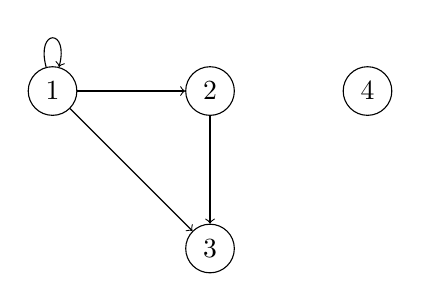
\begin{tikzpicture}[->,node distance=2cm]
  \node[draw,circle] (A) {$1$};
  \node[draw,circle] (B) [right of=A] {$2$};
  \node[draw,circle] (C) [below of=B] {$3$};
  \node[draw,circle] (D) [right of=B] {$4$};
  \draw (A) to [loop above]  (A);
  \draw (A) to  (B);
  \draw (A) to  (C);
  \draw (B) to  (C);
  \end{tikzpicture}
\intertext{Iki beda karo graf $\tuple{V', E}$ kanthi $V' =
  \{1, 2, 3\}$, kang katon kaya mangkene:}
& 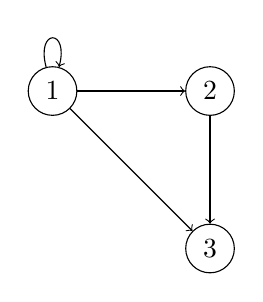
\begin{tikzpicture}[->,node distance=2cm]
  \node[draw,circle] (A) {$1$};
  \node[draw,circle] (B) [right of=A] {$2$};
  \node[draw,circle] (C) [below of=B] {$3$};
  \draw (A) to [loop above]  (A);
  \draw (A) to  (B);
  \draw (A) to  (C);
  \draw (B) to  (C);
  \end{tikzpicture}
\end{align*}
\end{ex}

\begin{prob}
  Anggepen relasi kurang saka utawa padha karo~$\le$
  ing himpunan $\{1,2, 3, 4\}$ minangka graf,
  banjur gambarna diagram kang cocog.
\end{prob}

\end{document}
\end{filecontents*}

% content/sets-functions-relations/relations/operations.tex
\begin{filecontents*}[overwrite]{slc-module-130.tex}
% Part: sets-functions-relations
% Chapter: relations
% Section: operations

\documentclass[../../../include/open-logic-section]{subfiles}

\begin{document}

\olfileid[jv]{sfr}{rel}{ops}
\olsection{Operasi tumrap Relasi}

Asring migunani yen ngowahi utawa nggabungake relasi.
Ing \olref[sfr][rel][ord]{prop:stricttopartial},
kita ngrembug \emph{gabungan} relasi, kang mung
gabungan rong relasi nalika dianggep himpunan pasangan.
Semono uga, ing \olref[sfr][rel][ord]{prop:partialtostrict},
kita ngrembug selisih relatif relasi.
Ing ngisor iki ana sawetara operasi liyane
kang bisa ditindakake tumrap relasi.

\begin{defn}\ollabel{relationoperations}
Umpamakna $R$ lan $S$ iku relasi, lan $A$ iku himpunan apa wae.

\emph{Invers} saka $R$ yaiku
$R^{-1} = \Setabs{\tuple{y, x}}{\tuple{x,y} \in R}$.

\emph{Produk relatif} saka $R$ lan $S$ yaiku
$(R \mid S) =\{\tuple{x, z} : \exists y(Rxy \land Syz)\}$.
Ing prodhuk iki, tindakna relasi kapisan dhisik, banjur relasi kapindho.

\emph{Watesan} saka $R$ ing $A$ yaiku
$\funrestrictionto{R}{A}= R\cap A^2$.

\emph{Aplikasi} saka $R$ marang $A$ yaiku
$\funimage{R}{A} = \{y :( \exists x \in A)Rxy\}$
\end{defn}

\begin{ex}
Umpamakna $S \subseteq \Int^2$ iku relasi panerus
ing~$\Int$, yaiku
$S = \Setabs{\tuple{x, y} \in \Int^2}{x + 1 = y}$,
mula $Sxy$ yen lan mung yen $x + 1 = y$.

$S^{-1}$ iku relasi pandhisik ing $\Int$, yaiku
$\Setabs{\tuple{x,y}\in\Int^2}{x -1 =y}$.

$S\mid S$ yaiku
$ \Setabs{\tuple{x,y}\in\Int^2}{x + 2 =y}$

$\funrestrictionto{S}{\Nat}$ iku relasi panerus ing~$\Nat$.

$\funimage{S}{\{1,2,3\}}$ yaiku $\{2, 3, 4\}$.
\end{ex}

\begin{defn}[Tutupan transitif]Umpamakna $R \subseteq A^2$ iku relasi biner.

\emph{Tutupan transitif} saka~$R$ yaiku
$R^+ = \bigcup_{0 < n \in\Nat} R^n$,
kanthi definisi rekursif $R^1 = R$ lan
$R^{n+1} = R^n\mid R$.
Ing perangan iki, tandha plus mratélakaké tutupan transitif.

\emph{Tutupan refleksif transitif} saka $R$ yaiku
$R^* = R^+ \cup\Id{A}$.
\end{defn}

\begin{ex}
Jupuk relasi panerus $S \subseteq \Int^2$.
$S^2xy$ yen lan mung yen $x + 2 =y$,
$S^3xy$ yen lan mung yen $x + 3 = y$,
lan sapanunggalane.
Mula $S^+xy$ yen lan mung yen $x + n = y$
kanggo sawijining $n \geq 1$.
Kanthi tembung liya, $S^+xy$ yen lan mung yen
$x < y$, lan $S^*xy$ yen lan mung yen $x \le y$.
\end{ex}

\begin{prob}
Tuduhna yen tutupan transitif saka $R$ pancen transitif.
\end{prob}

\end{document}
\end{filecontents*}

% content/sets-functions-relations/relations/orders.tex
\begin{filecontents*}[overwrite]{slc-module-131.tex}
% Part: sets-functions-relations
% Chapter: relations
% Section: orders

\documentclass[../../../include/open-logic-section]{subfiles}

\begin{document}

\olfileid[jv]{sfr}{rel}{ord}
\olsection{Tatanan}

\begin{explain}
Akeh pambandhing kita nggambarake objek minangka
"kurang saka", "padha karo", utawa "luwih saka" objek
liyane ing sawijining babagan. Iki nggunakake relasi
\emph{tatanan}. Nanging ana maneka jinis relasi tatanan.
Tuladhane, sawetara mbutuhake saben rong objek bisa
dibandhingake, dene liyane ora.
Sawetara nyakup identitas (kaya~$\le$), lan sawetara
ora nyakup (kaya~$<$).
Panggolongan bakal migunani ing kene.
\end{explain}

\begin{defn}[Pratatanan]
Relasi kang refleksif lan transitif diarani \emph{pratatanan}.
\end{defn}

\begin{defn}[Tatanan parsial]
Pratatanan kang uga antisimetris diarani \emph{tatanan parsial}.
\end{defn}

\begin{defn}[Tatanan linear]\ollabel{def:linearorder}
Tatanan parsial kang uga koneks diarani
\emph{tatanan total} utawa \emph{tatanan linear}.
\end{defn}

\begin{ex}
Saben tatanan linear uga tatanan parsial, lan saben
tatanan parsial uga pratatanan, nanging kosok baline
ora lumaku. Relasi universal ing~$A$ iku pratatanan,
amarga refleksif lan transitif. Nanging yen $A$ duwe
luwih saka siji !!{element}, relasi universal ora
antisimetris, mula dudu tatanan parsial.
\end{ex}

\begin{ex}
Gatekna relasi \emph{ora luwih dawa tinimbang}
$\preccurlyeq$ ing~$\Bin^*$:
$x \preccurlyeq y$ yen lan mung yen
$\len{x} \le \len{y}$.
Iki pratatanan (refleksif lan transitif), malah uga
koneks, nanging dudu tatanan parsial amarga ora
antisimetris. Tuladhane, $01\preccurlyeq 10$ lan
$10 \preccurlyeq 01$, nanging $01 \neq 10$.
\end{ex}

\begin{ex}
Tatanan parsial kang wigati yaiku relasi $\subseteq$
ing himpunan kang ngemot himpunan-himpunan.
Umume iki dudu tatanan linear, amarga yen $a \neq b$
lan kita ngrembug
$\Pow{\{a, b\}} = \{\emptyset, \{a\}, \{b\}, \{a,b\}\}$,
kita weruh yen $\{a\} \nsubseteq \{b\}$,
$\{a\} \neq \{b\}$, lan $\{b\}\nsubseteq \{a\}$.
\end{ex}

\begin{ex}
Relasi \emph{paran tanpa turah} menehi tatanan
parsial kang dudu tatanan linear.
Kanggo wilangan wutuh $n$ lan~$m$,
kita nulis $n \mid m$ kanggo nyatakake yen $n$
mbagi $m$ tanpa turah, yaiku yen lan mung yen
ana wilangan wutuh~$k$ kanthi $m = kn$.
Definisi iki uga maringi $0\mid 0$. Yèn wilangan kapisan nol,
mung nol kang cocog karo persamaan ing definisi.
Ing~$\Nat$, iki tatanan parsial nanging dudu
tatanan linear: tuladhane, $2 \nmid 3$ lan uga
$3 \nmid 2$. Yen dianggep relasi ing $\Int$,
relasi paran tanpa turah iki mung pratatanan amarga ora
antisimetris: $1 \mid -1$ lan $-1 \mid 1$,
nanging $1 \neq -1$.
\end{ex}

\begin{ex}
Relasi \emph{ekstensi} ing himpunan urutan~$A^*$
yaiku mangkene: $s \sqsubseteq s'$ yen lan mung yen
$s = \emptyseq$ (urutan kosong), $s = s'$,
utawa $s = \tuple{s_1, \dots, s_n}$ lan
$s' =\tuple{s_1, \dots, s_n, s_{n+1}, \dots, s_m}$.
Yen $s \sqsubseteq s'$, kita uga nyebut $s$
minangka \emph{perangan wiwitan} saka~$s'$.
Relasi ekstensi ing $A^*$ iku tatanan parsial.
Yèn alfabeté ngemot paling ora rong lambang, tatanan iki
ora linear, amarga yèn
$a \neq b$, mula $ab \not\sqsubseteq ba$ lan
$ba \not\sqsubseteq ab$. Yèn alfabeté kosong, mung ana tembung kosong.
Yèn mung ana siji lambang, saben loro tembung bisa dibandhingaké
manut dawané.
\end{ex}

\begin{defn}[Tatanan ketat]
\emph{Tatanan ketat} yaiku relasi kang irrefleksif,
asimetris, lan transitif.
\end{defn}

\begin{defn}[Tatanan linear ketat]\ollabel{def:strictlinearorder}
Tatanan ketat kang uga koneks diarani
\emph{tatanan total ketat} utawa \emph{tatanan linear ketat}.
\end{defn}

\begin{ex}
$\le$ iku tatanan linear kang cocog karo
tatanan linear ketat~$<$.
$\subseteq$ iku tatanan parsial kang cocog karo
tatanan ketat~$\subsetneq$.
\end{ex}

Saben tatanan ketat $R$ ing~$A$ bisa diowahi dadi
tatanan parsial kanthi nambah diagonal $\Id{A}$,
yaiku nambah kabeh pasangan~$\tuple{x,x}$.
(Iki diarani \emph{tutupan refleksif} saka~$R$.)
Kosok baline, saka tatanan parsial kita bisa oleh
tatanan ketat kanthi mbuwang~$\Id{A}$.
Rong asil sabanjure njlentrehake iki kanthi persis.

\begin{prop}\ollabel{prop:stricttopartial}
Yen $R$ iku tatanan ketat ing~$A$,
mula $R^+ = R \cup \Id{A}$ iku tatanan parsial.
Kajaba iku, yen $R$ iku tatanan linear ketat,
mula $R^+$ iku tatanan linear.
\end{prop}

\begin{proof}
Umpamakna $R$ iku tatanan ketat, yaiku
$R \subseteq A^2$ lan $R$ irrefleksif,
asimetris, lan transitif.
Tetepna $R^+ = R \cup \Id{A}$.
Kita kudu nuduhake yen $R^+$ refleksif,
antisimetris, lan transitif.

$R^+$ cetha refleksif, amarga
$\tuple{x, x} \in \Id{A} \subseteq R^+$
kanggo kabeh $x \in A$.

Kanggo nuduhake yen $R^+$ antisimetris,
umpamakna kanggo bukti kanthi kontradiksi yen
$R^+xy$ lan $R^+yx$ nanging $x \neq y$.
Amarga $\tuple{x,y} \in R \cup \Id{A}$,
nanging $\tuple{x, y} \notin \Id{A}$,
kita kudu duwe $\tuple{x, y} \in R$, yaiku $Rxy$.
Semono uga,~$Ryx$.
Nanging iki nalisir anggepan yen $R$ asimetris.

Kanggo mbuktekake transitivitas, umpamakna
$R^+xy$ lan $R^+yz$.
Yen $\tuple{x, y} \in R$ lan $\tuple{y,z} \in R$
loro-lorone lumaku, mula $\tuple{x, z} \in R$
amarga $R$~transitif.
Yen ora, mula $\tuple{x, y} \in\Id{A}$,
yaiku $x = y$, utawa $\tuple{y, z} \in \Id{A}$,
yaiku $y = z$.
Ing kasus kapisan, kita duwe $R^+yz$ miturut
anggepan lan $x = y$, mula $R^+xz$.
Semono uga ing kasus kapindho.
Ing saben kasus, $R^+xz$, mula $R^+$
uga transitif.

Tumrap pratelan "kajaba iku", umpamakna $R$
uga koneks. Mula kanggo kabeh $x \neq y$,
$Rxy$ utawa~$Ryx$, yaiku
$\tuple{x, y} \in R$ utawa $\tuple{y, x} \in R$.
Amarga $R \subseteq R^+$, iki tetep lumaku
tumrap $R^+$, mula $R^+$ uga koneks.
\end{proof}

\begin{prop}\ollabel{prop:partialtostrict}
Yen $R$ iku tatanan parsial ing~$A$,
mula $R^- = R \setminus \Id{A}$ iku tatanan ketat.
Kajaba iku, yen $R$ iku tatanan linear,
mula $R^-$ iku tatanan linear ketat.
\end{prop}

\begin{proof}
Iki ditinggalake minangka latihan.
\end{proof}

\begin{prob}
Wenehana bukti kanggo \olref[sfr][rel][ord]{prop:partialtostrict}.
\end{prob}

Asil prasaja ing ngisor iki nuduhake yen
tatanan linear ketat nduweni sipat kang
padha karo ekstensionalitas:

\begin{prop}\ollabel{prop:extensionality-strictlinearorders}
Yen $<$ iku tatanan linear ketat ing $A$, mula:
\[
  (\forall a, b \in A)((\forall x \in A)(x < a \liff x < b) \lif a = b).
\]
\end{prop}

\begin{proof}
Umpamakna $(\forall x \in A)(x < a \liff x < b)$.
Yen $a < b$, mula $a <a$,
kang nalisir kasunyatan yen $<$ irrefleksif;
mula $a \nless b$.
Kanthi cara kang persis padha, $b \nless a$.
Mula $a = b$, amarga $<$ koneks.
\end{proof}

\end{document}
\end{filecontents*}

% content/sets-functions-relations/relations/relations-as-sets.tex
\begin{filecontents*}[overwrite]{slc-module-132.tex}
% Part: sets-functions-relations
% Chapter: relations
% Section: relations-as-sets

\documentclass[../../../include/open-logic-section]{subfiles}

\begin{document}

\olfileid[jv]{sfr}{rel}{set}
\olsection{Relasi minangka Himpunan}

\begin{explain}
Ing \olref[sfr][set][imp]{sec}, kita nyebut sawetara himpunan
wigati: $\Nat$, $\Int$, $\Rat$, $\Real$. Mesthine kita eling
sawetara relasi kang narik kawigaten ing antarane !!{element}s
saka sawetara himpunan iki. Tuladhane, saben himpunan kasebut
duwe \emph{relasi tatanan} kang wis lumrah banget.
Uga ana relasi \emph{padha karo}, kang dumadi antarane saben objek
lan awake dhewe, nanging ora antarane objek kasebut lan objek liyane.
Ana luwih akeh relasi kang narik kawigaten kang bakal kita temoni,
lan luwih akeh maneh relasi kang bisa ana. Nanging sadurunge
ngrembug iku, kita bakal miwiti kanthi nuduhake yen relasi bisa
dianggep minangka jinis himpunan khusus.

Kanggo iki, elinga rong bab saka \olref[sfr][set][pai]{sec}.
Kapisan, elinga gagasan \emph{pasangan urut}: kanthi ana $a$ lan $b$,
kita bisa mbentuk~$\tuple{a, b}$. Ing kene urutan anggota
\emph{pancen} wigati. Mula yen $a \neq b$,
banjur $\tuple{a, b} \neq \tuple{b, a}$.
(Ing kasus loro unsur mau béda, pasangan tanpa urutan nduwèni
$2$ anggota, kanthi $\{a, b\}=\{b, a\}$.)
Kapindho, elinga gagasan \emph{produk Kartesius}:
yen $A$ lan $B$ iku himpunan, kita bisa mbentuk~$A \times B$,
himpunan kabeh pasangan $\tuple{x, y}$ kanthi $x \in A$
lan $y \in B$. Mligine, $A^{2}= A \times A$ iku
himpunan kabeh pasangan urut saka~$A$.

Saiki kita ngrembug relasi tartamtu ing sawijining himpunan:
relasi-$<$ ing himpunan~$\Nat$ saka wilangan asli.
Gatekna himpunan kabeh pasangan wilangan $\tuple{n, m}$
kanthi $n<m$, yaiku,
\[
  R=\Setabs{\tuple{n, m}}{n, m \in \Nat \text{ lan } n<m}.
\]
Ana gayutan kang raket antarane $n$ kurang saka $m$ lan
pasangan $\tuple{n, m}$ kalebu ing $R$, yaiku:
\[
      n<m\text{ yen lan mung yen }\tuple{n, m} \in R.
\]
Tanpa kelangan informasi, kita bisa nganggep himpunan $R$
\emph{minangka} relasi-$<$ ing $\Nat$.

Kanthi cara kang padha, kita bisa mbentuk subhimpunan saka
$\Nat^{2}$ kanggo saben relasi antarane wilangan.
Kosok baline, kanggo saben himpunan pasangan wilangan
$S \subseteq \Nat^{2}$, ana relasi wilangan kang cocog:
yaiku relasi antarane $n$ lan $m$ kang lumaku yen lan mung yen
$\tuple{n, m} \in S$. Iki mbenerake definisi ing ngisor iki:
\end{explain}

\begin{defn}[Relasi biner]
\emph{Relasi biner} ing himpunan $A$ yaiku subhimpunan
saka~$A^{2}$. Yen $R\subseteq A^{2}$ iku relasi biner
ing~$A$ lan $x, y \in A$, kadhangkala kita nulis
$Rxy$ (utawa $xRy$) kanggo $\tuple{x, y} \in R$.
\end{defn}

\begin{ex}
  \ollabel{relations}
Himpunan $\Nat^{2}$ saka pasangan wilangan asli bisa
ditata ing matriks rong dimensi kaya mangkene:
\[
  \begin{array}{ccccc}
  \mathbf{\tuple{ 0,0 }} & \tuple{ 0,1 } &
    \tuple{ 0,2 } & \tuple{ 0,3 } & \ldots\\
  \tuple{ 1,0 } & \mathbf{\tuple{ 1,1 }} &
    \tuple{ 1,2 } & \tuple{ 1,3 } & \ldots\\
  \tuple{ 2,0 } & \tuple{ 2,1 } &
    \mathbf{\tuple{ 2,2 }} & \tuple{ 2,3 } & \ldots\\
  \tuple{ 3,0 } & \tuple{ 3,1 } & \tuple{ 3,2 } &
    \mathbf{\tuple{ 3,3 }} & \ldots\\
  \vdots & \vdots & \vdots & \vdots & \mathbf{\ddots}
  \end{array}
\]
Diagonal ing kene dicithak kandel, amarga subhimpunan saka
$\Nat^2$ kang ngemot pasangan ing diagonal, yaiku,
\[
  \{\tuple{0,0 }, \tuple{ 1,1 }, \tuple{ 2,2 }, \dots\},
  \]
iku \emph{relasi identitas ing}~$\Nat$.
(Amarga relasi identitas kerep digunakake, kita netepake
$\Id{A}=\Setabs{\tuple{ x,x }}{x \in A}$ kanggo saben himpunan $A$.)
Subhimpunan kabeh pasangan kang ana ing sadhuwure diagonal, yaiku,
\[
  L = \{\tuple{ 0,1 },\tuple{ 0,2 },\ldots,\tuple{ 1,2 },
  \tuple{ 1,3 }, \dots, \tuple{ 2,3 }, \tuple{ 2,4 },\ldots\},
\]
iku relasi \emph{kurang saka}, yaiku $Lnm$ yen lan mung yen $n<m$.
Subhimpunan pasangan kang ana ing sangisore diagonal, yaiku,
\[
  G=\{ \tuple{ 1,0 },\tuple{ 2,0 },\tuple{
    2,1 }, \tuple{ 3,0 },\tuple{ 3,1 },\tuple{ 3,2 }, \dots\},
\]
iku relasi \emph{luwih saka}, yaiku $Gnm$ yen lan mung yen $n>m$.
Gabungan $L$ karo $I=\Id{\Nat}$, kang bisa kita jenengi $K=L\cup I$,
iku relasi \emph{kurang saka utawa padha karo}:
$Knm$ yen lan mung yen $n \le m$.
Semono uga, $H=G \cup I$ iku \emph{relasi luwih saka
utawa padha karo}. Relasi $L$, $G$, $K$, lan $H$ iki
jinis relasi khusus kang diarani \emph{tatanan}.
$L$ lan $G$ duwe sipat yen ora ana wilangan kang sesambungan
karo awake dhewe miturut relasi $L$ utawa $G$
(yaiku, kanggo kabeh $n$, ora $Lnn$ lan ora $Gnn$).
Relasi kang duwe sipat iki diarani \emph{irrefleksif};
yen relasi kasebut uga tatanan, diarani \emph{tatanan ketat}.
\end{ex}

\begin{explain}
Sanajan tatanan lan identitas iku relasi kang wigati lan lumrah,
kudu ditegesake yen miturut definisi kita, \emph{saben}
subhimpunan saka $A^{2}$ iku relasi ing~$A$,
ora preduli sepira ora lumrah utawa katon digawe-gawe.
Mligine, $\emptyset$ iku relasi ing saben himpunan
(\emph{relasi kosong}, kang ora ngemot pasangan anggota apa wae),
lan $A^{2}$~dhewe uga relasi ing~$A$
(kang ngemot saben pasangan), diarani \emph{relasi universal}.
Nanging bab kaya
$E=\Setabs{\tuple{n, m}}{n,m\in\Nat \text{ lan }(n>5 \text{ utawa } m \times n \ge 34)}$
uga dianggep relasi.
\end{explain}

\begin{prob}
  Dhaptarna !!{element}s relasi $\subseteq$ ing himpunan
  $\Pow{\{a, b, c\}}$.
\end{prob}

\end{document}
\end{filecontents*}

% content/sets-functions-relations/relations/relations.tex
\begin{filecontents*}[overwrite]{slc-module-133.tex}
% Part: sets-functions-relations
% Chapter: relations

\documentclass[../../../include/open-logic-chapter]{subfiles}

\begin{document}

\olchapter{sfr}{rel}{Relasi}

\slcEmbeddedImport{slc-module-132.tex}

\slcEmbeddedImport{slc-module-134.tex}

\slcEmbeddedImport{slc-module-128.tex}

\slcEmbeddedImport{slc-module-131.tex}

\slcEmbeddedImport{slc-module-129.tex}

\slcEmbeddedImport{slc-module-135.tex}

\slcEmbeddedImport{slc-module-130.tex}

\OLEndChapterHook

\end{document}
\end{filecontents*}

% content/sets-functions-relations/relations/special-properties.tex
\begin{filecontents*}[overwrite]{slc-module-134.tex}
% Part: sets-functions-relations
% Chapter: relations
% Section: special-properties

\documentclass[../../../include/open-logic-section]{subfiles}

\begin{document}

\olfileid[jv]{sfr}{rel}{prp}
\olsection{Sipat Khusus Relasi}

\begin{intro}
Sawetara jinis relasi kerep banget ditemoni nganti diwenehi
jeneng khusus. Tuladhane, $\le$ lan~$\subseteq$
nggayutake anggotane ranah dhewe-dhewe
(umpamane, $\Nat$ kanggo~$\le$ lan
$\Pow{A}$ kanggo~$\subseteq$) kanthi cara kang padha.
Kanggo mangerteni kanthi persis kepriye relasi kasebut
padha lan bedane, kita nggolongake relasi
miturut sawetara sipat khusus kang bisa diduweni.
Pranyata sawetara sipat khusus iki (utawa gabungane)
wigati banget: tatanan lan relasi ekuivalensi.
\end{intro}

\begin{defn}[Refleksivitas]
Relasi $R \subseteq A^2$ iku \emph{refleksif} yen lan mung yen,
kanggo saben $x \in A$, $Rxx$.
\end{defn}

\begin{defn}[Transitivitas]
Relasi $R \subseteq A^2$ iku \emph{transitif} yen lan mung yen,
manawa $Rxy$ lan $Ryz$ lumaku, $Rxz$ uga lumaku.
\end{defn}

\begin{defn}[Simetri]
Relasi~$R \subseteq A^2$ iku \emph{simetris} yen lan mung yen,
manawa $Rxy$ lumaku, $Ryx$ uga lumaku.
\end{defn}

\begin{defn}[Antisimetri]
Relasi~$R \subseteq A^2$ iku \emph{antisimetris} yen lan mung yen,
manawa $Rxy$ lan $Ryx$ lumaku bebarengan, mula $x=y$
(utawa, kanthi tembung liya: yen $x\neq y$,
mula $\lnot Rxy$ utawa $\lnot Ryx$).
\end{defn}

\begin{explain}
Ing relasi simetris, $Rxy$ lan $Ryx$ tansah lumaku
bebarengan, utawa loro-lorone ora lumaku.
Ing relasi antisimetris, siji-sijine cara supaya $Rxy$
lan $Ryx$ lumaku bebarengan yaiku yen $x = y$.
Gatekna yen syarat iki ora \emph{mbutuhake} $Rxy$ lan $Ryx$
lumaku nalika $x = y$; syarat iki mung ora nglarang bab kasebut.
Mula relasi antisimetris bisa refleksif, nanging ora
saben relasi antisimetris iku refleksif.
Uga gatekna yen antisimetris lan mung ora simetris iku
syarat kang beda. Nyatane, relasi bisa simetris lan
antisimetris bebarengan (tuladhane, relasi identitas).
\end{explain}

\begin{defn}[Koneksitas]
Relasi $R \subseteq A^2$ iku \emph{koneks} yen kanggo kabeh
$x,y\in A$, yen $x \neq y$, mula $Rxy$ utawa~$Ryx$.
\end{defn}

\begin{prob}
Wenehana tuladha relasi kang (a) refleksif lan simetris
nanging ora transitif, (b) refleksif lan antisimetris,
(c) antisimetris, transitif, nanging ora refleksif, lan
(d) refleksif, simetris, lan transitif.
Gunakna objek saben dina kanggo ranah tuladha iki.
\end{prob}

\begin{defn}[Irrefleksivitas]
Relasi $R \subseteq A^2$ diarani \emph{irrefleksif}
yen, kanggo kabeh $x \in A$, $Rxx$ ora lumaku.
\end{defn}

\begin{defn}[Asimetri]
Relasi $R \subseteq A^2$ diarani \emph{asimetris}
yen, kanggo saben pasangan $x,y\in A$, $Rxy$ lan~$Ryx$
ora tau lumaku bebarengan.
\end{defn}

Gatekna yen $A \neq \emptyset$, mula ora ana relasi
irrefleksif ing~$A$ kang refleksif. Ing ranah kosong,
relasi kosong nyukupi loro sipat mau. Saben relasi
asimetris ing~$A$ uga antisimetris ing sembarang ranah.
Yèn ranahé paling ora rong anggota, ana $R \subseteq A^2$ kang
ora refleksif lan uga ora irrefleksif. Umpamané, wènèhana gelung marang
siji anggota waé. Ing ranah sing ora kosong, relasi
identitas antisimetris lan nduwèni gelung.

\end{document}
\end{filecontents*}

% content/sets-functions-relations/relations/trees.tex
\begin{filecontents*}[overwrite]{slc-module-135.tex}
% Part: sets-functions-relations
% Chapter: relations
% Section: trees

\documentclass[../../../include/open-logic-section]{subfiles}

\begin{document}

\olfileid[jv]{sfr}{rel}{tre}
\olsection{Wit}

Jinis tatanan parsial tartamtu kang nduweni peran wigati
ing kabeh perangan logika yaiku \emph{wit}.
Wit winates katon ing perangan dhasar logika:
tuladhane, !!{formula}s bisa dingerteni lumantar
panguraiane dadi wit sintaksis, dene !!{derivation}s
ing akeh sistem !!{derivation} uga awujud wit winates.
%
Wit tanpa wates wis katon ing bukti teorema-teorema
kelengkapan kanggo logika proposisional lan logika
tataran kapisan, lan digunakake ing saindenging logika matematis.

Konsep wit ing teori himpunan raket gayutane karo
gagasan wit ing teori graf.
Iki gambar sawijining wit (winates):

\begin{center}
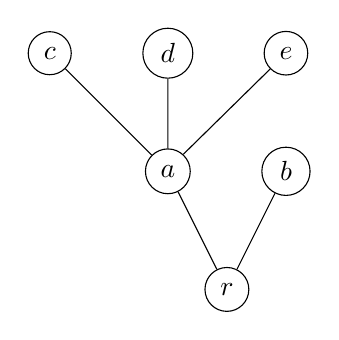
\begin{tikzpicture}[nodes={draw, circle}, -]
\node{$r$} [grow'=up]
    child { node {$a$}
        child { node {$c$} }
        child { node {$d$} }
        child { node {$e$} }
    }
    child { node {$b$} };
\end{tikzpicture}
\end{center}

Simpul paling ngisor~$r$ iku oyod.
Saben simpul saliyane $r$ duwe persis siji simpul induk
langsung ing sangisore. Kita bisa nganggep relasi
antarane simpul~$x$ lan simpul~$y$---yen
$y$ bisa digayuh saka~$x$ kanthi ngetutaké siji utawa luwih rusuk
munggah---minangka pratelan yen $x$ iku \emph{leluhur} saka~$y$.

Relasi leluhur ing wit iku tatanan parsial ketat.
Iki dadi dhasar definisi miturut teori himpunan.
Kanggo nyatakake, kita mbutuhake rong konsep.
\emph{Anggota paling cilik} ing himpunan~$A$
kang ditata parsial dening~$\le$ yaiku
!!a{element} $x \in A$ kanthi sipat yen
kanggo kabeh $y \in A$ kita duwe~$x \le y$.
Himpunan \emph{katata kanthi becik} dening~$\le$
yen saben subhimpunane kang ora kosong duwe
anggota paling cilik.

\begin{defn}[Wit]
\emph{Wit} yaiku pasangan $T = \tuple{A, \le}$
kanthi syarat yen $A$ iku himpunan lan $\le$
iku tatanan parsial ing~$A$ kanthi siji-sijine
anggota paling cilik $r \in A$
(diarani \emph{oyod}), lan kanggo kabeh $x \in A$,
himpunan $\Setabs{y}{y \le x}$
katata kanthi becik dening~$\le$.
\end{defn}

\begin{defn}[Panerus]
Umpamakna $T = \tuple{A, \le}$ iku wit.
Yen $x,y \in A$, $x < y$, lan ora ana
$z \in A$ kanthi $x < z < y$,
mula kita nyebut $y$ minangka \emph{panerus} saka~$x$.
\end{defn}

Panerus-panerus saka $x \in A$ uga diarani \emph{anake}.
Yen $y$ iku panerus saka~$x$, mula kita nyebut $x$
minangka \emph{pandhisik} utawa \emph{induk} saka~$y$.

\begin{prop}
Yen $\tuple{A,\le}$ iku wit, mula saben $x \in A$
saliyane oyod duwe paling akeh siji pandhisik.
\end{prop}

\begin{proof}
  Umpamakna $y_1 < x$, $y_2 < x$, lan $y_1 \neq y_2$.
  Mula $\{y_1,y_2\} \subseteq \Setabs{z}{z<x}$.
  Amarga $\Setabs{z}{z<x}$ katata kanthi becik
  dening~$\le$, subhimpunane $\{y_1, y_2\}$
  duwe anggota paling cilik, kang mesthi
  $y_1$ utawa~$y_2$.
  Mula $y_1 \le y_2$ utawa $y_2 \le y_1$.
  Kita nganggep $y_1 \neq y_2$, mula sejatine
  $y_1 < y_2$ utawa $y_2 < y_1$.
  Amarga kita nganggep $y_1 < x$ lan $y_2 < x$,
  kita uga duwe $y_1 < y_2< x$ utawa
  $y_2 < y_1 < x$.
  Mula $y_1$ lan $y_2$ ora bisa loro-lorone
  dadi pandhisik saka~$x$.
\end{proof}
Wit winates nduwèni pandhisik kanggo saben simpul saliyané oyod.
Ing wit tanpa wates, sawijining segmèn ngisor bisa tanpa
anggota paling gedhé, mula simpulé bisa tanpa pandhisik.

\begin{defn}
Wit $T = \tuple{A, \le}$ diarani \emph{tanpa wates}
yen $A$ iku himpunan tanpa wates, lan
\emph{winates} yen ora mangkono.
Yen $T$ nduweni sipat saben $x \in A$
mung duwe panerus kang cacahe winates,
mula kita nyebut $T$ \emph{nyabang winates}.
\end{defn}

\begin{defn}[Pang]
Kanggo wit $T = \tuple{A, \le}$, \emph{pang} saka~$T$
yaiku rantai maksimal ing~$T$, yaiku himpunan
$B \subseteq A$ kanthi sipat yen kanggo saben
$x, y \in B$, $x \le y$ utawa $y \le x$,
lan kanggo saben $z \in A \setminus B$
ana $u \in B$ kanthi $z \le u$ lan $u \le z$
loro-lorone ora lumaku.
%
Kita nganggo $[T]$ kanggo nglambangake
himpunan kabeh pang saka $T$.
\end{defn}

\begin{ex}
Tuladha klasik wit kang nyabang winates yaiku
\emph{wit biner tanpa wates} saka urutan winates
kang unsur-unsure $0$ utawa~$1$, kadhangkala
dilambangake $\{0,1\}^*$ utawa~$\Bin^*$,
ditata nganggo relasi ekstensi $\sqsubseteq$
(tuladhane, $101 \sqsubseteq 101101$).
Amarga saben rerangken biner tansah bisa
ditambahi $0$ utawa $1$ ing pungkasane,
wit iki ngemot anggota kang cacahe tanpa wates:
saben anggota~$s$ duwe persis rong panerus,
$s0$ lan~$s1$.
Oyode yaiku urutan kosong $\emptyseq$.
\end{ex}

\begin{ex}
Kanthi rada luwih umum, himpunan urutan winates
wilangan asli~$\Nat^*$ kanthi relasi
ekstensi~$\sqsubseteq$ uga wit.
Cetha yen wit iki ora nyabang winates:
saben $s \in \Nat^*$ duwe panerus~$sn$
kang cacahe tanpa wates, siji kanggo saben
$n \in \Nat$.
Saben $A\subseteq \Nat^*$ kang ora kosong lan katutup
tumrap~$\sqsubseteq$ iku \emph{subwit}
saka~$\Nat^*$.
(Yaiku, $A$ nduweni sipat yen $s \in A$
lan $s' \sqsubseteq s$, mula uga $s' \in A$.)
Kabèh wit winates bisa diwakili minangka subwit winates saka~$\Nat^*$.
Wènèhana nomer béda marang anak saka saben simpul, banjur catheten
urutan nomer ing dalan saka oyod menyang simpul kasebut.
\end{ex}

\begin{prop}[Lema K\H{o}nig]
Yen $T = \tuple{A,\le}$ iku wit tanpa wates
kang nyabang winates, mula $T$
duwe pang tanpa wates.
\end{prop}

Kasus khusus lema K\H{o}nig kang akeh digunakake
ing teori komputabilitas, dikenal minangka
\emph{lema K\H{o}nig ringkih}, yaiku mangkene:
saben subwit tanpa wates saka $\{0,1\}^*$
duwe pang tanpa wates.

\end{document}
\end{filecontents*}

% content/sets-functions-relations/sets-functions-relations.tex
\begin{filecontents*}[overwrite]{slc-module-136.tex}
% Part: Sets, Relations, Functions

\documentclass[../../include/open-logic-part]{subfiles}

\begin{document}

\olpart{sfr}{Himpunan, Relasi, Fungsi}

\begin{editorial}
Pambuka iki ngenalaké himpunan, fungsi, relasi, lan urutan. Bagean-bagean iki menehi landhesan notasi kanggo definisi lan bukti ing logika.
\end{editorial}

\slcEmbeddedImport{slc-module-141.tex}

\slcEmbeddedImport{slc-module-133.tex}

\slcEmbeddedImport{slc-module-125.tex}

\slcEmbeddedImport{slc-module-153.tex}

\OLEndPartHook
\end{document}
\end{filecontents*}

% content/sets-functions-relations/sets/basics.tex
\begin{filecontents*}[overwrite]{slc-module-137.tex}
% Part: sets-functions-relations
% Chapter: sets
% Section: basics

\documentclass[../../../include/open-logic-section]{subfiles}

\begin{document}

\olfileid[jv]{sfr}{set}{bas}
\olsection{Ekstensionalitas}

\emph{Himpunan} yaiku kumpulan objek kang dianggep {minangka} siji
objek. Objek-objek kang mbentuk himpunan kasebut diarani \emph{unsur}
utawa \emph{anggota} himpunan. Yen $x$ iku !!a{element} himpunan~$A$,
kita nulis $x \in A$; yen ora, kita nulis $x \notin A$.
Himpunan kang ora duwe !!{element}s diarani himpunan \emph{kosong}
lan dilambangake nganggo~"$\emptyset$".

\begin{explain}
Ora dadi prakara kepriye kita \emph{nemtokake} himpunan kasebut,
kepriye kita \emph{ngurutake} !!{element}sne, utawa malah \emph{kaping
pira} kita ngetung !!{element}sne. Kang wigati mung apa wae
!!{element}sne. Bab iki kita rumusake ing prinsip ing ngisor iki.
\end{explain}

\begin{defn}[Ekstensionalitas]
  Yen $A$ lan $B$ iku himpunan, mula $A = B$ yen lan mung yen
  saben !!{element} saka~$A$ uga !!a{element} saka~$B$, lan
  kosok baline.
\end{defn}

Ekstensionalitas mbenerake panganggone sawetara notasi. Umume, yen
kita duwe objek $a_{1}$, \dots, $a_{n}$, mula $\{a_{1}, \dots, a_{n}\}$
yaiku \emph{himpunan siji-sijine} kang !!{element}sne yaiku
$a_1, \ldots, a_n$. Kita negesake tetembungan
"\emph{himpunan siji-sijine}", amarga ekstensionalitas nerangake yen
himpunan kaya mangkono mung bisa ana \emph{siji}. Ekstensionalitas uga
mbenerake pratelan iki:
  \[
    \{a, a, b\} = \{a, b\} = \{b,a\}.
  \]
Iki nuduhake yen, nalika ngrembug himpunan, kita ora nggatekake
urutane !!{element}s utawa kaping pira anggota kasebut disebutake.

\begin{tagblock}{novice}
\begin{ex}
Yen duwe sawenehing objek, objek kasebut bisa diklumpukake dadi
himpunan. Tuladhane, himpunan sedulure Richard ngemot siji wong,
lan bisa ditulis $S=\{\textrm{Ruth}\}$.
Himpunan wilangan wutuh positif kang kurang saka $4$ yaiku
$\{1, 2, 3\}$, nanging uga bisa ditulis $\{3, 2, 1\}$ utawa malah
$\{1, 2, 1, 2, 3\}$. Miturut ekstensionalitas, kabeh mau himpunan
kang padha. Amarga saben !!{element} saka $\{1, 2, 3\}$ uga
!!a{element} saka $\{3, 2, 1\}$ (lan saka $\{1,
2, 1, 2, 3\}$), lan kosok baline.
\end{ex}
\end{tagblock}

Asring kita nemtokake himpunan lumantar sawijining sipat kang
diduweni bebarengan dening !!{element}sne. Notasi iki migunakaké ranah sing wis dimangertèni. $\Setabs{x}{\phi(x)}$ iku notasi cekak, kanthi $\phi(x)$
nglambangake sipat kang kudu diduweni~$x$ supaya bisa kalebu
ing antarane !!{element}s himpunan kasebut.

\begin{tagblock}{novice}
\begin{ex}
Ing tuladha kita, $S$ uga bisa ditemtokake minangka
\[
S = \Setabs{x}{x \text{ iku sedulure Richard}}.
\]
\end{ex}
\end{tagblock}

\begin{tagblock}{math}
\begin{ex}
Wilangan wutuh positif diarani \emph{sampurna} yèn lan mung yèn padha karo
gunggungé pambagi positifé sing luwih cilik tinimbang wilangan kuwi.
Tuladhané, $6$ iku sampurna amarga pambagi positifé sing luwih cilik
yaiku $1$, $2$, lan~$3$, lan
$6 = 1 + 2 + 3$. Nyatane, $6$ iku siji-sijine wilangan wutuh
positif kang kurang saka $10$ lan sampurna. Mula, kanthi
ekstensionalitas, kita bisa nyatakake:
\[
	\{6\} = \Setabs{x}{x\text{ iku wilangan wutuh sampurna lan }0 < x < 10}
\]
Notasi ing sisih tengen diwaca "himpunan kabeh $x$ kang $x$ iku
sampurna lan $0 < x < 10$". Pepadhan iki negesake yen,
nalika ngrembug himpunan, kita ora nggatekake carane himpunan kasebut
ditemtokake. Kanthi luwih umum, ekstensionalitas njamin paling akèh ana
siji himpunan kabèh $x$ kang nduwèni sipat~$\phi(x)$.
Yèn himpunané ana, $\Setabs{x}{\phi(x)}$ iku \emph{himpunan siji-sijiné} kang
ngemot kabèh $x$ kang nduwèni sipat~$\phi(x)$.
Anané himpunan perlu dhasar, upamané milih anggota saka sawijining
himpunan kang wis ana.
\end{ex}
\end{tagblock}

Ekstensionalitas menehi cara kanggo nuduhake yen himpunan iku padha:
kanggo nuduhake $A = B$, tuduhna yen saben $x \in A$ uga $x \in B$,
lan saben $y \in B$ uga $y \in A$.

\begin{prob}
Buktekna yen himpunan kosong paling akeh ana siji, yaiku tuduhna
yen $A$ lan $B$ iku himpunan tanpa !!{element}s, mula $A = B$.
\end{prob}

\end{document}
\end{filecontents*}

% content/sets-functions-relations/sets/important-sets.tex
\begin{filecontents*}[overwrite]{slc-module-138.tex}
% Part: sets-functions-relations
% Chapter: sets
% Section: important-sets

\documentclass[../../../include/open-logic-section]{subfiles}

\begin{document}

\olfileid[jv]{sfr}{set}{imp}
\olsection{Sawetara Himpunan Wigati}

\begin{ex}
Umume kita bakal ngrembug himpunan kang !!{element}sne arupa
objek matematis. Ana papat himpunan kaya mangkono kang cukup
wigati nganti diwenehi jeneng khusus:
\begin{multline*}
    \Nat = \{0, 1, 2, 3, \ldots\} \\
    \shoveright{\text{himpunan wilangan asli}}\\
    \shoveleft{\Int = \{\ldots, -2, -1, 0, 1, 2, \ldots\}} \\
    \shoveright{\text{himpunan wilangan wutuh}}\\
    \shoveleft{\Rat = \Setabs{\nicefrac{m}{n}}{m, n \in \Int\text{ lan }n \neq 0}}\\
    \shoveright{\text{himpunan wilangan rasional}}\\
    \shoveleft{\Real = (-\infty, \infty)}\\
    \text{himpunan wilangan real (kontinuum)}
\end{multline*}
Kabèh iki himpunan \emph{tanpa wates}, yaiku saben himpunan
duwe !!{element}s kang cacahe tanpa wates.

Nalika pindhah saka himpunan siji menyang sabanjure ing dhaptar iki,
kita nambah \emph{luwih akeh} wilangan ing pasadhiyan kita.
Mesthine cetha yen $\Nat \subseteq \Int
\subseteq \Rat \subseteq \Real$: saben wilangan asli iku
wilangan wutuh; saben wilangan wutuh iku rasional; lan saben
wilangan rasional iku real. Semono uga, mesthine cetha yen
$\Nat \subsetneq \Int \subsetneq
\Rat$, amarga $-1$ iku wilangan wutuh nanging dudu wilangan asli,
lan $\nicefrac{1}{2}$ iku rasional nanging dudu wilangan wutuh.
Kang kurang cetha yaiku $\Rat \subsetneq \Real$, yaiku ana
wilangan real kang ora rasional\oliflabeldef{sfr:arith:real:realline}{,
nanging bab iki bakal dirembug maneh ing \olref[arith][real]{realline}}{}.

Kadhangkala kita uga nganggo himpunan wilangan wutuh positif
$\PosInt = \{1,2, 3, \dots\}$ lan himpunan kang mung ngemot
rong wilangan asli kapisan $\Bin = \{0, 1\}$.
\end{ex}

\begin{tagblock}{compsci}
\begin{ex}[Rerangken]
Tuladha liyane kang narik kawigaten yaiku himpunan $A^{*}$ saka
\emph{rerangken winates} ing alfabet $A$: saben urutan winates
anggota~$A$ iku rerangken ing $A$. Kita nglebokake
\emph{rerangken kosong $\Lambda$} ing antarane rerangken ing~$A$,
kanggo saben alfabet~$A$. Tuladhane,
\begin{multline*}
\Bin^*
=\{\Lambda,0,1,00,01,10,11,\\
000,001,010,011,100,101,110,111,0000,\ldots\}.
\end{multline*}
Yen $x=x_{1}\ldots x_{n}\in A^{*}$ iku rerangken kang dumadi
saka $n$ "aksara" saka $A$, mula kita nyebut \emph{dawane}
rerangkèn kasebut~$n$ lan nulis $\len{x}=n$.
\end{ex}
\end{tagblock}

\begin{ex}[Urutan tanpa wates]
Kanggo saben himpunan $A$, kita uga bisa ngrembug himpunan~$A^\omega$
saka urutan tanpa wates kang ngemot !!{element}s saka~$A$.
Urutan tanpa wates $a_1a_2a_3a_4\dots$ dumadi saka dhaptar
objek kang tanpa wates ing siji arah, lan saben objek iku
!!a{element} saka~$A$.
\end{ex}

\end{document}
\end{filecontents*}

% content/sets-functions-relations/sets/pairs-and-products.tex
\begin{filecontents*}[overwrite]{slc-module-139.tex}
% Part: sets-functions-relations
% Chapter: sets
% Section: pairs-and-products

\documentclass[../../../include/open-logic-section]{subfiles}

\begin{document}

\olfileid[jv]{sfr}{set}{pai}
\olsection{Pasangan, Tupel, Produk Kartesius}

\begin{explain}
Saka ekstensionalitas bisa didudut yen anggota himpunan ora
duwe urutan. Mula, yen arep nggambarake urutan, kita nganggo
\emph{pasangan urut} $\tuple{x, y}$. Ing pasangan tanpa urutan
$\{x, y\}$, urutan ora wigati: $\{x, y\} = \{y, x\}$.
Ing pasangan urut, urutan iku wigati: yen $x
\neq y$, mula $\tuple{x, y} \neq \tuple{y, x}$.

Kepriye kudune kita ngerteni pasangan urut ing teori himpunan?
Kang wigati, kita arep njaga gagasan yen pasangan urut iku padha
yen lan mung yen anggota kapisane padha lan anggota kapindhone
uga padha, yaiku:
\[
  \tuple{a, b}= \tuple{c, d}\text{ yen lan mung yen }a = c \text{ lan }b=d.
\]
Pasangan urut bisa ditemtokake ing teori himpunan nganggo
definisi Wiener--Kuratowski.
\end{explain}

\begin{defn}[Pasangan urut]\ollabel{wienerkuratowski}
	$\tuple{a, b} = \{\{a\}, \{a, b\}\}$.
\end{defn}

\begin{prob}
	Kanthi nggunakake \olref[sfr][set][pai]{wienerkuratowski},
	buktekna yen $\tuple{a,b}= \tuple{c, d}$ yen lan mung yen
	$a = c$ lan $b=d$.
\end{prob}

\begin{explain}
Sawise netepake definisi pasangan urut, kita bisa nggunakake
kanggo nemtokake himpunan liyane. Tuladhane, kadhangkala kita
uga mbutuhake urutan luwih saka rong objek, kayata
\emph{tupel telu} $\tuple{x, y, z}$,
\emph{tupel papat} $\tuple{x, y, z, u}$, lan sateruse.
Tupel telu bisa dianggep pasangan urut khusus kang anggota
kapisane dhewe arupa pasangan urut:
$\tuple{x, y, z}$ yaiku $\tuple{\tuple{x, y},z}$.
Semono uga kanggo tupel papat: $\tuple{x,y,z,u}$ yaiku
$\tuple{\tuple{\tuple{x,y},z},u}$, lan sateruse.
Kanthi umum, kita nyebut \emph{tupel-$n$ urut}
$\tuple{x_1, \dots, x_n}$.

Sawetara himpunan pasangan urut, utawa tupel-$n$ urut liyane,
bakal migunani.
\end{explain}

\begin{defn}[Produk Kartesius]
Kanggo himpunan $A$ lan $B$, \emph{produk Kartesius}
$A \times B$ ditemtokake kanthi
\[
  A \times B = \Setabs{\tuple{x, y}}{x \in A \text{ lan } y \in B}.
\]
\end{defn}

\begin{ex}
Yen $A = \{0, 1\}$ lan $B = \{1, a, b\}$, mula produke yaiku
\[
A \times B = \{ \tuple{0, 1}, \tuple{0, a}, \tuple{0, b},
    \tuple{1, 1}, \tuple{1, a}, \tuple{1, b} \}.
\]
\end{ex}

\begin{ex}
Yen $A$ iku himpunan, produk $A$ karo awake dhewe,
$A \times A$, uga ditulis~$A^2$. Iki himpunan
\emph{kabeh} pasangan $\tuple{x, y}$ kanthi $x, y \in A$.
Himpunan kabeh tupel telu $\tuple{x, y, z}$ yaiku $A^3$,
lan sateruse. Kita bisa menehi definisi rekursif:
\begin{align*}
  A^1 & = A\\
  A^{k+1} & = A^k \times A
\end{align*}
\end{ex}

\begin{prob}
Dhaptarna kabeh !!{element}s saka $\{1, 2, 3\}^3$.
\end{prob}

\begin{prop}\ollabel{cardnmprod}
Yen $A$ duwe $n$ !!{element}s lan $B$ duwe $m$ !!{element}s,
mula $A\times B$ duwe $n\cdot m$ anggota.
\end{prop}

\begin{proof}
Yèn salah siji faktor kosong, prodhuk uga kosong lan cacah
anggotané nol. Kanggo faktor loro sing ora kosong,
kanggo saben !!{element}~$x$ ing~$A$, ana $m$ !!{element}s
awujud $\tuple{x, y} \in A \times B$.
Tetepna $B_x = \Setabs{\tuple{x, y}}{y\in B}$.
Amarga yen $x_1 \neq x_2$,
$\tuple{x_1, y_1} \neq\tuple{x_2, y_2}$, mula
$B_{x_1} \cap B_{x_2} = \emptyset$.
Nanging yen $A = \{x_1,\dots, x_n\}$, mula
$A \times B = B_{x_1} \cup \dots \cup B_{x_n}$,
saengga duwe $n\cdot m$ !!{element}s.

Kanggo nggambarake iki, tatanen !!{element}s saka~$A \times B$
ing larik lan kolom:
\[
\begin{array}{rcccc}
  B_{x_1} = & \{\tuple{x_1, y_1} & \tuple{x_1, y_2} & \dots & \tuple{x_1, y_m}\}\\
  B_{x_2} = & \{\tuple{x_2, y_1} & \tuple{x_2, y_2} & \dots & \tuple{x_2, y_m}\}\\
  \vdots & & \vdots\\
  B_{x_n} = & \{\tuple{x_n, y_1} & \tuple{x_n, y_2} & \dots & \tuple{x_n, y_m}\}
\end{array}
\]
Amarga kabeh $x_i$ beda-beda lan kabeh $y_j$ beda-beda,
ora ana rong pasangan ing tatanan iki kang padha,
lan cacahe kabeh pasangan yaiku $n\cdot m$.
\end{proof}

\begin{prob}
Tuduhna, kanthi induksi tumrap~$k$, yen kanggo kabeh $k \ge 1$,
yen $A$ duwe $n$ !!{element}s, mula $A^k$ duwe
$n^k$ !!{element}s.
\end{prob}

\begin{ex}
Yen $A$ iku himpunan, \emph{tembung} ing~$A$ yaiku saben
urutan winates !!{element}s saka~$A$. Urutan bisa dianggep
tupel-$n$ kang ngemot !!{element}s saka~$A$.
Tuladhane, yen $A = \{a, b, c\}$, urutan "$bac$" bisa
dianggep minangka tupel telu~$\tuple{b, a, c}$.
Tembung, yaiku urutan lambang, wigati banget ing ilmu komputer.
Tembung dawané~$n$ dikodhe minangka fungsi saka
$\{1,\ldots,n\}$ menyang~$A$. Nalika $n=0$, ranahé kosong
lan fungsi kosong $\emptyset$ dadi tembung kosong. Kode
iki mbedakaké tembung kang dawané béda lumantar ranahé.
Himpunan kabèh tembung ing~$A$ yaiku
\[
A^* = \bigcup_{n\in\Nat} \Setabs{w}{w:\{1,\ldots,n\}\to A}.
\]
\end{ex}

\end{document}
\end{filecontents*}

% content/sets-functions-relations/sets/russells-paradox.tex
\begin{filecontents*}[overwrite]{slc-module-140.tex}
% Part: sets-functions-relations
% Chapter: sets
% Section: russells-paradox

\documentclass[../../../include/open-logic-section]{subfiles}


\begin{document}

\olfileid[jv]{sfr}{set}{rus}
\olsection{Paradoks Russell}

Ekstensionalitas mbenerake notasi $\Setabs{x}{\phi(x)}$ kanggo
\emph{himpunan siji-sijine} kang anggotane kabeh lan mung $x$ kang
nduweni sipat~$\phi(x)$.
Nanging, kang \emph{tenan} dibenerake dening ekstensionalitas
mung gagasan iki: \emph{yen} ana himpunan kang anggotane kabeh
lan mung objek kang nduweni sipat $\phi$, \emph{mula} himpunan
kaya mangkono mung ana siji. Kanthi tembung liya, sawisé netepaké
sawijining~$\phi$, himpunan $\Setabs{x}{\phi(x)}$ iku tunggal,
\emph{yen ana}.

Nanging pratelan mawa syarat iki wigati!{} Ora saben sipat
bisa digunakake kanggo \emph{komprehensi}. Tegese, ana sipat
kang \emph{ora} nemtokake himpunan. Yen kabeh sipat nemtokake
himpunan, kita bakal nemoni kontradiksi kang cetha.
Tuladha kang paling misuwur yaiku Paradoks Russell.

Himpunan bisa dadi !!{element}s saka himpunan liyane---tuladhane,
himpunan pangkat saka himpunan~$A$ dumadi saka himpunan-himpunan.
Mula ana tegese yen kita takon utawa nliti apa sawijining
himpunan iku !!a{element} saka himpunan liyane.
Apa himpunan bisa dadi anggota awake dhewe? Katone ora ana
apa-apa ing gagasan himpunan kang ngalangi iki.
Tuladhane, yen \emph{kabeh} himpunan mbentuk kumpulan objek,
kita bisa ngira yen kabeh mau bisa diklumpukake dadi siji
himpunan---himpunan kabeh himpunan. Lan himpunan kasebut,
amarga dhewe uga himpunan, bakal dadi !!a{element}
saka himpunan kabeh himpunan.

Paradoks Russell tuwuh nalika kita ngrembug sipat ora duwe
awake dhewe minangka !!a{element}, yaiku \emph{ora dadi anggota
awake dhewe}. Kepriye yen kita nganggep ana himpunan kabeh
himpunan kang ora duwe awake dhewe minangka !!a{element}?
Apa
\[
R = \Setabs{x}{x \notin x}
\]
ana? Pranyata kita bisa mbuktekake yen himpunan iki ora ana.

\begin{thm}[Paradoks Russell]\ollabel{thm:russells-paradox}
	Ora ana himpunan $R = \Setabs{x}{x \notin x}$.
\end{thm}

\begin{proof}
Yen $R = \Setabs{x}{x \notin x}$ ana, mula
$R \in R$ yen lan mung yen $R \notin R$, kang arupa kontradiksi.
\end{proof}

\begin{tagblock}{novice}
\begin{explain}
Ayo nlusuri bukti iki kanthi luwih alon. Yen $R$ ana,
pitakon apa $R \in R$ utawa ora iku ana tegese.
Umpamakna pancen $R \in R$. $R$~wis ditetepake minangka
himpunan kabeh himpunan kang ora dadi !!{element}s saka
awake dhewe. Mula, yen $R \in R$, $R$ dhewe ora duwe
sipat kang digunakake kanggo nemtokake $R$.
Nanging mung himpunan kang duwe sipat iki kang ana ing~$R$,
mula $R$ ora bisa dadi !!a{element} saka~$R$,
yaiku $R \notin R$. Nanging $R$ ora bisa bebarengan dadi
lan ora dadi !!a{element} saka~$R$, mula kita oleh kontradiksi.

Amarga anggepan yen $R \in R$ nuwuhake kontradiksi,
kita oleh $R \notin R$. Nanging iki uga nuwuhake kontradiksi!{}
Amarga yen $R\notin R$, $R$ dhewe pancen duwe sipat kang
digunakake kanggo nemtokake $R$, mula $R$ bakal dadi
!!a{element} saka $R$, kaya kabeh himpunan liyane kang
ora dadi anggota awake dhewe.
Lan maneh, ora bisa bebarengan ora dadi lan dadi
!!a{element} saka~$R$.
\end{explain}
\end{tagblock}

\begin{digress}
Kepriye carane mbangun teori himpunan kang ora kena Paradoks
Russell, yaiku kang ora nggawe pratelan \emph{ora konsisten}
yen $R = \Setabs{x}{x \notin x}$ ana?
Kita kudu netepake aksioma kang menehi syarat kanthi tliti banget
kanggo nyatakake kapan himpunan ana (lan kapan ora ana).

Teori himpunan kang digarisake ing bab iki ora nindakake iku.
Teori iki \emph{pancen naif}. Teori iki mung nerangake yen
himpunan manut ekstensionalitas lan yen kita duwe sawetara
himpunan, kita bisa mbentuk gabungan, irisan, lan sapanunggalane.
Teori himpunan bisa dikembangake kanthi luwih tliti tinimbang iki.
\oliflabeldef{sth:::part}{Andharan kanthi tliti kasebut diwenehake
ing Perangan \olref[sth][][]{part}. Saiki kita bakal nerusake
kanthi cara naif, lan kanthi ngati-ati ngupaya nyingkiri kontradiksi.}{}
\end{digress}


\end{document}
\end{filecontents*}

% content/sets-functions-relations/sets/sets.tex
\begin{filecontents*}[overwrite]{slc-module-141.tex}
% Part: sets-functions-relations
% Chapter: sets

\documentclass[../../../include/open-logic-chapter]{subfiles}

\begin{document}

\olchapter{sfr}{set}{Himpunan}

\slcEmbeddedImport{slc-module-137.tex}

\slcEmbeddedImport{slc-module-142.tex}

\slcEmbeddedImport{slc-module-138.tex}

\slcEmbeddedImport{slc-module-143.tex}

\slcEmbeddedImport{slc-module-139.tex}

\slcEmbeddedImport{slc-module-140.tex}

\OLEndChapterHook

\end{document}
\end{filecontents*}

% content/sets-functions-relations/sets/subsets.tex
\begin{filecontents*}[overwrite]{slc-module-142.tex}
% Part: sets-functions-relations
% Chapter: sets
% Section: subsets

\documentclass[../../../include/open-logic-section]{subfiles}

\begin{document}

\olfileid[jv]{sfr}{set}{sub}
\olsection{Subhimpunan lan Himpunan Pangkat}

\begin{explain}
Kita bakal kerep mbandhingake himpunan. Salah siji pambandhing kang
cetha yaiku: \emph{kabeh kang ana ing siji himpunan uga ana ing
himpunan liyane}. Kahanan iki cukup wigati, mula kita perlu
ngenalake notasi anyar.
\end{explain}

\begin{defn}[Subhimpunan]
Yen saben !!{element} himpunan $A$ uga !!a{element} saka~$B$,
mula kita nyebut $A$ minangka \emph{subhimpunan} saka~$B$, lan
nulis $A \subseteq B$. Yen $A$ dudu subhimpunan saka~$B$, kita
nulis $A \not\subseteq B$.
Yen $A \subseteq B$ nanging $A \neq B$, kita nulis $A \subsetneq B$
lan nyebut $A$ minangka \emph{subhimpunan sejati} saka $B$.
\end{defn}

\begin{ex}
Saben himpunan iku subhimpunan saka himpunan iku dhéwé, lan $\emptyset$
iku subhimpunan saka saben himpunan. Himpunan wilangan asli genep
iku subhimpunan saka himpunan wilangan asli.
Uga, $\{ a, b \} \subseteq \{ a, b, c \}$. Nanging
$\{ a, b, e\}$ dudu subhimpunan saka $\{ a, b, c \}$.
\end{ex}

\begin{ex}
Wilangan $2$ iku !!{element} himpunan wilangan wutuh, dene
himpunan wilangan genep iku subhimpunan saka himpunan wilangan
wutuh. Nanging, sawijining himpunan bisa \emph{bebarengan} dadi
!!a{element} lan subhimpunan saka himpunan liyane, tuladhane
$\{0\} \in \{0, \{0\}\}$ lan uga $\{0\} \subseteq \{0,
\{0\}\}$.
\end{ex}

Ekstensionalitas menehi patokan pepadhan kanggo himpunan:
$A = B$ yen lan mung yen saben !!{element} saka~$A$ uga
!!a{element} saka~$B$ lan kosok baline. Definisi "subhimpunan"
nemtokake $A \subseteq B$ persis minangka separo kapisan saka
patokan iki: saben !!{element} saka~$A$ uga !!a{element} saka~$B$.
Mesthi wae definisi iki uga lumaku yen $A$ lan $B$ diijolake:
yaiku, $B \subseteq A$ yen lan mung yen saben !!{element}
saka~$B$ uga !!a{element} saka~$A$. Iki persis perangan
"kosok baline" ing ekstensionalitas. Kanthi tembung liya,
ekstensionalitas nduweni akibat yen himpunan-himpunan iku padha
yen lan mung yen siji lan sijine padha dadi subhimpunan.

\begin{prop}
$A = B$ yen lan mung yen $A \subseteq B$ lan $B \subseteq A$.
\end{prop}

Saiki uga wektu kang trep kanggo ngenalake sawetara notasi
tambahan kang migunani. Nalika nemtokake kapan $A$ iku subhimpunan
saka~$B$, kita nyebut "saben !!{element} saka~$A$ iku \dots,"
lan ngisi "$\dots$" nganggo "!!a{element} saka $B$".
Nanging \emph{wangun} ukara iki kerep banget digunakake, mula
bakal migunani yen kita ngenalake notasi formal kanggo wangun iki.

\begin{defn}\ollabel{forallxina}
$(\forall x \in A)\phi$ minangka cekakan saka $\forall x(x \in A \lif
\phi)$. Semono uga, $(\exists x \in A)\phi$ minangka cekakan saka
$\exists x(x\in A \land \phi)$.
\end{defn}

Kanthi notasi iki, kita bisa nyatakake yen $A \subseteq B$ yen lan
mung yen $(\forall x \in A)x \in B$.

Saiki kita ngrembug jinis himpunan tartamtu: himpunan kabeh
subhimpunan saka sawijining himpunan.

\begin{defn}[Himpunan Pangkat]
Himpunan kang anggotané persis kabèh subhimpunan saka himpunan~$A$ diarani
\emph{himpunan pangkat saka}~$A$, ditulis $\Pow{A}$.
  \[
    \Pow{A} = \Setabs{B}{B \subseteq A}
  \]
\end{defn}

\begin{ex}
Apa wae kabeh subhimpunan kang bisa digawe saka $\{ a, b, c \}$?
Yaiku: $\emptyset$, $\{a \}$, $\{b\}$, $\{c\}$, $\{a, b\}$,
$\{a, c\}$, $\{b,c\}$, $\{a, b, c\}$.
Himpunan kabeh subhimpunan iki yaiku $\Pow{\{a,b,c\}}$:
\[
\Pow{\{ a, b, c \}} = \{\emptyset, \{a \}, \{b\}, \{c\}, \{a, b\},
\{b, c\}, \{a, c\}, \{a, b, c\}\}
\]
\end{ex}

\begin{prob}
Dhaptarna kabeh subhimpunan saka $\{a, b, c, d\}$.
\end{prob}

\begin{prob}
Tuduhna yen $A$ duwe $n$ !!{element}s, mula $\Pow{A}$ duwe
$2^n$ !!{element}s.
\end{prob}

\end{document}
\end{filecontents*}

% content/sets-functions-relations/sets/unions-and-intersections.tex
\begin{filecontents*}[overwrite]{slc-module-143.tex}
% Part: sets-functions-relations
% Chapter: sets
% Section: unions-and-intersections

\documentclass[../../../include/open-logic-section]{subfiles}

\begin{document}

\olfileid[jv]{sfr}{set}{uni}
\olsection{Gabungan lan Irisan}

\begin{explain}
Ing \olref[sfr][set][bas]{sec}, kita ngenalake definisi himpunan
kanthi abstraksi, yaiku definisi awujud $\Setabs{x}{\phi(x)}$.
Ing kene kita nggunakake sawijining sipat~$\phi$, lan sipat iki
bisa nyebut himpunan kang wis ditetepake sadurunge. Tuladhane,
yen $A$ lan~$B$ iku himpunan, himpunan
$\Setabs{x}{x \in A \lor x \in B}$ ngemot kabeh objek kang
dadi !!{element}s saka $A$ utawa~$B$, yaiku himpunan kang
nggabungake !!{element}s saka $A$ lan~$B$. Iki bisa digambarake
kaya ing \olref{fig:union}, kanthi dhaerah kang disorot nuduhake
!!{element}s loro himpunan $A$ lan~$B$ bebarengan.

\begin{figure}
  \olasset{assets/diagrams/union.tikz}
  \caption{Gabungan $A \cup B$ saka rong himpunan yaiku himpunan
   !!{element}s saka $A$ bebarengan karo anggota saka~$B$.}
  \ollabel{fig:union}
\end{figure}

Operasi tumrap himpunan iki---nggabungake himpunan---migunani banget
lan kerep digunakake, mula kita menehi jeneng formal lan lambang.
\end{explain}

\begin{defn}[Gabungan]
\emph{Gabungan} rong himpunan $A$ lan $B$, ditulis $A \cup B$,
yaiku himpunan kabeh bab kang dadi !!{element}s saka $A$,
$B$, utawa loro-lorone.
\[
A \cup B = \Setabs{x}{x \in A \lor x \in B}
\]
\end{defn}

\begin{ex}
Amarga cacah pangulangan !!{element}s ora dadi prakara,
gabungan rong himpunan kang duwe !!a{element} kang padha
mung ngemot !!{element} kasebut sapisan, tuladhane
$\{ a, b, c\} \cup \{ a, 0, 1\} = \{a, b, c, 0, 1\}$.

Gabungan himpunan lan salah siji subhimpunane iku persis himpunan
kang luwih gedhe: $\{a,b, c \} \cup \{a \} = \{a, b, c\}$.

Gabungan himpunan karo himpunan kosong padha karo himpunan kasebut:
$\{a,b, c \} \cup \emptyset = \{a, b, c \}$.
\end{ex}

\begin{prob}
Buktekna yen $A \subseteq B$, mula $A \cup B = B$.
\end{prob}

\begin{explain}
Kita uga bisa ngrembug operasi kang "dual" karo gabungan.
Operasi iki mbentuk himpunan kabeh !!{element}s kang dadi
!!{element}s saka~$A$ lan uga !!{element}s saka~$B$.
Operasi iki diarani \emph{irisan}, lan bisa digambarake kaya
ing \olref{fig:intersection}.
\begin{figure}
  \olasset{assets/diagrams/intersection.tikz}
  \caption{Irisan $A \cap B$ saka rong himpunan yaiku himpunan
    !!{element}s kang padha-padha diduweni loro himpunan kasebut.}
  \ollabel{fig:intersection}
\end{figure}
\end{explain}

\begin{defn}[Irisan]
\emph{Irisan} rong himpunan $A$ lan $B$, ditulis $A \cap B$,
yaiku himpunan kabeh bab kang dadi !!{element}s saka $A$ lan~$B$
bebarengan.
\[
A \cap B = \Setabs{x}{x \in A \land x \in B}
\]
Rong himpunan diarani \emph{pisah} yen irisane kosong.
Tegese, loro himpunan iku ora duwe !!{element}s kang padha.
\end{defn}

\begin{ex}
Yen rong himpunan ora duwe !!{element}s kang padha, irisane kosong:
$\{ a, b, c\} \cap \{ 0, 1\} = \emptyset$.

Yen rong himpunan duwe !!{element}s kang padha, irisane yaiku
himpunan kabeh anggota kang padha mau:
$\{a, b, c \} \cap \{a, b, d \} = \{a, b\}$.

Irisan himpunan karo salah siji subhimpunane iku persis
himpunan kang luwih cilik:
$\{a, b, c\} \cap \{a, b\} = \{a, b\}$.

Irisan saben himpunan karo himpunan kosong iku kosong:
$\{a, b, c \}\cap \emptyset = \emptyset$.
\end{ex}

\begin{prob}
Buktekna kanthi tliti yen $A \subseteq B$,
mula $A \cap B = A$.
\end{prob}

\begin{explain}
Kita uga bisa mbentuk gabungan utawa irisan luwih saka rong
himpunan. Cara kang prasaja lan trep kanggo ngrembug iki kanthi
umum yaiku mangkene: umpamakna kabeh himpunan kang arep digabungake
(utawa dijupuk irisane) diklumpukake dadi siji himpunan.
Gabungan kabeh himpunan wiwitan banjur bisa ditemtokake minangka
himpunan kabeh objek kang kalebu ing paling ora siji
!!{element} himpunan kasebut, lan kanggo kulawarga sing ora kosong, irisané ngemot kabèh
objek kang kalebu ing saben !!{element} himpunan kasebut.
\end{explain}

\begin{defn}
Yen $A$ iku himpunan kang ngemot himpunan-himpunan,
mula $\bigcup A$ yaiku himpunan !!{element}s saka
!!{element}sne~$A$:
\begin{align*}
\bigcup A & = \Setabs{x}{x \text{ kalebu ing !!a{element} saka } A},
\text{ yaiku,}\\
& = \Setabs{x}{\text{ana } B \in A
  \text{ kanthi } x \in B}
\end{align*}
Gabungan kulawarga kosong yaiku himpunan kosong.
\end{defn}

\begin{defn}
Yèn $A$ iku himpunan ora kosong kang ngemot himpunan-himpunan,
mula $\bigcap A$ yaiku himpunan objek kang padha-padha diduweni
kabeh anggota~$A$:
\begin{align*}
\bigcap A & = \Setabs{x}{x \text{ kalebu ing saben !!{element} saka } A},
\text{ yaiku,}\\
 & = \Setabs{x}{\text{kanggo kabeh } B \in A, x \in B}
\end{align*}
Yèn kabèh anggota kulawarga dijupuk minangka subhimpunan saka
himpunan dhasar sing tetep, irisan kulawarga kosong ditegesi
minangka himpunan dhasar kasebut.
\end{defn}

\begin{ex}
Umpamakna $A = \{ \{ a, b \}, \{ a, d, e \}, \{ a, d \} \}$.
Mula $\bigcup A = \{ a, b, d, e \}$ lan $\bigcap A = \{ a \}$.
\end{ex}
\begin{prob}
	Tuduhna yen $A$ iku himpunan lan $A \in B$, mula $A \subseteq \bigcup B$.
\end{prob}

Bab kang padha uga bisa ditindakake kanggo urutan himpunan $A_1$, $A_2$, \dots
\begin{align*}
\bigcup_i A_i & = \Setabs{x}{x \text{ kalebu ing salah siji } A_i}\\
\bigcap_i A_i & = \Setabs{x}{x \text{ kalebu ing saben } A_i}.
\end{align*}

Yen kita duwe \emph{indeks} kanggo himpunan-himpunan, yaiku sawijining
himpunan $I$, lan kita ngrembug $A_i$ kanggo saben $i \in I$,
kita uga bisa nganggo cekakan iki:
\begin{align*}
	\bigcup_{i \in I} A_i & = \bigcup \Setabs{A_i }{i \in I}\\
	\bigcap_{i \in I} A_i & = \bigcap\Setabs{A_i}{i \in I}
\end{align*}
Kanggo irisan tanpa himpunan dhasar sing tetep, indeksé kudu ora kosong.

Pungkasane, kita bisa ngrembug himpunan kabeh !!{element}s
ing~$A$ kang ora ana ing~$B$. Iki bisa digambarake kaya
ing \olref{difference}.

\begin{figure}
  \olasset{assets/diagrams/difference.tikz}
  \caption{Selisih $A \setminus B$ saka rong himpunan yaiku
    himpunan !!{element}s saka~$A$ kang dudu
    !!{element}s saka~$B$.}
  \ollabel{difference}
\end{figure}

\begin{defn}[Selisih]
\emph{Selisih himpunan}~$A \setminus B$ yaiku himpunan kabeh
!!{element}s saka $A$ kang dudu !!{element}s saka~$B$,
yaiku,
\[
A\setminus B = \Setabs{x}{x\in A \text{ lan } x \notin B}.
\]
\end{defn}

\begin{prob}
	Buktekna yen $A \subsetneq B$, mula $B \setminus A \neq \emptyset$.
\end{prob}

\end{document}
\end{filecontents*}

% content/sets-functions-relations/size-of-sets/comparing-size.tex
\begin{filecontents*}[overwrite]{slc-module-144.tex}
% Part:sets-functions-relations
% Chapter: size-of-sets
% Section: comparing-sizes

\documentclass[../../../include/open-logic-section]{subfiles}

\begin{document}

\olfileid[jv]{sfr}{siz}{car}

\olsection{Himpunan kang Beda Gedhene, lan Teorema Cantor}

\begin{explain}
Kita wis menehi andharan kang pas babagan gagasan yen rong himpunan
padha gedhene. Kita uga bisa menehi andharan kang pas babagan gagasan
yen sawijining himpunan luwih cilik tinimbang liyane. Definisi
"luwih cilik tinimbang (utawa padha cacahe)" mbutuhake,
dudu !!a{bijection} antarane himpunan, nanging !!a{injection}
saka himpunan kapisan menyang kapindho. Yen fungsi kaya mangkono ana,
gedhene himpunan kapisan kurang saka utawa padha karo gedhene himpunan
kapindho. Kanthi intuisi, !!a{injection} saka sawijining himpunan menyang
liyane njamin yen cacah !!{element}s ing jangkauan fungsi ora kurang
tinimbang cacahe ing ranah, amarga ora ana rong !!{element}s saka ranah
kang dipetakake menyang !!{element} jangkauan kang padha.
Injeksi iki mènèhi bijeksi saka ranah menyang jangkauané.
\end{explain}

\begin{defn}
$A$ \emph{ora luwih gedhe tinimbang}~$B$, ditulis $\cardle{A}{B}$,
yen lan mung yen ana !!a{injection} $f \colon A \to B$.
\end{defn}

Cetha yen relasi iki refleksif lan transitif, nanging ora simetris
(iki dadi gladhen). Kita uga bisa ngenalake gagasan kang
ngandharake yen sawijining himpunan luwih cilik kanthi teges ketat
tinimbang liyane.

\begin{defn}
$A$ \emph{luwih cilik tinimbang}~$B$, ditulis $\cardless{A}{B}$,
yen lan mung yen ana !!a{injection}~$f\colon A \to B$ nanging ora ana
!!{bijection}~$g\colon A \to B$, yaiku $\cardle{A}{B}$ lan $\cardneq{A}{B}$.
\end{defn}

Cetha yen relasi iki irrefleksif lan transitif.
(Iki dadi gladhen.) Nganggo notasi iki, kita bisa ngandharake
yen himpunan $A$ iku !!{enumerable} yen lan mung yen $\cardle{A}{\Nat}$.
Kanthi Aksioma Pilihan, saben himpunan tanpa wates ngemot subhimpunan kang
padha cacahé karo himpunan wilangan asli. Mula kanthi Aksioma Pilihan,
$A$ iku !!{nonenumerable} yen lan mung yen $\cardless{\Nat}{A}$.
Kanggo arah kosok baliné, Schr\"oder--Bernstein nuduhaké yèn injeksi
menyang wilangan asli bakal ngasilaké bijeksi, kang nalisir
pambandhing ketat kasebut.
Mula kita bisa ngandharake maneh
\oliflabeldef{sfr:siz:nen-alt:thm:nonenum-pownat}{%
\olref[sfr][siz][nen-alt]{thm:nonenum-pownat}
minangka pangamatan yen
$\cardless{\Nat}{\Pow{\Nat}}$}{%
\olref[sfr][siz][nen]{thm:nonenum-pownat}
minangka pangamatan yen $\cardless{\PosInt}{\Pow{\PosInt}}$}.
Sejatine, \citet{Cantor1892} mbuktekake yen asil pungkasan iki
\emph{lumaku kanthi umum}:

\begin{thm}[Cantor]\ollabel{thm:cantor}
$\cardless{A}{\Pow{A}}$, kanggo saben himpunan $A$.
\end{thm}

\begin{proof}
Pemetaan $f(x) = \{x\}$ iku !!a{injection} $f \colon A \to \Pow{A}$,
amarga yen $x \neq y$, mula $\{x\} \neq \{y\}$ miturut ekstensionalitas,
saengga $f(x) \neq f(y)$. Dadi $\cardle{A}{\Pow{A}}$.

\begin{editorial}
Kita menehi bukti kang rinci yen \olref[nen]{sec} ana ing wacan;
yen ora, diwenehake bukti kang luwih ringkes, cocog karo \olref[nen-alt]{sec}.
\end{editorial}

\oliflabeldef{sfr:siz:nen:sec}{%
  Saiki kita bakal nuduhake yen ora bisa ana fungsi !!a{surjective}~$g\colon A \to
  \Pow{A}$, luwih-luwih kang !!a{bijective}, mula
  $\cardneq{A}{\Pow{A}}$. Upamakna $g\colon A \to \Pow{A}$.
  Amarga $g$ total, saben $x \in A$ dipetakake menyang subhimpunan $g(x)
  \subseteq A$. Kita bisa nuduhake yen $g$ ora bisa surjektif.
  Carane yaiku netepake subhimpunan~$\overline{A} \subseteq A$
  kang, miturut definisine, ora bisa ana ing jangkauan~$g$. Tetepna
  \[
  \overline{A} = \Setabs{x \in A}{x \notin g(x)}.
  \]
  Amarga $g(x)$ ditetepake kanggo kabeh $x \in A$, cetha yen $\overline{A}$
  iku subhimpunan~$A$ kang ditetepake kanthi becik. Nanging himpunan iki
  ora bisa ana ing jangkauan~$g$. Upamakna $x \in A$ sembarang;
  kita bakal nuduhake yen $\overline{A} \neq g(x)$.
  Yen $x \in g(x)$, mula ora nyukupi $x \notin g(x)$, dadi
  miturut definisi~$\overline{A}$, kita duwe $x \notin
  \overline{A}$. Yèn $x \notin g(x)$, mula $x \in \overline{A}$
  amarga $x \in A$ lan nyukupi syarat ing definisi.
  Mula, amarga $x$ sembarang, kanggo saben $x \in A$, $x \in g(x)$ yèn lan mung yèn
  $x \notin \overline{A}$, saéngga $g(x) \neq \overline{A}$.
  Kanthi mangkono, $\overline{A}$ ora ana ing jangkauan~$g$,
  lan~$g$ ora surjektif.}{Isih kudu dituduhake yen $\cardneq{A}{\Pow{A}}$.
  Kanggo bukti kanthi kontradiksi, upamakna $\cardeq{A}{\Pow{A}}$,
  yaiku ana !!{bijection} $g \colon A \to \Pow{A}$. Saiki gatekna:
  \[
    D = \Setabs{x \in A}{x \notin g(x)}
  \]
  Gatekna yen $D \subseteq A$, mula $D \in \Pow{A}$. Amarga $g$
  iku !!a{bijection}, ana $y \in A$ saengga $g(y) = D$.
  Nanging saiki kita duwe:
  \[
    y \in g(y) \text{ yen lan mung yen } y \in D \text{ yen lan mung yen } y \notin g(y).
  \]
  Iki kontradiksi; mula $\cardneq{A}{\Pow{A}}$.}{}
\end{proof}

\begin{explain}
\oliflabeldef{sfr:siz:nen:thm:nonenum-pownat}{Mbandhingake bukti
  \olref{thm:cantor} karo bukti \olref[nen]{thm:nonenum-pownat}
  bisa menehi pangerten. Ing kana kita nuduhake yen kanggo saben dhaptar
  $Z_1$, $Z_2$, \dots, saka subhimpunan~$\PosInt$, kita bisa mbangun
  himpunan wilangan~$\overline{Z}$ kang mesthi ora ana ing dhaptar.
  Himpunan iku mesthi ora ana ing dhaptar amarga kanggo saben $n \in
  \PosInt$, $n \in Z_n$ yen lan mung yen $n \notin \overline{Z}$.
  Kanthi mangkono, mesthi ana wilangan kang dadi !!a{element} saka siji
  ing antarane $Z_n$ lan $\overline{Z}$ nanging dudu anggota liyane.
  Ing kene kita nggunakake gagasan kang padha, nanging indeks~$n$
  saiki dadi !!{element}s saka~$A$, dudu saka~$\PosInt$.
  Himpunan $\overline{A}$ ditetepake supaya beda karo~$g(x)$
  kanggo saben $x \in A$, amarga $x \in g(x)$ yen lan mung yen
  $x \notin \overline{A}$. Maneh, mesthi ana !!a{element} saka~$A$
  kang dadi !!a{element} saka siji ing antarane $g(x)$ lan $\overline{A}$
  nanging dudu anggota liyane. Kaya $\overline{Z}$ kang ora bisa ana
  ing dhaptar $Z_1$, $Z_2$, \dots, $\overline{A}$ uga ora bisa
  ana ing jangkauan~$g$.}{}

\oliflabeldef{sfr:siz:nen-alt:thm:nonenum-pownat}{Mbandhingake bukti
  \olref{thm:cantor} karo bukti \olref[nen-alt]{thm:nonenum-pownat}
  bisa menehi pangerten. Ing kana kita nuduhake yen kanggo saben dhaptar
  $N_0$, $N_1$, $N_2$, \dots, saka subhimpunan~$\Nat$, kita bisa mbangun
  himpunan wilangan~$D$ kang mesthi ora ana ing dhaptar.
  Himpunan iku mesthi ora ana ing dhaptar amarga $n \in N_n$
  yen lan mung yen $n \notin D$, kanggo saben $n \in \Nat$.
  Ing kene kita nggunakake gagasan kang padha, nanging indeks~$n$
  saiki dadi !!{element}s saka~$A$, dudu saka~$\Nat$.
  Himpunan $D$ ditetepake supaya beda karo~$g(x)$ kanggo saben $x
  \in A$, amarga $x \in g(x)$ yen lan mung yen $x \notin D$.}{}

Bukti iki uga migunani yen dibandhingake karo bukti Paradoks Russell,
\olref[sfr][set][rus]{thm:russells-paradox}. Pancen, Teorema Cantor
dadi inspirasi kanggo paradokse Russell.
\end{explain}

\begin{prob}
  Tuduhna yen ora bisa ana !!a{injection} $g\colon \Pow{A} \to
  A$, kanggo saben himpunan~$A$. Pituduh: upamakna $g\colon \Pow{A} \to A$
  iku !!{injective}. Gatekna $D = \Setabs{g(B)}{B \subseteq A \text{ lan
  } g(B) \notin B}$. Upamakna $x = g(D)$. Gunakna kasunyatan
  yen $g$ iku !!{injective} kanggo ngolehake kontradiksi.
\end{prob}

\end{document}
\end{filecontents*}

% content/sets-functions-relations/size-of-sets/enumerability.tex
\begin{filecontents*}[overwrite]{slc-module-145.tex}
% Part:sets-functions-relations
% Chapter: size-of-sets
% Section: enumerations

\documentclass[../../../include/open-logic-section]{subfiles}

\begin{document}

\olfileid[jv]{sfr}{siz}{enm}

\olsection{Enumerasi lan Himpunan kang \usetoken{S}{enumerable}}

\begin{editorial}
  Perangan iki ngrembug enumerasi himpunan, kang ditetepake minangka
  surjeksi saka $\PosInt$ kanggo himpunan kang isi. Andharane diwenehake alon-alon kanggo pamaca
  kang durung akeh sinau matematika. Versi alternatif kang luwih ringkes
  ana ing \olref[enm-alt]{sec}, kang netepake enumerasi
  kanthi cara beda: minangka bijeksi karo $\Nat$ utawa perangan wiwitane.
\end{editorial}

\begin{explain}
Kita wis menehi tuladha himpunan kanthi ndhaptar !!{element}s.
Saiki ayo dirembug kanthi luwih umum kepriye lan kapan kita bisa
ndhaptar !!{element}s sawijining himpunan, sanajan himpunan iku tanpa wates.
\end{explain}

\begin{defn}[Enumerasi, kanthi informal]
Kanthi informal, \emph{enumerasi} sawijining himpunan~$A$ yaiku dhaptar
(kang bisa tanpa wates) !!{element}s saka~$A$ kanthi sipat saben !!{element} saka $A$
katon ing dhaptar ing sawijining posisi winates. Yen $A$ duwe
enumerasi, mula $A$ diarani \emph{!!{enumerable}}.
\end{defn}

\begin{explain}
Sawetara bab ngenani enumerasi:
\begin{enumerate}
\item Saben papan ing dhaptar kang isi nduwèni posisi winates. Ing dhaptar iku, !!{element} kapisan
  ana ing posisi~$1$, kapindho ing posisi~$2$, lan saterusé.
  Saben !!{element} sawisé kang kapisan nduwèni siji !!{element}
  kang langsung ndhisiki, lan mung ana cacah winates !!{element}s
  sadurungé saben papan ing dhaptar.
\item Himpunan~$A$ kang padha bisa duwe enumerasi beda
  miturut urutan muncule !!{element}s: $4$, $1$,
  $25$, $16$,~$9$ padha-padha ngenumerasi himpunan limang
  wilangan kuadrat kapisan kaya $1$, $4$, $9$, $16$,~$25$.
\item Enumerasi kang mbaleni anggota tetep enumerasi: $1$, $1$, $2$,
  $2$, $3$, $3$,~\dots{} ngenumerasi himpunan kang padha karo $1$, $2$,
  $3$,~\dots{}.
\item Urutan lan pangulangan \emph{pancen} wigati nalika kita nemtokake
  sawijining enumerasi: wilangan wutuh positif bisa dienumerasi wiwit
  $1$, $2$, $3$, $1$, \dots{}, nanging polane luwih gampang katon
  yen dienumerasi kanthi cara lumrah $1$, $2$, $3$, $4$,~\dots
\item Enumerasi kudu duwe wiwitan: \dots, $3$, $2$, $1$ dudu
  enumerasi wilangan wutuh positif amarga ora duwe !!{element}
  kapisan. Kanggo mangerteni iki saka definisi informal,
  takona: "wilangan 76 katon ing posisi pira ing dhaptar?"
\item Iki dudu enumerasi wilangan wutuh positif:
  $1$, $3$, $5$, \dots, $2$, $4$, $6$, \dots\@ Ing urutan iki,
  saben wilangan genep dumunung sawisé wilangan ganjil kang cacahé tanpa wates.
  Mula ora ana posisi winates kanggo wilangan genep.
\item Himpunan kosong bisa didhaptar: enumerasine yaiku dhaptar kosong!{}
\end{enumerate}
\end{explain}

\begin{prop}
  Yen $A$ duwe enumerasi, mula duwe enumerasi tanpa
  pangulangan.
\end{prop}

\begin{proof}
  Upamakna $A$ duwe enumerasi $x_1$, $x_2$, \dots{} kang saben
  $x_i$ iku !!{element} saka~$A$. Pangulangan bisa dibuwang saka
  enumerasi kanthi mbuwang !!{element}s kang dibaleni. Upamane,
  enumerasi mau bisa diowahi dadi dhaptar anyar: $x_i$ didhaptar yen
  iku !!a{element} saka~$A$ kang durung ana ing antarane $x_1$, \dots,
  $x_{i-1}$, lan $x_i$ dibuwang saka dhaptar yen wis ana ing antarane
  $x_1$, \dots,~$x_{i-1}$. Dhaptar anyar njaga mung kedadéan kapisan saka saben anggota.
  Kabèh anggota tetep katon, lan papané isih winates amarga mung ana
  cacah winates entri sadurungé ing dhaptar asal. Dhaptar kosong tetep kosong.
\end{proof}

Argumen pungkasan nuduhake yen kanggo mangerteni
enumerasi lan himpunan kang !!{enumerable} kanthi becik sarta mbuktekake sipate,
kita mbutuhake definisi kang luwih tliti. Definisi ing ngisor iki nyukupi kabutuhan iku.

\begin{defn}[Enumerasi, kanthi formal]
\emph{Enumerasi} sawijining himpunan $A \neq \emptyset$ yaiku sembarang
fungsi !!{surjective} $f \colon \PosInt \to A$.
\end{defn}

\begin{explain}
Ayo kita priksa yen definisi formal lan definisi informal kang nggunakake
dhaptar kang bisa tanpa wates iku ekuivalen. Kapisan, saben fungsi
!!{surjective} saka $\PosInt$ menyang himpunan~$A$ ngenumerasi~$A$.
Fungsi iku nemtokake enumerasi miturut definisi informal ing ndhuwur:
dhaptar $f(1)$, $f(2)$, $f(3)$, \dots. Amarga $f$ iku !!{surjective},
saben !!{element} saka~$A$ mesthi dadi nilai~$f(n)$ kanggo
sawijining~$n \in \PosInt$. Mula, saben !!{element} saka $A$ katon
ing posisi winates ing dhaptar. Amarga fungsi iku bisa wae ora
!!{injective}, dhaptare bisa ngemot pangulangan, nanging iki ditampa,
kaya kang wis diterangake ing ndhuwur.

Kosok baline, yen diwenehi dhaptar kang ngenumerasi kabeh !!{element}s
saka~$A$, kita bisa netepake fungsi !!a{surjective} $f\colon \PosInt \to A$
kanthi netepake $f(n)$ minangka !!{element} kaping $n$ ing dhaptar,
utawa !!{element} pungkasan yen !!{element} kaping $n$ ora ana.
Siji-sijine kasus nalika cara iki ora ngasilake fungsi !!a{surjective}
yaiku nalika $A$ kosong, mula dhaptare uga kosong. Dadi, saben dhaptar
kang ora kosong nemtokake fungsi !!a{surjective} $f\colon \PosInt \to A$.
\end{explain}

\begin{defn}
  \ollabel{defn:enumerable}
  Himpunan~$A$ iku !!{enumerable} yen lan mung yen kosong utawa duwe enumerasi.
\end{defn}

\begin{ex}
Fungsi kang ngenumerasi wilangan wutuh positif ($\PosInt$) yaiku
fungsi identitas kang diwenehake dening $f(n) = n$. Fungsi kang ngenumerasi
wilangan asli $\Nat$ yaiku fungsi $g(n) = n - 1$.
\end{ex}

\begin{ex}
Fungsi $f\colon \PosInt \to \PosInt$ lan $g \colon \PosInt \to
\PosInt$ kang diwenehake dening
\begin{align*}
f(n) & = 2n \text{ lan}\\
g(n) & = 2n - 1
\end{align*}
Kanthi kodomain diganti dadi jangkauané, fungsi kapisan ngenumerasi wilangan wutuh
positif genep, lan fungsi kapindho ngenumerasi wilangan wutuh positif ganjil.
Kanthi kodomain $\PosInt$, loro-loroné ora !!{surjective}.
\end{ex}

\begin{prob}
Tetepna enumerasi wilangan kuadrat positif $1$, $4$, $9$, $16$, \dots
\end{prob}

\begin{ex}
Fungsi $f(n) = (-1)^{n} \lceil \frac{(n-1)}{2}\rceil$ (kanthi
$\lceil x \rceil$ nuduhake fungsi \emph{pambunderan munggah}, kang ngasilaké
wilangan wutuh paling cilik kang luwih gedhé utawa padha karo $x$) ngenumerasi himpunan
wilangan wutuh~$\Int$. Gatekna kepriye $f$ ngasilake nilai-nilai $\Int$
kanthi "mlumpat" bolak-balik antarane wilangan wutuh positif lan negatif:
\[
\begin{array}{c c c c c c c c}
f(1) & f(2) & f(3) & f(4) & f(5) & f(6) & f(7) & \dots \\ \\
- \lceil \tfrac{0}{2} \rceil & \lceil \tfrac{1}{2}\rceil & - \lceil \tfrac{2}{2} \rceil & \lceil \tfrac{3}{2} \rceil & - \lceil \tfrac{4}{2} \rceil  & \lceil \tfrac{5}{2}
\rceil & - \lceil \tfrac{6}{2} \rceil & \dots \\ \\
0 & 1 & -1 & 2 & -2 & 3 & -3 & \dots
\end{array}
\]
Kita uga bisa nganggep $f$ ditetepake miturut kasus kaya mangkene:
\[
f(n) = \begin{cases}
  0 & \text{yen $n = 1$}\\
  n/2 & \text{yen $n$ genep}\\
  -(n-1)/2 & \text{yen $n$ ganjil lan $>1$}
  \end{cases}
\]
\end{ex}

\begin{prob}
  Tuduhna yen $A$ lan $B$ iku !!{enumerable}, mula $A \cup B$ uga mangkono.
  Kanggo iku, upamakna ana fungsi !!{surjective} $f\colon \PosInt \to
  A$ lan $g\colon \PosInt \to B$, banjur tetepna fungsi !!a{surjective}
  $h\colon \PosInt \to A \cup B$ lan buktekna yen fungsi iku
  !!{surjective}. Uga gatekna kasus nalika $A$ utawa~$B = \emptyset$.
\end{prob}

\begin{prob}
  Tuduhna yen $B \subseteq A$ lan $A$ iku !!{enumerable}, mula~$B$ uga mangkono.
  Kanggo iku, upamakna ana fungsi !!a{surjective} $f\colon \PosInt \to
  A$. Tetepna fungsi !!a{surjective} $g\colon \PosInt \to B$ lan buktekna
  yen fungsi iku !!{surjective}. Apa kang kedadeyan yen $B = \emptyset$?
\end{prob}

\begin{prob}
  Kanthi induksi tumrap $n$, tuduhna yen $A_1$, $A_2$, \dots, $A_n$ kabeh
  !!{enumerable}, mula $A_1 \cup \dots \cup A_n$ uga mangkono. Kita oleh nggunakake
  asil yen rong himpunan $A$ lan~$B$ iku !!{enumerable}, mula~$A \cup
  B$ uga mangkono.
\end{prob}

Sanajan nalika ndhaptar !!{element}s himpunan katon luwih lumrah
miwiti saka !!{element} kaping $1$, ahli matematika seneng
nggunakake wilangan asli~$\Nat$ kanggo ngetung.
Dheweke nyebut !!{element}s dhaptar kaping $0$, kaping $1$, kaping $2$, lan sateruse.
Kanggo himpunan kang isi, kita uga bisa netepaké enumerasi minangka
fungsi !!a{surjective} saka $\Nat$ menyang~$A$.
Mesthi wae, definisi loro iku ekuivalen.

\begin{prop}\ollabel{prop:enum-shift}
  Ana !!a{surjection} $f\colon \PosInt \to A$ yen lan mung yen ana
  !!a{surjection} $g\colon \Nat \to A$.
\end{prop}

\begin{proof}
  Yen diwenehi !!a{surjection} $f\colon \PosInt \to A$, kita bisa netepake $g(n) =
  f(n+1)$ kanggo kabeh $n \in \Nat$. Gampang dideleng yen $g\colon \Nat
  \to A$ iku !!{surjective}, amarga saben indeks positif dadi panerus
  sawijining indeks asli. Kosok baliné, yèn diwènèhi !!a{surjection} $g\colon
  \Nat \to A$, tetepna $f(n) = g(n-1)$. Saben indeks asli dadi
  pandhisik sawijining indeks positif, mula fungsi iki uga surjektif.
\end{proof}

Saka iki kita oleh asil:

\begin{cor}\ollabel{cor:enum-nat}
Himpunan $A$ iku !!{enumerable} yen lan mung yen kosong utawa ana
fungsi !!a{surjective} $f\colon \Nat \to A$.
\end{cor}

Ing ndhuwur kita wis ngrembug yen dhaptar !!{element}s himpunan~$A$ bisa
diowahi dadi dhaptar tanpa pangulangan. Iki uga lumaku tumrap
enumerasi, nanging rada luwih angel dirumusake lan dibuktekake kanthi tliti.
Saben fungsi $f\colon \PosInt \to A$ kudu ditetepake kanggo kabeh $n \in
\PosInt$. Yen cacah !!{element}s ing~$A$ mung winates, cetha yen ora bisa
ana fungsi kang ditetepake ing !!{element}s saka~$\PosInt$ kang cacahe tanpa wates,
nggayuh kabeh !!{element}s saka~$A$ minangka nilai, nanging ora nate
nggayuh nilai kang padha kaping pindho. Ing kasus iku, yaiku
nalika dhaptar tanpa pangulangan winates, kita kudu milih ranah
liyane kanggo~$f$, kang cacah !!{element}s mung winates.
Tanpa pangulangan ateges $f$ kudu !!{injective}. Amarga uga
!!{surjective}, kita nggoleki !!a{bijection} antarane sawijining
himpunan winates $\{1, \dots, n\}$ utawa $\PosInt$ lan~$A$.

\begin{prop}\ollabel{prop:enum-bij}
Yen $f\colon \PosInt \to A$ iku !!{surjective}, yaiku enumerasi
saka~$A$, ana !!a{bijection} $g\colon Z \to A$ kanthi $Z$
iku~$\PosInt$ utawa $\{1, \dots, n\}$ kanggo sawijining~$n \in \PosInt$.
\end{prop}

\begin{proof}
  Kita netepake fungsi $g$ kanthi rekursif: tetepna $g(1) = f(1)$. Yen $g(i)$
  wis ditetepake, tetepna $g(i+1)$ minangka nilai kapisan saka $f(1)$,
  $f(2)$, \dots{} kang durung ana ing antarane $g(1)$, \dots, $g(i)$, yen ana.
  Yen $A$ mung duwe $n$ !!{element}s, mula $g(1)$, \dots, $g(n)$ kabeh
  ditetepake, saengga kita wis netepake fungsi $g\colon \{1, \dots, n\}
  \to A$. Yen cacah !!{element}s ing $A$ tanpa wates, mula kanggo saben $i$
  mesthi ana !!a{element} saka~$A$ ing enumerasi $f(1)$, $f(2)$,
  \dots, kang durung ana ing antarane $g(1)$, \dots, $g(i)$. Ing kasus
  iki kita wis netepake fungsi $g\colon \PosInt \to A$.

  Fungsi $g$ iku !!{surjective}, amarga saben anggota saka~$A$ ana
  ing antarane $f(1)$, $f(2)$, \dots{} (amarga $f$ iku !!{surjective}).
  Saben anggota kang tinemu ing $f(k)$ mesthi tinemu
ing paling akèh $k$ langkah dhaptar anyar, amarga sadurungé ana kurang saka
  $k$ entri kapisan kang béda. Mula anggota iku dadi nilai~$g(i)$
  kanggo sawijining~$i$. Fungsi iki uga
  !!{injective}, amarga yen ana $j < i$ kanthi $g(j) = g(i)$,
  mula $g(i)$ wis ana ing antarane $g(1)$, \dots, $g(i-1)$, kang
  nalisir cara kita netepake~$g$.
\end{proof}

\begin{cor}\ollabel{cor:enum-nat-bij}
Himpunan $A$ iku !!{enumerable} yen lan mung yen kosong utawa ana !!a{bijection}
$f\colon N \to A$ kanthi $N = \Nat$ utawa $N = \{0, \dots, n\}$ kanggo
sawijining $n \in \Nat$.
\end{cor}

\begin{proof}
$A$ iku !!{enumerable} yen lan mung yen $A$ kosong utawa ana fungsi !!a{surjective}
$f\colon \PosInt \to A$. Miturut \olref{prop:enum-bij}, sarat pungkasan iku
lumaku yen lan mung yen ana fungsi !!a{bijective}~$f\colon Z \to A$ kanthi $Z =
\PosInt$ utawa $Z = \{1, \dots, n\}$ kanggo sawijining $n \in \PosInt$. Kanthi
argumen kang padha karo bukti \olref{prop:enum-shift}, sarat iku sabanjure
lumaku yen lan mung yen ana !!a{bijection} $g\colon N \to A$ kanthi
$N = \Nat$ utawa $N = \{0, \dots, n-1\}$.
\end{proof}

\begin{prob}
  Miturut \olref[sfr][siz][enm]{defn:enumerable}, himpunan $A$
  bisa didhaptar yen lan mung yen $A = \emptyset$ utawa ana fungsi !!a{surjective} $f\colon
  \PosInt \to A$. Istilah "himpunan kang !!{enumerable}", yaiku
  "himpunan kang bisa didhaptar", uga bisa ditetepake kanthi tliti mangkene:
  himpunan bisa didhaptar yen lan mung yen ana fungsi !!a{injective}
  $g\colon A \to \PosInt$. Tuduhna yen definisi loro iku
  ekuivalen, yaiku ana fungsi !!a{injective}
  $g\colon A \to \PosInt$ yen lan mung yen $A = \emptyset$ utawa ana
  fungsi !!a{surjective} $f\colon \PosInt \to A$.
\end{prob}

\end{document}
\end{filecontents*}

% content/sets-functions-relations/size-of-sets/equinumerous-sets.tex
\begin{filecontents*}[overwrite]{slc-module-146.tex}
% Part:sets-functions-relations
% Chapter: size-of-sets
% Section: equinumerous-sets

\documentclass[../../../include/open-logic-section]{subfiles}

\begin{document}

\olfileid[jv]{sfr}{siz}{equ}

\olsection{Padha Cacahe}

Kita duwe gagasan intuisi babagan "gedhene" himpunan, kang lumaku kanthi
becik kanggo himpunan winates. Nanging kepriye yen himpunane tanpa wates?
Yen arep nemokake cara formal kanggo mbandhingake gedhene rong himpunan
kang gedhene \emph{sembarang}, prayoga miwiti kanthi netepake kapan
rong himpunan padha gedhene. Frege ngandharake:
\begin{quote}
  Yen sawijining pelayan arep mesthekake yen cacah peso kang ditata ing meja
  persis padha karo cacah piring, dheweke ora perlu ngetung loro-lorone.
  Cukup nyelehake siji peso ing sisih tengen saben piring, saengga saben
  peso ing meja ana ing sisih tengen sawijining piring. Kanthi mangkono,
  piring lan peso digandhengake siji karo sijine kanthi tunggal,
  lan kanthi sesambungan papan kang padha. \citep[\S70]{Frege1884}
\end{quote}
Gagasan ing pethikan iki bisa diandharake nganggo definisi formal:

\begin{defn}\ollabel{comparisondef}
  $A$ \emph{padha cacahe} karo $B$, ditulis $\cardeq{A}{B}$,
  yen lan mung yen ana !!a{bijection} $f \colon A \to B$.
\end{defn}

\begin{prop}\ollabel{equinumerosityisequi}
Padha cacahe iku relasi ekuivalensi.
\end{prop}

\begin{proof}
Kita kudu nuduhake yen relasi padha cacahe iku refleksif, simetris,
lan transitif. Upamakna $A, B$, lan $C$ himpunan.

\emph{Refleksif.} Pemetaan identitas $\Id{A} \colon A \to A$, kanthi
$\Id{A} (x) = x$ kanggo kabeh $x \in A$, iku !!a{bijection}.
Dadi $\cardeq{A}{A}$.

\emph{Simetris.} Upamakna $\cardeq{A}{B}$, yaiku ana
!!a{bijection} $f\colon A \to B$. Amarga $f$ iku !!{bijective},
invers $f^{-1}$ ana lan uga !!{bijective}. Mula,
$f^{-1}\colon B \to A$ iku !!a{bijection}, dadi $\cardeq{B}{A}$.

\emph{Transitif.} Upamakna $\cardeq{A}{B}$ lan $\cardeq{B}{C}$,
yaiku ana !!{bijection}s $f\colon A \to B$ lan $g\colon B \to
C$. Mula komposisi $\comp{f}{g}\colon A \to C$ iku !!{bijective},
saengga $\cardeq{A}{C}$.
\end{proof}

\begin{prop}
Yen $\cardeq{A}{B}$, mula $A$ iku !!{enumerable}
yen lan mung yen $B$ uga mangkono.
\end{prop}

\begin{editorial}
Bukti ing ngisor nggunakake \olref[enm]{defn:enumerable} yen
\olref[enm]{sec} kalebu ing wacan, lan \olref[enm-alt]{defn:enumerable}
yen ora.
\end{editorial}

\begin{proof}
Upamakna $\cardeq{A}{B}$, mula ana !!{bijection} $f \colon A
\to B$, lan upamakna $A$ iku !!{enumerable}.
\oliflabeldef{sfr:siz:enm:defn:enumerable}{
  Dadi $A = \emptyset$ utawa ana fungsi !!a{surjective}
  $g\colon \PosInt \to A$. Yen $A = \emptyset$, mula $B = \emptyset$
  uga, amarga saupama ana !!a{element}~$y \in B$, ora ana $x \in A$
  kanthi $f(x) = y$. Nanging yen $g\colon \PosInt \to A$
  iku !!{surjective}, mula $\comp{g}{f} \colon \PosInt \to B$
  iku !!{surjective}. Kanggo mriksa iki, upamakna $y \in B$. Amarga $f$
  iku !!{surjective}, ana $x \in A$ saengga $f(x) = y$. Amarga
  $g$ iku !!{surjective}, ana $n \in \PosInt$ saengga $g(n) =
  x$. Mula,
\[
(\comp{g}{f})(n) = f(g(n)) = f(x) = y
\]
dadi $\comp{g}{f}$ iku !!{surjective}. Kita oleh yen $\comp{g}{f}$
iku enumerasi saka~$B$, mula $B$~iku !!{enumerable}.}
{
  Dadi $A  = \emptyset$ utawa ana !!a{bijection}~$g$ kang
  jangkauane $A$ lan ranahé $\Nat$ utawa rerangken wiwitan
  wilangan asli. Yen $A = \emptyset$, mula $B =
  \emptyset$ uga, amarga saupama ana~$y \in B$, ora ana $x \in A$
  saéngga $f(x) = y$. Mula upamakna ana
  !!{bijection}~$g$ mau. Dadi $\comp{g}{f}$ iku !!a{bijection} kanthi
  jangkauan~$B$ lan ranah kang padha karo ranahé~$g$, yaiku $\Nat$ utawa
  perangan wiwitane, saengga $B$ iku !!{enumerable}.}

Yen $B$ iku !!{enumerable}, kita bisa nuduhake yen $A$ iku !!{enumerable}
kanthi mbaleni argumen nganggo !!{bijection} $f^{-1}\colon B \to A$
kanggo ngganti~$f$.
\end{proof}

\begin{prob}
Tuduhna yen $\cardeq{A}{C}$ lan $\cardeq{B}{D}$, sarta $A \cap B =
C \cap D = \emptyset$, mula $\cardeq{A \cup B}{C \cup D}$.
\end{prob}

\begin{prob}
Tuduhna yen $A$ tanpa wates lan !!{enumerable}, mula
$\cardeq{A}{\Nat}$.
\end{prob}

\end{document}
\end{filecontents*}

% content/sets-functions-relations/size-of-sets/introduction.tex
\begin{filecontents*}[overwrite]{slc-module-147.tex}
% Part:sets-functions-relations
% Chapter: size-of-sets
% Section: introduction

\documentclass[../../../include/open-logic-section]{subfiles}

\begin{document}

\olfileid[jv]{sfr}{siz}{int}

\olsection{Pambuka}

Nalika Georg Cantor ngrembakakake teori himpunan ing taun 1870-an,
salah siji ancasane yaiku ndadekake gagasan kumpulan tanpa wates
bisa ditampa; wong ing Abad Tengahan bakal nyebut iki tanpa wates kang nyata.
Perangan wigati saka upaya iki yaiku andharane ngenani \emph{gedhene}
himpunan kang beda-beda. Yen $a$, $b$, lan $c$ kabeh beda,
mula miturut pangerten lumrah, himpunan $\{a, b, c\}$ \emph{luwih gedhe}
tinimbang $\{a, b\}$. Nanging kepiye himpunan tanpa wates?
Apa kabeh padha gedhene? Pranyata ora.

Gagasan wigati kang kapisan ing kene yaiku enumerasi.
Kita bisa ndhaptar saben himpunan winates kanthi ndhaptar kabeh !!{element}s.
Kanggo sawetara himpunan tanpa wates, kabeh !!{element}s uga bisa
didhaptar yen dhaptare dhewe oleh tanpa wates.
Himpunan kaya mangkono diarani !!{enumerable}.
Asil Cantor kang nggumunake, kang bakal kita mangerteni kanthi jangkep
ing pungkasan bab iki, yaiku ana himpunan tanpa wates kang ora !!{enumerable}.

\end{document}
\end{filecontents*}

% content/sets-functions-relations/size-of-sets/non-enumerability.tex
\begin{filecontents*}[overwrite]{slc-module-148.tex}
% Part:sets-functions-relations
% Chapter: size-of-sets
% Section: non-enumerability

\documentclass[../../../include/open-logic-section]{subfiles}

\begin{document}

\olfileid[jv]{sfr}{siz}{nen}

\olsection{Himpunan kang \printtoken{S}{nonenumerable}}

\begin{editorial}
  Bagean iki mbuktekake yen $\Bin^\omega$ lan
  $\Pow{\PosInt}$ ora bisa didhaptar, nganggo definisi ing \olref[enm]{sec}.
  Bagean iki dirancang supaya rada luwih dhasar lan luwih rinci
  tinimbang versi ing \olref[enm-alt]{sec}
\end{editorial}

Sawetara himpunan, kayata himpunan $\PosInt$ saka wilangan wutuh positif,
iku tanpa wates. Nganti saiki kita wis weruh tuladha himpunan tanpa wates
kang kabeh !!{enumerable}. Nanging, ana uga himpunan tanpa wates
kang ora duwe sipat iki. Himpunan kaya mangkono diarani \emph{!!{nonenumerable}}.

Kapisan, anane himpunan kang !!{nonenumerable} bisa uga wis nggumunake.
Kanggo saben himpunan~$A$ kang ora kosong lan !!{enumerable}, ana
fungsi !!a{surjective} $f \colon \PosInt \to A$. Yen sawijining himpunan
!!{nonenumerable}, ora ana fungsi kaya mangkono. Tegese, ora ana fungsi
kang metakake !!{element}s saka~$\PosInt$ kang cacahe tanpa wates menyang~$A$
lan bisa nyakup kabeh~$A$. Dadi ana !!{element}s saka~$A$ kang
"luwih akeh" tinimbang wilangan wutuh positif kang cacahe tanpa wates.
Himpunan kosong bisa didhaptar nganggo dhaptar kosong.

Kepriye carane mbuktekake yen sawijining himpunan !!{nonenumerable}?
Kanggo himpunan~$A$ kang isi, cukup dibuktèkaké yèn fungsi surjektif kaya mangkono ora ana.
Iki padha karo nuduhake yen anggota~$A$ ora bisa dienumerasi ing dhaptar
tanpa wates kang lumaku menyang siji arah. Cara kang paling becik yaiku
nuduhake yen saben dhaptar !!{element}s saka~$A$ mesthi ora ngemot paling
ora siji anggota, utawa ora ana fungsi $f\colon \PosInt \to A$ kang
!!{surjective}. Iki bisa ditindakake nganggo \emph{metodhe diagonal} Cantor.
Saka dhaptar !!{element}s saka~$A$, upamane $x_1$, $x_2$, \dots,
kita mbangun anggota~$A$ liyane kang, amarga cara anggone dibangun,
ora mungkin ana ing dhaptar mau.

Tuladha kapisan yaiku himpunan~$\Bin^\omega$ saka kabeh rerangken
tanpa wates kang dumadi saka $0$ lan $1$, kanthi posisi wiwit siji
lan saben posisi nduwèni digit.

\begin{thm}
\ollabel{thm:nonenum-bin-omega}
$\Bin^\omega$~iku !!{nonenumerable}.
\end{thm}

\begin{proof}
Kanggo mbuktekake kanthi kontradiksi, upamakna $\Bin^\omega$ iku
!!{enumerable}, yaiku ana dhaptar $s_{1}$, $s_{2}$,
$s_{3}$, $s_{4}$, \dots{} saka kabeh !!{element}s ing~$\Bin^\omega$.
Saben $s_i$ dhewe iku rerangken tanpa wates saka $0$ lan~$1$.
Anggota kaping $j$ saka rerangken kaping $i$ ing dhaptar iki kita sebut
$s_i(j)$. Dadi rerangken kaping $i$, yaiku~$s_i$, iku
\[
s_i(1), s_i(2), s_i(3), \dots
\]

Dhaptar iki, bebarengan karo anggota saben rerangken $s_i$,
bisa ditata dadi larikan:
\[
\begin{array}{c|c|c|c|c|c}
& 1 & 2 & 3 & 4 & \dots \\\hline
1 & \mathbf{s_{1}(1)} & s_{1}(2) & s_{1}(3) & s_1(4) & \dots \\\hline
2 & s_{2}(1)& \mathbf{s_{2}(2)} & s_2(3) & s_2(4) & \dots \\\hline
3 & s_{3}(1)& s_{3}(2) & \mathbf{s_3(3)} & s_3(4) & \dots \\\hline
4 & s_{4}(1)& s_{4}(2) & s_4(3) & \mathbf{s_4(4)} & \dots \\\hline
\vdots & \vdots & \vdots & \vdots & \vdots & \mathbf{\ddots}
\end{array}
\]
Label ing sisih kiwa nuduhake nomer rerangken ing dhaptar
$s_1$, $s_2$, \dots; nomer ing sisih ndhuwur menehi label marang
!!{element}s saben rerangken. Upamane, $s_{1}(1)$ iku jeneng
kanggo wilangan, yaiku $0$ utawa~$1$, kang dadi !!{element} kapisan
ing rerangken $s_{1}$, lan sateruse.

Saiki kita mbangun rerangken tanpa wates $\overline{s}$ saka $0$ lan
$1$ kang ora mungkin ana ing dhaptar iki. Definisi
$\overline{s}$ bakal gumantung marang dhaptar $s_1$, $s_2$, \dots.
Saben dhaptar tanpa wates saka rerangken tanpa wates $0$ lan $1$
ngasilake rerangken tanpa wates~$\overline{s}$ kang mesthi ora katon
ing dhaptar mau.

Kanggo netepake $\overline{s}$, kita nemtokake kabeh !!{element}sne,
yaiku nemtokake $\overline{s}(n)$ kanggo kabeh $n \in \PosInt$.
Carane yaiku maca diagonal larikan ndhuwur saka ndhuwur mudhun
(mula diarani "metodhe diagonal"), banjur ngganti saben $1$
dadi $0$ lan saben $0$ dadi~$1$. Kanthi luwih abstrak,
$\overline{s}(n)$ ditetepake dadi $0$ utawa $1$ miturut apa
!!{element} kaping $n$ ing diagonal, yaiku $s_n(n)$, iku $1$ utawa $0$.
\[
\overline{s}(n) =
\begin{cases}
1 & \text{yen $s_{n}(n) = 0$}\\
0 & \text{yen $s_{n}(n) = 1$}.
\end{cases}
\]
Yen luwih seneng rumus tinimbang definisi kanthi kasus,
kita uga bisa netepake $\overline{s}(n) = 1 - s_n(n)$.

Cetha yen $\overline{s}$ iku rerangken tanpa wates saka $0$ lan
$1$, amarga rerangken iki mung mbalikke saben $0$ lan $1$
kang katon ing diagonal larikan. Dadi $\overline{s}$
iku !!a{element} saka~$\Bin^\omega$. Nanging rerangken iki ora bisa
ana ing dhaptar $s_1$, $s_2$, \dots{} Yagene?

Rerangken iki ora bisa padha karo rerangken kapisan $s_1$,
amarga beda karo $s_1$ ing !!{element} kapisan. Apa wae $s_1(1)$,
kita netepake $\overline{s}(1)$ dadi walikane. Rerangken iki uga
ora bisa padha karo rerangken kapindho, amarga $\overline{s}$ beda karo
$s_2$ ing anggota kapindho: yen $s_2(2)$ iku $0$,
$\overline{s}(2)$ iku $1$, lan kosok baline. Mangkono sateruse.

Kanthi luwih pas: yen $\overline{s}$ ana ing dhaptar, mesthi ana
$k$ saengga $\overline{s} = s_{k}$. Rong rerangken padha
yen lan mung yen padha ing saben posisi, yaiku kanggo saben~$n$,
$\overline{s}(n) = s_{k}(n)$. Mligine, kanthi njupuk $n = k$,
kudu kelakon $\overline{s}(k) = s_{k}(k)$. $s_k(k)$ iku
$0$ utawa~$1$. Yen iku $0$, mula $\overline{s}(k)$ kudu~$1$,
miturut cara kita netepake $\overline{s}$. Nanging yen $s_k(k) = 1$,
maneh miturut cara kita netepake $\overline{s}$, $\overline{s}(k) = 0$.
Ing loro-lorone kasus, $\overline{s}(k) \neq s_{k}(k)$.

Kita miwiti kanthi nganggep ana dhaptar !!{element}s saka
$\Bin^\omega$, yaiku $s_1$, $s_2$, \dots{} Saka dhaptar iki kita
mbangun rerangken~$\overline{s}$ kang kabukten ora bisa ana ing dhaptar.
Nanging rerangken iki mesthi dumadi saka $0$ lan $1$ yen kabeh $s_i$
iku rerangken saka $0$ lan $1$, yaiku $\overline{s} \in
\Bin^\omega$. Iki mligine nuduhake yen ora bisa ana dhaptar
\emph{kabeh} !!{element}s saka~$\Bin^\omega$, amarga saka saben
dhaptar kaya mangkono kita bisa mbangun rerangken~$\overline{s}$
kang mesthi ora ana ing dhaptar. Mula anggepan yen ana dhaptar
kabeh rerangken ing~$\Bin^\omega$ nuwuhake kontradiksi.
\end{proof}

\begin{explain}
Cara pambuktian iki diarani "diagonalisasi" amarga nggunakake diagonal
larikan kanggo netepake~$\overline{s}$. Diagonalisasi ora kudu
nggunakake larikan: kanthi gagasan kang padha, kita bisa nuduhake
yen himpunan ora !!{enumerable} sanajan ora ana larikan
lan ora ana diagonal kang nyata.
\end{explain}

\begin{thm}
\ollabel{thm:nonenum-pownat}
$\Pow{\PosInt}$ ora !!{enumerable}.
\end{thm}

\begin{proof}
Kita nggunakake cara kang padha, yaiku nuduhake yen kanggo saben dhaptar
subhimpunan saka~$\PosInt$, ana subhimpunan $\PosInt$ kang ora bisa ana
ing dhaptar. Upamakna ana dhaptar subhimpunan saka~$\PosInt$:
\[
Z_{1}, Z_{2}, Z_{3}, \dots
\]
Saiki kita netepake himpunan $\overline{Z}$ saengga kanggo saben $n \in \PosInt$,
$n \in \overline{Z}$ yen lan mung yen $n \notin Z_{n}$:
\[
\overline{Z} = \Setabs{n \in \PosInt}{n \notin Z_n}
\]
$\overline{Z}$ iku subhimpunan wilangan wutuh positif miturut definisi ing ndhuwur, mula $\overline{Z} \in
\Pow{\PosInt}$. Nanging $\overline{Z}$ ora bisa ana ing dhaptar.
Kanggo nuduhake iki, kita bakal mbuktekake yen kanggo saben $k \in \PosInt$,
$\overline{Z} \neq Z_k$.

Mula upamakna $k \in \PosInt$ sembarang. Kita wis netepake $\overline{Z}$
saengga kanggo saben $n \in \PosInt$, $n \in \overline{Z}$ yen lan mung yen
$n \notin Z_n$. Mligine, kanthi njupuk $n=k$, $k \in \overline{Z}$
yen lan mung yen $k \notin Z_k$. Nanging iki nuduhake
yen $\overline{Z} \neq Z_k$, amarga $k$ iku !!a{element} saka siji
himpunan nanging dudu anggota himpunan liyane. Dadi $\overline{Z}$ lan $Z_k$
duwe !!{element}s kang beda. Amarga $k$ sembarang, $\overline{Z}$
ora ana ing dhaptar $Z_1$, $Z_2$, \dots
\end{proof}

\begin{explain}
Bukti sadurunge ora nyebut diagonal, nanging kita bisa nganggep
ana diagonal yen nggambarake kaya mangkene: bayangna himpunan
$Z_1$, $Z_2$, \dots, ditulis ing larikan, kanthi saben
!!{element}~$j \in Z_i$ ditulis ing kolom kaping~$j$. Upamakna
papat himpunan kapisan ing dhaptar yaiku $\{1,2,3,\dots\}$, $\{2, 4, 6, \dots\}$,
$\{1,2,5\}$, lan $\{3,4,5,\dots\}$. Dadi wiwitan larikan:
\[
\begin{array}{r@{}rrrrrrr}
  Z_1 = \{ & \mathbf{1}, & 2, & 3, & 4, & 5, & 6, & \dots\}\\
  Z_2 = \{ &  & \mathbf{2}, &  & 4, &  & 6, & \dots\}\\
  Z_3 = \{ & 1, & 2, &  &  & 5\phantom{,} &  & \}\\
  Z_4 = \{ &  &  & 3, & \mathbf{4}, & 5, & 6, & \dots\}\\
  \vdots & & & & & \ddots
\end{array}
\]
Banjur $\overline{Z}$ iku himpunan kang diolehake kanthi ngetutake diagonal
mudhun, ora nglebokake wilangan kang katon ing diagonal, lan nglebokake
$j$ yen ana sela ing baris lan kolom kaping $j$.
Ing tuladha ndhuwur, kita ora nglebokake $1$ lan $2$, nglebokake~$3$,
ora nglebokake~$4$, lan sateruse.
\end{explain}

\begin{prob}
Tuduhna yen $\Pow{\Nat}$ iku !!{nonenumerable} nganggo argumen diagonal.
\end{prob}

\begin{prob}\label{sfr:siz:nen:prob:f-posint}
Tuduhna yen himpunan fungsi $f \colon \PosInt \to \PosInt$ iku
!!{nonenumerable} nganggo argumen diagonal kang eksplisit. Tegese,
tuduhna yen $f_1$, $f_2$, \dots, iku dhaptar fungsi lan saben $f_i\colon
\PosInt \to \PosInt$, mula ana $\overline{f}\colon \PosInt \to
\PosInt$ kang ora ana ing dhaptar iki.
\end{prob}

\end{document}
\end{filecontents*}

% content/sets-functions-relations/size-of-sets/pairing-alt.tex
\begin{filecontents*}[overwrite]{slc-module-149.tex}
% Part:sets-functions-relations
% Chapter: size-of-sets
% Section: pairing-alt

\documentclass[../../../include/open-logic-section]{subfiles}

\begin{document}

\olfileid[jv]{sfr}{siz}{pai-alt}

\olsection{Fungsi Pasangan Alternatif}

\begin{explain}
Ana enumerasi $\Nat^2$ liyané kang inversé luwih gampang ditemokaké.
Iki salah sijine. Tinimbang nggambarake enumerasi ing larikan,
wiwitana saka dhaptar wilangan wutuh positif kang digandhengake karo
papan-papan kang wiwitane kosong. Bayangna papan-papan iki diisi
pasangan $\tuple{n,m}$ kanthi runtut kaya mangkene.
Wiwit saka pasangan kang anggota kapisane~$0$, yaiku pasangan
$\tuple{0,m}$, lebokna pasangan kapisan, yaiku $\tuple{0,0}$, ing papan
kosong kapisan, banjur langkahana siji papan kosong, lebokna pasangan kapindho,
yaiku $\tuple{0,1}$, ing papan kosong sabanjuré, langkahana siji maneh,
lan sateruse. Wiwitan enumerasi kang durung jangkep saiki katon mangkene:
\[\small
\begin{array}{@{}c c c c c c c c c c c@{}}
\mathbf 1 & \mathbf 2 & \mathbf 3 & \mathbf 4 & \mathbf 5 & \mathbf 6 & \mathbf 7 & \mathbf 8 & \mathbf 9 & \mathbf{10} & \dots \\ \\
\tuple{0,0} &  & \tuple{0,1} &  & \tuple{0,2} &  & \tuple{0,3} & & \tuple{0,4} &  & \dots \\
\end{array}
\]
Baleni cara iki nganggo pasangan $\tuple{1,m}$ ing papan kang isih
kosong. Wiwitana ing papan kosong kapisan lan langkahana saben papan
kosong kapindho, padha kaya ing langkah kapisan.
\[\small
\begin{array}{@{}c c c c c c c c c c c@{}}
\mathbf 1 & \mathbf 2 & \mathbf 3 & \mathbf 4 & \mathbf 5 & \mathbf 6 & \mathbf 7 & \mathbf 8 & \mathbf 9 & \mathbf{10} & \dots \\ \\
\tuple{0,0} & \tuple{1,0} & \tuple{0,1} &  & \tuple{0,2} & \tuple{1,1} &
\tuple{0,3} & & \tuple{0,4} &  \tuple{1,2} & \dots \\
\end{array}
\]
Lebokna pasangan $\tuple{2,m}$, $\tuple{3,m}$, lan sateruse kanthi cara kang padha.
Mula wiwitan enumerasi kang wis jangkep kaya mangkene:
\[\small
\begin{array}{@{}cc c c c c c c c c c@{}}
\mathbf 1 & \mathbf 2 & \mathbf 3 & \mathbf 4 & \mathbf 5 & \mathbf 6 & \mathbf 7 & \mathbf 8 & \mathbf 9 & \mathbf{10} & \dots \\ \\
\tuple{0,0} & \tuple{1,0} & \tuple{0,1} & \tuple{2,0}  & \tuple{0,2} &
\tuple{1,1} & \tuple{0,3} & \tuple{3,0}  & \tuple{0,4} &  \tuple{1,2} & \dots \\
\end{array}
\]
Yen kothak ing larikan ndhuwur diwenehi nomer miturut enumerasi iki,
ora bakal katon garis zig-zag kang rapi, nanging susunan:
\[
\begin{array}{ c | c | c | c | c | c | c | c }
& \mathbf 0 & \mathbf 1 & \mathbf 2 & \mathbf 3 & \mathbf 4 & \mathbf 5 & \dots \\
\hline
\mathbf 0 & 1 & 3 & 5 & 7 & 9 & 11 & \dots \\
\hline
\mathbf 1 & 2 & 6 & 10 & 14 & 18 & \dots & \dots \\
\hline
\mathbf 2 & 4 & 12 & 20 & 28 & \dots & \dots & \dots \\
\hline
\mathbf 3 & 8 & 24 & 40 & \dots & \dots & \dots & \dots \\
\hline
\mathbf 4 & 16 & 48 & \dots & \dots & \dots & \dots & \dots \\
\hline
\mathbf 5 & 32 & \dots & \dots & \dots & \dots & \dots & \dots \\
\hline
\vdots & \vdots & \vdots & \vdots & \vdots & \vdots & \vdots & \ddots\\
\end{array}
\]
Katon yen pasangan ing baris~$0$ ana ing posisi ganjil
ing enumerasi, yaiku pasangan $\tuple{0,m}$ ana ing posisi $2m+1$.
Pasangan ing baris kapindho, $\tuple{1,m}$, ana ing posisi kang nomere
kaping pindho wilangan ganjil, yaiku $2 \cdot (2m+1)$.
Pasangan ing baris katelu, $\tuple{2,m}$, ana ing posisi kang nomere
kaping papat wilangan ganjil, $4 \cdot (2m+1)$, lan sateruse.
Faktor saka $(2m+1)$ kanggo saben baris, $1$, $2$, $4$, $8$, \dots,
iku persis pangkat-pangkat saka~$2$:
$1= 2^0$, $2 = 2^1$, $4 = 2^2$, $8 = 2^3$, \dots\@ Malah,
eksponen kang cocog tansah anggota kapisan pasangan kang dirembug.
Mula kanggo pasangan $\tuple{n,m}$ faktore yaiku $2^n$.
Saka iki kita oleh rumus umum $2^n \cdot (2m+1)$. Nanging iki
pemetaan pasangan menyang wilangan wutuh \emph{positif}, yaiku $\tuple{0,0}$
duwe posisi~$1$. Yen arep miwiti ing posisi~$0$, asile kudu dikurangi~$1$.
Mula kita oleh:
\end{explain}

\begin{ex}
Fungsi $h\colon \Nat^2 \to \Nat$ kang diwenehake dening
\[
h(n,m) = 2^n (2m+1) - 1
\]
iku fungsi pasangan kanggo himpunan pasangan wilangan asli~$\Nat^2$.
Saben wilangan wutuh positif bisa ditulis kanthi tunggal minangka pangkat loro
dikalèkaké wilangan wutuh positif ganjil. Kanggo nemokaké pasangan saka
kode, tambahna siji, wacanen eksponen pangkat loro minangka koordinat
kapisan, banjur kurangana faktor ganjil mau kanthi siji lan baginen asile dadi loro.
Mula saben kode asli asale saka persis siji pasangan.
\end{ex}

\begin{explain}
Mula, ing enumerasi $\Nat^2$ kang kapindho, pasangan
$\tuple{0,0}$ duwe kode $h(0,0) = 2^0(2\cdot 0+1) - 1 = 0$;
$\tuple{1,2}$ duwe kode $2^{1} \cdot (2 \cdot 2 + 1) - 1 = 2
\cdot 5 - 1 = 9$; $\tuple{2,6}$ duwe kode $2^{2} \cdot (2
\cdot 6 + 1) - 1 = 51$.
\end{explain}

Kadhangkala wis cukup yen pasangan wilangan asli~$\Nat^2$ dikodeake
tanpa mbutuhake pangodean surjektif. Invers pangodean kaya mangkono
mung fungsi parsial.

\begin{ex}
Fungsi $j\colon \Nat^2 \to \Nat^+$ kang diwenehake dening
\[
j(n,m) = 2^n3^m
\]
iku fungsi !!a{injective} $\Nat^2 \to \Nat^+$.
Keunikan faktorisasi prima njamin yèn kode nemtokaké loro eksponené.
Nanging $5$ ora ana ing jangkauané.
\end{ex}

\end{document}
\end{filecontents*}

% content/sets-functions-relations/size-of-sets/pairing.tex
\begin{filecontents*}[overwrite]{slc-module-150.tex}
% Part:sets-functions-relations
% Chapter: size-of-sets
% Section: pairing

\documentclass[../../../include/open-logic-section]{subfiles}

\begin{document}

\olfileid[jv]{sfr}{siz}{pai}
\olsection{Fungsi Pasangan lan Kode}

\begin{explain}
Metodhe zig-zag Cantor ndadekake enumerabilitas $\Nat^n$ katon cetha.
Nanging saiki gatekna larikan kang nggambarake $\Nat^2$. Kanthi ngetutake
garis zig-zag lan ngetung posisine, kita bisa mriksa
yen $\tuple{1,2}$ digandhengake karo wilangan~$7$. Nanging bakal
luwih becik yen iki bisa dietung kanthi luwih langsung. Tegese, bakal
migunani yen ana \emph{invers} enumerasi zig-zag,
$g\colon \Nat^2 \to \Nat$, kang nyukupi
\[
g(\tuple{0,0}) = 0, \;
g(\tuple{0,1}) = 1, \;
g(\tuple{1,0}) = 2, \; \dots,
g(\tuple{1,2}) = 7, \; \dots
\]
Iki bakal ngidini kita ngetung kanthi pas ing ngendi $\tuple{n, m}$ katon
ing enumerasi.

Sejatine, $g$ bisa langsung ditetepake kanthi rong pangamatan. Kapisan:
yèn baris kaping $n$ lan kolom kaping $m$ ngemot nilai~$v$ lan $m>0$,
mula baris kaping $(n+1)$ lan kolom kaping $(m-1)$ ngemot nilai $v + 1$.
Kapindho: baris kapisan enumerasi ngemot wilangan segitiga,
wiwit $0$, $1$, $3$, $6$, lan sateruse. Wilangan segitiga kaping $k$
yaiku gunggung wilangan asli kang $\leq k$, kang bisa dietung kanthi
$k(k+1)/2$. Kanthi nggabungake rong pangamatan iki, gatekna
fungsi:
\[
  g(n,m) = \frac{(n+m+1)(n+m)}{2} + n
\]
Kita kerep mung nulis $g(n, m)$ tinimbang $g(\tuple{n, m})$ supaya
luwih gampang diwaca. Rumus iki njaluk kita nemtokake wilangan segitiga
kaping $(n+m)$ dhisik, banjur nambah $n$.
Rumus iki ngisi larikan persis kaya kang dikarepake. Mligine,
pasangan $\tuple{1, 2}$ dipetakake menyang $\frac{4 \times 3}{2} +
1 = 7$.

Fungsi $g$ iki \emph{invers} enumerasi sawijining himpunan pasangan.
Fungsi kaya mangkono diarani \emph{fungsi pasangan}.
\end{explain}

\begin{defn}[Fungsi pasangan]
  Fungsi $f\colon A \times B \to \Nat$ iku \emph{fungsi pasangan}
  aritmetis yen $f$ injektif. Kita uga nyebut $f$
  \emph{ngodeake} $A \times B$, lan $f(x,y)$ iku
  \emph{kode} kanggo $\tuple{x,y}$.
\end{defn}

\begin{explain}
Fungsi pasangan bisa digunakake kanggo ngodeake, upamane, pasangan wilangan
asli. Kanthi tembung liya, saben \emph{pasangan} anggota bisa diwakili
nganggo \emph{siji} wilangan. Kanthi invers fungsi pasangan ing
jangkauané, kita bisa \emph{ngudhari kode} wilangan iku, yaiku
nemtokaké pasangan kang diwakili.
\end{explain}

\begin{prob}
Wenehana enumerasi himpunan kabeh wilangan rasional kang ora negatif.
\end{prob}

\begin{prob}
Tuduhna yen $\Rat$ iku !!{enumerable}. Elinga yen saben wilangan rasional
bisa ditulis minangka pecahan $z/m$ kanthi $z \in \Int$, $m \in \Nat^+$.
\end{prob}

\begin{prob}
Tetepna enumerasi $\Bin^*$.
\end{prob}

\begin{prob}
Elinga saka kuliah pambuka logika yen saben tabel kabeneran
ngandharake fungsi kabeneran. Kanthi tembung liya, fungsi kabeneran
yaiku kabèh fungsi $\Bin^k \to \Bin$ kanggo sawijining~$k$.
Buktekna yen himpunan kabeh fungsi kabeneran bisa didhaptar.
\end{prob}

\begin{prob}
Tuduhna yen himpunan kabeh subhimpunan winates saka sembarang
himpunan tanpa wates kang !!{enumerable} iku !!{enumerable}.
\end{prob}

\begin{prob}
Subhimpunan $\Nat$ diarani \emph{kowinates} yen lan mung yen dadi
komplemen ing $\Nat$ saka sawijining subhimpunan winates ing kono; yaiku $A \subseteq \Nat$
kowinates yen lan mung yen $\Nat\setminus A$ winates. Upamakna $I$ himpunan kang
!!{element}sne persis kabeh subhimpunan winates lan kowinates saka $\Nat$.
Tuduhna yèn $I$ iku !!{enumerable}.
\end{prob}

\begin{prob}
Kanthi Aksioma Pilihan kanggo kulawarga kaétung,
tuduhna yen gabungan kang !!{enumerable} saka himpunan-himpunan kang !!{enumerable}
iku !!{enumerable}. Tegese, yen $A_1$, $A_2$, \dots{} iku himpunan,
lan saben $A_i$ iku !!{enumerable}, mula gabungan $\bigcup_{i=1}^\infty
A_i$ saka kabèh himpunan mau uga !!{enumerable}. [Cathetan: iki angel!]
Kanggo kulawarga kang saben anggota wis diwènèhi enumerasi, gunakna
enumerasi kang wis ana iku. Kanggo kulawarga sembarang, aksioma iki
marengaké milih siji enumerasi kanggo saben himpunan kang isi.
\end{prob}

\begin{prob}
Upamakna $f \colon A \times B \to \Nat$ sembarang fungsi pasangan.
Yèn prodhuké isi, enumerasèkna jangkauan, banjur tuduhna yèn
ngetrapaké invers saka $f$ ing $\ran{f}$ marang saben nilai
mènèhi enumerasi $A \times B$. Yèn prodhuké kosong, gunakna dhaptar kosong.
\end{prob}

\begin{prob}
Temtokna fungsi kang ngodeake $\Nat^3$.
\end{prob}

\end{document}
\end{filecontents*}

% content/sets-functions-relations/size-of-sets/reduction.tex
\begin{filecontents*}[overwrite]{slc-module-151.tex}
% Part:sets-functions-relations
% Chapter: sets
% Section: reduction

\documentclass[../../../include/open-logic-section]{subfiles}

\begin{document}

\olfileid[jv]{sfr}{siz}{red}

\olsection{Reduksi}

\begin{editorial}
  Bagean iki mbuktekake sipat ora bisa didhaptar kanthi reduksi,
  cocog karo asil ing \olref[nen]{sec}. Versi alternatif kang rada luwih
  ringkes, cocog karo asil ing \olref[nen-alt]{sec}, diwenehake ing
  \olref[red-alt]{sec}.
\end{editorial}

Kita wis nuduhake yen $\Pow{\PosInt}$ iku !!{nonenumerable} nganggo
argumen diagonalisasi. Sadurunge, kita wis duwe bukti yen $\Bin^\omega$,
himpunan kabeh rerangken tanpa wates saka $0$ lan $1$, iku !!{nonenumerable}.
Ana cara liya kanggo mbuktekake yen $\Pow{\PosInt}$ iku !!{nonenumerable}:
tuduhna yen \emph{yen $\Pow{\PosInt}$ iku !!{enumerable}, mula $\Bin^\omega$
  uga !!{enumerable}}. Amarga kita ngerti yen $\Bin^\omega$ ora
!!{enumerable}, $\Pow{\PosInt}$ uga ora bisa mangkono. Iki diarani
\emph{ngreduksi} sawijining masalah menyang masalah liyane. Ing kene,
masalah menehi enumerasi tumrap $\Bin^\omega$ kita reduksi menyang masalah menehi enumerasi tumrap
$\Pow{\PosInt}$. Solusi kanggo masalah kang pungkasan, yaiku enumerasi
$\Pow{\PosInt}$, bakal ngasilake solusi kanggo masalah kapisan, yaiku
enumerasi $\Bin^\omega$.

Kepriye carane ngreduksi masalah menehi enumerasi tumrap himpunan~$B$ menyang
masalah menehi enumerasi tumrap himpunan~$A$? Kita menehi cara kanggo ngowahi enumerasi
saka~$A$ dadi enumerasi saka~$B$. Cara kang paling gampang yaiku netepake
fungsi !!a{surjective} $f\colon A \to B$. Yen $x_1$, $x_2$,
\dots{} ngenumerasi~$A$, mula $f(x_1)$, $f(x_2)$, \dots{}
ngenumerasi~$B$. Yèn himpunan asal kosong, anané surjeksi mau
meksa himpunan tujuan kosong, kang didhaptar nganggo dhaptar kosong.
Ing kasus iki, kita nggoleki fungsi surjektif
$f\colon \Pow{\PosInt} \to \Bin^\omega$.

\begin{prob}
Tuduhna yen ana fungsi !!{injective} $g\colon B \to A$, lan
$B$~iku !!{nonenumerable}, mula~$A$ uga mangkono. Tuduhna carane
nggunakake~$g$ kanggo ngowahi enumerasi saka~$A$ dadi enumerasi saka~$B$.
\end{prob}

\begin{proof}[Bukti {\olref[nen]{thm:nonenum-pownat}} kanthi reduksi]
Upamakna $\Pow{\PosInt}$ iku !!{enumerable}, mula ana
enumerasi $Z_{1}$, $Z_{2}$, $Z_{3}$, \dots

Tetepna fungsi $f \colon \Pow{\PosInt} \to \Bin^\omega$ kanthi netepake
$f(Z)$ dadi rerangken $s$ saéngga $s(n) = 1$ yen lan mung yen $n \in Z$,
lan $s(n) = 0$ yèn ora mangkono. Iki netepaké sawijining fungsi,
amarga yen $Z \subseteq \PosInt$, saben $n \in \PosInt$ mesthi
!!a{element} saka $Z$ utawa dudu anggotane. Upamane, himpunan $2\PosInt = \{2,
4, 6, \dots\}$ saka wilangan genep positif dipetakake menyang rerangken
$010101\dots$, himpunan kosong dipetakake menyang $0000\dots$, lan
himpunan $\PosInt$ dhewe menyang $1111\dots$.

Fungsi iki uga !!{surjective}: saben rerangken saka $0$ lan $1$ cocog
karo sawijining himpunan wilangan wutuh positif, yaiku himpunan kang
anggotane wilangan kang nuduhake posisi ing rerangken kang isine~$1$.
Kanthi luwih pas, upamakna $s \in \Bin^\omega$. Tetepna $Z
\subseteq \PosInt$ kanthi:
\[
Z = \Setabs{n \in \PosInt}{s(n) = 1}
\]
Dadi $f(Z) = s$, kaya kang bisa dipriksa saka definisi~$f$.

Saiki gatekna dhaptar
\[
f(Z_1), f(Z_2), f(Z_3), \dots
\]
Amarga $f$ iku !!{surjective}, saben anggota $\Bin^\omega$ mesthi
katon minangka nilai~$f$ kanggo sawijining argumen, mula mesthi
katon ing dhaptar. Dadi dhaptar iki ngenumerasi kabeh~$\Bin^\omega$.

Mula yen $\Pow{\PosInt}$ iku !!{enumerable}, $\Bin^\omega$ mesthi
!!{enumerable}. Nanging $\Bin^\omega$ iku !!{nonenumerable}
(\olref[nen]{thm:nonenum-bin-omega}). Dadi $\Pow{\PosInt}$ iku
!!{nonenumerable}.
\end{proof}

\begin{explain}
Arah reduksi gampang mbingungake.
Upamane, fungsi !!a{surjective} $g \colon \Bin^\omega \to B$
\emph{ora} mbuktekake yen $B$ iku !!{nonenumerable}. (Gatekna $g
\colon \Bin^\omega \to \Bin$ kang ditetepake dening $g(s) = s(1)$,
yaiku fungsi kang metakake rerangken $0$ lan $1$ menyang !!{element} kapisane.
Fungsi iki !!{surjective}, amarga ana rerangken kang diwiwiti $0$ lan
ana kang diwiwiti $1$. Nanging $\Bin$ winates.) Gatekna uga yen fungsi~$f$
kudu !!{surjective}; yen ora, argumen iki ora lumaku:
$f(x_1)$, $f(x_2)$, \dots{} ora mesthi ngemot
kabeh !!{element}s saka~$B$. Upamane,
\[
h(n) = \underbrace{00\dots0}_{\text{$n$ wilangan $0$}}111\dots
\]
netepake fungsi $h\colon \PosInt \to
\Bin^\omega$, nanging $\PosInt$ iku !!{enumerable}.
Saben asil nduwèni buntut isi digit siji tanpa wates, mula rerangken
kang kabèh digité nol ora ana ing jangkauané.
\end{explain}

\begin{prob}
Tuduhna yen himpunan kabeh \emph{himpunan saka} pasangan wilangan wutuh positif
iku !!{nonenumerable} nganggo argumen reduksi.
\end{prob}

\begin{prob}\label{sfr:siz:red:prob:nat-nat}
  Tuduhna yen himpunan~$X$ saka kabeh fungsi $f\colon \Nat \to \Nat$
  iku !!{nonenumerable} nganggo argumen reduksi. (Pituduh: wenehana fungsi
  surjektif saka $X$ menyang~$\Bin^\omega$.)
\end{prob}

\begin{prob}
Tuduhna yen $\Nat^\omega$, himpunan rerangken tanpa wates saka
wilangan asli, iku !!{nonenumerable} nganggo argumen reduksi.
\end{prob}

\begin{prob}
Upamakna $P$ himpunan fungsi saka himpunan wilangan wutuh positif
menyang himpunan $\{0\}$, lan $Q$ himpunan fungsi \emph{parsial}
saka himpunan wilangan wutuh positif menyang himpunan $\{0\}$.
Tuduhna yen $P$~iku !!{enumerable} lan $Q$~ora. (Pituduh: reduksinen
  masalah menehi enumerasi tumrap $\Bin^\omega$ menyang menehi enumerasi tumrap~$Q$.)
\end{prob}

\begin{prob}
Upamakna $S$ himpunan kabeh fungsi !!{surjective} saka himpunan
wilangan wutuh positif menyang himpunan \{0,1\}, yaiku $S$ ngemot kabeh
!!{surjective}~$f\colon \PosInt \to \Bin$. Tuduhna yen $S$ iku
!!{nonenumerable}.
\end{prob}

\begin{prob}
Tuduhna yen himpunan~$\Real$ saka kabeh wilangan real iku !!{nonenumerable}.
\end{prob}

\end{document}
\end{filecontents*}

% content/sets-functions-relations/size-of-sets/schroder-bernstein.tex
\begin{filecontents*}[overwrite]{slc-module-152.tex}
% Part:sets-functions-relations
% Chapter: sets
% Section: schroder-bernstein

\documentclass[../../../include/open-logic-section]{subfiles}

\begin{document}

\olfileid[jv]{sfr}{siz}{sb}

\olsection{Gagasan Gedhene Himpunan, lan Schr\"oder-Bernstein}

\begin{explain}
Ana gagasan intuisi mangkene: yen $A$ ora luwih gedhe tinimbang $B$ lan $B$
ora luwih gedhe tinimbang $A$, mula $A$ lan $B$ padha cacahe.
Satemene, yen gagasan iki \emph{kleru}, kita bakal angel mbenerake
anggepan yen definisi padha cacahe ana gandhengane karo mbandhingake
"gedhene" himpunan!{} Nanging untunge gagasan intuisi iki bener.
Iki dibuktekake dening Teorema Schr\"oder-Bernstein.
\end{explain}

\begin{thm}[Schr\"oder-Bernstein]
	\ollabel{thm:schroder-bernstein}
	Yen $\cardle{A}{B}$ lan $\cardle{B}{A}$,
	mula $\cardeq{A}{B}$.
\end{thm}

\begin{explain}
Kanthi tembung liya, yen ana !!a{injection} saka $A$ menyang~$B$, lan
!!a{injection} saka $B$ menyang~$A$, mula ana !!a{bijection} saka $A$
menyang~$B$.

Nanging asil iki pancen rada \emph{angel} dibuktekake.
Sanajan Cantor kang ngandharake asil iki, wong liya kang
mbuktekake.\footnote{Babagan sejarahe luwih lanjut, delengen upamane
\citet[kaca~165--6]{Potter2004}.}
  \oliflabeldef{sfr:infinite:card-sb:sec}{Kita mung bakal bisa
\emph{mbuktekake} Schr\"oder-Bernstein ing
\olref[sfr][infinite][card-sb]{sec}.}{}

Untunge, Schr\"oder-Bernstein iku \emph{bener}, lan mbenerake anggepan
yen relasi kang wis ditetepake, yaiku $\cardeq{A}{B}$ lan $\cardle{A}{B}$,
ana gandhengane karo "gedhene". Kajaba iku, Schr\"oder-Bernstein
banget \emph{migunani}. Kadhangkala angel nemokake !!a{bijection}
antarane rong himpunan kang padha cacahe. Teorema Schr\"oder-Bernstein
ngidini kita mecah pambandhingan dadi rong arah, saengga mung perlu
nemokake !!a{injection} saka himpunan kapisan menyang kapindho,
lan kosok baline.
\end{explain}
\end{document}
\end{filecontents*}

% content/sets-functions-relations/size-of-sets/size-of-sets.tex
\begin{filecontents*}[overwrite]{slc-module-153.tex}
% Part: sets-functions-relations
% Chapter: size-of-sets

\documentclass[../../../include/open-logic-chapter]{subfiles}

\begin{document}

\olchapter{sfr}{siz}{Ukuran Himpunan}

\begin{editorial}
Bab iki menehi andharan dhasar ngenani enumerasi, ukuran himpunan, lan bukti yèn sawijining himpunan ora bisa didhaptar.
\end{editorial}

\slcEmbeddedImport{slc-module-147.tex}

\slcEmbeddedImport{slc-module-145.tex}

\slcEmbeddedImport{slc-module-154.tex}

\slcEmbeddedImport{slc-module-150.tex}

\slcEmbeddedImport{slc-module-149.tex}

\slcEmbeddedImport{slc-module-148.tex}

\slcEmbeddedImport{slc-module-151.tex}

\slcEmbeddedImport{slc-module-146.tex}

\slcEmbeddedImport{slc-module-144.tex}

\slcEmbeddedImport{slc-module-152.tex}

\OLEndChapterHook

\end{document}
\end{filecontents*}

% content/sets-functions-relations/size-of-sets/zig-zag.tex
\begin{filecontents*}[overwrite]{slc-module-154.tex}
% Part:sets-functions-relations
% Chapter: size-of-sets
% Section: zig-zag

\documentclass[../../../include/open-logic-section]{subfiles}

\begin{document}

\olfileid[jv]{sfr}{siz}{zigzag}

\olsection{Metodhe Zig-Zag Cantor}

\begin{explain}
Kita wis ngrembug sawetara enumerasi kang "gampang". Saiki kita bakal
ngrembug kang rada luwih angel. Gatekna himpunan pasangan wilangan
asli\oliflabeldef{sfr:set:pai:sec}{, kang wis ditetepake ing
\olref[set][pai]{sec} kanthi:}{ kang ditetepake kanthi:}
\[
\Nat \times \Nat = \Setabs{\tuple{n,m}}{n,m \in \Nat}
\]
Pasangan urut iki bisa ditata dadi \emph{larikan rong dimensi}, kaya mangkene:
\[
\begin{array}{ c | c | c | c | c | c}
& \mathbf 0 & \mathbf 1 & \mathbf 2 & \mathbf 3 & \dots \\
\hline
\mathbf 0 & \tuple{0,0} & \tuple{0,1} & \tuple{0,2} & \tuple{0,3} & \dots \\
\hline
\mathbf 1 & \tuple{1,0} & \tuple{1,1} & \tuple{1,2} & \tuple{1,3} & \dots \\
\hline
\mathbf 2 & \tuple{2,0} & \tuple{2,1} & \tuple{2,2} & \tuple{2,3} & \dots \\
\hline
\mathbf 3 & \tuple{3,0} & \tuple{3,1} & \tuple{3,2} & \tuple{3,3} & \dots \\
\hline
\vdots & \vdots & \vdots & \vdots & \vdots & \ddots\\
\end{array}
\]
Cetha yen saben pasangan urut ing $\Nat \times \Nat$ katon
persis sapisan ing larikan iki. Mligine, $\tuple{n,m}$ katon ing
baris kaping $n$ lan kolom kaping $m$. Nanging kepriye carane nata
anggota larikan iki dadi dhaptar "siji dimensi"? Pola ing larikan ngisor iki
nuduhake salah siji cara, sanajan mesthi ana akeh cara liyane:
\[
\begin{array}{ c | c | c | c | c | c | c}
& \mathbf 0 & \mathbf 1 & \mathbf 2 & \mathbf 3 & \mathbf 4 &\dots \\
\hline
\mathbf 0 & 0  & 1& 3 & 6& 10 &\ldots \\
\hline
\mathbf 1 &2 & 4& 7 & 11 & \dots &\ldots \\
\hline
\mathbf 2 & 5 & 8 & 12 & \ldots & \dots&\ldots \\
\hline
\mathbf 3 & 9 & 13 & \ldots & \ldots & \dots & \ldots \\
\hline
\mathbf 4 & 14 & \ldots & \ldots & \ldots & \dots & \ldots \\
\hline
\vdots & \vdots & \vdots & \vdots & \vdots&\ldots & \ddots\\
\end{array}
\]\noindent
Pola iki diarani \emph{metodhe zig-zag Cantor}. Pola iki menehi
enumerasi tumrap $\Nat \times \Nat$ kanthi urutan:
\[
\tuple{0,0}, \tuple{0,1}, \tuple{1,0}, \tuple{0,2}, \tuple{1,1},
\tuple{2,0}, \tuple{0,3}, \tuple{1,2}, \tuple{2,1}, \tuple{3,0}, \dots
\]
Iki mbuktekake asil ing ngisor:
\end{explain}

\begin{prop}\ollabel{natsquaredenumerable}
$\Nat \times \Nat$ iku !!{enumerable}.
\end{prop}

\begin{proof}
Tetepna $f \colon \Nat \to \Nat\times\Nat$ kanthi cara metakake saben $k \in \Nat$
menyang tupel $\tuple{n,m} \in \Nat \times \Nat$ kanthi $k$ minangka nilai
ing baris kaping $n$ lan kolom kaping $m$ ing larikan zig-zag Cantor.
Saben diagonal isi pasangan kanthi gunggung koordinat kang padha.
Diagonal didhaptar miturut gunggungé, lan saben pasangan ing sawijining
diagonal dicathet persis sapisan, miturut koordinat kapisané.
Dawa saben dhaptar diagonal iku winates, lan jumlahé mundhak tanpa wates. Mula saben indeks
nuduhaké persis siji pasangan lan saben pasangan kena siji indeks.
\end{proof}

\begin{explain}
Cara iki uga bisa digeneralisasi kanthi becik. Upamane, cara iki bisa
digunakake kanggo menehi enumerasi tumrap himpunan tupel telu wilangan asli, yaiku:
\[
\Nat \times \Nat \times \Nat = \Setabs{\tuple{n,m,k}}{n,m,k \in \Nat}
\]
Kita makili $\Nat \times \Nat \times \Nat$ nganggo prodhuk
Kartesius saka $\Nat \times \Nat$ karo $\Nat$ lumantar bijeksi kanonik
\[
\Nat^3 \cong (\Nat \times \Nat) \times \Nat =
\Setabs{\tuple{\tuple{n,m},k}}{n, m, k
  \in \Nat }
\]
mula kita bisa menehi enumerasi tumrap $\Nat^3$ nganggo larikan kanthi menehi label
enumerasi $\Nat$ ing siji sumbu, lan enumerasi
$\Nat^2$ ing sumbu liyane:
\[
\begin{array}{ c | c | c | c | c | c}
& \mathbf 0 & \mathbf 1 & \mathbf 2 & \mathbf 3 & \dots \\
\hline
\mathbf{\tuple{0,0}} & \tuple{0,0,0} & \tuple{0,0,1} & \tuple{0,0,2} & \tuple{0,0,3} & \dots \\
\hline
\mathbf{\tuple{0,1}} & \tuple{0,1,0} & \tuple{0,1,1} & \tuple{0,1,2} & \tuple{0,1,3} & \dots \\
\hline
\mathbf{\tuple{1,0}} & \tuple{1,0,0} & \tuple{1,0,1} & \tuple{1,0,2} & \tuple{1,0,3} & \dots \\
\hline
\mathbf{\tuple{0,2}} & \tuple{0,2,0} & \tuple{0,2,1} & \tuple{0,2,2} & \tuple{0,2,3} & \dots\\
\hline
\vdots & \vdots & \vdots & \vdots & \vdots & \ddots \\
\end{array}
\]
Mula, kanthi nggunakake cara kaya metodhe zig-zag Cantor, kita uga bisa
ngolehake enumerasi~$\Nat^3$. Kita bisa nerusake cara iki kanggo
ngolèhaké enumerasi $\Nat^n$ tumrap saben wilangan asli $n$.
Kanggo pangkat nol, dhaptaré mung isi tupel kosong. Pangkat siji
dienumerasi miturut urutan wilangan asli. Kanggo langkah indhuksi
saka pangkat siji, larik kanthi indeks enumerasi tupel sadurungé lan kolom
kanthi indeks asli bisa diwaca miturut diagonal kaya ing ndhuwur.
\end{explain}

\begin{prop}
$\Nat^n$ iku !!{enumerable}, kanggo saben $n \in \Nat$.
\end{prop}

\begin{prob}\label{sfr:siz:zigzag:prob:posint-n}
Tuduhna yen $(\PosInt)^n$ iku !!{enumerable}, kanggo saben $n \in \Nat$.
\end{prob}

\begin{prob}\label{sfr:siz:zigzag:prob:posint-star}
  Tuduhna yen $(\PosInt)^*$ iku !!{enumerable}. Kita oleh nggunakake \cref{sfr:siz:zigzag:prob:posint-n}.
\end{prob}

\end{document}
\end{filecontents*}

% content/turing-machines/machines-computations/church-turing-thesis.tex
\begin{filecontents*}[overwrite]{slc-module-155.tex}
% Part: computability
% Chapter: tm-computations
% Section: church-turing-thesis

\documentclass[../../../include/open-logic-section]{subfiles}

\begin{document}

\olfileid[jv]{tur}{mac}{ctt}
\olsection{Tézis Church--Turing}

Mesin Turing dimaksudake dadi pangganti kang tegesé
cetha kanggo konsep prosedur efektif. Miturut Turing,
sapa wae kang mangerteni konsep prosedur efektif lan
konsep mesin Turing bakal nduwé pangira intuitif yen
apa wae kang bisa ditindakake nganggo prosedur efektif
uga bisa ditindakake dening mesin Turing. Pratelan iki
didhukung dening kasunyatan yen kabeh pangganti
liya kang wis diusulake kanggo menehi teges kang cetha
marang konsep prosedur efektif pranyata padha kanthi
ekstensional karo konsep mesin Turing---yaiku bisa
ngitung persis himpunan fungsi kang padha. Pratelan
iki diarani \emph{tézis Church--Turing}.

\begin{defn}[Tézis Church--Turing]
\emph{Tézis Church--Turing} nyatakake yen apa wae
kang bisa diitung nganggo prosedur efektif uga bisa
diitung dening mesin Turing.
\end{defn}

Tézis Church--Turing digunakake kanthi rong cara.
Cara kapisan dadi dalih kanggo ora gelem repot.
Upamane kita nduwé gambaran prosedur efektif
kanggo ngitung sawijining bab, kayata nganggo
``pseudokode.'' Kita bisa nganggo tézis
Church--Turing kanggo mbenerake pratelan yen ana
mesin Turing kang ngitung fungsi kang padha, senajan
kita durung tenan mbangun mesin iku.

Cara liyane nggunakake tézis Church--Turing luwih
narik kawigaten saka sudut filsafat. Bisa dibuktekake
yen ana fungsi kang ora bisa diitung dening mesin
Turing. Saka kene, kanthi nggunakake tézis
Church--Turing, kita bisa nyimpulake yen fungsi iku
ora bisa diitung kanthi efektif nganggo prosedur
apa wae. Awit yen prosedur kaya mangkono ana,
miturut tézis Church--Turing mesthine uga ana mesin
Turing kanggo fungsi iku. Mula yen kita bisa mbuktekake
yen ora ana mesin Turing kang ngitung fungsi iku,
prosedur efektif uga ora ana. Mligine, tézis
Church--Turing digunakake kanggo nyatakake yen
masalah kang diarani Masalah Mandheg ora mung ora
bisa dirampungake dening mesin Turing, nanging uga
ora bisa dirampungake kanthi efektif babar pisan.

\end{document}
\end{filecontents*}

% content/turing-machines/machines-computations/combining-machines.tex
\begin{filecontents*}[overwrite]{slc-module-156.tex}
% Part: turing-machines
% Chapter: machines-computations
% Section: combining-machines

\documentclass[../../../include/open-logic-section]{subfiles}

\begin{document}

\olfileid[jv]{tur}{mac}{cmb}
\olsection{Nggabungake Mesin Turing}

\begin{explain}
Tuladha mesin Turing kang wis kita deleng nganti saiki
lumayan prasaja. Nanging satemene, saben masalah kang
bisa dirampungake nganggo basa pamrograman modern uga
bisa dirampungake nganggo mesin Turing. Kanggo mbangun
mesin Turing kang luwih rumit, kita perlu mesthekake
yen mesin-mesin iku bisa digabung. Kanthi mangkono,
kita bisa mbangun mesin kanggo ngrampungake masalah
luwih rumit kanthi mecah prosedure dadi bagean-bagean
luwih prasaja. Yen kita bisa nemokake cara lumrah
kanggo mecah masalah rumit dadi bagean-bageane,
kita bisa ngrampungake masalah iku ing sawetara
tahap: gawe sawetara mesin Turing prasaja banjur
nggabungake dadi siji mesin kang bisa ngrampungake
masalah mau. Bab iki mligine wigati nalika kita
ngadhepi Masalah Mandheg ing bagean sabanjure.

Kepriye carane nggabungake mesin Turing
$M = \tuple{Q, \Sigma, q_0, \delta}$ lan~$M' =
\tuple{Q', \Sigma', q_0', \delta'}$? Konfigurasi pita
sawise $M$~mandheg saiki kita gunakake minangka
konfigurasi masukan kanggo lumakune mesin~$M'$.
Kanggo ngasilake siji mesin Turing $M \frown M'$
kang nindakake iki, tindakna langkah-langkah iki:
\begin{enumerate}
    \item Wenehana nomer (utawa jeneng) anyar marang kabeh
    kahanan~$Q'$ saka~$M'$, supaya $M$ lan~$M'$
    ora nduwé kahanan kang padha ($Q \cap Q' = \emptyset$).
    \item Himpunan kahanan $M \frown M'$ yaiku $Q \cup Q'$.
    \item Alfabet pitane yaiku $\Sigma \cup \Sigma'$.
    \item Kahanan wiwitane yaiku~$q_0$.
    %
 Yèn alfabeté béda, tambahna transisi kang tetep ing kahanan lan posisi sirah kang padha nalika nemoni simbol asing, tanpa ngowahi simbol. Kanggo kahanan mandheg, ora ana tambahan transisi. Gunakna transisi kang wis dijembarake menyang alfabet gabungan.
    \item Fungsi transisine yaiku fungsi $\delta''$ iki:
    \[\delta''(q,\sigma) =
    \begin{cases}
      \delta(q,\sigma) & \text{yen $q \in Q$ lan transisine ditegesi}\\
      \delta'(q,\sigma) & \text{yen $q \in Q'$}\\
      \tuple{q_0', \sigma, \TMstay} & \text{yen $q \in Q$ lan
      $\delta(q,\sigma)$ ora ditegesi}
    \end{cases}\]
\end{enumerate}
Mesin kang diasilake nggunakake instruksi saka~$M$
nalika ana ing kahanan $q \in Q$, lan instruksi
saka~$M'$ nalika ana ing kahanan~$q \in Q'$.
Nalika ana ing kahanan $q \in Q$ lan lagi maca
simbol~$\sigma$ kang ora nduwé transisi ing~$M$
(yaiku nalika $M$ mesthine mandheg), mesin mau
mlebu kahanan wiwitan~$M'$ (tanpa ngowahi isi
pita utawa panggonan sirah maca-nulis).

Elinga, yen mesin~$M$ ora tertib, kita ora ngerti
ing endi sirah maca-nulis nalika $M$~mandheg.
Mula, ing konfigurasi nalika $M$ mandheg, sirah
durung mesthi maca kothak~$1$. Iki kudu digatekake
nalika nggabungake mesin.
\end{explain}

\begin{ex}
\emph{Nggabungake Mesin:} Kita bakal ngrancang mesin kang,
yen diwiwiti nganggo masukan rong blok~$\TMstroke$ kang
dawane $n$ lan~$m$, mandheg kanthi siji blok
$2(m+n)$~$\TMstroke$ ing pita. Kanggo mbangun mesin
iki, kita bisa nggabungake rong mesin kang wis kita
kenal: mesin panambah lan mesin pangganda. Ayo diwiwiti
kanthi nggambar diagram kahanan mesin panambah.
\[
\begin{tikzpicture}[->,>=stealth',shorten >=1pt,auto,node distance=2.8cm,
                    semithick]
  \tikzstyle{every state}=[fill=none,draw=black,text=black]

  \node[initial,state] (A)              {$q_0$};
  \node[state]         (B) [right of=A] {$q_1$};
  \node[state]         (C) [right of=B] {$q_2$};

  \path (A) edge node {\TMtrans{\TMblank}{\TMstroke}{\TMstay}} (B)
            edge [loop above] node {\TMtrans{\TMstroke}{\TMstroke}{\TMright}} (A)
        (B) edge [loop above] node {\TMtrans{\TMstroke}{\TMstroke}{\TMright}} (B)
            edge node {\TMtrans{\TMblank}{\TMblank}{\TMleft}} (C)
        (C) edge [loop above] node {\TMtrans{\TMstroke}{\TMblank}{\TMstay}} (C);
\end{tikzpicture}
\]
Tinimbang mandheg ing kahanan~$q_2$, kita kepengin
mesin nerusake pakaryane kanggo nggandakake asil.
Elinga, mesin pangganda mbusak guratan kapisan ing
masukan lan nulis rong guratan ing asil kang kapisah.
Ayo nambah instruksi supaya sirah maca-nulis mesthi
maca guratan kapisan saka asil mesin panambah.
\[
\begin{tikzpicture}[->,>=stealth',shorten >=1pt,auto,node distance=2.8cm,
                    semithick]
  \tikzstyle{every state}=[fill=none,draw=black,text=black]

  \node[initial,state] (A)              {$q_0$};
  \node[state]         (B) [right of=A] {$q_1$};
  \node[state]         (C) [right of=B] {$q_2$};
  \node[state]         (D) [below left of=C] {$q_3$};
  \node[state]         (E) [below left of=D] {$q_4$};

  \path (A) edge node {\TMtrans{\TMblank}{\TMstroke}{\TMstay}} (B)
            edge [loop above] node {\TMtrans{\TMstroke}{\TMstroke}{\TMright}} (A)
        (B) edge [loop above] node {\TMtrans{\TMstroke}{\TMstroke}{\TMright}} (B)
            edge node {\TMtrans{\TMblank}{\TMblank}{\TMleft}} (C)
        (C) edge node {\TMtrans{\TMstroke}{\TMblank}{\TMleft}} (D)
        (D) edge [loop left] node {\TMtrans{\TMstroke}{\TMstroke}{\TMleft}} (D)
            edge node[left, xshift=-2mm] {\TMtrans{\TMendtape}{\TMendtape}{\TMright}} (E);
\end{tikzpicture}
\]
Saiki gampang kanggo nggandakake masukan---kita mung
perlu nyambungake mesin pangganda marang kahanan~$q_4$.
Kanggo iki, kahanan-kahanan mesin pangganda kudu diwenehi
jeneng anyar supaya diwiwiti saka~$q_4$, dudu saka~$q_0$
---kanthi mangkono ora ana rong kahanan wiwitan.
Diagram pungkasan kudune kaya ing \olref{fig:combined}.
\begin{figure}
\[
\begin{tikzpicture}[->,>=stealth',shorten >=1pt,auto,node distance=2.8cm,
                    semithick]
  \tikzstyle{every state}=[fill=none,draw=black,text=black]
  \node[initial,state] (A)              {$q_0$};
  \node[state]         (B) [right of=A] {$q_1$};
  \node[state]         (C) [right of=B] {$q_2$};
  \node[state]         (D) [below left of=C] {$q_3$};
  \node[state]         (E) [below left of=D] {$q_4$};
  \node[state]         (2) [right of=E] {$q_5$};
  \node[state]         (3) [right of=2] {$q_6$};
  \node[state]         (4) [below of=3] {$q_7$};
  \node[state]         (5) [left of=4]  {$q_8$};
  \node[state]         (6) [left of=5]  {$q_9$};

  \path (A) edge node {\TMtrans{\TMblank}{\TMstroke}{\TMstay}} (B)
            edge [loop above] node {\TMtrans{\TMstroke}{\TMstroke}{\TMright}} (A)
        (B) edge [loop above] node {\TMtrans{\TMstroke}{\TMstroke}{\TMright}} (B)
            edge node {\TMtrans{\TMblank}{\TMblank}{\TMleft}} (C)
        (C) edge node {\TMtrans{\TMstroke}{\TMblank}{\TMleft}} (D)
        (D) edge [loop left] node {\TMtrans{\TMstroke}{\TMstroke}{\TMleft}} (D)
            edge node[left, xshift=-2mm] {\TMtrans{\TMendtape}{\TMendtape}{\TMright}} (E)
    (E) edge node {\TMtrans{\TMstroke}{\TMblank}{\TMright}} (2)
    (2) edge [loop above] node {\TMtrans{\TMstroke}{\TMstroke}{\TMright}} (2)
      edge node {\TMtrans{\TMblank}{\TMblank}{\TMright}} (3)
    (3) edge [loop above] node {\TMtrans{\TMstroke}{\TMstroke}{\TMright}} (3)
        edge node {\TMtrans{\TMblank}{\TMstroke}{\TMright}} (4)
    (4) edge [loop below] node {\TMtrans{\TMblank}{\TMstroke}{\TMleft}} (4)
        edge node {\TMtrans{\TMstroke}{\TMstroke}{\TMleft}} (5)
    (5) edge [loop below]  node {\TMtrans{\TMstroke}{\TMstroke}{\TMleft}} (5)
        edge              node {\TMtrans{\TMblank}{\TMblank}{\TMleft}} (6)
    (6) edge [loop below] node {\TMtrans{\TMstroke}{\TMstroke}{\TMleft}} (6)
        edge              node {\TMtrans{\TMblank}{\TMblank}{\TMright}} (E);
\end{tikzpicture}
\]
\caption{Nggabungake mesin panambah lan pangganda}
\ollabel{fig:combined}
\end{figure}
\end{ex}

\begin{prop}
    Yen $M$ lan $M'$ padha-padha tertib lan ngitung fungsi $f\colon
    \Nat^k \to \Nat$ lan $f'\colon \Nat \to \Nat$, miturut urutane,
    mula $M \frown M'$ uga tertib lan ngitung~$\comp{f}{f'}$.
\end{prop}

\begin{proof}
    Amarga $M$ tertib, nalika mandheg kanthi
    asil~$f(n_1,\dots,n_k) = m$, sirah maca-nulis
    lagi maca kothak~$1$. Yen banjur mlebu kahanan
    wiwitan~$M'$, mesin bakal mandheg kanthi asil
    $f'(m)$ lan sirah maca-nulis bali maca kothak~$1$.
    Syarat liyane saka \olref[dis]{defn:disciplined}
    uga katepung.
\end{proof}

\begin{prob}
    Wenehana mesin Turing tertib kang ngitung $f(x) = x+2$
    kanthi njupuk mesin~$M$ saka
    \cref{tur:mac:dis:prob:disc-succ} lan mbangun $M \frown M$.
\end{prob}
\end{document}
\end{filecontents*}

% content/turing-machines/machines-computations/configuration.tex
\begin{filecontents*}[overwrite]{slc-module-157.tex}
% Part: computability
% Chapter: machines-computations
% Section: configuration

\documentclass[../../../include/open-logic-section]{subfiles}

\begin{document}

\olfileid[jv]{cmp}{tur}{con}
\olsection{Konfigurasi lan Komputasi}

\begin{explain}
Elinga nalika kita nelusuri konfigurasi mesin genep
ing bagean sadurunge. Mekanisme khayalan kang dumadi
saka pita, sirah maca-nulis, lan program mesin Turing
sejatine mung cara intuisi kanggo nggambarake
komputasi mesin Turing. Sacara formal, kita bisa
netepake komputasi mesin Turing kanthi masukan tartamtu
minangka rerangken \emph{konfigurasi}---lan konfigurasi
iku dhewe dumadi saka rerangken simbol (kang cocog
karo isi pita ing sawijining wektu komputasi),
wilangan kang nuduhake panggonan sirah maca-nulis,
lan sawijining kahanan. Kanthi iki, kita bisa
netepake apa kang diitung mesin Turing~$M$
nalika diwenehi masukan tartamtu.
\end{explain}

\begin{defn}[Konfigurasi]
\emph{Konfigurasi} mesin Turing $M = \tuple{Q, \Sigma, q_0,
\delta}$ yaiku tripel $\tuple{C, m, q}$ kanthi
\begin{enumerate}
\item $C \in \Sigma^*$ rerangken winates simbol saka $\Sigma$,
\item $m \in \Nat$ wilangan $< \len{C}$, lan
\item $q \in Q$
\end{enumerate}
Miturut intuisi, rerangken~$C$ yaiku isi pita
(simbol kabeh kothak saka kothak paling kiwa
nganti kothak pungkasan kang ora kosong utawa
wis tau ditekani), $m$~yaiku nomer kothak
kang lagi diwaca sirah maca-nulis (diwiwiti
saka $0$ minangka nomer kothak paling kiwa),
lan $q$ kahanan mesin saiki.
\end{defn}

\begin{explain}
Masukan kang bisa diwenehake marang mesin Turing
yaiku rerangken simbol, lumrahe rerangken kang
ngode sawijining wilangan kanthi cara tartamtu.
Konfigurasi wiwitan mesin Turing yaiku konfigurasi
nalika kita miwiti mesin Turing kanggo ngolah
masukan iku: pita ngemot panandha pucuk pita
kang langsung disusul masukan ing kothak-kothak
sisih tengene, sirah maca-nulis lagi maca
kothak paling kiwa saka masukan (yaiku kothak
ing sisih tengen panandha pucuk kiwa), lan
mekanisme ana ing kahanan wiwitan~$q_0$
kang wis ditemtokake.
\end{explain}

\begin{defn}[Konfigurasi wiwitan]
\emph{Konfigurasi wiwitan} $M$ kanggo masukan
$I \in \Sigma^*$ yaiku
\[
\begin{cases}
\tuple{\TMendtape \frown I, 1, q_0} & \text{yen masukan ora kosong},\\
\tuple{\TMendtape \frown \TMblank, 1, q_0} & \text{yen masukan kosong}.
\end{cases}
\]
Kanggo masukan kosong, lebokna kothak kosong kapisan ing sisih tengen panandha supaya posisi sirah nomer siji sah. \end{defn}

\begin{explain}
%
 Simbol~$\frown$ nuduhake \emph{pangandhengan
rerangken}---rerangken masukan diwiwiti langsung
ing sisih tengen panandha pucuk kiwa.
\end{explain}

\begin{defn}
Kita nyebut yen konfigurasi $\tuple{C, m, q}$
\emph{ngasilake konfigurasi $\tuple{C', m', q'}$
ing siji langkah} (miturut~$M$), yen lan mung yen
\begin{enumerate}
\item simbol kapangka-$m$ ing $C$ yaiku $\sigma$,
\item himpunan instruksi $M$ nemtokake $\delta(q, \sigma) =
  \tuple{q', \sigma', D}$,
\item simbol kapangka-$m$ ing $C'$ yaiku $\sigma'$, lan
\item
\begin{enumerate}
\item $D = L$ lan $m' = m - 1$ yen $m>0$, yen ora $m'=0$, utawa
\item $D = R$ lan $m' = m + 1$, utawa
\item $D = N$ lan $m' = m$,
\end{enumerate}
\item yen $m' = \len{C}$, mula $\len{C'} = \len{C} + 1$ lan simbol
  kapangka-$m'$ ing $C'$ yaiku~$\TMblank$. Yen ora, $\len{C'}=\len{C}$.
\item kanggo saben $i$ saengga $i < \len{C}$ lan $i \neq m$, $C'(i) = C(i)$,
\end{enumerate}
\end{defn}

\begin{defn}\ollabel{defn:run-output}
\emph{Lumakune $M$ kanthi masukan~$I$}
yaiku rerangken maksimal konfigurasi $C_i$ saka $M$,
kanthi $C_0$ konfigurasi wiwitan $M$
kanggo masukan~$I$, lan saben $C_i$ kang duwe konfigurasi sabanjure
ngasilake $C_{i+1}$ ing siji langkah. Rerangken konfigurasi bisa winates utawa tanpa wates. Yèn winates, ing konfigurasi pungkasan ora ana instruksi kang ditegesi.

Kita nyebut $M$ \emph{mandheg nalika nampa masukan $I$
sawise $k$ langkah} yen $C_k =
\tuple{C, m, q}$, simbol kapangka-$m$
ing~$C$ yaiku~$\sigma$, lan $\delta(q,
\sigma)$ ora ditegesi. Ing kahanan iku, yen panandha pucuk kiwa isih ana,
\emph{asil}~$M$ kanggo masukan~$I$ yaiku~$O$,
ing ngendi $O$ rerangken simbol kang ora dipungkasi
dening~$\TMblank$ lan $C = \TMendtape \concat O \concat \TMblank^j$
kanggo sawijining~$j \in \Nat$. ($\TMblank^j$
yaiku rerangken $j$ simbol $\TMblank$.)
Asil mung ditegesi nalika panandha pucuk kiwa isih ana ing kothak nol. Asil bisa kosong. Yèn isi, simbol pungkasan kudu béda karo simbol kosong. \end{defn}

\begin{explain}
Miturut definisi iki, asil~$O$ saka~$M$
mesthi dipungkasi simbol saliyane~$\TMblank$,
utawa, yen ing wektu~$k$ kabeh pita diisi
simbol~$\TMblank$ (kajaba simbol~$\TMendtape$
paling kiwa), $O$~minangka rerangken kosong.
\end{explain}

\end{document}
\end{filecontents*}

% content/turing-machines/machines-computations/disciplined-machines.tex
\begin{filecontents*}[overwrite]{slc-module-158.tex}
% Part: turing-machines
% Chapter: machines-computations
% Section: well-behaved-machines

\documentclass[../../../include/open-logic-section]{subfiles}

\begin{document}

\olfileid[jv]{tur}{mac}{dis}
\olsection{Mesin Kang Tertib}

\begin{explain}
Ing bagean \olref[hal]{sec}, kita wis nliti mesin Turing kang nduwé
siji kahanan mandheg mligi~$h$---mesin kaya mangkono mesthi
mandheg ing kahanan~$h$, yen pancen mandheg. Kanthi cara iki,
mesin kang nduwé siji kahanan mandheg luwih ``tertib''
tinimbang mesin Turing umume kang diidinake. Ana watesan
liyane kang bisa kita tetepake marang tumindake mesin Turing.
Contone, kita uga durung nglarang mesin Turing mbusak
panandha pucuk pita ing kothak~$0$, utawa nyoba mindhah
sirah maca-nulis menyang kiwa saka kothak~$0$. (Miturut
definisi kita, ing kahanan iki sirah tetep ana ing kothak~$0$;
miturut definisi liyane, mesin mandheg.) Kadhangkala uga
perlu bisa nganggep yen mesin Turing, yen pancen mandheg,
mandheg nalika sirah maca-nulis ana ing kothak~$1$.
\end{explain}

\begin{defn}\ollabel{defn:disciplined}
Mesin Turing~$M$ diarani \emph{tertib} yen lan mung yen
\begin{enumerate}
    \item nduwé siji kahanan mandheg mligi~$h$,
    \item yen mandheg, sirah maca-nulis lagi maca kothak~$1$,
    \item ora tau mbusak simbol $\TMendtape$ ing kothak~$0$, lan
    \item ora tau nyoba mindhah sirah maca-nulis menyang kiwa saka kothak~$0$.
\end{enumerate}
\end{defn}

\begin{explain}
Kita wis ngrembug yen saben mesin Turing bisa diowahi dadi
mesin kang tumindake padha nanging nduwé kahanan mandheg
mligi. Carane mung nambah kahanan anyar~$h$, banjur nambah
instruksi $\delta(q, \sigma) = \tuple{h, \sigma, N}$ kanggo
saben pasangan $\tuple{q,\sigma}$ kang $\delta$ asale
ora ditegesi. Instruksi anyar iki mung kanggo kahanan asli; kahanan mandheg anyar ora diwenehi instruksi metu. Pancen saben mesin Turing~$M$ bisa diowahi
dadi mesin Turing tertib~$M'$ kang mandheg kanggo masukan
kang padha lan njaga asil kang ditegesi, senajan
buktine rada dawa lan njlimet. Contone, yen mesin Turing
mandheg nalika sirah ora ana ing kothak~$1$, kita bisa
nambah sawetara instruksi supaya sirah obah menyang kiwa
nganti nemokake panandha pucuk pita, banjur obah siji
kothak menyang tengen, banjur mandheg. Kita masrahake
marang kowe kanggo mikirake carane netepi syarat liyane. Cara mulih iki nggunakake panandha asli kang tetep ana lan béda saka panandha ing masukan. Yèn mesin bisa nimpa panandha, luwih dhisik gunakna simulasi kang njaga lan ngenali wates kiwa asli.
\end{explain}

\begin{ex}
    Ing \olref{fig:adder-disc}, mesin panambah saka
    \olref[una]{ex:adder} kita owahi dadi mesin tertib.
    \begin{figure}\[
\begin{tikzpicture}[->,>=stealth',shorten >=1pt,auto,node distance=2.8cm,
                    semithick]
  \tikzstyle{every state}=[fill=none,draw=black,text=black]

  \node[initial,state]         (A)              {$q_0$};
  \node[state]         (B) [right of=A] {$q_1$};
  \node[state]         (C) [below right of=B] {$q_2$};
  \node[state]         (D) [below left of=C] {$q_3$};
  \node[state]         (H) [left of=D] {$h$};

  \path (A) edge node {\TMtrans{\TMblank}{\TMstroke}{\TMstay}} (B)
           edge [loop below] node {\TMtrans{\TMstroke}{\TMstroke}{\TMright}} (A)
        (B) edge [loop below] node {\TMtrans{\TMstroke}{\TMstroke}{\TMright}} (B)
            edge node {\TMtrans{\TMblank}{\TMblank}{\TMleft}} (C)
        (C) edge node {\TMtrans{\TMstroke}{\TMblank}{\TMleft}} (D)
        (D) edge [loop above] node {\TMtrans{\TMstroke}{\TMstroke}{\TMleft}} (D)
        edge node {\TMtrans{\TMendtape}{\TMendtape}{\TMright}} (H);
\end{tikzpicture}
\]\caption{Mesin panambah kang tertib}
\ollabel{fig:adder-disc}
\end{figure}
\end{ex}

\begin{prop}\ollabel{prop:disciplined} Kanggo saben mesin Turing~$M$,
ana mesin Turing tertib~$M'$ kang mandheg kanthi asil~$O$
yen $M$~mandheg kanthi asil~$O$, lan ora mandheg yen
$M$~ora mandheg. Mligine, saben fungsi $f\colon\Nat^n \to \Nat$
kang bisa diitung dening mesin Turing uga bisa diitung
dening mesin Turing tertib.
\end{prop}

\begin{prob}\label{tur:mac:dis:prob:disc-succ}
Wenehana mesin tertib kang ngitung $f(x) = x+1$.
\end{prob}


\begin{prob}\label{tur:mac:dis:prob:copier}
Golekana mesin tertib kang, yen diwiwiti nganggo masukan $\TMstroke^n$,
ngasilake asil $\TMstroke^n \concat \TMblank \concat \TMstroke^n$.
\end{prob}

\end{document}
\end{filecontents*}

% content/turing-machines/machines-computations/halting-states.tex
\begin{filecontents*}[overwrite]{slc-module-159.tex}
% Part: turing-machines
% Chapter: machines-computations
% Section: halting-states

\documentclass[../../../include/open-logic-section]{subfiles}

\begin{document}

\olfileid[jv]{tur}{mac}{hal}
\olsection{Kahanan Mandheg}

\begin{explain}
Sanajan kita wis netepake mesin mung mandheg
nalika ora ana instruksi kang bisa ditindakake,
gambaran umum mesin Turing nduwé
\emph{kahanan mandheg}~$h$ mligi,
saengga $h \in Q$.

Gagasan kahanan mandheg iku prasaja: nalika mesin
wis ngrampungake pakaryane (wis siyap mutusake masukan iku ditampa,
utawa wis rampung nulis asil), mesin mlebu
kahanan~$h$ lan mandheg. Sawetara mesin nduwé
rong kahanan mandheg, siji kanggo nampa masukan
lan siji kanggo nolak masukan.
\end{explain}

\begin{ex}\emph{Kahanan Mandheg}.
Kanggo njlentrehake gagasan iki, ayo diwiwiti
saka owah-owahan ing mesin genep. Tinimbang
mesin mandheg ing kahanan~$q_0$ nalika masukan
genep, kita bisa nambah instruksi kanggo
ngirim mesin menyang kahanan mandheg.
\[
\begin{tikzpicture}[->,>=stealth',shorten >=1pt,auto,node distance=2.8cm,
                    semithick]
  \tikzstyle{every state}=[fill=none,draw=black,text=black]

  \node[initial, state]         (A)                     {$q_0$};
  \node[state]         (B) [right of=A] {$q_1$};
  \node[state]         (C) [below of=A] {$h$};

  \path (A) edge [bend left] node {\TMtrans{\TMstroke}{\TMstroke}{R}} (B)
  	    edge node {\TMtrans{\TMblank}{\TMblank}{N}} (C)
        (B) edge [loop above] node {\TMtrans{\TMblank}{\TMblank}{R}} (B)
            edge [bend left] node {\TMtrans{\TMstroke}{\TMstroke}{R}} (A);
\end{tikzpicture}
\]

Ayo tuladha iki dikembangake maneh. Nalika mesin
nemtokake yen masukan ganjil, mesin ora tau mandheg.
Kita bisa ngowahi mesin kanthi nambah
\emph{kahanan nolak}, yaiku ngganti instruksi
kang bola-bali mau karo instruksi kanggo
mlebu kahanan nolak~$r$.
\[
\begin{tikzpicture}[->,>=stealth',shorten >=1pt,auto,node distance=2.8cm,
                    semithick]
  \tikzstyle{every state}=[fill=none,draw=black,text=black]

  \node[initial,state]         (A)                     {$q_0$};
  \node[state]         (B) [right of=A] {$q_1$};
  \node[state]         (C) [below of=A] {$h$};
  \node[state]         (D) [below of=B] {$r$};

  \path (A) edge [bend left] node {\TMtrans{\TMstroke}{\TMstroke}{R}} (B)
  	    edge node {\TMtrans{\TMblank}{\TMblank}{N}} (C)
        (B) edge node {\TMtrans{\TMblank}{\TMblank}{N}} (D)
            edge [bend left] node {\TMtrans{\TMstroke}{\TMstroke}{R}} (A);
\end{tikzpicture}
\]
\end{ex}

\begin{explain}
Nambah kahanan mandheg mligi bisa migunani
ing kahanan kaya iki, amarga kanthi mangkono
cetha kapan mesin nampa utawa nolak masukan
tartamtu. Nanging perlu digatekake yen
nambah kahanan mandheg mligi ora nambah
daya komputasi. Semono uga, pangerten
mandheg kang ora nganggo kahanan mligi nduwé paedahe
dhewe. Definisi mandheg kang wis digunakake
nganti saiki ing bab iki ndadekake bukti
\emph{Masalah Mandheg} gampang dimangerteni
lan dituduhake. Mula kita tetep nganggo
definisi asal.
\end{explain}

\end{document}
\end{filecontents*}

% content/turing-machines/machines-computations/introduction.tex
\begin{filecontents*}[overwrite]{slc-module-160.tex}
% Part: turing-machines 
% Chapter: machines-computations 
% Section: introduction

\documentclass[../../../include/open-logic-section]{subfiles}

\begin{document}

\olfileid[jv]{tur}{mac}{int}
\olsection{Pambuka}

Apa tegese fungsi, upamane saka $\Nat$ menyang $\Nat$,
iku \emph{komputabel}? Salah siji wangsulan kang paling
awal lan paling kawentar yaiku fungsi komputabel yen bisa
diitung dening mesin Turing. Pangerten iki diandharake
dening Alan Turing ing taun 1936. Mesin Turing minangka
tuladha \emph{model komputasi}---cara kang cetha sacara
matematis kanggo netepake gagasan ``prosedur komputasi''.
Tegese gagasan iki kanthi persis isih dadi rembugan,
nanging akeh kang sarujuk yen mesin Turing minangka
salah siji cara kanggo nemtokake prosedur komputasi.
Sanajan istilah ``mesin Turing'' bisa nuwuhake gambaran
mesin fisik kanthi bagean-bagean kang obah, sejatine
mesin Turing mung konstruksi matematis, mula dadi
idealisasi prosedur komputasi. Tuladhane, kita ora
matesi wektu utawa memori kang dibutuhake mesin Turing:
mesin Turing bisa ngitung sawijining perkara sanajan
komputasine mbutuhake papan panyimpenan utawa langkah
kang luwih akeh tinimbang cacah atom ing alam semesta.

\begin{explain}
Mbokmenawa luwih becik mesin Turing dianggep
minangka program kanggo sawijining mekanisme
khayalan kang mligi. Mekanisme iki dumadi saka
\emph{pita} lan \emph{sirah maca-nulis}. Ing versi
mesin Turing kang kita gunakake, pita iku tanpa
wates ing siji arah (menyang tengen), lan kabagi
dadi \emph{kothak-kothak}; saben kothak bisa ngemot
simbol saka \emph{alfabet} winates. Alfabet kaya
mangkono bisa ngemot simbol beda-beda kanthi cacah
sembarang, nanging kita biasane cukup nganggo telu:
$\TMendtape$, $\TMblank$, lan $\TMstroke$. Nalika
mekanisme diwiwiti, pita kosong (yaiku, saben
kothak ngemot simbol $\TMblank$) kajaba kothak
paling kiwa, kang ngemot $\TMendtape$, lan
sawetara kothak winates kang ngemot \emph{masukan}.
Ing saben wektu, mekanisme ana ing salah siji
saka \emph{kahanan} kang cacahe winates. Ing wiwitan,
sirah maca kothak masukan kapisan ing sisih tengen panandha pucuk pita lan mekanisme ana
ing \emph{kahanan wiwitan} kang wis ditemtokake.
Ing saben langkah lumakune mekanisme, isi kothak
kang lagi diwaca, kahanan mekanisme, lan program
mesin Turing nemtokake apa kang kedadeyan sabanjure.
Program mesin Turing diwenehake dening fungsi
parsial kang nampa kahanan~$q$ lan simbol~$\sigma$
minangka masukan lan ngasilake tripel~$\tuple{q', \sigma',
  D}$. Nalika mekanisme ana ing kahanan $q$ lan
maca simbol $\sigma$, mekanisme ngganti simbol
ing kothak saiki dadi $\sigma'$, sirah obah
menyang kiwa, menyang tengen, utawa tetep ing
panggonane manut apa $D$ iku $\TMleft$,
$\TMright$, utawa $\TMstay$, banjur mekanisme
mlebu kahanan~$q'$.

Tuladhane, gatekna kahanan ing \olref{fig:tm}.
\begin{figure}
  \olasset{\olpath/assets/diagrams/turing-machine.tikz}
  \caption{Mesin Turing kang nglakokake programe.}
  \ollabel{fig:tm}
\end{figure}
Bagean pita mesin Turing kang katon ngemot
simbol pucuk pita $\TMendtape$ ing kothak paling
kiwa, banjur telung simbol $1$, siji $0$,
lan patang simbol $1$ maneh. Sirah lagi maca
kothak katelu saka kiwa, kang ngemot
simbol~$1$, lan ana ing kahanan~$q_1$---kita
ngarani ``mesin lagi maca $1$ ing
kahanan~$q_1$.'' Yen program mesin Turing
kanggo masukan $\tuple{q_1, 1}$ mbalekake
tripel $\tuple{q_2,
0, \TMstay}$, mesin banjur ngganti~$1$ ing
kothak katelu dadi~$0$, ora ngowahi panggonan
sirah maca-nulis, lan ngalih menyang kahanan~$q_2$.
Yen banjur program mbalekake $\tuple{q_3, 0, \TMright}$
kanggo masukan $\tuple{q_2, 0}$, mesin banjur
nimpa~$0$ nganggo~$0$ maneh (mula isi pita ing
sangisore sirah maca-nulis ora owah), obah
siji kothak menyang tengen, lan mlebu
kahanan~$q_3$. Mangkono sateruse.

Kita ngarani mesin \emph{mandheg} nalika
nemoni kahanan, $q_n$, lan simbol, $\sigma$
kang ora nduwé instruksi kanggo
$\tuple{q_n, \sigma}$, yaiku fungsi transisi
ora ditegesi kanggo masukan $\tuple{q_n,\sigma}$.
Kanthi tembung liya, mesin ora nduwé instruksi
kang bisa ditindakake lan banjur mandheg
makarya. Kadhang kala mandheg iku diwakili
dening kahanan mandheg mligi~$h$. Iki bakal
dituduhake luwih rinci ing bagean sabanjure.
\end{explain}

\begin{digress}
Kaistimewan tulisan Turing, ``On computable numbers,''
yaiku ora mung menehi definisi formal, nanging
uga argumen yen definisi iku nggambarake
pangerten komputabilitas miturut intuisi.
Saka definisine, kudune cetha yen fungsi kang
bisa diitung mesin Turing uga komputabel miturut
pangerten intuisi. Turing menehi telung jinis
argumen kanggo arah kosok baline, yaiku yen
saben fungsi kang lumrahe kita anggep komputabel
uga bisa diitung dening mesin kaya mangkono.
Telung argumen iku (miturut tembunge Turing):
\begin{enumerate}
\item Ngrujuk langsung marang intuisi.
\item Bukti yen rong definisi iku ekuivalen
  (yen definisi anyar luwih gampang ditampa
  miturut intuisi).
\item Menehi tuladha kelas-kelas gedhe
  saka wilangan kang komputabel.
\end{enumerate}
Tujuan kita yaiku nyoba netepake pangerten
komputabilitas ``miturut prinsip'', yaiku
tanpa nggatekake watesan wektu lan papan
kang nyata. Mesthi wae, sawise definisi
komputabilitas kang paling amba ditemtokake,
kita bisa nerusake ngrembug komputasi kanthi
sumber daya winates; iki dadi inti saka
bidang ``kompleksitas komputasional''.
\end{digress}

\begin{history}
Alan Turing ngripta mesin Turing ing taun 1936. Nalika semana kawigatene yaiku bisa-orane logika tataran kapisan diputusake. Tulisane wigati kanggo dhasar rancangan komputer. Dheweke nggatekake wilangan real komputabel, yaiku wilangan real kang pangembangane ing sistem desimal bisa diitung, lan nyebut yen gagasane bisa dicocogake kanggo fungsi komputabel ing wilangan asli.
Iki limang taun sadurunge Konrad Zuse ngrampungake komputer Z3 kang programé bisa dikendhaleni ing 1941; pitung taun sadurunge Tommy Flowers lan tim General Post Office ing Dollis Hill ngrancang lan mbangun Colossus ing 1943, kang wiwit makarya ing Bletchley Park ing awal 1944; sangang taun sadurunge ENIAC makarya ing 1945; rolas taun sadurunge Manchester Small-Scale Experimental Machine, utawa Baby, nglakokake program kang disimpen elektronis ing memori ing 1948; lan telulas taun sadurunge BINAC diuji ing 1949.
Baby minangka mesin eksperimen lan komputer digital elektronis kapisan kang nglakokake program ing memori. Mesin sadurunge bisa nganggo pita program eksternal utawa sambungan kang diowahi, mula ora kabeh kudu disambung ulang kanggo saben tugas. Cathetan Computer History Museum ngenani Z1 nyebut ruang tamu wong tuwané Zuse minangka papan pambangunané ing 1936--1938. Delengen \href{https://www.tnmoc.org/colossus}{The National Museum of Computing}, \href{https://www.manchester.ac.uk/about/news/university-celebrates-babys-65th-birthday/}{University of Manchester}, lan \href{https://www.computerhistory.org/revolution/birth-of-the-computer/4/84/336}{Computer History Museum}.
\end{history}

\end{document}
\end{filecontents*}

% content/turing-machines/machines-computations/machines-computations.tex
\begin{filecontents*}[overwrite]{slc-module-161.tex}
% Part: turing-machines
% Chapter: machines-computations

\documentclass[../../../include/open-logic-chapter]{subfiles}

\begin{document}

\olchapter{tur}{mac}{Komputasi Mesin Turing}

\slcEmbeddedImport{slc-module-160.tex}

\slcEmbeddedImport{slc-module-162.tex}

\slcEmbeddedImport{slc-module-163.tex}

\slcEmbeddedImport{slc-module-157.tex}

\slcEmbeddedImport{slc-module-164.tex}

\slcEmbeddedImport{slc-module-159.tex}

\slcEmbeddedImport{slc-module-158.tex}

\slcEmbeddedImport{slc-module-156.tex}

\slcEmbeddedImport{slc-module-165.tex}

\slcEmbeddedImport{slc-module-155.tex}

\OLEndChapterHook

\end{document}
\end{filecontents*}

% content/turing-machines/machines-computations/representing-tms.tex
\begin{filecontents*}[overwrite]{slc-module-162.tex}
% Part: turing-machines
% Chapter: machines-computations
% Section: representing-tms

\documentclass[../../../include/open-logic-section]{subfiles}

\begin{document}

\olfileid[jv]{tur}{mac}{rep}
\olsection{Nggambarake Mesin Turing}

\begin{explain}
Mesin Turing bisa digambarake sacara visual nganggo
\emph{diagram kahanan}. Diagram iki dumadi saka
kothak kahanan kang disambung nganggo panah. Mesthi wae,
saben kothak kahanan nggambarake kahanan mesin.
Saben panah nggambarake instruksi kang bisa ditindakake
saka kahanan iku, kanthi rincian instruksi ditulis ing
ndhuwur utawa ngisor panah kang cocog. Gatekna mesin
ing ngisor iki, kang mung nduwé rong kahanan internal,
$q_0$ lan $q_1$, lan siji instruksi:
\[
\begin{tikzpicture}[->,>=stealth',shorten >=1pt,auto,node distance=2.8cm,
                    semithick]
  \tikzstyle{every state}=[fill=none,draw=black,text=black]

  \node[initial,state]   (A)              {$q_0$};
  \node[state]   (B) [right of=A] {$q_1$};

  \path (A) edge  node {\TMtrans{\TMblank}{\TMstroke}{\TMright}} (B);
\end{tikzpicture}
\]
Elinga yen mesin Turing nduwé sirah maca-nulis lan
pita kang wis ditulisi masukan. Instruksi iku bisa
diwaca minangka \emph{yen maca~$\TMblank$ ing
kahanan $q_0$, tulisen~$\TMstroke$, obaha menyang
tengen, lan alihana menyang kahanan $q_1$}.
Iki ekuivalen karo fungsi transisi kang ngirim
$\tuple{q_0, \TMblank}$ menyang $\tuple{q_1, \TMstroke,
\TMright}$.
\end{explain}

\begin{ex}
\emph{Mesin Genep}: Mesin Turing ing ngisor iki
mandheg yen lan mung yen cacah $\TMstroke$ ing
pita genep (kanthi anggepan kabeh $\TMstroke$
ana sadurunge $\TMblank$ kapisan ing pita). Sirah diwiwiti ing kothak masukan kapisan ing sisih tengen panandha. Kanggo masukan kosong, sirah maca simbol kosong kapisan ing kahanan nol.
\[
\begin{tikzpicture}[->,>=stealth',shorten >=1pt,auto,node distance=2.8cm,
                    semithick]
  \tikzstyle{every state}=[fill=none,draw=black,text=black]

  \node[initial,state]         (A)              {$q_0$};
  \node[state]         (B) [right of=A] {$q_1$};

  \path (A) edge [bend left] node {\TMtrans{\TMstroke}{\TMstroke}{\TMright}} (B)
        (B) edge [loop above] node {\TMtrans{\TMblank}{\TMblank}{\TMright}} (B)
            edge [bend left] node {\TMtrans{\TMstroke}{\TMstroke}{\TMright}} (A);
\end{tikzpicture}
\]

Diagram kahanan iku cocog karo fungsi transisi
ing ngisor iki:
\begin{align*}
\delta(q_0, \TMstroke) & = \tuple{q_1, \TMstroke, \TMright},\\
\delta(q_1, \TMstroke) & = \tuple{q_0, \TMstroke, \TMright},\\
\delta(q_1, \TMblank)  & = \tuple{q_1, \TMblank, \TMright}
\end{align*}
\end{ex}

\begin{explain}
Mesin ing ndhuwur mung mandheg yen masukané
cacah guratan kang genep. Yen ora,
mesin iku (miturut teori) terus lumaku
tanpa wates. Kanggo mesin lan masukan
sembarang, kita bisa nelusuri
\emph{konfigurasi} mesin kanggo nemtokake
asile yen mesin mandheg. Simulasi menehi asil yèn mesin mandheg. Kanggo masukan sembarang, simulasi ora menehi cara kanggo mutusaké apa mesin bakal mandheg. Kita bakal menehi definisi formal
konfigurasi ing bagean sabanjure. Saiki,
konfigurasi bisa dianggep sacara intuisi
minangka rerangken diagram kang nuduhake
kahanan mesin ing saben wektu nalika lumaku.
Konfigurasi nuduhake isi pita, kahanan mesin,
lan panggonan sirah maca-nulis.

Ayo kita telusuri konfigurasi mesin genep
yen diwiwiti nganggo masukan patang
$\TMstroke$. Ing kahanan iki, kita ngarepake
mesin bakal mandheg. Banjur kita bakal
nglakokake mesin nganggo masukan telung
$\TMstroke$, kang bakal njalari mesin
lumaku tanpa entek.

Mesin diwiwiti ing kahanan~$q_0$ lan maca
$\TMstroke$ paling kiwa. Kita bisa
nggambarake kahanan wiwitan mesin kaya mangkene:
\[
\TMendtape \TMstroke_0 \TMstroke \TMstroke \TMstroke \TMblank \ldots
\]
%
Konfigurasi ing ndhuwur gampang dimangerteni.
 Kaya kang katon, mesin diwiwiti ing kahanan
nol lan maca~$\TMstroke$ paling kiwa.
Iki digambarake dening subskrip jeneng
kahanan ing $\TMstroke$ kapisan.
Instruksi kang ditrapake ing kene yaiku
$\delta(q_0, \TMstroke) = \tuple{q_1, \TMstroke, \TMright}$,
mula mesin obah menyang tengen ing pita lan
ngalih menyang kahanan~$q_1$.
\[
\TMendtape \TMstroke \TMstroke_1 \TMstroke \TMstroke \TMblank \ldots
\]
Amarga mesin saiki ana ing kahanan~$q_1$
lan maca~$\TMstroke$, kita kudu
``ngetutake'' instruksi $\delta(q_1, \TMstroke) = \tuple{q_0,
  \TMstroke, \TMright}$. Iki ngasilake konfigurasi
\[
\TMendtape \TMstroke \TMstroke \TMstroke_0 \TMstroke \TMblank \ldots
\]
Nalika mesin nerusake, aturan-aturan ditrapake
maneh kanthi urutan kang padha, ngasilake
rong konfigurasi ing ngisor iki:
\[
\TMendtape \TMstroke \TMstroke \TMstroke \TMstroke_1 \TMblank \ldots
\]
\[
\TMendtape \TMstroke \TMstroke \TMstroke \TMstroke \TMblank_0 \ldots
\]
Mesin saiki ana ing kahanan~$q_0$ lan maca
$\TMblank$. Adhedhasar diagram transisi,
gampang dideleng yen ora ana instruksi
kang bisa ditindakake, mula mesin mandheg.
Iki tegese masukan ditampa.

Saiki upamane mesin diwiwiti nganggo masukan
telung $\TMstroke$. Sawetara konfigurasi
wiwitan padha karo sadurunge, amarga
instruksi kang padha ditindakake, mung
masukan ing pita kang rada beda:
\[
\TMendtape \TMstroke_0 \TMstroke \TMstroke \TMblank \ldots
\]
\[
\TMendtape \TMstroke \TMstroke_1 \TMstroke \TMblank \ldots
\]
\[
\TMendtape \TMstroke \TMstroke \TMstroke_0 \TMblank \ldots
\]
\[
\TMendtape \TMstroke \TMstroke \TMstroke \TMblank_1 \ldots
\]
Saiki mesin wis ngliwati kabeh $\TMstroke$
lan maca~$\TMblank$ ing kahanan~$q_1$.
Kaya kang katon ing diagram, ana instruksi
$\delta(q_1, \TMblank) =\tuple{q_1,
\TMblank, \TMright}$. Amarga pita diisi
$\TMblank$ tanpa wates menyang tengen,
mesin bakal terus nglakokake instruksi iki
\emph{salawase}, tetep ana ing kahanan~$q_1$
lan obah saya adoh menyang tengen. Mesin
ora bakal mandheg lan ora nampa masukan iku.
\end{explain}

\begin{explain}
Perlu digatekake yen ora kabeh mesin bakal
mandheg. Yen mandheg tegese mesin ora
nduwé instruksi maneh kang bisa ditindakake,
kita bisa nggawe mesin kang ora bakal
mandheg kanthi mesthekake ana panah metu
kanggo saben simbol ing saben kahanan.
Mesin genep bisa diowahi supaya lumaku
tanpa wates kanthi nambah instruksi
kanggo maca $\TMblank$ ing~$q_0$.
\end{explain}

\begin{ex}
\[
\begin{tikzpicture}[->,>=stealth',shorten >=1pt,auto,node distance=2.8cm,
                    semithick]
  \tikzstyle{every state}=[fill=none,draw=black,text=black]

  \node[initial,state] (A)              {$q_0$};
  \node[state]         (B) [right of=A] {$q_1$};

  \path
  (A) edge [bend left] node {\TMtrans{\TMstroke}{\TMstroke}{\TMright}} (B)
      edge [loop above] node {\TMtrans{\TMblank}{\TMblank}{\TMright}} (A)
  (B) edge [loop above] node {\TMtrans{\TMblank}{\TMblank}{\TMright}} (B)
      edge [bend left] node {\TMtrans{\TMstroke}{\TMstroke}{\TMright}} (A);
\end{tikzpicture}
\]
\end{ex}

\begin{explain}
Tabel mesin minangka cara liyane kanggo
nggambarake mesin Turing. Tabel mesin
nuduhake alfabet pita ing sumbu~$x$
lan himpunan kahanan mesin ing sumbu~$y$.
Ing tabel, ing pepanggihan saben kahanan
lan simbol, ditulis bagean instruksi liyane
---kahanan anyar, simbol anyar, lan arah
obah. Tabel mesin nggampangake nemtokake
ing kahanan lan simbol apa mesin bakal
mandheg. Saben papan kosong ing tabel
minangka titik kang bisa njalari mesin
mandheg. Beda karo diagram kahanan lan
dhaptar instruksi, kang titik-titik
mandhege mesin ora mesthi langsung cetha,
titik-titik mandheg ing tabel mesin bisa
cepet ditemokake saka papan-papan kosong.
\end{explain}

\begin{ex}
Tabel mesin kanggo mesin genep yaiku:
\[
\centering
\begin{tabular}{lllll}
\cline{2-4}
\multicolumn{1}{l|}{}      & \multicolumn{1}{c|}{$\TMblank$}                
& \multicolumn{1}{c|}{$\TMstroke$}     & \multicolumn{1}{c|}{$\TMendtape$}   &  \\ \cline{1-4}
\multicolumn{1}{|l|}{$q_0$} & \multicolumn{1}{l|}{}                          
& \multicolumn{1}{l|}{\TMtrans{\TMstroke}{q_1}{\TMright}} & 
\multicolumn{1}{l|}{\phantom{\TMtrans{\TMstroke}{q_1}{\TMright}}} &  \\ \cline{1-4}
\multicolumn{1}{|l|}{$q_1$} & \multicolumn{1}{l|}{\TMtrans{\TMblank}{q_1}{\TMright}} 
& \multicolumn{1}{l|}{\TMtrans{\TMstroke}{q_0}{\TMright}} & 
\multicolumn{1}{l|}{\phantom{\TMtrans{\TMstroke}{q_1}{\TMright}}} &  \\ \cline{1-4}
\end{tabular}
\]
Kaya kang katon, mesin mandheg nalika
maca~$\TMblank$ ing kahanan~$q_0$.
\end{ex}

\begin{explain}
Nganti saiki kita mung nggatekake mesin kang
maca lan nampa masukan. Nanging mesin Turing
bisa maca lan nulis. Salah siji tuladhane
(sanajan ana akeh banget) yaiku
\emph{mesin pangganda}. Mesin pangganda
kang diwiwiti nganggo blok~$n$
$\TMstroke$ ing pita ngasilake blok~$2n$
$\TMstroke$.
\end{explain}

\begin{ex}
  \ollabel{ex:doubler} Sadurunge mbangun
  mesin pangganda, kita kudu nemtokake
  \emph{strategi} kanggo ngrampungake masalah.
  Amarga mesin (miturut rumusan kita) ora
  bisa ngelingi cacah $\TMstroke$ kang wis
  diwaca, kita butuh cara kanggo ngetutake
  kabeh $\TMstroke$ ing pita. Salah siji
  carane yaiku misahake asil saka masukan
  nganggo~$\TMblank$. Mesin banjur bisa
  mbusak $\TMstroke$ kapisan saka masukan,
  ngliwati masukan sisane, ninggalake
  $\TMblank$, banjur nulis rong $\TMstroke$
  anyar. Sabanjure mesin bali lan nemokake
  $\TMstroke$ kapindho ing masukan, banjur
  nggandakake guratan iku uga. Kanggo saben
  siji $\TMstroke$ ing masukan, mesin nulis
  rong $\TMstroke$ ing asil. Kanthi
  mbusak masukan nalika mesin lumaku, kita
  bisa mesthekake ora ana $\TMstroke$
  kang kliwatan utawa digandakake kaping
  pindho. Nalika kabeh masukan wis kabusak,
  ing pita kari $2n$ $\TMstroke$.
  Diagram kahanan mesin Turing kang diasilake
  digambarake ing \olref{fig:doubler}.
  \begin{figure}
\[
\begin{tikzpicture}[->,>=stealth',shorten >=1pt,auto,node distance=2.8cm,
                    semithick]
  \tikzstyle{every state}=[fill=none,draw=black,text=black]

  \node[initial,state] (1)              {$q_0$};
  \node[state]         (2) [right of=1] {$q_1$};
  \node[state]         (3) [right of=2] {$q_2$};
  \node[state]         (4) [below of=3] {$q_3$};
  \node[state]         (5) [left of=4]  {$q_4$};
  \node[state]         (6) [left of=5]  {$q_5$};

  \path (1) edge node {\TMtrans{\TMstroke}{\TMblank}{\TMright}} (2)
    (2) edge [loop above] node {\TMtrans{\TMstroke}{\TMstroke}{\TMright}} (2)
      edge node {\TMtrans{\TMblank}{\TMblank}{\TMright}} (3)
    (3) edge [loop above] node {\TMtrans{\TMstroke}{\TMstroke}{\TMright}} (3)
        edge node {\TMtrans{\TMblank}{\TMstroke}{\TMright}} (4)
    (4) edge [loop below] node {\TMtrans{\TMblank}{\TMstroke}{\TMleft}} (4)
        edge node {\TMtrans{\TMstroke}{\TMstroke}{\TMleft}} (5)
    (5) edge [loop below]  node {\TMtrans{\TMstroke}{\TMstroke}{\TMleft}} (5)
        edge              node {\TMtrans{\TMblank}{\TMblank}{\TMleft}} (6)
    (6) edge [loop below] node {\TMtrans{\TMstroke}{\TMstroke}{\TMleft}} (6)
        edge              node {\TMtrans{\TMblank}{\TMblank}{\TMright}} (1);
\end{tikzpicture}
\]
\caption{Mesin pangganda}
\ollabel{fig:doubler}
\end{figure}
\end{ex}

\begin{prob}
Pilihen masukan sembarang lan telusurana konfigurasi
mesin pangganda ing \olref[tur][mac][rep]{ex:doubler}.
\end{prob}

\begin{prob}
Rancangna mesin Turing kanthi alfabet
$\{\TMendtape,\TMblank, A, B\}$ kang nampa,
yaiku mandheg nalika nampa, rerangken aksara
$A$ lan $B$ sembarang kanthi cacah $A$
padha karo cacah $B$ \emph{lan} kabeh $A$
ana sadurunge kabeh $B$; lan kang nolak,
yaiku ora mandheg nalika nampa, rerangken
aksara kang cacah $A$ ora padha karo cacah~$B$
utawa ora kabeh $A$ ana sadurunge kabeh~$B$.
(Tuladhane, mesin kudu nampa $AABB$ lan
$AAABBB$, nanging nolak $AAB$ lan $AABBAABB$.)
\end{prob}

\begin{prob}
Rancangna mesin Turing kanthi alfabet
$\{\TMendtape,\TMblank, A, B\}$ kang nampa
rerangken aksara $\alpha$ sembarang saka $A$
lan $B$ minangka masukan lan nggandakake
rerangken iku supaya ngasilake $\alpha\alpha$.
(Tuladhane, masukan $ABBA$ kudu ngasilake
asil $ABBAABBA$.)
\end{prob}

\begin{prob}
\emph{Miturut urutan alfabet?:} Rancangna
mesin Turing kanthi alfabet
$\{\TMendtape,\TMblank, A, B\}$ kang nalika
diwenehi masukan rerangken winates saka $A$
lan $B$ mriksa apa kabeh $A$ ana ing
sisih kiwa kabeh $B$. Mesin kudu ninggalake
rerangken masukan ing pita, lan mandheg yen
rerangkene ``miturut urutan alfabet'',
utawa lumaku ing daur tanpa wates yen ora.
\end{prob}

\begin{prob}
\emph{Pangurut alfabet:} Rancangna mesin
Turing kanthi alfabet
$\{\TMendtape,\TMblank, A, B\}$ kang nampa
rerangken winates saka $A$ lan $B$ minangka
masukan banjur nata maneh supaya kabeh $A$
ana ing sisih kiwa kabeh~$B$. (Tuladhane,
rerangken $BABAA$ kudu dadi rerangken $AAABB$,
lan rerangken $ABBABB$ kudu dadi rerangken
$AABBBB$.)
\end{prob}

\end{document}
\end{filecontents*}

% content/turing-machines/machines-computations/turing-machines.tex
\begin{filecontents*}[overwrite]{slc-module-163.tex}
% Part: turing-machines
% Chapter: machines-computations
% Section: turing-machines

\documentclass[../../../include/open-logic-section]{subfiles}

\begin{document}

\olfileid[jv]{tur}{mac}{tur}
\olsection{Mesin Turing}

\begin{explain}
Definisi formal mesin Turing katon abstrak,
nanging sejatine prasaja: definisi iki
mung nyawijikake kabeh informasi kang
dibutuhake kanggo nemtokake cara makaryane
mesin Turing dadi siji struktur matematis.
Informasi iku kalebu (1) kahanan apa wae
kang bisa dialami mesin, (2) simbol apa
wae kang diidinake ana ing pita, (3)
ing kahanan apa mesin kudu diwiwiti,
lan (4) apa wae instruksi mesin.
\end{explain}

\begin{defn}[Mesin Turing]
\emph{Mesin Turing} $M$ yaiku tupel
$\langle Q, \Sigma, q_0,
\delta\rangle$ kang dumadi saka
\begin{enumerate}
\item himpunan \emph{kahanan}~$Q$ kang winates,
\item \emph{alfabet} $\Sigma$ winates kang ngemot
  $\TMendtape$ lan $\TMblank$,
\item \emph{kahanan wiwitan}~$q_0 \in Q$,
\item \emph{himpunan instruksi}~$\delta\colon Q \times \Sigma
  \pto Q \times \Sigma \times \{\TMleft, \TMright, \TMstay\}$ kang winates.
\end{enumerate}
Fungsi parsial~$\delta$ uga diarani
\emph{fungsi transisi} saka~$M$.
\end{defn}

\begin{explain}
Kita nganggep pita tanpa wates mung
ing siji arah. Mula migunani yen simbol
mligi~$\TMendtape$ ditetepake minangka
panandha pucuk kiwa pita. Iki nggampangake
program mesin Turing mangerteni nalika
program mau ``meh'' metu saka pita.
Kita bisa nganggep simbol iki ora tau
ditimpa, yaiku $\delta(q,\TMendtape) = \tuple{q', \TMendtape, x}$
yen $\delta(q,\TMendtape)$ ditegesi.
Sawetara buku ajar nganggo anggepan iki;
kita ora. Nalika mbangun mesin Turing,
kowe mung perlu ngati-ati supaya mesin
ora nate nimpa~$\TMendtape$. Kajaba iku,
ana kahanan nalika idin kanggo nimpa
simbol iki menehi keluwesan kang migunani.
\end{explain}

\begin{ex}
\emph{Mesin Genep:} Sacara formal,
mesin genep iku rangkap papat
$\tuple{Q, \Sigma, q_0, \delta}$ kanthi
\begin{align*}
Q & = \{ q_0, q_1 \} \\
\Sigma & = \{ \TMendtape, \TMblank, \TMstroke \}, \\
\delta(q_0, \TMstroke) & = \tuple{q_1, \TMstroke, \TMright},\\
\delta(q_1, \TMstroke) & = \tuple{q_0, \TMstroke, \TMright},\\
\delta(q_1, \TMblank)  & = \tuple{q_1, \TMblank, \TMright}.
\end{align*}
\end{ex}

\end{document}
\end{filecontents*}

% content/turing-machines/machines-computations/unary-numbers.tex
\begin{filecontents*}[overwrite]{slc-module-164.tex}
% Part: turing-machines
% Chapter: machines-computations
% Section: unary-numbers

\documentclass[../../../include/open-logic-section]{subfiles}

\begin{document}

\olfileid[jv]{tur}{mac}{una}
\olsection{Representasi Wilangan kanthi Siji Simbol}

\begin{explain}
Mesin Turing makarya nganggo rerangken simbol kang ditulis
ing pitane. Gumantung marang alfabet kang digunakake mesin
Turing, rerangken simbol iki bisa nggambarake maneka masukan
lan asil. Kang mesthi wigati yaiku mesin Turing kang
ngitung fungsi \emph{aritmetika}, yaiku fungsi ing wilangan
asli. Cara prasaja kanggo nggambarake wilangan wutuh positif
yaiku ngode nganggo rerangken siji jinis simbol~$\TMstroke$.
Yen $n \in \Nat$, tetepna $\TMstroke^n$ minangka rerangken
kosong yen $n = 0$, lan yen ora, minangka rerangken kang
dumadi saka persis $n$ simbol $\TMstroke$.
\end{explain}

\begin{defn}[Komputasi]
Mesin Turing~$M$ \emph{ngitung} fungsi
$f\colon \Nat^k \to \Nat$ yen lan mung yen
$M$~mandheg nalika nampa masukan
\[
\TMstroke^{n_1} \TMblank \TMstroke^{n_2} \TMblank \dots \TMblank \TMstroke^{n_k}
\]
kanthi asil $\TMstroke^{f(n_1, \dots, n_k)}$.
\end{defn}

\begin{prob}
  Wenehana definisi kapan mesin Turing~$M$
  ngitung fungsi $f\colon \Nat^k \to \Nat^m$.
\end{prob}

\begin{ex}\ollabel{ex:adder}
\emph{Panambahan:}
Ayo kita gawe mesin kang ngitung fungsi $f(n,m) = n + m$.
Iki mbutuhake mesin kang diwiwiti nganggo rong blok
$\TMstroke$ dawa $n$ lan~$m$ ing pita, banjur mandheg
kanthi siji blok kang dumadi saka
$n+m$~$\TMstroke$. Rong blok masukan~$\TMstroke$
dipisahake dening~$\TMblank$, mula salah siji
carane yaiku nulis guratan ing kothak kang ngemot
$\TMblank$ lan mbusak~$\TMstroke$ pungkasan.
\begin{figure}\[
\begin{tikzpicture}[->,>=stealth',shorten >=1pt,auto,node distance=2.8cm,
                    semithick]
  \tikzstyle{every state}=[fill=none,draw=black,text=black]

  \node[initial,state]         (A)              {$q_0$};
  \node[state]         (B) [right of=A] {$q_1$};
  \node[state]         (C) [right of=B] {$q_2$};

  \path (A) edge node {\TMtrans{\TMblank}{\TMstroke}{\TMstay}} (B)
           edge [loop above] node {\TMtrans{\TMstroke}{\TMstroke}{\TMright}} (A)
        (B) edge [loop above] node {\TMtrans{\TMstroke}{\TMstroke}{\TMright}} (B)
            edge node {\TMtrans{\TMblank}{\TMblank}{\TMleft}} (C)
        (C) edge [loop above] node {\TMtrans{\TMstroke}{\TMblank}{\TMstay}} (C);
\end{tikzpicture}
\]\caption{Mesin kang ngitung $f(x,y) = x+y$}
\ollabel{fig:adder}
\end{figure}
\end{ex}

\begin{prob}
Telusurana konfigurasi mesin ing
\olref[tur][mac][una]{ex:adder} kanggo masukan~$\tuple{3,2}$.
Apa kang kedadeyan yen mesin ngitung $0+0$?
\end{prob}

\begin{explain}
Ing \olref[rep]{ex:doubler}, kita menehi tuladha
mesin Turing kang nampa rerangken~$\TMstroke$
minangka masukan lan mandheg kanthi rerangken
$\TMstroke$ kang cacahe tikel loro ing pita
---mesin pangganda. Nanging amarga asilé
ngemot $\TMblank$ ing sisih kiwa blok
$\TMstroke$ kang wis digandakake, mesin iku
sejatine ora ngitung fungsi $f(x) = 2x$,
senajan mbokmenawa kowe nganggep mangkono.
Kita bakal njlentrehake rong cara kanggo
mbenerake iki.
\end{explain}

\begin{ex}
Mesin ing \olref{fig:doubler-disc} ngitung fungsi
$f(x) = 2x$. Beda karo tumindake mbusak masukan
lan nulis rong $\TMstroke$ ing sisih tengen
adoh kanggo saben $\TMstroke$ ing masukan
kaya mesin saka \olref[rep]{ex:doubler},
mesin iki nambah siji~$\TMstroke$ ing sisih
tengen kanggo saben~$\TMstroke$ ing masukan.
Mesin kudu ngerti papan pungkasane masukan,
mula ditinggalake~$\TMblank$ ing antarane
masukan lan guratan tambahan, kang ing pungkasan
diisi~$\TMstroke$. Kita uga kudu
``ngelingi'' papan saiki ing masukan,
mula sawatara wektu siji~$\TMstroke$ ing
blok masukan diganti dadi~$\TMblank$.
  \begin{figure}
\[
\begin{tikzpicture}[->,>=stealth',shorten >=1pt,auto,node distance=2.8cm,
                    semithick]
  \tikzstyle{every state}=[fill=none,draw=black,text=black]

  \node[initial,state] (0)              {$q_0$};
  \node[state]         (1) [above of=0] {$q_1$};
  \node[state]         (2) [above of=1] {$q_2$};
  \node[state]         (3) [right of=2] {$q_3$};
  \node[state]         (4) [below of=3] {$q_4$};
  \node[state]         (5) [below of=4] {$q_5$};
  \node[state]         (6) [above right of=4] {$q_6$};
  \node[state]         (7) [below of=6] {$q_7$};
  \node[state]         (8) [below of=7] {$q_8$};

  \path (0) edge node {\TMtrans{\TMstroke}{\TMblank}{\TMright}} (1)
%    (0) edge node {\TMtrans{\TMblank}{\TMblank}{\TMstay}} (h)
    (1) edge [loop left] node {\TMtrans{\TMstroke}{\TMstroke}{\TMright}} (1)
      edge node {\TMtrans{\TMblank}{\TMblank}{\TMright}} (2)
    (2) edge [loop above] node {\TMtrans{\TMstroke}{\TMstroke}{\TMright}} (2)
        edge node {\TMtrans{\TMblank}{\TMstroke}{\TMleft}} (3)
    (3) edge [loop above] node {\TMtrans{\TMstroke}{\TMstroke}{\TMleft}} (3)
        edge node[left] {\TMtrans{\TMblank}{\TMblank}{\TMleft}} (4)
    (4) edge        node[left] {\TMtrans{\TMstroke}{\TMstroke}{\TMleft}} (5)
    (5) edge [loop below] node {\TMtrans{\TMstroke}{\TMstroke}{\TMleft}} (5)
        edge              node {\TMtrans{\TMblank}{\TMstroke}{\TMright}} (0)
    (4) edge      node[sloped] {\TMtrans{\TMblank}{\TMstroke}{\TMright}} (6)
    (6) edge              node {\TMtrans{\TMblank}{\TMstroke}{\TMright}} (7)
    (7) edge [loop right] node {\TMtrans{\TMstroke}{\TMstroke}{\TMright}} (7)
        edge              node {\TMtrans{\TMblank}{\TMblank}{\TMleft}} (8)
    (8) edge [loop right] node {\TMtrans{\TMstroke}{\TMblank}{\TMstay}} (8);
    \end{tikzpicture}
\]
\caption{Mesin kang ngitung $f(x) = 2x$}
\ollabel{fig:doubler-disc}
\end{figure}
\end{ex}

\begin{ex}\ollabel{ex:mover}
Cara kapindho kanggo ngitung $f(x) = 2x$
yaiku tetep nganggo mesin pangganda asal,
nanging nambah kahanan lan instruksi ing
pungkasan kang mindhah blok guratan kang
wis digandakake menyang sisih kiwa paling adoh
ing pita. Mesin ing \olref{fig:mover}
nindakake bagean pungkasan iki: yen diwiwiti
ing pita kang dumadi saka blok~$\TMblank$
banjur blok~$\TMstroke$ (kanthi sirah ana
ing papan sembarang ing blok~$\TMblank$),
mesin mbusak $\TMstroke$ siji-siji lan
nulis maneh ing wiwitan pita. Supaya bisa
ngerti kapan wis rampung, mesin luwih
dhisik nandhani pungkasane blok $\TMstroke$
nganggo simbol~$\TMendtape$, kang banjur
dibusak ing pungkasan. Kita miwiti nomer
kahanan saka~$q_6$, supaya bisa ditambahake
marang mesin pangganda. Kang dibutuhake
mung instruksi tambahan $\delta(q_0,
\TMblank) = \tuple{q_6,\TMblank,\TMstay}$,
yaiku panah saka~$q_0$ menyang~$q_6$
kanthi tandha~$\TMtrans{\TMblank}{\TMblank}{\TMstay}$.
(Ana sawijining masalah cilik: mesin kang
diasilake ora lumaku kanggo masukan~$x=0$.
Iki kita tinggalake dadi latihan.)
\begin{figure}
  \[
  \begin{tikzpicture}[->,>=stealth',shorten >=1pt,auto,node distance=2.8cm,
                      semithick]
    \tikzstyle{every state}=[fill=none,draw=black,text=black]
    \node[initial,state] (6)              {$q_6$};
    \node[state]         (7) [right of=6] {$q_7$};
    \node[state]         (8) [right of=7] {$q_8$};
    \node[state]         (9) [below of=8] {$q_9$};
    \node[state]         (10) [left of=9] {$q_{10}$};
    \node[state]         (11) [left of=10]  {$q_{11}$};
    \node[state]         (12) [below of=11]  {$q_{12}$};
    \node[state]         (13) [right of=12] {$q_{13}$};
    \node[state]         (14) [right of=13] {$q_{14}$};
    \path
    (6)  edge node {\TMtrans{\TMblank}{\TMblank}{\TMright}} (7)
    (7)  edge [loop above] node {\TMtrans{\TMblank}{\TMblank}{\TMright}} (7)
         edge node {\TMtrans{\TMstroke}{\TMstroke}{\TMright}} (8)
    (8)  edge [loop above] node {\TMtrans{\TMstroke}{\TMstroke}{\TMright}} (8)
         edge node {\TMtrans{\TMblank}{\TMendtape}{\TMleft}} (9)
    (9)  edge [loop right] node {\TMtrans{\TMstroke}{\TMstroke}{\TMleft}} (9)
         edge node {\TMtrans{\TMblank}{\TMblank}{\TMright}} (10)
    (10) edge node[above] {\TMtrans{\TMstroke}{\TMblank}{\TMleft}} (11)
    (11) edge [loop above] node {\TMtrans{\TMblank}{\TMblank}{\TMleft}} (11)
         edge node[left] {\begin{tabular}{@{}l@{}}
          \TMtrans{\TMendtape}{\TMendtape}{\TMright}\\
          \TMtrans{\TMstroke}{\TMstroke}{\TMright}
         \end{tabular}} (12)
    (12) edge node[] {\TMtrans{\TMblank}{\TMstroke}{\TMright}} (13)
    (13) edge [loop below] node {\TMtrans{\TMblank}{\TMblank}{\TMright}} (13)
         edge node[sloped] {\TMtrans{\TMstroke}{\TMblank}{\TMleft}} (11)
    (13) edge node {\TMtrans{\TMendtape}{\TMblank}{\TMstay}} (14);
  \end{tikzpicture}
  \]
  \caption{Mindhah blok $\TMstroke$ menyang kiwa}
  \ollabel{fig:mover}
\end{figure}
\end{ex}

\begin{prob}
Ing \olref[tur][mac][una]{ex:mover}, kita njlentrehake
mesin kang nyawijikake mesin pangganda saka
\olref[tur][mac][rep]{ex:doubler} lan mesin
pamindhah saka \olref[tur][mac][una]{fig:mover}.
Apa kang kedadeyan yen mesin gabungan iki
diwiwiti nganggo masukan~$x=0$, yaiku pita kosong?
Kepriye carane mbenerake mesin supaya ing kahanan
iki mesin mandheg kanthi asil~$2x=0$?
(Kowe kudune bisa nindakake iki kanthi nambah
siji kahanan lan siji transisi.)
\end{prob}

\begin{prob}
\emph{Pangurangan:} Rancangna mesin Turing kang
yen diwenehi masukan rong rerangken guratan ora kosong
kanthi dawa $n$ lan~$m$, ing ngendi $n >
m$, ngitung fungsi $f(n,m) = n - m$.
\end{prob}

\begin{prob}
\emph{Pepadhan:} Rancangna mesin Turing kanggo
ngitung fungsi ing ngisor iki:
\[
\fn{padha}(n,m) = 
\begin{cases}
  \text{1} & \text{yen~$n = m$} \\
  \text{0} & \text{yen~$n \neq m$}
\end{cases}
\]
ing ngendi~$n$ lan~$m \in \PosInt$.
\end{prob}

\begin{prob}
Rancangna mesin Turing kanggo ngitung fungsi
$\min(x,y)$ nalika $x$ lan $y$ wilangan wutuh
positif kang digambarake ing pita minangka
rerangken $\TMstroke$ kang dipisahake dening
$\TMblank$. Kowe oleh nganggo simbol tambahan
ing alfabet mesin.

Fungsi $\min$ milih nilai paling cilik saka
argumene, mula $\min(3,5)=3$, $\min(20,16)=16$,
lan $\min(4,4)=4$, lan sateruse.
\end{prob}

\begin{defn}
  Mesin Turing~$M$ ngitung fungsi parsial $f\colon \Nat^k
  \pto \Nat$ yen lan mung yen
  \begin{enumerate}
    \item $M$ mandheg nalika nampa masukan $\TMstroke^{n_1}\concat\TMblank\concat
    \dots \concat\TMblank\concat\TMstroke^{n_k}$ kanthi asil $\TMstroke^{m}$ yen $f(n_1, \dots, n_k) = m$.
    \item $M$ ora mandheg babar pisan, utawa mandheg kanthi
    asil kang dudu siji blok~$\TMstroke$, yen
    $f(n_1, \dots, n_k)$ ora ditegesi.
  \end{enumerate}
Mandheg tanpa asil kang ditegesi miturut konvensi panandha kiwa uga kalebu ora menehi asil sah.
\end{defn}

\end{document}
\end{filecontents*}

% content/turing-machines/machines-computations/variants.tex
\begin{filecontents*}[overwrite]{slc-module-165.tex}
% Part: turing-machines
% Chapter: machines-computations
% Section: variants

\documentclass[../../../include/open-logic-section]{subfiles}

\begin{document}

\olfileid[jv]{tur}{mac}{var}
\olsection{Varian Mesin Turing}

Sejatine ana akeh cara kanggo netepake mesin Turing,
lan definisi kita mung salah sijine. Ing sawetara bab,
definisi kita luwih luwes tinimbang definisi liyane.
Kita ngidinake alfabet winates apa wae, dene definisi
kang luwih winates bisa uga mung ngidinake rong simbol
pita, $\TMstroke$ lan~$\TMblank$. Kita ngidinake mesin
nulis simbol ing pita lan obah bebarengan, dene
definisi liyane mung ngidinake nulis utawa obah.
Kita ngidinake nulis tanpa mindhah sirah maca-nulis,
dene definisi liyane ora nganggo ``instruksi''
$\TMstay$. Ing bab liyane, definisi kita luwih
winates. Kita nganggep pita tanpa wates mung ing siji
arah, dene definisi liyane ngidinake pita tanpa wates
ing sisih kiwa lan tengen. Malah bisa uga diidinake
pita kapisah kanthi cacah winates pira wae, utawa kothak-kothak
kang mbentuk kisi tanpa wates. Kita nggambarake
himpunan instruksi mesin Turing nganggo fungsi transisi;
definisi liyane nganggo relasi transisi, saengga mesin
bisa nduwé luwih saka siji instruksi kang bisa ditindakake
ing sawijining kahanan.

Panglonggaran definisi kang pungkasan iki narik kawigaten.
Ing definisi kita, nalika mesin ana ing kahanan~$q$
lan maca simbol~$\sigma$, $\delta(q, \sigma)$
nemtokake simbol anyar, kahanan anyar, lan panggonan
anyar sirah maca-nulis. Nanging yen himpunan instruksi
diidinake dadi relasi antarane pasangan kahanan-simbol
saiki $\tuple{q, \sigma}$ lan tripel kahanan-simbol-arah
anyar $\tuple{q', \sigma', D}$, tumindake mesin Turing
bisa uga ora ditemtokake kanthi tunggal---relasi
instruksi bisa ngemot $\tuple{q, \sigma, q', \sigma', D}$
lan $\tuple{q, \sigma, q'', \sigma'', D'}$ bebarengan.
Ing kahanan iki kita nduwé mesin Turing
\emph{nondeterministik}. Mesin kaya mangkono nduwé
peran wigati ing teori kompleksitas komputasi.

Uga ana pranatan kang beda-beda bab kapan mesin Turing
mandheg: miturut kita, mesin mandheg yen fungsi transisine
ora ditegesi; definisi liyane mbutuhake mesin mlebu
kahanan mandheg mligi. Ing \olref[hal]{sec} kita wis
njlentrehake apa sebabe syarat kahanan mandheg mligi
ora ngowahi apa kang bisa diitung mesin Turing.
Amarga pita mesin Turing kita tanpa wates mung ing siji
arah, ana kahanan nalika mesin ora bisa nindakake
instruksi kanthi lumrah: nalika maca kothak paling kiwa
nanging didhawuhi obah menyang kiwa. Miturut definisi
kita, sirah mung tetep ing panggonane tinimbang
``tiba saka pita'', nanging kita uga bisa netepake
yen mesin mandheg nalika iku kedadeyan. Definisi iki
uga padha daya komputasine: tumindake mesin Turing kang
mandheg nalika nyoba obah kiwa saka kothak~$0$ bisa
kita tiru kanthi mbusak saben transisi
$\delta(q,\TMendtape) =
\tuple{q',\sigma,\TMleft}$---mula tinimbang nyoba
obah kiwa nalika maca~$\TMendtape$, mesin mandheg.\footnote{Cara iki
ora \emph{sakabehe} lumaku, amarga kita ora dilarang
nulis lan maca $\TMendtape$ ing kothak saliyane
kothak~$0$ (delengen \olref[una]{ex:mover}). Iki bisa
diatasi kanthi nambah simbol~$\TMendtape'$ kapindho
kanggo digunakake ing kahanan kaya mangkono. Cara iki mbutuhaké panandha asli kang tetep ana ing kothak nol. Yèn panandha bisa ditimpa, gunakna simulasi kang ngenali wates kiwa asli.}

Uga ana cara liya kanggo nggambarake wilangan
(lan kanthi mangkono fungsi saka masukan menyang asil kang diitung
mesin Turing): kita nganggo representasi kanthi siji
simbol, nanging representasi biner uga bisa digunakake.
Cara biner iki mbutuhake rong simbol saliyane
$\TMblank$ lan~$\TMendtape$.

Ana kasunyatan kang narik kawigaten: varian-varian iki
ora ngowahi himpunan fungsi kang bisa diitung dening
mesin Turing. \emph{Yen sawijining fungsi bisa diitung
dening mesin Turing miturut siji definisi, fungsi iku
uga bisa diitung miturut kabeh definisi mau.} Tumrap siji masukan, kabèh cabang kang nampa lan menehi asil kudu ngasilaké nilai kang padha. Yèn nilai ditegesi, ana cabang kang nampa lan mandheg. Cabang liya bisa nolak utawa lumaku terus. Panelusuran kanthi urutan dawa langkah bakal nemokaké cabang panriman yèn ana.

Kita ora bakal mbahas bukti rinci bab iki. Iki siji
tuladhane: pita kang tanpa wates ing rong arah utawa
pita luwih saka siji ora nambah daya komputasi.
Alasane, kanthi garis gedhe, mesin Turing kang nduwé
siji pita tanpa wates ing siji arah bisa niru pita
luwih saka siji utawa pita tanpa wates ing rong arah.
Contone, kanthi nambah kahanan lan instruksi, kita
bisa ``nerjemahake'' program mesin kang nduwé pirang-pirang
pita utawa pita tanpa wates ing rong arah dadi program
mesin kang mung nduwé siji pita tanpa wates ing siji
arah. Mesin kang diasilake bisa nggunakake kothak
genep kanggo kothak-kothak pita~$1$ (utawa kothak-kothak
``positif'' saka pita tanpa wates rong arah), lan
kothak ganjil kanggo kothak-kothak pita~$2$ (utawa
kothak-kothak ``negatif'').

\end{document}
\end{filecontents*}

% content/turing-machines/turing-machines.tex
\begin{filecontents*}[overwrite]{slc-module-166.tex}
% Part: turing-machines

\documentclass[../../include/open-logic-part]{subfiles}

\begin{document}

\olpart{tur}{Mesin Turing}

\slcEmbeddedImport{slc-module-161.tex}

\slcEmbeddedImport{slc-module-173.tex}

\OLEndPartHook

\end{document}
\end{filecontents*}

% content/turing-machines/undecidability/decision-problem.tex
\begin{filecontents*}[overwrite]{slc-module-167.tex}
% Part: turing-machines
% Chapter: undecidability
% Section: unsolvability-decision-problem

\documentclass[../../../include/open-logic-section]{subfiles}

\begin{document}

\olfileid[jv]{tur}{und}{dec}
\olsection{Masalah Putusan}

Kita nyebut logika tataran kapisan \emph{bisa diputusake}
yen lan mung yen ana cara efektif kanggo nemtokake
apa sawijining !!{sentence} kang diwenehake sah
utawa ora. Pranyata cara kaya mangkono ora ana:
masalah nemtokake kasahihan ukara tataran kapisan
ora bisa dirampungake.

Kanggo netepake asil negatif kang wigati iki,
kita mbuktekake yen masalah putusan ora bisa
dirampungake dening mesin Turing. Tegese,
ora ana mesin Turing kang, saben diwiwiti
ing pita kang ngemot !!{sentence} tataran kapisan,
mesthi mandheg lan ngasilake $1$ utawa~$0$
miturut apa !!{sentence} iku sah utawa ora.
Miturut tézis Church--Turing, saben fungsi
kang bisa diitung uga bisa diitung dening
mesin Turing. Mula yen ``fungsi kasahihan''
iki bisa diitung kanthi efektif, fungsi iku
uga bisa diitung dening mesin Turing.
Yen ora bisa diitung dening mesin Turing,
fungsi iku uga ora bisa diitung kanthi efektif.

Strategi kita kanggo mbuktekake yen masalah
putusan ora bisa dirampungake yaiku ngreduksi
masalah mandheg menyang masalah iku. Tegese:
kita wis mbuktekake yen fungsi~$h(e,w)$,
kang menehi asil~$1$ yen mesin Turing
kang diterangake dening~$e$ mandheg kanggo
masukan~$w$ lan asil~$0$ yen ora, ora
bisa diitung dening mesin Turing. Kita
bakal nuduhake yen ana mesin Turing kang
mutusake kasahihan ukara tataran kapisan,
mula uga ana mesin Turing kang ngitung~$h$.
Amarga $h$ ora bisa diitung dening mesin
Turing, mesin Turing kang mutusake kasahihan
uga ora mungkin ana.

Langkah kapisan ing strategi iki yaiku nuduhake
yen kanggo saben masukan~$w$ lan mesin Turing~$M$,
kita bisa kanthi efektif njlentrehake
!!a{sentence} $!T(M, w)$ kang nggambarake
himpunan instruksi~$M$ lan masukan~$w$,
lan !!a{sentence}~$!E(M, w)$ kang nyatakake
``$M$ pungkasane mandheg'' saengga:
\begin{quote}
  $\Entails !T(M, w) \lif !E(M,w)$ yen lan mung yen $M$ mandheg kanggo masukan~$w$.
\end{quote}
Bagean utama bukti kita yaiku njlentrehake
ukara loro iki, $!T(M, w)$ lan~$!E(M, w)$,
banjur mbuktekake yen $!T(M, w) \lif !E(M, w)$
sah yen lan mung yen $M$~mandheg kanggo masukan~$w$.

\end{document}
\end{filecontents*}

% content/turing-machines/undecidability/enumerating-tms.tex
\begin{filecontents*}[overwrite]{slc-module-168.tex}
% Part: turing-machines
% Chapter: undecidability
% Section: enumerating-tms

\documentclass[../../../include/open-logic-section]{subfiles}

\begin{document}

\olfileid[jv]{tur}{und}{enu}
\olsection{Ngenumerasi Mesin Turing}

\begin{explain}
Kita bisa nuduhake yen himpunan wakil mesin Turing standar nganti panggantos jeneng iku
!!{enumerable}. Enumerasi iki tumrap wakil mesin standar nganti panggantos jeneng kahanan lan simbol. Label obyek sembarang bisa mènèhi koleksi kang ora bisa didhaptar. Iki ndherek saka kasunyatan yen saben
mesin Turing bisa diterangake kanthi winates. Himpunan
kahanan lan kosakata pita iku himpunan winates. Fungsi
transisi iku fungsi parsial saka $Q \times \Sigma$
menyang $Q \times \Sigma \times \{\TMleft, \TMright, \TMstay\}$,
mula uga bisa diterangake kanthi ndhaptar nilaine
kanggo pasangan argumen winates cacahe kang dadi
daerah tegesé.

Nganti kene pratelan iku bener, nanging ana prabédan
kang alus. Definisi mesin Turing ora matesi apa wae
kang bisa dadi !!{element}s ing himpunan kahanan
lan alfabet pita. Mula, contone, kanggo saben
wilangan real, sacara teknis ana mesin Turing
kang nggunakake wilangan iku minangka kahanan.
Nanging \emph{tumindake} mesin Turing ora gumantung
marang obyèk apa kang dadi kahanan lan simbol.
Gatekna rong mesin Turing ing \olref{fig:variants}.
\begin{figure}
\begin{center}
\begin{tikzpicture}[->,>=stealth',shorten >=1pt,auto,node distance=2.8cm,
                    semithick]
  \tikzstyle{every state}=[fill=none,draw=black,text=black]

  \node[initial,state]         (A)              {$q_0$};
  \node[state]         (B) [right of=A] {$q_1$};

  \path (A) edge [bend left] node {\TMtrans{\TMstroke}{\TMstroke}{\TMright}} (B)
        (B) edge [loop above] node {\TMtrans{\TMblank}{\TMblank}{\TMright}} (B)
            edge [bend left] node {\TMtrans{\TMstroke}{\TMstroke}{\TMright}} (A);
\end{tikzpicture}\\
\begin{tikzpicture}[->,>=stealth',shorten >=1pt,auto,node distance=2.8cm,
  semithick]
\tikzstyle{every state}=[fill=none,draw=black,text=black]

\node[initial,state]         (A)              {$s$};
\node[state]         (B) [right of=A] {$h$};

\path (A) edge [bend left] node {\TMtrans{A}{A}{\TMright}} (B)
(B) edge [loop above] node {\TMtrans{\TMblank}{\TMblank}{\TMright}} (B)
edge [bend left] node {\TMtrans{A}{A}{\TMright}} (A);
\end{tikzpicture}
\end{center}
\caption{Varian mesin \emph{Genep}}
\ollabel{fig:variants}
\end{figure}
Rong diagram iki nggambarake rong mesin: $M$ kanthi
alfabet pita $\Sigma = \{\TMendtape,\TMblank,\TMstroke\}$
lan himpunan kahanan $\{q_0,q_1\}$, sarta $M'$ kanthi
alfabet $\Sigma' = \{\TMendtape,\TMblank,A\}$ lan
kahanan $\{s,h\}$. Nanging instruksi liyane padha:
$M$ mandheg nalika maca rerangken $n$~$\TMstroke$
yen lan mung yen $n$ genep, lan $M'$ mandheg nalika
maca rerangken $n$~$A$ yen lan mung yen $n$ genep.
Kita mung ngganti jeneng $\TMstroke$ dadi~$A$,
$q_0$ dadi~$s$, lan $q_1$ dadi~$h$. Tuladha iki
bisa digeneralisasi: kita bisa nganggep rong mesin
Turing padha yen siji bisa diasilake saka sijine
kanthi ngganti jeneng simbol lan kahanan kaya iki.
Malah simbol lan kahanan mesin Turing bisa wae
kita anggep minangka wilangan wutuh positif:
tinimbang $\sigma_0$ gunakna~$1$, tinimbang
$\sigma_1$ gunakna~$2$, lan sateruse;
$\TMendtape$ dadi~$1$, $\TMblank$ dadi~$2$,
lan sateruse. Kanthi cara iki, mesin \emph{Genep}
dadi mesin kang digambarake ing
\olref{fig:standard-even}.
\begin{figure}
\[\begin{tikzpicture}[->,>=stealth',shorten >=1pt,auto,node distance=2.8cm,
  semithick]
\tikzstyle{every state}=[fill=none,draw=black,text=black]

\node[initial,state]         (A)              {$1$};
\node[state]         (B) [right of=A] {$2$};

\path (A) edge [bend left] node {\TMtrans{3}{3}{\TMright}} (B)
(B) edge [loop above] node {\TMtrans{2}{2}{\TMright}} (B)
edge [bend left] node {\TMtrans{3}{3}{\TMright}} (A);
\end{tikzpicture}
\]
\caption{Mesin \emph{Genep} standar}
\ollabel{fig:standard-even}
\end{figure}
Mesin Turing kang kahanan lan simbole awujud
wilangan wutuh positif bisa kita arani mesin
\emph{standar}, lan wiwit saiki kita mung bakal
nggatekake mesin standar.\footnote{Istilah
``mesin standar'' iku dudu istilah baku.}

Kita kepengin nuduhake yen himpunan wakil mesin Turing iku
!!{enumerable}; kanthi tetimbangan ing ndhuwur, cukup
nuduhake yen himpunan mesin Turing standar iku
!!{enumerable}. Upamane ana mesin Turing standar
$M = \tuple{Q, \Sigma, q_0, \delta}$. Kepriye carane
njlentrehake mesin iku nganggo rerangken winates
wilangan wutuh positif? Dhisik kita dhaptar cacahe
kahanan, kahanan-kahanane, cacahe simbol, simbol-simbole,
lan kahanan wiwitan. (Elinga, kabeh iki wilangan
wutuh positif amarga $M$ mesin standar.) Banjur
kepriye karo~$\delta$? Himpunan argumen kang mungkin,
yaiku pasangan $\tuple{q,\sigma}$, winates amarga
$Q$ lan~$\Sigma$ winates. Mula katrangan ngenani
$\delta$ mung dhaptar winates kabeh tupel-$5$
$\tuple{q, \sigma, q', \sigma', d}$ kang
$\delta(q,\sigma) = \tuple{q', \sigma', D}$, lan
$d$ wilangan kang ngode arah~$D$ (upamane,
$1$ kanggo~$\TMleft$, $2$ kanggo~$\TMright$,
lan $3$ kanggo~$\TMstay$).

Kanthi cara iki, saben mesin Turing standar bisa
diterangake nganggo dhaptar winates wilangan
wutuh positif, yaiku minangka rerangken $s_M \in
(\PosInt)^*$. Contone, mesin \emph{Genep} standar
dikode nganggo rerangken iki:
\[
2, \underbrace{1, 2}_Q, 3, \overbrace{1, 2, 3}^\Sigma, 1, \underbrace{1, 3, 2, 3, 2}_{\delta(1,3) = \tuple{2,3,R}}, 
\overbrace{2, 2, 2, 2, 2}^{\delta(2,2) = \tuple{2,2,R}},
\underbrace{2, 3, 1, 3, 2}_{\delta(2,3) = \tuple{1,3,R}}.
\]
\end{explain}

\begin{thm}
Ana fungsi saka $\Nat$ menyang~$\Nat$ kang
ora bisa diitung dening mesin Turing.
\end{thm}

\begin{proof}
Kita ngerti yen himpunan rerangken winates wilangan
wutuh positif~$(\PosInt)^*$ iku !!{enumerable}
(\cref{sfr:siz:zigzag:prob:posint-star}). Mula
himpunan andharan mesin Turing standar, minangka
subhimpunan saka~$(\PosInt)^*$, uga bisa
dietung. Saben fungsi saka $\Nat$ menyang~$\Nat$
kang bisa diitung dening mesin Turing diitung
dening sawijining mesin Turing (malah akeh mesin).
Kanthi ngganti jeneng kahanan lan simbol dadi
wilangan wutuh positif (mligine $\TMendtape$
dadi~$1$, $\TMblank$ dadi~$2$, lan $\TMstroke$
dadi~$3$), kita weruh yen saben fungsi kang
bisa diitung dening mesin Turing uga bisa
diitung dening mesin Turing standar. Tegese,
himpunan kabeh fungsi saka $\Nat$ menyang~$\Nat$
kang bisa diitung dening mesin Turing uga bisa
dietung. Ing bukti iki, \emph{bisa dietung} nuduhaké kardinalitas.
Pratelan iki ora mbutuhaké prosedur èfèktif kanggo nyaring kabèh
mesin kang ngitung fungsi total.

Nanging, himpunan kabeh fungsi saka $\Nat$
menyang~$\Nat$ ora !!{enumerable}
(\cref{sfr:siz:red:prob:nat-nat}). Yen kabeh
fungsi bisa diitung dening mesin Turing,
kita mesthi bisa ngenumerasi himpunan kabeh
fungsi kanthi ndhaptar kabeh andharan mesin
Turing kang ngitung fungsi-fungsi iku. Mula
ana fungsi kang ora bisa diitung dening
mesin Turing.
\end{proof}

\begin{prob}
  Apa kowe bisa nemokake cara njlentrehake mesin
  Turing tanpa kudu ndhaptar kahanan lan simbol
  alfabet kanthi eksplisit? Kowe oleh netepake
  pangertenmu dhewe bab mesin ``standar'', nanging
  %
 Terangna apa sebabe tumindake saben mesin Turing
  bisa ditiru dening mesin ``standar'' miturut
  pangerten anyar iku.
\end{prob}

\end{document}
\end{filecontents*}

% content/turing-machines/undecidability/halting-problem.tex
\begin{filecontents*}[overwrite]{slc-module-169.tex}
% Part: computability
% Chapter: machines-computations
% Section: halting-problem

\documentclass[../../../include/open-logic-section]{subfiles}

\begin{document}

\olfileid[jv]{tur}{und}{hal}
\olsection{Masalah Mandheg}

\begin{explain}
Upamane kita wis netepake sawijining enumerasi
andharan mesin Turing. Mula saben mesin Turing
nduwé \emph{indeks}: panggonane ing enumerasi
andharan mesin Turing $M_1$, $M_2$, $M_3$, \dots{}.

Kita ngerti yen mesthi ana fungsi kang ora bisa
diitung dening mesin Turing: himpunan andharan
wakil mesin Turing standar---lan kanthi mangkono kelas tumindak mesin
Turing nganti panggantos jeneng---iku !!{enumerable}, nanging himpunan
kabeh fungsi saka $\Nat$ menyang $\Nat$ ora.
Nanging kita uga bisa nemokake tuladha fungsi
tartamtu kang ora bisa diitung. Salah sijine
yaiku fungsi mandheg.
\end{explain}

\begin{defn}[Fungsi mandheg]
 \emph{Fungsi mandheg}~$h$ ditegesi minangka
\[
h(e,n) =
\begin{cases}
  \text{0} & \text{yen mesin~$M_e$ ora mandheg kanggo masukan $n$} \\
  \text{1} & \text{yen mesin~$M_e$ mandheg kanggo masukan $n$}
\end{cases}
\]
\end{defn}

\begin{defn}[Masalah mandheg]
\emph{Masalah Mandheg} yaiku masalah nemtokake
(kanggo sembarang $e$, $n$) apa mesin Turing~$M_e$
mandheg kanggo masukan kang dumadi saka~$n$ guratan.
\end{defn}

\begin{explain}
Kita bakal nuduhake yen~$h$ ora bisa diitung
dening mesin Turing kanthi nuduhake yen fungsi
kang gegayutan, yaiku~$s$, ora bisa diitung
dening mesin Turing. Bukti iki gumantung marang
kasunyatan yen apa wae kang bisa diitung dening
mesin Turing uga bisa diitung dening mesin Turing
tertib (\olref[mac][dis]{sec}), lan yen rong mesin
Turing bisa disambung dadi siji mesin
(\olref[mac][cmb]{sec}).
\end{explain}

\begin{defn} Fungsi~$s$ ditegesi minangka
\[
s(e) =
\begin{cases}
  \text{0} & \text{yen mesin~$M_e$ ora mandheg kanggo masukan $e$} \\
  \text{1} & \text{yen mesin~$M_e$ mandheg kanggo masukan $e$}
\end{cases}
\]
\end{defn}

\begin{lem}
Fungsi~$s$ ora bisa diitung dening mesin Turing.
\end{lem}

\begin{proof}
Kanggo nggayuh kontradiksi, upamane fungsi~$s$
bisa diitung dening mesin Turing. Yen mangkono
ana mesin Turing~$S$ kang ngitung~$s$.
%
 Tanpa nyuda umume, kita bisa milih mesin
iki kang tertib. Mula nalika $S$ mandheg,
sirah maca kothak masukan kapisan ing tengen panandha. Mesin iki bisa
``disambung'' karo mesin liyane~$J$ kang
mandheg yen diwiwiti nganggo masukan~$0$
(yaiku yen maca $\TMblank$ ing kahanan
wiwitan nalika sirah ana ing kothak sisih
tengen simbol pucuk pita), lan yen ora,
terus mlaku menyang tengen tanpa mandheg.
$S \concat J$, mesin kang diasilake kanthi
nyambung $S$ karo~$J$, iku mesin Turing;
mula mesin iki $M_e$ kanggo sawijining~$e$
(yaiku ana ing enumerasi). Miwitiana $M_e$
nganggo masukan~$e$~$\TMstroke$. Ana rong
prakara kang bisa kelakon: $M_e$ mandheg utawa ora mandheg.
\begin{enumerate}
\item Upamane $M_e$ mandheg kanggo masukan
  $e$~$\TMstroke$. Mula $s(e) = 1$.
  Dadi $S$, nalika diwiwiti nganggo~$e$,
  mandheg kanthi asil siji $\TMstroke$
  ing pita. Banjur $J$ diwiwiti nalika ana
  $\TMstroke$ ing pita. Ing kahanan iki
  $J$ ora mandheg. Nanging $M_e$ iku mesin
  $S \concat J$, mula tumindake kudu padha
  karo $S$ kang diterusake dening $J$
  (yaiku ing kahanan iki terus mlaku
  menyang tengen tanpa mandheg). Mula
  $M_e$ ora mungkin mandheg kanggo masukan
  $e$~$\TMstroke$.

\item Saiki upamane $M_e$ ora mandheg
  kanggo masukan $e$~$\TMstroke$.
  Mula $s(e) = 0$, lan $S$, nalika
  diwiwiti nganggo masukan~$e$, mandheg
  kanthi pita kosong. $J$,~yen diwiwiti
  nganggo pita kosong, langsung mandheg.
  Maneh, $M_e$ nindakake apa kang
  ditindakake $S$ banjur~$J$, mula
  $M_e$ mesthi mandheg kanggo masukan
  $e$~$\TMstroke$.
\end{enumerate}
Ing saben kasus kita tekan kontradiksi karo
panganggep kita. Mula mesin Turing~$S$
ora mungkin ana: $s$~ora bisa diitung
dening mesin Turing.
\end{proof}

\begin{thm}[Masalah Mandheg Ora Kaputus]
\ollabel{thm:halting-problem} Masalah mandheg ora bisa
dirampungake, yaiku fungsi~$h$ ora bisa diitung
dening mesin Turing.
\end{thm}

\begin{proof}
Upamane $h$ bisa diitung dening mesin Turing,
umpamane dening mesin Turing~$H$. Kita bisa
nggunakake $H$ kanggo mbangun mesin Turing
kang ngitung~$s$: dhisik, gawe salinan masukan
(dipisahake dening simbol~$\TMblank$). Banjur
balia menyang wiwitan lan lumakna~$H$.
Kita mesthi bisa gawe mesin kang nindakake
langkah kapisan (delengen
\cref{tur:mac:dis:prob:copier}), lan yen $H$
ana, kita bisa ``nyambung'' mesin iku
karo mesin panyalin mau kanggo ngasilake
mesin anyar kang nemtokake apa $M_e$
mandheg kanggo masukan~$e$, yaiku ngitung~$s$.
Nanging kita wis nuduhake yen mesin kaya
mangkono ora mungkin ana. Mula $h$~uga
ora bisa diitung dening mesin Turing.
\end{proof}

\begin{prob}
Masalah Mandheg Telu yaiku masalah
menehi prosedur putusan kanggo nemtokake apa
mesin Turing kang dipilih sembarang mandheg
nalika diwenehi masukan telung~$\TMstroke$
ing pita kang liyane kosong. Buktekna
yen Masalah Mandheg Telu ora bisa dirampungake.
\end{prob}

\begin{prob}
Tuduhna yen masalah mandheg bisa dirampungake
kanggo pasangan mesin Turing lan masukan $M_e$
lan~$n$ kang $e \neq n$, mula masalah iku
uga bisa dirampungake kanggo kasus kang
$e = n$.
\end{prob}

\begin{prob}
Kita wis mbuktekake yen masalah mandheg
ora bisa dirampungake yen masukané wilangan~$e$
kang nemtokake mesin Turing~$M_e$ liwat
enumerasi kabeh mesin Turing. Kepriye yen
andharan mesin Turing saka
\olref[tur][und][enu]{sec} oleh langsung
digunakake minangka masukan? Apa ana mesin
Turing kang mutusake masalah mandheg nanging
nampa andharan mesin Turing minangka masukan,
dudu indeks? Jlentrehna apa sebabe bisa
utawa ora.
\end{prob}

\begin{prob} Tuduhna yen fungsi \emph{parsial}~$s'$ kang ditegesi minangka
  \[
  s'(e) =
  \begin{cases}
    \text{1} & \text{yen mesin~$M_e$ mandheg kanggo masukan $e$}\\
    \text{ora ditegesi} & \text{yen mesin~$M_e$ ora mandheg kanggo masukan $e$}
  \end{cases}
  \]
  \emph{bisa} diitung dening mesin Turing.
\end{prob}

\end{document}
\end{filecontents*}

% content/turing-machines/undecidability/introduction.tex
\begin{filecontents*}[overwrite]{slc-module-170.tex}
% Part: turing-machines 
% Chapter: undecidability
% Section: introduction

\documentclass[../../../include/open-logic-section]{subfiles}

\begin{document}

\olfileid[jv]{tur}{und}{int} 
\olsection{Pambuka}

Mbokmenawa katon cetha yen ora saben fungsi, malah
ora saben fungsi aritmetika, bisa diitung. Cacahe
fungsi kakehan lan tumindake ana kang rumit banget.
Contone, fungsi kang ditegesi saka luruhe partikel
radioaktif utawa saka tumindak liya kang kacau utawa
acak. Upamane kita wiwit ngitung interval-interval
siji detik saka sawijining wektu, banjur netepake
fungsi $f(n)$ minangka cacahe partikel ing jagad raya
kang luruh sajrone interval siji detik kapangka-$n$
sawise wektu wiwitan iku. Fungsi iki katon kaya
tuladha fungsi kang ora bakal bisa kita itung.

Nanging ora bisa mbayangake carane ngitung fungsi
kaya mangkono iku beda karo tenan mbuktekake yen
fungsi iku ora bisa diitung. Malah fungsi kang katon
rumit tanpa pangarep-arep bisa uga, kanthi teges
abstrak, bisa diitung. Contone, upamane umur jagad
raya winates---ing sawijining dina kang isih adoh
banget, jagad raya bakal ngempet dadi siji titik,
kaya kang diramalake sawetara teori kosmologi.
Yen mangkono, mung ana cacahe detik kang winates
(senajan gedhé banget) saka wektu wiwitan mau nalika
$f(n)$ ditegesi. Saben fungsi kang mung ditegesi
kanggo masukan winates cacahe bisa diitung: asilé
bisa didaftar ing siji tabel gedhé, utawa dikode
ing siji diagram transisi kahanan mesin Turing
kang gedhé banget.

Kita kerep mligi nggatekake fungsi kang nilaine
menehi wangsulan kanggo pitakon ya/ora. Contone,
pitakon ``apa $n$ wilangan prima?'' digandhengake
karo fungsi
\[
\fn{isprime}(n) = \begin{cases}
  1 & \text{yen $n$ prima}\\
  0 & \text{yen ora.}
  \end{cases}
\]
Kita nyebut pitakon ya/ora \emph{bisa diputusake
kanthi efektif} yen fungsi kang gegayutan lan
nduwé nilai $1/0$ bisa diitung kanthi efektif.

Kanggo mbuktekake sacara matematis yen ana fungsi
kang ora bisa diitung kanthi efektif, utawa masalah
kang ora bisa diputusake kanthi efektif, kita kudu
netepake model komputasi tartamtu banjur nuduhake
yen ana fungsi kang ora bisa diitung utawa masalah
kang ora bisa diputusake dening model iku. Contone,
kita bisa nuduhake yen ora saben fungsi bisa diitung
dening mesin Turing lan ora saben masalah bisa
diputusake dening mesin Turing. Banjur kita bisa
nggunakake tézis Church--Turing kanggo nyimpulake
yen ora mung mesin Turing kang ora cukup kuwat
kanggo ngitung saben fungsi, nanging prosedur
efektif apa wae uga ora bisa.

Kunci kanggo mbuktekake asil negatif kaya mangkono
yaiku kasunyatan yen mesin Turing dhewe bisa diwenehi
nomer. Cara kang paling gampang yaiku ngenumerasi
mesin-mesin iku, upamane kanthi netepake cara tartamtu
kanggo nulis mesin Turing lan programe, banjur
ndhaftar kabeh kanthi runtut. Sawise ngerti yen
iki bisa ditindakake, anane fungsi kang ora bisa
diitung dening mesin Turing dadi akibat saka
petungan kardinalitas kang prasaja: himpunan fungsi
saka $\Nat$ menyang~$\Nat$ (malah saka $\Nat$ menyang
$\{0, 1\}$ wae) iku !!{nonenumerable}, nanging
amarga kabeh mesin Turing bisa dienumerasi, himpunan
fungsi kang bisa diitung dening mesin Turing mung
!!{denumerable}.

Kita uga bisa netepake fungsi lan masalah
\emph{tartamtu} kang bisa dibuktekake ora bisa
diitung lan ora bisa diputusake, miturut urutane.
Salah siji masalah iku diarani \emph{Masalah Mandheg.}
Mesin Turing bisa diterangake kanthi winates
kanthi ndhaptar instruksine. Andharan mesin
Turing kaya mangkono, yaiku program mesin Turing,
mesthi bisa digunakake minangka masukan kanggo
mesin Turing liyane. Mula kita bisa nliti mesin
Turing kang mutusake pitakon bab mesin Turing liyane.
Salah siji pitakon kang narik kawigaten yaiku:
``Apa mesin Turing kang diwenehake bakal mandheg
ing sawijining wektu yen diwiwiti nganggo masukan~$n$?''
Apik yen ana mesin Turing kang bisa mutusake pitakon
iki: bayangna minangka mesin pangawas mutu kang
mesthekake yen mesin Turing ora kejebak ing daur
tanpa wates lan sapiturute. Kasunyatan kang narik
kawigaten, kang dibuktekake Turing, yaiku mesin kaya
mangkono ora mungkin ana. Ora ana siji mesin Turing
kang, yen diwiwiti nganggo masukan kang ngemot andharan
mesin Turing $M$ lan sawijining wilangan~$n$, mesthi
mandheg kanthi asil $1$ utawa $0$ miturut apa
$M$ bakal mandheg yen diwiwiti nganggo masukan $n$
utawa ora.

Yen wis nduwé tuladha masalah tartamtu kang ora bisa
diputusake, kita bisa nggunakake kanggo nuduhake
yen masalah liyane uga ora bisa diputusake. Contone,
salah siji masalah kang misuwur yaiku pitakon,
``Apa !!{formula} tataran kapisan~$!A$ sah?''
Ora ana mesin Turing kang, yen diwenehi masukan
!!{formula} tataran kapisan~$!A$, mesthi mandheg
kanthi asil $1$ utawa $0$ manut apa $!A$
sah utawa ora. Miturut sejarahe, pitakon golek
prosedur kanggo ngrampungake masalah iki kanthi
efektif mung diarani masalah putusan;
mula kita nyebut masalah putusan iku ora bisa
dirampungake. Turing lan Church mbuktekake asil
iki kanthi mandhiri ing wektu kang meh padha,
mula asil iki uga diarani Teorema Church--Turing.

\end{document}
\end{filecontents*}

% content/turing-machines/undecidability/representing-tms.tex
\begin{filecontents*}[overwrite]{slc-module-171.tex}
% Part: turing-machines
% Chapter: undecidability
% Section: representing-tms

\documentclass[../../../include/open-logic-section]{subfiles}

\begin{document}

\olfileid[jv]{tur}{und}{rep}
\olsection{Nggambarake Mesin Turing}

\begin{explain}
Kanggo nggambarake mesin Turing lan tumindake nganggo
!!a{sentence} saka logika tataran kapisan, kita kudu
netepake basa kang cocog. Basa iki dumadi saka rong
bagean: !!{predicate}s kanggo njlentrehake konfigurasi
mesin, lan ekspresi kanggo menehi nomer marang
langkah-langkah lumakune mesin (``wayah'') lan
panggonan ing pita.

Kita ngenalake rong jinis !!{predicate}s kang
padha-padha nduwé rong papan: kanggo saben
kahanan~$q$, !!a{predicate}~$\Obj Q_q$,
lan kanggo saben simbol pita~$\sigma$,
!!a{predicate}~$\Obj S_\sigma$. Kang kapisan
ngidini kita njlentrehake kahanan~$M$ lan
panggonan sirah maca-nulis, dene kang kapindho
ngidini kita njlentrehake isi pita.

Kanggo nyatakake panggonan sirah maca-nulis
lan cacahe langkah kang wis ditindakake,
kita mbutuhake cara kanggo nyatakake wilangan.
Kanggo iki kita nganggo !!a{constant}~$\Obj 0$
lan fungsi $1$-papan~$\prime$, yaiku fungsi
penerus. Miturut pranatan, fungsi iki ditulis
\emph{sawise} argumene (tanpa tandha kurung).

Kanggo saben wilangan $n$ ana suku baku~$\num{n}$,
yaiku \emph{numeral} kanggo~$n$, kang
nggambarake wilangan iku ing~$\Lang L_M$.
$\num{0}$ yaiku $\Obj 0$, $\num{1}$
yaiku $\Obj 0'$, $\num{2}$ yaiku $\Obj 0''$,
lan sateruse. Sacara luwih formal:
\begin{align*}
\num{0} & = \Obj 0 \\
\num{n+1} &= \num{n}'
\end{align*}
Suku $\num{0}$, yaiku $\Obj 0$, nyebut
panggonan paling kiwa ing pita lan wektu
sadurunge langkah lumaku kapisan (konfigurasi
wiwitan). Suku $\num{1}$, yaiku $\Obj 0'$,
nyebut kothak ing sisih tengen kothak paling
kiwa lan wektu sawisé langkah kapisan,
lan sateruse.

Kita uga ngenalake !!a{predicate}~$<$ kanggo
nyatakake urutan panggonan ing pita (kanthi
teges ``ing sisih kiwa'') lan urutan langkah
lumaku (kanthi teges ``sadurunge'').

Sawisé basane ditetepake, kita dhaptar
``aksioma'' saka $!T(M, w)$, yaiku
!!{sentence}s kang bebarengan njlentrehake
tumindake~$M$ nalika diwenehi masukan~$w$.
Ana !!{sentence}s kang netepake syarat
kanggo $\Obj 0$, $\prime$, lan $<$,
!!{sentence}s kang njlentrehake konfigurasi
masukan, lan !!{sentence}s kang njlentrehake
konfigurasi $M$ sawisé nindakake instruksi
tartamtu.
\end{explain}

\begin{defn}
  \ollabel{defn:tm-descr}
Kanggo mesin Turing $M = \tuple{Q, \Sigma, q_0, \delta}$,
basa~$\Lang L_M$ dumadi saka:
\begin{enumerate}
\item !!{predicate} rong papan $\Obj Q_q(x, y)$
  kanggo saben kahanan~$q \in Q$. Miturut intuisi,
  $\Obj Q_q(\num{m}, \num{n})$ nyatakake
  ``sawisé $n$ langkah, $M$ ana ing kahanan~$q$
  lan lagi maca kothak kapangka-$m$.''
\item !!{predicate} rong papan $\Obj S_\sigma(x, y)$
  kanggo saben simbol~$\sigma\in \Sigma$.
  Miturut intuisi, $\Obj S_\sigma(\num{m},
  \num{n})$ nyatakake ``sawisé $n$ langkah,
  kothak kapangka-$m$ ngemot simbol~$\sigma$.''
\item !!{constant} $\Obj 0$
\item !!{function} siji papan $\prime$
\item !!{predicate} rong papan $<$
\end{enumerate}
\end{defn}

!!{sentence}s kang njlentrehake lumakune mesin Turing~$M$
kanthi masukan $w = \sigma_{i_1}\dots\sigma_{i_k}$
yaiku ing ngisor iki:
\begin{enumerate}
\item Aksioma kang njlentrehake wilangan lan~$<$:
\begin{enumerate}
\item !!^a{sentence} kang nyatakake yen saben wilangan
luwih cilik tinimbang peneruse:
\[
\lforall[x][x < x']
\]
\item !!^a{sentence} kang mesthekake yen $<$ transitif:
\[
\lforall[x][\lforall[y][\lforall[z][
      ((x < y \land y < z) \lif x < z)]]]
\]
\end{enumerate}
\item Aksioma kang njlentrehake konfigurasi masukan:
\begin{enumerate}
\item Sawisé $0$~langkah---sadurunge mesin miwiti
  pakaryane---$M$ ana ing kahanan wiwitan~$q_0$
  lan lagi maca kothak~$1$:
\[
\Obj Q_{q_0}(\num{1}, \num{0})
\]
% Cathetan sumber input kosong dipindhah menyang prosa item supaya katon ing pamaca.
\item Kanggo masukan kosong, konjungsi simbol masukan kosong lan kothak ing tengen panandha ngemot simbol kosong. Kothak-kothak $k+1$ kapisan ngemot simbol
  $\TMendtape$, $\sigma_{i_1}$, \dots, $\sigma_{i_k}$:
\[
\Obj S_\TMendtape(\num{0}, \num{0}) \land
\Obj S_{\sigma_{i_1}}(\num{1}, \num{0}) \land
\dots \land
\Obj S_{\sigma_{i_k}}(\num{k}, \num{0})
\]
\item Ing kothak liyane, pita kosong:
\[
\lforall[x][(\num{k} < x \lif \Obj S_\TMblank(x, \num{0}))]
\]
\end{enumerate}
\item Aksioma kang njlentrehake transisi saka
  sawijining konfigurasi menyang konfigurasi sabanjure:

Formula A nduwèni variabel bebas x lan y. Ngganti loro variabel iki nganggo numeral ngasilaké ukara.
Kanggo bagean sabanjure, $!A(x, y)$ yaiku
konjungsi kabeh rumus kanthi wujud
\[
\lforall[z][
  (((z < x \lor x < z) \land \Obj S_\sigma(z, y))
  \lif \Obj S_\sigma(z, y'))]
\]
ing ngendi $\sigma \in \Sigma$.
Kita nganggo $!A(\num{m},\num{n})$ kanggo
nyatakake ``kajaba ing kothak~$m$, isi pita
sawisé $n+1$ langkah padha karo isi pita
sawisé $n$ langkah.''
\begin{enumerate}
\item \ollabel{rep-right} Kanggo saben instruksi $\delta(q_i, \sigma) =
  \tuple{q_j, \sigma', \TMright}$, !!{sentence} iki:
\begin{align*}
& \lforall[x][\lforall[y][(
   (\Obj Q_{q_i}(x, y) \land \Obj S_{\sigma}(x, y)) \lif {}]] \\
&\qquad   (\Obj Q_{q_j}(x', y') \land \Obj S_{\sigma'}(x, y') \land
!A(x, y)))
\end{align*}
Iki nyatakake yen sawisé~$y$ langkah, mesin ana
ing kahanan~$q_i$ lan lagi maca kothak~$x$
kang ngemot simbol~$\sigma$, mula sawisé
$y+1$ langkah mesin maca kothak~$x+1$,
ana ing kahanan~$q_j$, kothak~$x$ saiki
ngemot~$\sigma'$, lan saben kothak saliyane~$x$
ngemot simbol kang padha kaya sawisé~$y$ langkah.

\item \ollabel{rep-left} Kanggo saben instruksi $\delta(q_i, \sigma) =
  \tuple{q_j, \sigma', \TMleft}$, !!{sentence} iki:
\begin{align*}
& \lforall[x][\lforall[y][
    ((\Obj Q_{q_i}(x', y) \land \Obj S_{\sigma}(x', y)) \lif {}]]\\
& \qquad   (\Obj Q_{q_j}(x, y') \land \Obj S_{\sigma'}(x', y') \land
!A(x', y))) \land {}\\
& \lforall[y][((\Obj Q_{q_i}(\num{0}, y) \land \Obj S_{\sigma}(\num{0},
    y)) \lif {}]\\
& \qquad (\Obj Q_{q_j}(\num{0}, y') \land \Obj S_{\sigma'}(\num{0},
  y') \land !A(\num{0}, y)))
\end{align*}
Nalika sirah obah kiwa, simbol anyar ditulis ing kothak asal. Mula klausa A njaga kabèh kothak saliyané kothak asal mau. Gatekna sedhela carane iki lumaku: saiki kita
ora miwiti nganggo ``yen maca kothak~$x$ \dots'',
nanging nganggo ``yen maca kothak $x+1$ \dots''.
Obah menyang kiwa ateges ing langkah sabanjure
mesin maca kothak~$x$. Nanging kothak kang
ditulisi yaiku~$x+1$. Kita nindakake iki
amarga ora nduwé operasi pangurangan utawa
fungsi kang menehi wilangan sadurunge.

Elinga yen wilangan kang wujude $x+1$ yaiku
$1$, $2$, \dots; mula iki durung nyakup
kahanan nalika mesin maca kothak~$0$ lan
kudu obah menyang kiwa (kang mesthi ora
bisa---mesin mung tetep ing panggonane).
Kasus mligi iki dicakup dening konjungsi
kapindho: yen sawisé $y$ langkah mesin
maca kothak~$0$ ing kahanan $q_i$ lan
kothak~$0$ ngemot simbol~$\sigma$,
mula sawisé $y+1$ langkah mesin isih
maca kothak~$0$, saiki ana ing kahanan~$q_j$,
simbol ing kothak~$0$ yaiku $\sigma'$,
lan kothak-kothak saliyane kothak~$0$
ngemot simbol kang padha kaya sawisé
$y$~langkah.
\item \ollabel{rep-stay} Kanggo saben instruksi $\delta(q_i, \sigma) =
  \tuple{q_j, \sigma', \TMstay}$, !!{sentence} iki:
\begin{align*}
& \lforall[x][\lforall[y][(
   (\Obj Q_{q_i}(x, y) \land \Obj S_{\sigma}(x, y)) \lif {}]] \\
&\qquad   (\Obj Q_{q_j}(x, y') \land \Obj S_{\sigma'}(x, y') \land
!A(x, y)))
\end{align*}
\end{enumerate}
\end{enumerate}
Tetepna $!T(M, w)$ minangka konjungsi kabeh
!!{sentence}s ing ndhuwur kanggo mesin Turing~$M$
lan masukan~$w$.

Kanggo nyatakake yen~$M$ pungkasane mandheg,
kita kudu nemokake !!{sentence} kang nyatakake
``sawisé sawetara langkah, fungsi transisi
ora ditegesi.'' Tetepna $X$~minangka himpunan
kabeh pasangan $\tuple{q, \sigma}$ kang
$\delta(q, \sigma)$ ora ditegesi.
Banjur $!E(M, w)$ yaiku !!{sentence}
\[
\lexists[x][\lexists[y][(\bigvee_{\tuple{q, \sigma} \in
      X}(\Obj Q_q(x, y) \land \Obj S_\sigma(x, y)))]]
\]

Yen kita nganggo mesin Turing kang nduwé
kahanan mandheg mligi~$h$, iki malah luwih
gampang: !!{sentence}~$!E(M, w)$
\[
\lexists[x][\lexists[y][\Obj Q_h(x, y)]]
\]
nyatakake yen mesin pungkasane mandheg.

\begin{prop}
\ollabel{prop:mlessk}
Yen $m < k$, mula $!T(M, w) \Entails \num{m} < \num{k}$
\end{prop}

\begin{proof}
Gladhen.
\end{proof}

\begin{prob}
Buktekna \olref[tur][und][rep]{prop:mlessk}.
(Pituduh: gunakna induksi marang $k-m$).
\end{prob}

\end{document}
\end{filecontents*}

% content/turing-machines/undecidability/trakhtenbrot.tex
\begin{filecontents*}[overwrite]{slc-module-172.tex}
% Part: turing-machines
% Chapter: undecidability
% Section: trakhtenbrot

\documentclass[../../../include/open-logic-section]{subfiles}

\begin{document}

\olfileid[jv]{tur}{und}{tra}
\olsection{Teorema Trakhtenbrot}

\begin{explain}
  Ing \olref[rep]{sec} kita netepake !!{sentence}s
  $!T(M,w)$ lan~$!E(M,w)$ kanggo mesin Turing~$M$
  lan rerangken masukan~$w$. Banjur ing
  \olref[ver]{lem:valid-if-halt} lan
  \olref[ver]{lem:halt-if-valid} kita nuduhake yen
  $!T(M,w) \lif !E(M,w)$ sah yen lan mung yen $M$,
  nalika diwiwiti nganggo masukan~$w$, pungkasane mandheg.
  Amarga Masalah Mandheg ora bisa diputusake, iki
  ateges kasahihan lan panyukupan !!{sentence}s
  logika tataran kapisan ora bisa diputusake
  (\cref{tur:und:uns:thm:decision-prob,tur:und:uns:cor:undecidable-sat}).

  Nanging kasahihan lan panyukupan ukara ditegesi
  tumrap sembarang !!{structure}s, kang winates utawa
  tanpa wates. Bisa uga kok kira luwih gampang
  mutusake apa !!a{sentence} bisa dicukupi ing
  !!{structure} winates (utawa sah ing kabeh
  !!{structure}s winates). Bukti yen masalah putusan
  ora bisa dirampungake bisa kita adaptasi kanggo
  nuduhake yen prakara iki uga ora luwih gampang.

  Kapisan, yen bali menyang bukti
  \olref[ver]{lem:halt-if-valid}, bakal katon yen ing kana
  kita mbangun model~$\Struct M$ saka~$!T(M,w)$ kang
  njlentrehake persis tumindake mesin~$M$ nalika
  diwiwiti nganggo masukan~$w$. Ranahé model iku
  yaiku~$\Nat$, dadi tanpa wates. Nanging yen $M$
  pancen mandheg nganggo masukan~$w$, kita bisa
  mbangun model winates~$\Struct M'$ kanthi cara
  kang padha. Upamane $M$ kang diwiwiti nganggo
  masukan~$w$ mandheg sawisé~$k$ langkah. Dadekna
  ranah~$\Domain{M'}$ minangka himpunan
  $\{0, \dots, n\}$, ing ngendi $n$ iku nilai
  kang luwih gedhé tinimbang~$k$ kang ditambah siji lan dawa~$w$,
  banjur tetepna
  \[
    \Assign{\prime}{M'}(x) = 
    \begin{cases}
      x + 1 &\text{yen $x < n$}\\
      n &\text{yen ora,}
    \end{cases}
  \]
  sarta $\tuple{x,y} \in \Assign{<}{M'}$ yen lan
  mung yen $x < y$ utawa $x = y = n$. Kanggo
  bagean liyane, $\Struct{M'}$ ditegesi kaya~$\Struct{M}$.
  Miturut definisi~$\Struct{M'}$, kaya ing bukti
  \olref[ver]{lem:halt-if-valid}, $\Sat{M'}{!T(M,w)}$. Pilih pucuk ranah kang ngluwihi kabèh wektu transisi, posisi kothak kang ditekani lan dawa masukan. Kanggo wektu sabanjuré, gunakna manèh konfigurasi mandheg.
  Lan amarga kita nganggep $M$ mandheg nganggo
  masukan~$w$, $\Sat{M'}{!E(M,w)}$. Dadi,
  $\Struct{M'}$ iku model winates saka
  $!T(M,w) \land !E(M,w)$ (gatekna yen $\lif$
  wis diganti dadi~$\land$).
  
  Iki wis separo dalan menyang bukti: kita wis
  nuduhake yen $M$ mandheg nganggo masukan~$w$,
  mula $!T(M,w) \land !E(M,w)$ nduwé model winates.
  Sayange, kosok baline ora bener: ana mesin Turing
  kang ora mandheg kanggo masukan~$w$ tartamtu,
  nanging $!T(M,w) \land !E(M,w)$ tetep nduwé
  model winates. Tuladhane, gatekna mesin~$M$
  kang mung nduwé kahanan $q_0$ lan instruksi
  $\delta(q_0,\TMblank) = \tuple{q_0,\TMblank,\TMstay}$.
  Yen diwiwiti nganggo masukan kosong~$w = \emptyseq$,
  mesin iki ora bakal mandheg: mesin iki lumaku
  ing daur tanpa wates, nanging ora ngowahi pita
  utawa mindhah sirah. Kabeh konfigurasine padha
  (kahanan, posisi sirah, lan isi pita padha).
  Kita bisa netepake !!{structure} winates~$\Struct{M''}$
  kang nyukupi $!T(M,\emptyseq) \land !E(M,\emptyseq)$
  (gladhen). Nanging, kita bisa ngowahi~$!T(M,w)$
  kanthi cara kang trep supaya !!{structure}s
  kaya mangkono ora mungkin.

  \begin{prob}
    Tetepna $M$ minangka mesin Turing kang mung nduwé
    kahanan $q_0$ lan instruksi tunggal
    $\delta(q_0,\TMblank) = \tuple{q_0,\TMblank,\TMstay}$.
    Tetepna $\Domain{M''} = \{0, 1, 2\}$,
    $\Assign{\prime}{M''}(0) =
    \Assign{\prime}{M''}(1) = 1$ lan
    $\Assign{\prime}{M''}(2) = 2$, lan
    $\Assign{<}{M''} = \{\tuple{0,1}, \tuple{1,1}, \tuple{2,2}\}$.
    Tetepna $\Assign{\Obj Q_{q_0}}{M''}$,
    $\Assign{\Obj S_{\TMblank}}{M''}$, lan
    $\Assign{\Obj S_{\TMendtape}}{M''}$ saengga
    $!T(M,\emptyseq)$ lan $!E(M,\emptyseq)$
    dadi bener, banjur terangna alesane. Pituduh:
    Gatekna yen $\delta(q_0, \TMendtape)$ ora ditegesi.
    Priksa supaya
    \begin{align*}
    & \Obj Q_{q_0}(\num{1}, \num{n}) \land \Obj S_{\TMendtape}(\num{0}, \num{n})
      \land 
      \lforall[x][(\num{0} < x \lif \Obj S_\TMblank(x, \num{n}))] \text{\quad kanggo kabeh $n \in \Nat$}\\
    & \lexists[y][(\Obj Q_{q_0}(\num{0}, y) \land \Obj S_{\TMendtape}(\num{0}, y))]
    \end{align*}
    loro-lorone bener ing~$\Struct{M''}$.
  \end{prob}
\end{explain}

Gatekna !!{sentence}s kang njlentrehake tumindake
mesin Turing~$M$ nganggo masukan
$w = \sigma_{i_1}\dots\sigma_{i_k}$:
\begin{enumerate}
\item Aksioma kang njlentrehake angka lan~$<$
  (kaya ing definisi~$!T(M,w)$ ing \olref[rep]{sec}).
\item Aksioma kang njlentrehake konfigurasi masukan:
  kaya ing definisi~$!T(M,w)$.
\item Aksioma kang njlentrehake transisi saka
  sawijining konfigurasi menyang konfigurasi sabanjure:

Kanggo ing ngisor iki, tetepna $!A(x, y)$ kaya
sadurunge, lan tetepna
\[
  !B(y) \ident \lforall[x][(x < y \lif \eq/[x][y])].
\]
\begin{enumerate}
\item \ollabel{rep-right} Kanggo saben instruksi
  $\delta(q_i, \sigma) = \tuple{q_j, \sigma', \TMright}$,
  !!{sentence} iki:
\begin{align*}
& \lforall[x][\lforall[y][(
   (\Obj Q_{q_i}(x, y) \land \Obj S_{\sigma}(x, y)) \lif {}]] \\
&\qquad   (\Obj Q_{q_j}(x', y') \land \Obj S_{\sigma'}(x, y') \land
!A(x, y) \land !B(y')))
\end{align*}
\item \ollabel{rep-left} Kanggo saben instruksi
  $\delta(q_i, \sigma) = \tuple{q_j, \sigma', \TMleft}$,
  !!{sentence} iki
\begin{align*}
& \lforall[x][\lforall[y][
    ((\Obj Q_{q_i}(x', y) \land \Obj S_{\sigma}(x', y)) \lif {}]]\\
& \qquad   (\Obj Q_{q_j}(x, y') \land \Obj S_{\sigma'}(x', y') \land
!A(x', y) \land !B(y'))) \land {}\\
& \lforall[y][((\Obj Q_{q_i}(\num{0}, y) \land \Obj S_{\sigma}(\num{0},
    y)) \lif {}]\\
& \qquad (\Obj Q_{q_j}(\num{0}, y') \land \Obj S_{\sigma'}(\num{0},
  y') \land !A(\num{0}, y) \land !B(y')))
\end{align*}
\item \ollabel{rep-stay} Kanggo saben instruksi
  $\delta(q_i, \sigma) = \tuple{q_j, \sigma', \TMstay}$,
  !!{sentence} iki:
\begin{align*}
& \lforall[x][\lforall[y][(
   (\Obj Q_{q_i}(x, y) \land \Obj S_{\sigma}(x, y)) \lif {}]] \\
&\qquad (\Obj Q_{q_j}(x, y') \land \Obj S_{\sigma'}(x, y') \land
!A(x, y) \land !B(y')))
\end{align*}
\end{enumerate}
Kaya kang katon, !!{sentence}s kang njlentrehake
transisine~$M$ padha karo !!{sentence} kang cocog
ing~$!T(M,w)$, kajaba kita nambahake $!B(y')$
ing pungkasan. $!B(y')$~njamin yen angka $y'$
tumrap konfigurasi ``sabanjure'' béda saka kabeh
angka sadurunge $\Obj 0$, $\Obj 0'$, \dots.
% \item Sentences that express consistency conditions:
% \begin{enumerate}
%   \item\ollabel{rep-con-symb}%
%   !!^a{sentence} that says that no square can have more than one
%   symbol on it at any given time:
%   \[\lforall[x][\lforall[y][(\Obj S_{\sigma}(x, y) \lif \lnot \Obj
%   S_{\sigma'}(x, y))]],\]
%   for every pair $\sigma \neq \sigma'$ of tape symbols of~$T$.
%   \item\ollabel{rep-con-state}%
%   !!^a{sentence} that says that $M$ cannot be in more than one state
%   at any given time:
%   \[\lforall[x][\lforall[y][(\Obj Q_{q}(x, y) \lif
%   \lforall[z][\lnot \Obj
%   Q_{q'}(z, y))]],\]
%   for every pair $q \neq q'$ of states of~$T$.
%   \item\ollabel{rep-con-tape}%
%   !!^a{sentence} that says that $M$ cannot be on more than one tape
%   square at any given time:
%   \[\lforall[x][\lforall[y][(\Obj Q_{q}(x, y) \lif
%   \lforall[z][\eq/[z][y]\lif \lnot \Obj
%   Q_{q'}(z, y))]],\]
%   for every pair $q$, $q'$ of states of~$T$.
% \end{enumerate}
\end{enumerate}
Tetepna $!T'(M, w)$ minangka konjungsi kabeh
!!{sentence}s ing ndhuwur kanggo mesin Turing~$M$
lan masukan~$w$.

\begin{lem}\ollabel{lem:halts-sat}
  Yen $M$ kang diwiwiti nganggo masukan~$w$ mandheg,
  mula $!T'(M,w) \land !E(M,w)$ nduwé model winates.
\end{lem}

\begin{proof}
  Tetepna $\Struct{M'}$ kaya ing bukti
  \olref[ver]{lem:halt-if-valid}, kajaba
  \begin{align*}
    \Domain{M'} & = \{0, \dots, n\},\\
    \Assign{\prime}{M'}(x) & = 
    \begin{cases}
      x + 1 &\text{yen $x < n$}\\
      n &\text{yen ora,}
    \end{cases} \\
    \tuple{x,y} \in \Assign{<}{M'} &\text{yen lan mung yen $x < y$ utawa $x = y = n$,}
  \end{align*}
  ing ngendi $n = \max(k+2,\len{w}+1)$ lan $k$~iku
  angka paling cilik saengga $M$ kang diwiwiti
  nganggo masukan~$w$ wis mandheg sawisé~$k$
  langkah. Pamriksan yen
  % Cathetan wates model winates diwenehake ing prosa sawise pratelan model.
  $\Sat{M'}{!T'(M,w) \land !E(M,w)}$
  kita tinggalake dadi gladhen. Pucuk ranah ngluwihi wektu mandheg, kabèh posisi kang ditekani lan dawa masukan. Sirah wiwit ing posisi siji, mula posisi paling tengen sawisé k langkah ora ngluwihi k tambah siji. Sadurungé mandheg, sirah ora tekan pucuk kang nduwèni daur.
\end{proof}

\begin{prob}
  Rampungna bukti \olref[tur][und][tra]{lem:halts-sat}
  kanthi mbuktekake yen
  % Cathetan konsistensi simbol lema diwenehake sawise rumus gladhen.
  $\Sat{M'}{!T'(M,w) \land !E(M,w)}$.
\end{prob}

\begin{lem}\ollabel{lem:sat-halts}
  Yen $!T'(M,w) \land !E(M,w)$ nduwé model winates,
  mula $M$ kang diwiwiti nganggo masukan~$w$ mandheg.
\end{lem}

\begin{proof}
  Kita nuduhake kontraposisine. Upamane $M$ kang
  diwiwiti nganggo~$w$ ora mandheg. Yen
  $!T'(M,w) \land !E(M,w)$ ora nduwé model babar pisan,
  bukti wis rampung. Mula upamane $\Struct{M}$
  % Cathetan asumsi model kanggo bukti kontraposisi diwenehake ing prosa.
  model saka~$!T'(M,w) \land !E(M, w)$. Asumsi modèl iki kalebu $!T'(M,w)$ lan $!E(M,w)$. Saben transisi banjur menehi syarat B.
  Kita kudu nuduhake yen model iki ora mungkin winates.
  
  Kita bisa mbuktekake, kaya ing
  \olref[ver]{lem:config}, yen~$M$ kang diwiwiti
  nganggo masukan~$w$ durung mandheg sawisé~$n$
  langkah kanthi n positif, mula $!T'(M,w) \Entails !C(M, w, n)
  \land !B(\num{n})$. Amarga $M$ kang diwiwiti
  nganggo masukan~$w$ ora mandheg, mula
  $!T'(M,w) \Entails !C(M, w, n) \land
  !B(\num{n})$ kanggo kabeh~$n \in \Nat$ kang positif. Transisi kapisan menehi B ing wektu siji. Kanthi induksi dipikolehi B kanggo saben wektu positif, cukup kanggo mbuktèkaké yèn ranahé tanpa wates.
  Gatekna yen miturut \olref[rep]{prop:mlessk},
  $!T'(M,w) \Entails \num{k} < \num{n}$
  kanggo kabeh~$k < n$. Kajaba iku,
  $!B(\num{n}) \Entails \num{k} < \num{n} \lif
  \eq/[\num{k}][\num{n}]$. Dadi,
  $\Sat{M}{\eq/[\num{k}][\num{n}]}$ kanggo
  kabeh~$k < n$. Tegese, tanpa wates akeh
  suku~$\num{k}$ mau kudu nduwé nilai kang
  béda-béda ing~$\Struct{M}$. Nanging iki
  mbutuhake $\Domain{M}$ tanpa wates, mula
  $\Struct{M}$ ora bisa dadi model winates
  saka~$!T'(M,w) \land !E(M, w)$.
\end{proof}

\begin{prob}
  Rampungna bukti \olref[tur][und][tra]{lem:sat-halts}
  kanthi mbuktekake yen~$M$ kang diwiwiti
  nganggo masukan~$w$ durung mandheg sawisé~$n$
  langkah kanthi n positif, mula $!T'(M,w) \Entails !B(\num{n})$.
\end{prob}

\begin{thm}[Teorema Trakhtenbrot]
  \ollabel{thm:trakhtenbrodt}
  Ora bisa diputusake apa sembarang !!{sentence}
  logika tataran kapisan nduwé model winates
  (yaiku bisa dicukupi sacara winates).
\end{thm}

\begin{proof}
  Upamane ana mesin Turing~$F$ kang bisa mutusake
  masalah panyukupan sacara winates. Banjur yen
  diwenehi sembarang mesin Turing~$M$ lan
  masukan~$w$, kita bisa ngitung
  ukara~$!T'(M,w) \land !E(M,w)$, banjur
  nggunakake~$F$ kanggo mutusake apa ukara iku
  nduwé model winates. Miturut
  \cref{tur:und:tra:lem:halts-sat,tur:und:tra:lem:sat-halts},
  ukara iku nduwé model winates yen lan mung yen
  $M$ kang diwiwiti nganggo masukan~$w$ mandheg.
  Mula kita bisa nggunakake $F$ kanggo ngrampungake
  masalah mandheg, kang wis dimangerteni ora bisa
  dirampungake.
\end{proof}

\begin{cor}\ollabel{cor:fproof-incomp}%
  Ora mungkin ana sistem !!{derivation} efektif kang ngemu
  jaminan semantis lan jangkep tumrap kasahihan
  \emph{winates}, yaiku
  sistem !!a{derivation} kang nduwé $\Proves !B$
  yen lan mung yen $\Sat{M}{!B}$ kanggo saben
  !!{structure} winates~$\Struct{M}$. Reduksi ing ngisor iki nggunakake enumerasi algoritmis saka bukti winates.
\end{cor}

\begin{proof}
  Gladhen.
\end{proof}

\begin{prob}
  Buktekna \olref[tur][und][tra]{cor:fproof-incomp}.
  Gatekna yen $!B$ dicukupi ing saben
  !!{structure} winates yen lan mung yen
  $\lnot !B$ ora bisa dicukupi sacara winates.
  Terangna sebabé panyukupan sacara winates
  iku semi-bisa diputusake miturut teges ing
  \olref[tur][und][uns]{thm:valid-ce}. Gunakna
  iki kanggo nuduhake yen seandhane ana
  sistem !!a{derivation} efektif tumrap kasahihan winates,
  panyukupan sacara winates bakal bisa diputusake.
\end{prob}


\end{document}
\end{filecontents*}

% content/turing-machines/undecidability/undecidability.tex
\begin{filecontents*}[overwrite]{slc-module-173.tex}
% Part: turing-machines
% Chapter: undecidability

\documentclass[../../../include/open-logic-chapter]{subfiles}

\begin{document}

\olchapter{tur}{und}{Ora Bisa Diputusake}

\slcEmbeddedImport{slc-module-170.tex}

\slcEmbeddedImport{slc-module-168.tex}

\slcEmbeddedImport{slc-module-174.tex}

\slcEmbeddedImport{slc-module-169.tex}

\slcEmbeddedImport{slc-module-167.tex}

\slcEmbeddedImport{slc-module-171.tex}

\slcEmbeddedImport{slc-module-176.tex}

\slcEmbeddedImport{slc-module-175.tex}

\slcEmbeddedImport{slc-module-172.tex}

\OLEndChapterHook

\end{document}
\end{filecontents*}

% content/turing-machines/undecidability/universal-tm.tex
\begin{filecontents*}[overwrite]{slc-module-174.tex}
% Part: turing-machines
% Chapter: undecidability
% Section: universal-tm

\documentclass[../../../include/open-logic-section]{subfiles}

\begin{document}

\olfileid[jv]{tur}{und}{uni}
\olsection{Mesin Turing Universal}

Ing \olref[enu]{sec} kita wis ngrembug carane
saben mesin Turing bisa diterangake nganggo rerangken
winates wilangan wutuh. Runtutan iku ngode kahanan,
alfabet, kahanan wiwitan, lan instruksi mesin Turing.
Kita uga wis nuduhake yen himpunan kabeh andharan
iki !!{enumerable}. Amarga himpunan andharan mau
!!{denumerable}, ana fungsi !!a{surjective}
saka~$\Nat$ menyang himpunan andharan iku. Fungsi
!!a{surjective} kaya mangkono bisa diasilake,
umpamane, nganggo cara zig-zag Cantor. Kanthi iki,
kita bisa ngenumerasi kabeh (andharan) mesin Turing.
Yen salah siji enumerasi iku wis ditetepake,
kita bisa nyebut mesin Turing kapangka-$1$,
kapangka-$2$, \dots, kapangka-$e$. Wilangan
iki diarani \emph{indeks}. Indeks nol uga sah; enumerasi kanggo ranah wilangan asli iki diwiwiti saka nol.

\begin{defn}
Yen $M$~yaiku mesin Turing kapangka-$e$
(ing enumerasi kang wis ditetepake), kita nyebut
$e$~minangka \emph{indeks} saka~$M$. Kita nulis
$M_e$ kanggo mesin Turing kapangka-$e$.
\end{defn}

Siji mesin bisa nduwé luwih saka siji indeks.
Contone, rong andharan saka~$M$ bisa béda
ing urutan dhaptar instruksine, lan andharan
kang béda iku nduwé indeks kang béda.

Sing wigati, enumerasi andharan mesin Turing bisa
ditetepake saengga andharan~$M$ bisa diitung
kanthi efektif saka indekse, lan sawijining indeks
mesin~$M$ bisa diitung kanthi efektif saka
andharane. Miturut tézis Church--Turing, banjur
ana mesin Turing kang bisa nemokake andharan
mesin Turing kanthi indeks~$e$ lan nulis andharan
iku ing pitane minangka asil. Andharan iku
awujud rerangken blok-blok~$\TMstroke$ (kang
nggambarake wilangan wutuh positif ing rerangken
andharan~$M_e$).

Saka kene, lumrah yen kita takon: fungsi apa
saka indeks mesin Turing kang uga bisa diitung
dening mesin Turing? Sipat apa saka indeks mesin
Turing kang bisa diputusake dening mesin Turing?
Tuladhane, fungsi kang nggandhengake indeks~$e$
karo cacahe kahanan mesin Turing kanthi indeks~$e$
bisa diitung dening mesin Turing. Mesin kaya
mangkono, yen diwiwiti ing pita kang ngemot
siji blok $e$~$\TMstroke$, dhisik mbukak kode
$e$ dadi andharane. Saiki andharan iku awujud
rerangken blok-blok~$\TMstroke$ ing pita. Amarga
!!{element} kapisan ing rerangken iki yaiku
cacahe kahanan, mesin mung perlu mbusak kabeh
kejaba blok $\TMstroke$ kapisan, banjur mandheg.

Asil kang narik kawigaten yaiku ing ngisor iki:

\begin{thm}\ollabel{thm:universal-tm} Ana \emph{mesin Turing
  universal}~$U$ kang, yen diwiwiti nganggo masukan $\tuple{e,n}$ 
  \begin{enumerate}
    \item mandheg yen lan mung yen $M_e$ mandheg nganggo masukan~$n$, lan
    \item yen $M_e$ mandheg kanthi asil $m$, $U$ uga mangkono.
  \end{enumerate}
  Mula $U$ ngitung fungsi $f\colon \Nat \times \Nat \pto \Nat$
  kang $f(e,n) = m$ yen $M_e$, nalika diwiwiti
  nganggo masukan~$n$, mandheg kanthi asil~$m$,
  lan ora ditegesi yen ora mangkono.
\end{thm}

\begin{proof}
  Ing kene kita ora menehi kabeh instruksi kanggo mbangun~$U$ kanthi nyata. Nanging kita bisa
  njlentrehake garis gedhé carane makarya, banjur
  nggunakake tézis Church--Turing. Nalika diwiwiti,
  pita~$U$ ngemot blok $e$~$\TMstroke$ banjur blok
  $n$~$\TMstroke$. Dhisik mesin ``mbukak kode''
  indeks~$e$ ing sisih tengen masukan~$n$. Iki
  ngasilake dhaptar wilangan (yaiku blok-blok
  $\TMstroke$ kang dipisahake dening~$\TMblank$)
  kang njlentrehake instruksi mesin~$M_e$. Banjur
  $U$ nulis nomer kahanan wiwitan~$M_e$ lan
  wilangan~$1$ ing pita sisih tengen andharan~$M_e$.
  (Iki uga digambarake kanthi siji simbol bola-bali,
  minangka blok-blok $\TMstroke$.) Sabanjure,
  mesin nyalin masukan (blok $n$~$\TMstroke$) menyang
  sisih tengen---nanging saben $\TMstroke$ diganti
  blok telung $\TMstroke$ (elinga, nomer simbol
  $\TMstroke$ yaiku~$3$, $1$ yaiku nomer~$\TMendtape$,
  lan $2$ yaiku nomer~$\TMblank$). Ing pucuk kiwa
  rerangken blok-blok iki (kang dipisahake dening
  simbol $\TMblank$ ing pita~$U$), mesin nulis
  siji~$\TMstroke$, yaiku kode kanggo~$\TMendtape$. Saben cathetan diwatesi panandha mligi supaya komponen kosong ora kecampur. Kothak virtual dinomeri wiwit nol; simbol kosong kapisan kanggo masukan kosong lan simbol kosong ing saben kothak anyar diwakili kode loro.

  Saiki pita~$U$ ngemot: indeks~$e$, wilangan~$n$,
  nomer kode kahanan wiwitan (yaiku ``kahanan saiki''),
  nomer panggonan wiwitan sirah maca-nulis~$1$
  (yaiku ``panggonan sirah saiki''), lan isi
  wiwitan ``pita'' (rerangken blok-blok~$\TMstroke$
  kang nggambarake nomer kode simbol-simbol~$M_e$
  ---yaiku ``simbol-simbol''---lan dipisahake
  dening~$\TMblank$).

  Banjur mesin iku niru apa kang bakal ditindakake
  $M_e$ yen diwiwiti nganggo masukan~$n$, kanthi
  langkah-langkah iki:
  \begin{enumerate}
    \item Temokake wilangan~$k$ kanggo ``panggonan
    sirah saiki'' (ing wiwitan yaiku~$1$),
    \item Pindhaha menyang blok kapangka-$k$ ing
    ``pita'' kanggo ndeleng ``simbol'' ing kono,
    \item\ollabel{find-inst}%
    Temokake instruksi kang cocog karo ``kahanan''
    lan ``simbol'' saiki,
    \item Bali menyang blok kapangka-$k$ ing ``pita''
    lan ganti ``simbol'' ing kono nganggo nomer
    kode simbol kang bakal ditulis~$M_e$,
    \item Pindhaha sirah menyang papan kang nyathet
    ``kahanan'' saiki lan ganti nomer ing kono
    nganggo nomer kahanan anyar,
    %
    \item Pindhaha menyang papan kang nyathet
    ``panggonan ing pita'' lan busak
    siji~$\TMstroke$ utawa tambah siji~$\TMstroke$
    (yen instruksine obah kiwa utawa tengen,
    miturut urutane). Kanggo obah kiwa, kurangana penghitung yèn positip lan tetepna nol yèn wis nol. Yèn sirah tetep ing panggonan, penghitung tetep. Yèn posisi anyar ngluwihi pérangan pita virtual kang kacathet, tambahna kode simbol kosong.
    \item Baleni.\footnote{Ing kene kita ngliwati
    sawetara kangelan kang alus. Contone, $U$~bisa
    mbutuhake papan tambahan nalika nambah penghitung
    ``panggonan sirah saiki''---ing kahanan iki,
    kabeh isi ``pita'' kudu dipindhah menyang tengen.}
  \end{enumerate}
  Yen $M_e$ kang diwiwiti nganggo masukan~$n$
  ora tau mandheg, $U$ uga ora tau mandheg,
  mula asilé ora ditegesi.

  Yen ing langkah~\olref{find-inst} katemu yen
  andharan~$M_e$ ora ngemot instruksi kanggo
  pasangan ``kahanan''/``simbol'' saiki,
  $M_e$ bakal mandheg. Priksa manawa kothak virtual nomer nol ngemot panandha. Buwangen panandha saka calon asil lan buwangen kabèh simbol kosong ing pucuk tengen. Isi kosong ngasilaké nol. Isi liyane sah yèn saben simbol awujud guratan. Yen iki kedadeyan lan isi sah,
  $U$ mbusak cathetan pakaryan ing sisih kiwa
  ``pita,'' kanthi tetep njaga panandha fisik ing kothak nomer nol. Kanggo saben blok telung~$\TMstroke$
  (kang nggambarake siji~$\TMstroke$ ing pita~$M_e$),
  mesin nulis siji $\TMstroke$ ing pucuk kiwa
  pitane dhewe lan mbusak ``pita'' sithik-sithik.
  Yen wis rampung, pita~$U$ ngemot siji blok
  $\TMstroke$ kang dawane~$m$.
  
  %
  Yen $U$ nemoni bab saliyane blok telung~$\TMstroke$
  ing isi ``pita'' sawise panandha lan simbol kosong pungkasan dibuwang, utawa panandha virtual nomer nol wis ilang, mesin mbusak kabeh cathetan pakaryan, nulis simbol mligi kang dudu guratan ing kothak siji, banjur mandheg. Amarga
  ing kahanan iki pita~$U$ ora ngemot siji blok
  $\TMstroke$, asilé dudu wilangan asli,
  yaiku $f(e,n)$ ora ditegesi ing kahanan iki.
\end{proof}

\end{document}
\end{filecontents*}

% content/turing-machines/undecidability/unsolvability-decision-problem.tex
\begin{filecontents*}[overwrite]{slc-module-175.tex}
% Part: turing-machines 
% Chapter: undecidability 
% Section: unsolvability-decision-problem

\documentclass[../../../include/open-logic-section]{subfiles}

\begin{document}

\olfileid[jv]{tur}{und}{uns} 
\olsection{Masalah Putusan Ora Bisa Dirampungake}

\begin{thm}
\ollabel{thm:decision-prob}
Masalah putusan ora bisa dirampungake: Ora ana mesin Turing~$D$
kang, nalika diwiwiti ing pita kang ngemot
!!a{sentence}~$!B$ saka logika tataran kapisan minangka masukan,
$D$~pungkasane mandheg lan ngasilake~$1$ yen lan mung yen
$!B$ sah, dene ngasilake $0$ yen ora.
\end{thm}

\begin{proof}
Upamane masalah putusan bisa dirampungake, yaiku ana
mesin Turing~$D$. Banjur kita bisa ngrampungake masalah
mandheg kaya mangkene. Kita mbangun mesin Turing~$E$ kang,
yen diwenehi masukan angka~$e$ saka mesin Turing~$M_e$
lan masukan~$w$, ngitung !!{sentence}~$!T(M_e, w) \lif !E(M_e, w)$
kang cocog, banjur mandheg karo sirah kang maca kothak
masukan kapisan ing tengen panandha pucuk pita. Mula mesin $E \concat D$, yen diwenehi
masukan $e$ lan $w$, mula-mula ngitung~$!T(M_e, w) \lif
!E(M_e, w)$, banjur nglakokake mesin masalah putusan~$D$
nganggo asil iku minangka masukan. $D$ mandheg kanthi asil~$1$
yen lan mung yen $!T(M_e, w) \lif !E(M_e, w)$ sah,
dene ngasilake~$0$ yen ora. Miturut
\olref[ver]{lem:halt-if-valid} lan
\olref[ver]{lem:valid-if-halt}, $!T(M_e, w) \lif !E(M_e, w)$
sah yen lan mung yen $M_e$ mandheg nganggo masukan~$w$.
Dadi, $E\concat D$, yen diwenehi masukan $e$ lan $w$,
mandheg kanthi asil~$1$ yen lan mung yen $M_e$
mandheg nganggo masukan~$w$, dene mandheg kanthi
asil~$0$ yen ora. Kanthi tembung liya,
$E \concat D$ bakal ngrampungake masalah mandheg.
Nanging miturut \olref[hal]{thm:halting-problem},
kita ngerti yen mesin Turing kaya mangkono ora mungkin ana.
\end{proof}

\begin{cor}\ollabel{cor:undecidable-sat}%
Ora bisa diputusake apa sembarang !!{sentence}
saka logika tataran kapisan bisa dicukupi.
\end{cor}

\begin{proof}
  Upamane apa sawijining ukara bisa dicukupi iku bisa diputusake
  dening mesin Turing~$S$. Pilih S kang tertib, supaya asil biner ana ing kothak siji lan sirah bali menyang kono. Banjur kita bisa ngrampungake
  masalah putusan kaya mangkene: Yen diwenehi
  !!a{sentence}~$!B$ minangka masukan, geser $!B$
  sakothak menyang tengen. Bali menyang kothak~$1$
  banjur tulis simbol~$\lnot$.

  Saiki lakokna mesin Turing~$S$. Mesin iki pungkasane mandheg
  kanthi asil $1$ (yen $\lnot !B$ bisa dicukupi) utawa~$0$
  (yen $\lnot !B$ ora bisa dicukupi) ing pita. Yen ana
  $\TMstroke$ ing kothak~$1$, busak tandha iku;
  yen ora, yaiku kothak~$1$ wiwitane kosong, tulis $\TMstroke$;
  ing loro kasus banjur mandheg.

  Mesin Turing iki mesthi mandheg, lan asilé~$1$ yen lan
  mung yen $\lnot !B$ ora bisa dicukupi, dene $0$~yen ora.
  Amarga $!B$ sah yen lan mung yen $\lnot !B$~ora bisa
  dicukupi, mesin iki ngasilake~$1$ yen lan mung yen
  $!B$ sah, dene $0$~yen ora. Tegese, mesin iki bakal
  ngrampungake masalah putusan.
\end{proof}

\begin{explain}
Dadi ora ana mesin Turing kang tansah menehi wangsulan
``ya'' utawa ``ora'' kang bener kanggo pitakon
``Apa $!B$ iku !!{sentence} logika tataran kapisan kang sah?''
Nanging \emph{ana} mesin Turing kang tansah menehi
wangsulan ``ya'' kang bener---mung wae mesin iku ora
mandheg yen wangsulane ``ora''. Iki ndherek saka
teorema kasahihan lan kajangkepan logika tataran kapisan,
uga saka kasunyatan yen !!{derivation}s bisa
dienumerasi kanthi efektif.
\end{explain}

\begin{thm}
  \ollabel{thm:valid-ce}%
  Kasahihan !!{sentence}s logika tataran kapisan semi-bisa
  diputusake: Ana mesin Turing~$E$ kang, nalika diwiwiti
  ing pita kang ngemot !!a{sentence}~$!B$ saka logika
  tataran kapisan minangka masukan, $E$~pungkasane mandheg lan
  ngasilake~$1$ yen lan mung yen $!B$ sah, nanging ora
  mandheg yen ora.
\end{thm}

\begin{proof}
  Kabeh !!{derivation}s logika tataran kapisan kang mungkin
  bisa diasilake siji mbaka siji dening algoritma efektif.
  Mesin~$E$ nindakake iki, lan nalika nemokake
  !!a{derivation} kang nuduhake yen $\Proves
  !B$, mesin iku mandheg kanthi asil~$1$.
  Miturut teorema kasahihan, yen $E$ mandheg kanthi
  asil~$1$, sebabe~$\Entails !B$. Miturut teorema
  kajangkepan, yen $\Entails !B$, ana !!a{derivation}
  kang nuduhake yen~$\Proves !B$. Amarga $E$
  ngasilake kabeh !!{derivation}s kang mungkin
  kanthi sistematis, pungkasane mesin iku bakal
  nemokake kang nuduhake~$\Proves !B$,
  banjur mandheg kanthi asil~$1$.
\end{proof}

\end{document}
\end{filecontents*}

% content/turing-machines/undecidability/verification.tex
\begin{filecontents*}[overwrite]{slc-module-176.tex}
% Part: turing-machines 
% Chapter: undecidability 
% Section: verification

\documentclass[../../../include/open-logic-section]{subfiles}

\begin{document}

\olfileid[jv]{tur}{und}{ver} 
\olsection{Mriksa Representasi}

\begin{explain}
Kanggo mriksa yen representasi kita bisa digunakake,
kita kudu mbuktekake rong bab. Kapisan, kita kudu
nuduhake yen $M$ mandheg nganggo masukan~$w$, mula
$!T(M, w) \lif !E(M, w)$ sah. Banjur kita kudu
nuduhake kosok baline: yen $!T(M, w) \lif !E(M, w)$
sah, mula $M$ pancen pungkasane mandheg nalika
dilakokake nganggo masukan~$w$.

Strategi kanggo mbuktekake rong bab iki béda banget.
Kanggo asil kapisan, kita kudu nuduhake yen
!!a{sentence} logika tataran kapisan (yaiku
$!T(M, w) \lif !E(M, w)$) sah. Cara paling
gampang yaiku menehi !!a{derivation}. Nanging
bukti kita kudu lumaku kanggo kabeh $M$ lan $w$,
mula dudu mung siji !!{sentence} kang mbutuhake
!!a{derivation}, nanging tanpa wates cacahe.
Mula kang bisa kita tindakake yaiku mbuktekake
kanthi induksi yen, apa wae wujud $M$ lan~$w$
lan pira wae langkah kang dibutuhake $M$
kanggo mandheg nganggo masukan~$w$, mesthi ana
!!a{derivation} saka $!T(M, w) \lif !E(M, w)$.

Mesthi wae, induksi kita bakal adhedhasar cacahe
langkah kang ditindakake $M$ sadurunge tekan
konfigurasi mandheg. Ing bukti induktif iki,
kita bakal netepake yen kanggo saben langkah~$n$
nalika $M$ lumaku nganggo masukan~$w$,
$!T(M, w) \Entails !C(M, w, n)$, ing ngendi
$!C(M, w, n)$ njlentrehake konfigurasi $M$
sawisé lumaku nganggo masukan~$w$ nganti~$n$
langkah. Yen $M$ mandheg nganggo masukan~$w$
sawisé, upamane, $n$ langkah, $!C(M, w, n)$
bakal njlentrehake konfigurasi mandheg.
Kita uga bakal nuduhake yen $!C(M, w, n)
\Entails !E(M, w)$ saben $!C(M, w, n)$
njlentrehake konfigurasi mandheg. Mula yen
$M$ mandheg nganggo masukan~$w$, ana sawijining~$n$
saengga $M$ ana ing konfigurasi mandheg sawisé
$n$~langkah. Dadi $!T(M, w) \Entails !C(M, w, n)$,
ing ngendi $!C(M, w, n)$ njlentrehake konfigurasi
mandheg; lan amarga ing kahanan iki
$!C(M, w, n) \Entails !E(M, w)$, kita entuk
$!T(M, w) \Entails !E(M, w)$, yaiku
$\Entails !T(M, w) \lif !E(M, w)$.

Strategi kanggo kosok baline béda banget.
Ing kene kita nganggep yen
$\Entails !T(M, w) \lif !E(M, w)$
lan kudu mbuktekake yen $M$ mandheg
nganggo masukan~$w$. Saka hipotesis iki
kita entuk $!T(M, w) \Entails !E(M, w)$,
yaiku $!E(M, w)$ bener ing saben
!!{structure} kang ndadekake $!T(M, w)$
bener. Mula kita bakal njlentrehake
!!a{structure}~$\Struct{M}$ kang ndadekake
$!T(M, w)$ bener: ranahé yaiku $\Nat$,
dene interpretasi kabeh $\Obj Q_q$ lan
$\Obj S_\sigma$ diwenehake dening
konfigurasi~$M$ sajrone lumaku nganggo
masukan~$w$. Contone,
$\Sat{M}{\Obj Q_q(\num{m}, \num{n})}$
yen lan mung yen $M$, sawisé lumaku
nganggo masukan~$w$ nganti $n$ langkah,
ana ing kahanan~$q$ lan lagi maca
kothak~$m$.
 Amarga miturut hipotesis
$!T(M, w) \Entails !E(M, w)$,
lan amarga $\Sat{M}{!T(M, w)}$
miturut konstruksi, mula $\Sat{M}{!E(M, w)}$.
Nanging $\Sat{M}{!E(M, w)}$
yen lan mung yen ana $n \in \Domain{M} = \Nat$
saengga $M$, nalika lumaku nganggo
masukan~$w$, ana ing konfigurasi mandheg
sawisé~$n$ langkah.
\end{explain}

\begin{defn} 
Tetepna $!C(M, w, n)$ minangka !!{sentence}
\[ 
\Obj Q_q(\num{m}, \num{n}) \land \Obj S_{\sigma_0}(\num{0}, \num{n})
\land \dots \land \Obj S_{\sigma_k}(\num{k}, \num{n}) \land
\lforall[x][(\num{k} < x \lif \Obj S_\TMblank(x, \num{n}))]
\] 
ing ngendi $q$ yaiku kahanan $M$ ing wektu~$n$,
$M$ maca kothak~$m$ ing wektu~$n$, kothak~$i$
ngemot simbol~$\sigma_i$ ing wektu~$n$ kanggo
$0 \le i \le k$, lan $k$ yaiku kothak paling
tengen kang dicakup masukan awal, kalebu simbol kosong pungkasan, ing wektu~$0$,
utawa kothak paling tengen kang wis ditekani
sirah maca-nulis sawisé $n$ langkah, endi
wae kang luwih gedhé. Kothak masukan kapisan wis ditekani ing wektu nol, mula wates prefiks paling sithik siji. Simbol kosong ing pucuk masukan ora nyuda wates iki.
\end{defn}

\begin{lem}\ollabel{lem:halt-config-implies-halt}
Yen $M$ kang lumaku nganggo masukan~$w$
ana ing konfigurasi mandheg sawisé $n$
langkah, mula $!C(M, w, n) \Entails !E(M, w)$.
\end{lem}

\begin{proof}
Upamane $M$ mandheg kanggo masukan~$w$
sawisé $n$ langkah. Ana kahanan~$q$,
kothak~$m$, lan simbol~$\sigma$ saengga:
\begin{enumerate} 
\item Sawisé $n$ langkah, $M$ ana ing
  kahanan~$q$ lan maca kothak~$m$
  kang ngemot~$\sigma$.
\item Fungsi transisi $\delta(q, \sigma)$
  ora ditegesi.
\end{enumerate}
$!C(M, w, n)$ njlentrehake konfigurasi iki
lan ngemot klausa $\Obj Q_{q}(\num{m}, \num{n})$
lan $\Obj S_{\sigma}(\num{m}, \num{n})$.
Rong klausa iki bebarengan nyebabake
$!E(M, w)$:
\[
\lexists[x][\lexists[y][(\bigvee_{\tuple{q, \sigma} \in
      X}(\Obj Q_q(x, y) \land \Obj S_\sigma(x, y)))]]
\]
amarga $\Obj Q_q(\num{m}, \num{n}) \land \Obj S_\sigma(\num{m},
\num{n}) \Entails \bigvee_{\tuple{q, \sigma} \in X} (\Obj Q_q(\num{m},
\num{n}) \land \Obj S_{\sigma}(\num{m}, \num{n}))$,
amarga $\tuple{q,\sigma} \in X$.
\end{proof}

\begin{explain}
Mula yen $M$ mandheg kanggo masukan $w$,
ana sawijining~$n$ saengga $!C(M, w, n)
\Entails !E(M,w)$. Saiki kita bakal
nuduhake yen kanggo saben wektu~$n$,
$!T(M, w) \Entails !C(M, w, n)$.
\end{explain}

\begin{lem}
\ollabel{lem:config}
Kanggo saben $n$, yen $M$ durung
mandheg sadurunge $n$ langkah, mula
$!T(M, w) \Entails !C(M, w, n)$.
\end{lem}

\begin{proof}
Landhesan induksi: Yen $n = 0$, konjungsi-konjungsi
ing $!C(M, w, 0)$ uga ana ing $!T(M, w)$,
mula bisa didudut saka iku. Kanggo masukan kosong, simbol kosong ing kothak siji ndhèrèk saka aksioma penerus lan klausa pita kosong. Saka transitivitas dipikolehi klausa tumrap kothak sawisé kothak siji. Induksi uga tekan konfigurasi mandheg kapisan. Saben langkah nggunakake hipotesis manawa mesin durung mandheg ing wektu sadurungé.

Hipotesis induksi: Yen $M$ durung mandheg
sadurunge langkah kapangka-$n$, mula
$!T(M,w) \Entails !C(M, w, n)$.
Kita kudu nuduhake yen (kajaba yen
$!C(M, w, n)$ njlentrehake konfigurasi
mandheg), $!T(M, w) \Entails
!C(M, w, n+1)$.

Upamane $n \ge 0$ lan sawisé $n$ langkah,
$M$ kang diwiwiti nganggo $w$ ana ing
kahanan~$q$ lan maca kothak~$m$.
Amarga $M$ ora mandheg sawisé~$n$
langkah, mesthi ana instruksi kanthi
salah siji saka telung wujud ing ngisor
iki ing program~$M$:

\begin{enumerate} 
\item \ollabel{right} $\delta(q, \sigma) = \tuple{q', \sigma', \TMright}$

\item \ollabel{left} $\delta(q, \sigma) = \tuple{q', \sigma', \TMleft}$

\item \ollabel{stay} $\delta(q, \sigma) = \tuple{q', \sigma', \TMstay}$
\end{enumerate}

Kita bakal nliti telung kasus iki siji-siji.

\begin{enumerate} 
\item Upamane ana instruksi kanthi wujud~\olref{right}.
  Miturut \olref[rep]{defn:tm-descr}\olref[rep]{rep-right}, iki ateges
\begin{align*} 
& \lforall[x][\lforall[y][((\Obj Q_{q}(x,
  y) \land \Obj S_\sigma(x, y)) \lif {}]]\\
& \qquad (\Obj Q_{q'}(x',
  y') \land \Obj S_{\sigma'}(x, y') \land !A(x, y)))  
\intertext{iku konjungsi saka $!T(M,w)$. Saka iki
  kita entuk !!{sentence} ing ngisor iki
  (instansiasi universal, $\num{m}$ kanggo~$x$
  lan $\num{n}$ kanggo~$y$):}
& (\Obj Q_{q}(\num{m}, \num{n}) \land \Obj S_{\sigma}(\num{m},
\num{n})) \lif {}\\
& \qquad (\Obj Q_{q'}(\num{m}', \num{n}') \land
\Obj S_{\sigma'}(\num{m}, \num{n}') \land !A(\num{m}, \num{n})).
\intertext{Miturut hipotesis induksi,
  $!T(M, w) \Entails !C(M, w, n)$, yaiku}
& \Obj Q_q(\num{m}, \num{n}) \land \Obj S_{\sigma_0}(\num{0}, \num{n})
\land \dots \land \Obj S_{\sigma_k}(\num{k}, \num{n}) \land \\
& \qquad\lforall[x][(\num{k} < x \lif \Obj S_\TMblank(x, \num{n}))]\\
\intertext{Amarga sawisé $n$ langkah,
  kothak pita~$m$ ngemot~$\sigma$, konjungsi
  kang cocog yaiku~$\Obj S_\sigma(\num{m}, \num{n})$,
  mula saka iki kita entuk:}
& \Obj Q_{q}(\num{m}, \num{n}) \land \Obj S_{\sigma}(\num{m},
   \num{n})
\intertext{Saiki kita entuk}
& \Obj Q_{q'}(\num{m}', \num{n}') \land \Obj S_{\sigma'}(\num{m},
  \num{n}') \land {}\\
& \qquad \bigwedge_{\substack{0\le i\le k\\ i\neq m}}\Obj S_{\sigma_i}(\num{i},\num{n}') \land {}\\
& \qquad \lforall[x][(\num{k} < x \lif \Obj S_\TMblank(x, \num{n}'))]
\end{align*}
alesane kaya mangkene: Larik kapisan langsung
ndherek saka konsekuen implikasi sadurunge,
kanthi modus ponens. Saben konjungsi ing larik
tengah---kang ora kalebu $\Obj S_{\sigma_m}(\num{m},\num{n}')$
---ndherek saka konjungsi kang cocog ing
$!C(M, w, n)$ bebarengan karo $!A(\num{m},\num{n})$.
Kanggo gerak tengen utawa kiwa, konjungsi njaga simbol ing kabèh kothak saliyané kothak asal. Instruksi menehi simbol anyar ing kothak asal mau.

Yen $m < k$, $!T(M,w) \Proves \num{m} < \num {k}$
(\olref[rep]{prop:mlessk}), lan saka transitivitas~$<$,
kita entuk $\lforall[x][(\num{k} < x \lif \num{m} < x)]$.
Yen $m = k$, banjur
$\lforall[x][(\num{k} < x \lif \num{m} < x)]$
ndherek saka logika wae. Larik pungkasan banjur
ndherek saka konjungsi kang cocog ing $!C(M, w, n)$,
$\lforall[x][(\num{k} < x \lif \num{m} < x)]$,
lan $!A(\num{m},\num{n})$. Yen $m<k$,
iki wis dadi $!C(M, w, n+1)$.

Saiki upamane $m=k$. Ing kahanan iki, sawisé
$n+1$ langkah, sirah maca-nulis uga wis
ndatangi kothak~$k+1$, kang saiki dadi
kothak paling tengen kang tau ditekani.
Mula $!C(M, w, n+1)$ nduwé konjungsi anyar,
$\Obj S_\TMblank(\num{k}',\num{n}')$,
lan konjungsi pungkasan yaiku
$\lforall[x][(\num{k}' < x \lif \Obj S_\TMblank(x, \num{n}'))]$.
Kita kudu mriksa yen rong !!{sentence}s
iki uga bisa didudut.

Kita wis nduwé $\lforall[x][(\num{k} < x \lif \Obj S_\TMblank(x,
  \num{n}'))]$. Mligine, iki menehi
$\num{k} < \num{k}' \lif \Obj S_\TMblank(\num{k}', \num{n}')$.
Saka aksioma $\lforall[x][x < x']$,
kita entuk $\num{k} < \num{k}'$.
Kanthi modus ponens, kita entuk
$\Obj S_\TMblank(\num{k}',\num{n}')$.

Semono uga, amarga $!T(M,w) \Proves \num{k} < \num{k}'$,
aksioma transitivitas~$<$ menehi
$\lforall[x][(\num{k}' < x \lif \Obj
  S_\TMblank(x, \num{n}'))]$.
(Buktine iki kita tinggalake dadi latihan.)

\item Upamane ana instruksi kanthi wujud~\olref{left}.
  Miturut \olref[rep]{defn:tm-descr}\olref[rep]{rep-left},
\begin{align*} 
& \lforall[x][\lforall[y][((\Obj Q_{q}(x', y) \land \Obj
    S_{\sigma}(x', y)) \lif {}]]\\
& \qquad (\Obj Q_{q'}(x, y') \land \Obj
  S_{\sigma'}(x', y') \land !A(x', y))) \land {}\\
& \lforall[y][((\Obj Q_q(\num{0}, y) \land \Obj S_{\sigma}(\num{0},
    y)) \lif {}]\\
& \qquad (\Obj Q_{q'}(\num{0}, y') \land \Obj S_{\sigma'}(\num{0}, y')
  \land !A(\num{0}, y)))
\intertext{iku konjungsi saka $!T(M,w)$.
  Yen $m>0$, tetepna $l = m - 1$
  (yaiku $m = l+1$). Konjungsi kapisan
  saka !!{sentence} ing ndhuwur
  menehi akibat iki:}
& (\Obj Q_{q}(\num{l}', \num{n}) \land \Obj S_{\sigma}(\num{l}', \num{n}))
\lif {} \\
& \qquad (\Obj Q_{q'}(\num{l}, \num{n}') \land \Obj S_{\sigma'}(\num{l}',
\num{n}') \land !A(\num{l}', \num{n}))
\intertext{Yen ora mangkono, tetepna
  $l = m = 0$ lan gatekna !!{sentence}
  ing ngisor iki kang ndherek saka
  konjungsi kapindho:}
& ((\Obj Q_q(\num{0}, \num{n}) \land \Obj S_{\sigma}(\num{0}, \num{n})) \lif {}\\
& \qquad   (\Obj Q_{q'}(\num{0}, \num{n}') \land \Obj S_{\sigma'}(\num{0}, \num{n}') \land
!A(\num{0}, \num{n}))) 
\intertext{Saben ukara iki nyebabake}
&  \Obj Q_{q'}(\num{l}, \num{n}') \land \Obj S_{\sigma'}(\num{m},
  \num{n}') \land {}\\
& \qquad \bigwedge_{\substack{0\le i\le k\\ i\neq m}}\Obj S_{\sigma_i}(\num{i},\num{n}') \land {}\\
& \qquad  \lforall[x][(\num{k} < x
  \lif \Obj S_\TMblank(x, \num{n}'))]
\end{align*}
minangka sadurunge. (Gatekna yen ing kasus
kapisan $\num{l}' \ident \num{l+1} \ident \num{m}$,
dene ing kasus kapindho $\num{l} \ident \num{0}$.)
Nanging iki persis $!C(M, w, n+1)$.

\item Kasus \olref{stay} ditinggal dadi latihan.
\end{enumerate}
Kita wis nuduhake yen kanggo sembarang~$n$ kang dicakup lumakune mesin, kalebu konfigurasi mandheg kapisan,
$!T(M, w) \Entails !C(M, w, n)$.
\end{proof}

\begin{prob}
Rampungna kasus~\olref[tur][und][ver]{stay}
ing bukti \olref[tur][und][ver]{lem:config}.
\end{prob}

\begin{prob}
 Wenehana !!a{derivation} kanggo
$\Obj S_{\sigma_i}(\num{i}, \num{n}')$
saka $\Obj S_{\sigma_i}(\num{i}, \num{n})$
lan $!A(\num{m}, \num{n})$ (kanthi nganggep $i \neq m$,
yaiku $i < m$ utawa $m < i$).
\end{prob}

\begin{prob}
Wenehana !!a{derivation} kanggo
$\lforall[x][(\num{k}' < x \lif \Obj
  S_\TMblank(x, \num{n}'))]$ saka
$\lforall[x][(\num{k} < x \lif \Obj
  S_\TMblank(x, \num{n}'))]$,
$\lforall[x][x < x']$, lan
$\lforall[x][\lforall[y][\lforall[z][ ((x < y \land y < z) \lif x <
      z)]]]$.
\end{prob}


\begin{lem}
\ollabel{lem:valid-if-halt}
Yen $M$ mandheg nganggo masukan~$w$,
mula $!T(M, w) \lif !E(M, w)$ sah.
\end{lem}

\begin{proof}
Miturut \olref{lem:config}, kanggo saben
wektu~$n$ kang dicakup lumakune mesin, kalebu konfigurasi mandheg, andharan~$!C(M, w, n)$
ngenani konfigurasi $M$ ing wektu~$n$
bisa didudut saka~$!T(M, w)$.
Upamane $M$ mandheg sawisé $k$ langkah.
Ing wektu iku mesin maca kothak~$m$
kanggo sawijining~$m \in \Nat$.
Mula $!C(M, w, k)$ njlentrehake
konfigurasi mandheg saka~$M$, yaiku
ngemot konjungsi $\Obj Q_q(\num{m}, \num{k})$
lan $\Obj S_\sigma(\num{m}, \num{k})$
kanthi $\delta(q,\sigma)$ ora ditegesi.
Mula, miturut \olref{lem:halt-config-implies-halt},
$!C(M, w, k) \Entails !E(M, w)$.
Nanging amarga $!T(M, w) \Entails !C(M, w, k)$,
kita entuk $!T(M, w) \Entails !E(M, w)$,
mula $!T(M, w) \lif !E(M, w)$ sah.
\end{proof}


\begin{explain} 
Kanggo ngrampungake pamriksan pratelan kita,
kita uga kudu netepake arah kosok baline:
yen $!T(M, w) \lif !E(M, w)$ sah,
mula $M$ pancen mandheg nalika diwiwiti
nganggo masukan~$w$.
\end{explain}

\begin{lem}
\ollabel{lem:halt-if-valid}
Yen $\Entails !T(M, w) \lif !E(M, w)$,
mula $M$ mandheg nganggo masukan~$w$.
\end{lem}

\begin{proof}
Gatekna $\Lang L_M$-!!{structure}~$\Struct M$
kanthi ranah~$\Nat$ kang nginterpretasi
$\Obj 0$ minangka~$0$, $\prime$~minangka
fungsi penerus, $<$~minangka relasi luwih
cilik, lan predikat $\Obj Q_q$
lan~$\Obj S_\sigma$ kaya mangkene:
\begin{align*}
  \Assign{\Obj Q_q}{M} & =
\Setabs{\tuple{m, n}}{\begin{array}{ll}\text{diwiwiti nganggo~$w$, sawisé~$n$ langkah,}\\ \text{$M$ ana ing kahanan $q$
  lan maca kothak~$m$}\end{array}} \\
\Assign{\Obj S_\sigma}{M} & = \Setabs{\tuple{m, n}}{\begin{array}{ll}
\text{diwiwiti nganggo~$w$, sawisé $n$ langkah,}\\ \text{kothak~$m$ saka $M$ ngemot
  simbol~$\sigma$}\end{array}}
\end{align*}
Kanthi tembung liya, kita mbangun
!!{structure}~$\Struct{M}$ supaya
njlentrehake tumindake $M$ kang
diwiwiti nganggo masukan~$w$ kanthi
saben langkah. Yen mesin wis mandheg, gunakna konfigurasi pungkasan kang padha kanggo interpretasi wektu sabanjure; ora ana instruksi kang cocog, mula klausa transisi ora njaluk owah anyar. Kanthi klausa iki,
$\Sat{M}{!T(M, w)}$. Yen
$\Entails !T(M, w) \lif !E(M, w)$,
mula uga $\Sat{M}{!E(M, w)}$, yaiku
\[
\Sat{M}{\lexists[x][\lexists[y][(\bigvee_{\tuple{q, \sigma} \in
      X}(\Obj Q_q(x, y) \land \Obj S_\sigma(x, y)))]]}.
\]
Amarga $\Domain{M} = \Nat$, mesthi ana
$m$, $n \in \Nat$ saengga
$\Sat{M}{\Obj Q_q(\num{m}, \num{n}) \land \Obj S_\sigma(\num{m},
\num{n})}$ kanggo sawijining~$q$
lan~$\sigma$ kang $\delta(q, \sigma)$
ora ditegesi. Miturut definisi~$\Struct M$,
iki ateges $M$ kang diwiwiti nganggo
masukan~$w$ sawisé~$n$ langkah ana ing
kahanan~$q$ lan maca simbol~$\sigma$,
dene fungsi transisine ora ditegesi,
yaiku $M$~wis mandheg.
\end{proof}

\end{document}
\end{filecontents*}

\begin{filecontents*}[overwrite]{slc-embedded-preface.tex}
\chapter{Pambuka}

Buku iki minangka pambuka metalogika, mligi kanggo mahasiswa ilmu komputer
lan filsafat. Jeneng “metalogika” nuduhaké disiplin kang nyinaoni logika
iku dhéwé. Logika ngrembug paugeran inferensi kang sah. Ing wujud simbolis
utawa formal, paugeran mau diandharaké nganggo basa formal, kayata basa
logika proposisional lan logika tataran kapisan. Metalogika nyelidiki sipat
basa-basa mau lan paugeran inferensi kang bener kang migunakaké basa iku.
Kita nyinaoni kepriyé mènèhi teges kang pas marang ungkapan ing basa formal,
kepriyé mbeneraké paugeran inferensi kang sah, lan apa waé sipat sistem
!!{derivation}, kalebu sipat komputasiné. Pitakonan iki wigati amarga basa
lan sistem !!{derivation} kasebut dienggo ing akèh widang, mligi matématika,
filsafat, ilmu komputer, lan linguistik. Pitakonan mau uga mènèhi tuladha
cara nyinaoni sistem formal kanthi umum. Saliyane basa logika kang
dirembug ing kéné, ana akèh basa liya kang narik kawigatèn. Para ahli
linguistik lan filsuf, upamané, nyinaoni basa kang luwih ruwet tinimbang
basa logika proposisional lan logika tataran kapisan. Para ahli ilmu
komputer uga nyinaoni \emph{jinis} basa liya, kayata basa pamrograman.
Cara mènèhi semantik, mbuktèkaké asil, lan nyelidiki sipat basa formal kang
dirembug ing kéné bisa ditrapaké ing kasus-kasus mau.

Kaya disiplin liyané, metalogika nduwèni kumpulan asil utawa fakta lan
kumpulan cara lan tèknik. Buku iki ngrembug kalorone. Akèh mahasiswa
bisa waé mung mbutuhaké sawatara asil saka buku iki ing njaba kuliah,
nanging bakal migunakaké cara kang dienggo kanggo mbuktèkaké asil mau.
Upamané, teorema L\"owenheim--Skolem arang tinemu ing ilmu komputer,
nanging cara kanggo mbuktèkaké teorema iku kerep dienggo. Akèh asil
liyané uga ana gegayutané karo rembugan tartamtu ing filsafat ngèlmu
lan metafisika. Mahasiswa filsafat bisa waé ora perlu mbuktèkaké asil
mau ing njaba kuliah iki, nanging kudu mangertèni tegesé. Pangertèn
kang tenanan mbutuhaké pamikiran tumrap definisi lan bukti kang
netepaké asil kasebut. Iki sapérangan alesan ngapa asil lan cara ing
buku iki dianjuraké, lan kadhang diwajibaké, kanggo mahasiswa ilmu
komputer lan filsafat.

Materi iki kapérang dadi telung pérangan. \Olref[sfr][][]{part}
ngrembug teori himpunan. Ing sajarahé, logika lan metalogika gegayutan
raket karo landhesan matématika. Landhesan matématika ngrembug kepriyé
objèk matématika kayata wilangan wutuh, rasional lan riil, fungsi, lan
ruwang bisa dipahami ing tataran paling dhasar. Teori himpunan mènèhi
salah siji wangsulan, lan ana uga wangsulan liya. Mula, teori
himpunan lan logika wis suwé disinaoni bebarengan. Himpunan, relasi,
lan fungsi tinemu ing manéka panaliten formal ing matématika, ilmu
komputer, lan pérangan filsafat kang luwih tèknis. Istilah-istilah iki
perlu kanggo ngrumusaké lan mbuktèkaké asil ing semantik, teori bukti,
lan landhesan komputabilitas. Upamané, kita bakal ngrembug himpunan
ungkapan, relasi konsèkuènsi lan kabisan dibuktèkaké, interpretasi
simbol predikat kang awujud relasi, fungsi kang bisa dikomputasi, lan
manéka relasi lan konstruksi kang migunakaké kabèh iku. Simbol
cekakan bisa nggampangaké andharan. Kita uga perlu mangertèni sipat
umum himpunan, relasi, lan fungsi. Yèn durung kulina mikir sacara
matématis lan ngrumusaké bukti, pérangan kapisan bisa dianggep
papan gladhi. Definisi dhasar bakal diwènèhaké, banjur dienggo ing
bukti kang saya ruwet. Mligi ing pérangan kapisan, mangertèni bukti
lan bisa nemokaké sarta ngrumusaké bukti dhéwé bisa luwih wigati
tinimbang mangertèni asilé waé. Yèn cara mikir matématis isih anyar,
tlitinen tuladha lan coba garapen soal-soalé.

Pérangan kapisan mbuktèkaké siji asil wigati, yaiku teorema Cantor.
Asil iki adhedhasar salah siji tuladha analisis konsèp kang paling
nggumunaké ing ngèlmu, yaiku analisis Cantor ngenani tanpa wates.
Sajroning pirang-pirang abad, tanpa wates mbingungaké para ahli
matématika lan filsuf. Sadurungé Cantor, durung ana cara kang trep
kanggo mangertèni tanpa wates. Akèh wong malah nganggep pamikiran
ngenani koleksi tanpa wates minangka kaluputan, amarga gagasané
dianggep ora runtut. Cantor nggawé tanpa wates bisa ditliti kanthi
runtut. Dhèwèké ngrembakakaké teori koleksi tanpa wates lan wilangan
tanpa wates kang bisa dienggo ngukur gedhéné koleksi mau. Cantor
nuduhaké yèn tanpa wates nduwèni tataran kang béda-béda. Teori
wilangan “transfinit” iki éndah lan ruwet. Buku iki ngrembug nganti
bisa nuduhaké tataran kang béda mau, yaiku tataran tanpa wates kang
bisa dietung lan kang ora bisa dietung. Asil iki nduwèni kagunan
wigati lan patut dimangertèni para ahli matématika, ahli ilmu
komputer, lan filsuf.

Ing \olref[fol][][]{part}, kita sinau logika tataran kapisan. Kita
bakal nemtokaké basané lan semantiké, yaiku apa kang diarani struktur
tataran kapisan lan kapan ukara tataran kapisan bener ing sawijining
struktur. Saka kéné kita bisa nindakaké rong bab wigati.
(1)~Kita bisa nemtokaké kanthi pas sacara matématis kapan sawijining
ukara dadi konsèkuènsi logis saka ukara liya. (2)~Kita bisa nliti
kepriyé relasi ing sawijining struktur tataran kapisan diciriaké déning
ukara kang bener ing struktur iku. Iki nuntun marang cara aksiomatis,
yaiku cara migunakaké ukara ing basa tataran kapisan kanggo mènèhi ciri
jinis struktur tartamtu. Sabanjuré kita ngrembug teori bukti lan
nyinaoni kalkulus sekèn lan dedhuksi alami ing wujud wiwitané,
kaya kang ditetepaké Gerhard Gentzen ing taun 1930-an. Yèn dosèn
milih salah siji sistem waé, tembung “!!{derivation}s” lan
“!!{derivability}” ing kuliah iku tumuju ing sistem kang dipilih.
Konsèkuènsi semantis lan !!{derivability} sintaktis iku rong cara kang
béda kanggo mènèhi teges kang pas marang gagasan yèn sawijining ukara
bisa diturunaké saka ukara liya. Teorema kesahihan lan kejangkeping
sistem nyambungaké loro gagasan mau. Mligi, kita bakal mbuktèkaké
teorema jangkepé G\"odel. Yèn sawijining ukara minangka konsèkuènsi
semantis saka sawatara ukara liya, ukara mau uga !!{derivable} saka
ukara-ukara kasebut. Rumusan kang ekuivalen yaiku mangkéné. Yèn
sawijining kumpulan ukara konsisten, yaiku ora ana kontradiksi kang bisa
dibuktèkaké saka kumpulan iku, ana sawijining struktur kang ndadèkaké
kabèh ukara mau bener.

Rumusan kapindho teorema jangkep iki bisa uga luwih nggumunaké.
Nalika G\"odel mbuktèkaké asil iki ing taun 1929, ahli matématika
Jerman David Hilbert misuwur amarga panemuné yèn konsistènsi, yaiku
bebas saka kontradiksi, wis cukup kanggo anané objèk matématika.
Kanthi tembung liya, manawa ahli matématika bisa mènèhi andharan kang
runtut bab sawijining struktur utawa kelas struktur, dhèwèké wenang
pracaya yèn struktur kuwi ana. Nalika semana akèh wong nganggep
panemu iki ora lumrah. Miturut wong-wong mau, kasunyatan yèn
andharan bab sawijining struktur ora ngandhut kontradiksi durung
njamin struktur mau ana. Nanging iki pancèn isi teorema jangkepé
G\"odel. Saliyane bab kang katon paradoksal lan narik kawigatèn sacara
filosofis iki, teorema jangkep nduwèni rong kagunan wigati. Kita bisa
mbuktèkaké asil luwih lanjut ngenani anané struktur kang ndadèkaké
ukara-ukara tartamtu bener. Rong asil kasebut yaiku teorema
kompaktitas lan teorema L\"owenheim--Skolem.

Ing \olref[tur][][]{part}, kita nggandhèngaké logika karo
komputabilitas. Gegayutan iki uga ana sajarahé. David Hilbert
ngajokaké masalah dhasar ing logika, yaiku golèk cara mekanis kang,
kanggo sembarang ukara logika, bisa mutusaké apa ana buktiné. Cara
mangkono ana kanggo logika proposisional. Cukup priksa kabèh tabel
kabeneran. Amarga cacahé winates, cara iku pungkasané mènèhi wangsulan
kang bener. Cara kang langsung kaya mangkono ora bisa ditrapaké
marang logika tataran kapisan, amarga cacah struktur kang bisa ana
tanpa wates, lan strukturé dhéwé bisa tanpa wates. Para ahli logika
nyoba pirang-pirang taun golèk cara kang luwih trep. Pungkasané
Alonzo Church lan Alan Turing mbuktèkaké yèn cara mangkono ora ana.
Kanggo mbuktèkaké iki, dhisik perlu definisi kang pas ngenani apa
kang diarani cara mekanis sacara umum. Yèn ana usul prosedur
kaputusan, mesthiné kita bisa wanuh yèn cara iku èfèktif. Kanggo
mbuktèkaké yèn ora ana cara èfèktif, kita kudu ndhisiki nganggo
definisi “cara èfèktif” lan saka kono mènèhi bukti kamustahilan.
Turing nglakoni iki. Dhèwèké ngajokaké gagasan mesin
Turing\footnote{Turing dhéwé ora mènèhi jeneng mangkono.} minangka
modèl matématis kanggo apa kang bisa ditindakaké déning prosedur
mekanis ing prinsipé. Iki tuladha liyané saka \emph{analisis
konsèp} informal kanthi piranti matématis. Wigatiné tumrap ilmu
komputer bisa dibandhingaké karo wigatiné analisis Cantor ngenani
tanpa wates tumrap matématika. Pakaryan utama ing pungkasan buku iki
yaiku mbuktèkaké rong teorema kamustahilan. Kita bakal nuduhaké yèn
“masalah mandheg” ora bisa dirampungi déning mesin Turing. Banjur
kita bakal nuduhaké yèn “masalah kaputusan” Hilbert kanggo logika
uga ora bisa dirampungi.

Buku iki sipaté matématis amarga ngrembug definisi matématis lan
mbuktèkaké asil kanthi cara matématis. Kawruh matématika kang jembar
ora dadi prasyarat. Buku iki ora mbutuhaké kawruh aljabar,
trigonometri, utawa kalkulus. Buku iki uga disusun supaya pamaca
ora kudu wis kulina karo cara matématika. Salah siji ancasé pancèn
\emph{ngrembakakaké} kaprigelan nalar lan mbuktèkaké kang dibutuhaké
kanggo mangertèni lan mbuktèkaké asil. Susunan buku manut konvensi
matématika amarga konvensi iku njaga kajelasan lan katliten.
Upamané, wigati kanggo ngerti kapan sawijining pratelan minangka
kesimpulan argumen, kapan minangka alesan kanggo pratelan liya, lan
kapan minangka pambuka tembung anyar. Mula, kita mènèhi tetenger
“definisi” kanggo pérangan kang nepungaké istilah utawa simbol anyar.
Asil utawa panemon diwènèhi tetenger “teorema”, “proposisi”,
“lema”, utawa “korolari”. Saliyane manut konvensi mau, kita
migunakaké cara bukti logis kang bisa uga wis dikenal saka kuliah
logika kapisan. Cara \emph{induksi} uga kerep dienggo kanggo
mbuktèkaké asil. Rong bab ing lampiran ngrembug cara-cara bukti iki.

\paragraph{Cathetan kanggo dosèn}
Materi buku iki trep kanggo kuliah logika formal tingkat kapindho
sajroning sasemèster. Ing Logic~II ing University of Calgary, aku
ngajar materi iki sajroning 12 minggu kanthi rincian kang luwih
winates tinimbang buku iki. Upamané, lumrahé aku mung ngrembug
dedhuksi alami lan ora ngrembug kanthi rinci bukti jangkep kanggo
logika mawa identitas. Mahasiswa wis mèlu Logic~I, kang lumrahé
nganggo \emph{\href{https://forallx.openlogicproject.org}{forall x:
Calgary}}. Buku iku migunakaké paugeran dedhuksi alami kang padha,
nanging ing format Fitch.

Vèrsi paling anyar buku asli ana ing
\href{https://slc.openlogicproject.org}{slc.openlogicproject.org}
kanthi format PDF lan kerep owah. Lisènsi CC BY maringi hak kanggo
ngundhuh lan mbagekaké buku iki dhéwé. Supaya kabèh mahasiswa nganggo
vèrsi kang padha sajroning semester, unggahna PDF kang dipilih ing
sistem manajemen pasinaon lan wènèhana mahasiswa akses menyang berkas
iku. Toko buku kampus uga kena nyithak PDF. Sawetara toko buku bisa
tuku lan nyetok buku sampul alus kang didol liwat Amazon.

Sintaksis, semantik, lan sistem bukti logika tataran kapisan didhukung
déning \emph{Carnap} (\href{https://carnap.io}{carnap.io}), piranti
pasinaon logika daring gratis anggitané Graham Leach-Krouse. Carnap
bisa kanggo nglumpukaké lan mriksa soal kanthi otomatis, kayata
!!{derivation}s dedhuksi alami lan kalkulus sekèn, mènèhi struktur
kanggo teori prasaja, lan gladhi nulis simbol. Ana uga simulator mesin
Turing ing \href{https://turing.openlogicproject.org}{turing.openlogicproject.org}
kanggo nggambaraké materi ing \olref[tur][][]{part}. Tuladha-tuladha
wis cumepak ing simulator iku.
\end{filecontents*}

\begin{filecontents*}[overwrite]{slc-embedded-glossary.tex}
\slcterm{dtheorem}{teorema dedhuksi}{teorema dedhuksi}{
  Nggandhèngaké konsèkuènsi lan derivabilitas saka sawijining asumsi
  karo kondisional kang cocog. Ing wujud semantis
  (\olref[fol][syn][sem]{thm:sem-deduction}),
  $\Gamma\cup\{!A\}\Entails !B$ yèn lan mung yèn $\Gamma\Entails !A\lif !B$.
  Ing wujud teori bukti, $\Gamma\cup\{!A\}\Proves !B$ yèn lan mung yèn
  $\Gamma\Proves !A\lif !B$.}

\slcterm{set-extensionality}{ekstensionalitas himpunan}{ekstensionalitas (himpunan)}{
  Himpunan $A$ lan~$B$ padha, $A=B$, yèn lan mung yèn saben anggota~$A$
  dadi anggota~$B$ lan kosok baliné (delengen \olref[sfr][set][bas]{sec}).}

\slcterm{sat-extensionality}{ekstensionalitas panyukupan}{ekstensionalitas (panyukupan)}{
  Apa formula~$!A$ disukupi mung gumantung marang panugasan tumrap simbol
  nonlogis lan variabèl bebas kang pancèn muncul ing~$!A$.}

\slcterm{set}{himpunan}{himpunan}{
  Kumpulan objèk kang ditemtokaké déning anggotané, tanpa gumantung
  marang cara nemtokaké, urutan, utawa cacah balèn anggota
  (delengen \olref[sfr][set][bas]{sec}).}

\slcterm{symmetric}{simetris}{simètris}{
  $R$ simètris yèn lan mung yèn saben $Rxy$ njalari $Ryx$
  (delengen \olref[sfr][rel][prp]{sec}).}

\slcterm[\ensuremath{A\times B}]{cp}{prodhuk kartesius}{prodhuk Kartesius}{
  Himpunan kabèh pasangan saka anggota~$A$ lan anggota~$B$.
  $A\times B=\Setabs{\tuple{x,y}}{x\in A\text{ lan }y\in B}$
  (delengen \olref[sfr][set][pai]{sec}).}

\slcterm[\ensuremath{A\subseteq B}]{subset}{subhimpunan}{subhimpunan}{
  Himpunan kang saben anggotané uga dadi anggota himpunan~$B$
  (delengen \olref[sfr][set][sub]{sec}).}

\slcterm[\ensuremath{A^*}]{finsequence}{urutan winates}{urutan winates}{
  Rerangken winates saka anggota~$A$, yaiku anggota $A^n$
  kanggo sawijining $n$ (delengen \olref[sfr][set][imp]{sec}).}

\slcterm[\ensuremath{A^\omega}]{infsequence}{urutan tanpa wates}{urutan tanpa wates}{
  Urutan anggota~$A$ tanpa sela lan tanpa pungkasan. Sacara formal,
  fungsi $s\colon\PosInt\to A$ (delengen \olref[sfr][set][imp]{sec}).}

\slcterm[\ensuremath{\Pow{A}}]{ps}{himpunan pangkat}{himpunan pangkat}{
  Himpunan kang ngemot kabèh \glspl{subset} saka~$A$.
  $\Pow{A}=\Setabs{x}{x\subseteq A}$ (delengen \olref[sfr][set][sub]{sec}).}

\slcterm[\ensuremath{A\cup B}]{union}{gabungan}{gabungan}{
  Himpunan kabèh anggota~$A$ utawa~$B$.
  $A\cup B=\Setabs{x}{x\in A\lor x\in B}$
  (delengen \olref[sfr][set][uni]{sec}).}

\slcterm[\ensuremath{A\cap B}]{intersection}{irisan}{irisan}{
  Himpunan kabèh objèk kang dadi anggota~$A$ lan uga anggota~$B$.
  $A\cap B=\Setabs{x}{x\in A\land x\in B}$
  (delengen \olref[sfr][set][uni]{sec}).}

\slcterm[\ensuremath{A\setminus B}]{difference}{selisih}{selisih}{
  Himpunan kabèh anggota~$A$ kang ora dadi anggota~$B$.
  $A\setminus B=\Setabs{x}{x\in A\text{ lan }x\notin B}$
  (delengen \olref[sfr][set][uni]{sec}).}

\slcterm{disjoint}{ora sesirisan}{ora sesirisan}{
  Rong himpunan kang ora nduwèni anggota bebarengan
  (delengen \olref[sfr][set][uni]{sec}).}

\slcterm[\ensuremath{g\circ f}]{composition}{komposisi}{komposisi}{
  Fungsi kang diasilaké kanthi ngranté $f$ banjur~$g$.
  $(g\circ f)(x)=g(f(x))$ (delengen \olref[sfr][fun][cmp]{sec}).}

\slcterm[\ensuremath{f\colon A\to B}]{function}{fungsi}{fungsi}{
  Pemetaan saben anggota \gls{fdomain}~$A$ marang siji anggota
  kodomain~$B$ (delengen \olref[sfr][fun][bas]{sec}).}

\slcterm[\ensuremath{\dom{f}}]{fdomain}{ranah fungsi}{ranah (fungsi)}{
  Himpunan objèk kang fungsi, kalebu fungsi parsial, nduwèni nilai ing kono
  (delengen \olref[sfr][fun][bas]{sec}).}

\slcterm[\ensuremath{\ran{f}}]{range}{jangkauan}{jangkauan}{
  Subhimpunan kodomain kang ngemot kabèh nilai~$f$.
  $\ran{f}=\Setabs{y\in B}{f(x)=y\text{ kanggo sawijining }x\in A}$
  (delengen \olref[sfr][fun][bas]{sec}).}

\slcterm{graph}{graf fungsi}{graf (fungsi)}{
  Yèn $f\colon A\pto B$, grafé yaiku relasi $R_f\subseteq A\times B$
  kang ditetepaké déning $R_f=\Setabs{\tuple{x,y}}{f(x)=y}$
  (delengen \olref[sfr][fun][rel]{sec}).}

\slcterm{inverse}{fungsi invers}{fungsi invers}{
  Yèn $f\colon A\to B$ minangka \gls{bijection}, $f^{-1}\colon B\to A$
  yaiku fungsi kanthi $f^{-1}(y)$ minangka siji-sijiné $x\in A$
  kang nyukupi $f(x)=y$ (delengen \olref[sfr][fun][inv]{sec}).}

\slcterm[\ensuremath{f\colon A\pto B}]{pf}{fungsi parsial}{fungsi parsial}{
  Pemetaan kang masangaké saben anggota~$A$ karo paling akèh siji
  anggota~$B$. Yèn $f$ masangaké anggota~$B$ marang $x\in A$,
  $f(x)$ katetepaké. Yèn ora, $f(x)$ ora katetepaké
  (delengen \olref[sfr][fun][par]{sec}).}

\slcterm[\ensuremath{R^+}]{tc}{panutupan transitif}{panutupan transitif}{
  Relasi \gls{transitive} paling cilik kang ngemot~$R$
  (delengen \olref[sfr][rel][ops]{sec}).}

\slcterm[\ensuremath{R^{-1}}]{ir}{relasi invers}{relasi invers}{
  Relasi $R$ kanthi pasangan diwalik.
  $R^{-1}=\Setabs{\tuple{y,x}}{\tuple{x,y}\in R}$
  (delengen \olref[sfr][rel][ops]{sec}).}

\slcterm{preorder}{praurutan}{praurutan}{
  Relasi \gls{reflexive} lan \gls{transitive}
  (delengen \olref[sfr][rel][ord]{sec}).}

\slcterm{po}{urutan parsial}{urutan parsial}{
  Relasi \gls{reflexive}, \gls{anti-symmetric}, lan \gls{transitive}
  (delengen \olref[sfr][rel][ord]{sec}).}

\slcterm{to}{urutan total}{urutan total}{Delengen \gls{lo}.}

\slcterm{irreflexive}{irrefleksif}{irrefleksif}{
  $R$ irrefleksif yèn ora ana $x\in A$ kang nyukupi $Rxx$
  (delengen \olref[sfr][rel][ord]{sec}).}

\slcterm{asymmetric}{asimetris}{asimètris}{
  $R$ asimètris yèn ora ana pasangan $x,y\in A$ kang nyukupi
  $Rxy$ lan $Ryx$ bebarengan (delengen \olref[sfr][rel][ord]{sec}).}

\slcterm{so}{urutan ketat}{urutan ketat}{
  Relasi \gls{irreflexive}, \gls{asymmetric}, lan \gls{transitive}
  (delengen \olref[sfr][rel][ord]{sec}).}

\slcterm{slo}{urutan linier ketat}{urutan linier ketat}{
  \Gls{so} kang \gls{connected} (delengen \olref[sfr][rel][ord]{sec}).}

\slcterm{lo}{urutan linier}{urutan linier}{
  \Gls{po} kang \gls{connected} (delengen \olref[sfr][rel][ord]{sec}).}

\slcterm{br}{relasi biner}{relasi biner}{
  Subhimpunan saka~$A^2$. Kita nulis $Rxy$ utawa $xRy$ kanggo
  $\tuple{x,y}\in R$ (delengen \olref[sfr][rel][set]{sec}).}

\slcterm{reflexive}{refleksif}{refleksif}{
  $R$ refleksif yèn lan mung yèn $Rxx$ kanggo saben $x\in A$
  (delengen \olref[sfr][rel][prp]{sec}).}

\slcterm{transitive}{transitif}{transitif}{
  $R$ transitif yèn lan mung yèn $Rxy$ lan $Ryz$ njalari $Rxz$
  (delengen \olref[sfr][rel][prp]{sec}).}

\slcterm{anti-symmetric}{antisimetris}{antisimètris}{
  $R$ antisimètris yèn lan mung yèn $Rxy$ lan $Ryx$ njalari $x=y$.
  Kanthi tembung liya, yèn $x\neq y$, $Rxy$ ora dumadi utawa $Ryx$
  ora dumadi (delengen \olref[sfr][rel][prp]{sec}).}

\slcterm{connected}{gegayutan}{gegayutan}{
  $R$ gegayutan yèn kanggo kabèh $x,y\in A$ kanthi $x\neq y$,
  $Rxy$ utawa $Ryx$ dumadi (delengen \olref[sfr][rel][prp]{sec}).}

\slcterm{er}{relasi ekuivalensi}{relasi ekuivalènsi}{
  Relasi refleksif, simètris, lan transitif
  (delengen \olref[sfr][rel][prp]{sec}).}

\slcterm{sf}{surjektif}{surjèktif}{
  $f\colon A\to B$ surjèktif yèn lan mung yèn jangkauan~$f$ yaiku
  kabèh~$B$. Saben $y\in B$ nduwèni paling ora siji $x\in A$
  kanthi $f(x)=y$ (delengen \olref[sfr][fun][kin]{sec}).}

\slcterm{if}{injektif}{injèktif}{
  $f\colon A\to B$ injèktif yèn lan mung yèn saben $y\in B$
  nduwèni paling akèh siji $x\in A$ kanthi $f(x)=y$.
  Kanthi ekuivalèn, $x\neq x'$ njalari $f(x)\neq f(x')$
  (delengen \olref[sfr][fun][kin]{sec}).}

\slcterm{bijection}{bijeksi}{bijèksi}{
  Fungsi kang surjèktif lan injèktif (delengen \olref[sfr][fun][kin]{sec}).}

\slcterm{enumeration}{enumerasi}{enumerasi}{
  Dhaptar kabèh anggota himpunan~$A$, kang bisa waé tanpa wates.
  Sacara formal, fungsi surjèktif $f\colon\Nat\to A$
  (delengen \olref[sfr][siz][enm]{sec}).}

\slcterm{equinumerous}{padha cacahe}{padha cacahé}{
  $A$ lan $B$ padha cacahé yèn lan mung yèn ana bijèksi total
  saka $A$ menyang $B$ (delengen \olref[sfr][siz][equ]{sec}).}

\slcterm{finitely satisfiable}{bisa disukupi kanthi winates}{bisa disukupi kanthi winates}{
  $\Gamma$ bisa disukupi kanthi winates yèn lan mung yèn saben
  $\Gamma_0\subseteq\Gamma$ kang winates bisa disukupi
  (delengen \olref[fol][com][com]{sec}).}

\slcterm{mcs}{himpunan jangkep lan konsisten}{himpunan jangkep lan konsistèn}{
  Himpunan ukara iku jangkep lan konsistèn yèn lan mung yèn
  himpunané konsistèn lan kanggo saben ukara~$!A$, $!A$ utawa
  $\lnot !A$ ana ing himpunan iku (delengen \olref[fol][com][ccs]{sec}).}

\slcterm{mos}{model}{modèl}{
  Struktur kang ndadèkaké saben ukara ing~$\Gamma$ bener iku modèl
  saka~$\Gamma$ (delengen \olref[fol][mat][exs]{sec}).}

\slcterm{closed}{katutup}{katutup}{
  Himpunan ukara~$\Gamma$ katutup yèn lan mung yèn
  $\Gamma\Entails !A$ njalari $!A\in\Gamma$.
  Himpunan $\Setabs{!A}{\Gamma\Entails !A}$ yaiku panutupan~$\Gamma$
  (delengen \olref[fol][mat][int]{sec}).}

\slcterm[\ensuremath{\Gamma\Proves !A}]{derivability}{derivabilitas}{derivabilitas}{
  Ing kalkulus sekèn, $!A$ bisa diderivasi saka~$\Gamma$ yèn ana
  \gls{derivation} kanggo \gls{sequent} $\Gamma_0\Sequent !A$,
  kanthi $\Gamma_0$ urutan winates kang kabèh ukarané ana ing~$\Gamma$
  (delengen \olref[fol][seq][ptn]{sec}). Ing dedhuksi alami, $!A$
  bisa diderivasi saka~$\Gamma$ yèn ana derivasi kanthi formula pungkasan~$!A$
  lan saben asumsi wis dibubaraké utawa ana ing~$\Gamma$
  (delengen \olref[fol][ntd][ptn]{sec}).}

\slcterm[\ensuremath{\Proves !A}]{theorem}{teorema}{teorema}{
  Ing kalkulus sekèn, formula~$!A$ iku teorema logika yèn ana derivasi
  sekèn $\Sequent !A$ (delengen \olref[fol][seq][ptn]{sec}).
  Ing dedhuksi alami, formula~$!A$ iku teorema yèn ana derivasi $!A$
  kanthi kabèh asumsi \gls{discharged} (delengen \olref[fol][ntd][ptn]{sec}).
  $!A$ uga diarani teorema saka teori~$\Gamma$ yèn $\Gamma\Proves !A$.}

\slcterm{consistent}{konsisten}{konsistèn}{
  Ing kalkulus sekèn, himpunan ukara~$\Gamma$ konsistèn yèn lan
  mung yèn ora ana \gls{derivation} \gls{sequent} $\Gamma_0\Sequent\quad$
  kanthi kabèh ukara ing $\Gamma_0$ uga ana ing $\Gamma$
  (delengen \olref[fol][seq][ptn]{sec}). Ing dedhuksi alami,
  $\Gamma$ konsistèn yèn lan mung yèn $\Gamma\Proves/\lfalse$
  (delengen \olref[fol][ntd][ptn]{sec}). Yèn ora konsistèn,
  $\Gamma$ diarani ora konsistèn.}

\slcterm{inconsistent}{ora konsisten}{ora konsistèn}{Delengen \gls{consistent}.}

\slcterm{derivation}{derivasi}{derivasi}{
  Ing kalkulus sekèn, wit sekèn kang saben sekèné minangka
  sekèn wiwitan utawa diturunaké nganggo paugeran inferensi saka
  sekèn kang persis ana ing sandhuwuré (delengen \olref[fol][seq][rul]{sec}).
  Ing dedhuksi alami, wit formula kang saben formulane minangka asumsi
  utawa diturunaké nganggo paugeran inferensi saka formula kang persis ana
  ing sandhuwuré (delengen \olref[fol][ntd][rul]{sec}).}

\slcterm{eigenvariable}{variabel eigen}{variabèl eigen}{
  Ing kalkulus sekèn, simbol konstanta mligi ing prèmis inferensi
  $\LeftR{\lexists}$ utawa $\RightR{\lforall}$ kang ora kena muncul
  ing kesimpulan (delengen \olref[fol][seq][rul]{sec}). Ing dedhuksi
  alami, simbol konstanta mligi ing prèmis inferensi $\Elim{\lexists}$
  utawa $\Intro{\lforall}$ kang ora kena muncul ing kesimpulan utawa
  asumsi kang \gls{undischarged} (delengen \olref[fol][ntd][rul]{sec}).}

\slcterm{discharged}{dibubarake}{dibubaraké}{
  \Gls{assumption} ing !!a{derivation} bisa dibubaraké déning
  paugeran inferensi ing sangisoré. Paugeran lan asumsi iku
  diwènèhi tandha kang padha, upamané $[!A]^2$. Yèn durung
  dibubaraké, asumsi iku diarani \gls{undischarged}
  (delengen \olref[fol][ntd][rul]{sec}).}

\slcterm{undischarged}{durung dibubarake}{durung dibubaraké}{Delengen \gls{discharged}.}

\slcterm{assumption}{asumsi}{asumsi}{
  Formula ing pucuk !!a{derivation}, uga diarani formula wiwitan.
  Asumsi bisa \gls{discharged} utawa \gls{undischarged}
  (delengen \olref[fol][ntd][rul]{sec}).}

\slcterm{soundness}{kesahihan}{kesahihan}{
  Sipat sistem !!{derivation}. Sistem iku sahih yèn
  $\Gamma\Proves !A$ tansah njalari $\Gamma\Entails !A$
  (delengen \olref[fol][seq][sou]{sec} lan \olref[fol][ntd][sou]{sec}).}

\slcterm{sequent}{seken}{sekèn}{
  Ungkapan awujud $\Gamma\Sequent\Delta$, kanthi $\Gamma$
  lan $\Delta$ minangka urutan winates saka ukara
  (delengen \olref[fol][seq][rul]{sec}).}

\slcterm{sentence}{ukara}{ukara}{
  Formula tanpa variabèl \gls{free} (delengen \olref[fol][syn][fvs]{sec}).}

\slcterm{variable assignment}{panugasan variabel}{panugasan variabèl}{
  \Gls{function} kang masangaké saben variabèl marang anggota~$\Domain M$
  (delengen \olref[fol][syn][sat]{sec}).}

\slcterm{$x$-variant}{x varian}{$x$-varian}{
  Rong \glspl{variable assignment} minangka $x$-varian, $s\sim_x s'$,
  yèn bédané mung bisa ana ing nilai kang dipasangaké marang~$x$
  (delengen \olref[fol][syn][sat]{sec}).}

\slcterm[\ensuremath{\Entails !A}]{valid}{sah}{sah}{
  Ukara~$!A$ sah yèn lan mung yèn $\Sat{M}{!A}$ kanggo saben
  \gls{structure}~$\Struct M$ (delengen \olref[fol][syn][sem]{sec}).}

\slcterm[\ensuremath{\Gamma\Entails !A}]{entailment}{konsekuensi logis}{konsèkuènsi logis}{
  Ukara~$!A$ dadi konsèkuènsi himpunan ukara~$\Gamma$ yèn lan mung yèn
  $\Sat{M}{!A}$ kanggo saben \gls{structure}~$\Struct M$ kang nyukupi
  $\Sat{M}{\Gamma}$ (delengen \olref[fol][syn][sem]{sec}).}

\slcterm{satisfiable}{bisa disukupi}{bisa disukupi}{
  Himpunan ukara~$\Gamma$ bisa disukupi yèn $\Sat{M}{\Gamma}$ kanggo
  sawijining \gls{structure}~$\Struct M$. Yèn ora, $\Gamma$ ora bisa
  disukupi (delengen \olref[fol][syn][sem]{sec}).}

\slcterm{cs}{kacakup}{kacakup}{
  \Gls{structure} kang saben anggota ranahé dadi nilai sawijining
  terma katutup (delengen \olref[fol][syn][str]{sec}).}

\slcterm{subformula}{subformula}{subformula}{
  Pérangan formula kang uga minangka formula
  (delengen \olref[fol][syn][sbf]{sec}).}

\slcterm{free for}{bebas kanggo}{bebas kanggo}{
  Terma~$t$ bebas kanggo $x$ ing $!A$ yèn ora ana kedadéan~$x$
  kang \gls{free} ing $!A$ lan dumunung ing lingkup kuantor kang
  ngiket sawijining variabèl ing~$t$ (delengen \olref[fol][syn][sub]{sec}).}

\slcterm{church-turing thesis}{tesis church turing}{tèsis Church--Turing}{
  Pratelan yèn apa waé kang bisa dikomputasi nganggo prosedur èfèktif
  uga bisa dikomputasi déning mesin Turing
  (delengen \olref[tur][mac][ctt]{sec}).}

\slcterm{completeness}{kejangkeping}{kejangkeping}{
  Sipat sistem !!{derivation}. Sistem iku jangkep yèn nalika $!A$ dadi
  konsèkuènsi saka~$\Gamma$, ana derivasi kang netepaké $\Gamma\Proves !A$.
  Kanthi ekuivalèn, saben himpunan ukara \gls{consistent}
  \gls{satisfiable} (delengen \olref[fol][com][int]{sec}).}

\slcterm{formula}{formula}{formula}{
  Ungkapan ing basa tataran kapisan~$\Lang L$ kang ngandharaké relasi
  utawa sipat, utawa kang bener utawa luput
  (delengen \olref[fol][syn][frm]{sec}).}

\slcterm[\ensuremath{\Struct{M}}]{structure}{struktur}{struktur}{
  Interpretasi sawijining basa tataran kapisan, kang dumadi saka
  \gls{sdomain} lan panugasan kanggo simbol konstanta, predikat,
  lan fungsi ing basa kasebut (delengen \olref[fol][syn][str]{sec}).}

\slcterm[\ensuremath{\Domain{M}}]{sdomain}{ranah struktur}{ranah (struktur)}{
  Himpunan tanpa kosong saka ngendi \gls{structure} njupuk panugasan
  lan nilai variabèl (delengen \olref[fol][syn][str]{sec}).}

\slcterm{halting problem}{masalah mandheg}{masalah mandheg}{
  Masalah nemtokaké, kanggo sembarang $e$ lan $n$, apa mesin
  Turing~$M_e$ mandheg nalika diwènèhi masukan $n$ garis
  (delengen \olref[tur][und][hal]{sec}).}

\slcterm{bound}{kaiket}{kaiket}{
  Kedadéan variabèl ing lingkup kuantor kang migunakaké variabèl
  kang padha (delengen \olref[fol][syn][fvs]{sec}).}

\slcterm{free}{bebas}{bebas}{
  Kedadéan variabèl kang ora \gls{bound}
  (delengen \olref[fol][syn][fvs]{sec}).}

\slcterm{compactness theorem}{teorema kompaktitas}{teorema kompaktitas}{
  Saben himpunan ukara kang \gls{finitely satisfiable} bisa disukupi
  (delengen \olref[fol][com][com]{sec}).}

\slcterm{ls}{teorema lowenheim skolem}{teorema L\"owenheim--Skolem}{
  Saben himpunan ukara kang bisa disukupi nduwèni modèl kang bisa dietung
  (delengen \olref[fol][com][dls]{sec}).}

\slcterm{Church-Turing Theorem}{teorema church turing}{teorema Church--Turing}{
  Ora ana mesin Turing kang bisa mutusaké apa sembarang ukara logika
  tataran kapisan \gls{valid} (delengen \olref[tur][und][uns]{sec}).}

\slcterm{decision problem}{masalah kaputusan}{masalah kaputusan}{
  Masalah mutusaké apa sembarang ukara logika tataran kapisan \gls{valid}
  (delengen \gls{Church-Turing Theorem}).}

\slcterm{completeness-theorem}{teorema kejangkeping}{teorema kejangkeping}{
  Logika tataran kapisan jangkep. Saben himpunan ukara kang
  \gls{consistent} uga \gls{satisfiable}.}
\end{filecontents*}

\begin{filecontents*}[overwrite]{slc-embedded-cover-text.tex}
\renewcommand*{\olremixedby}{%
  Disusun déning \OLPauthor{}\\
  Adhedhasar karya Open Logic Project.\\[.4em]
  Terjemahan diprodhuksi AI\\
  OpenAI Codex, GPT-6.1 Sol (Ultra)\\
  Tèks nganggo lisènsi CC BY 4.0.}

\renewcommand*{\olacknowledgements}{%
  Open Logic Project ngaturaké panuwun marang
  \href{https://taylorinstitute.ucalgary.ca/}{Taylor Institute of
  Teaching and Learning} ing University of Calgary lan Alberta
  Open Educational Resources (ABOER) Initiative, kang didhukung
  déning pamréntah Alberta.}

\renewcommand*{\olillustrations}{%
  Ilustrasi sampul lan pambuka pérangan anggitané
  \href{https://github.com/OpenLogicProject/portraits}{Matthew Leadbeater},
  dienggo miturut lisènsi
  \href{https://creativecommons.org/licenses/by-nc/4.0/}{CC BY-NC 4.0}.
  Atribusi lan katemtuan foto kacathet ing Atribusi Foto.}

\renewcommand*{\olcolophon}{%
  Ditata nganggo Baskervald X lan Nimbus Sans kanthi \LaTeX.}

\renewcommand*{\olbookrevision}{%
  Sumber buku Richard Zach yaiku revisi
  \href{https://github.com/rzach/sets-logic-computation/tree/6178f32f61645f3b62ef621b4c5a88f8e67778ad}{6178f32}.
  Materi Open Logic Project saka revisi
  \href{https://github.com/OpenLogicProject/OpenLogic/tree/1e960beff9ed7835bf3e3f1335e21af3439cd107}{1e960bef}.
  Wacan asli bisa diundhuh gratis ing \url{\OLPsourcelink}.}

\renewcommand*{\ollicensetext}[3]{%
  \textit{#1} anggitané #2 nganggo lisènsi #3.}
\renewcommand*{\oluselicensetext}{%
  Buku iki adhedhasar \textit{\href{\OLTlinkname}{\OLTname}}
  anggitané \href{https://openlogicproject.org/}{\OLPname},
  kang dienggo miturut
  \href{https://creativecommons.org/licenses/by/4.0/}{\licensename}.}

\newcommand*{\slcbackcover}{%
  \textit{Himpunan, Logika, Komputasi} anggitané Richard Zach nganggo
  lisènsi \href{https://creativecommons.org/licenses/by/4.0/}{CC BY 4.0}.
  Buku iki adhedhasar \textit{The Open Logic Text} anggitané Open Logic
  Project (\url{https://openlogicproject.org/}), kang uga dienggo
  miturut lisènsi CC BY 4.0.}

\renewcommand*{\oluselicense}[2]{%
  \begin{minipage}[b]{.9cm}
    \includegraphics[width=.9cm]{\olpath/assets/logos/by}
    \includegraphics[width=.9cm]{\olpath/assets/logos/cc}
    \includegraphics[width=.9cm]{\olpath/assets/logos/remix}
  \end{minipage}\hspace{.3cm}%
  \begin{minipage}[b]{5cm}
    \ollicensefont\slcbackcover
  \end{minipage}\hfill
  \href{https://openlogicproject.org/}{\includegraphics[width=2.7cm]{\olpath/assets/logos/openlogic-logo-bw}}}
\end{filecontents*}

\begin{filecontents*}[overwrite]{slc-embedded-summary-1.tex}
\emph{Himpunan} yaiku kumpulan objèk kang diarani anggota himpunan.
Kita nulis $x \in A$ yèn $x$ dadi anggota~$A$. Himpunan iku
\emph{ekstensional}: ditemtokaké kanthi pepak déning anggotané.
Himpunan bisa diwènèhaké kanthi \emph{ndhaptar} anggotané siji-siji,
utawa kanthi nyebut sipat kang diduwèni bebarengan déning kabèh
anggotané (\emph{abstraksi}). Amarga ekstensionalitas, urutan lan
cara ndhaptar utawa nemtokaké anggota ora ngowahi himpunané.
Kanggo mbuktèkaké yèn $A$ lan~$B$ iku himpunan kang padha ($A=B$),
buktèkna yèn saben anggota~$A$ dadi anggota~$B$, lan kosok baliné.

Himpunan wigati kalebu wilangan asli ($\Nat$), wutuh ($\Int$),
rasional ($\Rat$), lan riil ($\Real$), uga \emph{rerangken}
($X^*$) lan \emph{urutan} tanpa wates ($X^\omega$) saka objèk.
$A$ iku \emph{subhimpunan} saka~$B$, $A\subseteq B$, yèn saben
anggota~$A$ uga dadi anggota~$B$. Kumpulan kabèh subhimpunan
saka~$B$ uga minangka himpunan, yaiku \emph{himpunan pangkat}
$\Pow{B}$. Kita bisa mbentuk \emph{gabungan} $A\cup B$ lan
\emph{irisan} $A\cap B$. \emph{Pasangan urut} $\tuple{x,y}$
ngemot rong objèk $x$ lan~$y$ kanthi urutan iku. Pasangan
$\tuple{x,y}$ lan $\tuple{y,x}$ béda kajaba yèn $x=y$.
Himpunan kabèh $\tuple{x,y}$ kanthi $x\in A$ lan $y\in B$
diarani \emph{prodhuk Kartesius} $A\times B$. Kita nulis $A^2$
kanggo $A\times A$. Upamané, $\Nat^2$ yaiku himpunan pasangan
wilangan asli.
\end{filecontents*}

\begin{filecontents*}[overwrite]{slc-embedded-summary-2.tex}
\emph{Relasi}~$R$ ing himpunan~$A$ nggandhèngaké anggota~$A$.
Kita nulis $Rxy$ yèn $x$ lan~$y$ \emph{gegayutan} miturut~$R$.
Sacara formal, $R$ iku himpunan pasangan $\tuple{x,y}\in A^2$
kang nyukupi~$Rxy$. Tuladha wigati yaiku luwih cilik, luwih gedhé,
padha, mbagi tanpa turahan, padha dawané, dadi subhimpunan, lan
padha gedhéné. Tuladha kasebut bisa gegayutan karo wilangan,
rerangken, utawa himpunan. \emph{Graf} minangka cara umum kanggo
nggambar relasi. Graf dhéwé uga bisa dianggep minangka relasi
biner, yaiku relasi \emph{rusuk}, bebarengan karo himpunan \emph{simpul}.

Sawetara relasi nduwèni sipat wigati. Relasi~$R$ iku \emph{refleksif}
yèn saben unsur nduwèni relasi~$R$ karo awaké dhéwé, \emph{simètris}
yèn $Rxy$ njalari $Ryx$ kanggo sembarang $x$ lan~$y$, lan
\emph{transitif} yèn $Rxy$ lan $Ryz$ njalari~$Rxz$. Relasi kang
nduwèni telung sipat kasebut diarani \emph{relasi ekuivalènsi}.
Relasi iku \emph{antisimètris} yèn $Rxy$ lan $Ryx$ njalari $x=y$.
\emph{Urutan parsial} iku relasi kang refleksif, antisimètris, lan
transitif. \emph{Urutan linier} iku urutan parsial kang, kanggo
sembarang $x$ lan~$y$, nyukupi $Rxy$, $x=y$, utawa $Ryx$.
Sacara umum relasi kang nduwèni sipat pungkasan iki diarani
\emph{gegayutan}.

Amarga relasi iku himpunan pasangan, operasi himpunan kayata
gabungan lan irisan bisa ditrapaké marang relasi. Relasi uga
bisa diranté nganggo \emph{prodhuk relatif} $R\mid S$.
Gabungan prodhuk relatif saka~$R$ karo awaké dhéwé kanggo
kabèh cacah langkah positif ngasilaké \emph{panutupan transitif}
$R^+$ saka~$R$.
\end{filecontents*}

\begin{filecontents*}[overwrite]{slc-embedded-summary-3.tex}
\emph{Fungsi}~$f\colon A\to B$ masangaké saben anggota
\emph{ranah}~$A$ karo persis siji anggota \emph{kodomain}~$B$.
Yèn $x\in A$, $y$ kang dipasangaké~$f$ marang~$x$ diarani
\emph{nilai} $f(x)$ ing \emph{argumèn}~$x$. Yèn $A$ minangka
himpunan pasangan, fungsi~$f$ bisa dianggep nampa rong argumèn.
\emph{Jangkauan} $\ran{f}$ iku subhimpunan saka~$B$ kang
ngemot kabèh nilai~$f$.

Yèn $\ran{f}=B$, $f$ diarani \emph{surjèktif}. Saben
argumèn~$x$ dipasangaké marang siji nilai~$f(x)$. Yèn ora ana
rong argumèn béda kang dipasangaké marang nilai kang padha,
$f$ diarani \emph{injèktif}. Fungsi kang injèktif lan surjèktif
diarani \emph{bijèktif}.

Fungsi bijèktif nduwèni siji \emph{fungsi invers} $f^{-1}$.
Fungsi bisa diranté. Fungsi $g\circ f$ iku \emph{komposisi}
$f$ banjur~$g$. Komposisi fungsi-fungsi injèktif iku injèktif,
lan komposisi fungsi-fungsi surjèktif iku surjèktif.
$f^{-1}\circ f$ iku fungsi identitas.

Yèn $f$ kena ora nduwèni nilai kanggo sawatara $x\in A$,
fungsi iku diarani \emph{fungsi parsial}. Kanggo fungsi
parsial $f\colon A\pto B$, kita nulis $f(x)\fdefined$ yèn
$f(x)$ \emph{katetepaké}, yaiku yèn $f$ nduwèni nilai ing
argumèn~$x$. Yèn ora, $f(x)$ \emph{ora katetepaké},
$f(x)\fundefined$. Saben fungsi~$f$, kalebu fungsi parsial,
nduwèni \emph{graf}~$R_f$, yaiku relasi kang dumadi yèn lan
mung yèn $f(x)=y$.
\end{filecontents*}

\begin{filecontents*}[overwrite]{slc-embedded-summary-4.tex}
Gedhéné himpunan winates~$A$ bisa diukur nganggo wilangan asli.
Kita bisa mbandhingaké gedhéné himpunan winates kanthi mbandhingaké
wilangan-wilangan mau. Kanggo himpunan tanpa wates, carané luwih
ruwet. Tataran kapisan yaiku himpunan \emph{tanpa wates kang bisa
dietung}. Himpunan~$A$ \emph{bisa dietung} yèn anggotané bisa
ditata ing \emph{enumerasi}, yaiku dhaptar tanpa wates ing siji
arah. Iki kelakon yèn ana fungsi surjèktif $f\colon\PosInt\to A$.
Himpunan iku tanpa wates kang bisa dietung yèn bisa dietung lan
ora winates. \emph{Cara zèg-zag Cantor} nuduhaké yèn himpunan
pasangan anggota saka himpunan tanpa wates kang bisa dietung
uga bisa dietung. Cara iku uga nuduhaké yèn $\Rat$, himpunan
wilangan rasional, bisa dietung.

Ana uga himpunan tanpa wates kang \emph{ora bisa dietung}.
Iki bisa dibuktèkaké nganggo \emph{argumèn diagonal} utawa
\emph{reduksi}. Ing argumèn diagonal, upamakna himpunan~$A$
bisa dietung. Saka enumerasi hipotètis iku, tetepna sawijining
anggota~$A$ kanthi cara kang njamin anggota iku béda karo saben
anggota ing dhaptar. Mula dhaptar iku ora ngemot kabèh anggota~$A$.
Ora ana enumerasi kang bisa ngemot kabèh anggota~$A$.
Ing reduksi, kanggo nuduhaké yèn $A$ ora bisa dietung, pasangna
saben anggota~$A$ marang anggota sawijining himpunan~$B$ kang wis
dikawruhi ora bisa dietung, kanthi surjèktif. Enumerasi hipotètis
saka~$A$ banjur bakal ngasilaké enumerasi saka~$B$. Amarga $B$
ora bisa dietung, enumerasi~$A$ ora ana.

Sacara umum, gedhéné himpunan tanpa wates bisa dibandhingaké.
$A$ lan $B$ \emph{padha cacahé} yèn ana bijèksi ing antarané.
$A$ ora luwih gedhé tinimbang~$B$, $\cardle{A}{B}$, yèn ana
fungsi injèktif saka $A$ menyang~$B$. Miturut teorema
Schr\"oder--Bernstein, iki mènèhi urutan miturut gedhéné
himpunan tanpa wates. \emph{Teorema Cantor} nyatakaké yèn
kanggo saben $A$, $\cardless{A}{\Pow{A}}$. Iki ngambakaké
asil yèn $\Pow{\PosInt}$ ora bisa dietung lan nuduhaké yèn
tataran tanpa wates cacahé uga tanpa wates.
\end{filecontents*}

\begin{filecontents*}[overwrite]{slc-embedded-summary-6.tex}
\emph{Basa tataran kapisan} dumadi saka \emph{simbol konstanta},
\emph{simbol fungsi}, lan \emph{simbol predikat}. Simbol fungsi
lan predikat nduwèni cacah argumèn kang wis ditemtokaké.
Simbol konstanta ora mbutuhaké argumèn. Upamané, ing
\emph{basa aritmetika}, ana siji simbol konstanta~$\Obj 0$,
siji simbol fungsi siji-panggonan $\prime$, rong simbol fungsi
rong-panggonan $+$ lan~$\times$, lan siji simbol predikat
rong-panggonan~$<$. Saka \emph{variabèl}, simbol konstanta,
lan simbol fungsi, kita mbentuk \emph{terma}. Saka terma,
simbol predikat, lan \emph{simbol identitas}~$\eq$, kita
mbentuk \emph{formula atomik}. Saka formula atomik, kita
mbentuk formula nganggo panggandhèng logis $\lnot$, $\lor$,
$\land$, $\lif$, $\liff$ lan kuantor $\lforall$ lan $\lexists$.
Amarga tandha kurung kang dibutuhaké tansah dienggo, saben formula
mung nduwèni siji cara maca. Mula kita bisa mènèhi definisi
nganggo induksi tumrap struktur formula.

Kedadéan variabèl ing formula kadhang dikuwasani kuantor kang
cocog. Kedadéan iku \emph{kaiket} yèn ana ing \emph{lingkup}
kuantor kang cocog, lan \emph{bebas} yèn ora. Konsèp-konsèp
iki ditetepaké kanthi induksi. Operasi \emph{substitusi} sawijining
terma kanggo variabèl ing formula uga ditetepaké kanthi induksi.
Formula tanpa kedadéan variabèl bebas diarani \emph{ukara}.
\end{filecontents*}

\begin{filecontents*}[overwrite]{slc-embedded-summary-7.tex}
\emph{Semantik} kanggo basa tataran kapisan diwènèhaké déning
\emph{struktur} kanggo basa iku. Struktur ngemot \emph{ranah}
lan nemtokaké anggota ranah kanggo saben simbol konstanta.
Simbol fungsi diinterpretasi nganggo fungsi, lan simbol predikat
nganggo relasi ing ranah. Fungsi saka himpunan variabèl menyang
ranah diarani \emph{panugasan variabèl}. Relasi \emph{panyukupan}
nggandhèngaké struktur, panugasan variabèl, lan formula.
$\Sat{M}{!A}[s]$ ditetepaké kanthi induksi tumrap struktur~$!A$.
Asil iki mung gumantung marang interpretasi simbol kang pancèn
muncul ing~$!A$. Yèn $!A$ ora ngemot variabèl bebas, asilé ora
gumantung marang~$s$. Mula, yèn $!A$ minangka ukara,
$\Sat{M}{!A}$ yèn $\Sat{M}{!A}[s]$ kanggo sembarang~$s$.

Relasi panyukupan dadi dhasar kabèh konsèp semantis. Ukara~$!A$
\emph{sah}, $\Sat{{}}{!A}$, yèn disukupi ing saben struktur.
$!A$ minangka \emph{konsèkuènsi} saka himpunan ukara~$\Gamma$,
$\Gamma\Entails !A$, yèn lan mung yèn $\Sat{M}{!A}$ kanggo
saben $\Struct{M}$ kang nyukupi kabèh ukara ing~$\Gamma$.
$\Gamma$ \emph{bisa disukupi} yèn ana struktur kang nyukupi
saben ukara ing~$\Gamma$. Yèn ora, $\Gamma$ \emph{ora bisa disukupi}.
Konsèp-konsèp iki gegayutan. Upamané, $\Gamma\Entails !A$
yèn lan mung yèn $\Gamma\cup\{\lnot !A\}$ ora bisa disukupi.
\end{filecontents*}

\begin{filecontents*}[overwrite]{slc-embedded-summary-8.tex}
Himpunan ukara nggambaraké struktur kang ndadèkaké ukara-ukara
iku bebarengan bener. Struktur mau diarani \emph{modèl}.
Kosok baliné, saka sawijining struktur utawa himpunan struktur,
kita bisa njupuk himpunan ukara kang disukupi déning kabèh
struktur mau. Iki \emph{teori} struktur utawa himpunan struktur
kasebut. Saben ukara kang dadi konsèkuènsi himpunan ukara mau
wis ana ing himpunané. Himpunan iku \emph{katutup}. Sacara umum,
$\Gamma$ diarani teori yèn katutup tumrap konsèkuènsi. Kita
ngarani $\Gamma$ \emph{diaksiomatisasi} déning~$\Delta$ yèn
$\Gamma$ ngemot persis kabèh ukara kang dadi konsèkuènsi~$\Delta$.

Tuladha teori matématika yaiku teori urutan linier, teori grup,
lan teori aritmetika, kayata teori kang diaksiomatisasi déning
aksioma Peano. Teori wigati uga ana ing disiplin liya. Basis
data relasional bisa dianggep teori. Ing metafisika, teori
ngenani relasi pérangan uga bisa diaksiomatisasi.

Nalika nyusun teori, salah siji pitakonan wigati yaiku apa basané
cukup èksprèsif kanggo ngrumusaké kabèh bab kang arep dirembug.
Pitakonan liya yaiku apa teoriné cukup kuwat kanggo mbuktèkaké
asil kang dikarepaké. Kanggo \emph{ngandharaké} sawijining relasi,
kita mbutuhaké formula mawa cacah variabèl bebas kang cocog.
Ing \emph{teori himpunan}, $\in$ dadi siji-sijiné simbol relasi,
nanging $x\subseteq y$ bisa diandharaké nganggo
$\lforall[u][(u\in x\lif u\in y)]$. \emph{Teori himpunan
Zermelo--Fraenkel} $\Log{ZFC}$ cukup kuwat kanggo ngandharaké
meh saben pratelan matématika lan mbuktèkaké meh saben teorema
matématika nganggo sawatara aksioma lan ranté definisi kang saya
ruwet, kayata definisi $\subseteq$.
\end{filecontents*}

\begin{filecontents*}[overwrite]{slc-embedded-summary-10.tex}
\emph{Sistem bukti} mènèhi cara sintaktis kanggo mènèhi ciri
konsèkuènsi lan kompatibilitas antarané ukara. \emph{Kalkulus
sekèn} iku salah sijiné. \emph{Derivasi} ing kalkulus iki
awujud wit sekèn. Sekèn $\Gamma\Sequent\Delta$ dumadi saka
rong urutan formula kang dipisah~$\Sequent$. Sekèn paling
ndhuwur ing !!a{derivation} iku \emph{sekèn wiwitan} kang
awujud $!A\Sequent !A$. Supaya !!{derivation} bener, sekèn
liyané kudu didhasaraké marang salah siji \emph{paugeran
inferensi}. Paugeran iku pepasangan: siji kanggo sisih kiwa lan
siji kanggo sisih tengen sekèn, kanggo saben panggandhèng lan
kuantor. Upamané, yèn $\Gamma\Sequent\Delta,!A\lif !B$ dijupuk
nganggo paugeran $\RightR{\lif}$, sekèn sadurungé, yaiku
\emph{prèmisé}, kudu $!A,\Gamma\Sequent\Delta,!B$.
Sawetara paugeran uga bisa ngowahi urutan utawa cacah formula
ing sekèn. Paugeran \RightR{\Exchange} ngidinaké rong formula
ing sisih tengen sekèn diijolaké.

Yèn ana !!a{derivation} kanggo sekèn $\quad\Sequent !A$,
$!A$ diarani \emph{teorema}, lan kita nulis $\Proves !A$.
Yèn ana !!a{derivation} saka $\Gamma_0\Sequent !A$ kanthi
saben $!B$ ing $\Gamma_0$ uga ana ing~$\Gamma$, $!A$
\emph{bisa diderivasi saka}~$\Gamma$, ditulis $\Gamma\Proves !A$.
Yèn ana !!a{derivation} saka $\Gamma_0\Sequent\quad$ kanthi
saben $!B$ ing $\Gamma_0$ uga ana ing~$\Gamma$, $\Gamma$
\emph{ora konsistèn}. Yèn ora, $\Gamma$ \emph{konsistèn}.
Konsèp-konsèp iki gegayutan. Upamané, $\Gamma\Proves !A$
yèn lan mung yèn $\Gamma\cup\{\lnot !A\}$ ora konsistèn.
Uga ana gegayutan karo semantik. Yèn $\Gamma\Proves !A$,
mula $\Gamma\Entails !A$. Sipat yèn apa kang bisa diderivasi
saka~$\Gamma$ mesthi dadi konsèkuènsi saka~$\Gamma$ diarani
\emph{kesahihan}. \emph{Teorema kesahihan} dibuktèkaké kanthi
induksi tumrap dawané !!{derivation}s. Saben inferensi njaga
kesahan sekèn kesimpulan yèn sekèn prèmis sah.
\end{filecontents*}

\begin{filecontents*}[overwrite]{slc-embedded-summary-11.tex}
\emph{Sistem bukti} mènèhi cara sintaktis kanggo mènèhi ciri
konsèkuènsi lan kompatibilitas antarané ukara. \emph{Dedhuksi
alami} iku salah sijiné. Ing sistem iki, \emph{derivasi} awujud
wit formula. Formula paling ndhuwur ing !!a{derivation} iku
\emph{asumsi}. Supaya !!{derivation} bener, formula liyané
kudu didhasaraké marang salah siji \emph{paugeran
inferensi}. Saben panggandhèng lan kuantor nduwèni paugeran
introduksi lan eliminasi. Upamané, yèn $!A$ diturunaké nganggo
paugeran $\Elim{\lif}$, formula sadurungé, yaiku \emph{prèmisé},
kudu $!B\lif !A$ lan~$!B$, kanggo sawijining~$!B$.
Sawetara paugeran bisa \emph{mbubaraké} asumsi. Upamané, yèn
$!A\lif !B$ dijupuk saka~$!B$ nganggo $\Intro{\lif}$,
kedadéan~$!A$ minangka asumsi ing !!{derivation} prèmis~$!B$
kena dibubaraké. Asumsi mau diwènèhi tandha kang uga dicathet
ing inferensi iku.

Yèn ana !!a{derivation} kanthi formula pungkasan~$!A$ lan
kabèh asumsi wis dibubaraké, $!A$ iku \emph{teorema},
ditulis $\Proves !A$. Yèn kabèh asumsi kang durung dibubaraké
ana ing himpunan~$\Gamma$, kita ngarani $!A$ \emph{bisa diderivasi
saka}~$\Gamma$ lan nulis $\Gamma\Proves !A$. Yèn
$\Gamma\Proves\lfalse$, $\Gamma$ \emph{ora konsistèn}.
Yèn ora, $\Gamma$ \emph{konsistèn}. Upamané, $\Gamma\Proves !A$
yèn lan mung yèn $\Gamma\cup\{\lnot !A\}$ ora konsistèn.
Sipat iki gegayutan karo semantik. Yèn $\Gamma\Proves !A$,
mula $\Gamma\Entails !A$. Iki diarani \emph{kesahihan}.
\emph{Teorema kesahihan} dibuktèkaké kanthi induksi tumrap
dawané !!{derivation}s. Saben inferensi njaga yèn kesimpulan
dadi konsèkuènsi saka asumsi kang isih kabukak, yèn prèmis-prèmisé
dadi konsèkuènsi saka asumsi-asumsi kang durung dibubaraké.
\end{filecontents*}

\begin{filecontents*}[overwrite]{slc-embedded-summary-12.tex}
\emph{Teorema kejangkeping} minangka kosok baliné \emph{teorema
kesahihan}. Wujud kapisan nyatakaké yèn
$\Gamma\Entails !A$ njalari $\Gamma\Proves !A$. Wujud kapindho
nyatakaké yèn $\Gamma$ konsistèn, $\Gamma$ bisa disukupi.
Kita mbuktèkaké wujud kapindho lan nyimpulaké wujud kapisan
saka asil iku. Buktiné mbutuhaké sawetara langkah. Wiwitané
ana himpunan konsistèn~$\Gamma$. Tambahna simbol konstanta
anyar $c_i$ cacah tanpa wates, lan formula awujud
$\lexists[x][!A(x)]\lif !A(c)$, kanthi masangaké saben
formula~$!A(x)$ kang mawa variabèl bebas ing basa kang wis
ditambahi karo salah siji konstanta anyar. Asilé himpunan ukara
\emph{jenuh} lan konsistèn kang ngemot~$\Gamma$.
Banjur ambaaké himpunan mau dadi \emph{himpunan jangkep lan
konsistèn}. Kanggo sembarang ukara~$!A$, himpunan jangkep lan
konsistèn ngemot salah siji saka $!A$ utawa $\lnot !A$.
Amarga wiwitané himpunan jenuh, saiki kita nduwèni himpunan
ukara~$\Gamma^*$ kang jenuh, jangkep, lan konsistèn, lan
ngemot~$\Gamma$. Saka himpunan iki bisa ditemtokaké struktur
$\Struct{M}$ kanthi $\Sat{M(\Gamma^*)}{!A}$ yèn lan mung yèn
$!A\in\Gamma^*$. Mligi, $\Sat{M(\Gamma^*)}{\Gamma}$, dadi
$\Gamma$ bisa disukupi. Yèn ana simbol $=$, konstruksiné rada
luwih ruwet.

Ana rong korolari wigati saka teorema kejangkeping.
\emph{Teorema kompaktitas} nyatakaké yèn $\Gamma\Entails !A$
yèn lan mung yèn $\Gamma_0\Entails !A$ kanggo sawijining
$\Gamma_0\subseteq\Gamma$ kang winates. Wujud ekuivalèné
nyatakaké yèn $\Gamma$ bisa disukupi yèn lan mung yèn saben
$\Gamma_0\subseteq\Gamma$ kang winates bisa disukupi.
Teorema iki migunani kanggo mbuktèkaké anané struktur kang
nduwèni sipat tartamtu. Upamané, saben teori kang nduwèni
modèl winates kanthi gedhé tanpa wates ndhuwur uga nduwèni
modèl tanpa wates. Dadi, kawinatesan ora bisa diandharaké
ing logika tataran kapisan. Korolari kapindho, \emph{teorema
L\"owenheim--Skolem}, nyatakaké yèn saben $\Gamma$ kang bisa
disukupi nduwèni modèl kang bisa dietung. Asil iku nuduhaké
yèn ora bisa dietung uga ora bisa diandharaké ing logika tataran
kapisan.
\end{filecontents*}

\begin{filecontents*}[overwrite]{slc-embedded-summary-14.tex}
\emph{Mesin Turing} minangka mékanisme komputasi kang
diidéalisasi. Mesin iki nduwèni \emph{pita} tanpa wates ing
siji arah, kapérang dadi kothak-kothak. Saben kothak bisa ngemot
\emph{simbol} saka alfabèt kang wis ditetepaké. Mesin lumaku
kanthi ngobahaké \emph{sirah waca-tulis} ing sadawané pita.
Mesin uga ana ing salah siji saka \emph{kahanan} kang wis
ditetepaké. Pakaryan sirah waca-tulis ditentokaké déning
himpunan prentah. Saben prentah ditrapaké nalika mesin ana
ing kahanan tartamtu lan maca simbol tartamtu. Prentah iku
nemtokaké simbol kang ditulis ing kothak kang lagi diwaca,
apa sirah obah sakothak mangiwa, manengen, utawa tetep, lan
menyang kahanan endi mesin pindhah. \emph{Masukan} diwujudaké
minangka urutan simbol ing pita. Mesin diwiwiti ing kahanan
wiwitan, kanthi sirah waca-tulis maca kothak masukan paling
kiwa. Himpunan prentah nemtokaké urutan \emph{konfigurasi}
saben langkah, yaiku isi pita, papané sirah waca-tulis, lan
kahanan mesin. Yèn ing sawijining konfigurasi ora ana
prentah kanggo pasangan simbol kang lagi diwaca lan kahanan
kang lagi dienggo, mesin \emph{mandheg}. Isi pita dadi
\emph{asil}.

Wilangan gampang diwujudaké minangka urutan garis ing pita
mesin Turing. Fungsi $f\colon\Nat\to\Nat$ \emph{bisa
dikomputasi déning mesin Turing} yèn ana mesin kang, saben
diwiwiti nganggo representasi uner~$n$ minangka masukan,
pungkasané mandheg kanthi representasi uner~$f(n)$ ing pita
minangka asil. Akèh fungsi aritmetika kang wis lumrah bisa
dibuktèkaké bisa dikomputasi déning mesin Turing, sanajan
sawetara buktiné luwih ruwet. Akèh modèl komputasi liya wis
diusulaké. Fungsi-fungsi aritmetika kang bisa dikomputasi ing
modèl mau tansah bisa dikomputasi déning mesin Turing.
Iki dadi panyengkuyung \emph{Tèsis Church--Turing}, yaiku yèn
saben fungsi aritmetika kang bisa dikomputasi kanthi èfèktif
uga bisa dikomputasi déning mesin Turing.
\end{filecontents*}

\begin{filecontents*}[overwrite]{slc-embedded-summary-15.tex}
Mesin Turing ditemtokaké déning himpunan prentahé. Himpunan
iki minangka himpunan winates saka tupel lima. Kanggo saben
pasangan kahanan lan simbol kang diwaca, prentah nemtokaké
kahanan anyar, simbol kang ditulis, lan obahé sirah.
Himpunan winates saka tupel lima bisa dietung, mula saben
himpunan prentah mesin Turing bisa dipasangaké karo sawijining
wilangan. \emph{Indèks} mesin Turing yaiku wilangan kang
dipasangaké karo himpunan prentahé miturut skéma kang wis
ditetepaké. Kanthi cara iki, kita bisa ngrembug mesin Turing
lumantar indèksé.

Salah siji masalah wigati ngenani tindaké mesin Turing yaiku
apa mesin iku pungkasané mandheg. Tetepna fungsi $h(e,n)=1$
yèn mesin Turing mawa indèks~$e$ mandheg nalika diwiwiti
nganggo masukan~$n$, lan $h(e,n)=0$ yèn ora. Iki diarani
\emph{fungsi mandheg}. Pitakonan apa fungsi iku dhéwé bisa
dikomputasi déning mesin Turing diarani \emph{masalah mandheg}.
Wangsulané ora. Masalah mandheg ora bisa dirampungi. Asil iki
dibuktèkaké nganggo argumèn diagonal.

Masalah mandheg minangka salah siji tuladha saka kelas masalah
kang luwih amba, yaiku pitakonan apa $X$ bisa ditindakaké
nganggo mesin Turing. Masalah wigati liyané yaiku
\emph{masalah kaputusan kanggo logika tataran kapisan}.
Apa ana mesin Turing kang bisa mutusaké apa sembarang ukara
sah? Wangsulané uga ora. Iki dibuktèkaké nganggo argumèn
reduksi. Kanggo saben mesin Turing~$M$ lan masukan~$w$,
kita bisa gawé ukara tataran kapisan $T(M,w)\lif E(M,w)$
kang sah yèn lan mung yèn $M$ mandheg nalika diwiwiti nganggo
masukan~$w$. Yèn masalah kaputusan bisa dirampungi, cara iku
uga bisa dienggo ngrampungaké masalah mandheg.
\end{filecontents*}

\begin{filecontents*}[overwrite]{slc-embedded-metadata.tex}
\setOLPbooktitle[Himpunan,\protect\\ Logika,\protect\\ Komputasi]{Himpunan, Logika, Komputasi}
\setOLPbooksubtitle{Pambuka Kabuka kanggo Metalogika}
\setOLPauthor{Richard Zach}
\setOLPbookversion{Basa Jawa aksara Latin}{jv-Latn-ID}
\setOLPsourcelink{https://slc.openlogicproject.org/}
\setOLPauthorlink{https://richardzach.org/}
\renewcommand*{\OLPtitlecoverfont}{\fontsize{44pt}{48pt}\sffamily\bfseries}
\renewcommand*{\OLPsubtitlecoverfont}{\fontsize{21pt}{24pt}\sffamily\bfseries}
\input{slc-embedded-cover-text}
\end{filecontents*}

\begin{filecontents*}[overwrite]{slc-embedded-book.tex}
\preto\OLEndChapterHook{%
  \IfFileExists{slc-embedded-summary-\thechapter.tex}{%
    \section*{Ringkesan}\addcontentsline{toc}{section}{Ringkesan}%
    \let\emph\textbf\input{slc-embedded-summary-\thechapter}\let\emph\textit}{}}
\problemsperchapter

\frontmatter
\OLPfrontmatter

\cleartoverso
\thispagestyle{empty}
\ \vfill
\noindent\includegraphics[width=\textwidth]{illustrations/SkolemChapter}
\vfill
\input{slc-embedded-preface}

\cleartoverso
\thispagestyle{empty}
\ \vfill
\noindent\includegraphics[width=\textwidth]{illustrations/CantorChapter}
\vfill
\mainmatter
\slcEmbeddedImport{slc-module-136.tex}

\cleartoverso
\ifodd\value{page}\stepcounter{page}\fi
\thispagestyle{empty}
\ \vfill
\noindent\includegraphics[width=\textwidth]{illustrations/GodelChapter}
\vfill
\slcEmbeddedImport{slc-module-021.tex}

\cleartoverso
\ifodd\value{page}\stepcounter{page}\fi
\thispagestyle{empty}
\ \vfill
\noindent\includegraphics[width=\textwidth]{illustrations/TuringChapter}
\vfill
\slcEmbeddedImport{slc-module-166.tex}

\cleartoverso
\ifodd\value{page}\stepcounter{page}\fi
\thispagestyle{empty}
\ \vfill
\noindent\includegraphics[width=\textwidth]{illustrations/NoetherChapter}
\vfill
\appendix
\slcEmbeddedImport{slc-module-114.tex}
\slcEmbeddedImport{slc-module-102.tex}

\stopproblems
\def\ifproblems#1{}
\def\figurename{Gambar}
\setlength{\olphotowidth}{.45\textwidth}
\chapter{Babad Para Ahli Logika}
\slcEmbeddedImport{slc-module-098.tex}
\slcEmbeddedImport{slc-module-094.tex}
\slcEmbeddedImport{slc-module-099.tex}
\slcEmbeddedImport{slc-module-100.tex}
\slcEmbeddedImport{slc-module-096.tex}
\slcEmbeddedImport{slc-module-095.tex}
\slcEmbeddedImport{slc-module-093.tex}
\slcEmbeddedImport{slc-module-092.tex}
\slcEmbeddedImport{slc-module-097.tex}
\slcEmbeddedImport{slc-module-120.tex}

\glsaddall
\printglossary[title=Glosarium,toctitle=Glosarium]
\clearpage
\photocredits
\bibliographystyle{natbib-oup}
\bibliography{\olpath/bib/open-logic}
\slcEmbeddedImport{slc-module-119.tex}
\end{filecontents*}

\documentclass[screen]{../../../../sty/open-logic-book}
\usepackage[all]{nowidow}
\usepackage[T1]{fontenc}
\usepackage[utf8]{inputenc}
\definecolor{OLPcolor}{RGB}{248,154,14}
\definecolor{OLPdkcolor}{RGB}{104,65,6}
\definecolor{OLPltcolor}{RGB}{248,203,137}

\usepackage[nonumberlist,toc,style=index,nopostdot]{glossaries}
\makeglossaries
\NewDocumentCommand\slcterm{O{} m m m m}{%
  \newglossaryentry{#2}{sort={#3},name={#4},plural={#4},
    symbol={#1},description={#5}}}

\def\oljobname{slc}
\newcommand{\olpath}{../../../..}
\newcommand*{\ollangid}{jv}
\newcommand*{\ollanguage}{javanese}
\PassOptionsToPackage{provide=*}{babel}
\input{\olpath/sty/open-logic.sty}
\tikzset{initial text=wiwit}
\input{slc-embedded-metadata}
\input{\olpath/sty/open-logic-defer.sty}
\loadglsentries{slc-embedded-glossary}
\errorcontextlines=20

\makeatletter
\NewDocumentCommand \slcEmbeddedImport {m O{section}}{%
  \begingroup
  \def\ol@sectioncs{#2}%
  \def\olfilename{#1}%
  \subfile{#1}%
  \endgroup}
\NewDocumentCommand \slcMissingImport {m}{%
  \PackageError{slc-jv}{Unexpected active import #1}{}}
\makeatother
\begin{document}
\raggedbottom
\emergencystretch=3em
\setlength{\tabcolsep}{4pt}
\OLPscreencover{%
  \hfill\hspace{.245\textwidth}\includegraphics[width=.245\textwidth]{\olpath/assets/portraits/cantor-circle.pdf}\hfill{}

  \hfill{}
  \includegraphics[width=.245\textwidth]{\olpath/assets/portraits/goedel-circle.pdf}
  \hfil\includegraphics[width=.245\textwidth]{\olpath/assets/portraits/turing-circle.pdf}\hfil{}
  \includegraphics[width=.245\textwidth]{\olpath/assets/portraits/skolem-circle.pdf}
  \hfill{}

  \hfill{}
  \includegraphics[width=.245\textwidth]{\olpath/assets/portraits/noether-circle.pdf}\hspace{.245\textwidth}\hfill{}
}
\input{slc-embedded-book}
\end{document}
